% !TeX program = xelatex
% !TeX encoding = UTF-8
% 主文件：main.tex。参考模版.tex 仅用于查找和复用排版模块。
\documentclass[a4paper,12pt,twoside,openany,fontset=none]{ctexbook}

% ============================================================
% 1. 讲义信息与封面
% ============================================================
\newcommand{\LectureNotesTitle}{线性代数及其应用}
\newcommand{\AuthorInfo}{}

\newcommand{\CoverPalette}{%
    \definecolor{CoverPaper}{HTML}{F5F2EB}%
    \definecolor{CoverInk}{HTML}{242D35}%
    \definecolor{CoverRose}{HTML}{A34460}%
    \definecolor{CoverMuted}{HTML}{667279}%
}

\newcommand{\MakeTitlePage}{%
    \begin{titlepage}
        \thispagestyle{empty}
        \CoverPalette
        \begin{tikzpicture}[remember picture,overlay]
            \begin{scope}[shift={(current page.north west)},x=1cm,y=-1cm]
                \fill[CoverPaper] (0,0) rectangle (21,29.7);
                \fill[CoverRose] (0,0) rectangle (.46,29.7);

                % Background formulas: draw before the title and illustration.
                % The main diagram occupies approximately y=11.9--22.8 cm.
                \begin{scope}[text=CoverMuted!24!CoverPaper,
                    every node/.style={anchor=north west,inner sep=0pt}]
                    \node[font=\fontsize{21}{27}\selectfont] at (2.2,1.45)
                        {$\displaystyle\sum_{j=1}^{m}c_j\vec v_j=\vec0,
                          \quad\vec c\ne\vec0$};
                    \node[font=\fontsize{30}{38}\selectfont] at (14.2,3.0)
                        {$A\vec x=\vec b$};
                    \node[font=\fontsize{21}{27}\selectfont] at (2.2,23.45)
                        {$F_{k+2}=F_{k+1}+F_k$};
                    \node[font=\fontsize{22}{28}\selectfont] at (12.0,23.45)
                        {$T:\mathbb R^n\longrightarrow\mathbb R^m$};
                \end{scope}

                % Title and subtitle, aligned to the same left edge.
                \node[anchor=north west,inner sep=0pt,text=CoverInk,
                    font=\fontsize{58}{68}\selectfont\bfseries]
                    at (2.2,4.85) {\LectureNotesTitle};
                \node[anchor=north west,inner sep=0pt,text=CoverMuted,
                    font=\fontsize{25.5}{31}\selectfont]
                    at (2.2,7.22) {Linear Algebra and Its Applications};
                \draw[CoverRose,line width=3pt] (2.2,8.94) -- (3.52,8.94);
                \node[anchor=north west,inner sep=0pt,text=CoverMuted,
                    font=\fontsize{14}{20}\selectfont]
                    at (2.2,9.48)
                    {从结构到几何\quad /\quad 从理论到应用\quad /\quad 从工程到理性};

                % Circle and its linear image, drawn as editable vector graphics.
                \begin{scope}[shift={(11.05,17.3)},x=1.04cm,y=1.04cm]
                    \clip (-7.2,-5.2) rectangle (6.8,5.25);
                    \foreach \i in {-5,...,5} {
                        \draw[CoverInk!6!CoverPaper,line width=.35pt]
                            (-7,\i) -- (6.6,\i);
                        \draw[CoverInk!6!CoverPaper,line width=.35pt]
                            (\i,-4.7) -- (\i,4.8);
                    }
                    \begin{scope}[cm={1,.22,.48,.88,(0,0)}]
                        \foreach \i in {-5,...,5} {
                            \draw[CoverRose!15!CoverPaper,line width=.4pt]
                                (-6,\i) -- (6,\i);
                            \draw[CoverRose!15!CoverPaper,line width=.4pt]
                                (\i,-5.1) -- (\i,5.1);
                        }
                        \fill[CoverRose,opacity=.045] (0,0) circle (3.6);
                        \draw[CoverRose,line width=1.15pt] (0,0) circle (3.6);
                        \draw[CoverRose,line width=1.1pt,-{Stealth[length=3mm]}]
                            (0,0) -- (3.6,0);
                        \draw[CoverRose,line width=1.1pt,-{Stealth[length=3mm]}]
                            (0,0) -- (0,-3.6);
                    \end{scope}
                    \draw[CoverMuted,line width=.45pt] (0,0) circle (3.6);
                    \draw[CoverMuted,line width=.65pt,-{Stealth[length=2.6mm]}]
                        (-5.8,0) -- (6.4,0);
                    \draw[CoverMuted,line width=.65pt,{Stealth[length=2.6mm]}-{Stealth[length=2.6mm]}]
                        (0,-5.05) -- (0,5.05);
                    \fill[CoverRose] (0,0) circle (1.9pt);
                    \node[anchor=north east,inner sep=0pt,text=CoverMuted,
                        font=\fontsize{13}{16}\selectfont] at (-.25,.12) {$O$};
                \end{scope}

                % Restrained edition information in the bottom right.
                \draw[CoverMuted!65!CoverPaper,line width=.45pt]
                    (2.2,26.28) -- (16.78,26.28);
                \node[anchor=north east,inner sep=0pt,text=CoverRose,
                    font=\fontsize{20}{25}\selectfont]
                    at (19,25.12) {2\kern1.5pt 0\kern1.5pt 2\kern1.5pt 6};
                \node[anchor=north east,inner sep=0pt,text=CoverMuted,
                    font=\fontsize{11}{15}\selectfont]
                    at (19,25.98) {第\enspace 一\enspace 版};
            \end{scope}
        \end{tikzpicture}%
        \null
    \end{titlepage}%
}

% Second physical page: inside cover, facing the preface.
% Use an ordinary page so the front cover's verso is filled without adding a blank.
\newcommand{\MakeInsideCover}{%
    \begingroup
    \thispagestyle{empty}
    \CoverPalette
    \begin{tikzpicture}[remember picture,overlay]
        \begin{scope}[shift={(current page.north west)},x=1cm,y=-1cm]
            \fill[CoverPaper!65!white] (0,0) rectangle (21,29.7);
            \fill[CoverRose] (20.82,0) rectangle (21,29.7);

            \node[anchor=north west,inner sep=0pt,text=CoverMuted,
                font=\fontsize{11}{15}\selectfont] at (3,3.1)
                {L\kern1pt I\kern1pt N\kern1pt E\kern1pt A\kern1pt R
                 \quad A\kern1pt L\kern1pt G\kern1pt E\kern1pt B\kern1pt R\kern1pt A};
            \draw[CoverRose,line width=1.6pt] (3,4.15)--(4.2,4.15);


            % Two independent vectors and their sum, on an oblique lattice.
            \begin{scope}[shift={(10.5,17.1)},x=1.25cm,y=1.25cm]
                \begin{scope}[cm={1.375,.3,-.35,1.075,(0,0)}]
                    \foreach \k in {-2,...,2} {
                        \draw[CoverMuted!13!CoverPaper,line width=.4pt]
                            (-2.5,\k)--(2.5,\k);
                        \draw[CoverMuted!13!CoverPaper,line width=.4pt]
                            (\k,-2.2)--(\k,2.6);
                    }
                \end{scope}
                \fill[CoverRose,opacity=.055]
                    (0,0)--(2.75,.6)--(2.05,2.75)--(-.7,2.15)--cycle;
                \draw[CoverMuted!65,line width=.7pt,densely dashed]
                    (2.75,.6)--(2.05,2.75)--(-.7,2.15);
                \draw[CoverMuted,line width=1pt,-{Stealth[length=2.8mm]}]
                    (0,0)--(2.75,.6)
                    node[right,text=CoverInk,font=\fontsize{14}{18}\selectfont] {$\vec u$};
                \draw[CoverMuted,line width=1pt,-{Stealth[length=2.8mm]}]
                    (0,0)--(-.7,2.15)
                    node[above left,text=CoverInk,font=\fontsize{14}{18}\selectfont] {$\vec v$};
                \draw[CoverRose,line width=1.25pt,-{Stealth[length=3mm]}]
                    (0,0)--(2.05,2.75)
                    node[above right,text=CoverRose,font=\fontsize{15}{20}\selectfont] {$\vec u+\vec v$};
                \fill[CoverRose] (0,0) circle (1.8pt);
            \end{scope}

            \node[anchor=north west,inner sep=0pt,text=CoverInk,
                font=\fontsize{20}{29}\selectfont\kaishu] at (3,22.0)
                {先看见，再理解，最后计算。};
            \draw[CoverMuted!40!CoverPaper,line width=.4pt]
                (3,25.6)--(18,25.6);
            \node[anchor=north west,inner sep=0pt,text=CoverMuted,
                font=\fontsize{11}{16}\selectfont] at (3,26.1)
                {第\enspace 一\enspace 版\qquad 2026};
            \node[anchor=north east,inner sep=0pt,text=CoverMuted,
                font=\fontsize{11}{16}\selectfont] at (18,26.1)
                {江西\enspace$\cdot$\enspace 南昌};
        \end{scope}
    \end{tikzpicture}%
    \null\clearpage
    \endgroup
}

% ============================================================
% 2. 排版设置与可复用模块
% ============================================================
% --- 版面、宏包与绘图 ---
\usepackage[a4paper, left=2.5cm, right=2.5cm, top=2.5cm, bottom=2.5cm]{geometry}
\usepackage{fancyhdr}
% 新章及前置/正文/后置部分切换只换页，不为奇偶页位置补空白页。
\let\cleardoublepage\clearpage
\raggedbottom
\usepackage{amsmath, amssymb, amsthm, mathtools}
\usepackage{mathpazo}
\usepackage[most]{tcolorbox}
\usepackage{xcolor}
\usepackage{newunicodechar}
\usepackage{etoolbox}

\usepackage{esint}
\usepackage{multirow}
\usepackage{diagbox}
\usepackage{needspace}
\usepackage{tikz}
\usepackage{bm}
\usetikzlibrary{arrows.meta}
\usepackage{makecell}
\usepackage{pgfplots}
\pgfplotsset{compat=1.18}
\usepackage{capt-of}
\usepackage{graphicx,caption,subcaption}
\renewcommand{\thesubfigure}{\Alph{subfigure}}
\usepackage{tikz-3dplot}
\tdplotsetmaincoords{70}{110}
\usepackage{booktabs}
\usetikzlibrary{patterns}
\usepgfplotslibrary{fillbetween}

\pgfplotsset{
    % 让x轴标签出现在箭头最右侧
    every axis x label/.style={
        at={(ticklabel* cs:1)},
        anchor=west,
    },
    % 让y轴标签出现在箭头最上方
    every axis y label/.style={
        at={(ticklabel* cs:1)},
        anchor=south,
    }
}

\setlength{\headheight}{26pt}

% --- 标点与数学命令（沿用参考模板） ---
\newunicodechar{。}{.\ \ignorespaces}
\newunicodechar{，}{,\ \ignorespaces}
\newunicodechar{：}{:\ \ignorespaces}
\newunicodechar{；}{;\ \ignorespaces}
\newunicodechar{？}{?\ \ignorespaces}
\newunicodechar{！}{!\ \ignorespaces}
\newunicodechar{（}{\ (\ignorespaces}
\newunicodechar{）}{)\ \ignorespaces}

\newcommand{\R}{\mathbb{R}}
\newcommand{\sep}{\text{ · \ }}
\renewcommand{\ge}{\geqslant}
\renewcommand{\geq}{\geqslant}
\renewcommand{\le}{\leqslant}
\renewcommand{\leq}{\leqslant}

\AddToHook{env/pmatrix/before}{\linespread{1.2}\selectfont}
\AddToHook{env/bmatrix/before}{\linespread{1.2}\selectfont}
\AddToHook{env/vmatrix/before}{\linespread{1.2}\selectfont}
\AddToHook{env/dcases/before}{\linespread{1.25}\selectfont}
\AddToHook{env/enumerate/before}{\linespread{1.4}\selectfont}
\AddToHook{env/enumerate/before}
{\vrule width 0em height 0cm depth 0.5cm}

\AddToHook{env/pmatrix/after}
{\vrule width 0em height 0cm depth 1.5cm}
\AddToHook{env/bmatrix/after}
{\vrule width 0em height 0em depth 1.5em}
\AddToHook{env/vmatrix/after}
{\vrule width 0em height 0em depth 1.5em}
\AddToHook{env/dcases/after}
{\vrule width 0em height 2em depth 2em}

\let\olddfrac\dfrac
\renewcommand{\dfrac}[2]{
    \olddfrac{#1\vrule width 0pt height 1.15em depth 0em}{#2\vrule width 0pt height 0em depth 0.6em}
}

\let\oldlim\lim
\renewcommand{\lim}{\displaystyle\oldlim}
\let\oldint\int
\renewcommand{\int}{\displaystyle{\vrule width 0pt height 0em depth 0em}\oldint}
\let\oldiint\iint
\renewcommand{\iint}{\displaystyle{\vrule width 0pt height 0em depth 0em}\oldiint}
\let\oldiiint\iiint
\renewcommand{\iiint}{\displaystyle{\vrule width 0pt height 0em depth 0em}\oldiiint}
\let\oldoint\oint
\renewcommand{\oint}{\displaystyle{\vrule width 0pt height 1.5em depth 1.5em}\oldoint}
\let\oldoiint\oiint
\renewcommand{\oiint}{\displaystyle{\vrule width 0pt height 1.5em depth 1.5em}\oldoiint}
\let\oldsum\sum
\renewcommand{\sum}{\displaystyle\oldsum}

% --- 字体 ---
\setmainfont{TeX Gyre Pagella}

\setCJKmainfont[
    BoldFont = Noto Serif CJK SC Bold,
    ItalicFont = Noto Serif CJK SC Light
]{Noto Serif CJK SC}

\setCJKsansfont[
    BoldFont = Noto Sans CJK SC Bold
]{Noto Sans CJK SC}

\newCJKfontfamily\kaishu{FandolKai-Regular}
\newCJKfontfamily\heavykaishu{FandolKai-Regular}[AutoFakeBold = 10]

% --- 正文配色 ---
\definecolor{LogicColor}{RGB}{200, 80, 110}
\definecolor{LogicBg}{RGB}{255, 240, 245}
\definecolor{DefColor}{RGB}{210, 105, 30}
\definecolor{DefBg}{RGB}{255, 250, 240}
\definecolor{ExColor}{RGB}{70, 130, 180}
\definecolor{ExBg}{RGB}{240, 248, 255}
\definecolor{NoteColor}{RGB}{34, 139, 34}
\definecolor{MainText}{RGB}{20, 20, 20}
\color{MainText}

% --- 新增题型辅助命令 ---
\newcommand{\fillin}[1][3cm]{\,\underline{\hspace{#1}}\,}
\newcommand{\selectbracket}{\unskip\nolinebreak\quad \raisebox{0.7pt}[0pt][0pt]{\mbox{$(\qquad)$}}\par}
% -----------------------

% --- 前置页与节标题样式 ---
\ctexset{
    chapter = {
        format = \centering,
        nameformat = \fontsize{40pt}{50pt}\selectfont\heavykaishu\color{LogicColor},
        titleformat = \fontsize{40pt}{50pt}\selectfont\heavykaishu\color{LogicColor},
        aftername = \hspace{1.8em},
        beforeskip = 10pt,
        afterskip = 55pt,
    },
    section = {
        format = \centering\LARGE\bfseries\color{MainText},
        beforeskip = 24pt,
        afterskip = 27pt,
    }
}

% --- 参考模板模块：定义、定理、例题、练习与真题 ---
\tcbset{
    commonbox/.style={
        enhanced,
        fonttitle=\bfseries\large,
        attach boxed title to top left={xshift=5mm, yshift*=-\tcboxedtitleheight/2},
        boxed title style={
            frame hidden,
            opacityback=1,
            rounded corners,
            arc=4pt,
            top=1mm, bottom=1mm, left=2mm, right=2mm
        },
        boxrule=0pt, frame hidden,
        sharp corners=downhill, rounded corners, arc=10pt,
        drop fuzzy shadow=black!15!white,
        left=8mm, right=5mm, top=3mm, bottom=5mm,
        middle=1em,
        before skip=1.7em, after skip=1.2em,
        fontupper=\linespread{1.7}\selectfont
    }
}

\newtcolorbox{thmBox}[3][]{
  commonbox,
  colback=LogicBg,
  colbacktitle=LogicColor,
  before title={\refstepcounter{theorem}}, 
  title={#2 \thetheorem\ifstrempty{#3}{}{（#3）}},
  #1
}

\newcounter{theorem}[chapter]
\renewcommand{\thetheorem}{\thechapter.\arabic{theorem}}

\newenvironment{theorem}[1][]{\begin{thmBox}{定理}{#1}}{\end{thmBox}}
\newenvironment{lemma}[1][]{\begin{thmBox}{引理}{#1}}{\end{thmBox}}
\newenvironment{proposition}[1][]{\begin{thmBox}{命题}{#1}}{\end{thmBox}}
\newenvironment{corollary}[1][]{\begin{thmBox}{推论}{#1}}{\end{thmBox}}
\newenvironment{property}[1][]{\begin{thmBox}{性质}{#1}}{\end{thmBox}}

\newtcolorbox{defBox}[3][]{
    commonbox, colback=DefBg, colbacktitle=DefColor,
    before title={\refstepcounter{theorem}},
  title={#2 \thetheorem\ifstrempty{#3}{}{（#3）}},
  #1
}

\newcounter{definition}[chapter]
\renewcommand{\thedefinition}{\thechapter.\arabic{definition}}

\newenvironment{definition}[1][]{\begin{defBox}{定义}{#1}}{\end{defBox}}
\newenvironment{axiom}[1][]{\begin{defBox}{公理}{#1}}{\end{defBox}}

\newtcolorbox{exBox}[3][]{
    commonbox, colback=ExBg, colbacktitle=ExColor,
    before title={\refstepcounter{theorem}},
    title={#2 \thetheorem\ifstrempty{#3}{}{（#3）}}, #1
}

\newtcolorbox{longexBox}[3][]{
    breakable, commonbox, colback=ExBg, colbacktitle=ExColor,
    before title={\refstepcounter{theorem}},
    title={#2 \thetheorem\ifstrempty{#3}{}{（#3）}}, #1
}

\newcounter{example}[chapter]
\renewcommand{\theexample}{\thechapter.\arabic{example}}

\newenvironment{example}[1][]{\begin{exBox}{例题}{#1}}{\end{exBox}}

\newenvironment{longexample}[1][]{\begin{longexBox}{例题}{#1}}{\end{longexBox}}

\newenvironment{exercise}[1][]{\begin{exBox}{练习}{#1}}{\end{exBox}}

\newtcolorbox{realexamBox}[2][]{
    commonbox, colback=ExBg, colbacktitle=ExColor,
    title={真题\ \ifstrempty{#2}{}{（#2）}}, #1
}

\newtcolorbox{longrealexamBox}[2][]{
    breakable, commonbox, colback=ExBg, colbacktitle=ExColor,
    title={真题\ \ifstrempty{#2}{}{（#2）}}, #1
}

\newenvironment{realexam}[1][]
{%\clearpage
\begin{realexamBox}{#1}}{\end{realexamBox}
%\clearpage
}

\newenvironment{longrealexam}[1][]
{%\clearpage
\begin{longrealexamBox}{#1}}{\end{longrealexamBox}
%\clearpage
}

% --- 注记与证明 ---
\newenvironment{note}{
    \par\vspace{0.5em}\noindent
    \textbf{\color{NoteColor} 注：}
}{
    \par\vspace{0.5em}
}

\renewenvironment{proof}{
    \par\vspace{0.5em}\noindent
    \textbf{\color{LogicColor} 证明：}
}{
    \hfill \textcolor{LogicColor}{\rule{0.6em}{0.6em}} \par
}

% --- 页眉、页脚与公式编号 ---
\newif\ifLecturePageNumbers
\LecturePageNumberstrue
\pagestyle{fancy}
\fancyhf{}
% 装订后的对页：偶数页在左，奇数页在右；页眉放在各自外侧。
\fancyhead[LE]{\small \kaishu \nouppercase{\leftmark}}
\fancyhead[RO]{\small \kaishu \nouppercase{\rightmark}}
\fancyfoot[C]{\ifLecturePageNumbers\thepage\fi}
\renewcommand{\headrulewidth}{0.5pt}
\renewcommand{\headrule}{\hbox to\headwidth{\color{LogicColor}\leaders\hrule height \headrulewidth\hfill}}

\newcommand{\RunningChapterLabel}{第\thechapter 章}
\renewcommand{\chaptermark}[1]{\markboth{\RunningChapterLabel}{#1}}
\renewcommand{\sectionmark}[1]{} % 节标题不覆盖右页的章名。
\AddToHook{cmd/appendix/after}{\renewcommand{\RunningChapterLabel}{附录\thechapter}}

\fancypagestyle{plain}{
    \fancyhf{}
    \fancyhead[LE]{\small \kaishu \nouppercase{\leftmark}}
    \fancyhead[RO]{\small \kaishu \nouppercase{\rightmark}}
    \fancyfoot[C]{\ifLecturePageNumbers\thepage\fi}
    \renewcommand{\headrulewidth}{0.5pt}
    \renewcommand{\headrule}{\hbox to\headwidth{\color{LogicColor}\leaders\hrule height \headrulewidth\hfill}}
}

\numberwithin{equation}{chapter}

% ============================================================
% 3. 前置部分：封面、前言、目录
% ============================================================
\usepackage{placeins}
\usepackage{xurl}
\usepackage{lecture-terms}
% 英文术语引入后，给中英混排段落少量断行余量。
\setlength{\emergencystretch}{2em}
\begingroup
\catcode`。=12 \catcode`，=12 \catcode`：=12 \catcode`；=12
\catcode`？=12 \catcode`！=12 \catcode`（=12 \catcode`）=12
% 第5章完整正文：解集结构、正交直和与动态选读。
\DeclareLectureTerm{orthogonal-complementary-subspaces}{正交互补子空间}{Orthogonal Complementary Subspaces}{在给定实向量空间中互相正交，且直和等于整个空间的两个子空间；每个向量均有唯一分解，二者维数之和等于环境空间的维数，并不要求维数相等。}
\DeclareLectureTerm{fundamental-solutions}{基础解系}{Fundamental Set of Solutions}{齐次线性方程组零空间的一组基；每个齐次解均可唯一表示为这些基向量的线性组合，向量个数为未知数个数减系数矩阵的秩。}
\DeclareLectureTerm{general-solution}{通解}{General Solution}{以任意参数或自由的齐次解完整表示全部解的表达式；不是一个特解或有限几个解。}
\DeclareLectureTerm{affine-subspace}{仿射子空间}{Affine Subspace}{子空间的一次平移 $\boldsymbol p+W$；其维数为 $\dim W$，当 $\boldsymbol p\notin W$ 时不经过原点。}
\DeclareLectureTerm{hyperplane}{超平面}{Hyperplane}{$\mathbb R^n$ 中维数为 $n-1$ 的仿射子空间；可由一条系数不全为零的线性方程描述。}
\DeclareLectureTerm{degrees-freedom}{自由度}{Degrees of Freedom}{表示全部解所需的独立自由参数个数；线性方程组有解时等于相应零空间的维数。}
\DeclareLectureTerm{orthogonal-subspaces}{子空间正交}{Orthogonal Subspaces}{两个子空间中任取一支向量配对，标准点积均为零的关系；仅有正交并不保证二者之和为整个空间。}
\DeclareLectureTerm{orthogonal-direct-sum}{正交直和}{Orthogonal Direct Sum}{互相正交的子空间所构成的直和；其中每个向量的分量分解唯一。}
\DeclareLectureTerm{recurrence-relation}{递推关系}{Recurrence Relation}{用已有项或当前状态确定后续项或状态的关系；线性状态更新可写为 $\boldsymbol x_{k+1}=F\boldsymbol x_k+\boldsymbol u_k$。}
\DeclareLectureTerm{equilibrium-state}{平衡状态}{Equilibrium State}{更新后或随时间不改变的状态；离散系统满足 $(E-F)\boldsymbol x_*=\boldsymbol u$，齐次连续系统满足 $A\boldsymbol y_*=\boldsymbol0$。}
\DeclareLectureTerm{linear-differential-system}{线性微分方程组}{Linear System of Differential Equations}{以状态分量的导数为未知变化率的线性关系，如 $\dot{\boldsymbol y}=A\boldsymbol y+\boldsymbol g(t)$；其解是随时间变化的函数。}
\DeclareLectureTerm{vector-field}{矢量场}{Vector Field}{为状态空间的每个点指定一支向量的对应；连续系统的 $A\boldsymbol y$ 在该点表示瞬时变化率。}

% 第5.7节：无解时的最优近似。
\DeclareLectureTerm{least-squares-solution}{最小二乘解}{Least-Squares Solution}{使 $\|\boldsymbol b-A\boldsymbol x\|^2$ 最小的输入；等价于正规方程的解，最优输出唯一，输入是否唯一取决于 $A$ 的零空间。}
\DeclareLectureTerm{residual-vector}{残差向量}{Residual Vector}{目标与实际输出之差 $\boldsymbol b-A\boldsymbol x$；最小二乘解的残差属于 $\operatorname{Null}(A^{\mathrm T})$，与列空间正交。}
\DeclareLectureTerm{normal-equations}{正规方程}{Normal Equations}{最小二乘问题对应的线性方程组 $A^{\mathrm T}A\boldsymbol x=A^{\mathrm T}\boldsymbol b$；它始终有解，全部解构成原矩阵零空间的一次平移。}

% 第5章章首导入：网络结构与状态更新（正式理论在后续正文展开）。
\DeclareLectureTerm{incidence-matrix}{关联矩阵}{Incidence Matrix}{记录网络节点与线路连接的矩阵；本书取节点为行、定向线路为列，每列在流出节点记$+1$、流入节点记$-1$，其余为$0$。}
\DeclareLectureTerm{state-vector}{状态向量}{State Vector}{把模型中足以描述当前状态、并结合更新规则与输入确定后续演化的量有序排成的向量；其分量与所选模型有关。}
\DeclareLectureTerm{state-transition-matrix}{状态转移矩阵}{State-Transition Matrix}{在线性离散模型中把当前状态映到下一状态的矩阵；本书以固定矩阵$F$和无外部输入的关系$\boldsymbol x_{k+1}=F\boldsymbol x_k$作初步说明。}

% 第0章度量初步与第3章反函数衔接。
\DeclareLectureTerm{linear-structure}{线性结构}{Linear Structure}{由向量加法、数乘及其线性表示关系构成的结构；其研究不要求预先给定长度与夹角。}
\DeclareLectureTerm{metric-structure}{度量结构}{Metric Structure}{用于刻画长度、夹角等几何量的附加结构；本书第0章从实向量的标准点积出发建立直观。}
\DeclareLectureTerm{dot-product}{数量积（点积）}{Dot Product}{实向量对应分量乘积之和；在二维、三维中等于两向量长度之积乘夹角余弦，零向量与任意向量的点积为0。}
\DeclareLectureTerm{vector-angle}{向量夹角}{Angle Between Vectors}{两个非零实向量的夹角，取值在 $[0,\pi]$；余弦等于点积除以两向量长度之积。}
\DeclareLectureTerm{vector-length}{模长}{Euclidean Length}{实向量各分量平方和的平方根，等于向量与自身点积的平方根；也称向量的长度。}
\DeclareLectureTerm{cauchy-schwarz}{柯西--施瓦茨不等式}{Cauchy-Schwarz Inequality}{实向量点积的绝对值不超过两向量长度之积；保证非零向量夹角余弦公式的取值在 $[-1,1]$ 内，第7章给出证明。}
\DeclareLectureTerm{inverse-function}{反函数}{Inverse Function}{在指定定义域与目标集合之间，双射函数把输出唯一还原为输入的函数；它与原函数两个方向的复合均为相应集合的恒等映射。}

% 第四章：几何变换、零空间、值域与换基。
\DeclareLectureTerm{scaling}{缩放变换}{Scaling Transformation}{将各坐标分量分别乘以固定实数的线性变换；所有缩放因子非零时可逆，因子为零时会压缩相应方向。}
\DeclareLectureTerm{shear}{剪切变换}{Shear Transformation}{保持一组平行方向不变、使另一方向按位置成比例偏移的线性变换；平面例为 $(x,y)\mapsto(x+ky,y)$。}
\DeclareLectureTerm{reflection}{反射变换}{Reflection}{关于过原点直线或平面作镜像的线性变换；反射两次恢复原向量。}
\DeclareLectureTerm{homogeneous-coordinates}{齐次坐标}{Homogeneous Coordinates}{用增加一个分量的方式表示几何点；本章把二维点记为 $(x,y,1)^{\mathrm T}$，以三阶矩阵统一表示平移与线性作用。}
\DeclareLectureTerm{affine-map}{仿射映射}{Affine Map}{由线性作用与固定平移组成的映射 $\boldsymbol x\mapsto A\boldsymbol x+\boldsymbol a$；在原向量空间中，只有 $\boldsymbol a=\boldsymbol0$ 时才是线性映射。}
\DeclareLectureTerm{null-space}{零空间}{Null Space}{线性映射把它映为零向量的全部输入所成的子空间，记为 $\operatorname{null}T$；矩阵的零空间就是齐次方程组的解空间。}
\DeclareLectureTerm{solution-space}{解空间}{Solution Space}{齐次线性方程组全部解组成的向量空间；非齐次方程组有解时，其解集一般是该空间的平移，不是子空间。}
\DeclareLectureTerm{range}{值域}{Range}{线性映射全部输出向量组成的目标空间的子空间，记为 $\operatorname{range}T$；矩阵的值域等于其列空间。}
\DeclareLectureTerm{nullity}{零度}{Nullity}{线性映射或矩阵的零空间的维数；等于相应齐次方程组自由变量的个数。}
\DeclareLectureTerm{rank-nullity}{秩与零度定理}{Rank-Nullity Theorem}{有限维线性映射的定义域维数等于零空间维数与值域维数之和；对 $m\times n$ 矩阵，有 $\dim\operatorname{null}A=n-\operatorname{rank}(A)$。}
\DeclareLectureTerm{transition-matrix}{过渡矩阵}{Change-of-Coordinates Matrix}{把同一向量在一组有序基下的坐标转换到另一组基下的坐标的可逆矩阵；必须同时指明输入基与输出基。}
\DeclareLectureTerm{similar-matrices}{相似矩阵}{Similar Matrices}{存在可逆矩阵 $P$ 使 $B=P^{-1}AP$ 的两个同阶方阵，表示同一线性变换在不同基下的矩阵。}
\DeclareLectureTerm{row-rank}{行秩}{Row Rank}{矩阵行向量张成空间的维数；等于列秩。}
\DeclareLectureTerm{column-rank}{列秩}{Column Rank}{矩阵列向量张成空间的维数；等于矩阵的秩，也等于行秩。}
% 4.5 节选读新增：钱学森弹道工程背景中的坐标变换术语。
\DeclareLectureTerm{direction-cosine-matrix}{方向余弦矩阵}{Direction Cosine Matrix}{两组单位且两两垂直的基之间的坐标过渡矩阵；第 $(i,j)$ 个元素为旧基第 $i$ 个向量与新基第 $j$ 个向量的夹角余弦，须注明换算方向。}
\DeclareLectureTerm{attitude-matrix}{姿态矩阵}{Attitude Matrix}{常指机体系相对参考系的方向余弦矩阵；只改变参考基时按坐标转换链左乘。若记录同一个旋转作用并同时更换输入与输出的基，其表示矩阵才按相似关系改变。}
\DeclareLectureTerm{euler-angles}{欧拉角}{Euler Angles}{以约定轴序的三次旋转描述姿态的角度参数；须说明转轴固定还是随动。某些姿态可由不同角度组表示，本书也以此广义称呼三个不同轴的角度参数。}
% 本轮新增术语：与第三章图解及工程案例同步。
\DeclareLectureTerm{outer-product}{外积}{Outer Product}{列向量与行向量的矩阵乘积 $\boldsymbol u\boldsymbol v^{\mathrm T}$；第 $(i,j)$ 个元素为 $u_iv_j$，两向量均非零时秩为1。}
\DeclareLectureTerm{rank-one-matrix}{秩一矩阵}{Rank-One Matrix}{列向量组的秩为1的非零矩阵；所有列均可由同一个非零列向量数乘得到。}
\DeclareLectureTerm{stiffness-matrix}{刚度矩阵}{Stiffness Matrix}{在线性结构模型中把节点位移映射为平衡外力的矩阵；本章三节点教学模型写成 $K\boldsymbol u=\boldsymbol f$。}
\DeclareLectureTerm{load-case}{荷载工况}{Load Case}{结构分析中一组指定的外部荷载情形；结构参数固定时，不同工况通常对应不同右端项。}
% 术语唯一数据源：键、中文、英文、释义。编译时按英文自动排序。
\DeclareLectureTerm{user-item-matrix}{用户—物品交互矩阵}{User-Item Interaction Matrix}{用行对应用户、列对应物品，按位置记录行为或反馈的矩阵；未记录到行为不自动等于不喜欢。}
\DeclareLectureTerm{two-tower-retrieval}{双塔召回模型}{Two-Tower Retrieval Model}{分别生成用户与候选内容的向量表征，再按匹配程度筛选候选的模型；两座塔通常包含非线性运算。}
\DeclareLectureTerm{embedding}{向量嵌入}{Embedding}{把对象或特征表示为供模型计算的向量，其分量不必对应人为命名的现实属性。}
\DeclareLectureTerm{latent-factor}{隐因子}{Latent Factor}{模型用于表示潜在联系的向量分量；本章以少量隐因子展示用户与内容的匹配。}
\DeclareLectureTerm{sigmoid-function}{Sigmoid函数}{Sigmoid Function}{本书指函数 $\sigma(t)=1/(1+e^{-t})$，把实数映入0与1之间；数值处于该区间不自动保证概率预测准确。}
\DeclareLectureTerm{cosine-similarity}{余弦相似度}{Cosine Similarity}{两个非零实向量的标准内积除以各自长度的乘积，用于比较方向的接近程度。}
\DeclareLectureTerm{alternating-least-squares}{交替最小二乘法}{Alternating Least Squares}{交替固定一组参数、对另一组参数求解最小二乘问题的方法；第3章以它说明推荐教学模型中的矩阵求解。}
\DeclareLectureTerm{least-squares}{最小二乘法}{Least Squares}{通过使误差平方和尽可能小来确定参数的方法；第3章先应用其线性方程形式，第5.7节用正交直和说明最优近似与解的结构。}
\DeclareLectureTerm{regularization}{正则化}{Regularization}{在拟合目标中加入对参数等对象的约束或惩罚，以改善模型的稳定性与泛化；本章示例采用参数平方和惩罚。}
\DeclareLectureTerm{embedding-table}{嵌入表}{Embedding Table}{按对象或特征ID索引向量参数的数据组织方式；数学上可将有限表理解为每个ID对应一行的矩阵。}
\DeclareLectureTerm{elimination-multiplier}{消元乘数}{Elimination Multiplier}{也称消元倍数；行消元 $r_i\leftarrow r_i-\ell_{i,k}r_k$ 中的系数 $\ell_{i,k}$；无换行的标准LU消元将它记录在 $L$ 的第 $(i,k)$ 位置。}
\DeclareLectureTerm{main-diagonal}{主对角线}{Main Diagonal}{矩阵中行下标与列下标相等的位置，即 $A_{1,1},A_{2,2},\ldots$ 所在的对角线。}
\DeclareLectureTerm{preimage}{原像}{Preimage}{若 $T(\boldsymbol x)=\boldsymbol y$，则输入 $\boldsymbol x$ 是输出 $\boldsymbol y$ 的一个原像；双射中每个目标向量有唯一原像。}
\DeclareLectureTerm{rounding-error}{舍入误差}{Rounding Error}{计算或存储时只保留有限位数字，舍去或舍入其余数字所产生的偏差。}
\DeclareLectureTerm{map-addition}{映射的加法}{Addition of Maps}{对同定义域、同目标空间的映射逐点相加，$(S+T)(\boldsymbol x)=S(\boldsymbol x)+T(\boldsymbol x)$。}
\DeclareLectureTerm{bijective}{双射}{Bijection}{同时为单射和满射的映射；每个目标元素恰好对应一个输入。}
\DeclareLectureTerm{block-diagonal}{分块对角矩阵}{Block Diagonal Matrix}{除主对角块之外各块均为零的矩阵；本书讨论的可逆性结论要求对角块为方阵。}
\DeclareLectureTerm{block-matrix}{分块矩阵}{Block Matrix}{按若干固定行、列边界分成子矩阵的矩阵，用于记录分组输入与分组输出之间的作用。}
\DeclareLectureTerm{block-upper-triangular}{分块上三角矩阵}{Block Upper Triangular Matrix}{主对角块下方各块全为零的分块矩阵，可按组从后向前求解对应方程。}
\DeclareLectureTerm{column-space}{列空间}{Column Space}{矩阵各列向量张成的空间，即全部可能输出组成的集合；$m\times n$ 矩阵的列空间是 $\mathbb R^m$ 的子空间。第3.5节从转置引入。}
\DeclareLectureTerm{composition}{复合}{Composition}{把一个映射的输出作为另一个映射的输入；$(S\circ T)(\boldsymbol x)=S(T(\boldsymbol x))$，先作右侧映射。}
\DeclareLectureTerm{diagonal-matrix}{对角矩阵}{Diagonal Matrix}{主对角线以外的元素全为零的方阵，对应各坐标分量分别缩放。}
\DeclareLectureTerm{elementary-column}{初等列变换}{Elementary Column Operations}{交换两列、非零倍乘一列、把一列的倍数加到另一列，分别对应右乘合适的初等矩阵。}
\DeclareLectureTerm{elementary-matrix}{初等矩阵}{Elementary Matrix}{由单位矩阵作一次初等行变换得到的矩阵；左乘它等价于对原矩阵作同一次行变换。}
\DeclareLectureTerm{forward-substitution}{前代}{Forward Substitution}{从下三角方程组的第1行开始，自上而下依次求出未知量的方法。}
\DeclareLectureTerm{full-column-rank}{列满秩}{Full Column Rank}{矩阵的列向量全部线性无关，即其列向量组的秩等于列数。}
\DeclareLectureTerm{full-row-rank}{行满秩}{Full Row Rank}{矩阵的行向量全部线性无关，即其行向量组的秩等于行数。}
\DeclareLectureTerm{identity-map}{恒等映射}{Identity Map}{把每个输入原样输出的映射，$I(\boldsymbol x)=\boldsymbol x$，其标准基矩阵为单位矩阵。}
\DeclareLectureTerm{identity-matrix}{单位矩阵}{Identity Matrix}{主对角线全为1、其余元素全为0的方阵，本书统一记为 $E_n$ 或 $E$。}
\DeclareLectureTerm{injective}{单射}{Injection}{不同输入具有不同输出的映射；等价地，每个输出至多对应一个输入。}
\DeclareLectureTerm{inverse-map}{逆映射}{Inverse Map}{双射把每个输出反查为唯一输入的映射；双射线性映射的逆仍是线性映射。}
\DeclareLectureTerm{inverse-matrix}{逆矩阵}{Inverse Matrix}{满足 $AB=BA=E$ 的方阵 $B$，记为 $A^{-1}$，表示撤销 $A$ 对应线性作用的映射。}
\DeclareLectureTerm{invertible-matrix}{可逆矩阵}{Invertible Matrix}{存在双侧逆的方阵；等价于对应线性映射为双射。}
\DeclareLectureTerm{lower-triangular}{下三角矩阵}{Lower Triangular Matrix}{主对角线上方全为零的方阵。}
\DeclareLectureTerm{lu-factorization}{LU分解}{LU Factorization}{将矩阵写成 $A=LU$，其中 $L$ 为单位下三角矩阵，$U$ 为上三角矩阵，用来保存并复用无换行消元。}
\DeclareLectureTerm{matrix-addition}{矩阵加法}{Matrix Addition}{同型矩阵按对应位置元素相加的运算，表示相应线性映射输出的逐点叠加。}
\DeclareLectureTerm{matrix-power}{矩阵的幂}{Matrix Power}{方阵与自身反复相乘，表示同一映射反复复合；约定 $A^0=E$。}
\DeclareLectureTerm{matrix-product}{矩阵乘法}{Matrix Multiplication}{表示线性映射复合的运算；相邻尺寸匹配时，乘积元素由左矩阵的一行与右矩阵的一列对应相乘求和。}
\DeclareLectureTerm{matrix-scalar-mult}{矩阵数乘}{Matrix Scalar Multiplication}{将矩阵每个元素同乘一个标量，表示把线性映射的所有输出作相同倍数的缩放。}
\DeclareLectureTerm{negative-matrix}{负矩阵}{Negative Matrix}{将原矩阵各元素变号所得的矩阵，表示把原映射的每个输出取相反向量。}
\DeclareLectureTerm{numerical-stability}{数值稳定性}{Numerical Stability}{描述算法控制有限精度误差影响的性质；选主元可避免过小主元造成过大的消元倍数，但不保证一切误差消失。}
\DeclareLectureTerm{partial-pivoting}{部分选主元}{Partial Pivoting}{每一步在当前列尚未处理的行中选绝对值最大的元素，交换到主元行后再消元。}
\DeclareLectureTerm{permutation-matrix}{置换矩阵}{Permutation Matrix}{单位矩阵的行重新排列所得矩阵，每行每列恰有一个1；左乘它可重排行，且 $P^{-1}=P^{\mathrm T}$。}
\DeclareLectureTerm{plu-factorization}{PLU分解}{PLU Factorization}{把换行记录到置换矩阵中的LU分解，本书约定写成 $PA=LU$；第3.8节为选读。}
\DeclareLectureTerm{cr-factorization}{列秩分解}{Rank Factorization}{也称CR分解，将秩为 $r$ 的矩阵写成 $A=CR$；$C$ 有 $r$ 个独立列，$R$ 有 $r$ 个独立行，分别记录核心列与组合系数。}
\DeclareLectureTerm{row-space}{行空间}{Row Space}{矩阵各行竖排后张成的空间，等于转置矩阵的列空间；$m\times n$ 矩阵的行空间是 $\mathbb R^n$ 的子空间。第3.5节从转置引入。}
\DeclareLectureTerm{left-null-space}{左零空间}{Left Null Space}{转置矩阵的零空间，即满足 $A^{\mathrm T}\boldsymbol y=\boldsymbol0$ 的全部向量；等价地有 $\boldsymbol y^{\mathrm T}A=\boldsymbol0^{\mathrm T}$。若 $A$ 为 $m\times n$，它是 $\mathbb R^m$ 的子空间。}
\DeclareLectureTerm{fundamental-subspaces}{四个基本子空间}{Four Fundamental Subspaces}{矩阵的列空间、行空间、零空间与左零空间；行空间和零空间位于输入空间，列空间和左零空间位于输出空间。第3.5节铺垫，后续研究维数与正交关系。}
\DeclareLectureTerm{map-scalar-mult}{映射的数乘}{Scalar Multiplication of a Map}{把映射的每个输出同乘标量，$(\lambda T)(\boldsymbol x)=\lambda T(\boldsymbol x)$。}
\DeclareLectureTerm{singular-matrix}{奇异矩阵}{Singular Matrix}{不存在双侧逆的方阵。}
\DeclareLectureTerm{skew-symmetric-matrix}{反对称矩阵}{Skew-Symmetric Matrix}{满足 $A^{\mathrm T}=-A$ 的实方阵，主对角线元素全为0。}
\DeclareLectureTerm{square-matrix}{方阵}{Square Matrix}{行数与列数相同的矩阵；$n\times n$ 方阵称为 $n$ 阶方阵。}
\DeclareLectureTerm{strict-diagonal-dominance}{严格对角占优}{Strict Diagonal Dominance}{本书采用按行条件：每行主对角元绝对值严格大于其余元素绝对值之和；它是无换行LU消元可行的一类充分条件。}
\DeclareLectureTerm{surjective}{满射}{Surjection}{目标空间的每个元素都至少能由一个输入得到的映射。}
\DeclareLectureTerm{symmetric-matrix}{对称矩阵}{Symmetric Matrix}{满足 $A^{\mathrm T}=A$ 的实方阵，对称位置的元素相等。}
\DeclareLectureTerm{unit-lower-triangular}{单位下三角矩阵}{Unit Lower Triangular Matrix}{主对角线元素全为1的下三角矩阵，其对角线下方元素可为任意实数。}
\DeclareLectureTerm{upper-triangular}{上三角矩阵}{Upper Triangular Matrix}{主对角线下方全为零的方阵。}
\DeclareLectureTerm{additivity}{可加性}{Additivity}{映射保持向量加法的性质，即 $T(\boldsymbol x+\boldsymbol y)=T(\boldsymbol x)+T(\boldsymbol y)$。}
\DeclareLectureTerm{codomain}{陪域}{Codomain}{定义映射时预先指定的目标集合；对 $T:\mathbb R^n\to\mathbb R^m$，陪域为 $\mathbb R^m$，其中的元素不一定都被取到。}
\DeclareLectureTerm{domain}{定义域}{Domain}{映射允许的全部输入组成的集合；对 $T:\mathbb R^n\to\mathbb R^m$，定义域为 $\mathbb R^n$。}
\DeclareLectureTerm{function}{函数}{Function}{为定义域中的每个元素指定唯一输出的对应规则；函数与映射是同一种概念，输入和输出可以是数，也可以是向量等对象。}
\DeclareLectureTerm{homogeneity}{齐次性}{Homogeneity}{映射保持数乘的性质，即对所有实数 $c$ 和允许的向量 $\boldsymbol x$ 有 $T(c\boldsymbol x)=cT(\boldsymbol x)$。}
\DeclareLectureTerm{image}{像}{Image}{给定输入在映射下对应的输出；$\boldsymbol x$ 在 $T$ 下的像记为 $T(\boldsymbol x)$。}
\DeclareLectureTerm{linear-map}{线性映射}{Linear Map}{保持向量加法和数乘的映射。在线性代数中也称线性变换；固定定义域与目标空间的标准基后，由各个基向量的像唯一确定其矩阵。}
\DeclareLectureTerm{matrix-representation}{矩阵表示}{Matrix Representation}{选定两端的有序基后，按列记录定义域各基向量的像在目标空间基下的坐标所得的矩阵；本书第3章使用标准基，记为 $M(T)$。}
\DeclareLectureTerm{orthogonal-projection}{正交投影}{Orthogonal Projection}{沿垂直于目标直线或平面的方向得到投影的对应规则；向 $xy$ 平面投影得到 $(x,y,0)^{\mathrm T}$，用平面坐标记录则为 $(x,y)^{\mathrm T}$。}
\DeclareLectureTerm{one-to-one-correspondence}{一一对应}{One-to-One Correspondence}{两类对象之间互相唯一确定、没有遗漏的配对关系；固定标准基后，$\mathbb R^n$ 到 $\mathbb R^m$ 的线性映射与 $m\times n$ 矩阵一一对应。}
\DeclareLectureTerm{rotation-matrix}{旋转矩阵}{Rotation Matrix}{表示绕原点旋转的矩阵；平面逆时针旋转 $\theta$ 时，两列依次为 $(\cos\theta,\sin\theta)^{\mathrm T}$ 与 $(-\sin\theta,\cos\theta)^{\mathrm T}$。}
\DeclareLectureTerm{attention-mechanism}{注意力机制}{Attention Mechanism}{根据查询与键计算权重，再对值向量加权求和的信息汇聚方法；第3章介绍性实例采用单头的简化图示。}
\DeclareLectureTerm{weight-matrix}{权重矩阵}{Weight Matrix}{包含模型可训练系数、用于线性映射的矩阵；注意力中的 $A$ 也称权重矩阵，但它由当前输入计算得到，与可训练投影参数 $W_Q,W_K,W_V$ 不同。}
\DeclareLectureTerm{query}{查询}{Query}{注意力计算中用于与键比较的向量，常将各位置的查询按行组成矩阵 $Q$。}
\DeclareLectureTerm{key}{键}{Key}{注意力计算中与查询配对、用来计算关联分数的向量，常按行组成矩阵 $K$。}
\DeclareLectureTerm{value}{值}{Value}{注意力计算中被权重加权汇聚的信息向量，常按行组成矩阵 $V$。}
\DeclareLectureTerm{softmax}{Softmax归一化}{Softmax}{对一组实数分别取指数，再除以所有指数之和，得到总和为1的正权重；注意力通常逐行进行该操作。}
\DeclareLectureTerm{absolute-convergence}{绝对收敛}{Absolute Convergence}{无穷和中各项绝对值（复数项取模）的和有限；附录用它说明复指数展开可以按奇偶次幂分组。}
\DeclareLectureTerm{abstract-space}{抽象向量空间}{Abstract Vector Space}{不限定元素具体形式，只要求加法与数乘满足向量空间公理的集合。}
\DeclareLectureTerm{additive-inverse}{相反向量}{Additive Inverse}{与原向量相加得到零向量的向量，记为 $-\boldsymbol v$。}
\DeclareLectureTerm{addition-elimination}{加减消元法}{Addition Method of Elimination}{把一个方程的倍数加到另一个方程，以消去某个未知数的方法。}
\DeclareLectureTerm{argument}{辐角}{Argument}{从正实轴转向非零复数所对应向量的有向角，相差 $2k\pi$ 的角表示同一方向。}
\DeclareLectureTerm{associative}{结合律}{Associative Law}{改变相邻运算的分组方式不改变结果；如 $(\boldsymbol u+\boldsymbol v)+\boldsymbol w=\boldsymbol u+(\boldsymbol v+\boldsymbol w)$。}
\DeclareLectureTerm{augmented}{增广矩阵}{Augmented Matrix}{在系数矩阵右侧附上常数项列得到的矩阵，记为 $[A\mid\boldsymbol b]$。}
\DeclareLectureTerm{back-substitution}{回代}{Back Substitution}{从阶梯形的最后一个有效方程开始，逐行向上求出主元变量的方法。}
\DeclareLectureTerm{basis}{基}{Basis}{既线性无关又张成整个所讨论空间的向量组。}
\DeclareLectureTerm{basis-extension}{基扩充定理}{Basis Extension Theorem}{有限维空间中的任意线性无关组，都能通过添加该空间中的向量扩充为一组基。}
\DeclareLectureTerm{basic-variable}{主元变量}{Basic Variable}{系数部分的主元列所对应的未知数；有解时由自由变量确定。}
\DeclareLectureTerm{cancellation}{加法消去律}{Cancellation Law for Addition}{由 $\boldsymbol u+\boldsymbol w=\boldsymbol v+\boldsymbol w$ 可推出 $\boldsymbol u=\boldsymbol v$。}
\DeclareLectureTerm{change-basis}{基变换}{Change of Basis}{改变描述向量所用的有序基，从而改变坐标表示；向量本身不变。第4章选读讨论坐标转换。}
\DeclareLectureTerm{closure}{对运算封闭}{Closure under an Operation}{集合中允许的元素按指定运算组合后，结果仍属于该集合。}
\DeclareLectureTerm{coefficient}{系数}{Coefficient}{在给定表达式中乘在未知数或向量前的数。}
\DeclareLectureTerm{coefficient-matrix}{系数矩阵}{Coefficient Matrix}{按固定未知数次序逐行收集线性方程组系数形成的数表。}
\DeclareLectureTerm{collinear}{共线}{Collinear}{向量起点统一后位于同一直线上；两个非零向量共线当且仅当一个是另一个的数倍。}
\DeclareLectureTerm{column-vector}{列向量}{Column Vector}{将分量按固定次序竖排得到的向量形式。}
\DeclareLectureTerm{commutative}{交换律}{Commutative Law}{交换运算对象的次序不改变结果；如 $\boldsymbol u+\boldsymbol v=\boldsymbol v+\boldsymbol u$。}
\DeclareLectureTerm{conjugate}{共轭复数}{Complex Conjugate}{与 $z=a+bi$ 对应的 $\overline z=a-bi$，在复平面上关于实轴镜像对称。}
\DeclareLectureTerm{complex-exp}{复指数}{Complex Exponential}{对实数 $a,\theta$，$e^{a+i\theta}=e^a(\cos\theta+i\sin\theta)$；模为 $e^a$，辐角可取 $\theta$。}
\DeclareLectureTerm{complex-number}{复数}{Complex Number}{形如 $a+bi$ 的数，其中 $a,b\in\mathbb R$，$i^2=-1$。}
\DeclareLectureTerm{complex-plane}{复平面}{Complex Plane}{将复数 $a+bi$ 对应到点 $(a,b)$ 的坐标平面，横轴为实轴，纵轴为虚轴。}
\DeclareLectureTerm{complex-space}{复向量空间}{Complex Vector Space}{以复数作为数乘系数的向量空间；讨论线性关系时必须允许复系数。}
\DeclareLectureTerm{component}{分量}{Component}{有序数组中某个固定位置的数，位置次序是向量表示的一部分。}
\DeclareLectureTerm{consistent}{有解}{Consistent}{线性方程组至少有一个公共解，也称相容。}
\DeclareLectureTerm{constant-term}{常数项}{Constant Term}{线性方程中不含未知数的已知量；本书通常将其放在等号右端。}
\DeclareLectureTerm{content-space}{内容空间}{Content Space}{教学推荐案例中由给定视频特征向量张成的子空间；不是有限视频集合本身。}
\DeclareLectureTerm{coplanar}{共面}{Coplanar}{向量起点统一后位于同一个平面内；三个空间向量共面时线性相关。}
\DeclareLectureTerm{coordinate}{坐标}{Coordinates}{向量关于一组有序基的唯一线性表示系数，随所选基及其顺序而定。}
\DeclareLectureTerm{coordinate-vector}{坐标向量}{Coordinate Vector}{将向量关于有序基的表示系数按次序排成的列向量，记为 $[\boldsymbol v]_{\mathcal B}$。}
\DeclareLectureTerm{demoivre}{棣莫弗定理}{De Moivre's Theorem}{对整数 $n$，$(\cos\theta+i\sin\theta)^n=\cos(n\theta)+i\sin(n\theta)$。}
\DeclareLectureTerm{determinant}{行列式}{Determinant}{与方阵对应的标量，用来刻画有向体积缩放及可逆性；第5章展开。}
\DeclareLectureTerm{diagonalization}{矩阵对角化}{Diagonalization}{选择适当的基，使某个线性变换的矩阵表示成为对角矩阵；并非所有方阵都能对角化。第9章展开。}
\DeclareLectureTerm{dimension}{维数}{Dimension}{有限维空间中任意一组基所含的向量个数，记为 $\dim V$；零子空间的维数为0。}
\DeclareLectureTerm{dimension-formula}{维数公式}{Dimension Formula}{有限维子空间满足 $\dim(U+V)=\dim U+\dim V-\dim(U\cap V)$。}
\DeclareLectureTerm{directed-angle}{有向角}{Directed Angle}{同时记录转动大小与方向的角；本附录约定逆时针为正、顺时针为负。}
\DeclareLectureTerm{direct-sum}{直和}{Direct Sum}{当 $U\cap V=\{\boldsymbol0\}$ 时的子空间和，记作 $U\oplus V$；等价地，每个和向量的分解唯一。}
\DeclareLectureTerm{distributive}{分配律}{Distributive Law}{数乘对向量加法与标量加法分别满足分配规则。}
\DeclareLectureTerm{eigenspace}{特征空间}{Eigenspace}{给定特征值对应的全部特征向量连同零向量构成的子空间；第8章展开。}
\DeclareLectureTerm{eigenvalue}{特征值}{Eigenvalue}{线性变换在某个非零向量方向上表现为数乘时的缩放系数；第8章展开。}
\DeclareLectureTerm{elementary-equation}{同解初等变换}{Elementary Equation Operations}{交换方程、非零倍乘一个方程、把一方程的倍数加到另一方程的操作，均保持解集不变。}
\DeclareLectureTerm{elementary-row}{初等行变换}{Elementary Row Operations}{交换两行、非零倍乘一行、把一行的倍数加到另一行的三种矩阵操作。}
\DeclareLectureTerm{equivalent-systems}{同解方程组}{Equivalent Linear Systems}{解集相同的两个线性方程组。}
\DeclareLectureTerm{equivalent-groups}{等价向量组}{Equivalent Sets of Vectors}{能够相互线性表示的向量组；其张成空间相同，但向量个数可以不同。}
\DeclareLectureTerm{euler}{欧拉公式}{Euler's Formula}{对实数 $\theta$，$e^{i\theta}=\cos\theta+i\sin\theta$，将单位圆上的旋转与复指数联系起来。}
\DeclareLectureTerm{exponential-form}{指数形式}{Exponential Form}{用 $z=re^{i\theta}$ 表示非零复数的形式，其中 $r=|z|$，$\theta$ 是其一个辐角。}
\DeclareLectureTerm{feature-vector}{特征向量（数据表示）}{Feature Vector}{按约定顺序记录对象各项特征的向量；此处不是后续特征值理论中的特征向量。}
\DeclareLectureTerm{field}{域}{Field}{含不同的0与1，支持加减乘除（除数非零）并满足相应基本运算律的数系。}
\DeclareLectureTerm{complex-field}{复数域}{Field of Complex Numbers}{复数全体 $\mathbb C$ 连同通常的加法和乘法，构成一个域。}
\DeclareLectureTerm{rational-field}{有理数域}{Field of Rational Numbers}{有理数全体 $\mathbb Q$ 连同通常的加法和乘法，构成一个域。}
\DeclareLectureTerm{real-field}{实数域}{Field of Real Numbers}{实数全体 $\mathbb R$ 连同通常的加法和乘法；本书主线所用的标量来源。}
\DeclareLectureTerm{finite-field}{有限域}{Finite Field}{只含有限个元素的域；本书仅作拓展提及。}
\DeclareLectureTerm{finite-dimensional}{有限维空间}{Finite-Dimensional Space}{具有有限基的向量空间，零空间也属于有限维空间。}
\DeclareLectureTerm{forward-elimination}{向前消元}{Forward Elimination}{逐列选择主元并消去其下方元素，将方程组或增广矩阵化成阶梯形的过程。}
\DeclareLectureTerm{free-variable}{自由变量}{Free Variable}{系数矩阵非主元列对应的未知数；有解时可独立指定其值，再求主元变量。}
\DeclareLectureTerm{free-vector}{自由向量}{Free Vector}{只由大小和方向确定、允许平移而不改变自身的几何向量。}
\DeclareLectureTerm{plane-basis-theorem}{平面向量基本定理}{Fundamental Theorem of Plane Vectors}{同一平面内任意向量可唯一表示为两个不共线向量的线性组合。}
\DeclareLectureTerm{space-basis-theorem}{空间向量基本定理}{Fundamental Theorem of Space Vectors}{空间中任意向量可唯一表示为三个不共面向量的线性组合。}
\DeclareLectureTerm{gaussian}{高斯消元法}{Gaussian Elimination}{通过同解初等变换化为行阶梯形，再指定自由变量并回代求解的方法。}
\DeclareLectureTerm{gauss-jordan}{高斯--若尔当消元法}{Gauss-Jordan Elimination}{继续把主元化为1并消去主元列其余元素，得到行最简形的方法。}
\DeclareLectureTerm{homogeneous}{齐次线性方程组}{Homogeneous Linear System}{常数项全为0的线性方程组 $A\boldsymbol x=\boldsymbol0$，必有零解。}
\DeclareLectureTerm{imaginary-axis}{虚轴}{Imaginary Axis}{复平面中实部为0的点组成的坐标轴。}
\DeclareLectureTerm{imaginary-part}{虚部}{Imaginary Part}{复数 $a+bi$ 中的实数 $b$，不是 $bi$。}
\DeclareLectureTerm{imaginary-unit}{虚数单位}{Imaginary Unit}{满足 $i^2=-1$ 的数 $i$；它的连续整数次幂以4为周期重复。}
\DeclareLectureTerm{inconsistent}{无解}{Inconsistent}{线性方程组没有公共解，也称不相容；消元后可见 $0=c$、$c\ne0$ 的矛盾。}
\DeclareLectureTerm{infinite-dimensional}{无限维空间}{Infinite-Dimensional Space}{不存在有限基的向量空间；例如实连续函数空间 $C[a,b]$，其中 $a<b$。}
\DeclareLectureTerm{infinite-solutions}{无穷多解}{Infinitely Many Solutions}{实线性方程组有解且存在自由变量时的情形，对应无穷多个不同的解向量。}
\DeclareLectureTerm{inner-product}{内积}{Inner Product}{用于定义长度、夹角及正交性的一种向量配对运算；第7章正式定义。}
\DeclareLectureTerm{inner-product-space}{内积空间}{Inner Product Space}{配有指定内积的向量空间，使长度与正交性有准确含义；第7章展开。}
\DeclareLectureTerm{intersection}{子空间的交}{Intersection of Subspaces}{同时属于两个子空间的向量全体，仍是子空间，记为 $U\cap V$。}
\DeclareLectureTerm{linear-algebra}{线性代数}{Linear Algebra}{研究向量的线性关系、向量空间与线性映射及其代数表示的数学分支。}
\DeclareLectureTerm{linear-combination}{线性组合}{Linear Combination}{对给定向量分别作数乘后相加得到的向量。}
\DeclareLectureTerm{linear-equation}{线性方程}{Linear Equation}{形如 $a_1x_1+\cdots+a_nx_n=b$ 的方程，未知数只以一次项出现。}
\DeclareLectureTerm{linear-operations}{线性运算}{Linear Operations}{向量加法与数乘的统称。}
\DeclareLectureTerm{linear-representation}{线性表示}{Linear Representation}{给定向量可写成某向量组的线性组合这一关系。}
\DeclareLectureTerm{linear-system}{线性方程组}{Linear System}{要求同一组未知数同时满足的若干线性方程。}
\DeclareLectureTerm{linear-transform}{线性变换}{Linear Transformation}{保持加法和数乘的向量映射，即 $T(\boldsymbol u+\boldsymbol v)=T\boldsymbol u+T\boldsymbol v$、$T(c\boldsymbol u)=cT\boldsymbol u$。}
\DeclareLectureTerm{dependent}{线性相关}{Linearly Dependent}{存在不全为零的系数，使给定向量组的线性组合等于零向量。}
\DeclareLectureTerm{independent}{线性无关}{Linearly Independent}{只有全部系数为零，给定向量组的线性组合才等于零向量。}
\DeclareLectureTerm{mapping}{映射}{Mapping}{给每个输入指定唯一输出的对应规则。}
\DeclareLectureTerm{matrix}{矩阵}{Matrix}{按固定行列次序排列的矩形数表，可组织方程系数或记录线性映射的信息。}
\DeclareLectureTerm{max-independent}{极大线性无关组}{Maximal Linearly Independent Subset}{从原向量组中选出的无关部分组，并能线性表示原组的全部向量。}
\DeclareLectureTerm{modulus}{模}{Modulus}{复数 $z=a+bi$ 对应点到原点的距离，$|z|=\sqrt{a^2+b^2}$。}
\DeclareLectureTerm{n-vector}{$n$ 维实向量}{n-Dimensional Real Vector}{由 $n$ 个实数按固定次序组成的数组，是 $\mathbb R^n$ 的元素。}
\DeclareLectureTerm{nonhomogeneous}{非齐次线性方程组}{Nonhomogeneous Linear System}{至少有一个常数项不为0的线性方程组 $A\boldsymbol x=\boldsymbol b$。}
\DeclareLectureTerm{nontrivial}{非零解}{Nontrivial Solution}{分量不全为0的解向量；不要求每个分量都非零。}
\DeclareLectureTerm{nth-root}{复数的 $n$ 次根}{nth Root of a Complex Number}{满足 $w^n=z$ 的复数 $w$；非零复数有 $n$ 个互异的 $n$ 次根。}
\DeclareLectureTerm{ordered-basis}{有序基}{Ordered Basis}{指定了基向量先后次序的一组基，坐标必须按该次序排列。}
\DeclareLectureTerm{orthogonality}{正交性}{Orthogonality}{内积为0所刻画的关系，是几何垂直的推广；第7章展开。}
\DeclareLectureTerm{parallelogram}{平行四边形定则}{Parallelogram Rule}{以同一起点的两个向量为邻边作平行四边形，其从共同起点出发的对角线表示向量和。}
\DeclareLectureTerm{particular}{特解}{Particular Solution}{一个确实满足给定方程组的具体解；一个特解未必代表全部解。}
\DeclareLectureTerm{pivot}{主元}{Pivot}{阶梯形非零行的首个非零元素，用于组织消元与确定主元变量。}
\DeclareLectureTerm{pivot-column}{主元列}{Pivot Column}{阶梯形中含主元的列；原矩阵对应列号的列可用于选取极大无关组。}
\DeclareLectureTerm{pivot-position}{主元位置}{Pivot Position}{阶梯形中主元所在的位置；讨论原矩阵时指与化简后主元对应的位置。}
\DeclareLectureTerm{plane-vector}{平面向量}{Plane Vector}{位于一个平面内的向量，选定平面基后可用两个坐标表示。}
\DeclareLectureTerm{polar-form}{极坐标形式}{Polar Form}{用模 $r$ 和辐角 $\theta$ 表示非零复数的形式 $r(\cos\theta+i\sin\theta)$，也称极式。}
\DeclareLectureTerm{polynomial-space}{多项式空间}{Polynomial Space}{以多项式为元素、按通常加法和数乘运算组成的向量空间；$P_n$ 表示次数不超过 $n$ 的情形。}
\DeclareLectureTerm{principal-argument}{辐角主值}{Principal Argument}{按约定区间选出的唯一辐角，本附录采用 $(-\pi,\pi]$，记为 $\operatorname{Arg}z$。}
\DeclareLectureTerm{pure-imaginary}{纯虚数}{Purely Imaginary Number}{实部为0且虚部非零的复数 $bi$。}
\DeclareLectureTerm{quadratic-form}{二次型}{Quadratic Form}{若干变量的齐次二次多项式；第10章研究其代数表示与几何形状。}
\DeclareLectureTerm{matrix-rank}{矩阵的秩}{Rank of a Matrix}{矩阵列向量组的秩，等于列向量张成空间的维数，也等于行阶梯形的主元数。}
\DeclareLectureTerm{rank}{向量组的秩}{Rank of a Set of Vectors}{向量组的任意极大线性无关组所含向量个数，等于其张成空间的维数。}
\DeclareLectureTerm{real-axis}{实轴}{Real Axis}{复平面中虚部为0的点组成的坐标轴。}
\DeclareLectureTerm{real-part}{实部}{Real Part}{复数 $a+bi$ 中的实数 $a$。}
\DeclareLectureTerm{real-space}{实向量空间}{Real Vector Space}{以实数作为数乘系数的向量空间。}
\DeclareLectureTerm{reduced-echelon}{行最简形矩阵}{Reduced Row Echelon Form}{主元为1且主元列其他元素均为0的行阶梯形矩阵，也称简化行阶梯形矩阵。}
\DeclareLectureTerm{reflexive}{反身性}{Reflexivity}{某种关系对每个对象与其自身都成立；如向量组与自身等价。}
\DeclareLectureTerm{remainder}{余项}{Remainder}{原函数与截断多项式之间的差，如 $R_n(t)=f(t)-T_n(t)$。}
\DeclareLectureTerm{roots-unity}{单位根}{Roots of Unity}{方程 $w^n=1$ 的解，均在单位圆上，辐角相邻间隔为 $2\pi/n$。}
\DeclareLectureTerm{rotation}{旋转}{Rotation}{绕原点转过固定有向角的变换；复平面上乘 $e^{i\theta}$ 表示旋转 $\theta$。}
\DeclareLectureTerm{row-echelon}{行阶梯形矩阵}{Row Echelon Form}{零行置底、每个非零行的首个非零位置逐行右移的矩阵。}
\DeclareLectureTerm{echelon-system}{行阶梯形方程组}{Row Echelon System}{方程按固定未知数次序排列，全零方程置底，其余方程的首个非零项逐行右移的形式。}
\DeclareLectureTerm{row-equivalent}{行等价}{Row Equivalence}{两个矩阵可通过有限次初等行变换互相得到的关系。}
\DeclareLectureTerm{row-vector}{行向量}{Row Vector}{将分量按固定次序横排得到的向量形式，是相应列向量的转置。}
\DeclareLectureTerm{scalar}{标量}{Scalar}{来自所选域、用于数乘向量的数。}
\DeclareLectureTerm{scalar-mult}{数乘}{Scalar Multiplication}{以一个标量乘一个向量；在 $\mathbb R^n$ 中，每个分量都乘同一个数。}
\DeclareLectureTerm{similarity}{相似变换}{Similarity Transformation}{用可逆矩阵建立 $B=P^{-1}AP$ 的关系，表示同一线性变换在不同基下的矩阵；第4章选读引入。}
\DeclareLectureTerm{svd}{奇异值分解}{Singular Value Decomposition}{用两组正交方向和非负缩放量分解矩阵的方法；第11章选读。}
\DeclareLectureTerm{solution}{解}{Solution}{同时满足方程组所有方程的一组有序数。}
\DeclareLectureTerm{solution-set}{解集}{Solution Set}{方程组全部解构成的集合。}
\DeclareLectureTerm{continuous-space}{连续函数空间}{Space of Continuous Functions}{区间上所有连续函数按逐点加法与数乘组成的向量空间，记为 $C[a,b]$。}
\DeclareLectureTerm{space-vector}{空间向量}{Space Vector}{日常三维空间中的向量，选定空间基后可用三个坐标表示。}
\DeclareLectureTerm{span}{张成空间}{Span}{给定向量组的全部线性组合构成的集合，是包含该组向量的最小子空间。}
\DeclareLectureTerm{spanning-set}{生成组}{Spanning Set}{能够张成给定空间的向量组，不要求线性无关。}
\DeclareLectureTerm{standard-basis}{标准基}{Standard Basis}{在 $\mathbb R^n$ 中由 $\boldsymbol e_1,\ldots,\boldsymbol e_n$ 组成的有序基，第 $i$ 个向量仅第 $i$ 分量为1。}
\DeclareLectureTerm{subspace}{子空间}{Subspace}{沿用母空间运算、对加法和数乘封闭的非空子集。}
\DeclareLectureTerm{substitution}{代入消元法}{Substitution Method}{先由一个方程表示某未知数，再代入其他方程以减少未知数的方法。}
\DeclareLectureTerm{sum-subspaces}{子空间的和}{Sum of Subspaces}{所有 $\boldsymbol u+\boldsymbol v$ 构成的子空间，其中 $\boldsymbol u\in U$、$\boldsymbol v\in V$，记为 $U+V$。}
\DeclareLectureTerm{symmetric}{对称性}{Symmetry}{某种关系成立时交换两个对象，关系仍成立；如向量组等价关系。}
\DeclareLectureTerm{taylor}{泰勒多项式}{Taylor Polynomial}{用函数在某一点的有限阶导数作系数构造的多项式，本书用于选读的函数近似例子。}
\DeclareLectureTerm{token}{词元}{Token}{分词器按规则将文本切分得到的基本处理单元，可为完整的词、词的一部分或标点等，不必与汉字或自然语言中的词一一对应。模型先将其映射为初始向量，再通过后续计算融入上下文信息。}
\DeclareLectureTerm{transitive}{传递性}{Transitivity}{若对象一与二、二与三具有某种关系，则对象一与三也具有该关系。}
\DeclareLectureTerm{transpose}{转置}{Transpose}{行列互换的操作；对向量即横排与竖排互换，记作上标 $\mathrm T$。}
\DeclareLectureTerm{triangle}{三角形定则}{Triangle Rule}{把两个向量首尾相接，从第一支起点指向第二支终点的向量表示它们的和。}
\DeclareLectureTerm{trivial}{零解}{Trivial Solution}{所有未知数均为0的解，是任意齐次线性方程组的一个解。}
\DeclareLectureTerm{trivial-subspaces}{平凡子空间}{Trivial Subspaces}{所讨论空间的零子空间与全空间；零空间情形二者重合。}
\DeclareLectureTerm{unique}{唯一解}{Unique Solution}{方程组恰有一个解向量；有解且没有自由变量时出现。}
\DeclareLectureTerm{unit-circle}{单位圆}{Unit Circle}{复平面上满足 $|z|=1$ 的点集，即以原点为圆心、半径为1的圆。}
\DeclareLectureTerm{unit-vector}{单位向量}{Unit Vector}{长度为1的向量。}
\DeclareLectureTerm{vector}{向量}{Vector}{向量空间中的元素；在本书主线中主要表现为有序实数组，低维时可画成箭头。}
\DeclareLectureTerm{vector-addition}{向量加法}{Vector Addition}{在 $\mathbb R^n$ 中将相同位置的分量分别相加的运算。}
\DeclareLectureTerm{vector-equation}{向量方程}{Vector Equation}{两端为向量表达式的等式；本章重点为 $x_1\boldsymbol a_1+\cdots+x_n\boldsymbol a_n=\boldsymbol b$。}
\DeclareLectureTerm{vector-group}{向量组}{Vector List}{按次序列出的有限个向量，允许出现重复向量和零向量。}
\DeclareLectureTerm{vector-space}{向量空间}{Vector Space}{配有封闭的加法与数乘并满足相应八条运算公理的非空集合。}
\DeclareLectureTerm{vector-subtraction}{向量减法}{Vector Subtraction}{加上相反向量的运算，$\boldsymbol u-\boldsymbol v=\boldsymbol u+(-\boldsymbol v)$。}
\DeclareLectureTerm{whole-space}{全空间}{Whole Space}{所讨论的整个向量空间，它也是自身的子空间。}
\DeclareLectureTerm{zero-matrix}{零矩阵}{Zero Matrix}{所有元素都为0的矩阵。}
\DeclareLectureTerm{zero-subspace}{零子空间}{Zero Subspace}{只含零向量的子空间 $\{\boldsymbol0\}$，其基可取空组，维数为0。}
\DeclareLectureTerm{zero-vector}{零向量}{Zero Vector}{加法的零元素；在 $\mathbb R^n$ 中各分量均为0，几何上长度为0且没有确定方向。}

\DeclareLectureTerm{oblique-projection}{斜投影}{Oblique Projection}{沿与目标子空间不垂直的互补方向投到该子空间、并保持其上的向量不动的线性映射；本章以沿 $(1,1,1)^{\mathrm T}$ 投到 $xy$ 平面为例。}

% 第4.6节：图像压缩教学案例。
\DeclareLectureTerm{pixel}{像素}{Pixel}{数字图像中一个采样位置及其数值记录；灰度图像的像素值表示亮度，彩色图像通常记录多个颜色分量。}
\DeclareLectureTerm{pixel-basis}{像素基}{Pixel Basis}{每个基图案仅在一个像素位置取1、其他位置取0；按固定顺序展开后就是图像向量空间的标准基。}
\DeclareLectureTerm{discrete-cosine-transform}{离散余弦变换}{Discrete Cosine Transform}{把有限个采样值改写为不同余弦模式的系数；本书使用规范化的二型DCT，完整保留系数时可以逆变换恢复输入。}
\DeclareLectureTerm{quantization}{量化}{Quantization}{把连续或精细的数值归并为有限精度的代表值；本例通过除以指定间隔并取最近整数实现，会丢失精度，一般不是线性映射。}

\DeclareLectureTerm{law-of-cosines}{余弦定理}{Law of Cosines}{三角形一边的平方等于另两边的平方和减去这两边与其夹角余弦乘积的两倍；将勾股定理推广到任意三角形。}

\DeclareLectureTerm{commutative-diagram}{交换图}{Commutative Diagram}{用箭头表示映射，且任意两条起终点相同的相配路径具有相同的合成作用；本书用它说明换基与矩阵表示的关系。}

% 第4.1.1节：初等旋转与坐标表示。
\DeclareLectureTerm{right-hand-rule}{右手法则}{Right-Hand Rule}{右手拇指指向转轴正向，四指弯曲方向规定为正向旋转；用于统一三维旋转的正负约定。}
\DeclareLectureTerm{active-rotation}{主动旋转}{Active Rotation}{固定坐标基，对向量或物体施加旋转作用，用同一组基记录作用前后的坐标；转轴上的向量可以保持不变。}
\DeclareLectureTerm{passive-rotation}{被动旋转}{Passive Rotation}{向量不动，转动描述它的坐标架；新坐标由对应主动旋转矩阵的逆矩阵换算。}
\DeclareLectureTerm{orthogonal-matrix}{正交矩阵}{Orthogonal Matrix}{满足 $Q^{\mathrm T}Q=E$ 的实方阵；列向量单位且两两垂直，逆矩阵等于转置，保持标准点积；不一定表示旋转，也可能包含反射。}


% 第5章动态选读：区分解轨迹的自由度与平衡集合的自由度。
\DeclareLectureTerm{homogeneous-recurrence}{齐次递推}{Homogeneous Recurrence}{没有外部输入的线性状态更新，如 $\boldsymbol x_{k+1}=F\boldsymbol x_k$；全部解序列对逐项加法和数乘封闭。}
\DeclareLectureTerm{nonhomogeneous-recurrence}{非齐次递推}{Nonhomogeneous Recurrence}{带不恒为零的给定外部输入的线性状态更新，如 $\boldsymbol x_{k+1}=F\boldsymbol x_k+\boldsymbol u_k$；其通解是一串特解加任意齐次解序列。}
\DeclareLectureTerm{discrete-linear-system}{离散线性动力系统}{Discrete-Time Linear Dynamical System}{按离散时刻用线性规则更新状态的系统，如 $\boldsymbol x_{k+1}=F\boldsymbol x_k+\boldsymbol u_k$；解是一串状态记录。}
\DeclareLectureTerm{homogeneous-solution-space}{齐次解空间}{Homogeneous Solution Space}{齐次线性方程全部解在相应加法与数乘下构成的向量空间；动态系统中，其元素是解序列或解函数，不能与平衡状态的零空间混同。}
\DeclareLectureTerm{transient-response}{暂态响应}{Transient Response}{在本书选读的衰减模型中，由初始状态偏离特解所产生、并随时间消失的齐次响应；一般齐次偏离未必衰减。}
\DeclareLectureTerm{viscous-damping}{黏性阻尼}{Viscous Damping}{采用阻力与速度成正比、方向相反的线性近似；在一维教学模型中写为 $-c\dot x$。}
\DeclareLectureTerm{phase-plane}{状态平面}{Phase Plane}{用二维状态的两个分量作为坐标形成的平面；点代表状态，曲线代表状态演化，不一定是物体运动的实际空间。}
\DeclareLectureTerm{streamline}{流线}{Streamline}{在自治矢量场中处处与场向量相切的曲线；本书连续系统中用作状态轨线的几何描述。}
\DeclareLectureTerm{stable-node}{稳定结点}{Stable Node}{附近状态向平衡点靠近而不绕行的典型线性矢量场形态；本节通过两个分量分别衰减的例子观察。}
\DeclareLectureTerm{saddle-point}{鞍点}{Saddle Point}{有的方向靠近平衡点、有的方向离开的矢量场形态；本节通过一个分量增长、另一个分量衰减的例子观察。}
\DeclareLectureTerm{center}{中心}{Center}{附近非平衡状态沿闭合轨线绕行的典型矢量场形态；本书用二维圆周运动模型建立直观。}
\DeclareLectureTerm{steady-state-response}{稳态响应}{Steady-State Response}{在本节周期受迫且齐次偏离衰减的模型中，长期保留下来的周期响应；稳态不意味着状态静止，一般特解不一定是稳态响应。}

% 第5.10节：推荐系统的解结构案例。
\DeclareLectureTerm{cold-start}{冷启动}{Cold Start}{新用户或新内容缺少交互记录、相应参数尚未充分训练的推荐问题；不能简单等同于向量不在某个子空间中。}

\endgroup

\begin{document}

\frontmatter
\LecturePageNumbersfalse
\MakeTitlePage
\MakeInsideCover

% 前言：字号、行距和中文标点仅在本组内调整。
\begingroup
\ctexset{chapter={
    titleformat=\fontsize{30pt}{40pt}\selectfont\heavykaishu\color{LogicColor},
    afterskip=24pt
}}
\chapter*{前言}
\markboth{前言}{前言}
\linespread{1}\fontsize{12pt}{20pt}\selectfont
\setlength{\parindent}{2em}
\setlength{\parskip}{5pt}
\clubpenalty=10000
\widowpenalty=10000
% 前言使用原生中文标点，覆盖模板的局部标点替换。
\catcode`。=12
\catcode`，=12
\catcode`：=12
\catcode`；=12
\catcode`？=12
\catcode`！=12
\catcode`（=12
\catcode`）=12

\noindent\textbf{我们身处的世界，藏着一层看不见的线性骨架。}

八十多年前，洛斯阿拉莫斯的深夜里，一群年轻人抱着成堆的演算纸，手指被机械计算器的摇柄磨得发烫。他们中最杰出的头脑，正在用大型稀疏矩阵的临界估计，在毁灭与拯救的边缘撑起核反应堆的第一次运转。没有人知道这堆符号最终会指向什么，他们只是相信：混沌之中，必有秩序。

今天，当你滑动手机，屏幕亮起，短视频推荐的本质是高维向量空间里的相似度匹配；当你戴上VR眼镜，流畅的3D画面是顶点向量经过一次次线性变换的渲染；当你走过跨海大桥，钢铁与混凝土在巨浪与狂风中保持稳固，依靠的是结构刚度矩阵的特征值分析。而那个让机器第一次像人类一样理解语言的Transformer架构，剥开所有炫目的技术包装，底层也只是大规模的矩阵乘法与注意力权重的线性组合。从PageRank为整个互联网排序，到图像压缩剥离冗余；从离散动力系统的长期演化，到最小二乘法在误差中寻找最优解。这些看似毫不相干的领域，共享着同一套数学语言——\textbf{线性代数}。

然而，很可惜。大多数人学习它的时候，只看见行变换、行列式、特征值公式，只看见没完没了的计算，却看不见这堆符号支撑起来的广阔世界。我们被困在公式的泥潭里，误以为这只是一场为了出题而发明的算术游戏。我们从未被告知：那些潦草的矩阵背后，曾经站着活生生的人，他们也曾像我们一样，在深夜里为一道解不开的题而辗转反侧。

我也曾困在这样的境地里。直到后来我才慢慢明白：线性代数从不是为了考试而存在的符号游戏，它是人类从真实世界的混沌中，用理性与想象一点一点打捞出来的秩序。它描述空间的拉伸与旋转，描述变量之间的线性关联，描述复杂系统里最本质的结构。工程师用它求解工程难题，计算机科学家用它构建算法，物理学家用它描述物理规律——它是所有理工科最底层的通用语言，是人类用少量公理撑起整个世界的、最谦卑也最壮丽的尝试之一。

所以我试着按照自己理解的脉络，重新编排了这门课的内容，写成了这份讲义。我没有从冰冷的定义和公式开始，而是用一整章的预备直观，带你从三个维度看见向量：它是几何里带箭头的线段，是数据里有序排列的数字，也是工程里描述系统状态的一组量。\textbf{先看见，再理解，最后计算。}我把线性方程组作为全书的起点，由问题引出矩阵，由矩阵引出线性变换，再一步步展开秩、行列式、子空间、特征值、对角化与二次型。每一个概念的出现，都对应着一个要解决的问题；每一个定理的背后，都藏着一处真实世界的落点。它从哪里来，要到哪去，是我在这本讲义里最想讲清的事。

你会在选读章节里遇见很多工程与科学史里的故事：你会看见格什戈林圆盘定理如何在没有电子计算机的年代，用几分钟的计算给出上百阶矩阵的特征值范围，撑起最早的核反应堆设计；你会看到PageRank如何用特征向量为整个互联网排序，让数十亿个网页在数学的秩序里各归其位；你会看到钱学森弹道如何通过高维坐标系的变换，在变轨中把握飞行器的姿态，在苍穹中划出一道跨越时代的轨迹；你也会看见短视频推荐系统如何把每条视频变成一个向量，用向量的夹角衡量内容的相似，在数据的洪流中为你打捞起一小片属于你的世界。这些不是无关的闲笔——它们正是线性代数力量的证明：最抽象的数学结论，往往能给出最干脆、最可靠的答案。而每一个答案背后，都站着活生生的人，他们用这些符号，解决过我们曾以为无解的难题。

而我最想让你瞥见的，是它的美感。线性代数的美，不在于复杂的证明技巧，而在于一种\textbf{深刻的秩序与统一}。人类用少量公理，便撑起了一个理解世界的稳固框架。这种用理性对抗混沌的秩序感，是数学最动人的地方。它不喧哗，不张扬，却在每一个深夜的演算里，在每一次笔尖的停顿中，安静地照亮着我们脚下的路。

当然，我也十分清楚，对很多同学而言，这终究只是一门需要及格的必修课。所以这份讲义做了清晰的分层：\textbf{每章的主线内容严格紧扣课程要求}，覆盖全部考点，定义、定理、例题完整齐备，只研读主线部分，就足以应对考试。\textbf{所有的工程背景、几何直觉、拓展应用，都被放在了「选读」与「案例」之中，不做考核要求。}你完全可以跳过它们，专心于公式与计算。

我只是忍不住，为那扇门推开了一条缝。

如果你愿意，偶尔往缝里看一眼。你会看见藏在计算背后的，那个由向量张成、由变换塑造、由特征值锚定的线性世界。它安静、精确、充满力量，默默支撑着我们眼前的一切技术与文明。它不会催促你，也不会责备你，它只是在那里，等待你愿意抬头的那一瞬间。

愿你在埋头演算的间隙，能有那么一瞬间，忽然读懂符号背后的逻辑，与那份藏在抽象里的、秩序的美。\textbf{哪怕只有一秒，这份讲义就有了超出分数的意义。}

因为我们终其一生，都在寻找某种秩序。而线性代数，是人类找到的最美的秩序之一。
\par\vspace{1.2cm}
\noindent\hfill
\begin{minipage}{5.3cm}
    \raggedleft
    编者\par
    2026年9月\par
    于江西南昌
\end{minipage}
\par\clearpage
\endgroup

\tableofcontents

% ============================================================
% 4. 正文：第 0--11 章
%    第 0--2 章已撰写；第 3--11 章保留骨架；章后接附录 A 与术语表。
% ============================================================
\mainmatter
\LecturePageNumberstrue
\setcounter{chapter}{-1}

% 正文章标题：阿拉伯数字编号，章号与长标题分行。
% 此处单独设置，不改变封面与前言的既有排版。
\ctexset{
    chapter = {
        number = \arabic{chapter},
        format = \raggedright,
        nameformat = \fontsize{22pt}{30pt}\selectfont\heavykaishu\color{LogicColor},
        titleformat = \fontsize{26pt}{38pt}\selectfont\heavykaishu\color{LogicColor},
        aftername = \par\nobreak\vspace{12pt},
        beforeskip = 10pt,
        afterskip = 36pt,
    }
}

% --- 第 0 章 ---
% 高中向量以定理和运算法则复习，高维概念先建立直观。
\begingroup
\catcode`。=12
\catcode`，=12
\catcode`：=12
\catcode`；=12
\catcode`？=12
\catcode`！=12
\catcode`（=12
\catcode`）=12
\ctexset{
    section={format=\raggedright\Large\bfseries\color{MainText},
        beforeskip=22pt,afterskip=14pt},
    subsection={format=\raggedright\normalsize\bfseries\color{MainText},
        beforeskip=15pt,afterskip=8pt}
}
\chapter[预备知识：从二维、三维向量到 $n$ 维向量]{预备知识：\\从二维、三维向量到 $n$ 维向量}
\label{chap:intuition}
\linespread{1}\fontsize{12pt}{20pt}\selectfont
\setlength{\parindent}{2em}
\setlength{\parskip}{4pt}
\setlength{\abovedisplayskip}{9pt}
\setlength{\belowdisplayskip}{9pt}
\clubpenalty=10000
\widowpenalty=10000
% 沿用参考模板的定义与例题模块；短定理、定义与例题整框排版。
\tcbset{commonbox/.append style={breakable=false,
    fontupper=\linespread{1}\fontsize{11.5pt}{18pt}\selectfont,
    before skip=14pt,after skip=12pt}}
% 正式插图：矢量绘制，与正文一同由 XeLaTeX 编译。
\definecolor{VecBlue}{HTML}{397AA1}
\definecolor{VecRose}{HTML}{AC4963}
\definecolor{VecGreen}{HTML}{448678}
\definecolor{VecGray}{HTML}{6A747B}
\tikzset{
    za/.style={-{Stealth[length=2mm]},thin,VecGray},
    zu/.style={-{Stealth[length=2.5mm]},line width=1.1pt,VecBlue},
    zv/.style={-{Stealth[length=2.5mm]},line width=1.1pt,VecGreen},
    zr/.style={-{Stealth[length=2.5mm]},line width=1.2pt,VecRose},
    zg/.style={densely dashed,VecGray!55,thin},
    every node/.append style={font=\small}
}
\captionsetup[figure]{font=small,labelfont=bf,skip=7pt}
\renewcommand{\thefigure}{\thechapter.\arabic{figure}}
\newcommand{\chapterzerofigure}[3]{%
    \par\addvspace{8pt}
    \noindent\begin{minipage}{\linewidth}
        \centering #3\par
        \captionof{figure}{#1}\label{#2}
    \end{minipage}\par\addvspace{8pt}
}

在高中和中职阶段，我们已经认识了\term{vector}，接触过\term{plane-vector}和\term{space-vector}。平面里的向量可以用两个坐标表示，空间里的向量可以用三个坐标表示。我们学过向量的加法与数乘，也用向量计算过长度、角度，解决过平面几何和立体几何中的问题。对很多同学来说，向量就是几何里带箭头的线段，是一种熟悉的解题工具。

那么，为什么到了大学，还要继续学习向量？\term{linear-algebra}与高中阶段的向量知识有什么区别？

区别首先在于我们要处理的问题变多了。描述一名学生的学业情况，可能需要记录语文、数学、英语和多门专业课的成绩；描述一条短视频，可能需要记录许多内容特征；描述一个物理系统的状态，也可能需要同时记录多个位置、速度或其他物理量。两个或三个数往往不够用，我们需要由更多数值组成的向量。

这些高维向量虽然不容易画成箭头，却仍然遵循我们熟悉的运算规则：对应分量相加，每个分量乘同一个数。\textbf{从二维、三维走向高维，不是把旧知识推倒重来，而是把同样的规则用到更多分量上。}低维几何中的直觉可以帮助我们理解高维问题，高维向量的计算又使我们能够处理更复杂的数据与系统。

本章将从二维、三维向量出发，介绍 $n$ 维向量的表示与运算，然后讨论线性组合与张成，看看一组向量能够表示哪些向量。接着，我们从过原点的直线、平面认识子空间，从共线、共面认识线性相关与线性无关，再用熟悉的坐标系理解基与坐标。最后，我们概括线性代数研究的问题，整理点积、长度与夹角的坐标公式，再用短视频推荐的简化案例把这些概念联系起来。

本章以高中向量知识为起点。已学过的运算与基本定理集中复习，子空间、线性相关与基等概念则结合例子逐步引入；系统的判定与计算方法将在后续章节展开。

\section{从二维、三维向 $n$ 维推广}
\label{sec:zero-rn}

\subsection*{从熟悉的平面与空间出发}

平面向量可记为 $\boldsymbol{u}=(u_1,u_2)\in\mathbb{R}^2$，空间向量可记为 $\boldsymbol{a}=(a_1,a_2,a_3)\in\mathbb{R}^3$。将起点置于原点时，终点坐标就是向量的分量。以下讨论\term{free-vector}：\textbf{平移不改变向量，向量相等要求大小相等且方向相同。}\term{zero-vector}的长度为零，没有确定的方向。

\begin{property}[向量的加法、减法与数乘]
下面分别列出\term{vector-addition}、\term{vector-subtraction}与\term{scalar-mult}的坐标规则。设 $\boldsymbol{u}=(u_1,u_2)$、$\boldsymbol{v}=(v_1,v_2)$，$c\in\mathbb{R}$，则
\[
\begin{aligned}
\boldsymbol{u}+\boldsymbol{v}&=(u_1+v_1,u_2+v_2),\\
\boldsymbol{u}-\boldsymbol{v}&=(u_1-v_1,u_2-v_2)
                           =\boldsymbol{u}+(-\boldsymbol{v}),\\
c\boldsymbol{u}&=(cu_1,cu_2).
\end{aligned}
\]
\textbf{加法的\term{triangle}：}首尾相接，首尾相连，即
$\overrightarrow{OA}+\overrightarrow{AB}=\overrightarrow{OB}$。

\textbf{加法的\term{parallelogram}：}以同一起点的两个向量为邻边，作平行四边形；从共同起点出发的对角线表示它们的和。

\textbf{减法的三角形定则：}将 $\overrightarrow{OA}$、$\overrightarrow{OB}$ 置于同一起点，则
$\overrightarrow{OA}-\overrightarrow{OB}=\overrightarrow{BA}$，即从\textbf{减向量的终点指向被减向量的终点}。

\textbf{数乘的长度与方向：}$\lVert c\boldsymbol{u}\rVert=|c|\lVert\boldsymbol{u}\rVert$。当 $\boldsymbol{u}\ne\boldsymbol{0}$ 时，$c>0$ 保持方向，$c<0$ 改变为相反方向，$c=0$ 得到零向量。
\end{property}

例如，$\boldsymbol{u}=(2,1)$、$\boldsymbol{v}=(-1,2)$ 时，
\[
\boldsymbol{u}+\boldsymbol{v}=(1,3),\qquad
\boldsymbol{u}-\boldsymbol{v}=(3,-1),\qquad
2\boldsymbol{u}=(4,2).
\]
减去一个向量，也可以转化为\textbf{加上它的\term{additive-inverse}}：沿 $\boldsymbol{v}$ 的反方向取等长向量 $-\boldsymbol{v}$，再按加法定则作出 $\boldsymbol{u}+(-\boldsymbol{v})$，就得到 $\boldsymbol{u}-\boldsymbol{v}$，如图~\ref{fig:zero-operations}(b) 所示。注意，$\boldsymbol{u}-\boldsymbol{v}$ 与 $\boldsymbol{v}-\boldsymbol{u}$ 互为相反向量；一般不能交换减法的顺序。

\chapterzerofigure{加法、减法与数乘的几何意义。图 (b) 中的绿色虚线表示反向延伸得到的 $-\boldsymbol{v}$ 及其平移，红色向量表示 $\boldsymbol{u}+(-\boldsymbol{v})$。}{fig:zero-operations}{%
\begin{tikzpicture}[x=.78cm,y=.78cm]
  \begin{scope}
    \draw[za] (-1.5,0)--(2.7,0) node[right] {$x$};
    \draw[za] (0,-.4)--(0,3.5) node[above] {$y$};
    \draw[zg] (2,1)--(1,3)--(-1,2);
    \draw[zu] (0,0)--(2,1) node[right] {$\boldsymbol{u}$};
    \draw[zv] (0,0)--(-1,2) node[left] {$\boldsymbol{v}$};
    \draw[zr] (0,0)--(1,3) node[above right] {$\boldsymbol{u}+\boldsymbol{v}$};
    \node[below left] at (0,0) {$O$};
    \node at (.6,-2) {(a) 平行四边形定则};
  \end{scope}
  \begin{scope}[xshift=4.9cm,yshift=.78cm]
    \draw[za] (-1.5,0)--(3.6,0) node[right] {$x$};
    \draw[za] (0,-2.4)--(0,2.5) node[above] {$y$};
    \draw[zg] (1,-2)--(3,-1);
    \draw[zu] (0,0)--(2,1) node[above] {$\boldsymbol{u}$};
    \draw[zv] (0,0)--(-1,2) node[left] {$\boldsymbol{v}$};
    \draw[zv,densely dashed] (0,0)--(1,-2) node[below right] {$-\boldsymbol{v}$};
    \draw[zv,densely dashed] (2,1)--(3,-1) node[pos=.35,right] {$-\boldsymbol{v}$};
    \draw[zr] (0,0)--(3,-1) node[right] {$\boldsymbol{u}-\boldsymbol{v}$};
    \node[below left] at (0,0) {$O$};
    \node at (.9,-3) {(b) 减法转化为加法};
  \end{scope}
  \begin{scope}[xshift=9.3cm]
    \draw[zu] (0,2.8)--(1.3,2.8) node[right] {$\boldsymbol{u}$};
    \draw[zr] (0,1.5)--(2.6,1.5) node[right] {$2\boldsymbol{u}$};
    \draw[zv] (1.3,.2)--(0,.2) node[left] {$-\boldsymbol{u}$};
    \draw[zg] (0,-.1)--(0,3.1);
    \node at (1.15,-2) {(c) 数乘与方向};
  \end{scope}
\end{tikzpicture}}


\Needspace{7\baselineskip}
在三维直角坐标系中，向量要用三个分量表示，例如 $\boldsymbol{a}=(1,2,-1)$。所有有序实数三元组组成 $\mathbb{R}^3$。从二维到三维，只是多了一个分量，运算仍然逐个分量进行。例如，对于 $\boldsymbol{b}=(2,-1,3)$，有
\[
    \boldsymbol{a}+\boldsymbol{b}=(3,1,2),\qquad
    -2\boldsymbol{a}=(-2,-4,2).
\]

\chapterzerofigure{空间向量 $(1,2,-1)$ 及其坐标分解。虚线表示沿坐标方向的辅助线。}{fig:zero-3d}{%
\begin{tikzpicture}[x={(-.9cm,-.5cm)},y={(1.2cm,0cm)},z={(0cm,1cm)}]
    \fill[VecBlue!6] (0,0,0)--(1,0,0)--(1,2,0)--(0,2,0)--cycle;
    \draw[za] (0,0,0)--(2.2,0,0) node[below left] {$x$};
    \draw[za] (0,0,0)--(0,3,0) node[right] {$y$};
    \draw[za] (0,0,-1.9)--(0,0,1.4) node[above] {$z$};
    \draw[zg] (1,0,0)--(1,2,0)--(0,2,0);
    \draw[zg] (1,2,0)--(1,2,-1)--(0,0,-1);
    \draw[zr] (0,0,0)--(1,2,-1);
    \fill[VecRose] (1,2,-1) circle (1.5pt) node[right] {$P=(1,2,-1)$};
    \node[above right] at (0,0,0) {$O$};
    \node[below left] at (1,0,0) {$1$};
    \node[above] at (0,2,0) {$2$};
    \node[left] at (0,0,-1) {$-1$};
    \node[above right] at (1,2,0) {$(1,2,0)$};
\end{tikzpicture}}


\subsection*{高中结论：平面向量与空间向量基本定理}

\begin{theorem}[平面向量基本定理]
若 $\boldsymbol{e}_1,\boldsymbol{e}_2$ 是同一平面内的两个不共线向量，则对于该平面内任意向量 $\boldsymbol{a}$，存在\textbf{唯一}的一对实数 $x,y$，使
\[
    \boldsymbol{a}=x\boldsymbol{e}_1+y\boldsymbol{e}_2.
\]
向量 $\boldsymbol{e}_1,\boldsymbol{e}_2$ 构成该平面的一组\term{basis}。确定顺序后，$x,y$ 就是 $\boldsymbol{a}$ 关于这组基的\term{coordinate}。
\end{theorem}

\begin{theorem}[空间向量基本定理]
若 $\boldsymbol{e}_1,\boldsymbol{e}_2,\boldsymbol{e}_3$ 是三个不共面的向量，则对于空间中任意向量 $\boldsymbol{a}$，存在\textbf{唯一}的一组实数 $x,y,z$，使
\[
    \boldsymbol{a}=x\boldsymbol{e}_1+y\boldsymbol{e}_2+z\boldsymbol{e}_3.
\]
这三个向量构成空间的一组基；固定顺序后，$x,y,z$ 为相应坐标。
\end{theorem}

上述\term{plane-basis-theorem}与\term{space-basis-theorem}都包含\textbf{存在性与唯一性}：任何向量都能表示，而且表示系数唯一。基向量不必是\term{unit-vector}，也不必互相垂直；不共线或不共面的条件才是关键。第~\ref{sec:zero-basis}~节将结合图形进一步说明更换基与更换坐标的关系。

\subsection*{增加分量，而不改变运算规则}

假设按“语文、数学、英语、程序设计”的固定顺序记录成绩，那么 $(82,90,78,95)$ 就是一名学生的四维成绩向量。我们不必先画出四条互相垂直的轴，才能理解这四个数：只要知道每个位置记录什么，就能阅读这份数据。

\begin{definition}[$n$ 维实向量]
按固定顺序排列的 $n$ 个实数构成一个\term{n-vector}，记作
\[
    \boldsymbol{x}=(x_1,x_2,\ldots,x_n).
\]
其中 $x_i$ 称为第 $i$ 个\term{component}。所有 $n$ 维实向量组成的集合记作 $\mathbb{R}^n$。
\end{definition}

“有序”很重要。交换成绩向量中的数学与英语分量，就改变了它所记录的信息。比较两个向量时，不仅分量个数要相同，各位置对应的含义与单位也应一致。

向量可以横着写成一行，也可以竖着写成一列。为便于阅读，本章多采用行式记法；以后用矩阵表示方程组时，常采用列式记法。例如，$\boldsymbol{x}=(x_1,x_2,x_3)$ 的列式记法是
\[
    \boldsymbol{x}=\left[\begin{array}{c}x_1\\x_2\\x_3\end{array}\right].
\]
这两种记法在这里记录的是同一组分量；进入矩阵运算以后，行与列的位置有明确作用，不能随意互换。

若 $\boldsymbol{x},\boldsymbol{y}\in\mathbb{R}^n$，$c$ 为实数，则
\begin{align*}
    \boldsymbol{x}+\boldsymbol{y}
        &=(x_1+y_1,x_2+y_2,\ldots,x_n+y_n),\\
    c\boldsymbol{x}&=(cx_1,cx_2,\ldots,cx_n).
\end{align*}
零向量记作 $\boldsymbol{0}=(0,\ldots,0)$；$\boldsymbol{x}$ 的相反向量是 $-\boldsymbol{x}$，所以向量减法也可理解为加上相反向量。分量个数不同的两个向量，不能直接按上述规则相加。

\begin{example}[四维运算并不需要四维图像]
设 $\boldsymbol{x}=(1,2,0,-1)$，$\boldsymbol{y}=(2,-1,3,1)$。先把 $\boldsymbol{x}$ 的每个分量乘以 $2$，再加上 $\boldsymbol{y}$，得到
\[
    2\boldsymbol{x}+\boldsymbol{y}
    =(2,4,0,-2)+(2,-1,3,1)=(4,3,3,-1).
\]
与二维、三维计算相比，唯一增加的工作是多处理几个分量。
\end{example}

\subsection*{怎样理解“维度”}

对 $\mathbb{R}^n$ 来说，$n$ 表示一个向量具有 $n$ 个可分别指定的坐标分量。它不要求我们在日常物理空间中找到 $n$ 个方向。在数据表示中，可以把每个分量理解为一个特征位置；有多少个特征位置，就使用多少维的表示。

这里要区分“分别记录”与“彼此没有关系”。四门课的成绩可能相关，但记录四门课仍使用四个分量。因此，\textbf{特征的个数不等于数据中一定有同样多的独立信息}。例如，把 $(a,b)$ 连同它们的和一起记录为 $(a,b,a+b)$，表示形式有三个分量，第三个分量却已由前两个确定。有关独立性与维数的关系，我们将在下一章继续研究。

研究 $n$ 维空间，是为了用一套统一方法处理不同规模的问题。$n=2$ 或 $n=3$ 时可以画图，$n$ 很大时仍然可以用坐标计算。实数运算律逐个分量成立，因而向量的\term{commutative}、\term{associative}与\term{distributive}也逐个分量成立，得到如下统一结论。

\begin{property}[$\mathbb{R}^n$ 中向量的运算律]
设 $\boldsymbol{u},\boldsymbol{v},\boldsymbol{w}\in\mathbb{R}^n$，$c,d\in\mathbb{R}$，则
\[
\begin{aligned}
\boldsymbol{u}+\boldsymbol{v}&=\boldsymbol{v}+\boldsymbol{u},
    &&\text{加法交换律},\\
(\boldsymbol{u}+\boldsymbol{v})+\boldsymbol{w}
    &=\boldsymbol{u}+(\boldsymbol{v}+\boldsymbol{w}),
    &&\text{加法结合律},\\
\boldsymbol{u}+\boldsymbol{0}&=\boldsymbol{u},\quad
\boldsymbol{u}+(-\boldsymbol{u})=\boldsymbol{0},
    &&\text{零向量与相反向量},\\
c(\boldsymbol{u}+\boldsymbol{v})&=c\boldsymbol{u}+c\boldsymbol{v},
    &&\text{对向量加法分配},\\
(c+d)\boldsymbol{u}&=c\boldsymbol{u}+d\boldsymbol{u},
    &&\text{对实数加法分配},\\
c(d\boldsymbol{u})&=(cd)\boldsymbol{u},\quad
1\boldsymbol{u}=\boldsymbol{u},
    &&\text{数乘的基本性质}.
\end{aligned}
\]
减法统一定义为 $\boldsymbol{u}-\boldsymbol{v}=\boldsymbol{u}+(-\boldsymbol{v})$。
\end{property}

\section{向量的线性组合}
\label{sec:zero-span}

\subsection*{先伸缩，再相加}

由数乘与加法得到的 $2\boldsymbol{u}+\boldsymbol{v}$、$3\boldsymbol{u}-\boldsymbol{v}$ 等表达式，都是线性组合。几何上先按系数伸缩或反向，再依三角形定则首尾相接；平移箭头只是作图步骤，不改变向量。

\begin{definition}[线性组合]
给定同一个 $\mathbb{R}^n$ 中的向量 $\boldsymbol{v}_1,\ldots,\boldsymbol{v}_k$，取实数 $c_1,\ldots,c_k$，形如
\[
    c_1\boldsymbol{v}_1+c_2\boldsymbol{v}_2+\cdots+c_k\boldsymbol{v}_k
\]
的向量，称为这些向量的一个\textbf{\term{linear-combination}}。实数 $c_1,\ldots,c_k$ 称为\term{coefficient}。
\end{definition}

系数可以为正数、负数或零。正负号决定是否反向，绝对值决定伸缩程度，零系数表示暂时不使用相应的向量。

\begin{example}[用两个方向到达目标]
取 $\boldsymbol{u}=(1,1)$、$\boldsymbol{v}=(1,-1)$，则
\[
    2\boldsymbol{u}+\boldsymbol{v}
    =2(1,1)+(1,-1)=(3,1).
\]
因此，目标向量 $\boldsymbol{b}=(3,1)$ 可以由 $\boldsymbol{u}$ 与 $\boldsymbol{v}$ 表示。这里的“沿 $\boldsymbol{u}$ 走两份，再沿 $\boldsymbol{v}$ 走一份”，就是线性组合的几何解释。
\end{example}

\chapterzerofigure{线性组合 $2\boldsymbol{u}+\boldsymbol{v}=(3,1)$：按系数数乘，再用三角形定则相加。}{fig:zero-combination}{%
\begin{tikzpicture}[x=1.3cm,y=1.15cm]
    \draw[step=1,black!8] (-.4,-1.4) grid (3.7,2.7);
    \draw[za] (-.4,0)--(3.9,0) node[right] {$x$};
    \draw[za] (0,-1.4)--(0,2.9) node[above] {$y$};
    \draw[zu] (0,0)--(2,2) node[pos=.75,above left] {$2\boldsymbol{u}$};
    \fill[VecBlue] (1,1) circle (1.5pt) node[left] {$\boldsymbol{u}$};
    \draw[zv,dashed,opacity=.55] (0,0)--(1,-1) node[right] {$\boldsymbol{v}$};
    \draw[zv] (2,2)--(3,1) node[midway,above right] {$\boldsymbol{v}$};
    \draw[zr] (0,0)--(3,1) node[right] {$\boldsymbol{b}=(3,1)$};
    \node[above left] at (0,0) {$O$};
    \node[above] at (2,2) {$(2,2)$};
\end{tikzpicture}}


\subsection*{让系数变化：张成的范围}

固定一个非零向量 $\boldsymbol{u}$，让实数 $t$ 任意变化，$t\boldsymbol{u}$ 的终点就遍布一条过原点的直线。固定两个不共线的平面向量，让两个系数分别变化，它们的线性组合就能到达平面中的任意位置。

一组向量的\textbf{所有可能的线性组合所构成的集合}，称为它们的\term{span}，也就是它们张成的集合，记作
\[
    \operatorname{span}\{\boldsymbol{v}_1,\ldots,\boldsymbol{v}_k\}
    =\{c_1\boldsymbol{v}_1+\cdots+c_k\boldsymbol{v}_k:
        c_1,\ldots,c_k\in\mathbb{R}\}.
\]
英文词 span 在这里可以理解为“用这些向量能够覆盖的范围”。一个线性组合给出一个向量，张成的集合则包含所有这样的结果。

对于刚才的 $\boldsymbol{u}=(1,1)$ 与 $\boldsymbol{v}=(1,-1)$，任意 $(a,b)$ 都可写成
\[
    (a,b)=\frac{a+b}{2}\boldsymbol{u}+\frac{a-b}{2}\boldsymbol{v}.
\]
因此，它们张成整个 $\mathbb{R}^2$。但 $(1,1)$ 与 $(2,2)$ 始终指向同一条直线，任何线性组合仍是 $(t,t)$，不能表示 $(1,0)$。

在 $\mathbb{R}^3$ 中，两个不共线向量张成一个过原点的平面；三个不共面的向量张成整个三维空间。一个非零向量仍只张成一条直线。\textbf{决定范围的，不只是向量的数量，还有它们之间的关系。}

\chapterzerofigure{张成范围的变化：直线、平面与三维空间。阴影只显示无限平面的一部分。}{fig:zero-span}{%
\begin{tikzpicture}
  \begin{scope}[x=.8cm,y=.8cm]
    \draw[VecBlue!40] (-1,-.6)--(2.4,1.44);
    \draw[zu] (0,0)--(1.7,1.02) node[above] {$\boldsymbol{u}$};
    \fill (0,0) circle(1.2pt) node[below] {$O$};
    \node[align=center] at (.6,-1.5) {一个非零向量\\张成一条直线};
  \end{scope}
  \begin{scope}[xshift=4.8cm,x={(1cm,0cm)},y={(.4cm,.65cm)}]
    \fill[VecBlue!9] (-1,-1)--(2,-1)--(2,2)--(-1,2)--cycle;
    \draw[zu] (0,0)--(1.6,0) node[below] {$\boldsymbol{u}$};
    \draw[zv] (0,0)--(0,1.6) node[above] {$\boldsymbol{v}$};
    \fill (0,0) circle(1.2pt) node[below left] {$O$};
  \end{scope}
  \node[align=center] at (5.25,-1.2) {两个不共线向量\\张成一个平面};
  \begin{scope}[xshift=10.2cm,x={(-.6cm,-.35cm)},y={(.95cm,0cm)},z={(0cm,1cm)}]
    \draw[zg] (1.6,0,0)--(1.6,1.6,0)--(0,1.6,0);
    \draw[zg] (1.6,0,0)--(1.6,0,1.6)--(0,0,1.6);
    \draw[zg] (0,1.6,0)--(0,1.6,1.6)--(0,0,1.6);
    \draw[zg] (1.6,0,1.6)--(1.6,1.6,1.6)--(0,1.6,1.6);
    \draw[zg] (1.6,1.6,0)--(1.6,1.6,1.6);
    \draw[zu] (0,0,0)--(1.6,0,0) node[left] {$\boldsymbol{u}$};
    \draw[zv] (0,0,0)--(0,1.6,0) node[right] {$\boldsymbol{v}$};
    \draw[zr] (0,0,0)--(0,0,1.6) node[above] {$\boldsymbol{w}$};
    \node[below] at (0,0,0) {$O$};
  \end{scope}
  \node[align=center] at (10.55,-1.2) {三个不共面向量\\张成整个 $\mathbb{R}^3$};
\end{tikzpicture}}


\subsection*{“能否表示”为什么会变成方程组}

给定目标 $\boldsymbol{b}=(3,1)$，要求它是否能写成 $c_1\boldsymbol{u}+c_2\boldsymbol{v}$，就要让两个分量分别相等：
\[
    c_1(1,1)+c_2(1,-1)=(3,1)
    \quad\Longleftrightarrow\quad
    \left\{\begin{aligned}
        c_1+c_2&=3,\\
        c_1-c_2&=1.
    \end{aligned}\right.
\]
解得 $c_1=2$、$c_2=1$，就找到了表示方法。若没有满足要求的系数，目标向量就在张成范围之外。

以后研究更大的方程组，核心问题仍可以这样理解：\textbf{这个目标向量，能不能由给定的这组向量表示出来？}方程组中的未知数，正是待求的线性组合系数。

\section{几何中的直线、平面与子空间}
\label{sec:zero-subspaces}

\subsection*{运算以后，还在不在里面}

考虑平面中经过原点、方向为 $(1,2)$ 的直线
\[
    L=\{t(1,2):t\in\mathbb{R}\}.
\]
取直线上的两个向量 $s(1,2)$ 与 $t(1,2)$，它们的和为 $(s+t)(1,2)$，仍在 $L$ 上；把其中一个向量乘以任意实数 $c$，得到 $(ct)(1,2)$，也仍在 $L$ 上。也就是说，\textbf{在这条直线内部进行加法和数乘，不会走出这条直线}。

三维空间中的 $xy$ 平面具有相同的特点。它由所有第三个分量为零的向量组成：
\[
    P=\{(x,y,0):x,y\in\mathbb{R}\}.
\]
两个第三分量为零的向量相加，第三分量仍然为零；乘以任意实数以后也是如此。它虽然放在三维空间中，内部却保留了一个平面向量世界。

我们把这种“运算后的结果仍留在集合内部”的性质称为\textbf{\term{closure}}。这里的“封闭”说的是运算，不是图形有没有围成一圈。

\chapterzerofigure{子空间对加法封闭：直线与平面内的向量相加，结果仍在原集合中。}{fig:zero-closure}{%
\begin{tikzpicture}
  \begin{scope}[x=.9cm,y=.75cm]
    \draw[za] (-.6,0)--(2.6,0) node[right] {$x$};
    \draw[za] (0,-.5)--(0,4.3) node[above] {$y$};
    \draw[VecGray!50] (-.2,-.4)--(2,4) node[right] {$y=2x$};
    \draw[zu] (0,0)--(1,2) node[pos=.6,left] {$\boldsymbol{u}$};
    \draw[zv] (1,2)--(1.7,3.4) node[midway,left] {$\boldsymbol{v}$};
    \fill[VecRose] (1.7,3.4) circle(2pt) node[right] {$\boldsymbol{u}+\boldsymbol{v}$};
    \node[below left] at (0,0) {$O$};
  \end{scope}
  \begin{scope}[xshift=7.8cm,yshift=.5cm,x={(1.2cm,0cm)},y={(.55cm,.65cm)},z={(0cm,1cm)}]
    \fill[VecBlue!8] (-.7,-.7,0)--(2.6,-.7,0)--(2.6,2.4,0)--(-.7,2.4,0)--cycle;
    \draw[za] (0,0,0)--(2.8,0,0) node[right] {$x$};
    \draw[za] (0,0,0)--(0,2.6,0) node[above] {$y$};
    \draw[za] (0,0,0)--(0,0,2.2) node[above] {$z$};
    \draw[zu] (0,0,0)--(1.6,0,0) node[below] {$\boldsymbol{u}$};
    \draw[zv] (0,0,0)--(0,1.6,0) node[left] {$\boldsymbol{v}$};
    \draw[zg] (1.6,0,0)--(1.6,1.6,0)--(0,1.6,0);
    \draw[zr] (0,0,0)--(1.6,1.6,0) node[above right] {$\boldsymbol{u}+\boldsymbol{v}$};
    \node[below left] at (0,0,0) {$O$};
    \node at (1.6,-1.2,0) {$P:\ z=0$};
  \end{scope}
\end{tikzpicture}}


\subsection*{把这个想法推广到高维}

在 $\mathbb{R}^n$ 中，也有一些非空子集，使得其中任意两个向量相加、任意一个向量乘以任意实数，结果都还在这个子集中。这样的集合就是我们本章要直观认识的\textbf{\term{subspace}}。它沿用所在空间的加法与数乘，可以看成大空间内部能够独立进行线性运算的“小空间”。

例如，$\mathbb{R}^4$ 中的集合
\[
    W=\{(a,b,0,0):a,b\in\mathbb{R}\}
\]
就像嵌在四维空间中的一个平面。虽然每个向量写成四个分量，但只有前两个分量可以自由选择。在 $W$ 内相加或数乘，最后两个分量总保持为零。

上一节的张成也提供了这样的集合。两份线性组合相加，可以合并对应向量的系数；一份线性组合乘以一个数，只需把各系数同时乘以这个数。因此，一组向量张成的集合对这两种运算都封闭。

子空间不限于直线和平面。只包含零向量的集合 $\{\boldsymbol{0}\}$ 是最小的例子，整个 $\mathbb{R}^n$ 也是它自己的子空间。本章先抓住这些例子与运算特点，不急于展开一般理论。

\subsection*{为什么必须经过原点}

如果一个非空集合对任意数乘封闭，那么取其中任意向量乘以 $0$，就得到 $\boldsymbol{0}$。所以，\textbf{子空间一定包含零向量}。在几何图上，这正是“经过原点”的含义。

反过来看直线 $y=1$。向量 $(0,1)$ 在这条直线上，但 $2(0,1)=(0,2)$ 不在这条直线上，$0(0,1)=(0,0)$ 也不在。因此，一条不过原点的直线，即使看起来很“直”，也不是子空间。三维空间中不过原点的平面同样如此。

\chapterzerofigure{直线 $y=1$ 不对数乘封闭：$(1,1)$ 的两倍和零倍都不在该直线上。}{fig:zero-offset}{%
\begin{tikzpicture}[x=1.4cm,y=1.15cm]
    \draw[za] (-1,0)--(3.4,0) node[right] {$x$};
    \draw[za] (0,-.5)--(0,2.7) node[above] {$y$};
    \draw[VecBlue,line width=.9pt] (-1,1)--(3.4,1) node[right] {$y=1$};
    \draw[zu] (0,0)--(1,1);
    \draw[zr,dashed] (1,1)--(2,2);
    \fill[VecBlue] (1,1) circle(2pt) node[below right] {$\boldsymbol{u}=(1,1)$};
    \fill[VecRose] (2,2) circle(2pt) node[above right] {$2\boldsymbol{u}=(2,2)$};
    \fill[VecRose] (0,0) circle(2pt) node[below left] {$0\boldsymbol{u}=\boldsymbol{0}$};
    \node[left] at (0,1) {$1$};
\end{tikzpicture}}


还要注意，经过原点只是必要条件，并不是唯一要求。例如，两条坐标轴的并集包含原点，但 $(1,0)$ 与 $(0,1)$ 都在这个集合内，它们的和 $(1,1)$ 却不在。判断时，必须同时留意\textbf{零向量、加法与任意实数的数乘}，不能只看图形是否穿过原点。

\section{向量之间的关系}
\label{sec:zero-dependence}

\subsection*{从共线、共面看“重复的方向”}

\begin{theorem}[向量共线的充要条件]
设 $\boldsymbol{u}\ne\boldsymbol{0}$。向量 $\boldsymbol{v}$ 与 $\boldsymbol{u}$ \term{collinear}，当且仅当存在实数 $\lambda$，使
\[
    \boldsymbol{v}=\lambda\boldsymbol{u}.
\]
当 $\boldsymbol{v}\ne\boldsymbol{0}$ 时，$\lambda>0$ 表示同向，$\lambda<0$ 表示反向；$\lambda=0$ 对应零向量。通常约定零向量与任意向量共线，但不赋予它确定方向。
\end{theorem}

\begin{theorem}[空间向量共面的判定]
设 $\boldsymbol{u},\boldsymbol{v}$ 不共线。向量 $\boldsymbol{w}$ 与它们\term{coplanar}，当且仅当存在实数 $s,t$，使
\[
    \boldsymbol{w}=s\boldsymbol{u}+t\boldsymbol{v}.
\]
这里的共面，是指将起点置于同一点后，三个向量位于同一个平面。
\end{theorem}


把两个非零向量的起点放在一起，如果它们的方向相同或相反，就称它们共线。用坐标表达，就是其中一个可以写成另一个的数倍。例如，$(2,4)=2(1,2)$。在张成的意义下，已经有了 $(1,2)$，再加入 $(2,4)$，能够到达的范围并没有扩大。

把三个空间向量的起点放在原点，如果它们能放在同一个过原点的平面内，就称它们共面。例如，
\[
    \boldsymbol{u}=(1,0,0),\quad
    \boldsymbol{v}=(0,1,0),\quad
    \boldsymbol{w}=(1,1,0)
\]
都在 $xy$ 平面内，并且 $\boldsymbol{w}=\boldsymbol{u}+\boldsymbol{v}$。前两个向量已经能够表示这个平面内的全部向量，第三个向量没有带来新的表示能力。

\chapterzerofigure{共线、共面与不共面的向量组：是否增加新的表示方向，是理解线性关系的关键。}{fig:zero-relations}{%
\begin{tikzpicture}
  \begin{scope}[x=.7cm,y=.7cm]
    \draw[VecGray!40] (-.2,-.4)--(1.4,2.8);
    \draw[zr] (0,0)--(1.2,2.4);
    \draw[zu] (0,0)--(.6,1.2) node[left] {$\boldsymbol{u}$};
    \node[right] at (1.2,2.4) {$2\boldsymbol{u}$};
    \node[below] at (0,0) {$O$};
    \node[align=center] at (.6,-1.8) {共线\\张成范围仍为直线};
  \end{scope}
  \begin{scope}[xshift=4.8cm,x={(1cm,0cm)},y={(.35cm,.65cm)}]
    \fill[VecBlue!8] (-.5,-.4)--(2,-.4)--(2,2)--(-.5,2)--cycle;
    \draw[zu] (0,0)--(1.5,0) node[below] {$\boldsymbol{u}$};
    \draw[zv] (0,0)--(0,1.5) node[left] {$\boldsymbol{v}$};
    \draw[zr] (0,0)--(1.5,1.5) node[above] {$\boldsymbol{w}$};
    \draw[zg] (1.5,0)--(1.5,1.5)--(0,1.5);
    \node[below left] at (0,0) {$O$};
  \end{scope}
  \node[align=center] at (5.3,-1.25) {共面\\$\boldsymbol{w}=\boldsymbol{u}+\boldsymbol{v}$};
  \begin{scope}[xshift=10cm,x={(1cm,0cm)},y={(.35cm,.65cm)},z={(0cm,1cm)}]
    \fill[VecBlue!8] (-.5,-.4,0)--(2,-.4,0)--(2,1.6,0)--(-.5,1.6,0)--cycle;
    \draw[zu] (0,0,0)--(1.5,0,0) node[below] {$\boldsymbol{u}$};
    \draw[zv] (0,0,0)--(0,1.5,0) node[right] {$\boldsymbol{v}$};
    \draw[zr] (0,0,0)--(0,0,2.1) node[above] {$\boldsymbol{w}$};
    \node[below left] at (0,0,0) {$O$};
  \end{scope}
  \node[align=center] at (10.6,-1.25) {不共面\\第三个向量不在原平面内};
\end{tikzpicture}}


\subsection*{线性相关：至少有一个向量可以省去}

把上述现象推广到高维，就得到线性相关的直观含义：\textbf{一组向量里至少有一个向量能够由其余向量线性表示，它在张成这件事上是多余的。}这样的向量组称为\textbf{\term{dependent}}的。

比如，若 $\boldsymbol{w}=\boldsymbol{u}+\boldsymbol{v}$，那么任何使用了 $\boldsymbol{w}$ 的组合都可以改写为
\[
    a\boldsymbol{u}+b\boldsymbol{v}+c\boldsymbol{w}
    =(a+c)\boldsymbol{u}+(b+c)\boldsymbol{v}.
\]
去掉 $\boldsymbol{w}$，张成的集合不会改变。“多余”在这里具有明确含义：它不是说这份数据没有应用价值，而是说它没有扩大线性组合能够表示的范围。

\begin{example}[四个分量也能直接看出关系]
设
\[
    \boldsymbol{p}=(1,0,1,0),\qquad
    \boldsymbol{q}=(0,1,0,1),\qquad
    \boldsymbol{r}=(1,1,1,1).
\]
逐个分量相加可得 $\boldsymbol{r}=\boldsymbol{p}+\boldsymbol{q}$。因此，这三个四维向量线性相关。这个结论来自表示关系，不需要画出四维图形。
\end{example}

\subsection*{线性无关：每一个都不可省去}

如果一组向量中，没有任何一个能够由其余向量线性表示，就称这组向量\textbf{\term{independent}}。去掉其中任意一个，原来能够表示的某些向量就无法再表示。

二维平面中的两个不共线向量线性无关，因为一个向量的所有数倍只能落在它所在的直线上，无法得到另一个方向的向量。三维空间中的三个不共面向量也线性无关：任意两个的线性组合都在它们张成的平面内，无法得到第三个向量。

零向量需要单独留意。它没有确定的方向，却可以由任意向量乘以 $0$ 得到。因此，只要一个向量组含有零向量，它就是线性相关的。只含一个零向量的组也约定为线性相关；只含一个非零向量的组则线性无关。

后续章节会把这些说法写成统一的方程条件，并介绍系统的判定方法。现在先记住这一对问题：张成问的是\textbf{“能表示哪些向量？”}，相关性问的是\textbf{“其中有没有可以省去的向量？”}

\section{坐标系与基的直观}
\label{sec:zero-basis}

\subsection*{坐标来自一组约定好的向量}

在平面直角坐标系中，沿 $x$ 轴与 $y$ 轴正方向的单位向量分别为
\[
    \boldsymbol{e}_1=(1,0),\qquad \boldsymbol{e}_2=(0,1).
\]
平面中任意向量 $\boldsymbol{x}=(a,b)$ 都可以写成
\[
    \boldsymbol{x}=a\boldsymbol{e}_1+b\boldsymbol{e}_2.
\]
而且这种表示只有一种：两个分量分别要求第一个系数为 $a$、第二个系数为 $b$。我们平时所说的坐标，正是这两个系数。按上述顺序排列的 $\boldsymbol{e}_1,\boldsymbol{e}_2$，称为 $\mathbb{R}^2$ 的\textbf{\term{standard-basis}}。

这给了“基”一个直观解释：选定若干向量作为表示工具，让空间里的每个向量都能用它们表示，并且表示方法是唯一的。

\subsection*{换一组基，同一个向量可以有不同坐标}

基不一定由互相垂直的单位向量组成。由平面向量基本定理，平面中任意两个不共线向量都可以成为一组基。例如，选择
\[
    \boldsymbol{b}_1=(1,0),\qquad \boldsymbol{b}_2=(1,1),
\]
它们不垂直，却仍能表示任意平面向量，因为
\[
    (a,b)=(a-b)\boldsymbol{b}_1+b\boldsymbol{b}_2.
\]
一旦基的顺序固定，这两个系数也就确定了。

\begin{example}[同一支箭头，两份坐标]
考虑向量 $\boldsymbol{x}=(3,2)$。相对于标准基，
\[
    \boldsymbol{x}=3\boldsymbol{e}_1+2\boldsymbol{e}_2.
\]
相对于有序基 $\mathcal{B}=(\boldsymbol{b}_1,\boldsymbol{b}_2)$，则有
\[
    \boldsymbol{x}=1\boldsymbol{b}_1+2\boldsymbol{b}_2
    =(1,0)+2(1,1)=(3,2).
\]
所以，它的标准坐标为 $(3,2)$，而关于基 $\mathcal{B}$ 的坐标为 $(1,2)$，可记作 $[\boldsymbol{x}]_{\mathcal{B}}=(1,2)$。两份坐标描述的是同一个向量。
\end{example}

\chapterzerofigure{同一个向量 $(3,2)$ 的两种分解。红色箭头不变，所选的基与表示系数改变。}{fig:zero-basis}{%
\begin{tikzpicture}[x=1.05cm,y=1.05cm]
  \begin{scope}
    \draw[step=1,black!8] (0,0) grid (3.4,2.5);
    \draw[za] (-.3,0)--(3.6,0); \draw[za] (0,-.25)--(0,2.7);
    \draw[zu] (0,0)--(3,0) node[midway,below] {$3\boldsymbol{e}_1$};
    \draw[zv] (3,0)--(3,2) node[midway,right] {$2\boldsymbol{e}_2$};
    \draw[zr] (0,0)--(3,2) node[above] {$\boldsymbol{x}$};
    \node[below left] at (0,0) {$O$};
    \node[align=center] at (1.7,-.95) {标准基 $\mathcal{E}$\\$[\boldsymbol{x}]_{\mathcal{E}}=(3,2)$};
  \end{scope}
  \begin{scope}[xshift=7.2cm]
    \foreach \i in {0,1,2,3} {\draw[black!8] (\i,0)--(\i+2,2);}
    \foreach \i in {0,1,2} {\draw[black!8] (\i,\i)--(\i+3,\i);}
    \draw[za] (-.3,0)--(4.7,0);
    \draw[za] (-.2,-.2)--(2.5,2.5);
    \draw[zu] (0,0)--(1,0) node[midway,below] {$\boldsymbol{b}_1$};
    \draw[zv] (1,0)--(3,2) node[midway,right] {$2\boldsymbol{b}_2$};
    \draw[zv,dashed,opacity=.5] (0,0)--(1,1) node[left] {$\boldsymbol{b}_2$};
    \draw[zr] (0,0)--(3,2) node[above] {$\boldsymbol{x}$};
    \node[below left] at (0,0) {$O$};
    \node[align=center] at (2,-.95) {斜基 $\mathcal{B}$\\$[\boldsymbol{x}]_{\mathcal{B}}=(1,2)$};
  \end{scope}
\end{tikzpicture}}


\textbf{坐标是相对于基的表示，不能脱离所选的基来解释。}更换基时，向量本身没有移动，改变的是用来描述它的系数。这也与后面要学习的“把向量真正变成另一个向量”的线性变换有所区别。

这里并不否定我们此前把 $\mathbb{R}^n$ 的向量定义为有序数组：在 $\mathbb{R}^n$ 的标准基下，一个向量的坐标数组恰好就是它原来的分量数组。换成别的基以后，应当区分原向量 $\boldsymbol{x}$ 与它的新坐标 $[\boldsymbol{x}]_{\mathcal{B}}$。

\subsection*{“够用”并且“没有多余”，就是基}

结合前两节的概念，一组向量要成为所讨论空间的一组基，需要同时满足两点：它们\textbf{张成整个空间}，并且\textbf{线性无关}。前者保证每个向量都有表示，后者保证没有重复的表示方式。因此，基既是“够用的一组”，也是“没有多余的一组”。讨论坐标时，还要固定基向量的先后顺序。

例如，在三维空间里，$\boldsymbol{e}_1=(1,0,0)$ 与 $\boldsymbol{e}_2=(0,1,0)$ 是 $xy$ 平面的一组基，却不是整个 $\mathbb{R}^3$ 的一组基，因为它们无法表示 $(0,0,1)$。\textbf{谈基时，总要说明它是哪一个空间的基。}

\Needspace{7\baselineskip}
在 $\mathbb{R}^n$ 中，标准基由 $n$ 个向量组成：第 $i$ 个向量 $\boldsymbol{e}_i$ 的第 $i$ 个分量为 $1$，其余分量全为 $0$。于是
\[
    \boldsymbol{x}=(x_1,\ldots,x_n)
    =x_1\boldsymbol{e}_1+\cdots+x_n\boldsymbol{e}_n.
\]
这就是高中平面坐标分解在 $n$ 维空间中的直接推广。

\section{线性代数究竟研究什么？}
\label{sec:zero-subject}

回看前面的讨论，我们做的并不只是把两个分量换成 $n$ 个分量。更重要的是，我们开始围绕向量的\textbf{表示、关系与结构}提出问题。

\subsection*{第一层：向量之间的线性关系}

给定一组向量，一个目标能否由它们表示？让系数任意变化，它们能够覆盖多大的范围？这组向量是否含有多余的成员？能否找出一组既够用又没有多余的向量，作为整个空间的基？

这些问题分别把线性组合、张成、线性相关与基联系起来。我们所说的\term{vector-space}，可以先理解为一个允许进行加法与数乘、并遵循熟悉运算规则的向量世界。$\mathbb{R}^n$ 及其子空间是本书首先研究的对象。

\subsection*{第二层：向量怎样发生线性变化}

除了比较向量，线性代数还研究把向量变成另一个向量的规则。例如，平面中的整体旋转、沿某个轴的伸缩，或者把三维向量投影到一个过原点的平面，都能用\term{linear-transform}描述。

“线性”并不只是说图形看起来像直线，而是说变换与加法、数乘相容。若用 $T$ 表示这种规则，就有
\[
    T(\boldsymbol{u}+\boldsymbol{v})=T(\boldsymbol{u})+T(\boldsymbol{v}),
    \qquad T(c\boldsymbol{u})=cT(\boldsymbol{u}).
\]
第一条表示“先相加再变换”与“先分别变换再相加”相同；第二条表示数乘也可以与变换交换顺序。本章先理解这两句话的意思，后续再系统学习它们。

例如，规则 $T(x,y)=(2x,y)$ 把水平方向的位移放大为两倍、保留竖直方向的位移，是一个线性变换。把所有点整体平移一个非零向量则不是线性变换，因为它会把原点移走。线性变换总把零向量送到零向量。

\chapterzerofigure{线性伸缩与平移的区别：$T(x,y)=(2x,y)$ 保持原点不动，非零平移不保持原点。}{fig:zero-transform}{%
\begin{tikzpicture}[x=.85cm,y=.85cm]
  \begin{scope}
    \draw[step=1,black!10] (0,0) grid (2,2);
    \fill[VecBlue!15] (0,0) rectangle (1,1);
    \draw[VecBlue,thick] (0,0) rectangle (1,1);
    \draw[za] (-.3,0)--(2.4,0); \draw[za] (0,-.3)--(0,2.4);
    \fill (0,0) circle(1.5pt) node[below left] {$O$};
    \node at (1,-.65) {原方格网};
  \end{scope}
  \draw[zr] (2.8,1)--(4.1,1) node[midway,above] {$T$};
  \begin{scope}[xshift=4cm]
    \foreach \i in {0,2,4}{\draw[black!10] (\i,0)--(\i,2);}
    \foreach \i in {0,1,2}{\draw[black!10] (0,\i)--(4,\i);}
    \fill[VecRose!12] (0,0) rectangle (2,1);
    \draw[VecRose,thick] (0,0) rectangle (2,1);
    \draw[za] (-.3,0)--(4.4,0); \draw[za] (0,-.3)--(0,2.4);
    \fill (0,0) circle(1.5pt) node[below left] {$O$};
    \node at (2,-.65) {$T(x,y)=(2x,y)$};
  \end{scope}
  \begin{scope}[xshift=10cm]
    \draw[za] (-.3,0)--(3,0); \draw[za] (0,-.3)--(0,2.4);
    \draw[VecGray,dashed] (0,0) rectangle (1,1);
    \fill[VecGreen!10] (1,.8) rectangle (2,1.8);
    \draw[VecGreen,thick] (1,.8) rectangle (2,1.8);
    \draw[zv] (0,0)--(1,.8);
    \fill (0,0) circle(1.5pt) node[below left] {$O$};
    \fill[VecGreen] (1,.8) circle(1.5pt) node[below right] {$O'$};
    \node at (1.3,-.65) {平移：$O\mapsto O'$};
  \end{scope}
\end{tikzpicture}}


怎样让计算机执行这样的变换？选定基后，可以把变换所需的信息组织成一张数表，这就是后续要使用的\textbf{\term{matrix}}。矩阵既能整理方程组的系数，也能表示线性变换，使几何问题成为可以按规则进行的数值运算。

\subsection*{第三层：不同应用共享的语言}

在物理与工程中，向量可以记录多个力或多个状态量；在线性模型中，方程描述这些量之间的约束。在计算机中，向量可以记录图形的顶点、数据的特征，矩阵可以组织坐标变换与数据运算。具体含义不同，背后的表示关系却可以用同样的数学工具分析。

当然，并非所有实际问题都是线性的。线性代数提供的是研究线性结构的一套通用语言，也常被用作复杂模型的一部分。它的价值在于：\textbf{一旦认出了相同的线性结构，就能把同一种方法用到不同的问题中。}

下一章开始，我们将在 $\mathbb{R}^n$ 中系统研究向量的线性关系、基与维数。在此之前，先整理高中熟悉的点积，补充描述长度与夹角的工具。

% 新增0.7：使用现有章节、定理与插图计数器，不手工指定显示编号。
\clearpage
\section{向量的度量：点积、长度与夹角}
\label{sec:zero-metric}

前六节讨论的是向量的\term{linear-structure}：怎样相加、数乘，哪些方向能由给定向量表示，怎样张成空间、选取基。这些问题并不衡量两个方向有多接近。章末短视频案例将提出一个具体问题：两条视频都有较强科技特征，哪一条更贴近用户偏好？这需要补充有关长度与夹角的\term{metric-structure}。高中已经接触过这样的运算——数量积，也用它计算恒力做功。本节先整理熟悉的几何结论，再把坐标公式推广到 $n$ 维。

\subsection*{从长度与夹角定义点积}

把两个非零向量的起点移到同一点，两支箭头之间不超过平角的角称为\term{vector-angle}，记作 $\theta\in[0,\pi]$。

\begin{definition}[数量积（点积）]
设非零平面或空间向量 $\boldsymbol{a},\boldsymbol{b}$ 的夹角为 $\theta$，定义它们的\term{dot-product}为
\begin{equation}
 \boldsymbol{a}\cdot\boldsymbol{b}
 =|\boldsymbol{a}|\,|\boldsymbol{b}|\cos\theta.
 \label{eq:zero-dot-geometric}
\end{equation}
规定零向量与任意向量的点积均为0。点积的结果是\textbf{一个数，而不是向量}。
\end{definition}

点积同时携带长度与夹角的信息。若只想比较方向，应当除去长度之积，观察 $\cos\theta$；不能仅凭点积较大，就断定夹角较小。

\chapterzerofigure{点积把两个向量的长度与夹角联系起来；右侧给出点积的数值关系。}{fig:zero-dot-geometric}{%
\begin{tikzpicture}[x=1cm,y=1cm]
 \fill[VecRose!8] (0,0)--(.8,0) arc[start angle=0,end angle=45,radius=.8]--cycle;
 \draw[za] (-.4,0)--(3.9,0) node[right] {$x$};
 \draw[za] (0,-.3)--(0,2.8) node[above] {$y$};
 \draw[zr] (0,0)--(3.2,0) node[midway,below=4pt] {$\boldsymbol{a}$};
 \draw[zu] (0,0)--(2.1,2.1) node[above right] {$\boldsymbol{b}$};
 \draw[VecGray] (.8,0) arc[start angle=0,end angle=45,radius=.8];
 \node at (1.08,.43) {$\theta$};
 \node[below left] at (0,0) {$O$};
 \node[draw=VecGray!35,fill=VecBlue!3,rounded corners=3pt,
   text width=7.3cm,align=center,inner sep=9pt] at (8.6,1.2)
   {$\boldsymbol{a}\cdot\boldsymbol{b}=|\boldsymbol{a}|\,|\boldsymbol{b}|\cos\theta$\\[8pt]
    长度之积 $\times$ 夹角的余弦};
\end{tikzpicture}}

同向时 $\theta=0$，点积等于长度之积；反向时 $\theta=\pi$，点积等于长度之积的相反数。锐角对应正点积，钝角对应负点积，直角恰好对应零点积。

\chapterzerofigure{对两个非零向量，夹角为锐角、直角、钝角时，点积依次为正、零、负。}{fig:zero-dot-sign}{%
\begin{tikzpicture}[x=1cm,y=1cm]
 \foreach \xx/\ang/\word/\sgn in {0/45/锐角/>0,4.7/90/直角/=0,9.4/135/钝角/<0}{
  \begin{scope}[shift={(\xx,0)}]
   \draw[zg] (-1.7,0)--(2.3,0);
   \draw[zr] (0,0)--(2,0) node[below] {$\boldsymbol{a}$};
   \draw[zu] (0,0)--(\ang:1.8) node[above] {$\boldsymbol{b}$};
   \draw[VecGray] (.52,0) arc[start angle=0,end angle=\ang,radius=.52];
   \node at ({.8*cos(\ang/2)},{.8*sin(\ang/2)}) {$\theta$};
   \node[below left] at (0,0) {$O$};
   \node[align=center] at (.25,-.8) {\word\\[4pt]$\boldsymbol{a}\cdot\boldsymbol{b}\sgn$};
  \end{scope}
 }
\end{tikzpicture}}

\begin{theorem}[两个非零向量垂直的充要条件]
对两个非零平面或空间向量，有
\begin{equation}
 \boldsymbol{a}\perp\boldsymbol{b}
 \iff\boldsymbol{a}\cdot\boldsymbol{b}=0.
 \label{eq:zero-perpendicular}
\end{equation}
\end{theorem}
\begin{proof}
若两向量垂直，则 $\theta=\pi/2$，因而 $\cos\theta=0$，点积为0。反之，点积为0且两向量均非零，则长度之积大于0，由式\eqref{eq:zero-dot-geometric}可得 $\cos\theta=0$。在 $[0,\pi]$ 中，这意味着 $\theta=\pi/2$，即两向量垂直。
\end{proof}

\textbf{非零条件不能省略。}零向量与任意向量的点积都是0，但它没有确定的方向；在这里的几何意义下，不讨论零向量的夹角与垂直。

\subsection*{用坐标计算：对应分量相乘，再相加}

几何定义说明了点积的含义，但怎样把长度与夹角转化为坐标运算？关键是先回顾高中学过的\term{law-of-cosines}。它把勾股定理从直角三角形推广到任意三角形，再把这条边长关系用于向量。

\begin{theorem}[余弦定理]
在三角形 $OPQ$ 中，设 $OP=r$、$OQ=s$、$PQ=c$，两边 $OP$ 与 $OQ$ 的夹角为 $\theta$，则
\begin{equation}
 c^2=r^2+s^2-2rs\cos\theta.
 \label{eq:zero-cosine-law-sides}
\end{equation}
即：\textbf{一边的平方，等于另外两边的平方和，减去这两边与它们夹角余弦的乘积的两倍。}这里 $c$ 必须是角 $\theta$ 所对的边。
\end{theorem}

当 $\theta=90^\circ$ 时，余弦项为0，公式恰好变成勾股定理；当 $\theta$ 为锐角时，$c^2<r^2+s^2$；当 $\theta$ 为钝角时，$c^2>r^2+s^2$。因此，$-2rs\cos\theta$ 正是相对于直角情形的修正项。已知两边及夹角，可以求第三边；反过来，已知三边，也可以求夹角：
\begin{equation}
 \cos\theta=\frac{r^2+s^2-c^2}{2rs}.
\end{equation}

\chapterzerofigure{余弦定理的辅助图。锐角时垂足 $H$ 在射线 $OP$ 上，钝角时在其反向延长线上；灰色虚线表示高与辅助延长线。}{fig:zero-cosine-law}{%
\begin{tikzpicture}[x=1cm,y=1cm]
 \foreach \offset/\angle/\word in {0/50/锐角情形,7/125/钝角情形}{
  \begin{scope}[shift={(\offset,0)}]
   \coordinate (O) at (0,0);
   \coordinate (P) at (3,0);
   \coordinate (Q) at (\angle:2.6);
   \coordinate (H) at ({2.6*cos(\angle)},0);
   \draw[zg] (-1.8,0)--(3.4,0);
   \fill[VecRose!5] (O)--(P)--(Q)--cycle;
   \draw[zr] (O)--(P) node[midway,below=16pt] {$r$};
   \draw[zu] (O)--(Q);
   \ifnum\angle<90
    \node at (.1,1.55) {$s$};
   \else
    \node at (-2.35,1.25) {$s$};
   \fi
   \draw[VecGray,line width=.9pt] (Q)--(P) node[midway,above right] {$c$};
   \draw[zg] (Q)--(H);
   \draw[VecGray] ({2.6*cos(\angle)+.15},0)--({2.6*cos(\angle)+.15},.15)--({2.6*cos(\angle)},.15);
   \draw[VecGray] (.48,0) arc[start angle=0,end angle=\angle,radius=.48];
   \node at ({.73*cos(\angle/2)},{.73*sin(\angle/2)}) {$\theta$};
   \node[below left] at (O) {$O$};
   \node[below right] at (P) {$P$};
   \node[above] at (Q) {$Q$};
   \node[below] at (H) {$H$};
   \node at (1,-1.3) {\word};
  \end{scope}
 }
\end{tikzpicture}}

\begin{proof}
以 $O$ 为原点，沿 $OP$ 建立横轴，在三角形所在平面内建立直角坐标系。于是 $P=(r,0)$。由三角函数的几何意义，$Q=(s\cos\theta,s\sin\theta)$，垂足 $H=(s\cos\theta,0)$。

注意，$s\cos\theta$ 是 $H$ 的\textbf{横坐标}，不总是线段 $OH$ 的长度：钝角时它为负数。这使同一个计算能够同时处理锐角、直角与钝角，无须另换公式。由勾股定理得到的两点距离公式，有
\begin{align}
 c^2&=(r-s\cos\theta)^2+(s\sin\theta)^2\\
 &=r^2-2rs\cos\theta+s^2\cos^2\theta+s^2\sin^2\theta\\
 &=r^2+s^2-2rs\cos\theta.
\end{align}
最后一步使用了 $\cos^2\theta+\sin^2\theta=1$。这里仅用了勾股定理与三角函数，没有使用点积的坐标公式。
\end{proof}

现在令 $\overrightarrow{OP}=\boldsymbol{a}$、$\overrightarrow{OQ}=\boldsymbol{b}$。三角形的第三边满足 $\overrightarrow{QP}=\boldsymbol{a}-\boldsymbol{b}$，因此三边长分别是 $|\boldsymbol{a}|$、$|\boldsymbol{b}|$、$|\boldsymbol{a}-\boldsymbol{b}|$。把它们代入余弦定理，再使用点积的几何定义，就得到
\begin{equation}
 |\boldsymbol{a}-\boldsymbol{b}|^2
 =|\boldsymbol{a}|^2+|\boldsymbol{b}|^2-2\boldsymbol{a}\cdot\boldsymbol{b}.
 \label{eq:zero-dot-cosine-law}
\end{equation}
若 $\boldsymbol{a}=(a_1,a_2)^{\mathrm T}$、$\boldsymbol{b}=(b_1,b_2)^{\mathrm T}$，利用由勾股定理得到的模长公式展开两边：
\begin{align}
 &(a_1-b_1)^2+(a_2-b_2)^2
 =a_1^2+a_2^2+b_1^2+b_2^2-2\boldsymbol{a}\cdot\boldsymbol{b},\\
 &\underbrace{a_1^2+a_2^2+b_1^2+b_2^2}_{\text{两边相同的平方项}}
 -2(a_1b_1+a_2b_2)\notag\\
 &\qquad=a_1^2+a_2^2+b_1^2+b_2^2-2\boldsymbol{a}\cdot\boldsymbol{b}.
\end{align}
消去相同的平方项，再除以 $-2$，便得到
\begin{equation}
 \boldsymbol{a}\cdot\boldsymbol{b}=a_1b_1+a_2b_2.
\end{equation}
这说明“对应分量相乘，再相加”是由几何定义推导出来的计算公式。两向量共线时，分别取 $\theta=0$ 或 $\pi$，退化三角形的边长关系仍满足上述等式；有零向量时，两边也同为0。

空间中的两个不共线向量同样确定一个平面，可以在该平面内应用余弦定理；再用三维坐标展开模长平方，便得到
\begin{equation}
 \boldsymbol{a}\cdot\boldsymbol{b}=a_1b_1+a_2b_2+a_3b_3.
 \label{eq:zero-dot-three}
\end{equation}
这条推导连接了两种语言：\textbf{几何上用长度与夹角定义，计算时用对应分量的乘积求和。}

\begin{example}[由坐标读出夹角]
设 $\boldsymbol{a}=(1,2,2)^{\mathrm T}$、$\boldsymbol{b}=(2,-1,1)^{\mathrm T}$，则
\begin{align}
 \boldsymbol{a}\cdot\boldsymbol{b}&=1\times2+2\times(-1)+2\times1=2,\\
 |\boldsymbol{a}|&=\sqrt{1+4+4}=3,\qquad
 |\boldsymbol{b}|=\sqrt{4+1+1}=\sqrt6,\\
 \cos\theta&=\frac{2}{3\sqrt6}\approx0.272,\qquad \theta\approx74.2^\circ.
\end{align}
点积为正，与夹角是锐角的判断一致。
\end{example}

\subsection*{长度：自己与自己的点积}

令两个向量相同，非零向量与自身的夹角为0，故 $\boldsymbol{a}\cdot\boldsymbol{a}=|\boldsymbol{a}|^2$；零向量也满足这个等式。向量的\term{vector-length}因而可以从点积直接读出：
\begin{equation}
 |\boldsymbol{a}|=\sqrt{\boldsymbol{a}\cdot\boldsymbol{a}}
 =\sqrt{a_1^2+a_2^2+a_3^2}.
 \label{eq:zero-length-dot}
\end{equation}
这正是高中熟悉的模长公式。长度不是与点积无关的另一个读数，而是点积在“自己与自己”这一情形下确定的量。

\chapterzerofigure{向量与自身的点积等于长度的平方。虚线只作坐标辅助。}{fig:zero-length-dot}{%
\begin{tikzpicture}[x=1cm,y=1cm]
 \draw[za] (-.35,0)--(3.6,0) node[right] {$x$};
 \draw[za] (0,-.3)--(0,2.5) node[above] {$y$};
 \draw[zg] (3,0)--(3,2)--(0,2);
 \draw[zr] (0,0)--(3,2) node[midway,above left] {$\boldsymbol{a}$};
 \node[below left] at (0,0) {$O$};
 \node[draw=VecGray!35,fill=VecRose!4,rounded corners=3pt,
    text width=6cm,align=center,inner sep=9pt] at (8.3,1.15)
    {$|\boldsymbol{a}|^2=\boldsymbol{a}\cdot\boldsymbol{a}$\\[8pt]
     与自己比较，读出长度};
\end{tikzpicture}}

\begin{example}[用点积判断垂直]
设 $\boldsymbol{a}=(1,2,2)^{\mathrm T}$、$\boldsymbol{c}=(2,2,-3)^{\mathrm T}$。由
\begin{equation}
 \boldsymbol{a}\cdot\boldsymbol{c}=1\times2+2\times2+2\times(-3)=0,
\end{equation}
且两个向量都非零，可知 $\boldsymbol{a}\perp\boldsymbol{c}$。不必先求出夹角，再检查它是否为直角。
\end{example}

\Needspace{6\baselineskip}
回看前面的夹角算例，点积的坐标计算可以概括为下面的流程。

\chapterzerofigure{三维点积的坐标计算：对应分量相乘，把三个乘积相加。}{fig:zero-dot-components}{%
\begin{tikzpicture}[x=1cm,y=1cm]
 \node[anchor=east] at (.2,2.3) {$\boldsymbol{a}$};
 \node[anchor=east] at (.2,1.25) {$\boldsymbol{b}$};
 \foreach \xx/\aa/\bb/\pp in {1.3/1/2/2,3.7/2/{-1}/{-2},6.1/2/1/2}{
  \node[draw=VecRose!45,fill=VecRose!6,minimum width=.9cm,minimum height=.6cm] at (\xx,2.3) {$\aa$};
  \node[draw=VecBlue!45,fill=VecBlue!6,minimum width=.9cm,minimum height=.6cm] at (\xx,1.25) {$\bb$};
  \node at (\xx,1.79) {$\times$};
  \draw[za] (\xx,.88)--(\xx,.43);
  \node at (\xx,.12) {$\pp$};
 }
 \node at (2.5,.12) {$+$}; \node at (4.9,.12) {$+$};
 \draw[za] (6.8,.12)--(8.1,.12);
 \node[draw=VecRose!45,fill=VecRose!5,inner sep=8pt] at (9.8,.12) {$\boldsymbol{a}\cdot\boldsymbol{b}=2$};
 \node[text=VecGray] at (9.5,1.8) {逐项相乘，再求和};
\end{tikzpicture}}

\subsection*{推广到 $n$ 维：沿用同一条坐标规则}

四维、五维的箭头不能直接画在普通空间里，但“对应分量相乘再相加”仍然清楚。这提示我们把二维、三维的坐标公式直接作为 $n$ 维点积的定义，无须另造计算规则。

\begin{definition}[$n$ 维向量的点积]
对 $\boldsymbol{x}=(x_1,\ldots,x_n)^{\mathrm T}$、$\boldsymbol{y}=(y_1,\ldots,y_n)^{\mathrm T}\in\mathbb R^n$，定义
\begin{equation}
 \boldsymbol{x}\cdot\boldsymbol{y}=x_1y_1+\cdots+x_ny_n
 =\sum_{i=1}^n x_i y_i.
 \label{eq:zero-dot-n}
\end{equation}
\end{definition}

相应地，长度与两个非零向量的夹角由下式给出：
\begin{equation}
 |\boldsymbol{x}|=\sqrt{\boldsymbol{x}\cdot\boldsymbol{x}}
 =\sqrt{x_1^2+\cdots+x_n^2},\qquad
 \cos\theta=\frac{\boldsymbol{x}\cdot\boldsymbol{y}}{|\boldsymbol{x}|\,|\boldsymbol{y}|},
 \quad\theta\in[0,\pi].
 \label{eq:zero-n-length-angle}
\end{equation}
\term{cauchy-schwarz}保证点积的绝对值不超过长度之积，因此这个比值落在 $[-1,1]$ 内，确实能够定义夹角；证明留到第7章。对两个非零向量，垂直的判定仍为
\begin{equation}
 \boldsymbol{x}\perp\boldsymbol{y}\iff\boldsymbol{x}\cdot\boldsymbol{y}=0.
\end{equation}
高维中通常把这一关系称为\term{orthogonality}。这里先用非零向量的直角理解它；第7章将用内积为0统一定义正交，届时也包含零向量的情形。

\begin{example}[四维向量的方向关系]
取 $\boldsymbol{x}=(1,2,0,-1)^{\mathrm T}$、$\boldsymbol{y}=(2,-1,3,1)^{\mathrm T}$，则
\begin{align}
 \boldsymbol{x}\cdot\boldsymbol{y}&=1\times2+2\times(-1)+0\times3+(-1)\times1=-1,\\
 |\boldsymbol{x}|&=\sqrt6,\qquad |\boldsymbol{y}|=\sqrt{15},\\
 \cos\theta&=-\frac1{\sqrt{90}}\approx-0.105,\qquad \theta\approx96.1^\circ.
\end{align}
夹角略大于直角。虽然画不出完整的四维图形，仍能通过点积的符号及除以长度之积后的数值，判断方向关系。
\end{example}

本节只做了两件事：把高中的点积按坐标形式整理清楚，把公式推广到 $n$ 维。由此得到的长度、夹角与正交，将成为后续几章的几何语言。第1章仍以加法、数乘研究线性关系，不需要点积；第6章讨论行列式与体积时会用到长度与垂直的直观；第7章则将点积推广为内积，系统研究正交投影、正交基、施密特正交化与最小二乘。现在带着这套初步的度量工具，回到向量所描述的数据。


% 案例总结从新页开始，避免双行节标题跨页。
\clearpage
\section[案例总结：从箭头到数据——三种眼光看向量]{案例总结：从箭头到数据\\——三种眼光看向量}
\label{sec:zero-video}

\subsection*{同一个向量，三种观察角度}

从\textbf{几何视角}看，向量可以画成有大小和方向的箭头，加法是位移的合成，数乘是伸缩或反向。从\textbf{数学视角}看，本章的向量是有序实数组，是 $\mathbb{R}^n$ 中的元素，我们关心它能怎样参与线性运算。从\textbf{计算机应用视角}看，向量可以记录特征、测量值或系统状态，每个分量都有约定好的含义。

这不是三种互不相干的对象，而是对同一套表示与运算的不同解释。几何图帮助我们看见关系，数学记号帮助我们准确描述关系，应用则说明这些关系为什么值得研究。高维数据不能完整画成普通空间中的箭头，并不妨碍我们保留伸缩、相加与表示范围的直觉。

\chapterzerofigure{三种眼光看向量：箭头提供几何直观，数组给出数学表示，分量含义由应用约定。}{fig:zero-views}{%
\begin{tikzpicture}
  \foreach \x in {0,5.2,10.4}{\filldraw[fill=VecBlue!3,draw=VecGray!25,rounded corners=3pt] (\x,0) rectangle +(4.5,3.1);}
  \node[font=\bfseries] at (2.25,2.72) {几何视角};
  \node[font=\bfseries] at (7.45,2.72) {数学视角};
  \node[font=\bfseries] at (12.65,2.72) {数据视角};
  \begin{scope}[shift={(.8,.6)},x=.9cm,y=.9cm]
    \draw[za] (0,0)--(2.8,0);\draw[za] (0,0)--(0,1.9);
    \draw[zr] (0,0)--(2,1) node[right] {$(2,1)$};
  \end{scope}
  \node[font=\Large] at (7.45,1.5) {$(2,1)\in\mathbb{R}^2$};
  \node at (7.45,.65) {两个有序分量};
  \node[align=left] at (12.65,1.55) {特征 1：$2$\\[5pt]特征 2：$1$};
  \node at (12.65,.65) {固定次序与含义};
  \draw[za] (4.55,1.55)--(5.15,1.55);
  \draw[za] (9.75,1.55)--(10.35,1.55);
\end{tikzpicture}}


\subsection*{案例：把短视频表示成向量（选读）}

下面以抖音这类短视频应用的推荐场景为背景，建立一个教学用的简化模型。\textbf{这些特征、分值和推荐规则均为示例，不代表平台实际采用的内部算法。}这里的目的，是理解“把内容变成向量”意味着什么。

假设我们只观察“搞笑、科技、美食、游戏”四类内容，并约定各项分值在 $0$ 到 $1$ 之间，数值越大表示相应内容特征越明显。按固定顺序排列这些分值，一条视频就得到一个四维\term{feature-vector}：
\[
    \boldsymbol{v}
    =(\text{搞笑分值},\text{科技分值},\text{美食分值},\text{游戏分值}).
\]
一个视频可以同时具有多种特征。例如，一条用幽默方式介绍电脑硬件的视频，可以既有较高科技分值，也有一定搞笑分值。这些分值不要求相加等于 $1$，在本例中它们并不是互斥类别的概率。

\begin{center}
\renewcommand{\arraystretch}{1.3}
\begin{tabular}{lcccc}
    \toprule
    视频 & 搞笑 & 科技 & 美食 & 游戏 \\
    \midrule
    A：电脑硬件讲解 & 0.2 & 0.9 & 0.0 & 0.3 \\
    B：家常菜制作   & 0.1 & 0.1 & 0.9 & 0.0 \\
    C：游戏设备评测 & 0.4 & 0.8 & 0.0 & 0.8 \\
    \bottomrule
\end{tabular}
\end{center}

于是，视频 A 对应 $\boldsymbol{v}_A=(0.2,0.9,0,0.3)$，视频 B 与 C 也各自对应一个向量。若再增加时长、画面风格或更多内容指标，分量数就随之增加；具体系统还可以由模型学习特征，这些特征不一定都能被人直接命名。无论采用多少个分量，“按同一顺序记录、按同一位置比较”的原则都一样。

在最简单的推荐规则中，如果用户主要喜欢科技内容，就优先考虑科技分值高的视频。只比较第二个分量，会把 A 与 C 排在 B 前面。这一步甚至不需要复杂的公式：我们只是在利用向量中特定位置的数值。

\chapterzerofigure{短视频推荐的教学简化模型：固定特征顺序后，先用“科技”分量筛选候选内容。图中分值与规则均为示例。}{fig:zero-recommend}{%
\begin{tikzpicture}[x=1cm,y=1cm]
  \node[anchor=west,font=\small\bfseries] at (3.8,3.65) {向量分量：搞笑、科技、美食、游戏};
  \foreach \y/\lab/\name in {2.7/A/电脑硬件讲解,1.4/B/家常菜制作,.1/C/游戏设备评测}{
    \filldraw[fill=VecBlue!5,draw=VecBlue!30,rounded corners=3pt] (0,\y-.45) rectangle (3.2,\y+.45);
    \node[anchor=west,font=\footnotesize] at (.12,\y) {\lab\enspace\name};
    \draw[za] (3.3,\y)--(4,\y);
  }
  \node[anchor=west] at (4.1,2.7) {$(0.2,\ \textcolor{VecRose}{\boldsymbol{0.9}},\ 0.0,\ 0.3)$};
  \node[anchor=west] at (4.1,1.4) {$(0.1,\ \textcolor{VecRose}{\boldsymbol{0.1}},\ 0.9,\ 0.0)$};
  \node[anchor=west] at (4.1,.1) {$(0.4,\ \textcolor{VecRose}{\boldsymbol{0.8}},\ 0.0,\ 0.8)$};
  \node[draw=VecRose!40,fill=VecRose!5,rounded corners,align=center,minimum width=3.2cm,minimum height=1.1cm] (user) at (11.8,3) {用户偏好：科技\\比较第二个分量};
  \node[draw=VecBlue!40,fill=VecBlue!5,rounded corners,align=center,minimum width=3.2cm,minimum height=1.1cm] (result) at (11.8,.7) {优先候选：A、C\\再比较整体偏好};
  \draw[zr] (user)--(result);
  \draw[za] (8.3,2.7)--(9.4,2.7)--(9.4,.9)--(10.1,.9);
  \draw[za] (8.3,.1)--(9.4,.1)--(9.4,.5)--(10.1,.5);
  \node[anchor=west,text=VecGray] at (8.3,1.4) {后置};
\end{tikzpicture}}


\subsection*{从比较一个分量，到比较整个向量}

现在问题更细了：A 与 C 都有较强科技特征，究竟哪一个更符合用户喜好？如果用户也偏好游戏内容，仅看“科技”这一项就可能不够。

我们同样可以用四个分量记录用户偏好，例如
\[
    \boldsymbol{p}=(0.2,0.9,0,0.8).
\]
这时要比较的，是视频的整个特征向量与用户的整个偏好向量。哪些特征应该占更大权重？一个向量整体变大，是否就意味着它更符合偏好？两个向量在各个分量上的分布模式接近，又该怎样用一个数表达？这些问题需要比“比较单个分量大小”更精确的工具。

第\ref{sec:zero-metric}节已经给出了点积、长度与夹角的计算方法，它们为比较向量方向提供了初步工具。如何把这些量用于相似程度的衡量，以及怎样解释相应的几何关系，将在第7章“内积空间与正交性”中系统讨论。现在先明确这个问题为什么会出现：\textbf{当一个对象由许多特征共同描述时，我们需要比较的不再只是一个数，而是整组数值之间的关系。}

还要区分数学运算与应用约束。$\mathbb{R}^4$ 允许任意实数分量，但本例只取 $0$ 到 $1$ 之间的特征值。这些实际视频向量的集合不一定对加法和数乘封闭，因此不能因为它们都是向量，就把它们的集合直接叫作子空间。

这个案例说明，$n$ 维向量并不是必须先画出来才能使用的概念。课程成绩、视频特征和系统状态，都可以通过选定分量含义而获得向量表示。线性代数进一步研究这些向量的线性关系、变换与结构。

回到本章的出发点，高中阶段的箭头并没有被丢弃，而是成为理解更一般向量的入口。从逐个分量计算，到讨论表示范围；从辨认多余向量，到选择一组基——沿着这条路线，我们已经具备继续学习 $\mathbb{R}^n$ 中线性关系的直观基础。

\par\clearpage
\endgroup


% --- 第 1 章 ---
\begingroup
\catcode`。=12
\catcode`，=12
\catcode`：=12
\catcode`；=12
\catcode`？=12
\catcode`！=12
\catcode`（=12
\catcode`）=12
\ctexset{
    section={format=\raggedright\Large\bfseries\color{MainText},
        beforeskip=22pt,afterskip=14pt},
    subsection={format=\raggedright\normalsize\bfseries\color{MainText},
        beforeskip=15pt,afterskip=8pt}
}
\chapter{$\mathbb{R}^n$ 中的线性关系、基与维数}
\label{chap:linear-relations}
\linespread{1}\fontsize{12pt}{20pt}\selectfont
\setlength{\parindent}{2em}
\setlength{\parskip}{4pt}
\setlength{\abovedisplayskip}{9pt}
\setlength{\belowdisplayskip}{9pt}
\clubpenalty=10000
\widowpenalty=10000
\tcbset{commonbox/.append style={breakable=false,
    fontupper=\linespread{1}\fontsize{11.5pt}{18pt}\selectfont,
    before skip=14pt,after skip=12pt}}
\definecolor{OneBlue}{HTML}{397AA1}
\definecolor{OneRose}{HTML}{AC4963}
\definecolor{OneGreen}{HTML}{448678}
\definecolor{OneGray}{HTML}{6A747B}
\tikzset{
    oneaxis/.style={-{Stealth[length=2mm]},thin,OneGray},
    oneblue/.style={-{Stealth[length=2.5mm]},line width=1.1pt,OneBlue},
    onegreen/.style={-{Stealth[length=2.5mm]},line width=1.1pt,OneGreen},
    onered/.style={-{Stealth[length=2.5mm]},line width=1.2pt,OneRose},
    oneguide/.style={densely dashed,OneGray!65,thin},
    every node/.append style={font=\small}
}
\captionsetup[figure]{font=small,labelfont=bf,skip=7pt}
\renewcommand{\thefigure}{\thechapter.\arabic{figure}}
\newcommand{\chapteronefigure}[3]{%
    \par\addvspace{8pt}
    \noindent\begin{minipage}{\linewidth}
        \centering #3\par
        \captionof{figure}{#1}\label{#2}
    \end{minipage}\par\addvspace{8pt}}
\newcommand{\spn}{\operatorname{Span}}
\newcommand{\va}{\boldsymbol{\alpha}}
\newcommand{\vb}{\boldsymbol{\beta}}
\newcommand{\vg}{\boldsymbol{\gamma}}
\newcommand{\vz}{\boldsymbol{0}}

第0章从二维、三维向量出发，把向量的概念推广到了 $n$ 维，并通过直线、平面和数据的例子，初步认识了张成、线性关系、基与坐标。本章要在这些直观的基础上，给出准确的定义，说明各个概念之间的联系，并用基本运算推导出相应性质。

本章的主线是：从向量的加法与数乘出发，研究一个向量能否由一组向量表示；把所有能够表示的向量汇集起来，得到张成空间；再判断原向量组中是否存在多余的向量，提取极大线性无关组，最终建立秩、基与维数的概念。这些概念共同构成后续学习的基础。

\textbf{本章的判定和计算均从定义出发。}遇到线性表示或线性相关性问题，我们把向量等式逐个分量展开，直接求出系数或确定系数之间的关系。下一章引入矩阵后，将进一步学习适合大量分量和未知数的计算方法。本章首先要解决的是：我们究竟在判断什么，为什么这样判断。

\section{$\mathbb{R}^n$ 中的向量与线性运算}
\label{sec:one-operations}

\subsection*{向量、分量与书写形式}

\begin{definition}[$n$ 维实向量与 $\mathbb{R}^n$]
设 $n$ 为正整数。由 $n$ 个实数按确定次序组成的数组
\[
    \va=(a_1,a_2,\ldots,a_n)^{\mathrm T}
\]
称为一个 \textbf{$n$ 维实向量}，$a_i$ 称为它的第 $i$ 个分量。所有 $n$ 维实向量组成的集合记作
\[
    \mathbb{R}^n=\{(a_1,\ldots,a_n)^{\mathrm T}:a_i\in\mathbb{R},\ i=1,\ldots,n\}.
\]
两个向量相等，当且仅当它们的分量个数相同，且对应分量分别相等。
\end{definition}

这里的“有序”不能省略。例如 $(1,2,3)^{\mathrm T}$ 与 $(3,2,1)^{\mathrm T}$ 是不同的向量。若分量依次表示语文、数学、英语成绩，交换分量就改变了数据的含义。讨论同一组数据时，分量的含义和排列次序必须统一。下面说明上标 $\mathrm T$ 的含义。

\begin{definition}[行向量、列向量与转置]
将分量按次序横排，得到\textbf{\term{row-vector}}；将分量按相同次序竖排，得到\textbf{\term{column-vector}}。把行向量改排成列向量，或把列向量改排成行向量，称为\textbf{\term{transpose}}，记作上标 $\mathrm T$。
\[
    \va=\left(\begin{array}{c}a_1\\a_2\\\vdots\\a_n\end{array}\right)
        =(a_1,a_2,\ldots,a_n)^{\mathrm T},\qquad
    \va^{\mathrm T}=(a_1,a_2,\ldots,a_n).
\]
因此，\textbf{行向量是相应列向量的转置，列向量也是相应行向量的转置}。
\end{definition}

本章采用列向量记法。为节省篇幅，通常写成 $(a_1,\ldots,a_n)^{\mathrm T}$；虽然分量印在同一行，带上 $\mathrm T$ 后表示的仍是列向量。第0章采用的坐标数组写法，在本章由这一记号进一步区分排列形式。

转置\textbf{只改变横、竖排列，不改变分量数值和次序}。例如
\[
    (1,-2,3)^{\mathrm T}=\left(\begin{array}{r}1\\-2\\3\end{array}\right),
    \qquad (\va^{\mathrm T})^{\mathrm T}=\va.
\]
上标 $\mathrm T$ 是转置符号，不是乘方，也不是把分量倒序。行向量与列向量含有同样的分量信息，但排列形式不同，不直接将它们写成相等；作加法时应统一为同分量数的行向量，或统一为同分量数的列向量。

\chapteronefigure{转置改变排列方向，保留分量的数值和先后次序；连续转置两次恢复原向量。}{fig:one-transpose}{%
\begin{tikzpicture}
  \node[draw=OneBlue,fill=OneBlue!5,rounded corners=4pt,
        minimum width=3.8cm,minimum height=1.3cm,align=center] (row) at (0,0)
        {行向量\\$(\textcolor{OneBlue}{1},\textcolor{OneRose}{-2},\textcolor{OneGreen}{3})$};
  \node[draw=OneGreen,fill=OneGreen!5,rounded corners=4pt,
        minimum width=3cm,minimum height=2cm,align=center] (col) at (7,0)
        {列向量\\$\left(\begin{array}{r}\textcolor{OneBlue}{1}\\\textcolor{OneRose}{-2}\\\textcolor{OneGreen}{3}\end{array}\right)$};
  \draw[oneaxis] (row.north east) to[bend left=15] node[above] {转置 $\mathrm T$} (col.north west);
  \draw[oneaxis] (col.south west) to[bend left=15] node[below] {再转置 $\mathrm T$} (row.south east);
\end{tikzpicture}}

\subsection*{线性运算及其八条基本性质}

\begin{definition}[向量的加法与数乘]
对 $\va=(a_1,\ldots,a_n)^{\mathrm T}$、$\vb=(b_1,\ldots,b_n)^{\mathrm T}\in\mathbb{R}^n$ 和 $c\in\mathbb{R}$，规定
\[
\begin{aligned}
    \va+\vb&=(a_1+b_1,\ldots,a_n+b_n)^{\mathrm T},\\
    c\va&=(ca_1,\ldots,ca_n)^{\mathrm T}.
\end{aligned}
\]
加法与数乘统称为\textbf{\term{linear-operations}}。零向量与 $\va$ 的相反向量分别记为
\[
    \vz=(0,\ldots,0)^{\mathrm T},\qquad
    -\va=(-a_1,\ldots,-a_n)^{\mathrm T}.
\]
减法定义为 $\va-\vb=\va+(-\vb)$。
\end{definition}

\begin{corollary}[转置与加法、数乘]
对同分量数的列向量 $\va,\vb$ 和实数 $c$，有
\[
    (\va+\vb)^{\mathrm T}=\va^{\mathrm T}+\vb^{\mathrm T},\qquad
    (c\va)^{\mathrm T}=c\va^{\mathrm T}.
\]
即先按分量运算再转置，与先同时转置再作相应运算，结果相同。
\end{corollary}

这两式按上述分量运算规则即可验证。它们说明行、列形式可以统一转换，不能在同一个向量等式中任意混用两种形式。



\begin{property}[八条基本运算性质]
对任意 $\va,\vb,\vg\in\mathbb{R}^n$ 及 $c,d\in\mathbb{R}$，有
\[
\begin{array}{rll}
\text{(1)}&\va+\vb=\vb+\va&\text{加法交换律},\\[3pt]
\text{(2)}&(\va+\vb)+\vg=\va+(\vb+\vg)&\text{加法结合律},\\[3pt]
\text{(3)}&\va+\vz=\va&\text{零向量},\\[3pt]
\text{(4)}&\va+(-\va)=\vz&\text{相反向量},\\[3pt]
\text{(5)}&c(\va+\vb)=c\va+c\vb&\text{对向量加法的分配律},\\[3pt]
\text{(6)}&(c+d)\va=c\va+d\va&\text{对实数加法的分配律},\\[3pt]
\text{(7)}&c(d\va)=(cd)\va&\text{数乘结合律},\\[3pt]
\text{(8)}&1\va=\va&\text{单位数乘}.
\end{array}
\]
\end{property}

这些性质可逐个分量验证。例如第 (5) 条的第 $i$ 个分量等式为 $c(a_i+b_i)=ca_i+cb_i$，它正是实数的分配律。其余性质同样来自实数运算的相应性质。

加法的两个向量必须属于同一个 $\mathbb{R}^n$。例如 $(1,2)^{\mathrm T}+(1,2,3)^{\mathrm T}$ 在本章的规则下没有定义。数乘中的 $c$ 是一个实数，与向量要作区分：$0$ 是数，$\vz$ 是向量。

利用这些性质，可以在不逐个写出分量的情况下进行向量推导。例如，若 $\va+\vg=\vb+\vg$，在两边加上 $-\vg$，由结合律可得 $\va=\vb$，这就是\textbf{\term{cancellation}}。又如
\[
    0\va=\vz,\qquad c\vz=\vz,\qquad (-1)\va=-\va.
\]
以第一式为例，由 $(0+0)\va=0\va+0\va$，在两边消去一个 $0\va$ 即得。若 $c\va=\vz$ 且 $c\ne0$，再数乘 $1/c$，便有 $\va=\vz$。因此
\[
    c\va=\vz\quad\Longleftrightarrow\quad c=0\ \text{或}\ \va=\vz.
\]

\begin{example}[按运算性质整理表达式]
设 $\va=(1,-2,0,3)^{\mathrm T}$、$\vb=(2,1,-1,0)^{\mathrm T}$。计算 $2(\va-\vb)+3\vb$。

\textbf{解：}先利用分配律合并同类向量，再作分量计算：
\[
    2(\va-\vb)+3\vb=2\va+\vb=(4,-3,-1,6)^{\mathrm T}.
\]
整理向量表达式时，可以像整理实数的一次式一样使用加法、数乘和分配律；此处没有定义两个向量之间的乘法。
\end{example}

以上八条性质是本章结构性结论的共同依据。第~\ref{sec:one-abstract}~节将看到，只要另一类对象也具有满足这些性质的加法和数乘，就可以讨论它们的线性组合、无关性、基与维数。涉及有限维数的结论还需要相应的有限性条件。

\section{线性组合、线性表示与向量组等价}
\label{sec:one-combinations}

\subsection*{线性组合与线性表示}

以下所说的\textbf{\term{vector-group}}，指同一 $\mathbb{R}^n$ 中有限个向量组成的一列，如 $\va_1,\ldots,\va_m$。向量组允许出现零向量和重复向量；下标用于区分各个位置。

\begin{definition}[线性组合与线性表示]
设 $\va_1,\ldots,\va_m\in\mathbb{R}^n$。对任意实数 $c_1,\ldots,c_m$，向量
\[
    c_1\va_1+\cdots+c_m\va_m
\]
称为这组向量的一个\textbf{线性组合}，$c_1,\ldots,c_m$ 称为组合系数。

若存在一组实数 $c_1,\ldots,c_m$，使
\[
    \vb=c_1\va_1+\cdots+c_m\va_m,
\]
则称 $\vb$ 可由 $\va_1,\ldots,\va_m$ \textbf{\term{linear-representation}}。
\end{definition}

“线性组合”描述一种构造方式，“线性表示”询问给定目标能否由这种方式得到。呼应第0章的说法，就是目标向量能不能被这组向量“凑出来”。系数可以为正、为负或为零，没有“系数之和必须为1”的要求。

\begin{example}[从向量等式得到分量方程]
设 $\va_1=(1,0,1)^{\mathrm T}$、$\va_2=(0,1,1)^{\mathrm T}$，判断 $\vb=(2,3,5)^{\mathrm T}$、$\vg=(2,3,4)^{\mathrm T}$ 是否可由它们线性表示。

\textbf{解：}对一般目标 $(p,q,r)^{\mathrm T}$，设
\[
    c_1(1,0,1)^{\mathrm T}+c_2(0,1,1)^{\mathrm T}=(p,q,r)^{\mathrm T}.
\]
对应分量相等，得到
\[
    c_1=p,\qquad c_2=q,\qquad c_1+c_2=r.
\]
故存在表示的充要条件是 $r=p+q$。于是
\[
    \vb=2\va_1+3\va_2,
\]
而 $\vg$ 不能被表示，因为前两个分量要求 $c_1=2,c_2=3$，第三个分量却要求 $c_1+c_2=4$，两者矛盾。
\end{example}

这个例子表明，\textbf{线性表示问题本质上是关于组合系数的线性方程组求解问题}。本章只需依据分量相等列出方程，直接比较、代入或整理，判断系数是否存在。这里“不能表示”必须说明方程为何矛盾，而不能只说没有试出合适的系数。

若一个向量可以表示，表示系数是否唯一？例如 $(1,1)^{\mathrm T}$ 可由 $(1,0)^{\mathrm T},(0,1)^{\mathrm T}$ 表示，也可由更长的向量组 $(1,0)^{\mathrm T},(0,1)^{\mathrm T},(1,1)^{\mathrm T}$ 表示；后一组给出
\[
    (1,1)^{\mathrm T}=1(1,0)^{\mathrm T}+1(0,1)^{\mathrm T}+0(1,1)^{\mathrm T}
          =0(1,0)^{\mathrm T}+0(0,1)^{\mathrm T}+1(1,1)^{\mathrm T}.
\]
系数可能不唯一。第~\ref{sec:one-independence}~节将说明，唯一性取决于所用向量组是否线性无关。

\subsection*{向量组等价}

\begin{definition}[向量组的线性表示与等价]
若向量组 $\vb_1,\ldots,\vb_s$ 中每个向量，都能由 $\va_1,\ldots,\va_m$ 线性表示，就称前一向量组可由后一向量组线性表示。

若两个向量组\textbf{可以相互线性表示}，则称它们\textbf{等价}，也称这两组为\textbf{\term{equivalent-groups}}。
\end{definition}

等价不要求两个向量组包含相同的向量，也不要求向量个数相等。它表达的是两组向量具有相同的线性表示能力。

\begin{property}[向量组等价的三条基本性质]
\textbf{\term{reflexive}：}任何向量组都与自身等价。

\textbf{\term{symmetric}：}若第一组与第二组等价，则第二组与第一组等价。

\textbf{\term{transitive}：}若第一组与第二组等价，第二组与第三组等价，则第一组与第三组等价。
\end{property}

\begin{proof}
每个向量都是自身的1倍与其余向量的0倍之和，所以反身性成立；对称性直接来自“相互表示”的定义。

传递性的关键是\textbf{线性组合的线性组合仍是线性组合}。若
\[
    \vb_i=\sum_{j=1}^{m}c_{ji}\va_j,\qquad
    \vg=\sum_{i=1}^{s}d_i\vb_i,
\]
代入并整理有限项之和，得
\[
    \vg=\sum_{j=1}^{m}\left(\sum_{i=1}^{s}d_i c_{ji}\right)\va_j.
\]
对两个方向分别使用这一结论，即得传递性。
\end{proof}

\begin{example}[向量不同，表示能力相同]
设 $\va_1=(1,0)^{\mathrm T}$、$\va_2=(0,1)^{\mathrm T}$，并令
\[
    \vb_1=\va_1+\va_2=(1,1)^{\mathrm T},\qquad
    \vb_2=\va_1-\va_2=(1,-1)^{\mathrm T}.
\]
显然 $\vb_1,\vb_2$ 可由 $\va_1,\va_2$ 表示；反过来，
\[
    \va_1=\tfrac12(\vb_1+\vb_2),\qquad
    \va_2=\tfrac12(\vb_1-\vb_2).
\]
所以这两个向量组等价。再给第一组添加 $\va_1+\va_2$，所得三个向量仍与原来的两个向量等价。
\end{example}

\chapteronefigure{三个不同向量组都能表示平面内的任意向量，因此相互等价。第三组比第一组多一个向量，但表示范围没有扩大。淡色区域表示同一个平面的一部分。}{fig:one-equivalent-groups}{%
\begin{tikzpicture}[x=1.05cm,y=1.05cm]
  \begin{scope}
    \fill[OneBlue!6] (-.5,-1.3) rectangle (1.9,1.7);
    \draw[oneaxis] (-.5,0)--(2,0) node[right] {$x$};
    \draw[oneaxis] (0,-1.3)--(0,1.9) node[above] {$y$};
    \draw[oneblue] (0,0)--(1,0) node[below] {$\va_1$};
    \draw[onegreen] (0,0)--(0,1) node[left] {$\va_2$};
    \node[below left] at (0,0) {$O$};
    \node[align=center] at (.7,-1.9) {(a) $\va_1,\va_2$\\两个坐标方向};
  \end{scope}
  \begin{scope}[xshift=4.45cm]
    \fill[OneBlue!6] (-.5,-1.3) rectangle (1.9,1.7);
    \draw[oneaxis] (-.5,0)--(2,0) node[right] {$x$};
    \draw[oneaxis] (0,-1.3)--(0,1.9) node[above] {$y$};
    \draw[oneblue] (0,0)--(1,1) node[above right] {$\vb_1$};
    \draw[onegreen] (0,0)--(1,-1) node[right] {$\vb_2$};
    \node[below left] at (0,0) {$O$};
    \node[align=center] at (.7,-1.9) {(b) $\vb_1,\vb_2$\\改用两个斜向方向};
  \end{scope}
  \begin{scope}[xshift=8.9cm]
    \fill[OneBlue!6] (-.5,-1.3) rectangle (1.9,1.7);
    \draw[oneaxis] (-.5,0)--(2,0) node[right] {$x$};
    \draw[oneaxis] (0,-1.3)--(0,1.9) node[above] {$y$};
    \draw[oneblue] (0,0)--(1,0) node[below] {$\va_1$};
    \draw[onegreen] (0,0)--(0,1) node[left] {$\va_2$};
    \draw[onered] (0,0)--(1,1) node[above right] {$\va_1+\va_2$};
    \node[below left] at (0,0) {$O$};
    \node[align=center] at (.7,-1.9) {(c) $\va_1,\va_2,\va_1+\va_2$\\添加一个可表示的向量};
  \end{scope}
\end{tikzpicture}}

\begin{corollary}[添入或删去可表示的向量]
若 $\vb$ 可由 $\va_1,\ldots,\va_m$ 线性表示，则
\[
    \va_1,\ldots,\va_m\quad\text{与}\quad\va_1,\ldots,\va_m,\vb
\]
这两个向量组等价。反过来，若某个向量可由组内其余向量表示，删去它后所得组与原组等价。
\end{corollary}

\begin{proof}
原组中的每个向量都在扩大的组中；扩大的组中唯一新添的 $\vb$ 又能由原组表示，所以两个方向的线性表示都成立。删去向量的结论就是同一事实的反向表述。
\end{proof}

\textbf{只验证一个方向的线性表示，不足以证明等价。}例如，单向量组 $\va_1=(1,0)^{\mathrm T}$ 可由 $\va_1,\va_2=(0,1)^{\mathrm T}$ 表示，但 $\va_2$ 不可能是 $\va_1$ 的倍数，反方向不成立。第一组只能表示 $x$ 轴上的向量，第二组能表示整个平面。

\chapteronefigure{能被另一组表示，不一定与另一组等价：直线内的向量都能由两个坐标方向表示，平面内的向量却不一定能由一个方向表示。}{fig:one-oneway-span}{%
\begin{tikzpicture}[x=.95cm,y=.95cm]
  \begin{scope}
    \draw[OneBlue!55,line width=1.5pt] (-1.2,0)--(2.4,0);
    \draw[oneblue] (0,0)--(1.3,0) node[above] {$\va_1$};
    \node[below] at (0,0) {$O$};
    \node at (.6,-1.3) {第一组：一条直线};
  \end{scope}
  \begin{scope}[xshift=8cm]
    \fill[OneBlue!7] (-1.2,-.7) rectangle (2.4,1.8);
    \draw[oneaxis] (-1.2,0)--(2.6,0);
    \draw[oneaxis] (0,-.7)--(0,2);
    \draw[oneblue] (0,0)--(1.3,0) node[below] {$\va_1$};
    \draw[onegreen] (0,0)--(0,1.3) node[left] {$\va_2$};
    \node at (.6,-1.3) {第二组：整个平面};
  \end{scope}
  \node[align=center,OneGray] at (4.45,.65) {第一组可由\\第二组表示};
  \draw[oneaxis] (3.3,-.05)--(5.8,-.05);
  \node[OneRose] at (4.45,-.6) {反方向不成立};
\end{tikzpicture}}

\section{张成空间、子空间与直和}
\label{sec:one-subspaces}

\subsection*{从所有线性组合到张成空间}

\begin{definition}[张成空间]
向量组 $\va_1,\ldots,\va_m$ 的所有线性组合组成的集合
\[
    \spn\{\va_1,\ldots,\va_m\}
    =\{c_1\va_1+\cdots+c_m\va_m:c_1,\ldots,c_m\in\mathbb{R}\}
\]
称为该向量组的\textbf{张成空间}。记号 $\spn$ 读作“张成”。
\end{definition}

张成空间把“某个向量能否被表示”改写成集合的语言：$\vb$ 能由该组向量线性表示，当且仅当 $\vb\in\spn\{\va_1,\ldots,\va_m\}$。系数全取0，说明任何张成空间都包含 $\vz$。

例如，$\spn\{(1,2)^{\mathrm T}\}=\{(t,2t)^{\mathrm T}:t\in\mathbb{R}\}$ 是平面中过原点的直线。下面把视角放到 $\mathbb{R}^3$ 中，观察两个非标准方向怎样张成一个平面。

\begin{example}[两个非标准向量张成一个斜平面]
取 $\va=(1,0,1)^{\mathrm T}$、$\vb=(0,1,1)^{\mathrm T}$。它们都不是标准基向量，且不共线。若 $c_1\va+c_2\vb=\vz$，比较前两个分量即得 $c_1=c_2=0$，所以它们线性无关；这一判定将在第~\ref{sec:one-independence}~节正式定义。

任取 $s,t\in\mathbb{R}$，有
\[
    s\va+t\vb=(s,t,s+t)^{\mathrm T}.
\]
这个向量总满足 $z=x+y$。反过来，平面上任意向量 $(x,y,x+y)^{\mathrm T}$ 都等于 $x\va+y\vb$。因此
\[
    \spn\{\va,\vb\}=\{(x,y,z)^{\mathrm T}:z=x+y\}.
\]
\end{example}

图~\ref{fig:one-oblique-span} 中，两个向量都从原点出发。改变系数 $s,t$，其线性组合的终点便遍及整个斜平面，而不是仅落在两支箭头之间。图中的平行四边形和网格只是无限平面的一部分，系数可以取任意实数。

\chapteronefigure{$\mathbb{R}^3$ 中两个线性无关的非标准向量张成平面 $z=x+y$。蓝、绿色箭头给出两个生成方向，红色箭头是其中一个线性组合；淡色网格表示张成平面的一部分。}{fig:one-oblique-span}{%
\begin{tikzpicture}[x={(-1cm,-.4cm)},y={(1.25cm,0cm)},z={(0cm,1cm)}]
  \fill[OneBlue!9] (-.45,-.45,-.9)--(1.65,-.45,1.2)--(1.65,1.65,3.3)--(-.45,1.65,1.2)--cycle;
  \foreach \t in {0,.5,1,1.5}{
    \draw[OneBlue!20,thin] (\t,-.45,{\t-.45})--(\t,1.65,{\t+1.65});
    \draw[OneBlue!20,thin] (-.45,\t,{\t-.45})--(1.65,\t,{\t+1.65});
  }
  \draw[oneaxis] (0,0,0)--(2.1,0,0) node[below left] {$x$};
  \draw[oneaxis] (0,0,0)--(0,2.1,0) node[right] {$y$};
  \draw[oneaxis] (0,0,-.6)--(0,0,3.3) node[above] {$z$};
  \draw[oneblue] (0,0,0)--(1,0,1) node[left] {$\va=(1,0,1)^{\mathrm T}$};
  \draw[onegreen] (0,0,0)--(0,1,1) node[right] {$\vb=(0,1,1)^{\mathrm T}$};
  \draw[oneguide] (1,0,1)--(1,1,2)--(0,1,1);
  \draw[onered] (0,0,0)--(1,1,2) node[above right] {$\va+\vb$};
  \node[OneBlue,above right] at (1.55,1.6,3.15) {$z=x+y$};
  \fill (0,0,0) circle (1.4pt) node[below right] {$O$};
\end{tikzpicture}}

\begin{property}[线性表示与张成范围]
一个向量组能由另一向量组线性表示，当且仅当前者的张成空间包含于后者的张成空间。特别地，\textbf{两个向量组等价，当且仅当它们的张成空间相同}。
\end{property}

理由是：已能表示的向量再作线性组合，仍能由原向量组表示；反过来，每个生成向量本身属于它的张成空间。添加一个已在张成空间中的向量，不会扩大张成范围；添加一个不在其中的向量，则一定会扩大范围。

\subsection*{子空间的判定}

\begin{definition}[$\mathbb{R}^n$ 的子空间]
设 $W\subseteq\mathbb{R}^n$。若 $W$ 满足以下三个条件，就称 $W$ 是 $\mathbb{R}^n$ 的一个\textbf{子空间}：

\textbf{非空：}$W\ne\varnothing$。

\textbf{对加法封闭：}若 $\va,\vb\in W$，则 $\va+\vb\in W$。

\textbf{对数乘封闭：}若 $\va\in W$、$c\in\mathbb{R}$，则 $c\va\in W$。
\end{definition}

\begin{corollary}[子空间必含零向量]
若 $W$ 是子空间，则 $\vz\in W$。因此，子空间判定中的“非空”也可替换为“包含零向量”。
\end{corollary}

\begin{proof}
由非空性，取 $\va\in W$。由数乘封闭性，$0\va=\vz\in W$。反过来，包含零向量当然保证非空。
\end{proof}

\textbf{包含零向量只是必要条件，并非充分条件。}还必须检查两种封闭性。子空间沿用 $\mathbb{R}^n$ 中的加法与数乘，因此八条基本运算性质自动成立，不需要重新验证。

\begin{example}[子空间与非子空间]
设
\[
    W=\{(x,y,z)^{\mathrm T}:z=x+y\},\qquad
    S=\{(x,y,z)^{\mathrm T}:z=x+y+1\}.
\]
\textbf{解：}$\vz\in W$。若 $(x_i,y_i,z_i)^{\mathrm T}\in W$，$i=1,2$，则
\[
    z_1+z_2=(x_1+x_2)+(y_1+y_2),\qquad
    cz_1=cx_1+cy_1.
\]
所以 $W$ 对加法和数乘都封闭，是子空间。$S$ 不含零向量，故不是子空间。

另设 $Q=\{(x,y)^{\mathrm T}:x\ge0,\ y\ge0\}$。它包含零向量，但 $(1,0)^{\mathrm T}\in Q$ 而 $-(1,0)^{\mathrm T}\notin Q$，所以 $Q$ 也不是子空间。
\end{example}

最简单的两个子空间是\textbf{\term{zero-subspace}} $\{\vz\}$ 和\textbf{\term{whole-space}} $\mathbb{R}^n$，统称为\term{trivial-subspaces}。注意 $\{\vz\}$ 是仅含一个元素的集合，既不是空集，也不是实数0。

\chapteronefigure{三维空间中的平面与子空间。左图 $W$ 经过原点，并对加法和数乘封闭，是子空间；右图 $S$ 是平移后的平面，不含原点，因而不是子空间。阴影只显示各平面的一部分。}{fig:one-plane-subspace}{%
\begin{tikzpicture}
  \begin{scope}[x={(-.85cm,-.3cm)},y={(1.1cm,0cm)},z={(0cm,.8cm)}]
    \fill[OneBlue!10] (-.35,-.35,-.7)--(1.5,-.35,1.15)--(1.5,1.5,3)--(-.35,1.5,1.15)--cycle;
    \draw[oneaxis] (0,0,0)--(2.1,0,0) node[below left] {$x$};
    \draw[oneaxis] (0,0,0)--(0,2.1,0) node[right] {$y$};
    \draw[oneaxis] (0,0,-.5)--(0,0,3.6) node[above] {$z$};
    \draw[oneblue] (0,0,0)--(1,0,1) node[left] {$\va$};
    \draw[onegreen] (0,0,0)--(0,1,1) node[right] {$\vb$};
    \fill[OneRose] (0,0,0) circle (2pt) node[below right] {$O\in W$};
    \node[OneBlue,above right] at (1.45,1.45,2.9) {$W:\ z=x+y$};
  \end{scope}
  \begin{scope}[xshift=7cm,x={(-.85cm,-.3cm)},y={(1.1cm,0cm)},z={(0cm,.8cm)}]
    \fill[OneRose!9] (-.35,-.35,.3)--(1.5,-.35,2.15)--(1.5,1.5,4)--(-.35,1.5,2.15)--cycle;
    \draw[oneaxis] (0,0,0)--(2.1,0,0) node[below left] {$x$};
    \draw[oneaxis] (0,0,0)--(0,2.1,0) node[right] {$y$};
    \draw[oneaxis] (0,0,-.5)--(0,0,4.6) node[above] {$z$};
    \fill[OneRose] (0,0,1) circle (1.5pt) node[left] {$(0,0,1)$};
    \fill[OneGray] (0,0,0) circle (2pt) node[below right] {$O\notin S$};
    \node[OneRose,above right] at (1.45,1.45,3.9) {$S:\ z=x+y+1$};
  \end{scope}
  \node at (.3,-1.45) {(a) 过原点的斜平面：子空间};
  \node at (7.3,-1.45) {(b) 不过原点的平面：非子空间};
\end{tikzpicture}}

\begin{theorem}[张成空间的子空间性质]
$\spn\{\va_1,\ldots,\va_m\}$ 是 $\mathbb{R}^n$ 的子空间，而且是\textbf{包含 $\va_1,\ldots,\va_m$ 的最小子空间}。
\end{theorem}

\begin{proof}
零向量属于张成空间。两个线性组合相加，只需把对应系数相加；一个线性组合数乘 $c$，只需把所有系数乘 $c$。结果仍是原向量组的线性组合，故两种封闭性成立。

若子空间 $W$ 含有全部 $\va_i$，由两种封闭性，它也含有这些向量的一切线性组合。因此 $\spn\{\va_1,\ldots,\va_m\}\subseteq W$，这就是“最小”的含义。
\end{proof}

\subsection*{子空间的交与和}

\begin{definition}[子空间的交与和]
设 $U,V$ 是 $\mathbb{R}^n$ 的子空间。它们的\textbf{\term{intersection}}与\textbf{\term{sum-subspaces}}分别为
\[
\begin{aligned}
    U\cap V&=\{\boldsymbol{w}:\boldsymbol{w}\in U\text{ 且 }\boldsymbol{w}\in V\},\\
    U+V&=\{\boldsymbol{u}+\boldsymbol{v}:\boldsymbol{u}\in U,\ \boldsymbol{v}\in V\}.
\end{aligned}
\]
\end{definition}

交保留两个空间\textbf{共同拥有}的向量；和允许从两个空间\textbf{各取一个向量相加}。两者仍然都是子空间。

对于交，零向量同时属于两个空间；属于交的向量相加或数乘后，仍同时属于两个空间。对于和，$\vz=\vz+\vz\in U+V$，并且
\[
\begin{aligned}
(\boldsymbol{u}_1+\boldsymbol{v}_1)+(\boldsymbol{u}_2+\boldsymbol{v}_2)
    &=(\boldsymbol{u}_1+\boldsymbol{u}_2)+(\boldsymbol{v}_1+\boldsymbol{v}_2),\\
c(\boldsymbol{u}+\boldsymbol{v})&=c\boldsymbol{u}+c\boldsymbol{v}.
\end{aligned}
\]
右端仍是一个 $U$ 中的向量与一个 $V$ 中的向量之和，所以封闭性成立。

\begin{example}[两个坐标平面的交与和]
在 $\mathbb{R}^3$ 中，取 $U=\{(x,y,0)^{\mathrm T}:x,y\in\mathbb{R}\}$，即 $xy$ 平面；取 $V=\{(x,0,z)^{\mathrm T}:x,z\in\mathbb{R}\}$，即 $xz$ 平面。

同时属于两平面的向量必须满足 $y=z=0$，故
\[
    U\cap V=\{(x,0,0)^{\mathrm T}:x\in\mathbb{R}\},
\]
即 $x$ 轴。又因任意 $(x,y,z)^{\mathrm T}=(x,y,0)^{\mathrm T}+(0,0,z)^{\mathrm T}$，故 $U+V=\mathbb{R}^3$。
\end{example}

不要把子空间的和 $U+V$ 与集合的并 $U\cup V$ 混淆。平面中的 $x$ 轴与 $y$ 轴的并只包含两条轴，$(1,0)^{\mathrm T}$ 与 $(0,1)^{\mathrm T}$ 都在其中，但它们的和 $(1,1)^{\mathrm T}$ 不在其中，所以并集一般不是子空间。这两条轴的和则是整个 $\mathbb{R}^2$。

\chapteronefigure{并与和的区别：左图只有两条轴；右图允许从两轴各取一个向量相加，得到整个平面。淡色区域仅示意平面的一部分。}{fig:one-union-sum}{%
\begin{tikzpicture}[x=.9cm,y=.9cm]
  \begin{scope}
    \draw[OneBlue,line width=1.7pt] (-1.5,0)--(2.5,0);
    \draw[OneGreen,line width=1.7pt] (0,-1)--(0,2.2);
    \draw[oneaxis] (-1.5,0)--(2.7,0) node[right] {$x$};
    \draw[oneaxis] (0,-1)--(0,2.4) node[above] {$y$};
    \fill[OneRose] (1.4,1.4) circle (2pt) node[right] {$(1,1)^{\mathrm T}\notin U\cup V$};
    \node[below left] at (0,0) {$O$};
    \node at (.7,-1.6) {(a) $U\cup V$：两条轴};
  \end{scope}
  \begin{scope}[xshift=7.1cm]
    \fill[OneBlue!7] (-1.5,-1) rectangle (2.5,2.2);
    \draw[oneaxis] (-1.5,0)--(2.7,0) node[right] {$x$};
    \draw[oneaxis] (0,-1)--(0,2.4) node[above] {$y$};
    \draw[oneblue] (0,0)--(1.4,0) node[below] {$(1,0)^{\mathrm T}$};
    \draw[onegreen] (0,0)--(0,1.4) node[left] {$(0,1)^{\mathrm T}$};
    \draw[oneguide] (0,1.4)--(1.4,1.4)--(1.4,0);
    \draw[onered] (0,0)--(1.4,1.4) node[above right] {$(1,1)^{\mathrm T}$};
    \node at (.7,-1.6) {(b) $U+V=\mathbb{R}^2$};
  \end{scope}
\end{tikzpicture}}

\subsection*{直和与分解的唯一性}

\begin{definition}[两个子空间的直和]
若子空间 $U,V$ 满足 $U\cap V=\{\vz\}$，就称它们的和 $U+V$ 为\textbf{\term{direct-sum}}，记作 $U\oplus V$。

写 $W=U\oplus V$ 时，既要求 $W=U+V$，又要求 $U\cap V=\{\vz\}$。
\end{definition}

条件 $U\cap V=\{\vz\}$ 表示两个子空间没有共同的非零方向。它不表示两个集合完全不相交，因为它们至少都含零向量；也不要求两个空间在几何上互相垂直。

\begin{theorem}[直和的等价判定]
子空间的和 $U+V$ 是直和，当且仅当其中每个向量 $\boldsymbol{w}$ 都能\textbf{唯一}写成
\[
    \boldsymbol{w}=\boldsymbol{u}+\boldsymbol{v},\qquad
    \boldsymbol{u}\in U,\quad\boldsymbol{v}\in V.
\]
\end{theorem}

\begin{proof}
由和的定义，分解总是存在。若 $U\cap V=\{\vz\}$，且 $\boldsymbol{u}_1+\boldsymbol{v}_1=\boldsymbol{u}_2+\boldsymbol{v}_2$，则
\[
    \boldsymbol{u}_1-\boldsymbol{u}_2
    =\boldsymbol{v}_2-\boldsymbol{v}_1\in U\cap V.
\]
故两边都为零，两个分解相同。反过来，若 $\boldsymbol{w}\in U\cap V$，则 $\boldsymbol{w}=\boldsymbol{w}+\vz=\vz+\boldsymbol{w}$ 是两个分解；唯一性迫使 $\boldsymbol{w}=\vz$。
\end{proof}

在三维空间中，取 $U$ 为 $xy$ 平面，$V$ 为 $z$ 轴。它们只有零向量是共同的，且任意向量都有唯一分解
\[
    (x,y,z)^{\mathrm T}=(x,y,0)^{\mathrm T}+(0,0,z)^{\mathrm T}.
\]
所以 $\mathbb{R}^3=U\oplus V$。图~\ref{fig:one-direct-sum} 展示了这种分解。

\chapteronefigure{$xy$ 平面与 $z$ 轴的直和：每个向量唯一分解为平面内的分量与轴上的分量。}{fig:one-direct-sum}{%
\begin{tikzpicture}[x={(-.85cm,-.45cm)},y={(1.2cm,0cm)},z={(0cm,1cm)}]
  \fill[OneBlue!9] (-1,-.8,0)--(2.5,-.8,0)--(2.5,3.5,0)--(-1,3.5,0)--cycle;
  \draw[oneaxis] (0,0,0)--(2.8,0,0) node[left] {$x$};
  \draw[oneaxis] (0,0,0)--(0,3.8,0) node[right] {$y$};
  \draw[oneaxis] (0,0,-.6)--(0,0,3) node[above] {$z$};
  \draw[oneblue] (0,0,0)--(1.2,2.7,0) node[below right] {$\boldsymbol{u}=(x,y,0)^{\mathrm T}$};
  \draw[onegreen] (0,0,0)--(0,0,2) node[left] {$\boldsymbol{v}=(0,0,z)^{\mathrm T}$};
  \draw[onegreen,densely dashed] (1.2,2.7,0)--(1.2,2.7,2);
  \draw[oneguide] (0,0,2)--(1.2,2.7,2);
  \draw[onered] (0,0,0)--(1.2,2.7,2) node[right] {$\boldsymbol{w}=\boldsymbol{u}+\boldsymbol{v}$};
  \node[below left] at (0,0,0) {$O$};
  \node[OneBlue] at (2.2,2.7,0) {$U$};
  \node[OneGreen,left] at (0,0,2.8) {$V$};
\end{tikzpicture}}

相比之下，$xy$ 平面与 $xz$ 平面的和虽然也是 $\mathbb{R}^3$，却不是直和。因为交中含有整个 $x$ 轴，分解可沿这个共同方向调整。例如，对任意 $t\in\mathbb{R}$，
\[
    (1,2,3)^{\mathrm T}=(t,2,0)^{\mathrm T}+(1-t,0,3)^{\mathrm T}.
\]
“能够分解”对应子空间的和，“分解唯一”才对应直和。

\section{线性相关与线性无关}
\label{sec:one-independence}

\subsection*{从零向量的表示定义相关性}

\begin{definition}[线性相关与线性无关]
对向量组 $\va_1,\ldots,\va_m$，考虑
\[
    k_1\va_1+\cdots+k_m\va_m=\vz.
\]
若存在\textbf{不全为零}的实数 $k_1,\ldots,k_m$ 使等式成立，则称该向量组\textbf{线性相关}；若等式成立只能推出 $k_1=\cdots=k_m=0$，则称该向量组\textbf{线性无关}。
\end{definition}

紧接定义，先看 $\mathbb{R}^3$ 中的三个几何例子。将各向量的起点放在原点，共线、共面都是指这些箭头所在的过原点直线或平面；每个例子都用上面的系数等式验证结论。

\begin{example}[共线：两个方向重复的向量]
取 $\va=(1,0,1)^{\mathrm T}$、$\vb=(2,0,2)^{\mathrm T}$。两向量同向共线，且 $\vb=2\va$，因此
\[
    2\va-\vb=\vz.
\]
系数 $2,-1$ 不全为零，故两向量\textbf{线性相关}。几何上，第二个向量只改变长度，没有增加独立方向。
\end{example}

\begin{example}[共面：三个向量只提供两个独立方向]
取 $\va=(1,0,1)^{\mathrm T}$、$\vb=(0,1,1)^{\mathrm T}$，再取 $\vg=(1,1,2)^{\mathrm T}$。前两个不共线，但第三个满足
\[
    \va+\vb-\vg=\vz.
\]
所以三个向量\textbf{线性相关}。它们都在斜平面 $z=x+y$ 内，第三个方向没有超出前两个向量张成的平面。
\end{example}

\begin{example}[不共面：三个互不垂直的无关向量]
取
\[
    \va=(1,0,1)^{\mathrm T},\quad
    \vb=(0,1,1)^{\mathrm T},\quad
    \vg=(1,1,3)^{\mathrm T}.
\]
前两个向量张成平面 $z=x+y$，第三个向量的终点不在该平面内，因为 $3\ne1+1$。

按定义，设 $a\va+b\vb+c\vg=\vz$，则
\[
    a+c=0,\qquad b+c=0,\qquad a+b+3c=0.
\]
由前两式得 $a=b=-c$，代入第三式得 $c=0$，继而 $a=b=0$。所以三个向量\textbf{线性无关}。

这三个向量没有任何两个相互垂直，却仍然无关。\textbf{线性无关要求没有多余的表示方向，并不要求方向之间成直角。}
\end{example}

\chapteronefigure{定义的三维直观：共线的两个非零向量相关；共面的三个向量相关；三个不共面的向量无关，即使它们互不垂直。箭头统一从原点出发，阴影表示前两个向量张成的斜平面的一部分。}{fig:one-definition-geometry}{%
\begin{tikzpicture}
  \begin{scope}[x={(-.75cm,-.3cm)},y={(1.1cm,0cm)},z={(0cm,.7cm)}]
    \draw[oneaxis] (0,0,0)--(2.4,0,0) node[below] {$x$};
    \draw[oneaxis] (0,0,0)--(0,1.5,0) node[right] {$y$};
    \draw[oneaxis] (0,0,0)--(0,0,2.9) node[above] {$z$};
    \draw[OneGray!35] (-.4,0,-.4)--(2.25,0,2.25);
    \draw[onegreen] (0,0,0)--(2,0,2) node[above] {$\vb=2\va$};
    \draw[oneblue,line width=1.8pt] (0,0,0)--(1,0,1) node[right] {$\va$};
    \node[below right] at (0,0,0) {$O$};
  \end{scope}
  \begin{scope}[xshift=4.65cm,x={(-.75cm,-.3cm)},y={(1.1cm,0cm)},z={(0cm,.7cm)}]
    \fill[OneBlue!9] (-.2,-.2,-.4)--(1.35,-.2,1.15)--(1.35,1.35,2.7)--(-.2,1.35,1.15)--cycle;
    \draw[oneaxis] (0,0,0)--(2,0,0) node[below] {$x$};
    \draw[oneaxis] (0,0,0)--(0,1.7,0) node[right] {$y$};
    \draw[oneaxis] (0,0,0)--(0,0,2.9) node[above] {$z$};
    \draw[oneblue] (0,0,0)--(1,0,1) node[left] {$\va$};
    \draw[onegreen] (0,0,0)--(0,1,1) node[right] {$\vb$};
    \draw[onered] (0,0,0)--(1,1,2) node[above right] {$\vg=\va+\vb$};
    \draw[oneguide] (1,0,1)--(1,1,2)--(0,1,1);
    \node[below right] at (0,0,0) {$O$};
  \end{scope}
  \begin{scope}[xshift=9.3cm,x={(-.75cm,-.3cm)},y={(1.1cm,0cm)},z={(0cm,.7cm)}]
    \fill[OneBlue!9] (-.2,-.2,-.4)--(1.35,-.2,1.15)--(1.35,1.35,2.7)--(-.2,1.35,1.15)--cycle;
    \draw[oneaxis] (0,0,0)--(2,0,0) node[below] {$x$};
    \draw[oneaxis] (0,0,0)--(0,1.7,0) node[right] {$y$};
    \draw[oneaxis] (0,0,0)--(0,0,2.9) node[above] {$z$};
    \draw[oneblue] (0,0,0)--(1,0,1) node[left] {$\va$};
    \draw[onegreen] (0,0,0)--(0,1,1) node[right] {$\vb$};
    \draw[oneguide] (1,1,3)--(1,1,2);
    \fill[OneGray] (1,1,2) circle (1.1pt);
    \draw[onered] (0,0,0)--(1,1,3) node[above right] {$\vg$};
    \node[below right] at (0,0,0) {$O$};
  \end{scope}
  \node[align=center] at (-.1,-1.55) {(a) 两向量共线\\线性相关};
  \node[align=center] at (4.55,-1.55) {(b) 三向量共面\\线性相关};
  \node[align=center] at (9.2,-1.55) {(c) 三向量不共面\\线性无关，不必垂直};
\end{tikzpicture}}

要区分向量的个数：\textbf{两个向量即使共面，也可以无关；三个向量共面才必然相关。}上面后两个例子使用相同的前两个向量，只改变第三个向量是否落在它们张成的平面内。判断共面时，必须把起点统一放在原点，不能任意平移每支箭头后再看终点的位置。

系数全为零总能使等式成立，称为\textbf{\term{trivial}}。线性相关要求存在至少一个系数非零的解，称为\textbf{\term{nontrivial}}；“不全为零”并不是“每一个都不为零”。线性无关也不是说向量之间“没有任何联系”，而是说不存在上述非零系数关系。

\begin{theorem}[线性相关的等价判定]
含至少两个向量的向量组线性相关，当且仅当\textbf{至少有一个向量可以由其余向量线性表示}。
\end{theorem}

\begin{proof}
若存在非零系数关系，选取 $k_j\ne0$，移项并除以 $k_j$，得到
\[
    \va_j=-\sum_{i\ne j}\frac{k_i}{k_j}\va_i.
\]
反过来，若 $\va_j=\sum_{i\ne j}c_i\va_i$，移项后 $\va_j$ 的系数为1，得到一组不全为零的系数关系，故原组相关。
\end{proof}

这就把第0章的“有没有多余向量”变成了严格判定：相关组中至少有一个向量可以删去而不改变张成空间；无关组中的每个向量都不可由剩下的向量表示。对于只含一个向量的组，定义直接给出：\textbf{单个零向量相关，单个非零向量无关}。

\subsection*{四条基本判别法则}

\begin{property}[相关性的基本判别]
\textbf{(1) 含零向量必相关。}取该零向量的系数为1，其余系数为0即可。

\textbf{(2) 两个向量相关，当且仅当它们中至少一个是另一个的实数倍。}两个非零向量的这种关系通常称为分量成比例。

\textbf{(3) 部分相关，则整体相关。}等价地，线性无关组的任意非空部分组仍然无关。

\textbf{(4) $\mathbb{R}^n$ 中多于 $n$ 个向量必线性相关。}
\end{property}

第 (2) 条是等价判定定理在两个向量时的特例。“成比例”应理解为同一个倍数作用于所有分量，\textbf{不能对可能为零的分量直接相除}。例如 $(1,0,2)^{\mathrm T}$ 与 $(3,0,6)^{\mathrm T}$ 相关；$(1,0)^{\mathrm T}$ 与 $(0,1)^{\mathrm T}$ 无关。如果某个向量为零，用第 (1) 条判断即可，不需要定义分量之比。

第 (3) 条可由补零系数说明：已有部分向量的非零关系，在其余位置补上系数0，仍是整体的非零关系。两个向量相关就足以使更大的组相关，但\textbf{两两无关并不能保证整体无关}。例如 $(1,0)^{\mathrm T},(0,1)^{\mathrm T},(1,1)^{\mathrm T}$ 中任意两个都无关，三个却满足
\[
    (1,0)^{\mathrm T}+(0,1)^{\mathrm T}-(1,1)^{\mathrm T}=\vz.
\]

第 (4) 条需要比较“无关向量的个数”与“生成向量的个数”。能够张成一个空间的向量组称为\term{spanning-set}。以下引理也将为秩和维数的定义提供依据。

\begin{lemma}[无关组与生成组的个数比较]
若线性无关组 $\vb_1,\ldots,\vb_s$ 中的每个向量都可由 $\va_1,\ldots,\va_m$ 线性表示，则 $s\le m$。
\end{lemma}

\begin{proof}
用逐次替换说明。因为 $\vb_1\ne\vz$，它在 $\va_1,\ldots,\va_m$ 中的一种表示至少有一个非零系数。解出对应的 $\va_j$，就可以用 $\vb_1$ 替换它，而不改变这 $m$ 个向量的张成空间。

假设已用 $\vb_1,\ldots,\vb_{i-1}$ 替换了 $i-1$ 个原向量。表示 $\vb_i$ 时，尚未替换的原向量中必有一个系数非零；否则 $\vb_i$ 可由前面的 $\vb$ 表示，与无关性矛盾。因此又可替换一个原向量。

每加入一个 $\vb_i$，就占用一个原有位置。一共只有 $m$ 个位置；若 $s>m$，第 $m+1$ 个 $\vb$ 就必须由前 $m$ 个表示，仍与无关性矛盾。所以 $s\le m$。
\end{proof}

在 $\mathbb{R}^n$ 中，令 $\boldsymbol{e}_i$ 的第 $i$ 个分量为1，其余分量为0，则
\[
    (a_1,\ldots,a_n)^{\mathrm T}=a_1\boldsymbol{e}_1+\cdots+a_n\boldsymbol{e}_n.
\]
因此所有向量都可由这 $n$ 个向量表示。由个数比较引理，无关组至多含 $n$ 个向量，于是第 (4) 条成立。注意其逆命题不成立：不超过 $n$ 个向量仍然可能相关。

\subsection*{线性相关与无关的典型边界情形}

\begin{example}[一个向量也能谈相关与无关]
\textbf{(1) 单个零向量线性相关。}因为 $1\vz=\vz$，系数1非零。

\textbf{(2) 单个非零向量线性无关。}若 $\va\ne\vz$，从 $k\va=\vz$ 可得 $k=0$。无论分量多么小，例如 $\va=(10^{-100},0)^{\mathrm T}$，只要不为零，结论就不变。

\textbf{(3) 两个相同的非零向量线性相关。}向量组 $\va,\va$ 满足 $1\va-1\va=\vz$。两个位置虽然写着相同向量，却仍分别有自己的系数。

\textbf{(4) 两个相反的非零向量也线性相关。}因为 $1\va+1(-\va)=\vz$。方向相反，并不意味着提供了新的独立方向。
\end{example}

\chapteronefigure{最小规模的相关性判定。零向量画作原点处的点；重复向量的两支箭头用粗实线和细虚线重叠表示。非零向量本身无关，重复或反向后组成的两个向量却相关。}{fig:one-minimal-cases}{%
\begin{tikzpicture}[x=.9cm,y=.9cm]
  \begin{scope}
    \draw[oneaxis] (-.6,0)--(1.7,0);
    \fill[OneRose] (0,0) circle (2.4pt) node[above] {$\vz$};
    \node[align=center] at (.4,-1.5) {(a) 零向量\\相关};
  \end{scope}
  \begin{scope}[xshift=3.25cm]
    \draw[oneaxis] (-.6,0)--(1.7,0);
    \draw[oneblue] (0,0)--(1.2,.6) node[above] {$\va\ne\vz$};
    \node[below] at (0,0) {$O$};
    \node[align=center] at (.4,-1.5) {(b) 非零单向量\\无关};
  \end{scope}
  \begin{scope}[xshift=6.5cm]
    \draw[oneaxis] (-.6,0)--(1.7,0);
    \draw[oneblue,line width=2.4pt] (0,0)--(1.2,.6);
    \draw[onered,densely dashed,line width=.8pt] (0,0)--(1.2,.6) node[above] {$\va,\va$};
    \node[below] at (0,0) {$O$};
    \node[align=center] at (.4,-1.5) {(c) 重复向量\\相关};
  \end{scope}
  \begin{scope}[xshift=9.75cm]
    \draw[oneblue] (0,0)--(1.1,.55) node[above] {$\va$};
    \draw[onered] (0,0)--(-1.1,-.55) node[left] {$-\va$};
    \node[below] at (0,0) {$O$};
    \node[align=center] at (.1,-1.5) {(d) 相反向量\\相关};
  \end{scope}
\end{tikzpicture}}

\begin{example}[向量全部不同、全部非零，仍可能相关]
取 $\va=(1,2)^{\mathrm T}$、$\vb=(2,4)^{\mathrm T}$、$\vg=(-3,-6)^{\mathrm T}$。它们彼此不同且均非零，却都位于同一直线上，并满足
\[
    2\va-\vb+0\vg=\vz.
\]
系数 $2,-1,0$ 不全为零，所以这一组相关。这也说明，证明相关时允许某些系数等于0。

将这三个向量都添上98个零分量，变成 $\mathbb{R}^{100}$ 中的向量，上面的等式仍成立。\textbf{环境维数很高，不会自动使一组向量无关。}
\end{example}

\begin{example}[几乎共线，却仍然线性无关]
令 $\va=(1,0)^{\mathrm T}$，$\vb=(1,\varepsilon)^{\mathrm T}$。若 $a\va+b\vb=\vz$，比较分量得
\[
    a+b=0,\qquad \varepsilon b=0.
\]
当 $\varepsilon=0$ 时，两向量相同，线性相关；当 $\varepsilon\ne0$ 时，第二式迫使 $b=0$，再得 $a=0$，所以线性无关。

即使 $\varepsilon=10^{-6}$，两支箭头看起来几乎重合，它们在严格数学意义下仍无关。\textbf{“很接近零”与“等于零”是不同的条件。}画图用于建立直观，最终结论须由分量关系确定。
\end{example}

\chapteronefigure{从相关到无关的边界：左图 $\varepsilon=0$，两向量重合；右图以 $\varepsilon=0.3$ 示意非零情形。无关性只要求 $\varepsilon\ne0$，并不要求夹角足够大。}{fig:one-nearly-collinear}{%
\begin{tikzpicture}[x=2.6cm,y=2.6cm]
  \begin{scope}
    \draw[oneaxis] (-.15,0)--(1.5,0) node[right] {$x$};
    \draw[oneaxis] (0,-.2)--(0,.7) node[above] {$y$};
    \draw[oneblue,line width=2.5pt] (0,0)--(1,0);
    \draw[onered,densely dashed,line width=.8pt] (0,0)--(1,0) node[above] {$\va=\vb$};
    \node[below left] at (0,0) {$O$};
    \node at (.6,-.38) {(a) $\varepsilon=0$：相关};
  \end{scope}
  \begin{scope}[xshift=7.2cm]
    \draw[oneaxis] (-.15,0)--(1.5,0) node[right] {$x$};
    \draw[oneaxis] (0,-.2)--(0,.7) node[above] {$y$};
    \draw[oneblue] (0,0)--(1,0) node[below] {$\va$};
    \draw[onered] (0,0)--(1,.3) node[above] {$\vb$};
    \draw[oneguide] (1,0)--(1,.3) node[midway,right] {$\varepsilon$};
    \node[below left] at (0,0) {$O$};
    \node at (.6,-.38) {(b) $\varepsilon\ne0$：无关};
  \end{scope}
\end{tikzpicture}}

\begin{example}[两两无关，整体仍可能相关]
在 $\mathbb{R}^3$ 中，取
\[
    \va=(1,0,0)^{\mathrm T},\quad
    \vb=(0,1,0)^{\mathrm T},\quad
    \vg=(1,1,0)^{\mathrm T}.
\]
任意两个都不是彼此的倍数，因而两两无关；但 $\vg=\va+\vb$，所以三个向量整体相关。它们虽有三个分量，实际都在 $xy$ 平面内。

若把第三个向量改为 $\vg_\varepsilon=(1,1,\varepsilon)^{\mathrm T}$，其中 $\varepsilon\ne0$，则
\[
    a\va+b\vb+c\vg_\varepsilon=\vz
    \quad\Longrightarrow\quad
    a+c=0,\quad b+c=0,\quad \varepsilon c=0.
\]
从而 $a=b=c=0$，新组无关。第三个向量只要离开原平面，就增加了一个原来无法表示的方向。
\end{example}

\chapteronefigure{三个向量的整体关系：左图第三个向量仍在前两个张成的平面内，整体相关；右图第三个向量离开平面，整体无关（以 $\varepsilon=1$ 示意）。}{fig:one-coplanar-boundary}{%
\begin{tikzpicture}
  \begin{scope}[x={(-.8cm,-.45cm)},y={(1.3cm,0cm)},z={(0cm,1.6cm)}]
    \fill[OneBlue!8] (-.35,-.35,0)--(1.8,-.35,0)--(1.8,1.9,0)--(-.35,1.9,0)--cycle;
    \draw[oneaxis] (0,0,0)--(2,0,0) node[left] {$x$};
    \draw[oneaxis] (0,0,0)--(0,2.1,0) node[right] {$y$};
    \draw[oneaxis] (0,0,0)--(0,0,1.4) node[above] {$z$};
    \draw[oneblue] (0,0,0)--(1,0,0) node[below] {$\va$};
    \draw[onegreen] (0,0,0)--(0,1,0) node[above] {$\vb$};
    \draw[onered] (0,0,0)--(1,1,0) node[below right] {$\vg=\va+\vb$};
    \node[below left] at (0,0,0) {$O$};
  \end{scope}
  \begin{scope}[xshift=7cm,x={(-.8cm,-.45cm)},y={(1.3cm,0cm)},z={(0cm,1.6cm)}]
    \fill[OneBlue!8] (-.35,-.35,0)--(1.8,-.35,0)--(1.8,1.9,0)--(-.35,1.9,0)--cycle;
    \draw[oneaxis] (0,0,0)--(2,0,0) node[left] {$x$};
    \draw[oneaxis] (0,0,0)--(0,2.1,0) node[right] {$y$};
    \draw[oneaxis] (0,0,0)--(0,0,1.4) node[above] {$z$};
    \draw[oneblue] (0,0,0)--(1,0,0) node[below] {$\va$};
    \draw[onegreen] (0,0,0)--(0,1,0) node[above] {$\vb$};
    \draw[oneguide] (1,1,0)--(1,1,1) node[midway,right] {$\varepsilon$};
    \draw[onered] (0,0,0)--(1,1,1) node[above right] {$\vg_\varepsilon$};
    \node[below left] at (0,0,0) {$O$};
  \end{scope}
  \node at (.55,-1.5) {(a) 两两无关，整体相关};
  \node at (7.55,-1.5) {(b) 整体线性无关};
\end{tikzpicture}}

以上例子分别排除了几种误判：非零不等于无关，互不相同不等于无关，两两无关不等于整体无关，图上几乎重合也不等于相关。\textbf{所有情形都应回到同一个问题：能否找到一组不全为零的系数，使组合结果为零向量。}

\subsection*{定义法：设系数、列分量方程、判定解}

\begin{example}[参数怎样影响线性相关性]
在 $\mathbb{R}^3$ 中，设
\[
    \va_1=(1,0,1)^{\mathrm T},\quad \va_2=(0,1,1)^{\mathrm T},\quad \va_3=(1,1,t)^{\mathrm T}.
\]
讨论这三个向量的线性相关性。

\textbf{解：}设 $k_1\va_1+k_2\va_2+k_3\va_3=\vz$，比较分量得
\[
    k_1+k_3=0,\qquad k_2+k_3=0,\qquad k_1+k_2+tk_3=0.
\]
前两式给出 $k_1=k_2=-k_3$，代入第三式得 $(t-2)k_3=0$。

若 $t\ne2$，则 $k_3=0$，从而全部系数为0，三个向量\textbf{线性无关}。

若 $t=2$，可取 $(k_1,k_2,k_3)=(-1,-1,1)$，得到非零解，三个向量\textbf{线性相关}，且 $\va_3=\va_1+\va_2$。
\end{example}

定义法的结论必须完整：证明相关，只需找到\textbf{一组非零解}；证明无关，则必须说明\textbf{所有解都只能是零解}。仅代入零解验证成立，不能证明无关。向量个数和分量较多时，这种逐个比较的方法会变得繁琐，更高效的计算将在下一章学习。

\begin{theorem}[无关性与表示系数的唯一性]
$\va_1,\ldots,\va_m$ 线性无关，当且仅当其张成空间中的每个向量，都有关于这组向量的唯一线性表示。
\end{theorem}

\begin{proof}
若同一向量有两种表示，相减得 $\sum_{i=1}^{m}(c_i-d_i)\va_i=\vz$。无关性给出 $c_i=d_i$，故表示唯一。反过来，若每个向量的表示唯一，则零向量只能由全零系数表示，因而该组无关。
\end{proof}

更具体地，若向量组相关，取一个非零关系 $\sum k_i\va_i=\vz$。给已有表示 $\vb=\sum c_i\va_i$ 加上它的 $t$ 倍，便得到
\[
    \vb=\sum_{i=1}^{m}(c_i+tk_i)\va_i,\qquad t\in\mathbb{R}.
\]
所以相关组对任何可表示的向量都给出不止一种表示。表示是否存在由张成范围决定，表示是否唯一由无关性决定。

\subsection*{由定义与定理得到的常用推论}

\begin{corollary}[无关组中添入一个向量]
设 $\va_1,\ldots,\va_m$ 线性无关，则
\[
    \va_1,\ldots,\va_m,\vb\text{ 线性相关}
    \quad\Longleftrightarrow\quad
    \vb\text{ 可由 }\va_1,\ldots,\va_m\text{ 线性表示}.
\]
能表示时，表示系数唯一；不能表示时，添入 $\vb$ 后仍然无关。
\end{corollary}

\begin{proof}
若新组相关，取一个非零关系 $\sum k_i\va_i+c\vb=\vz$。必有 $c\ne0$，否则旧组无关会迫使全部系数为零。解出 $\vb$ 即得表示；唯一性由旧组无关保证。反方向由移项得到一个非零关系。
\end{proof}

这里\textbf{旧组无关}是必要前提。例如，$(1,0)^{\mathrm T},(2,0)^{\mathrm T}$ 已经相关，加入 $(0,1)^{\mathrm T}$ 后整体仍相关，但新向量不能由前两个表示。

\begin{corollary}[分量的延长与截短]
\textbf{无关组延长分量后仍无关：}给组中每个向量在相同位置添加同样数目的分量，原分量保持不变，若原组无关，延长后的组仍无关。

\textbf{相关组截短分量后仍相关：}从组中每个向量删去相同位置的若干分量（保留至少一个分量），若原组相关，截短后的组仍相关。
\end{corollary}

\begin{proof}
若延长后的向量存在系数关系，只看原有位置的分量，就得到旧组的系数关系。旧组无关，故系数只能全为零。若旧组相关，原来的非零系数关系在删去同样位置的分量后仍成立，故截短后的组仍相关。
\end{proof}

\textbf{两个逆命题都不成立。}一维向量组 $(1),(1)$ 相关，将它们延长为 $(1,0)^{\mathrm T},(1,1)^{\mathrm T}$ 后变为无关；反过来，把后两个向量都删去第二个分量，原来的无关组又变为相关。注意“给每个向量增加分量”与“给向量组增加一个向量”是两种不同操作。

\begin{corollary}[非零数乘与同时转置不改变相关性]
将各个向量分别乘以任意非零实数，线性相关性不变；将整组列向量同时转置为行向量，线性相关性也不变。
\end{corollary}

对第一条，若每个 $c_i\ne0$，则 $\sum k_i(c_i\va_i)=\vz$ 等价于 $\sum(k_i c_i)\va_i=\vz$，两组系数同时为零或同时不全为零。对第二条，只需将整个向量等式同时转置，再利用转置与加法、数乘的性质。数乘中的“非零”不能省略，因为乘以0会产生零向量。

\section{极大线性无关组与向量组的秩}
\label{sec:one-rank}

\subsection*{从原向量组中提取核心部分}

\begin{definition}[极大线性无关组]
从向量组 $\va_1,\ldots,\va_m$ 中选出的部分组 $\va_{i_1},\ldots,\va_{i_r}$，若满足

\textbf{(1) 自身线性无关；}

\textbf{(2) 原向量组的每个向量都能由它线性表示，}

就称它为原向量组的一个\textbf{\term{max-independent}}，简称极大无关组。
\end{definition}

“极大”针对的是\textbf{给定的原向量组}：不能再从原组中加入一个未选向量而仍保持无关。它不表示已经张成整个 $\mathbb{R}^n$。条件 (2) 与这种“不能再添加”的说法等价：若某个原向量不能由已选组表示，将它加入后仍无关；若能表示，加入后即相关。

极大无关组必须是原组的\textbf{部分组}。一组来自原组之外的向量即使具有相同的张成空间，也不能称为该原组的极大无关组。概括而言，极大无关组就是原组里“既够用，又没有多余”的核心部分。

\begin{theorem}[极大无关组的基本性质]
有限向量组存在极大无关组。它的任意一个极大无关组都与原组等价；同一向量组的任意两个极大无关组，\textbf{所含向量个数相同}，但选出的向量可以不同。
\end{theorem}

\begin{proof}
从原组中逐个选取向量，每次仅当新向量不能由已选组表示时才加入。每次加入后仍无关；原组有限，所以过程一定结束，结束时被略过的向量都能由已选组表示，故得到极大无关组。

极大无关组能表示原组，而它本身又是原组的一部分，所以两者等价。设两个极大无关组分别含 $r$ 个和 $s$ 个向量。它们相互表示且各自无关，由前节的个数比较引理分别得到 $r\le s$ 和 $s\le r$，故 $r=s$。
\end{proof}

为统一处理零向量组，约定\textbf{空向量组线性无关，空组的张成空间为 $\{\vz\}$}：没有向量参与的和取为零向量。因此，全由零向量组成的组，其极大无关组取为空组，所含向量个数为0。空组与“只含一个零向量的组”不同，后者线性相关。

\subsection*{向量组的秩}

\begin{definition}[向量组的秩]
向量组 $\va_1,\ldots,\va_m$ 的任意一个极大无关组所含的向量个数，称为\textbf{\term{rank}}，简称秩，记作
\[
    r(\va_1,\ldots,\va_m).
\]
全零向量组的秩为0。对 $\mathbb{R}^n$ 中的 $m$ 个向量，有
\[
    0\le r(\va_1,\ldots,\va_m)\le\min\{m,n\}.
\]
\end{definition}

\begin{property}[秩与线性相关性的关系]
对含 $m\ge1$ 个向量的向量组，有
\[
\begin{aligned}
    r(\va_1,\ldots,\va_m)=m
       &\quad\Longleftrightarrow\quad \va_1,\ldots,\va_m\text{ 线性无关},\\
    r(\va_1,\ldots,\va_m)<m
       &\quad\Longleftrightarrow\quad \va_1,\ldots,\va_m\text{ 线性相关}.
\end{aligned}
\]
\end{property}

如果原组无关，它自身就是极大无关组；反之，秩等于 $m$ 意味着所选的 $m$ 个向量就是全部向量，因而原组无关。相关的情形由此立即得到。

\begin{corollary}[线性表示与秩的大小]
若 $\vb_1,\ldots,\vb_s$ 可由 $\va_1,\ldots,\va_m$ 线性表示，则
\[
    r(\vb_1,\ldots,\vb_s)\le r(\va_1,\ldots,\va_m).
\]
特别地，\textbf{等价向量组的秩相等}。若上述两组都线性无关，则还有 $s\le m$。
\end{corollary}

\begin{proof}
取两组的极大无关组。第一组的极大无关组，能由第二组的极大无关组表示；由无关组与生成组的个数比较引理，即得秩的不等式。等价时可在两个方向比较；两组都无关时，秩分别等于各自的向量个数。
\end{proof}

\textbf{秩相等不保证等价。}例如，$(1,0)^{\mathrm T}$ 与 $(0,1)^{\mathrm T}$ 这两个单向量组的秩都是1，张成的直线却不同。另一方面，\textbf{等价也不保证两个向量组同时相关或同时无关}：$\boldsymbol{e}_1,\boldsymbol{e}_2$ 与 $\boldsymbol{e}_1,\boldsymbol{e}_2,\boldsymbol{e}_1+\boldsymbol{e}_2$ 等价，前者无关而后者相关，二者的秩同为2。只有在向量个数也相同时，等价才能保证相关性一致。

\begin{corollary}[添入一个向量时秩的变化]
设 $r=r(\va_1,\ldots,\va_m)$。添入一个向量 $\vb$ 后，秩只能为 $r$ 或 $r+1$。更确切地，
\[
\begin{aligned}
    \vb\in\spn\{\va_1,\ldots,\va_m\}
       &\ \Longrightarrow\ r(\va_1,\ldots,\va_m,\vb)=r,\\
    \vb\notin\spn\{\va_1,\ldots,\va_m\}
       &\ \Longrightarrow\ r(\va_1,\ldots,\va_m,\vb)=r+1.
\end{aligned}
\]
\end{corollary}

理由是：若新向量可表示，原极大无关组仍然够用；若不可表示，把它加入原极大无关组后便得到新组的极大无关组。这使“逐个添加”的方法有了直接的理论依据。

\subsection*{逐个添加的定义法}

求极大无关组可以按照原组次序逐个检查。第一步跳过零向量，保留遇到的第一个非零向量；以后每遇到一个新向量，就设它是已选向量的线性组合，比较分量。若能表示则略过，若不能表示则加入。\textbf{每次都检验“能否由已选组表示”，并保持已选组无关。}

\begin{example}[求一个极大无关组与秩]
设
\[
\begin{aligned}
    \va_1&=(1,0,1)^{\mathrm T},&\va_2&=(0,1,1)^{\mathrm T},\\
    \va_3&=(1,1,2)^{\mathrm T},&\va_4&=(0,0,1)^{\mathrm T}.
\end{aligned}
\]
\textbf{解：}先保留非零向量 $\va_1$。$\va_2$ 不是 $\va_1$ 的倍数，所以加入 $\va_2$。又因为 $\va_3=\va_1+\va_2$，略过 $\va_3$。

若 $\va_4=c_1\va_1+c_2\va_2$，前两个分量迫使 $c_1=c_2=0$，第三个分量却要求 $c_1+c_2=1$，矛盾。因此加入 $\va_4$。

于是 $\va_1,\va_2,\va_4$ 是一个极大无关组，
\[
    r(\va_1,\va_2,\va_3,\va_4)=3.
\]
\end{example}

检查最终答案时，两个条件缺一不可。上述三个向量无关，因为
\[
    a\va_1+b\va_2+c\va_4=(a,b,a+b+c)^{\mathrm T}=\vz
\]
只能给出 $a=b=c=0$；它们能表示原组，因为唯一未选的 $\va_3=\va_1+\va_2$。

换一种检查顺序，也可以选出 $\va_1,\va_3,\va_4$：$\va_2=\va_3-\va_1$，并且这三个向量同样无关。\textbf{选择可以不同，秩始终为3。}如果原组只有前三个向量，则 $\va_1,\va_2$ 已是极大无关组，秩为2。

\chapteronefigure{逐个添加：新向量若在已选组的张成空间内，就不增加秩；否则加入，秩增加1。}{fig:one-selection}{%
\begin{tikzpicture}
  \node[draw=OneBlue,rounded corners=4pt,fill=OneBlue!6,
        minimum width=3.1cm,minimum height=1.2cm,align=center] (a) at (0,0)
        {保留 $\va_1$\\秩为1};
  \node[draw=OneBlue,rounded corners=4pt,fill=OneBlue!6,
        minimum width=3.1cm,minimum height=1.2cm,align=center] (b) at (4.5,0)
        {加入 $\va_2$\\秩为2};
  \node[draw=OneRose,rounded corners=4pt,fill=OneRose!6,
        minimum width=3.1cm,minimum height=1.2cm,align=center] (c) at (9,0)
        {加入 $\va_4$\\秩为3};
  \draw[oneaxis] (a)--(b);
  \draw[oneaxis] (b)--(c);
  \node[align=center,OneGray] at (4.5,-1.3)
       {略过 $\va_3=\va_1+\va_2$\\张成范围不变};
  \draw[oneguide] (b.south)--(4.5,-.9);
\end{tikzpicture}}

逐个添加法反映了秩的含义，适合本章的小规模例题。高维数据往往难以直接看出表示关系；下一章的计算工具会把这一步系统化。

\section{基、维数与基扩充定理}
\label{sec:one-basis}

\subsection*{基：无关且张成整个空间}

\begin{definition}[子空间的基]
设 $V$ 是 $\mathbb{R}^n$ 的子空间。若 $\boldsymbol{b}_1,\ldots,\boldsymbol{b}_d\in V$ 满足

\textbf{(1) 线性无关；}

\textbf{(2) $V=\spn\{\boldsymbol{b}_1,\ldots,\boldsymbol{b}_d\}$，}

则称这组向量是 $V$ 的一组\textbf{基}。讨论坐标时，要固定基向量的顺序，记作 $\mathcal{B}=(\boldsymbol{b}_1,\ldots,\boldsymbol{b}_d)$。
\end{definition}

基的两个条件各有作用：张成保证空间里的每个向量\textbf{都能表示}，无关保证表示系数\textbf{唯一}。基向量不必是单位向量，也不必互相垂直。

极大无关组与基的联系是：向量组的任意极大无关组，都是其张成空间的一组基。区别在于，极大无关组须从指定向量组中选出；空间的基则可在该空间内任意选取，只要满足无关与张成。

\begin{example}[$\mathbb{R}^n$ 的标准基]
令 $\boldsymbol{e}_i$ 的第 $i$ 个分量为1，其余分量为0。任意 $\va=(a_1,\ldots,a_n)^{\mathrm T}$ 满足
\[
    \va=a_1\boldsymbol{e}_1+\cdots+a_n\boldsymbol{e}_n,
\]
故 $\boldsymbol{e}_1,\ldots,\boldsymbol{e}_n$ 张成 $\mathbb{R}^n$。若 $k_1\boldsymbol{e}_1+\cdots+k_n\boldsymbol{e}_n=\vz$，比较第 $i$ 个分量得 $k_i=0$，故它们无关。

因此 $\mathcal{E}=(\boldsymbol{e}_1,\ldots,\boldsymbol{e}_n)$ 是 $\mathbb{R}^n$ 的一组基，称为\textbf{标准基}。
\end{example}

\subsection*{基扩充定理与基的存在}

\begin{theorem}[基扩充定理]
设 $V\subseteq\mathbb{R}^n$ 是子空间，$\va_1,\ldots,\va_r\in V$ 线性无关。则存在整数 $s$（$r\le s\le n$）及向量 $\va_{r+1},\ldots,\va_s\in V$，使
\[
    \mathcal B=(\va_1,\ldots,\va_r,\va_{r+1},\ldots,\va_s)
\]
成为 $V$ 的一组基。允许 $r=0$，即从空组开始；若 $s=r$，则不必添加向量。
\end{theorem}

\begin{proof}
记 $W_k=\spn\{\va_1,\ldots,\va_k\}$，并约定 $W_0=\{\vz\}$。若 $W_r=V$，原组已满足基的两个条件，结论成立。以下考虑 $W_r\ne V$ 的情形。

\textbf{(1) 在张成空间之外添加向量，仍保持线性无关。}
设已得无关组 $\va_1,\ldots,\va_k$，且 $W_k\subsetneq V$。选取
\[
    \va_{k+1}\in V\setminus W_k.
\]
为检验新组的无关性，设
\[
    c_1\va_1+\cdots+c_k\va_k+c_{k+1}\va_{k+1}=\vz.
\]
若 $c_{k+1}\ne0$，则
\[
    \va_{k+1}=-\sum_{i=1}^{k}\frac{c_i}{c_{k+1}}\va_i\in W_k,
\]
与选取条件矛盾。因此 $c_{k+1}=0$；再由旧组线性无关，得 $c_1=\cdots=c_k=0$。故新组线性无关，且 $W_k\subsetneq W_{k+1}\subseteq V$。

\textbf{(2) 添加过程必在有限步后张成 $V$。}
只要 $W_k\ne V$，就按 (1) 继续添加。由前面的个数比较结论，$\mathbb R^n$ 中的无关组至多含 $n$ 个向量，所以最多添加 $n-r$ 个向量。若已有 $n$ 个无关向量却仍未张成 $V$，按 (1) 再添加一个就得到 $n+1$ 个无关向量，矛盾。

因此，必存在 $s$，$r\le s\le n$，使得
\[
    \va_1,\ldots,\va_s\text{ 线性无关},
    \qquad \spn\{\va_1,\ldots,\va_s\}=V.
\]
这正是基的两个条件，且原来的 $r$ 个向量始终保留，故扩充完成。
\end{proof}

上述\term{basis-extension}的证明只使用无关性的定义和个数比较引理，并不预先假定 $V$ 已有一组基。从空组开始作同样的添加，就说明\textbf{$\mathbb{R}^n$ 的每个子空间都有基}。对零子空间，空组就是它的基。

几何上，基扩充就是逐步增加尚未覆盖的方向。对于平面 $V=\{(x,y,0)^{\mathrm T}\}$，已有向量 $(1,0,0)^{\mathrm T}$ 时，加入 $(0,1,0)^{\mathrm T}$ 就得到 $V$ 的一组基。若目标改为整个 $\mathbb{R}^3$，还须加入一个不在该平面内的向量，如 $(0,0,1)^{\mathrm T}$。\textbf{扩充到哪里，由目标空间决定。}

\chapteronefigure{基的逐步扩充：一个方向张成直线，加入线外向量张成平面，再加入平面外向量张成三维空间。}{fig:one-extension}{%
\begin{tikzpicture}[x=.8cm,y=.8cm]
  \begin{scope}
    \draw[OneBlue!40,line width=1pt] (-1,0)--(2.2,0);
    \draw[oneblue] (0,0)--(1.5,0) node[above] {$\boldsymbol{e}_1$};
    \fill (0,0) circle (1.3pt) node[below] {$O$};
    \node[align=center] at (.6,-1.7) {直线\\一向量的基};
  \end{scope}
  \begin{scope}[xshift=4.4cm]
    \fill[OneBlue!8] (-.6,-.6) rectangle (2.1,2);
    \draw[oneblue] (0,0)--(1.5,0) node[below] {$\boldsymbol{e}_1$};
    \draw[onegreen] (0,0)--(0,1.5) node[left] {$\boldsymbol{e}_2$};
    \node[below left] at (0,0) {$O$};
    \node[align=center] at (.7,-1.7) {平面\\两向量的基};
  \end{scope}
  \begin{scope}[xshift=9cm,x={(-.6cm,-.35cm)},y={(.8cm,0cm)},z={(0cm,.8cm)}]
    \fill[OneBlue!8] (-.5,-.5,0)--(2,-.5,0)--(2,2.4,0)--(-.5,2.4,0)--cycle;
    \draw[oneblue] (0,0,0)--(1.5,0,0) node[below] {$\boldsymbol{e}_1$};
    \draw[onegreen] (0,0,0)--(0,1.7,0) node[right] {$\boldsymbol{e}_2$};
    \draw[onered] (0,0,0)--(0,0,1.9) node[above] {$\boldsymbol{e}_3$};
    \node[below] at (0,0,0) {$O$};
  \end{scope}
  \node[align=center] at (11.6,-1.7) {三维空间\\三向量的基};
\end{tikzpicture}}

\subsection*{维数：基所含向量的个数}

\begin{theorem}[同一空间的基等长]
若 $V$ 是 $\mathbb{R}^n$ 的子空间，则 $V$ 的任意两组基所含向量的个数相同。
\end{theorem}

\begin{proof}
两组基都张成 $V$，所以相互线性表示；又都线性无关，由个数比较引理在两个方向分别比较，即知其向量个数相同。
\end{proof}

\begin{definition}[维数]
子空间 $V$ 的任意一组基所含向量的个数，称为 $V$ 的\textbf{\term{dimension}}，记作 $\dim V$。特别地，\mbox{$\dim\{\vz\}=0$}。
\end{definition}

标准基给出 $\dim\mathbb{R}^n=n$。过原点的直线有一向量的基，维数为1；过原点的平面有两向量的基，维数为2。位于 $\mathbb{R}^3$ 中的平面，其向量虽然都写成三个分量，但这个平面本身的维数是2。\textbf{分量个数描述所在的环境，维数描述子空间自身需要多少个独立方向。}

\begin{property}[维数的基本结论]
设 $U\subseteq V\subseteq\mathbb{R}^n$ 均为子空间，且 $\dim V=d$。

\textbf{(1)} $0\le\dim U\le\dim V\le n$；若 $\dim U=\dim V$，则 $U=V$。

\textbf{(2)} $V$ 中任意 $d$ 个线性无关向量都是 $V$ 的一组基；$V$ 中任意 $d$ 个能张成 $V$ 的向量也都是一组基。

\textbf{(3)} $V$ 中多于 $d$ 个向量必相关；少于 $d$ 个向量不可能张成 $V$。
\end{property}

这些结论可由基扩充和个数比较得到。例如，把 $U$ 的一组基扩充成 $V$ 的基，向量个数不会减少；若两空间维数已相等，就无需添加向量，原基已张成 $V$，故 $U=V$。第 (2) 条中，无关组扩充后仍只能有 $d$ 个向量；而 $d$ 个生成向量若相关，就能删去一个而保持张成，与第 (3) 条矛盾。

对任意有限向量组，秩与维数的联系为
\[
    \boxed{\ r(\va_1,\ldots,\va_m)
    =\dim\spn\{\va_1,\ldots,\va_m\}\ }.
\]
因为极大无关组正是其张成空间的一组基。\textbf{秩针对给定向量组，维数针对空间；两者在这里给出相同的数。}

\subsection*{向量在一组基下的坐标}

\begin{definition}[关于有序基的坐标]
设 $\mathcal{B}=(\boldsymbol{b}_1,\ldots,\boldsymbol{b}_d)$ 是 $V$ 的一组\term{ordered-basis}。任意 $\boldsymbol{v}\in V$ 都有唯一表示
\[
    \boldsymbol{v}=c_1\boldsymbol{b}_1+\cdots+c_d\boldsymbol{b}_d.
\]
这组系数称为 $\boldsymbol{v}$ 关于基 $\mathcal{B}$ 的\textbf{坐标}，记作
\[
    [\boldsymbol{v}]_{\mathcal{B}}
    =\left(\begin{array}{c}c_1\\\vdots\\c_d\end{array}\right).
\]
\end{definition}

把这些坐标按顺序排成的列称为\term{coordinate-vector}。坐标的存在来自张成，唯一性来自无关。基的顺序改变，坐标的排列也随之改变。在标准基下，向量原有的分量就是坐标；在其他基下，坐标需要由表示关系求得。

\begin{example}[三分量向量可以用两个基坐标描述]
在平面 $V=\{(x,y,z)^{\mathrm T}:z=x+y\}$ 中，取
\[
    \boldsymbol{b}_1=(1,0,1)^{\mathrm T},\qquad \boldsymbol{b}_2=(0,1,1)^{\mathrm T}.
\]
它们无关，且任意 $(x,y,x+y)^{\mathrm T}=x\boldsymbol{b}_1+y\boldsymbol{b}_2$，故 $\mathcal{B}=(\boldsymbol{b}_1,\boldsymbol{b}_2)$ 是 $V$ 的基，$\dim V=2$。

令 $\boldsymbol{v}=(2,3,5)^{\mathrm T}$。由 $\boldsymbol{v}=2\boldsymbol{b}_1+3\boldsymbol{b}_2$，得
\[
    [\boldsymbol{v}]_{\mathcal{B}}=\left(\begin{array}{c}2\\3\end{array}\right).
\]
这里 $\boldsymbol{v}\in\mathbb{R}^3$，而它关于平面基的坐标属于 $\mathbb{R}^2$，两者不能混为同一个有序数组。
\end{example}

再取 $\boldsymbol{c}_1=\boldsymbol{b}_1+\boldsymbol{b}_2$、$\boldsymbol{c}_2=\boldsymbol{b}_1-\boldsymbol{b}_2$。它们与原基相互表示，且若 $s\boldsymbol{c}_1+t\boldsymbol{c}_2=\vz$，则
\[
    (s+t)\boldsymbol{b}_1+(s-t)\boldsymbol{b}_2=\vz,
\]
从而 $s+t=s-t=0$，即 $s=t=0$。所以 $\mathcal{C}=(\boldsymbol{c}_1,\boldsymbol{c}_2)$ 也是 $V$ 的基。由于
\[
    \boldsymbol{v}=\tfrac52\boldsymbol{c}_1-\tfrac12\boldsymbol{c}_2,
    \qquad [\boldsymbol{v}]_{\mathcal{C}}
    =\left(\begin{array}{r}5/2\\-1/2\end{array}\right),
\]
同一个向量的坐标随基改变。这里仅由系数关系求坐标，不需要任何新运算。

\subsection*{子空间和的维数公式}

\begin{theorem}[维数公式]
设 $U,V$ 是 $\mathbb{R}^n$ 的子空间，则
\[
    \boxed{\ \dim(U+V)=\dim U+\dim V-\dim(U\cap V)\ }.
\]
特别地，若 $U\cap V=\{\vz\}$，则
\[
    \dim(U\oplus V)=\dim U+\dim V.
\]
\end{theorem}

\textbf{证明（借助基向量集合的维恩图）：}先为交空间 $U\cap V$ 选基，再分别扩充为 $U$ 和 $V$ 的基。设交空间的一组基为 $\vg_1,\ldots,\vg_k$，扩充后的基分别为
\[
\begin{aligned}
    U:&\quad \vg_1,\ldots,\vg_k,\va_1,\ldots,\va_p,\\
    V:&\quad \vg_1,\ldots,\vg_k,\vb_1,\ldots,\vb_q.
\end{aligned}
\]
把上述两组基中的向量分别组成有限集合 $\mathcal{B}_U,\mathcal{B}_V$。它们的公共部分恰好是 $\vg_1,\ldots,\vg_k$：任何新添的 $\va_i$ 或 $\vb_j$ 都不在 $U\cap V$ 中，否则相应的扩充组就会相关；两个新增部分也不可能出现同一个向量，否则它同时属于 $U,V$。

\chapteronefigure{维数公式的维恩图证明：图中两个椭圆表示两组基向量的有限集合，共有的 $k$ 个基向量只计一次。合并后得到 $U+V$ 的基，因此计数为 $p+k+q$。}{fig:one-dimension-venn}{%
\begin{tikzpicture}[x=1cm,y=1cm]
    \fill[OneBlue!10] (-1.65,0) ellipse (2.7cm and 1.65cm);
    \fill[OneGreen!10] (1.65,0) ellipse (2.7cm and 1.65cm);
    \begin{scope}
      \clip (-1.65,0) ellipse (2.7cm and 1.65cm);
      \fill[OneRose!25] (1.65,0) ellipse (2.7cm and 1.65cm);
    \end{scope}
    \draw[OneBlue,line width=1pt] (-1.65,0) ellipse (2.7cm and 1.65cm);
    \draw[OneGreen,line width=1pt] (1.65,0) ellipse (2.7cm and 1.65cm);
    \node[OneBlue,align=center] at (-2.35,.1)
         {$\va_1,\ldots,\va_p$\\[5pt]新添的 $p$ 个};
    \node[OneRose,align=center] at (0,.1)
         {$\vg_1,\ldots,\vg_k$\\[5pt]共有的 $k$ 个};
    \node[OneGreen,align=center] at (2.35,.1)
         {$\vb_1,\ldots,\vb_q$\\[5pt]新添的 $q$ 个};
    \node[OneBlue] at (-2.4,2.05) {$\mathcal{B}_U$：$p+k=\dim U$ 个};
    \node[OneGreen] at (2.4,2.05) {$\mathcal{B}_V$：$k+q=\dim V$ 个};
    \node[OneRose] at (0,-2.05) {$k=\dim(U\cap V)$};
    \node at (0,-2.75) {$|\mathcal{B}_U\cup\mathcal{B}_V|=(p+k)+(k+q)-k=p+k+q$};
\end{tikzpicture}}

这里 $|\mathcal{B}|$ 表示有限集合 $\mathcal{B}$ 的元素个数。图中使用的是\textbf{两组基的集合并集}，不是把子空间的和 $U+V$ 当作集合的并 $U\cup V$。维恩图给出正确计数，还须验证合并后的向量确实构成 $U+V$ 的基。

把公共部分只保留一次，得到
\[
    \vg_1,\ldots,\vg_k,\va_1,\ldots,\va_p,\vb_1,\ldots,\vb_q.
\]
\Needspace{6\baselineskip}
该组显然张成 $U+V$。它也无关：若三部分的某个线性组合为零，则其中 $\vb$ 部分的组合既属于 $V$，又等于 $\vg,\va$ 部分组合的相反向量，故属于 $U\cap V$，可由 $\vg$ 表示。利用 $V$ 中所选基的无关性，所有 $\vb$ 系数为零；再利用 $U$ 中所选基的无关性，其余系数也全为零。因此上面合并的组是 $U+V$ 的基。

于是 $\dim(U+V)=k+p+q=(k+p)+(k+q)-k$，即得公式。交为零子空间时，$k=0$，便得到直和的维数性质。

几何上，\term{dimension-formula}是在计算两组方向合并后还剩多少个独立方向：公共方向在 $\dim U+\dim V$ 中被算了两次，所以需要减去一次。这与集合元素个数的加减形式相似，但这里计数的是\textbf{基向量的个数}，不是空间中所有向量的个数。

\begin{example}[两个平面为什么只张成三维空间]
取 $U$ 为 $xy$ 平面，$V$ 为 $xz$ 平面。两者维数都是2，交是维数为1的 $x$ 轴，故
\[
    \dim(U+V)=2+2-1=3.
\]
这与 $U+V=\mathbb{R}^3$ 一致。若改取 $V$ 为 $z$ 轴，则 $U\cap V=\{\vz\}$，有
\[
    \dim(U\oplus V)=2+1=3.
\]
\end{example}

\chapteronefigure{两个坐标平面的共同方向是 $x$ 轴。两组平面基合并时，$\boldsymbol{e}_1$ 只计一次，因此 $2+2-1=3$。}{fig:one-dimension}{%
\begin{tikzpicture}[x={(-.85cm,-.45cm)},y={(1.05cm,0cm)},z={(0cm,.95cm)}]
  \fill[OneBlue,opacity=.09] (-.7,-.8,0)--(2.5,-.8,0)--(2.5,3.3,0)--(-.7,3.3,0)--cycle;
  \fill[OneGreen,opacity=.12] (-.7,0,-.4)--(2.5,0,-.4)--(2.5,0,2.7)--(-.7,0,2.7)--cycle;
  \draw[OneRose,line width=1.7pt] (-.7,0,0)--(2.5,0,0);
  \draw[oneaxis] (0,0,0)--(2.9,0,0) node[below left] {$x$};
  \draw[oneaxis] (0,0,0)--(0,3.6,0) node[right] {$y$};
  \draw[oneaxis] (0,0,0)--(0,0,3) node[above] {$z$};
  \draw[onered] (0,0,0)--(1.7,0,0) node[below] {$\boldsymbol{e}_1$};
  \draw[oneblue] (0,0,0)--(0,2,0) node[below] {$\boldsymbol{e}_2$};
  \draw[onegreen] (0,0,0)--(0,0,2) node[right] {$\boldsymbol{e}_3$};
  \node[OneBlue] at (1.6,3,0) {$U$};
  \node[OneGreen] at (2.1,0,2.4) {$V$};
  \node[OneRose,below left] at (2.5,0,0) {$U\cap V$};
  \node[below right] at (0,0,0) {$O$};
\end{tikzpicture}}

\begin{corollary}[两个子空间的公共方向]
若 $U,V\subseteq\mathbb{R}^n$ 是子空间，则
\[
    \dim(U\cap V)\ge\dim U+\dim V-n.
\]
因而当 $\dim U+\dim V>n$ 时，两者必有共同的非零向量，它们的和不可能是直和。
\end{corollary}

由维数公式及 $\dim(U+V)\le n$ 即得。例如，$\mathbb{R}^3$ 中两个二维子空间的交至少是一维的：$\dim(U\cap V)\ge2+2-3=1$。所以两个过原点的平面不可能仅交于原点；不同平面交成一条直线，相同平面的交则是它本身。

\section{【选读】抽象向量空间的公理化定义}
\label{sec:one-abstract}

本书主线始终围绕实数域 $\mathbb{R}$ 上的 $\mathbb{R}^n$ 展开。本节只说明这些知识还可以怎样推广，帮助理解不同对象背后的共同结构；域的理论与泰勒公式都不作为本章的学习要求。

\subsection*{从实数域到一般的域}

到目前为止，我们讨论的向量，分量都是实数；数乘运算的系数，也都是实数。我们一直在\textbf{\term{real-field} $\mathbb{R}$} 的框架下研究 $n$ 维向量空间 $\mathbb{R}^n$。

但是，前面关于线性组合、张成、线性相关、极大无关组、基与维数的推理，并不依赖于“数必须是实数”。例如，从 $c\va=\vz$ 且 $c\ne0$ 推出 $\va=\vz$，所用的是可以乘以 $c$ 的倒数；在一个向量等式中移项、合并系数，所用的是加法、乘法及其运算律。只要所选数系仍支持这些运算，相应的线性推理就可以继续使用。

通俗地说，一个含有0和1（且 $0\ne1$）、对\textbf{加、减、乘、除（除数不为0）}封闭，并满足熟悉的交换律、结合律、分配律等基本规则的数系，称为一个\textbf{\term{field}}。本节不列出域的完整公理，只用 $\mathbb{F}$ 表示选定的一个域，作为向量分量与数乘系数的来源。

实数域 $\mathbb{R}$ 是最常用的例子。\textbf{\term{rational-field} $\mathbb{Q}$} 也符合要求：两个有理数相加、相减、相乘，或除以非零有理数，结果仍是有理数。\textbf{\term{complex-field} $\mathbb{C}$} 同样符合要求，它允许形如 $a+bi$ 的数，其中 $a,b\in\mathbb{R}$、$i^2=-1$。整数集 $\mathbb{Z}$ 则不行，因为 $1\div2$ 不再是整数。一般的域还可以只有有限个元素，称为\term{finite-field}，此处不展开。

\textbf{$\mathbb{R}$ 是域这一一般概念的一个具体实例，也就是 $\mathbb{F}=\mathbb{R}$ 这一特例。}$\mathbb{F}$ 可以选作 $\mathbb{Q}$、$\mathbb{R}$ 或 $\mathbb{C}$ 等。这里的“更一般”指允许选择不同数系，\textbf{不表示每个 $\mathbb{F}$ 都包含全部实数}；例如 $\mathbb{F}=\mathbb{Q}$ 时就不是这样。为了包含一般情形，下文使用“域上的向量空间”这一说法。

\subsection*{把分量和系数推广到 $\mathbb{F}$}

把分量的取值从 $\mathbb{R}$ 换成 $\mathbb{F}$，就得到
\[
    \mathbb{F}^n=\{(a_1,\ldots,a_n)^{\mathrm T}:a_i\in\mathbb{F},\ i=1,\ldots,n\}.
\]
对 $\va=(a_1,\ldots,a_n)^{\mathrm T}$、$\vb=(b_1,\ldots,b_n)^{\mathrm T}$ 和 $c\in\mathbb{F}$，仍规定
\[
\begin{aligned}
    \va+\vb&=(a_1+b_1,\ldots,a_n+b_n)^{\mathrm T},\\
    c\va&=(ca_1,\ldots,ca_n)^{\mathrm T}.
\end{aligned}
\]
加法还是对应分量相加，数乘还是把每个分量乘同一个数；八条基本运算性质也仍成立。这就是\textbf{域 $\mathbb{F}$ 上的 $n$ 维向量空间}。取 $\mathbb{F}=\mathbb{R}$，便回到熟悉的 $\mathbb{R}^n$。

需要同时改变的是\textbf{允许使用的系数}：在 $\mathbb{F}$ 上讨论线性组合时，系数必须属于 $\mathbb{F}$。只依赖这些线性运算的定义和定理，可以按同样方式推广；有关有限基、维数计数的结论，仍保留有限维的前提。实数的大小比较、平面或空间中的几何图像，则不能不加区分地搬到任意域上。

本书后续计算仍主要取 $\mathbb{F}=\mathbb{R}$。引入 $\mathbb{F}$ 的目的，是看清实数情形在一般理论中的位置，而不是要求现在学习其他域的计算。

\chapteronefigure{两步抽象：先允许分量与系数来自不同的域，再去掉“向量必须是有序数组”的限制。箭头表示推广过程，不是集合包含关系。}{fig:one-abstraction-path}{%
\begin{tikzpicture}
    \node[draw=OneBlue,fill=OneBlue!6,rounded corners=4pt,
          minimum width=3.4cm,minimum height=1.4cm,align=center] (r) at (0,0)
          {$\mathbb{R}^n$\\实数分量、实数系数};
    \node[draw=OneGreen,fill=OneGreen!6,rounded corners=4pt,
          minimum width=3.4cm,minimum height=1.4cm,align=center] (f) at (5,0)
          {$\mathbb{F}^n$\\分量、系数来自 $\mathbb{F}$};
    \node[draw=OneRose,fill=OneRose!6,rounded corners=4pt,
          minimum width=3.4cm,minimum height=1.4cm,align=center] (v) at (10,0)
          {$V$\\保留运算与八条公理};
    \draw[oneaxis] (r.east)--(f.west);
    \draw[oneaxis] (f.east)--(v.west);
    \node[align=center,OneGray] at (2.5,1.25) {推广标量来源};
    \node[align=center,OneGray] at (7.5,1.25) {推广向量的形式};
    \node[align=center,OneGray] at (5,-1.35) {$\mathbb{F}=\mathbb{R}$ 时回到实数情形};
\end{tikzpicture}}

\subsection*{去掉有序数组的外形：抽象向量空间}

从熟悉的数组走向\term{abstract-space}，现在再抽象一步：向量一定要是有序数组吗？表示系数唯一性的证明，只使用了加法、数乘及无关性的定义，并没有要求向量有几个可见的分量。因此，可以把向量看成某个集合中的元素，直接对运算提出要求。

\begin{definition}[域 $\mathbb{F}$ 上的向量空间]
设 $V$ 为非空集合，定义了加法 $V\times V\to V$ 与数乘 $\mathbb{F}\times V\to V$。若对任意 $u,v,w\in V$ 及 $\lambda,\mu\in\mathbb{F}$，下列八条公理成立，则称 $V$ 为\textbf{域 $\mathbb{F}$ 上的向量空间}：
\[
\begin{array}{rl}
\text{(1)}&u+v=v+u;\\[3pt]
\text{(2)}&(u+v)+w=u+(v+w);\\[3pt]
\text{(3)}&\text{存在 }0_V\in V\text{，使每个 }v\in V\text{ 都满足 }v+0_V=v;\\[3pt]
\text{(4)}&\text{每个 }v\in V\text{ 都存在 }-v\in V\text{，使 }v+(-v)=0_V;\\[3pt]
\text{(5)}&\lambda(u+v)=\lambda u+\lambda v;\\[3pt]
\text{(6)}&(\lambda+\mu)v=\lambda v+\mu v;\\[3pt]
\text{(7)}&\lambda(\mu v)=(\lambda\mu)v;\\[3pt]
\text{(8)}&1v=v.
\end{array}
\]
$V$ 中的元素称为\textbf{向量}，$\mathbb{F}$ 中的元素称为\textbf{\term{scalar}}。两个运算的取值仍在 $V$ 中，已经包含封闭性要求。
\end{definition}

\Needspace{4\baselineskip}
取 $\mathbb{F}=\mathbb{R}$，就得到\textbf{\term{real-space}}；取 $\mathbb{F}=\mathbb{C}$，就得到\term{complex-space}。这里的 $0_V$ 是该空间的零元素，不一定写成一列0。判断一个集合是否构成向量空间，需要同时说明\textbf{元素是什么、标量取自哪里、两种运算怎样定义}。

下面回到实数域，用函数说明：即使向量不再是数组，前面学习的子空间、基、线性组合与坐标仍然有具体含义。

\subsection*{连续函数也可以作为向量}

固定实数 $a<b$，考虑\term{continuous-space}，记
\[
    V=C[a,b]=\{f:[a,b]\to\mathbb{R}:f\text{ 在 }[a,b]\text{ 上连续}\}.
\]
这里的 $C$ 表示连续函数，不是表示复数集的 $\mathbb{C}$。把\textbf{整个函数}作为一个向量，以实数为标量，定义逐点运算：对每个 $t\in[a,b]$，
\[
    (f+g)(t)=f(t)+g(t),\qquad (\lambda f)(t)=\lambda f(t).
\]
连续函数的和、实数倍仍连续，因此两种运算封闭；八条公理由每个点处的实数运算规律成立。所以 $C[a,b]$ 是一个实向量空间。其零向量是恒等于0的函数 $0_V(t)=0$，相反向量则是函数 $(-f)(t)=-f(t)$。

\begin{example}[函数的线性运算是逐点进行的]
在 $C[-1,1]$ 中，取 $f(t)=t^2$、$g(t)=1$。它们的和为 $h(t)=t^2+1$，而 $2f(t)=2t^2$。

例如，在 $t=\tfrac12$ 处，$f$ 的值为 $\tfrac14$，$g$ 的值为1，故 $h$ 的值为 $\tfrac54$。对每个 $t$ 都作同样的相加，就得到整个和函数。\textbf{函数图像不必是直线，函数之间仍然可以作线性组合。}
\end{example}

\chapteronefigure{函数向量的加法：在同一个横坐标处，把两个函数值相加。虚线标出 $t=\tfrac12$，三个点的高度分别为 $\tfrac14$、1和 $\tfrac54$。}{fig:one-function-addition}{%
\begin{tikzpicture}
\begin{axis}[
    width=12cm,height=6.2cm,axis lines=middle,
    xmin=-1.15,xmax=1.15,ymin=-.15,ymax=2.3,
    xlabel={$t$},ylabel={函数值},
    xtick={-1,-.5,0,.5,1},ytick={0,.5,1,1.5,2},
    tick label style={font=\footnotesize},
    label style={font=\small},samples=121,domain=-1:1,
    legend style={at={(.5,-.18)},anchor=north,draw=none,font=\small},
    legend columns=3]
    \addplot[OneBlue,line width=1.1pt] {x^2};
    \addplot[OneGreen,dashed,line width=1.1pt] {1};
    \addplot[OneRose,line width=1.2pt] {x^2+1};
    \legend{$f(t)=t^2$,$g(t)=1$,$h(t)=f(t)+g(t)$}
    \draw[oneguide] (axis cs:.5,0)--(axis cs:.5,1.35);
    \fill[OneBlue] (axis cs:.5,.25) circle (2pt);
    \fill[OneGreen] (axis cs:.5,1) circle (2pt);
    \fill[OneRose] (axis cs:.5,1.25) circle (2pt);
\end{axis}
\end{tikzpicture}}

\subsection*{多项式子空间、基与坐标}

在 $C[a,b]$ 中，固定非负整数 $n$，考虑\term{polynomial-space}，取
\[
    P_n=\{p:p(t)=c_0+c_1t+\cdots+c_nt^n,\ c_0,\ldots,c_n\in\mathbb{R}\}.
\]
这里把多项式看成限制在 $[a,b]$ 上的函数。$P_n$ 包含次数不超过 $n$ 的多项式以及零多项式。它是 $C[a,b]$ 的\textbf{子空间}：零函数属于其中，两个这样的多项式相加或数乘后，次数仍不超过 $n$。

每个 $p\in P_n$ 都可表示成 $1,t,\ldots,t^n$ 的线性组合。若
\[
    c_0+c_1t+\cdots+c_nt^n=0\qquad\text{对所有 }t\in[a,b]\text{ 成立},
\]
则所有系数都为0，因为非零多项式不可能在一个非退化区间上处处为零。因此
\[
    \mathcal{B}_n=(1,t,\ldots,t^n)
\]
是 $P_n$ 的一组\textbf{有序基}，且 $\dim P_n=n+1$。多出的1来自常数函数1，它也是一个基向量。

关于这组基，函数 $p(t)=c_0+c_1t+\cdots+c_nt^n$ 的\textbf{坐标}为
\[
    [p]_{\mathcal{B}_n}=(c_0,c_1,\ldots,c_n)^{\mathrm T}.
\]
这里 $p$ 是一个函数，坐标是一个有序实数组。选定基以后，数组准确记录了这个函数需要怎样组合出来；函数与它的坐标仍是需要区分的两个对象。

\chapteronefigure{$P_3$ 的四个基向量是四个函数：$1,t,t^2,t^3$。它们的图像形状不同，但都使用函数的逐点加法和实数数乘。}{fig:one-polynomial-basis}{%
\begin{tikzpicture}
\begin{axis}[at={(0,0)},anchor=south west,width=3.7cm,height=4.1cm,
    axis lines=middle,xmin=-1.15,xmax=1.15,ymin=-1.2,ymax=1.3,
    xlabel={$t$},title={$1$},xtick={-1,1},ytick={-1,1},
    tick label style={font=\footnotesize},domain=-1:1,samples=81]
    \addplot[OneGray,line width=1.2pt] {1};
\end{axis}
\begin{axis}[at={(3.65cm,0)},anchor=south west,width=3.7cm,height=4.1cm,
    axis lines=middle,xmin=-1.15,xmax=1.15,ymin=-1.2,ymax=1.3,
    xlabel={$t$},title={$t$},xtick={-1,1},ytick={-1,1},
    tick label style={font=\footnotesize},domain=-1:1,samples=81]
    \addplot[OneBlue,line width=1.2pt] {x};
\end{axis}
\begin{axis}[at={(7.3cm,0)},anchor=south west,width=3.7cm,height=4.1cm,
    axis lines=middle,xmin=-1.15,xmax=1.15,ymin=-1.2,ymax=1.3,
    xlabel={$t$},title={$t^2$},xtick={-1,1},ytick={-1,1},
    tick label style={font=\footnotesize},domain=-1:1,samples=81]
    \addplot[OneGreen,line width=1.2pt] {x^2};
\end{axis}
\begin{axis}[at={(10.95cm,0)},anchor=south west,width=3.7cm,height=4.1cm,
    axis lines=middle,xmin=-1.15,xmax=1.15,ymin=-1.2,ymax=1.3,
    xlabel={$t$},title={$t^3$},xtick={-1,1},ytick={-1,1},
    tick label style={font=\footnotesize},domain=-1:1,samples=81]
    \addplot[OneRose,line width=1.2pt] {x^3};
\end{axis}
\end{tikzpicture}}

要注意，“次数不超过 $n$”与“次数恰好为 $n$”不同。后者不含零多项式，而且两个最高次项可能相消，所以后者不能构成这里的子空间。

具有有限基的向量空间称为\term{finite-dimensional}；没有有限基的称为\term{infinite-dimensional}。另一方面，整个 $C[a,b]$ 不是有限维空间：对每个 $n$，它都含有 $n+1$ 个无关函数 $1,t,\ldots,t^n$。若它有一个含 $d$ 个函数的有限基，取 $n=d$，便与无关组的个数比较结论矛盾。\textbf{八条公理并不保证空间有限维；有限维的 $P_n$ 可以位于无限维的 $C[a,b]$ 中。}

\subsection*{截断泰勒展开：用有限个基函数表示近似函数}

下面把区间取为 $[-1,1]$。许多连续函数不属于任何一个 $P_n$，但在适当条件下，可以用多项式近似它。\textbf{连续本身不足以保证能够使用泰勒公式}；以下只考察足够光滑的函数。没有学过导数或泰勒公式的读者，可以直接从后面的 $e^t$ 例子开始，把列出的多项式当作已经给定的线性组合。

若 $f$ 在包含 $[-1,1]$ 的开区间上具有连续的 $n+1$ 阶导数，则在0处的 $n$ 阶\term{taylor}为
\[
    T_n(t)=\sum_{k=0}^{n}\frac{f^{(k)}(0)}{k!}\,t^k
    =f(0)+f'(0)t+\cdots+\frac{f^{(n)}(0)}{n!}t^n.
\]
其中 $f^{(0)}=f$、$0!=1$。“截断”表示只保留到 $t^n$ 这一项，所得 $T_n$ 一定属于 $P_n$。应把原函数与这个多项式分开，写成
\[
    f(t)=T_n(t)+R_n(t),
\]
其中 $R_n$ 为\term{remainder}，即近似误差。除非余项恒为零，否则不能把 $f$ 与 $T_n$ 写成完全相等。

\begin{example}[$e^t$ 的三阶截断与四个核心概念]
对 $f(t)=e^t$，各阶导数在0处的值均为1，因此
\[
    T_3(t)=1+t+\frac{t^2}{2}+\frac{t^3}{6}.
\]
\textbf{子空间：}$T_3\in P_3\subset C[-1,1]$；原函数 $e^t$ 不属于 $P_3$。

\textbf{基：}$\mathcal{B}_3=(1,t,t^2,t^3)$ 是 $P_3$ 的一组有序基。

\textbf{线性组合：}$T_3=1\cdot1+1\cdot t+\tfrac12 t^2+\tfrac16 t^3$。

\textbf{坐标：}$[T_3]_{\mathcal{B}_3}=(1,1,\tfrac12,\tfrac16)^{\mathrm T}$。
\end{example}

这里的四个系数描述的是\textbf{多项式 $T_3$}，不能称作 $e^t$ 关于 $\mathcal{B}_3$ 的坐标，因为 $\mathcal{B}_3$ 只张成 $P_3$。同样的概念既能描述前文的三维向量，也能描述这里的函数，区别只在于向量的具体对象改变了。

\chapteronefigure{函数空间中的包含关系：$P_2\subset P_3\subset C[-1,1]$。$T_2=1+t+t^2/2$ 属于 $P_2$，$T_3$ 属于 $P_3$ 而不属于 $P_2$，$e^t$ 在 $P_3$ 之外。这是集合关系示意图，不是函数曲线。}{fig:one-function-subspaces}{%
\begin{tikzpicture}
    \filldraw[fill=OneGray!4,draw=OneGray,rounded corners=7pt] (0,0) rectangle (13.2,4.3);
    \filldraw[fill=OneBlue!6,draw=OneBlue,rounded corners=6pt] (.6,.55) rectangle (9.3,3.65);
    \filldraw[fill=OneGreen!8,draw=OneGreen,rounded corners=5pt] (1.2,1.05) rectangle (5.6,3);
    \node[OneGray,anchor=east] at (12.8,3.95) {$C[-1,1]$：无限维};
    \node[OneBlue] at (7.2,3.3) {$P_3$：四维};
    \node[OneGreen] at (3.4,2.65) {$P_2$：三维};
    \fill[OneGreen] (2.75,1.8) circle (2pt) node[right] {$T_2$};
    \fill[OneBlue] (7.1,1.8) circle (2pt) node[right] {$T_3$};
    \fill[OneRose] (10.3,1.8) circle (2pt) node[right] {$f(t)=e^t$};
\end{tikzpicture}}

\subsection*{从曲线观察截断误差}

依次取
\[
    T_1(t)=1+t,\qquad
    T_2(t)=1+t+\frac{t^2}{2},\qquad
    T_3(t)=1+t+\frac{t^2}{2}+\frac{t^3}{6}.
\]
它们分别取自 $P_1,P_2,P_3$。图~\ref{fig:one-taylor-approximation} 左侧将这些多项式与原函数放在同一坐标系中，右侧单独画出绝对误差。靠近展开点0时，曲线之间的差异较小；离开0以后，误差才逐渐显现。

\chapteronefigure{$e^t$ 的截断泰勒多项式与绝对误差。左图比较函数值；右图画出 $|e^t-T_j(t)|$，$j=1,2,3$，显示本例中各阶截断在 $[-1,1]$ 上的实际误差。}{fig:one-taylor-approximation}{%
\begin{tikzpicture}
\begin{axis}[at={(0,0)},anchor=south west,width=7cm,height=6cm,
    axis lines=middle,xmin=-1.12,xmax=1.12,ymin=-.1,ymax=3.1,
    xlabel={$t$},title={原函数与截断多项式},
    xtick={-1,0,1},ytick={0,1,2,3},
    tick label style={font=\footnotesize},domain=-1:1,samples=161,
    legend style={at={(.5,-.17)},anchor=north,draw=none,font=\footnotesize},legend columns=2]
    \addplot[OneGray,line width=1.5pt] {exp(x)};
    \addplot[OneBlue,dashed,line width=1pt] {1+x};
    \addplot[OneGreen,densely dotted,line width=1.3pt] {1+x+x^2/2};
    \addplot[OneRose,line width=1pt] {1+x+x^2/2+x^3/6};
    \legend{$e^t$,$T_1$,$T_2$,$T_3$}
\end{axis}
\begin{axis}[at={(7.55cm,0)},anchor=south west,width=7cm,height=6cm,
    axis lines=middle,xmin=-1.12,xmax=1.12,ymin=-.025,ymax=.82,
    xlabel={$t$},title={绝对误差},
    xtick={-1,0,1},ytick={0,.2,.4,.6,.8},
    tick label style={font=\footnotesize},domain=-1:1,samples=161,
    legend style={at={(.5,-.17)},anchor=north,draw=none,font=\footnotesize},legend columns=1]
    \addplot[OneBlue,dashed,line width=1pt] {abs(exp(x)-(1+x))};
    \addplot[OneGreen,densely dotted,line width=1.3pt] {abs(exp(x)-(1+x+x^2/2))};
    \addplot[OneRose,line width=1.2pt] {abs(exp(x)-(1+x+x^2/2+x^3/6))};
    \legend{$|e^t-T_1(t)|$,$|e^t-T_2(t)|$,$|e^t-T_3(t)|$}
\end{axis}
\end{tikzpicture}}

在 $t=1$ 处，$e\approx2.71828$，而 $T_1(1)=2$、$T_2(1)=2.5$、$T_3(1)=\tfrac83\approx2.66667$。对应误差约为 $0.71828$、$0.21828$、$0.05162$，与图中曲线一致。

\Needspace{5\baselineskip}
若使用泰勒公式的余项结论，本例还可给出一个统一的误差界：对 $t\in[-1,1]$、$t\ne0$，存在介于0与 $t$ 之间的 $\xi$，使
\[
    e^t-T_n(t)=\frac{e^\xi t^{n+1}}{(n+1)!},\qquad
    |e^t-T_n(t)|\le\frac{e}{(n+1)!}.
\]
在 $t=0$ 处误差为0，上界同样成立。对这个具体函数，右端随 $n$ 增大趋于0，说明多项式能够在该区间上一致逼近原函数；\textbf{这来自 $e^t$ 的性质与误差估计，不能仅由向量空间公理推出}。本节不要求记忆余项公式，重点是理解：选取有限维子空间，确定一组基，再用有限个系数描述其中的近似函数。

回顾这条路线：$\mathbb{R}$ 是域 $\mathbb{F}$ 的一种取法，$\mathbb{R}^n$ 是 $\mathbb{F}^n$ 的实数情形；进一步只保留运算与公理，就能够把函数也纳入向量空间。\textbf{抽象的意义在于，不同对象可以共享同一套线性结构。}本书主线仍回到实数域上的 $\mathbb{R}^n$；这些选读例子只是帮助我们看清，已经学过的概念为什么还能用于更广泛的对象。


\section{【应用案例】抖音推荐系统中的向量结构}
\label{sec:one-application}

\textbf{本节为应用拓展，不作考核要求。}承接第0章的短视频案例，下面用一个四维教学模型说明本章概念怎样组织内容数据。所有向量、权重和规则均为人为设置，\textbf{用于理解推荐问题，不代表抖音实际系统的内部实现}。

\subsection*{把视频与用户偏好放入同一个特征空间}

固定特征顺序为“搞笑、科技、美食、游戏”，每条视频用四个非负数描述对应特征的强弱。设四条示例视频的向量为
\[
\begin{aligned}
    \va_1&=(1,0,1,0)^{\mathrm T},&\va_2&=(0,1,0,1)^{\mathrm T},\\
    \va_3&=(\tfrac12,\tfrac12,\tfrac12,\tfrac12)^{\mathrm T},&
    \va_4&=(1,1,1,1)^{\mathrm T}.
\end{aligned}
\]
第一条偏向“搞笑与美食”，第二条偏向“科技与游戏”，后两条在该模型中具有混合特征。这里的特征数是4，因此它们都属于 $\mathbb{R}^4$。

为便于演示，定义用户偏好向量为看过的视频向量的加权线性组合。例如，用户分别以权重 $0.2,0.5,0.3$ 对应前三条视频，则
\[
\begin{aligned}
    \boldsymbol{p}
       &=0.2\va_1+0.5\va_2+0.3\va_3\\
       &=(0.35,0.65,0.35,0.65)^{\mathrm T}.
\end{aligned}
\]
这说明线性组合可以把多条记录汇总成一份特征描述。此处权重非负且和为1是模型的选择，\textbf{不是一般线性组合的必要条件}。换用不同权重，便会得到不同的偏好向量。

\subsection*{内容空间、冗余向量与秩}

令
\[
    W=\spn\{\va_1,\va_2,\va_3,\va_4\},
\]
把它称为这个示例视频集合张成的\textbf{\term{content-space}}。它包含所有实系数线性组合，因此也包含上述偏好向量。有限的视频集合本身通常不是子空间；$W$ 是把它们放在一起作线性组合之后得到的空间，其中某些向量未必对应真实视频。

观察可知
\[
    \va_3=\tfrac12\va_1+\tfrac12\va_2,\qquad
    \va_4=\va_1+\va_2.
\]
所以后两个向量没有扩大张成范围，这四个向量线性相关。另一方面，若 $a\va_1+b\va_2=\vz$，比较前两个分量就得 $a=b=0$，所以 $\va_1,\va_2$ 无关。

因此 $\va_1,\va_2$ 是原组的一个极大无关组，也是 $W$ 的一组基，且
\[
    r(\va_1,\va_2,\va_3,\va_4)=2,\qquad \dim W=2.
\]
本例的内容空间可进一步写成
\[
    W=\{(a,b,a,b)^{\mathrm T}:a,b\in\mathbb{R}\}.
\]
虽然记录了四个特征分量，但第1与第3分量总是相同，第2与第4分量也总是相同，实际只需要两个独立系数。这正是\textbf{环境空间维数为4，内容子空间维数为2}的具体表现。

\chapteronefigure{在内容空间的基 $\mathcal{B}=(\va_1,\va_2)$ 下，用两个系数表示四维视频向量及偏好向量。图中横、纵轴是基坐标，不是原来的四个特征轴。}{fig:one-content-coordinates}{%
\begin{tikzpicture}[x=4.2cm,y=3.4cm]
    \fill[OneBlue!5] (0,0) rectangle (1.18,1.16);
    \draw[oneaxis] (-.12,0)--(1.38,0) node[right] {$a$};
    \draw[oneaxis] (0,-.13)--(0,1.3) node[above] {$b$};
    \draw[oneguide] (0,1)--(1,1)--(1,0);
    \draw[oneguide] (0,.5)--(.5,.5)--(.5,0);
    \fill[OneBlue] (1,0) circle (1.8pt) node[below] {$[\va_1]_{\mathcal{B}}=(1,0)^{\mathrm T}$};
    \fill[OneGreen] (0,1) circle (1.8pt) node[left] {$[\va_2]_{\mathcal{B}}=(0,1)^{\mathrm T}$};
    \fill[OneBlue] (.5,.5) circle (1.8pt) node[right] {$[\va_3]_{\mathcal{B}}=(\tfrac12,\tfrac12)^{\mathrm T}$};
    \fill[OneBlue] (1,1) circle (1.8pt) node[above right] {$[\va_4]_{\mathcal{B}}=(1,1)^{\mathrm T}$};
    \draw[onered] (0,0)--(.35,.65);
    \fill[OneRose] (.35,.65) circle (1.8pt) node[above right] {$[\boldsymbol{p}]_{\mathcal{B}}=(.35,.65)^{\mathrm T}$};
    \node[below left] at (0,0) {$O$};
\end{tikzpicture}}

在这个解释中，应区分\textbf{特征名称}与\textbf{特征向量}。基由向量组成，而不是由“科技”“美食”等文字标签组成。我们选出的核心向量组能够表示样本内容空间；只有它所含的向量个数，才等于这个空间的维数，不能把原始特征标签的总数一概当作内容空间的维数。

\subsection*{严格的线性关系与实际的内容相似}

本例的相关性来自可直接验证的\textbf{精确等式}。实际数据中，内容高度相似可能表现为分量接近，但\textbf{相似并不自动推出线性相关}。例如 $(1,0)^{\mathrm T}$ 与 $(1,0.01)^{\mathrm T}$ 看起来很接近，若
\[
    a(1,0)^{\mathrm T}+b(1,0.01)^{\mathrm T}=(0,0)^{\mathrm T},
\]
则第二分量给出 $0.01b=0$，继而 $b=a=0$，所以它们仍然无关。

同样，某个视频向量能由其他向量线性表示，只表示它在\textbf{线性张成范围}上没有增加新方向，不能据此断言真实视频可以直接替换或删除。线性组合的系数可能为负，真实内容的语义和用户反馈也不会由这种表示关系自动保留。

本章已经能够回答：偏好向量由哪些记录组合而成？这些记录张成多大的空间？哪些向量不增加张成范围？需要多少个核心向量才能描述该空间？但我们还没有定义一个数来衡量视频与用户偏好的接近程度。\textbf{如何精确衡量向量相似度，将留到第7章“内积空间与正交性”学习。}

\clearpage
\section*{本章小结}
\addcontentsline{toc}{section}{本章小结}

本章把第0章的直观认识整理成了一条可以据以推理的逻辑链：
\[
\begin{gathered}
    \text{向量运算}\ \longrightarrow\ \text{线性组合}\ \longrightarrow\ \text{张成空间}\\[4pt]
    \longrightarrow\ \text{线性相关与无关}\ \longrightarrow\ \text{极大无关组与秩}
    \ \longrightarrow\ \text{基与维数}.
\end{gathered}
\]

\textbf{线性表示与张成空间回答“能否表示”。}目标向量属于张成空间，就存在表示；两个向量组等价，就是它们具有相同的张成空间。

\textbf{线性无关回答“表示是否唯一”。}无关组只有全零系数才能组合成零向量，因此对其张成空间中的每个向量都给出唯一表示。相关组存在冗余，可以删去某个向量而不改变张成范围。

\textbf{极大无关组与秩回答“需要保留多少个向量”。}极大无关组必须从原组中选出，自身无关且能够表示全体；秩是其中的向量个数。对 $m$ 个向量，秩等于 $m$ 当且仅当原组无关。

\textbf{基与维数把这个问题提升到空间层面。}基同时满足无关与张成，确定有序基后，表示系数就是坐标。基扩充定理保证已有的无关方向可以继续补足；所有基的向量个数相同，这个数就是 $\dim V$。

子空间的交记录共同方向，和汇集两边的线性表示能力；直和要求交只有零向量，等价于分解唯一。相应的计数关系是
\[
    \dim(U+V)=\dim U+\dim V-\dim(U\cap V).
\]

学习时要特别区分三对概念：\textbf{含零向量与构成子空间、向量个数与向量组的秩、环境的分量个数与子空间的维数}。判断子空间须检查非空及两种封闭性；判断无关须证明系数方程只有零解；验证基须同时检查无关与张成，不能只验证其中一项。

这些定义和性质是线性代数的通用语言。本章用分量方程解决了若干小规模问题，但当未知系数和分量增多，直接整理会越来越繁琐。下一章将从线性方程组出发引入矩阵工具，系统研究线性表示的求解方法，使本章的概念获得更高效的计算支持。

\par\clearpage
\endgroup

% --- 第 2 章 ---
\begingroup
\catcode`。=12
\catcode`，=12
\catcode`：=12
\catcode`；=12
\catcode`？=12
\catcode`！=12
\catcode`（=12
\catcode`）=12
\ctexset{
    section={format=\raggedright\Large\bfseries\color{MainText},
        beforeskip=22pt,afterskip=14pt},
    subsection={format=\raggedright\normalsize\bfseries\color{MainText},
        beforeskip=15pt,afterskip=8pt}
}
\chapter{线性方程组与矩阵：从方程到 $Ax=b$}
\label{chap:systems-and-matrices}
\linespread{1}\fontsize{12pt}{20pt}\selectfont
\setlength{\parindent}{2em}
\setlength{\parskip}{4pt}
\setlength{\abovedisplayskip}{9pt}
\setlength{\belowdisplayskip}{9pt}
\clubpenalty=10000
\widowpenalty=10000
\captionsetup[figure]{font=small,labelfont=bf,skip=7pt}
\renewcommand{\thefigure}{\thechapter.\arabic{figure}}

\subsection*{介绍性实例\quad 物理与工程中的线性模型\\[4pt]——曼哈顿计划的大型方程组}

1942 年，曼哈顿计划启动。在研制第一代核反应堆与原子弹的过程中，物理学家与工程师面临的核心问题之一，是精确计算核系统的中子扩散过程与临界条件。当中子在铀燃料与慢化剂中运动时，不同空间位置的中子通量满足相应的物理规律；为了进行数值求解，工程师将空间划分为上百个网格节点，把连续的物理过程离散化为每个节点上的数值平衡关系。最终，整个问题被归结为求解一个包含上百个未知数、上百个方程的大型线性方程组。方程组的解直接决定了反应堆能否达到临界状态，以及核材料的最小临界质量。

这是一个简化到 5 个节点的一维平板模型方程组，它保留了当年工程计算的核心形式：
\[
\begin{cases}
    \phi_1=0\\[4pt]
    -\phi_1+3\phi_2-\phi_3=0\\[4pt]
    -\phi_2+3\phi_3-\phi_4=0\\[4pt]
    -\phi_3+3\phi_4-\phi_5=0\\[4pt]
    \phi_5=0
\end{cases}
\]

其中未知量$\phi_1,\phi_2,\dots,\phi_5$分别对应 5 个空间位置的中子通量。在真实的反应堆设计中，空间会被划分为更多节点，还会区分不同能量的中子群，最终得到的方程组往往包含数百甚至上千个未知数。

\begin{figure}[htbp]
    \centering
    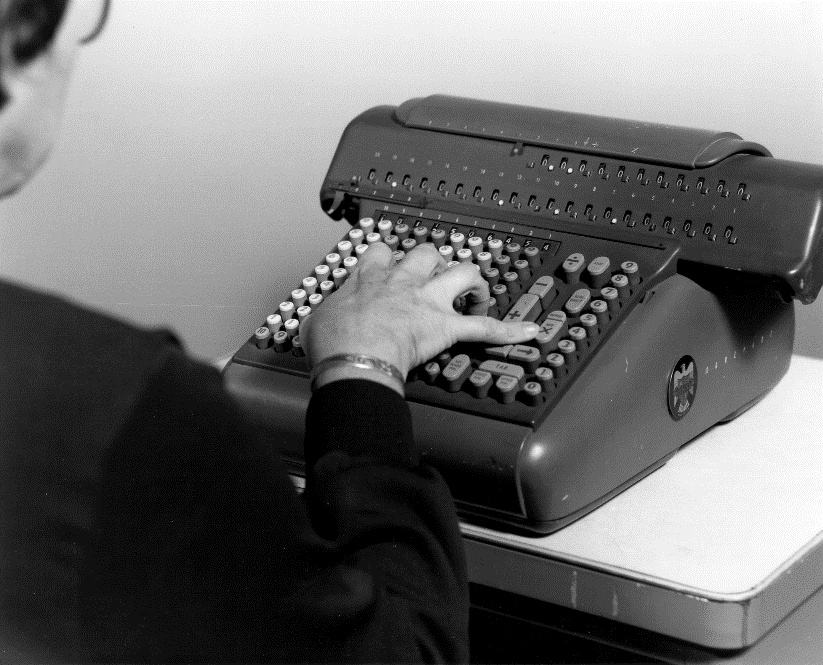
\includegraphics[width=0.55\textwidth]{figures/chapter02/fig2_1_los_alamos_computers.jpg}
    \caption{曼哈顿计划洛斯阿拉莫斯实验室的人工计算团队。在电子计算机普及前，科研人员依靠机械计算器与逐行消元法，求解反应堆临界计算中的大型线性方程组。}
    \label{fig:two-los-alamos-computers}
\end{figure}
\FloatBarrier

在电子计算机尚未普及的年代，求解这样规模的方程组绝非易事。洛斯阿拉莫斯实验室组建了专门的计算小组，动用数十名科研人员与机械台式计算器，以人工流水线的方式逐行迭代计算，完成一次完整的求解需要耗费数周时间。

到了 1945 年，世界第一台电子计算机 ENIAC 建成后，最早的核心任务之一就是为氢弹研制计算中子输运与爆轰流体力学方程组。线性方程组的求解需求，直接推动了早期计算机技术的发展；而计算能力的每一次提升，又反过来让更大规模的线性模型成为可能。

\begin{figure}[htbp]
    \centering
    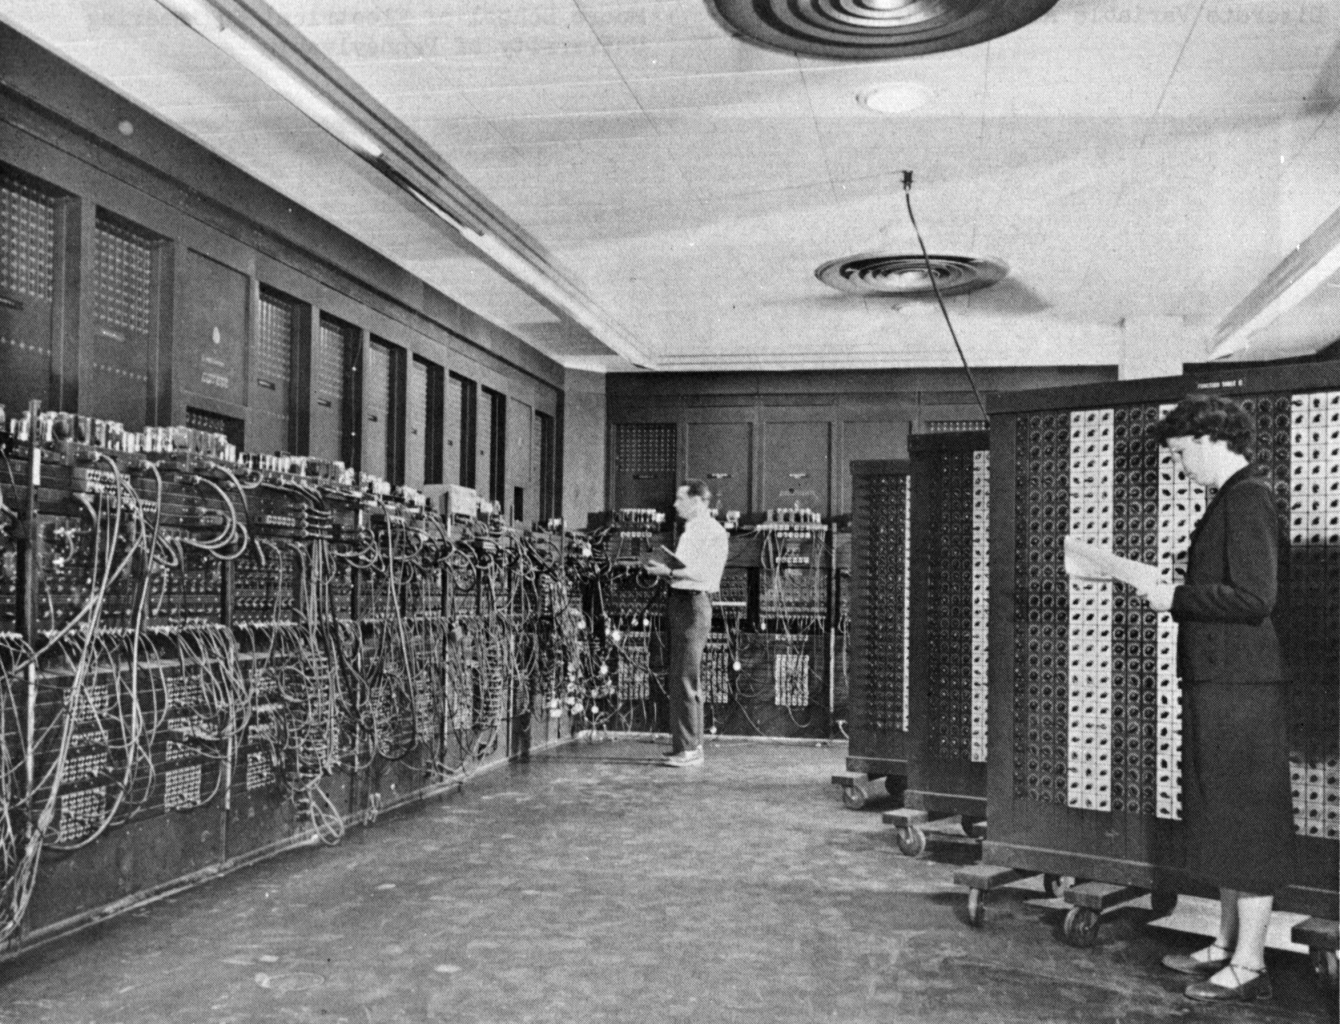
\includegraphics[width=0.55\textwidth]{figures/chapter02/fig2_2_eniac.jpg}
    \caption{世界第一台通用电子计算机ENIAC。大型线性方程组的求解需求，是早期电子计算机最核心的发展动力之一。}
    \label{fig:two-eniac}
\end{figure}
\FloatBarrier

线性代数在应用中的重要性随着计算能力的增强而迅速增加，而每一代新的硬件和软件都引发了对计算能力的更大需求。因此，计算机科学就通过并行处理和大规模计算的爆炸性增长与线性代数密切联系在一起。

科学家和工程师正在研究大量极其复杂的问题，这在几十年前是不可想象的。今天，线性代数对许多科学技术和商业领域中的学生的重要性可以说超过了大学其他数学课程。本书中的材料是在许多有趣领域中作进一步研究的基础。这里举出几个例子，以后将列举其他一些领域。

\begin{itemize}
    \setlength{\itemsep}{5pt}
    \setlength{\parsep}{0pt}
    \item \textbf{核工程与反应堆设计}：从第一代实验堆到现代商用核电站，堆芯物理的数值模拟核心始终是大型稀疏线性方程组的求解，问题规模可达数万甚至数十万阶。
    \item \textbf{石油勘探}：当勘探船寻找海底石油储藏时，它的计算机每天要解几千个线性方程组。方程组的地震数据从气枪的爆炸引起水下冲击波获得。这些冲击波引起海底岩石的震动，并通过用几英里长的电缆拖在船后的地震测波器采集数据。
    \item \textbf{电路设计}：工程师使用仿真软件来设计电路和微芯片，它们包含数百万个晶体管。这样的软件技术依赖于线性代数方法与线性方程组。
    \item \textbf{计算机图形学}：3D 模型的渲染、视角变换、光影计算，本质上都是对顶点向量做线性变换，最终都可归结为线性方程组与矩阵运算。
\end{itemize}

但你或许不知道，这类能决定反应堆临界性、驱动早期计算机发展的大型方程组，其核心解法的思想，我们小学就已经接触过 —— 那就是「鸡兔同笼」问题里的消元思路。从最简单的二元问题，到成百上千未知数的工程模型，底层的逻辑完全一致。

本章我们就从最朴素的鸡兔同笼问题出发，提炼线性方程组的系统求解方法，再引入矩阵这一高效的代数工具，最终把所有线性问题统一为标准形式 $A\boldsymbol{x}=\boldsymbol{b}$。

% 第2章正文；章首原文与两张历史照片保留。
\clearpage
\tcbset{commonbox/.append style={breakable=false,
    fontupper=\linespread{1}\fontsize{11.5pt}{18pt}\selectfont,
    before skip=14pt,after skip=12pt}}
\definecolor{TwoBlue}{HTML}{397AA1}
\definecolor{TwoRose}{HTML}{AC4963}
\definecolor{TwoGreen}{HTML}{448678}
\definecolor{TwoGray}{HTML}{6A747B}
\tikzset{
    twoaxis/.style={-{Stealth[length=2mm]},thin,TwoGray},
    twoblue/.style={-{Stealth[length=2.5mm]},line width=1.1pt,TwoBlue},
    tworose/.style={-{Stealth[length=2.5mm]},line width=1.1pt,TwoRose},
    twoguide/.style={densely dashed,TwoGray!65,thin}
}
\newcommand{\chaptertwofigure}[3]{%
    \par\addvspace{8pt}\noindent\begin{minipage}{\linewidth}
        \centering #3\par\captionof{figure}{#1}\label{#2}
    \end{minipage}\par\addvspace{8pt}}
\newcommand{\twa}{\boldsymbol{a}}
\newcommand{\twb}{\boldsymbol{b}}
\newcommand{\twx}{\boldsymbol{x}}
\newcommand{\twzero}{\boldsymbol{0}}
\newcommand{\twspan}{\operatorname{Span}}
\newcommand{\twaug}[1]{\left(\begin{array}{rrr|r}#1\end{array}\right)}
\newcommand{\twmat}[1]{\left(\begin{array}{rrr}#1\end{array}\right)}
\newcommand{\twcol}[1]{\left(\begin{array}{r}#1\end{array}\right)}

\section{从鸡兔同笼看消元思想}
\label{sec:two-chicken-rabbit}

\subsection*{把数量关系写成方程}

一个笼子里有鸡和兔，共有35个头、94只脚，求鸡和兔各有多少只。设鸡有 $x_1$ 只、兔有 $x_2$ 只，则每只动物对应一个头，鸡有两只脚，兔有四只脚，因而
\begin{equation}
\label{eq:two-chicken-rabbit}
    \begin{cases}
        x_1+x_2=35,\\
        2x_1+4x_2=94.
    \end{cases}
\end{equation}
一组数要成为这个方程组的解，必须\textbf{同时满足两个方程}。例如 $(35,0)$ 满足头数关系，却不满足脚数关系，所以不是方程组的解。

\chaptertwofigure{二元线性方程组的几何意义。两条直线的交点坐标就是方程组的解。}{fig:two-chicken-lines}{%
\begin{tikzpicture}
\begin{axis}[width=.70\textwidth,height=6.1cm,
    axis lines=middle,xmin=0,xmax=50,ymin=0,ymax=39,
    xlabel={$x_1$（鸡）},ylabel={$x_2$（兔）},
    xtick={0,10,23,35,47},ytick={0,12,23.5,35},
    tick label style={font=\footnotesize},clip=false,
    legend style={at={(.5,-.15)},anchor=north,draw=none,font=\small},legend columns=2]
    \addplot[TwoBlue,thick,domain=0:35] {35-x};
    \addlegendentry{$x_1+x_2=35$}
    \addplot[TwoRose,thick,domain=0:47] {23.5-.5*x};
    \addlegendentry{$2x_1+4x_2=94$}
    \draw[twoguide] (axis cs:23,0)--(axis cs:23,12)--(axis cs:0,12);
    \fill[TwoGreen] (axis cs:23,12) circle (2pt)
        node[above right,font=\small,text=TwoGreen] {$(23,12)$};
\end{axis}
\end{tikzpicture}}

图中横坐标表示鸡的数量，纵坐标表示兔的数量。作为实数方程，每个方程对应一条直线；共同的解对应两条直线的交点。原应用还要求 $x_1,x_2$ 为非负整数，求出代数解后，要再检查它是否符合这一要求。

\subsection*{两种消元方法，同一个目的}

\begin{example}[代入消元法]
用\term{substitution}：由第一个方程得 $x_1=35-x_2$，代入第二个方程：
\[
    2(35-x_2)+4x_2=94
    \quad\Longrightarrow\quad 2x_2=24
    \quad\Longrightarrow\quad x_2=12.
\]
再代回 $x_1=35-x_2$，得到 $x_1=23$。因此鸡有23只，兔有12只。
\end{example}

代入之后，第二个方程只含 $x_2$。这正是消元的作用：先把两个未知量之间的关系转化为一个未知量的方程，再恢复另一个未知量。

\begin{example}[加减消元法]
用\term{addition-elimination}，并以 $E_1,E_2$ 分别表示当前的第一、第二个方程。作
\[
    E_2\leftarrow E_2-2E_1,
\]
即用第二个方程减去第一个方程的两倍，\textbf{同时保留第一个方程}，得到
\[
    \begin{cases}x_1+x_2=35,\\2x_2=24.\end{cases}
    \quad\Longrightarrow\quad
    \begin{cases}x_1+x_2=35,\\x_2=12.\end{cases}
\]
后一箭头对应 $E_2\leftarrow\tfrac12 E_2$。这种从下往上求解的过程称为\term{back-substitution}，仍得 $x_2=12$、$x_1=23$。
\end{example}

把所有动物暂时看成鸡，脚数应为 $2\times35=70$；多出的 $94-70=24$ 只脚，每只兔贡献两只，于是兔有12只。这个小学算术过程，对应的恰好就是 $E_2-2E_1$。写成方程后，操作可以推广到更多未知量。

验算得 $23+12=35$、$2\times23+4\times12=94$，且两个数均为非负整数。\textbf{消元的核心是把方程组变成更易求解的形式，同时保持解集不变。}

\subsection*{线性方程与线性方程组}

\begin{definition}[线性方程、解与同解方程组]
关于未知数 $x_1,\ldots,x_n$ 的方程
\[
    a_1x_1+a_2x_2+\cdots+a_nx_n=b
\]
称为\textbf{\term{linear-equation}}，其中 $a_1,\ldots,a_n,b$ 是已知实数，右端 $b$ 称为\term{constant-term}。由若干这样的方程组成的整体称为\textbf{\term{linear-system}}。

同时满足其中每个方程的一组有序数，称为方程组的一个\textbf{\term{solution}}；全体解构成\textbf{\term{solution-set}}。解集相同的两个方程组称为\textbf{\term{equivalent-systems}}。
\end{definition}

线性方程中未知数只以一次项出现，彼此不相乘。例如 $2x_1-3x_2=1$ 是线性方程，而 $x_1x_2=1$、$x_1^2+x_2=1$ 都不是。系数可以为0；消元中出现的 $0=0$ 或 $0=1$ 也必须纳入讨论。

由 $m$ 个方程组成的 $n$ 元线性方程组的一般形式是
\begin{equation}
\label{eq:two-general-system}
\begin{cases}
 a_{11}x_1+a_{12}x_2+\cdots+a_{1n}x_n=b_1,\\
 a_{21}x_1+a_{22}x_2+\cdots+a_{2n}x_n=b_2,\\
 \hspace{35mm}\vdots\\
 a_{m1}x_1+a_{m2}x_2+\cdots+a_{mn}x_n=b_m.
\end{cases}
\end{equation}
这里 $m$ 是方程个数，$n$ 是未知数个数，两者不必相等。解通常写为列向量 $\twx=(x_1,\ldots,x_n)^{\mathrm T}$。

\subsection*{三种同解初等变换}

\begin{theorem}[线性方程组的初等变换]
下列三种操作都保持方程组的解集不变：

\textbf{交换：}交换两个方程的位置，记为 $E_i\leftrightarrow E_j$。

\textbf{倍乘：}用非零实数 $c$ 乘一个方程的两边，记为 $E_i\leftarrow cE_i$，其中 $c\ne0$。

\textbf{倍加：}把一个方程的 $c$ 倍加到另一个方程上，记为 $E_i\leftarrow E_i+cE_j$，其中 $i\ne j$；方程 $E_j$ 保持不变。

它们称为方程组的\textbf{\term{elementary-equation}}。
\end{theorem}

\begin{proof}
交换只改变书写次序。倍乘后，可以再乘 $1/c$ 恢复原方程。倍加后，保留着 $E_j$，再作 $E_i\leftarrow E_i-cE_j$ 就能恢复原方程。因此每一步的解既满足变换前的方程组，也满足变换后的方程组，反过来同样成立。
\end{proof}

\begin{corollary}[连续变换仍然同解]
有限次初等变换得到的方程组与原方程组同解。消元时只要每一步都合法，最后求出的就是原方程组的全部解。
\end{corollary}

注意倍乘的数不能为0，否则原方程的信息会丢失。例如 $x_1=1$ 乘0后变成 $0=0$，任意 $x_1$ 都满足后者。倍加时也不能只留下相加得到的一个方程、同时删去原来的两个方程。

从图\ref{fig:two-chicken-lines}看，消元后两个单独的方程所表示的直线可以改变，但共同交点不变。我们希望逐步得到这样的形式：上面的方程可以含较多未知数，下面的方程依次消去前面的未知数。这就是下一节要建立的\textbf{\term{echelon-system}}；再从下往上回代，完成求解。

\section{高斯消元法：从二元到 $n$ 元}
\label{sec:two-gauss}

\subsection*{贯穿本章的三元例题}

\begin{example}[由三个方程逐步消元]
求解
\begin{equation}
\label{eq:two-main-system}
    \begin{cases}
        x_1+x_2+x_3=6,\\
        2x_1-x_2+x_3=3,\\
        x_1+2x_2-x_3=2.
    \end{cases}
\end{equation}
\end{example}

\textbf{第一步：用第一个方程消去下面两个方程中的 $x_1$。}依次作
\[
 E_2\leftarrow E_2-2E_1,\qquad E_3\leftarrow E_3-E_1.
\]
逐项计算有
\[
\begin{aligned}
 (2x_1-x_2+x_3)-2(x_1+x_2+x_3)&=3-2\times6,\\
 (x_1+2x_2-x_3)-(x_1+x_2+x_3)&=2-6.
\end{aligned}
\]
因此原方程组化为
\[
    \begin{cases}
        x_1+x_2+x_3=6,\\
        -3x_2-x_3=-9,\\
        x_2-2x_3=-4.
    \end{cases}
\]

\textbf{第二步：选择方便的方程继续消去 $x_2$。}第三个方程的 $x_2$ 系数为1，先作 $E_2\leftrightarrow E_3$，再作 $E_3\leftarrow E_3+3E_2$：
\begin{equation}
\label{eq:two-main-echelon}
    \begin{cases}
        x_1+x_2+x_3=6,\\
        x_2-2x_3=-4,\\
        -7x_3=-21.
    \end{cases}
\end{equation}
此处最后一式来自 $(-3x_2-x_3)+3(x_2-2x_3)=-9+3(-4)$。每一个新方程都按同样的规则处理了左右两边。

\textbf{第三步：从最后一个方程开始回代。}
\[
    -7x_3=-21\Rightarrow x_3=3,
    \qquad x_2=-4+2x_3=2,
    \qquad x_1=6-x_2-x_3=1.
\]
所以唯一解为 $\twx=(1,2,3)^{\mathrm T}$。代入原式，左边依次为 $6,3,2$，与右边相同。变量从两个增加到三个，但方法没有改变：\textbf{先通过同解变换减少未知数，再利用已经求出的量回代。}

\chaptertwofigure{三元线性方程组的几何意义。三个平面两两相交，三条交线共同经过点 $P(1,2,3)$，它的坐标就是方程组的唯一解。浅色区域仅表示各平面的一部分，粗线突出两两交线。}{fig:two-three-planes}{%
\begin{tikzpicture}[x={(.8cm,.5427cm)},y={(-.6cm,.7236cm)},z={(0cm,.4264cm)},font=\small,
    pairline/.style={line width=1.25pt},
    linelabel/.style={fill=white,inner sep=1.5pt,font=\footnotesize}]
    % Orthographic view with unequal projected axis slopes to retain depth; coordinates are actual (x1,x2,x3).
    \coordinate (P) at (1,2,3);
    % Coordinate axes and the projection of P onto the horizontal coordinate plane.
    \draw[twoaxis] (0,0,0)--(5.2,0,0) node[right] {$x_1$};
    \draw[twoaxis] (0,0,0)--(0,6.5,0) node[left] {$x_2$};
    \draw[twoaxis] (0,0,0)--(0,0,12) node[above] {$x_3$};
    \node[below] at (0,0,0) {$O$};
    \draw[twoguide] (1,0,0)--(1,2,0)--(0,2,0);
    \draw[twoguide] (1,2,0)--(P);
    \node[below right,font=\footnotesize] at (1,0,0) {$1$};
    \node[below left,font=\footnotesize] at (0,2,0) {$2$};
    % Plane patches use in-plane directions; grids emphasize distinct spatial tilts.
    \filldraw[fill=TwoBlue,fill opacity=.14,draw=TwoBlue!85,line width=.6pt] (-2.2000,2.8000,5.4000)--(1.8000,-1.2000,5.4000)--(4.2000,1.2000,0.6000)--(0.2000,5.2000,0.6000)--cycle;
    \draw[TwoBlue!35,very thin] (-1.4000,2.0000,5.4000)--(1.0000,4.4000,0.6000);
    \draw[TwoBlue!35,very thin] (-1.7200,3.2800,4.4400)--(2.2800,-0.7200,4.4400);
    \draw[TwoBlue!35,very thin] (-0.6000,1.2000,5.4000)--(1.8000,3.6000,0.6000);
    \draw[TwoBlue!35,very thin] (-1.2400,3.7600,3.4800)--(2.7600,-0.2400,3.4800);
    \draw[TwoBlue!35,very thin] (0.2000,0.4000,5.4000)--(2.6000,2.8000,0.6000);
    \draw[TwoBlue!35,very thin] (-0.7600,4.2400,2.5200)--(3.2400,0.2400,2.5200);
    \draw[TwoBlue!35,very thin] (1.0000,-0.4000,5.4000)--(3.4000,2.0000,0.6000);
    \draw[TwoBlue!35,very thin] (-0.2800,4.7200,1.5600)--(3.7200,0.7200,1.5600);
    \filldraw[fill=TwoGreen,fill opacity=.14,draw=TwoGreen!85,line width=.6pt] (-0.3000,0.8000,4.4000)--(2.3000,0.8000,-0.8000)--(2.3000,3.2000,1.6000)--(-0.3000,3.2000,6.8000)--cycle;
    \draw[TwoGreen!35,very thin] (0.2200,0.8000,3.3600)--(0.2200,3.2000,5.7600);
    \draw[TwoGreen!35,very thin] (-0.3000,1.2800,4.8800)--(2.3000,1.2800,-0.3200);
    \draw[TwoGreen!35,very thin] (0.7400,0.8000,2.3200)--(0.7400,3.2000,4.7200);
    \draw[TwoGreen!35,very thin] (-0.3000,1.7600,5.3600)--(2.3000,1.7600,0.1600);
    \draw[TwoGreen!35,very thin] (1.2600,0.8000,1.2800)--(1.2600,3.2000,3.6800);
    \draw[TwoGreen!35,very thin] (-0.3000,2.2400,5.8400)--(2.3000,2.2400,0.6400);
    \draw[TwoGreen!35,very thin] (1.7800,0.8000,0.2400)--(1.7800,3.2000,2.6400);
    \draw[TwoGreen!35,very thin] (-0.3000,2.7200,6.3200)--(2.3000,2.7200,1.1200);
    \filldraw[fill=TwoRose,fill opacity=.14,draw=TwoRose!85,line width=.6pt] (-1.2500,2.0000,0.7500)--(2.3500,0.2000,0.7500)--(3.2500,2.0000,5.2500)--(-0.3500,3.8000,5.2500)--cycle;
    \draw[TwoRose!35,very thin] (-0.5300,1.6400,0.7500)--(0.3700,3.4400,5.2500);
    \draw[TwoRose!35,very thin] (-1.0700,2.3600,1.6500)--(2.5300,0.5600,1.6500);
    \draw[TwoRose!35,very thin] (0.1900,1.2800,0.7500)--(1.0900,3.0800,5.2500);
    \draw[TwoRose!35,very thin] (-0.8900,2.7200,2.5500)--(2.7100,0.9200,2.5500);
    \draw[TwoRose!35,very thin] (0.9100,0.9200,0.7500)--(1.8100,2.7200,5.2500);
    \draw[TwoRose!35,very thin] (-0.7100,3.0800,3.4500)--(2.8900,1.2800,3.4500);
    \draw[TwoRose!35,very thin] (1.6300,0.5600,0.7500)--(2.5300,2.3600,5.2500);
    \draw[TwoRose!35,very thin] (-0.5300,3.4400,4.3500)--(3.0700,1.6400,4.3500);
    \draw[pairline,TwoBlue!60!TwoGreen] (-0.3000,1.3500,4.9500)--(2.3000,2.6500,1.0500) node[linelabel,below right] {$\ell_{12}$};
    \draw[pairline,TwoBlue!55!TwoRose] (2.6875,0.8750,2.4375)--(-0.6875,3.1250,3.5625) node[linelabel,left] {$\ell_{13}$};
    \draw[pairline,TwoGreen!55!TwoRose] (1.4000,0.8000,1.0000)--(0.6000,3.2000,5.0000) node[linelabel,above left] {$\ell_{23}$};
    \fill[white] (P) circle (3.5pt);
    \fill[black] (P) circle (2.3pt);
    \draw[black!75,thin] (P)--(2.8cm,1.4cm)
        node[anchor=west,fill=white,inner sep=2pt] {$P(1,2,3)$};
    \node[anchor=west,text=TwoBlue] at (4.7cm,5.6cm) {$\Pi_1:\ x_1+x_2+x_3=6$};
    \node[anchor=west,text=TwoGreen] at (4.7cm,5.05cm) {$\Pi_2:\ 2x_1-x_2+x_3=3$};
    \node[anchor=west,text=TwoRose] at (4.7cm,4.5cm) {$\Pi_3:\ x_1+2x_2-x_3=2$};
    \node[anchor=west,align=left,font=\footnotesize] at (4.7cm,3.4cm)
        {$\ell_{12}=\Pi_1\cap\Pi_2$\\[4pt]
         $\ell_{13}=\Pi_1\cap\Pi_3$\\[4pt]
         $\ell_{23}=\Pi_2\cap\Pi_3$};
\end{tikzpicture}}

三个平面两两相交，并不自动保证三个平面有同一个交点。本例有且只有一个公共点，是由消元结果确定的，不能仅凭透视图判断。

\subsection*{主元、行阶梯形与自由变量}

\begin{definition}[方程组的行阶梯形]
固定未知数次序 $x_1,\ldots,x_n$，把方程右端的常数项也看成书写在系数之后的一项。

对左端不全为0的方程，\textbf{第一个非零系数}称为该行的\textbf{\term{pivot}}，它所在的未知数称为\textbf{\term{basic-variable}}。

若所有 $0=0$ 的全零方程位于最下方，且其余各行从上到下第一个非零项的位置严格右移，就称方程组为\textbf{行阶梯形方程组}。若出现 $0=c$（$c\ne0$），将其非零常数看作位于所有未知数之后；它表示矛盾，而不对应主元变量。

在没有矛盾方程的行阶梯形中，不属于主元变量的未知数称为\textbf{\term{free-variable}}。
\end{definition}

主元是一个\textbf{非零数}，主元变量是它对应的\textbf{未知数}，两者需要区分。例如式\eqref{eq:two-main-echelon}的主元依次为 $1,1,-7$，主元变量依次为 $x_1,x_2,x_3$。主元不必等于1。

“逐行右移”说的是\textbf{首个非零位置}，不要求每往下一行恰好少一个非零项，也不要求它恰好移到紧邻的一列。例如
\[
    \begin{cases}
        x_1+2x_2-x_3+x_4=3,\\
        \hspace{24mm}x_3+x_4=2
    \end{cases}
\]
已经是行阶梯形。主元变量为 $x_1,x_3$，$x_2,x_4$ 是自由变量。令 $x_2=s$、$x_4=t$，则
\[
    x_3=2-t,\qquad x_1=5-2s-2t,\qquad s,t\in\mathbb R.
\]
“自由”指可以独立指定这两个参数；一旦指定，主元变量就随之确定。\textbf{只有在方程组有解时，才可以把自由变量任意取值并得到解。}这里\term{consistent}也称相容，\term{inconsistent}也称不相容。

上述方法推广到一般方程组，就是\term{gaussian}。

\begin{theorem}[高斯消元法的基本步骤]
\textbf{\term{forward-elimination}：}从最左侧尚未处理的未知数开始，在尚未使用的方程中寻找该未知数的非零系数；需要时交换方程，再用倍加消去它下方的系数。

\textbf{逐步推进：}移到下一行、右侧各列，重复上述过程；若某列在剩余各行中全为0，就跳过该列。最终得到行阶梯形。

\textbf{判断并回代：}先检查有无矛盾方程。若没有，指定自由变量，再从最后一个非零方程开始回代，求出所有主元变量。
\end{theorem}

每次只能用已经选定的非零系数作为消元依据。若当前系数为0，可以向下寻找并交换；若这一列下方全为0，就改看右边一列，不能把0当作除数。未知数的次序在本章始终固定。

\subsection*{消元结果怎样告诉我们解的个数}

\begin{example}[无解：出现矛盾]
对方程组
\[
    \begin{cases}x_1+x_2=2,\\2x_1+2x_2=5,\end{cases}
    \qquad E_2\leftarrow E_2-2E_1,
\]
得到 $x_1+x_2=2$、$0=1$。不存在任何一组数能满足 $0=1$，所以原方程组\textbf{无解}。
\end{example}

\begin{example}[唯一解：每个未知数都有主元]
对方程组
\[
    \begin{cases}x_1+x_2=2,\\x_1-x_2=0,\end{cases}
    \quad\xrightarrow{E_2\leftarrow E_2-E_1}\quad
    \begin{cases}x_1+x_2=2,\\-2x_2=-2,\end{cases}
\]
回代得到 $x_2=1$、$x_1=1$。没有矛盾，也没有自由变量，所以有\textbf{\term{unique}}。
\end{example}

\begin{example}[无穷多解：有自由变量]
对方程组
\[
    \begin{cases}x_1+x_2=2,\\2x_1+2x_2=4,\end{cases}
    \quad\xrightarrow{E_2\leftarrow E_2-2E_1}\quad
    \begin{cases}x_1+x_2=2,\\0=0,\end{cases}
\]
第二式不再增加限制。令 $x_2=t$，就有 $x_1=2-t$，因此全部解为
\[
    \twx=(2-t,t)^{\mathrm T},\qquad t\in\mathbb R.
\]
不同的 $t$ 给出不同的解，所以方程组有\textbf{\term{infinite-solutions}}。
\end{example}

\chaptertwofigure{二元线性方程组解的三种情形。每个子图中的曲线对应上面相应例题的方程；重合的两条直线用粗实线与虚线区分。}{fig:two-three-cases}{%
\begin{tikzpicture}[font=\small]
\begin{scope}[shift={(0,0)}]
    \draw[twoaxis] (-.3,0)--(2.8,0) node[right] {$x_1$};
    \draw[twoaxis] (0,-.3)--(0,2.9) node[above] {$x_2$};
    \draw[TwoBlue,thick] (-.2,2.2)--(2.2,-.2);
    \draw[TwoRose,thick] (-.2,-.2)--(2.35,2.35);
    \fill[black] (1,1) circle (1.8pt) node[above right] {$(1,1)$};
    \node at (1.2,-.9) {(a) 唯一解};
\end{scope}
\begin{scope}[shift={(4.8,0)}]
    \draw[twoaxis] (-.3,0)--(2.8,0) node[right] {$x_1$};
    \draw[twoaxis] (0,-.3)--(0,2.9) node[above] {$x_2$};
    \draw[TwoBlue,thick] (-.2,2.2)--(2.2,-.2);
    \draw[TwoRose,thick] (-.2,2.7)--(2.7,-.2);
    \node at (1.2,-.9) {(b) 无解};
\end{scope}
\begin{scope}[shift={(9.6,0)}]
    \draw[twoaxis] (-.3,0)--(2.8,0) node[right] {$x_1$};
    \draw[twoaxis] (0,-.3)--(0,2.9) node[above] {$x_2$};
    \draw[TwoBlue,line width=2pt] (-.2,2.2)--(2.2,-.2);
    \draw[TwoRose,dashed,line width=1pt] (-.2,2.2)--(2.2,-.2);
    \fill[TwoGreen] (.7,1.3) circle (1.8pt) node[above right] {$(2-t,t)$};
    \node at (1.2,-.9) {(c) 无穷多解};
\end{scope}
\end{tikzpicture}}

\begin{theorem}[由行阶梯形判断解的个数]
对 $n$ 元实线性方程组，先用初等变换得到行阶梯形。

若出现 $0=c$（$c\ne0$），则\textbf{无解}。

在\textbf{没有矛盾方程}的前提下，设主元变量有 $p$ 个：若 $p=n$，则有唯一解；若 $p<n$，则有 $n-p$ 个自由变量，从而有无穷多解。
\end{theorem}

\begin{corollary}[实线性方程组解的三分性]
实线性方程组只有无解、唯一解、无穷多解三种可能，不会恰好有两个或三个不同的解。\textbf{一旦方程组有解且存在自由变量，就可以让参数在实数范围内连续取值。}
\end{corollary}

零方程 $0=0$ 与矛盾方程 $0=c$ 必须分清。出现零方程并不一定有无穷多解，例如 $x_1=1$、$x_2=2$、$0=0$ 仍然唯一确定两个未知数。反过来，方程数等于未知数个数，也不保证存在唯一解。

\subsection*{在三维中看自由变量}

例如 $x_1=1$、$x_2=2$ 两个方程留下自由变量 $x_3=t$，解为 $(1,2,t)^{\mathrm T}$，在空间中是一条直线。如果只有 $x_3=0$ 这一个有效方程，便有两个自由变量，解为 $(s,t,0)^{\mathrm T}$，构成一个平面。这些图形是\textbf{解向量所在的集合}。

\chaptertwofigure{自由变量与解集的形状。左图两个平面交成一条直线，用一个参数表示解；右图解集本身是一个平面，需要两个参数。}{fig:two-free-geometry}{%
\begin{tikzpicture}[font=\small,x={(.9cm,-.22cm)},y={(.55cm,.32cm)},z={(0cm,.8cm)}]
\begin{scope}
    \draw[twoaxis] (0,0,0)--(3.4,0,0) node[right] {$x_1$};
    \draw[twoaxis] (0,0,0)--(0,3.6,0) node[above] {$x_2$};
    \draw[twoaxis] (0,0,0)--(0,0,3.3) node[above] {$x_3$};
    \filldraw[fill=TwoBlue,fill opacity=.16,draw=TwoBlue]
        (1,0,-.4)--(1,3,-.4)--(1,3,3)--(1,0,3)--cycle;
    \filldraw[fill=TwoGreen,fill opacity=.17,draw=TwoGreen]
        (-.2,2,-.4)--(2.5,2,-.4)--(2.5,2,3)--(-.2,2,3)--cycle;
    \draw[TwoRose,line width=1.4pt] (1,2,-.5)--(1,2,3.35)
        node[above] {$(1,2,t)$};
    \node[below] at (1.1,1,-1.1) {一个自由变量：直线};
\end{scope}
\begin{scope}[shift={(7.5cm,0cm)}]
    \filldraw[fill=TwoBlue,fill opacity=.13,draw=TwoBlue]
        (-.5,-.5,0)--(3,-.5,0)--(3,3,0)--(-.5,3,0)--cycle;
    \draw[twoaxis] (0,0,0)--(3.4,0,0) node[right] {$x_1$};
    \draw[twoaxis] (0,0,0)--(0,3.6,0) node[above] {$x_2$};
    \draw[twoaxis] (0,0,0)--(0,0,3.3) node[above] {$x_3$};
    \fill[TwoRose] (1.4,1.6,0) circle (1.9pt) node[above right] {$(s,t,0)$};
    \node[below] at (1.1,1,-1.1) {两个自由变量：平面};
\end{scope}
\end{tikzpicture}}

高维解集不一定能画出来，但自由变量的含义不变：它们记录全部解所需要的独立参数。不能把“有几个方程”直接当成“有几个独立限制”，是否重复要通过消元辨认。

\section{矩阵与初等行变换}
\label{sec:two-matrices}

\subsection*{把反复出现的未知数暂时省去}

在前面的计算中，$x_1,x_2,x_3$ 的位置始终固定，真正发生变化的是它们的系数与方程右端的常数。只要约定列的次序，就可以把这些数排成一个数表，省去重复书写的未知数和等号。

\begin{definition}[矩阵、系数矩阵与增广矩阵]
由 $m\times n$ 个数按照 $m$ 行、$n$ 列排列成的矩形数表，称为一个\textbf{$m\times n$ 矩阵}，记作 $A=(a_{ij})_{m\times n}$。其中 $a_{ij}$ 是第 $i$ 行、第 $j$ 列的元素。

对于式\eqref{eq:two-general-system}，按未知数次序排成的
\[
 A=\left(\begin{array}{cccc}
 a_{11}&a_{12}&\cdots&a_{1n}\\
 a_{21}&a_{22}&\cdots&a_{2n}\\
 \vdots&\vdots&&\vdots\\
 a_{m1}&a_{m2}&\cdots&a_{mn}
 \end{array}\right)
\]
称为\textbf{\term{coefficient-matrix}}。把常数项列 $\twb=(b_1,\ldots,b_m)^{\mathrm T}$ 附在右边，得到\textbf{\term{augmented}}
\[
 \overline A=(A\mid\twb)
 =\left(\begin{array}{cccc|c}
 a_{11}&a_{12}&\cdots&a_{1n}&b_1\\
 a_{21}&a_{22}&\cdots&a_{2n}&b_2\\
 \vdots&\vdots&&\vdots&\vdots\\
 a_{m1}&a_{m2}&\cdots&a_{mn}&b_m
 \end{array}\right).
\]
系数矩阵有 $n$ 列，增广矩阵有 $n+1$ 列；竖线只用来区分系数列与常数项列。
\end{definition}

一个方程对应一行，一个未知数对应一个系数列。某个未知数没有出现时，其系数必须填0，不能跳过这一列。增广矩阵右端的常数项列并不代表一个新增的未知数。

鸡兔同笼方程组的两种矩阵分别为
\[
 A=\left(\begin{array}{rr}1&1\\2&4\end{array}\right),
 \qquad
 \overline A=\left(\begin{array}{rr|r}1&1&35\\2&4&94\end{array}\right).
\]
贯穿例题\eqref{eq:two-main-system}的两种矩阵则为
\[
 A=\twmat{1&1&1\\2&-1&1\\1&2&-1},
 \qquad
 \overline A=\twaug{1&1&1&6\\2&-1&1&3\\1&2&-1&2}.
\]
从增广矩阵的第2行读回去，就是 $2x_1-x_2+x_3=3$。能够在方程和数表之间双向转换，才真正理解了这种记法。

\subsection*{方程操作与行操作一一对应}

\begin{definition}[矩阵的初等行变换]
用 $R_i$ 表示当前矩阵的第 $i$ 行。下列操作称为\textbf{\term{elementary-row}}：
\[
\begin{array}{ll}
 R_i\leftrightarrow R_j & \text{交换两行；}\\[3pt]
 R_i\leftarrow cR_i\quad(c\ne0) & \text{用非零数乘一行；}\\[3pt]
 R_i\leftarrow R_i+cR_j\quad(i\ne j) & \text{把一行的倍数加到另一行。}
\end{array}
\]
可经过有限次初等行变换互相得到的两个矩阵称为\textbf{\term{row-equivalent}}，本章用 $\sim$ 或标有操作的箭头表示。
\end{definition}

\begin{theorem}[增广矩阵行变换保持解集]
对增广矩阵作初等行变换，等价于对方程组作相应的同解初等变换。因而行变换前后的增广矩阵表示同解方程组。
\end{theorem}

理由是每一行的系数与常数项共同记录一个方程，两边始终按同一操作改变。\textbf{常数项列必须与系数列一起变换。}只改变系数而不改变常数项，一般就改变了原来的问题。

例如鸡兔同笼的加减消元可压缩为
\[
 \left(\begin{array}{rr|r}1&1&35\\2&4&94\end{array}\right)
 \xrightarrow{R_2\leftarrow R_2-2R_1}
 \left(\begin{array}{rr|r}1&1&35\\0&2&24\end{array}\right)
 \xrightarrow{R_2\leftarrow\frac12 R_2}
 \left(\begin{array}{rr|r}1&1&35\\0&1&12\end{array}\right).
\]
从末行读出 $x_2=12$，回代第一行得 $x_1=23$。数表的写法省去了符号，却保留了完整的计算信息。

\subsection*{同一个三元例题：方程与矩阵对照}

以下每一行左侧是方程组，右侧是同一步骤的增广矩阵。所有行号均指\textbf{当前}的行，而不是原始方程中永远固定的编号。

\textbf{起点：}
\[
 \begin{array}{c@{\qquad\longleftrightarrow\qquad}c}
 \begin{cases}x_1+x_2+x_3=6,\\2x_1-x_2+x_3=3,\\x_1+2x_2-x_3=2\end{cases}
 &\twaug{1&1&1&6\\2&-1&1&3\\1&2&-1&2}
 \end{array}
\]

\textbf{第一次倍加：}$E_2\leftarrow E_2-2E_1$ 对应 $R_2\leftarrow R_2-2R_1$。
\[
 \begin{array}{c@{\qquad\longleftrightarrow\qquad}c}
 \begin{cases}x_1+x_2+x_3=6,\\-3x_2-x_3=-9,\\x_1+2x_2-x_3=2\end{cases}
 &\twaug{1&1&1&6\\0&-3&-1&-9\\1&2&-1&2}
 \end{array}
\]

\textbf{第二次倍加：}$E_3\leftarrow E_3-E_1$ 对应 $R_3\leftarrow R_3-R_1$。
\[
 \begin{array}{c@{\qquad\longleftrightarrow\qquad}c}
 \begin{cases}x_1+x_2+x_3=6,\\-3x_2-x_3=-9,\\x_2-2x_3=-4\end{cases}
 &\twaug{1&1&1&6\\0&-3&-1&-9\\0&1&-2&-4}
 \end{array}
\]

\textbf{交换：}$E_2\leftrightarrow E_3$ 对应 $R_2\leftrightarrow R_3$。
\[
 \begin{array}{c@{\qquad\longleftrightarrow\qquad}c}
 \begin{cases}x_1+x_2+x_3=6,\\x_2-2x_3=-4,\\-3x_2-x_3=-9\end{cases}
 &\twaug{1&1&1&6\\0&1&-2&-4\\0&-3&-1&-9}
 \end{array}
\]

\textbf{继续倍加：}$E_3\leftarrow E_3+3E_2$ 对应 $R_3\leftarrow R_3+3R_2$。
\begin{equation}
\label{eq:two-main-echelon-matrix}
 \begin{array}{c@{\qquad\longleftrightarrow\qquad}c}
 \begin{cases}x_1+x_2+x_3=6,\\x_2-2x_3=-4,\\-7x_3=-21\end{cases}
 &\twaug{1&1&1&6\\0&1&-2&-4\\0&0&-7&-21}
 \end{array}
\end{equation}

每一步的全部数值都来自前一行的方程操作。矩阵行变换没有增加新的求解原理，只是使同一个原理更便于书写与实现。

\subsection*{行阶梯形矩阵}

\begin{definition}[主元位置与行阶梯形矩阵]
矩阵非零行的第一个非零元素称为该行的\textbf{主元}；它所在的位置称为\textbf{\term{pivot-position}}，所在列称为\textbf{\term{pivot-column}}。

满足以下条件的矩阵称为\textbf{\term{row-echelon}}：

\textbf{零行在底：}所有元素都为0的行位于所有非零行的下方。

\textbf{主元右移：}每个非零行的主元位置，都在上一非零行的主元位置右边。

因此，每个主元下方的元素都为0。所有元素均为0的\term{zero-matrix}也视为行阶梯形矩阵。
\end{definition}

% ===== 一般阶梯形结构图开始 =====
\chaptertwofigure{一般阶梯形矩阵的结构示意。$\blacksquare$ 表示主元，$\ast$ 表示任意非零元，$0$ 表示零。主元逐行右移，主元下方为零，零行位于底部。}{fig:two-echelon-structure}{%
\begingroup
\renewcommand{\arraystretch}{1.3}
\setlength{\arraycolsep}{9pt}
\[
    \begin{bmatrix}
        \blacksquare & \ast & \ast & \ast & \ast & \ast \\
        0 & 0 & \blacksquare & \ast & \ast & \ast \\
        0 & 0 & 0 & 0 & \blacksquare & \ast \\
        0 & 0 & 0 & 0 & 0 & 0
    \end{bmatrix}
\]
\endgroup}

图中展示一种可能的非零分布，并不要求主元右侧的元素全部非零；主元之间也可以跳过没有主元的列。
% ===== 一般阶梯形结构图结束 =====

例如
\[
 H=\left(\begin{array}{rrrr|r}
 \textcolor{TwoRose}{2}&-1&3&0&4\\
 0&0&\textcolor{TwoRose}{-5}&2&1\\
 0&0&0&0&0
 \end{array}\right)
\]
是行阶梯形矩阵。主元为 $2,-5$，对应第1、3列，主元之间可以跳过某些列。如果将它看作四元方程组的增广矩阵，则 $x_2,x_4$ 是自由变量。

又如
\[
 \left(\begin{array}{rr|r}1&2&3\\0&0&1\end{array}\right)
\]
也是行阶梯形，但其末行的主元落在\textbf{常数项列}，代表 $0=1$，原方程组无解。讨论解时，必须区分系数部分的主元与增广列中的主元。

\begin{corollary}[行阶梯形的存在]
任意矩阵都可以通过有限次初等行变换化成行阶梯形。其具体数值形式可以因选取的行变换不同而不同。
\end{corollary}

这直接来自高斯消元的过程：每次选定的主元向下、向右推进，行数和列数有限，所以过程最终停止。对增广矩阵消元时，如果常数项列出现主元，就已经足以判断无解。

\section{行最简形与高斯--若尔当消元法}
\label{sec:two-gauss-jordan}

\subsection*{把主元上方也消成0}

行阶梯形消去了主元下方的元素，但其上方通常仍有非零元素，所以要回代。若再把每个主元化为1，并把它上方的元素也消为0，就能够从结果中直接读出主元变量。

\begin{definition}[行最简形矩阵]
一个行阶梯形矩阵，如果还满足：

\textbf{主元为1：}每个非零行的主元均为1；

\textbf{主元列其余元素为0：}每个主元所在列中，除该主元外的所有元素都为0，

就称为\textbf{\term{reduced-echelon}}，也称简化行阶梯形矩阵。
\end{definition}

% ===== 简化阶梯形结构图开始 =====
\chaptertwofigure{简化阶梯形矩阵的结构示意。$\blacksquare$ 表示主元，$\ast$ 表示任意非零元，$0$ 表示零。此图中的主元均取值为1，且主元所在列的其余元素全部为零。}{fig:two-reduced-echelon-structure}{%
\begingroup
\renewcommand{\arraystretch}{1.3}
\setlength{\arraycolsep}{9pt}
\[
    \begin{bmatrix}
        \blacksquare & \ast & 0 & \ast & 0 & \ast \\
        0 & 0 & \blacksquare & \ast & 0 & \ast \\
        0 & 0 & 0 & 0 & \blacksquare & \ast \\
        0 & 0 & 0 & 0 & 0 & 0
    \end{bmatrix}
\]
\endgroup}
% ===== 简化阶梯形结构图结束 =====

例如
\[
 \left(\begin{array}{rrrr|r}
 1&2&0&-1&3\\0&0&1&4&2\\0&0&0&0&0
 \end{array}\right)
\]
已经是行最简形。第2、4列没有主元，其中仍可有非零元素。\textbf{行最简形不要求所有非主元元素都为0，只要求主元所在列满足这一条件。}

\begin{theorem}[行最简形的存在与唯一性]
每个矩阵都可以用初等行变换化为行最简形；虽然化简步骤可以不同，最终的行最简形是唯一的。
\end{theorem}

存在性可由行阶梯形继续消元得到。唯一性是行化简的基本结论，本章先使用这一结论，不展开其一般证明。它使不同计算路径的结果能够相互核对；不能把不同的行阶梯形误认为求解结果必然不同。

\subsection*{用高斯--若尔当法重做三元例题}

在高斯消元得到行阶梯形后，从最后一个主元向上处理：先把主元化为1，再消去同列上方的元素。这一过程称为\textbf{\term{gauss-jordan}}。

\begin{example}[从行阶梯形到直接读解]
将式\eqref{eq:two-main-system}的增广矩阵化为行最简形，求出方程组的解。
\end{example}

\textbf{解：}由式\eqref{eq:two-main-echelon-matrix}继续作行变换：
\[
 \twaug{1&1&1&6\\0&1&-2&-4\\0&0&-7&-21}
 \xrightarrow{R_3\leftarrow-\frac17R_3}
 \twaug{1&1&1&6\\0&1&-2&-4\\0&0&1&3}.
\]
用第三行消去它上方第3列的非零元素：
\[
 \xrightarrow{R_2\leftarrow R_2+2R_3}
 \twaug{1&1&1&6\\0&1&0&2\\0&0&1&3}
 \xrightarrow{R_1\leftarrow R_1-R_3}
 \twaug{1&1&0&3\\0&1&0&2\\0&0&1&3}.
\]
最后用第二行消去第1行中的 $x_2$ 系数：
\[
 \xrightarrow{R_1\leftarrow R_1-R_2}
 \twaug{1&0&0&1\\0&1&0&2\\0&0&1&3}.
\]
现在可以直接读出 $x_1=1$、$x_2=2$、$x_3=3$，不必另作回代。

\subsection*{有自由变量时，直接读出的是参数关系}

\begin{example}[由行最简形写出全部解]
对四元方程组
\[
    \begin{cases}
    x_1+2x_2-x_3+x_4=3,\\
    2x_1+4x_2+x_3+5x_4=12,
    \end{cases}
\]
作 $R_2\leftarrow R_2-2R_1$，再作 $R_2\leftarrow\tfrac13R_2$，最后作 $R_1\leftarrow R_1+R_2$：
\[
\begin{aligned}
 &\left(\begin{array}{rrrr|r}1&2&-1&1&3\\2&4&1&5&12\end{array}\right)
 \xrightarrow{R_2\leftarrow R_2-2R_1}
 \left(\begin{array}{rrrr|r}1&2&-1&1&3\\0&0&3&3&6\end{array}\right)\\[5pt]
 &\xrightarrow{R_2\leftarrow\frac13R_2}
 \left(\begin{array}{rrrr|r}1&2&-1&1&3\\0&0&1&1&2\end{array}\right)
 \xrightarrow{R_1\leftarrow R_1+R_2}
 \left(\begin{array}{rrrr|r}1&2&0&2&5\\0&0&1&1&2\end{array}\right).
\end{aligned}
\]
读回方程为 $x_1+2x_2+2x_4=5$、$x_3+x_4=2$。令 $x_2=s$、$x_4=t$，得
\[
    \twx=(5-2s-2t,\ s,\ 2-t,\ t)^{\mathrm T},\qquad s,t\in\mathbb R.
\]
\end{example}

因此，“无需回代即可读解”并不意味着每个未知数都已经变成一个固定数。方程组有解但解不唯一时，行最简形直接给出的是\textbf{主元变量关于自由变量的表达式}。

\subsection*{两种消元法怎样选择}

\noindent\begin{tabular}{@{}p{.20\linewidth}p{.35\linewidth}p{.37\linewidth}@{}}
\toprule
 & 高斯消元法 & 高斯--若尔当消元法\\
\midrule
化简目标 & 行阶梯形 & 行最简形\\[4pt]
读取解 & 指定自由变量后回代 & 直接读取主元变量的表达式\\[4pt]
手工特点 & 通常少做一些行运算 & 结果更整齐，便于比较与讨论\\[4pt]
实现方式 & 可以按列组织为程序 & 也可以按主元列组织为程序\\
\bottomrule
\end{tabular}

若只需求出某个方程组的解，手工计算通常采用高斯消元加回代；若希望把参数关系清楚地列出，行最简形更方便。两种方法都可程序化，\textbf{行最简形更便于直接读解，不代表它在大型数值计算中总是更快}。本章着重掌握两者共同的行变换原理。

% ===== 增广矩阵行化简结构图开始 =====
\chaptertwofigure{增广矩阵的行化简示意。$\blacksquare$ 表示主元，$\ast$ 表示任意非零元，$0$ 表示零；$\sim$ 表示经过初等行变换。竖线左侧为系数部分，右侧为常数项列，二者始终一起变换。}{fig:two-augmented-reduction-structure}{%
\begingroup
\renewcommand{\arraystretch}{1.3}
\setlength{\arraycolsep}{6pt}
\[
    \left[\begin{array}{c|c} A & \boldsymbol b \end{array}\right]
    \ \sim\ \cdots\ \sim\
    \underbrace{
        \left[\begin{array}{cccccc|c}
            \blacksquare & \ast & \ast & \ast & \ast & \ast & \ast \\
            0 & 0 & \blacksquare & \ast & \ast & \ast & \ast \\
            0 & 0 & 0 & 0 & \blacksquare & \ast & \ast \\
            0 & 0 & 0 & 0 & 0 & 0 & 0
        \end{array}\right]
    }_{\displaystyle\left[\begin{array}{c|c} U & \boldsymbol d \end{array}\right]}
\]
\endgroup}

这里 $U$ 是行阶梯形的系数部分，$\boldsymbol d$ 是随行变换一起得到的常数项列。图示为方程组有解时的一种结构，各符号只标记对应位置的性质，不代表化简前后的数值保持不变。
% ===== 增广矩阵行化简结构图结束 =====

\section{向量方程与标准形式 $A\boldsymbol{x}=\boldsymbol{b}$}
\label{sec:two-vector-equation}

\subsection*{按列观察同一个方程组}

到目前为止，我们主要按行看方程：每一行是一条约束。现在换一个方向，观察同一个未知数在各个方程中的系数，把它们按次序收集成一个列向量。

对于三元例题\eqref{eq:two-main-system}，令
\[
    \twa_1=\twcol{1\\2\\1},\qquad
    \twa_2=\twcol{1\\-1\\2},\qquad
    \twa_3=\twcol{1\\1\\-1},\qquad
    \twb=\twcol{6\\3\\2}.
\]
则原方程组恰好可以写成
\begin{equation}
\label{eq:two-column-equation}
    x_1\twcol{1\\2\\1}
    +x_2\twcol{1\\-1\\2}
    +x_3\twcol{1\\1\\-1}
    =\twcol{6\\3\\2},
\end{equation}
即 $x_1\twa_1+x_2\twa_2+x_3\twa_3=\twb$。两个列向量相等，当且仅当各分量分别相等；把式\eqref{eq:two-column-equation}逐个分量展开，就回到了原来的三个方程。

已经求出的解 $(1,2,3)^{\mathrm T}$ 表明
\[
    \twb=\twa_1+2\twa_2+3\twa_3.
\]
消元得到的三个数，正是把目标向量表示为给定列向量线性组合时的系数。这与第1章的线性表示问题完全一致。

\begin{definition}[线性方程组的向量方程]
对于一个 $m$ 个方程、$n$ 个未知数的线性方程组，把第 $j$ 个未知数的系数收集为
\[
    \twa_j=(a_{1j},a_{2j},\ldots,a_{mj})^{\mathrm T}\in\mathbb R^m,
    \qquad \twb=(b_1,\ldots,b_m)^{\mathrm T}\in\mathbb R^m.
\]
则方程组等价于\textbf{\term{vector-equation}}
\[
    x_1\twa_1+x_2\twa_2+\cdots+x_n\twa_n=\twb.
\]
\end{definition}

有 $n$ 个待定系数，并不表示这些列向量属于 $\mathbb R^n$。\textbf{每个列向量有 $m$ 个分量，属于 $\mathbb R^m$；解向量有 $n$ 个分量，属于 $\mathbb R^n$。}当方程数与未知数个数不同，两种空间尤其不能混淆。

\begin{theorem}[有解等价于能够线性表示]
线性方程组有解，当且仅当其常数项向量 $\twb$ 能由系数矩阵的列向量组 $\twa_1,\ldots,\twa_n$ 线性表示，也就是
\[
    \twb\in\twspan\{\twa_1,\ldots,\twa_n\}.
\]
若已有表示，且列向量组线性无关，则表示系数唯一；若列向量组线性相关，则表示系数不唯一。
\end{theorem}

这里最后一句以\textbf{已有表示}为前提。相关只说明存在冗余方向，不能保证任意目标向量都在张成空间内。无关也只保证其张成空间中的向量表示唯一，并不保证它们张成整个环境空间。

\begin{example}[同一组列向量，目标不同，结果不同]
取 $\twa_1=(1,1)^{\mathrm T}$、$\twa_2=(2,2)^{\mathrm T}$。

对于 $\twb=(3,3)^{\mathrm T}$，有
\[
    x_1\twa_1+x_2\twa_2=\twb
    \quad\Longleftrightarrow\quad x_1+2x_2=3.
\]
令 $x_2=t$，得 $x_1=3-2t$，表示不唯一。

若改为 $\boldsymbol{c}=(1,2)^{\mathrm T}$，则两个分量分别要求 $x_1+2x_2=1$、$x_1+2x_2=2$，互相矛盾，因而不能表示。
\end{example}

\chaptertwofigure{从列向量的张成范围理解有解与无解。两个给定向量共线，张成直线 $y=x$；$\twb$ 在直线上，可以表示，$\boldsymbol{c}$ 不在直线上，不能表示。图中的点属于目标向量所在的空间，并非解系数所在的空间。}{fig:two-span-consistency}{%
\begin{tikzpicture}[x=1.2cm,y=.95cm,font=\small]
    \draw[twoaxis] (-.7,0)--(4.4,0) node[right] {$y_1$};
    \draw[twoaxis] (0,-.6)--(0,4.3) node[above] {$y_2$};
    \draw[TwoGray!65,thick] (-.5,-.5)--(3.8,3.8);
    \draw[twoblue,line width=2.6pt] (0,0)--(2,2);
    \draw[TwoGreen,-{Stealth[length=2.5mm]},line width=1.3pt] (0,0)--(1,1);
    \draw[tworose] (0,0)--(3,3);
    \fill[TwoGreen] (1,1) circle (1.8pt) node[below right] {$\twa_1=(1,1)^{\mathrm T}$};
    \fill[TwoBlue] (2,2) circle (1.8pt) node[below right] {$\twa_2=(2,2)^{\mathrm T}$};
    \fill[TwoRose] (3,3) circle (2pt) node[right] {$\twb=(3,3)^{\mathrm T}$};
    \draw[TwoGray,densely dashed,-{Stealth[length=2mm]}] (0,0)--(1,2);
    \fill[black] (1,2) circle (2pt) node[above left] {$\boldsymbol c=(1,2)^{\mathrm T}$};
    \node[above left,text=TwoGray] at (3.7,3.7) {$\twspan\{\twa_1,\twa_2\}$};
    \node[below left] at (0,0) {$O$};
\end{tikzpicture}}

\Needspace{10\baselineskip}
\subsection*{秩的几何意义：列向量能够张成多大的空间}

第1章已经说明，向量组的秩等于其张成空间的维数。把向量按列排成矩阵 $A=(\twa_1,\ldots,\twa_n)$，这一结论就写成
\[
    r(A)=r(\twa_1,\ldots,\twa_n)
    =\dim\bigl(\twspan\{\twa_1,\ldots,\twa_n\}\bigr).
\]
因此，\textbf{\term{matrix-rank}，就是它的列向量张成的子空间的维数}。这不是一套新的概念，只是把第1章的向量组放进矩阵这一数表，仍然讨论同一组向量的秩、张成空间与维数。

以两列都属于 $\mathbb R^2$ 的 $2\times2$ 矩阵为例：两列共线且至少有一列非零时，$r(A)=1$，张成一条过原点的直线；两列不共线时，$r(A)=2$，张成整个 $\mathbb R^2$ 平面。如果两列都是零向量，张成空间只有原点，此时 $r(A)=0$。

\chaptertwofigure{矩阵秩的几何意义。矩阵的秩等于其列向量张成的子空间的维数。右图的浅色区域仅表示整个平面的一部分。}{fig:two-rank-geometry}{%
\begin{tikzpicture}[x=1cm,y=1cm,font=\small]
    \begin{scope}
        \draw[TwoBlue!13,line width=7pt] (-.65,-.65)--(2.6,2.6);
        \draw[TwoBlue!65,thick] (-.65,-.65)--(2.6,2.6);
        \draw[twoaxis] (-1.65,0)--(2.9,0) node[right] {$y_1$};
        \draw[twoaxis] (0,-.75)--(0,3.05) node[above] {$y_2$};
        \draw[twoblue,line width=2.4pt] (0,0)--(2,2);
        \draw[tworose] (0,0)--(1,1);
        \node[below right,text=TwoRose] at (1,1) {$\twa_1=(1,1)^{\mathrm T}$};
        \node[above left,text=TwoBlue] at (2,2) {$\twa_2=(2,2)^{\mathrm T}$};
        \node[below left] at (0,0) {$O$};
        \node[align=center] at (.65,-1.25) {(a) $r(A)=1$，张成直线};
    \end{scope}
    \begin{scope}[xshift=7.1cm]
        \fill[TwoBlue!6] (-1.65,-.75) rectangle (2.8,2.9);
        \draw[step=.5,TwoBlue!13,very thin] (-1.65,-.75) grid (2.8,2.9);
        \draw[twoaxis] (-1.65,0)--(2.9,0) node[right] {$y_1$};
        \draw[twoaxis] (0,-.75)--(0,3.05) node[above] {$y_2$};
        \draw[tworose] (0,0)--(2,1);
        \draw[twoblue] (0,0)--(-1,2);
        \node[above,text=TwoRose] at (1.75,1.3) {$\twa_1=(2,1)^{\mathrm T}$};
        \node[above left,text=TwoBlue] at (-1,2) {$\twa_2=(-1,2)^{\mathrm T}$};
        \node[below left] at (0,0) {$O$};
        \node[align=center] at (.65,-1.25) {(b) $r(A)=2$，张成平面};
    \end{scope}
\end{tikzpicture}}

当组合系数遍取所有实数时，所有可能得到的向量恰好填满这些列向量的张成空间。\textbf{解的存在性，就是看目标向量 $\twb$ 是否落在这个子空间里}：秩为1时，可表示的目标限于一条直线；上面的秩为2的例子中，每个二维目标向量都能表示。第\ref{sec:two-existence-uniqueness}节将把这一几何认识与消元结果对应起来。

\Needspace{12\baselineskip}
\subsection*{从列向量的线性组合到标准形式}

把列向量按次序拼成数表 $A=(\twa_1,\ldots,\twa_n)$，把系数收集为 $\twx=(x_1,\ldots,x_n)^{\mathrm T}$。给定 $A$ 后，每一组输入系数都确定一个输出向量，这种给每个输入指定唯一输出的对应称为\term{mapping}。对于正在求解的目标 $\twb$，我们希望找到这样的输入：
\[
    \twx\xrightarrow{A}\twb.
\]
于是把对应的向量方程简写为标准形式
\begin{equation}
\label{eq:two-standard-form}
    \boxed{A\twx=\twb}.
\end{equation}

\begin{definition}[本章中 $A\twx$ 的含义]
本章把 $A\twx$ 用作\textbf{按列作线性组合}的简化记号：
\[
    A\twx\quad\text{表示}\quad x_1\twa_1+\cdots+x_n\twa_n.
\]
这里输入 $\twx\in\mathbb R^n$，输出属于 $\mathbb R^m$。矩阵与向量的乘法将在下一章正式定义，本章不使用一般矩阵乘法的规则。
\end{definition}

\chaptertwofigure{输入向量、系数数表与输出向量。方程 $A\twx=\twb$ 的任务，是在 $A$ 与目标 $\twb$ 已知时寻找输入 $\twx$。}{fig:two-input-output}{%
\begin{tikzpicture}[font=\small]
    \node[align=center,text=TwoBlue] (input) at (0,0)
        {输入向量\\[3pt]$\twx\in\mathbb R^n$\\[3pt]待求的 $n$ 个系数};
    \node[draw=TwoGray,fill=TwoBlue!5,rounded corners=4pt,
        minimum width=3.6cm,minimum height=1.7cm,align=center] (map) at (5,0)
        {矩阵 $A$\\[3pt]按列作线性组合};
    \node[align=center,text=TwoRose] (output) at (10,0)
        {目标输出\\[3pt]$\twb\in\mathbb R^m$\\[3pt]$m$ 个方程的常数项};
    \draw[twoblue] (input.east)--(map.west);
    \draw[tworose] (map.east)--(output.west);
\end{tikzpicture}}

对一个任意输入 $\twx$，输出是它所决定的列向量线性组合；\textbf{只有满足方程的输入，输出才等于指定的 $\twb$}。固定 $A$ 后，“输入一个向量、得到另一个向量”的对应关系，是后续线性变换概念的雏形。这里先保留这一认识，不展开其正式定义与性质。

例如贯穿例题中，输入 $(1,2,3)^{\mathrm T}$，按列组合得到 $(6,3,2)^{\mathrm T}$。我们先前所做的消元，是从已知输出反过来寻找输入，而不是改变这个输出的含义。

\Needspace{10\baselineskip}
\subsection*{线性变换的几何直观}

用平面向量可以直观理解这个映射：给定一个 $2\times2$ 矩阵 $A$，输入二维向量 $\twx$，按它的分量对 $A$ 的列向量作线性组合，得到二维输出 $\twb$。这种“把一个向量变成另一个向量”的对应关系，就是\textbf{线性变换的直观形态}。

例如，取
\[
    A=\left(\begin{array}{rr}2&-1\\1&2\end{array}\right),
    \qquad \twx=\twcol{1\\0}.
\]
输入的两个分量是1和0，因此输出为
\[
    \twb=1\twcol{2\\1}+0\twcol{-1\\2}
    =\twcol{2\\1}.
\]
这仍然只是列向量的线性组合。把输入和输出画在同一平面坐标系中，就能直观看到这个向量的方向与长度发生了怎样的改变。

\chaptertwofigure{线性变换的几何直观。输入向量 $\twx$ 经过矩阵 $A$ 所表示的线性作用，得到输出向量 $\twb$。弧形箭头仅指示输入与输出的对应关系。}{fig:two-transformation-geometry}{%
\begin{tikzpicture}[x=1.7cm,y=1.7cm,font=\small]
    \draw[twoaxis] (-.35,0)--(3.15,0) node[right] {$x$};
    \draw[twoaxis] (0,-.3)--(0,1.8) node[above] {$y$};
    \draw[twoguide] (2,0)--(2,1)--(0,1);
    \node[below] at (2,0) {$2$};
    \node[left] at (0,1) {$1$};
    \draw[-{Stealth[length=3mm]},line width=1.8pt,TwoBlue!45] (0,0)--(1,0);
    \draw[-{Stealth[length=3mm]},line width=1.6pt,TwoBlue!85!black] (0,0)--(2,1);
    \node[below=7pt,text=TwoBlue!70] at (1,0) {输入 $\twx=(1,0)^{\mathrm T}$};
    \node[right=5pt,text=TwoBlue!85!black] at (2,1) {输出 $\twb=(2,1)^{\mathrm T}$};
    \draw[-{Stealth[length=2.2mm]},TwoRose,thick]
        (1,.06) .. controls (1.02,1.3) and (1.5,1.45) .. (1.97,1.05)
        node[pos=.55,above] {变换 $A$};
    \node[below left] at (0,0) {$O$};
\end{tikzpicture}}

它\textbf{保持向量的线性组合关系}：先组合输入再求输出，与先分别求输出、再按相同系数组合，结果一致。这一点来自列向量组合规则及分配律。这里仅建立直观认识，不正式定义矩阵乘法；线性变换的系统定义与性质留待后续章节展开。

\subsection*{同一个问题的三个视角}

\textbf{代数视角：}逐个方程列出未知数必须满足的约束，利用消元求解。

\textbf{向量视角：}用给定列向量线性表示目标向量，询问表示是否存在、是否唯一。

\textbf{映射视角：}固定数表 $A$，把输入系数变成输出向量，寻找能够产生指定输出的输入。下一章将进一步研究这一对应关系。

因此，标准形式并没有把问题变得更抽象而失去联系。它把第1章的线性表示和本章的消元计算放到同一套记号之中。

\section{解的存在性与唯一性判定}
\label{sec:two-existence-uniqueness}

\subsection*{行变换为什么能判断列向量之间的关系}

第1章把向量组的秩定义为它的极大线性无关组所含的向量个数。对矩阵 $A$，我们只需把这一概念用于它的各列，而不另起一个无关的定义。

\begin{definition}[本章的秩记号]
设 $A=(\twa_1,\ldots,\twa_n)$，记
\[
    r(A)=r(\twa_1,\ldots,\twa_n).
\]
也就是说，$r(A)$ 是\textbf{矩阵列向量组的秩}。对于增广矩阵 $\overline A=(A\mid\twb)$，则
\[
    r(\overline A)=r(\twa_1,\ldots,\twa_n,\twb).
\]
本节只通过初等行变换计算这一秩，不引入其他求法。
\end{definition}

\begin{theorem}[行变换保持列向量的线性关系]
设 $A$ 经初等行变换成为 $H$，两者的对应列分别为 $\twa_1,\ldots,\twa_n$ 与 $\boldsymbol h_1,\ldots,\boldsymbol h_n$。对同一组实数 $c_1,\ldots,c_n$，有
\[
    c_1\twa_1+\cdots+c_n\twa_n=\twzero
    \quad\Longleftrightarrow\quad
    c_1\boldsymbol h_1+\cdots+c_n\boldsymbol h_n=\twzero.
\]
因此，对应的列向量组具有相同的线性相关性和相同的秩，特别地 $r(A)=r(H)$。
\end{theorem}

\begin{proof}
把左侧向量等式逐分量展开，是一个以 $c_1,\ldots,c_n$ 为未知数、右端全为0的方程组。对系数数表作初等行变换，恰好是对这个方程组作同解变换，右端的零经过变换仍为零。因此同一组系数在变换前后同时成立。

把某一列用其他列表示，也可以移到同一边成为上述零向量关系。于是某些列是否无关、能否表示其余各列，在变换前后完全对应，极大无关组的列数也相同。
\end{proof}

注意，保持的是\textbf{对应列之间的线性关系}，不是说每一列的数值保持不变。若要从原矩阵中取出一个极大无关列组，应先确定化简后主元所在的\textbf{列号}，再取原矩阵相同列号的列向量。

\textbf{回到第~\ref{sec:one-rank}~节的定义：极大无关组必须自身无关，并且能够表示原组的全部向量。}因此，要说明主元列的作用，就应分别回答：它们为什么“没有多余”，又为什么“已经够用”？

\begin{theorem}[主元列给出极大无关组]
设 $m\times n$ 矩阵 $A$ 经初等行变换成为行阶梯形 $H=(h_{ij})$，其 $p$ 个主元所在列的列号为 $j_1<\cdots<j_p$。则

\textbf{(1)} $\boldsymbol h_{j_1},\ldots,\boldsymbol h_{j_p}$ 是 $H$ 的列向量组的一个极大线性无关组；

\textbf{(2)} $\twa_{j_1},\ldots,\twa_{j_p}$ 是原矩阵 $A$ 的列向量组的一个极大线性无关组。

因此，$r(A)=r(H)=p$，即\textbf{主元个数就是列向量组的秩}。
\end{theorem}

\begin{proof}
若 $p=0$，$H$ 的所有列均为零；由行变换保持列关系，$A$ 的所有列也为零。两者的极大无关组均取空组，秩均为0。以下设 $p\ge1$。

\textbf{(1) 自身无关：每个主元列提供一个新的独立方向。}
第 $i$ 个主元位于第 $i$ 行、第 $j_i$ 列。由阶梯形结构，
\[
    h_{i j_i}\ne0,\qquad h_{i j_\ell}=0\quad(\ell<i).
\]
也就是说，新的主元列在这一行出现非零元素，而此前的主元列在这一行都是零。因此，新列不能由此前的主元列表示。严格地，若
\[
    c_1\boldsymbol h_{j_1}+\cdots+c_p\boldsymbol h_{j_p}=\twzero,
\]
比较第 $p$ 个分量，得 $h_{p j_p}c_p=0$，故 $c_p=0$。再依次比较第 $p-1,\ldots,1$ 个分量，得到
\[
    c_p=c_{p-1}=\cdots=c_1=0.
\]
所以这些主元列线性无关。

\textbf{(2) 能够表示全体：任意一列都能由主元列组合出来。}
任取 $H$ 的第 $j$ 列 $\boldsymbol h_j$，考虑表示式
\[
    c_1\boldsymbol h_{j_1}+\cdots+c_p\boldsymbol h_{j_p}=\boldsymbol h_j.
\]
按前 $p$ 个分量展开，便得到阶梯形方程组
\[
\begin{cases}
 h_{1j_1}c_1+h_{1j_2}c_2+\cdots+h_{1j_p}c_p=h_{1j},\\
 \hfill\vdots\hfill\\
 \hfill h_{pj_p}c_p=h_{pj}.
\end{cases}
\]
上式按 $p\ge2$ 示意；$p=1$ 时只有 $h_{1j_1}c_1=h_{1j}$。每个主元 $h_{i j_i}$ 都非零，因此从最后一式向上回代，总能唯一确定 $c_p,\ldots,c_1$。其余 $m-p$ 个分量在等式两边均为0，自动满足。故每一列都可由主元列线性表示。

结合 (1)、(2)，主元列正好满足第1章极大无关组的两个条件。

\Needspace{8\baselineskip}
\textbf{(3) 回到原矩阵：保留列号，也保留表示系数。}
行变换保持对应列之间的零向量关系，故 $\twa_{j_1},\ldots,\twa_{j_p}$ 同样线性无关。对任意列号 $j$，还有
\[
    \boldsymbol h_j=\sum_{\ell=1}^{p}c_\ell\boldsymbol h_{j_\ell}
    \quad\Longleftrightarrow\quad
    \twa_j=\sum_{\ell=1}^{p}c_\ell\twa_{j_\ell}.
\]
所以这些原列向量也能表示 $A$ 的全部列，构成原列组的一个极大无关组。它们共有 $p$ 个，按秩的定义即得 $r(A)=r(H)=p$。
\end{proof}

\textbf{消元负责显露关系，列号负责指认原向量。}在阶梯形中找主元列，再按列号回到原矩阵取列：这些原列向量既没有多余，又能表示全体。因此，数主元才成为求秩的方法。不能直接数原矩阵的非零行；未经消元的非零行可能重复。

\begin{example}[寻找原向量组的极大无关组]
对
\[
 A=\begin{bmatrix}1&2&-1&1\\2&4&1&5\end{bmatrix}
 \xrightarrow{R_2\leftarrow R_2-2R_1}
 H=\begin{bmatrix}1&2&-1&1\\0&0&3&3\end{bmatrix}.
\]
主元在第1、3列。$\boldsymbol h_1$ 与 $\boldsymbol h_3$ 线性无关，并且
\[
\begin{aligned}
    \boldsymbol h_2=2\boldsymbol h_1
       &\quad\Longleftrightarrow\quad \twa_2=2\twa_1,\\
    \boldsymbol h_4=2\boldsymbol h_1+\boldsymbol h_3
       &\quad\Longleftrightarrow\quad \twa_4=2\twa_1+\twa_3.
\end{aligned}
\]
两组表示使用完全相同的系数。因此，返回原矩阵取第1、3列，得到
\[
    \twa_1=(1,2)^{\mathrm T},\qquad \twa_3=(-1,1)^{\mathrm T}
\]
组成的极大无关组，故 $r(A)=2$。注意选取的是 $\twa_1,\twa_3$，而不是化简后数值已经改变的 $\boldsymbol h_1,\boldsymbol h_3$。
\end{example}

\subsection*{非齐次方程组：先判断是否有解，再判断解是否唯一}

\begin{definition}[齐次与非齐次方程组]
常数项全部为0，即 $\twb=\twzero$ 的方程组 $A\twx=\twzero$，称为\textbf{\term{homogeneous}}。

至少有一个常数项不为0，即 $\twb\ne\twzero$ 的方程组 $A\twx=\twb$，称为\textbf{\term{nonhomogeneous}}。

方程组\textbf{有解}，是指存在一组数同时满足其中所有方程；若不存在这样的公共解，则方程组无解。
\end{definition}

把 $\twb$ 附加到 $A$ 的各列之后，若它已经能由原列组表示，秩不增加；若它不能被表示，就增加一个独立方向。因此
\[
    r(A)\le r(\overline A)\le r(A)+1.
\]
这个不等式来自第1章向量组的秩：\textbf{只增加一个向量，秩至多增加1。}

\begin{theorem}[线性方程组的秩判定]
设 $A\twx=\twb$ 有 $n$ 个未知数，增广矩阵为 $\overline A=(A\mid\twb)$。

\textbf{无解：}
\[
    r(A)<r(\overline A).
\]
此时 $\twb$ 不能由 $A$ 的列向量线性表示，增广矩阵的行阶梯形中出现常数项列的主元，即矛盾方程。

\textbf{唯一解：}
\[
    r(A)=r(\overline A)=n.
\]
此时 $\twb$ 可以表示，且 $n$ 个系数列线性无关，所以表示系数唯一。

\textbf{无穷多解：}
\[
    r(A)=r(\overline A)<n.
\]
此时 $\twb$ 可以表示，但系数列线性相关，存在 $n-r(A)$ 个自由变量，表示不唯一。
\end{theorem}

\begin{proof}
方程组有解，当且仅当 $\twb$ 属于系数列的张成空间，也就是附加 $\twb$ 后秩不增加。在方程组有解的前提下，系数部分的主元数为 $r(A)$：若它等于 $n$，所有未知数均为主元变量；若小于 $n$，就留下 $n-r(A)$ 个自由变量。应用第\ref{sec:two-gauss}节的回代结论，即得三种情形。
\end{proof}

对增广矩阵一起消元，通常可以同时读出两个秩：数整个阶梯形的非零行，得到 $r(\overline A)$；数其中系数部分非零的行，得到 $r(A)$。末行若形如 $(0,\ldots,0\mid c)$ 且 $c\ne0$，它只对增广矩阵的秩贡献1。

\begin{example}[把三种消元结果翻译为秩条件]
下面是第\ref{sec:two-gauss}节三个二元例题的增广矩阵化简：
\[
\begin{aligned}
 &\left(\begin{array}{rr|r}1&1&2\\2&2&5\end{array}\right)
 \xrightarrow{R_2\leftarrow R_2-2R_1}
 \left(\begin{array}{rr|r}1&1&2\\0&0&1\end{array}\right),\\[6pt]
 &\left(\begin{array}{rr|r}1&1&2\\1&-1&0\end{array}\right)
 \xrightarrow{R_2\leftarrow R_2-R_1}
 \left(\begin{array}{rr|r}1&1&2\\0&-2&-2\end{array}\right),\\[6pt]
 &\left(\begin{array}{rr|r}1&1&2\\2&2&4\end{array}\right)
 \xrightarrow{R_2\leftarrow R_2-2R_1}
 \left(\begin{array}{rr|r}1&1&2\\0&0&0\end{array}\right).
\end{aligned}
\]
第一组：$r(A)=1<2=r(\overline A)$，无解。

第二组：$r(A)=r(\overline A)=2=n$，唯一解为 $(1,1)^{\mathrm T}$。

第三组：$r(A)=r(\overline A)=1<2=n$，有一个自由变量，全部解为 $(2-t,t)^{\mathrm T}$。
\end{example}

\begin{corollary}[方程数与未知数个数]
对于 $m$ 个方程、$n$ 个未知数，恒有 $r(A)\le\min\{m,n\}$。

若 $m<n$，非齐次方程组不可能有唯一解：它或者无解，或者有无穷多解。

若 $r(A)=m$，则对\textbf{每一个} $\twb\in\mathbb R^m$，方程组都有解。若 $r(A)=n$，则对每个\textbf{能够表示的} $\twb$，其解唯一。
\end{corollary}

最后两句话分别回答“能否表示任意目标”和“已有表示是否唯一”。当 $m=n=r(A)$ 时，二者同时成立；当 $m,n$ 不同时，不可互相代替。

\subsection*{含参数的方程组：先分类，再作除法}

\begin{example}[参数改变时，解的情形如何变化]
讨论实参数 $\lambda,\mu$ 下的方程组
\[
    \begin{cases}
    x_1+x_2+x_3=1,\\
    x_1+\lambda x_2+x_3=2,\\
    x_1+x_2+(\lambda-1)x_3=\mu.
    \end{cases}
\]
\end{example}

对增广矩阵依次作 $R_2\leftarrow R_2-R_1$、$R_3\leftarrow R_3-R_1$，得到
\[
 \twaug{1&1&1&1\\1&\lambda&1&2\\1&1&\lambda-1&\mu}
 \xrightarrow{\substack{R_2\leftarrow R_2-R_1\\R_3\leftarrow R_3-R_1}}
 \twaug{1&1&1&1\\0&\lambda-1&0&1\\0&0&\lambda-2&\mu-1}.
\]
现在不能立即除以 $\lambda-1$ 或 $\lambda-2$，必须先判断它们是否为0。

\textbf{情形一：}$\lambda\ne1,2$。两个系数均非零，$r(A)=r(\overline A)=3$，有唯一解
\[
    x_2=\frac1{\lambda-1},\qquad
    x_3=\frac{\mu-1}{\lambda-2},\qquad
    x_1=1-\frac1{\lambda-1}-\frac{\mu-1}{\lambda-2}.
\]

\textbf{情形二：}$\lambda=1$。第二行变成 $(0,0,0\mid1)$，即 $0=1$，不论 $\mu$ 为何值都无解。若继续整理，交换第2、3行后，再作 $R_2\leftarrow R_2-(\mu-1)R_3$，可得阶梯形
\[
    \twaug{1&1&1&1\\0&0&-1&0\\0&0&0&1},
\]
故 $r(A)=2$、$r(\overline A)=3$。

\textbf{情形三：}$\lambda=2$。末行变为 $(0,0,0\mid\mu-1)$。若 $\mu\ne1$，则无解；若 $\mu=1$，则
\[
    r(A)=r(\overline A)=2<3,
    \qquad x_2=1,\quad x_3=t,\quad x_1=-t,
\]
有无穷多解 $\twx=(-t,1,t)^{\mathrm T}$。

这个例题给出含参数问题的基本做法：\textbf{先把可能为0的表达式保留下来，再按主元是否消失、常数项是否矛盾分类。}未经分类就约去含参数的因子，会丢掉某些情形。

\subsection*{齐次方程组与线性相关性}

\begin{theorem}[齐次线性方程组的解判定]
齐次方程组 $A\twx=\twzero$ 总有零解 $\twx=\twzero$，因此一定有解，且 $r(\overline A)=r(A)$。

\textbf{只有零解}的充要条件是
\[
    r(A)=n
    \quad\Longleftrightarrow\quad
    A\text{ 的列向量组线性无关}.
\]
\textbf{有非零解}的充要条件是
\[
    r(A)<n
    \quad\Longleftrightarrow\quad
    A\text{ 的列向量组线性相关}.
\]
这里“非零解”指解向量\textbf{不全为0}，并不要求每个分量都非零。
\end{theorem}

这直接呼应第1章：$x_1\twa_1+\cdots+x_n\twa_n=\twzero$ 是否存在不全为0的系数，就是线性相关与无关的定义。齐次方程组没有“无解”情形；一旦有非零解，就有无穷多解。

\begin{example}[三个主元，只有零解]
把贯穿例题的常数项都改为0，按原来的操作消元：
\[
 \twaug{1&1&1&0\\2&-1&1&0\\1&2&-1&0}
 \xrightarrow{\substack{R_2\leftarrow R_2-2R_1\\R_3\leftarrow R_3-R_1}}
 \twaug{1&1&1&0\\0&-3&-1&0\\0&1&-2&0}
\]
\[
 \xrightarrow{R_2\leftrightarrow R_3}
 \twaug{1&1&1&0\\0&1&-2&0\\0&-3&-1&0}
 \xrightarrow{R_3\leftarrow R_3+3R_2}
 \twaug{1&1&1&0\\0&1&-2&0\\0&0&-7&0}.
\]
有 $r(A)=3=n$。由 $-7x_3=0$ 向上回代，得 $x_3=x_2=x_1=0$，因此只有零解，三个系数列线性无关。
\end{example}

\begin{example}[有自由变量，得到非零解]
对齐次方程组
\[
    \begin{cases}x_1+2x_2-x_3+x_4=0,\\2x_1+4x_2+x_3+5x_4=0,\end{cases}
\]
作与第\ref{sec:two-gauss-jordan}节相同的行操作：
\[
\begin{aligned}
 &\left(\begin{array}{rrrr|r}1&2&-1&1&0\\2&4&1&5&0\end{array}\right)
 \xrightarrow{R_2\leftarrow R_2-2R_1}
 \left(\begin{array}{rrrr|r}1&2&-1&1&0\\0&0&3&3&0\end{array}\right)\\[5pt]
 &\xrightarrow{R_2\leftarrow\frac13R_2}
 \left(\begin{array}{rrrr|r}1&2&-1&1&0\\0&0&1&1&0\end{array}\right)
 \xrightarrow{R_1\leftarrow R_1+R_2}
 \left(\begin{array}{rrrr|r}1&2&0&2&0\\0&0&1&1&0\end{array}\right).
\end{aligned}
\]
有 $r(A)=2<4$。令 $x_2=s$、$x_4=t$，全部解为
\[
    \twx=(-2s-2t,\ s,\ -t,\ t)^{\mathrm T},\qquad s,t\in\mathbb R.
\]
例如取 $s=1,t=0$，得到非零解 $(-2,1,0,0)^{\mathrm T}$。它同时给出系数列的一条相关关系 $-2\twa_1+\twa_2=\twzero$。
\end{example}

\begin{corollary}[未知数多于方程时的齐次系统]
若齐次线性方程组的未知数个数 $n$ 大于方程个数 $m$，则一定有非零解。
\end{corollary}

因为 $r(A)\le m<n$，至少留下一个自由变量。这是\textbf{充分条件，不是必要条件}：即使方程数不少于未知数个数，只要 $r(A)<n$，仍有非零解。例如 $x_1+x_2=0$、$2x_1+2x_2=0$ 就有解 $(-t,t)^{\mathrm T}$。

还可检查一个极端情形：若 $A$ 的所有元素为0，则 $r(A)=0$。当 $\twb=\twzero$ 时，任意 $\twx\in\mathbb R^n$ 都是解；当 $\twb\ne\twzero$ 时，至少有一行要求 $0=b_i\ne0$，因而无解。这说明零系数并不妨碍判定方法，只要把常数项一起考虑即可。

\subsection*{完成一道题的检查顺序}

先确认未知数个数与排列顺序，写出增广矩阵；再标注每一步行操作，把它化为行阶梯形。\textbf{先查矛盾，再数主元，最后写解}：无解时指出具体矛盾行；唯一解时逐项列出；无穷多解时明确自由变量及参数范围，给出全部解，而不是随意取一个\term{particular}就停止。

最后把所得解代回原方程验证。含参数时，检查所有被用作除数的表达式是否已经排除0。秩的比较、主元的计数和向量的表示关系，应当给出一致的判断。

% ===== 第2章推荐系统应用案例开始 =====
\clearpage
\section{【应用案例】抖音视频推荐：从用户偏好反求组合权重}
\label{sec:two-recommendation-case}

刷短视频时，用户会停留、划走、点赞，也会关注新的内容。推荐系统根据这些反馈，从大量候选视频中筛选、排序，再通过新的反馈继续调整。对于学习线性代数的我们，可以先把注意力放在一个具体问题上：\textbf{用户的偏好已经给定，现有的视频能够以怎样的权重组合，恰好满足这份偏好？}

第0章把视频表示成向量，第1章说明视频向量之间存在张成、相关、秩与基的关系。本例沿用第1章的前三条视频及其偏好数据，把“已知权重，合成偏好”反过来，讨论“已知偏好，反求权重”。\textbf{四个特征、全部数值及组合规则都是教学简化，不代表抖音真实算法。}实际推荐包含多轮筛选和排序；这里抽出一个可以用线性方程组精确说明的内容组合问题，权重不直接等同于平台曝光概率。
% 现实背景来源：https://trust.douyin.com/algorithm/
% 来源与生图提示词保存在 figures/chapter02/recommendation_case_sources.md。

\chaptertwofigure{三条示例视频的内容场景：搞笑美食、科技游戏与混合日常。画面为 AI 生成的教学插画，并非平台视频截图；向量分值由本例人为设定。}{fig:two-rec-scenes}{%

\includegraphics[width=0.9\linewidth]{figures/chapter02/fig2_11_video_scenes.png}
\par\vspace{4pt}
\makebox[0.29\linewidth]{视频1：搞笑美食}\hfill
\makebox[0.29\linewidth]{视频2：科技游戏}\hfill
\makebox[0.29\linewidth]{视频3：混合日常}}

本例暂把候选视频库与用户偏好看作已经获得的数据，不讨论它们怎样从真实行为中学习出来。我们要观察的是，\textbf{将内容按比例组合时，四项特征要求怎样共同约束这几个比例}。

\chaptertwofigure{从真实推荐场景中抽取一个教学问题。上方概括用户反馈与内容推荐的联系；下方是本例单独建立的线性模型，不表示平台内部存在同样的求解模块。}{fig:two-rec-context}{%
\begin{tikzpicture}[font=\small,
recbox/.style={draw=TwoGray!55,fill=TwoBlue!4,rounded corners=3pt,minimum width=3.7cm,minimum height=0.9cm,align=center}]
\node[recbox] (feedback) at (0,0) {用户观看与互动};
\node[recbox] (select) at (5,0) {候选内容的筛选、排序};
\node[recbox] (feed) at (10,0) {展示视频，产生新反馈};
\draw[twoblue] (feedback.east)--(select.west);
\draw[twoblue] (select.east)--(feed.west);
\draw[twoaxis] (feed.south)--(10,-0.95)--(0,-0.95)--(feedback.south);
\node[fill=white,text=TwoGray] at (5,-0.95) {持续调整};
\node[draw=TwoRose!50,fill=TwoRose!4,rounded corners=3pt,align=center,minimum width=6cm,minimum height=0.85cm] (known) at (1.5,-2.25) {教学模型：给定视频向量与偏好向量};
\node[draw=TwoRose!50,fill=TwoRose!4,rounded corners=3pt,align=center,minimum width=4cm,minimum height=0.85cm] (unknown) at (9,-2.25) {反求组合权重 $\twx$};
\draw[tworose] (known.east)--node[above] {消元}(unknown.west);
\end{tikzpicture}}

\clearpage
固定四个特征的顺序为“搞笑、科技、美食、游戏”。视频1侧重搞笑与美食，视频2侧重科技与游戏，视频3在四项特征上都有中等强度。用户的偏好向量为 $\twb=(0.35,0.65,0.35,0.65)^{\mathrm T}$。图中条形的长度表示特征强度，\textbf{同一行始终比较同一种特征}。

\newcommand{\recprofile}[6]{%
\begin{scope}[xshift=#1]
    \fill[rounded corners=4pt,#5!5] (-0.15,-0.15) rectangle (3.25,4.2);
    \node[font=\small\bfseries,text=#5] at (1.55,3.86) {#2};
    \foreach \feature/\value [count=\idx from 0] in {#6} {
        \pgfmathsetmacro{\level}{3.05-0.65*\idx}
        \node[anchor=west] at (0.05,\level) {\feature};
        \fill[TwoGray!12] (1.05,\level-0.1) rectangle (2.3,\level+0.1);
        \fill[#5!80] (1.05,\level-0.1) rectangle ({1.05+1.25*\value},\level+0.1);
        \node[anchor=west,font=\footnotesize] at (2.42,\level) {$\value$};
    }
    \node[font=\footnotesize,align=center] at (1.55,0.3) {$#3$\\[1pt]$#4$};
\end{scope}}
\chaptertwofigure{把视频和用户偏好放进同一个四维特征空间。三个视频向量及偏好向量均沿用第1章；下方括号中的分量顺序与条形图一致。}{fig:two-rec-profiles}{%
\begin{tikzpicture}[font=\small]
\recprofile{0cm}{视频1}{\twa_1}{(1,0,1,0)^{\mathrm T}}{TwoRose}{搞笑/1,科技/0,美食/1,游戏/0}
\recprofile{3.8cm}{视频2}{\twa_2}{(0,1,0,1)^{\mathrm T}}{TwoBlue}{搞笑/0,科技/1,美食/0,游戏/1}
\recprofile{7.6cm}{视频3}{\twa_3}{(0.5,0.5,0.5,0.5)^{\mathrm T}}{TwoGreen}{搞笑/0.5,科技/0.5,美食/0.5,游戏/0.5}
\recprofile{11.4cm}{用户偏好}{\twb}{(0.35,0.65,0.35,0.65)^{\mathrm T}}{TwoGray}{搞笑/0.35,科技/0.65,美食/0.35,游戏/0.65}
\end{tikzpicture}}

设三条视频的权重为 $x_1,x_2,x_3$。要求组合恰好得到用户偏好，就是要求
\[
    x_1\twa_1+x_2\twa_2+x_3\twa_3=\twb.
\]
展开四个分量，得到
\[
    \begin{cases}
        x_1+\tfrac12x_3=0.35, &\text{搞笑},\\
        x_2+\tfrac12x_3=0.65, &\text{科技},\\
        x_1+\tfrac12x_3=0.35, &\text{美食},\\
        x_2+\tfrac12x_3=0.65, &\text{游戏}.
    \end{cases}
\]
\textbf{每一行方程都是一次特征核对。}例如，搞笑特征由视频1和视频3贡献，视频2在这一项的贡献为0；它们的加权结果必须等于 $0.35$。我们求的是三条视频怎样共同构成一份内容组合，而不只是从中挑出某一条视频。

记 $A=(\twa_1,\twa_2,\twa_3)$，则向量方程简写为 $A\twx=\twb$。增广矩阵把四项要求放在一起；只需两次初等行变换，就能看清其中重复的约束：
\[
 \overline A=
 \left(\begin{array}{ccc|c}
 1&0&\tfrac12&0.35\\
 0&1&\tfrac12&0.65\\
 1&0&\tfrac12&0.35\\
 0&1&\tfrac12&0.65
 \end{array}\right)
 \xrightarrow{\substack{R_3\leftarrow R_3-R_1\\R_4\leftarrow R_4-R_2}}
 \left(\begin{array}{ccc|c}
 \textcolor{TwoRose}{1}&0&\tfrac12&0.35\\
 0&\textcolor{TwoBlue}{1}&\tfrac12&0.65\\
 0&0&0&0\\
 0&0&0&0
 \end{array}\right).
\]
这就是本例的高斯消元。所得矩阵是行阶梯形，第1、2列各有一个主元，第3列没有主元。后两行成为 $0=0$，表示美食要求与搞笑要求重复、游戏要求与科技要求重复，\textbf{四个特征分量只给出了两条独立约束}。

\clearpage
主元变量是 $x_1,x_2$，自由变量是 $x_3$。令 $x_3=t$，便可直接回代得到
\[
    \twx=(0.35-0.5t,\ 0.65-0.5t,\ t)^{\mathrm T}.
\]
这条式子可以读成一条组合规则：增加混合视频3的权重时，视频1和视频2的权重各减少它的一半，最终的四项特征不变。第1章的关系 $\twa_3=\tfrac12\twa_1+\tfrac12\twa_2$，现在变成了可以实际计算的权重调整方式。

\chaptertwofigure{同一用户偏好，三种视频组合。每条长条表示三个视频的权重；三种不同配方都生成同一个四维向量 $\twb$。颜色在后续特征贡献图中保持一致。}{fig:two-rec-recipes}{%
\begin{tikzpicture}[x=1cm,y=1cm,font=\small]
    \fill[TwoRose!80] (0,2.8) rectangle (0.25,3.05);
    \node[anchor=west] at (0.35,2.92) {视频1};
    \fill[TwoBlue!80] (2.5,2.8) rectangle (2.75,3.05);
    \node[anchor=west] at (2.85,2.92) {视频2};
    \fill[TwoGreen!80] (5,2.8) rectangle (5.25,3.05);
    \node[anchor=west] at (5.35,2.92) {视频3};
    \foreach \yy/\tt/\aa/\bb/\cc in {2/0/0.35/0.65/0,0.95/0.3/0.2/0.5/0.3,-0.1/0.7/0/0.3/0.7} {
        \node[anchor=east] at (-0.2,\yy+0.3) {$t=\tt$};
        \fill[TwoRose!80] (0,\yy) rectangle ({8*\aa},\yy+0.6);
        \fill[TwoBlue!80] ({8*\aa},\yy) rectangle ({8*(\aa+\bb)},\yy+0.6);
        \fill[TwoGreen!80] ({8*(\aa+\bb)},\yy) rectangle (8,\yy+0.6);
        \ifdim \aa pt>0pt \node[text=white] at ({4*\aa},\yy+0.3) {$\aa$};\fi
        \ifdim \bb pt>0pt \node[text=white] at ({8*\aa+4*\bb},\yy+0.3) {$\bb$};\fi
        \ifdim \cc pt>0pt \node[text=white] at ({8*(\aa+\bb)+4*\cc},\yy+0.3) {$\cc$};\fi
        \draw[twoguide] (8.15,\yy+0.3)--(8.6,\yy+0.3);
    }
    \draw[TwoGray!70] (8.6,0.2)--(8.6,2.3);
    \draw[twoblue] (8.6,1.25)--(9.2,1.25);
    \node[draw=TwoGray!45,rounded corners=3pt,fill=TwoBlue!4,align=center,
        minimum width=3.2cm,minimum height=1.5cm] at (11,1.25)
        {同一目标\\[3pt]$\twb=(0.35,0.65,$\\$0.35,0.65)^{\mathrm T}$};
\end{tikzpicture}}

图中的中间方案恰好是第1章已经用过的 $(0.2,0.5,0.3)^{\mathrm T}$。把它按特征拆开，可以看到：视频3在每项上贡献 $0.3\times0.5=0.15$；视频1补上搞笑与美食，视频2补上科技与游戏。四条合成后的特征条形与目标逐项相等。

\chaptertwofigure{检查一组权重是否满足方程组，就是检查四项特征的加权贡献是否分别达到目标。图中采用权重 $(0.2,0.5,0.3)^{\mathrm T}$；右端数字是对应的目标分量。}{fig:two-rec-contributions}{%
\begin{tikzpicture}[x=1cm,y=1cm,font=\small]
    \foreach \name/\yy/\one/\two/\three/\goal in {搞笑/3/0.2/0/0.15/0.35,科技/2/0/0.5/0.15/0.65,美食/1/0.2/0/0.15/0.35,游戏/0/0/0.5/0.15/0.65} {
        \node[anchor=east] at (-0.25,\yy+0.26) {\name};
        \fill[TwoGray!8] (0,\yy) rectangle (7.8,\yy+0.52);
        \fill[TwoRose!80] (0,\yy) rectangle ({12*\one},\yy+0.52);
        \fill[TwoBlue!80] ({12*\one},\yy) rectangle ({12*(\one+\two)},\yy+0.52);
        \fill[TwoGreen!80] ({12*(\one+\two)},\yy) rectangle ({12*\goal},\yy+0.52);
        \ifdim \one pt>0pt \node[text=white] at ({6*\one},\yy+0.26) {$\one$};\fi
        \ifdim \two pt>0pt \node[text=white] at ({6*\two},\yy+0.26) {$\two$};\fi
        \node[text=white] at ({12*(\one+\two)+6*\three},\yy+0.26) {$\three$};
        \draw[TwoGray,densely dashed] ({12*\goal},\yy-0.1)--({12*\goal},\yy+0.63);
        \node[anchor=west] at (8.25,\yy+0.26) {目标 $\goal$};
    }
    \node[anchor=west,text=TwoRose] at (0,-0.55) {视频1的贡献};
    \node[anchor=west,text=TwoBlue] at (3.3,-0.55) {视频2的贡献};
    \node[anchor=west,text=TwoGreen] at (6.6,-0.55) {视频3的贡献};
\end{tikzpicture}}

两个主元意味着 $r(A)=r(\overline A)=2$，未知数却有3个，所以这是\textbf{有无穷多解的非齐次方程组}。自由变量不是计算遗漏，而是这些视频在特征表示上存在冗余，偏好条件不足以唯一确定每一条视频的权重。

代数解允许 $t$ 取任意实数；若要求权重非负，就限制为\mbox{$0\le t\le 0.7$}。这些权重的和恰好为1，因此条形图也能表示一份内容组合的比例。这仍只是本例的组合规则，不能据此推断真实平台将按这些比例展示视频。

\clearpage
如果候选库只保留视频1和视频2，同一用户偏好就只有一种组合：权重分别为 $0.35$ 与 $0.65$。记 $A_{12}=(\twa_1,\twa_2)$，此时
\[
    r(A_{12})=r(A_{12}\mid\twb)=2=n,
\]
两个未知数都对应主元，没有自由变量。这说明\textbf{唯一解与无穷多解的区别，在于当前视频库是否为同一目标留下了额外的组合方式}。

\chaptertwofigure{在权重空间中看唯一解与无穷多解。左图只有两个权重，满足要求的点唯一；右图有三个权重，全部实数解形成一条直线，深色线段是其中权重非负的部分。}{fig:two-rec-solution-geometry}{%
\begin{tikzpicture}[font=\small]
    \begin{scope}[x=4.1cm,y=3.2cm]
        \draw[twoaxis] (-0.08,0)--(0.95,0) node[right] {$x_1$};
        \draw[twoaxis] (0,-0.08)--(0,0.95) node[above] {$x_2$};
        \draw[twoguide] (0.35,0)--(0.35,0.65)--(0,0.65);
        \fill[TwoRose] (0.35,0.65) circle (2pt);
        \node[above right,text=TwoRose] at (0.35,0.65) {$(0.35,0.65)$};
        \node[below] at (0.35,0) {$0.35$};
        \node[left] at (0,0.65) {$0.65$};
        \node[below left] at (0,0) {$O$};
        \node at (0.4,-0.35) {两个视频：一个点};
    \end{scope}
    \begin{scope}[xshift=7cm,x={(3cm,0cm)},y={(1cm,1.2cm)},z={(0cm,3.2cm)}]
        \draw[twoaxis] (0,0,0)--(0.95,0,0) node[right] {$x_1$};
        \draw[twoaxis] (0,0,0)--(0,0.95,0) node[left] {$x_2$};
        \draw[twoaxis] (0,0,0)--(0,0,1.05) node[above] {$x_3$};
        \draw[TwoGray,dashed,thick] (0.44,0.74,-0.18)--(-0.15,0.15,1);
        \draw[TwoGreen,line width=2pt] (0.35,0.65,0)--(0,0.3,0.7);
        \fill[TwoGreen] (0.35,0.65,0) circle (2pt);
        \fill[TwoRose] (0.2,0.5,0.3) circle (2pt);
        \fill[TwoGreen] (0,0.3,0.7) circle (2pt);
        \node[right=4pt] at (0.35,0.65,0) {$t=0$};
        \node[right,text=TwoRose] at (0.2,0.5,0.3) {$t=0.3$};
        \node[above right] at (0,0.3,0.7) {$t=0.7$};
    \end{scope}
    \node at (8.5,-1.12) {三个视频：一条直线};
\end{tikzpicture}}

再把用户的美食偏好从 $0.35$ 提高到 $0.50$，其余分量保持不变，得到
\[
    \boldsymbol c=(0.35,0.65,0.50,0.65)^{\mathrm T}.
\]
这个小变化却使精确组合变得不可能：三条视频各自的搞笑分量都等于美食分量，因此任何线性组合也必须满足“搞笑 $=$ 美食”。目标 $\boldsymbol c$ 要求两者不同，已经超出了现有视频库的表示范围。

在增广矩阵中，仍作 $R_3\leftarrow R_3-R_1$，就会得到矛盾方程 $0=0.15$。系数部分仍只有两个主元，增广矩阵却多出一个常数项列的主元：
\[
    r(A)=2<3=r(A\mid\boldsymbol c).
\]
\textbf{无解在这里有明确的内容含义：现有视频把某些特征绑定在一起，不能独立调高美食而不改变搞笑。}这不是消元方法失效，而是当前表示模型无法满足新的目标。

\chaptertwofigure{用户偏好是否在可表示范围内。省去始终与科技分量相等的游戏分量后，用搞笑、科技、美食作三个坐标；平面“美食 $=$ 搞笑”表示内容空间。$\twb$ 在平面上，$\boldsymbol c$ 在平面外。}{fig:two-rec-outside-span}{%
\begin{tikzpicture}[x={(4cm,-0.85cm)},y={(-2.8cm,-1cm)},z={(0cm,4.2cm)},font=\small]
    \filldraw[fill=TwoBlue!12,draw=TwoBlue!50]
        (0,0,0)--(0.85,0,0.85)--(0.85,0.95,0.85)--(0,0.95,0)--cycle;
    \draw[twoaxis] (0,0,0)--(1,0,0) node[right] {搞笑};
    \draw[twoaxis] (0,0,0)--(0,1.1,0) node[left] {科技};
    \draw[twoaxis] (0,0,0)--(0,0,1.07) node[above] {美食};
    \node[below] at (0,0,0) {$O$};
    \draw[TwoRose,thick,densely dashed] (0.35,0.65,0.35)--(0.35,0.65,0.50);
    \fill[TwoBlue] (0.35,0.65,0.35) circle (2.1pt);
    \fill[TwoRose] (0.35,0.65,0.50) circle (2.1pt);
    \draw[TwoBlue,thin] (0.35,0.65,0.35)--(-1.7cm,0.2cm) node[left] {$\twb$：可以表示};
    \draw[TwoRose,thin] (0.35,0.65,0.50)--(0.27,0.72,0.72) node[left] {$\boldsymbol c$：不能表示};
    \node[text=TwoBlue,align=center] at (0.77,0.14,0.65) {内容空间\\美食 $=$ 搞笑};
\end{tikzpicture}}

回头看那些不同的可行组合，它们之间的差别还能用齐次方程组解释。取
\[
    \boldsymbol d=(-\tfrac12,-\tfrac12,1)^{\mathrm T},
    \qquad
    A\boldsymbol d=-\tfrac12\twa_1-\tfrac12\twa_2+\twa_3=\twzero.
\]
这是 $A\twx=\twzero$ 的一个非零解，也就是视频向量线性相关的证据：增加一份视频3的权重，同时各减少半份视频1和视频2，四项特征的净变化恰好都是0。

\chaptertwofigure{齐次方程组描述“不改变偏好的调整方向”。左边是三条视频权重的增减，右边是四项特征的净变化。负数表示权重减少，并非负数量的视频。}{fig:two-rec-homogeneous-direction}{%
\begin{tikzpicture}[font=\small]
    \draw[twoaxis] (-0.4,0)--(5.3,0);
    \foreach \xx/\name in {0.6/视频1,2.3/视频2,4/视频3} {
        \node[below] at (\xx,-1.1) {\name};
    }
    \fill[TwoRose!80] (0.15,0) rectangle (1.05,-0.8);
    \fill[TwoBlue!80] (1.85,0) rectangle (2.75,-0.8);
    \fill[TwoGreen!80] (3.55,0) rectangle (4.45,1.6);
    \node[text=white] at (0.6,-0.4) {$-0.5$};
    \node[text=white] at (2.3,-0.4) {$-0.5$};
    \node[text=white] at (4,0.8) {$+1$};
    \node[text=TwoGray] at (2.25,2.02) {权重的调整};
    \draw[twoblue] (5.55,0.35)--node[above] {按列组合}(7.1,0.35);
    \foreach \yy/\name in {1.5/搞笑,0.75/科技,0/美食,-0.75/游戏} {
        \node[anchor=west] at (7.65,\yy) {\name};
        \node[draw=TwoGreen!50,fill=TwoGreen!7,rounded corners=2pt,minimum width=1.7cm,minimum height=0.5cm] at (10,\yy) {$0$};
    }
    \node[text=TwoGray] at (9,2.02) {四项特征的净变化};
\end{tikzpicture}}

例如，从权重 $(0.35,0.65,0)^{\mathrm T}$ 出发，沿着上述方向调整 $0.3$ 倍，就得到 $(0.2,0.5,0.3)^{\mathrm T}$，用户偏好仍然是同一个 $\twb$。齐次方程组回答“哪些调整可以相互抵消”，非齐次方程组回答“哪些组合能够产生指定偏好”；主元、自由变量和秩把这两个问题联系起来。

这个案例中，方程组的作用不是给出一个神秘的推荐分数，而是把每项特征要求变成可以同时核对的约束。唯一解表示权重被这些约束完全确定，无穷多解表示还有可调整的组合，无解则提示目标超出了视频库的张成范围。下一章，我们将继续把矩阵理解为从输入权重到输出特征向量的线性映射。
% ===== 第2章推荐系统应用案例结束 =====


\clearpage
\section*{本章小结}
\addcontentsline{toc}{section}{本章小结}

本章从鸡兔同笼问题出发，建立了如下联系：
\[
\begin{gathered}
 \text{消元思想}\ \longrightarrow\ \text{高斯消元法}
 \ \longrightarrow\ \text{矩阵与初等行变换}\\[4pt]
 \longrightarrow\ \text{向量方程与标准形式 }A\twx=\twb
 \ \longrightarrow\ \text{解的判定}.
\end{gathered}
\]

\textbf{同解变换是计算的依据。}交换方程、非零倍乘、倍加都可以逆向恢复，所以保持解集不变。矩阵的三种初等行变换只是这些操作的紧凑记录，常数项列必须一起变换。

\textbf{行阶梯形揭示未知数之间的先后关系。}高斯消元法向下消元，再向上回代；高斯--若尔当法继续把主元化为1，并消去其所在列的其他元素，得到行最简形。主元变量由自由变量确定，不能把所有未知数都任意取值。

\textbf{线性方程组本质上是向量的线性表示问题。}系数矩阵的列是给定向量，未知数是待求的组合系数，常数项列是目标向量。是否有解取决于目标向量能否由系数矩阵的列向量线性表示；在方程组有解的前提下，解是否唯一取决于系数列是否线性无关。

\textbf{消元把秩的定义变成了系统算法。}初等行变换保持对应列的线性关系；化为行阶梯形之后，非零行数就是列向量组的秩。若从原列组中选极大无关组，应按主元列号返回原矩阵取列。

设未知数个数为 $n$，$\overline A=(A\mid\twb)$，解的判定可汇总为：
\begin{center}
\begin{tabular}{@{}lll@{}}
\toprule
秩条件 & 行阶梯形的表现 & 解的情形\\
\midrule
$r(A)<r(\overline A)$ & 出现矛盾行 & 无解\\[5pt]
$r(A)=r(\overline A)=n$ & 无矛盾，无自由变量 & 唯一解\\[5pt]
$r(A)=r(\overline A)<n$ & 无矛盾，有自由变量 & 无穷多解\\
\bottomrule
\end{tabular}
\end{center}

齐次方程组必有零解：$r(A)=n$ 时只有零解，$r(A)<n$ 时有非零解。后一结论也就是系数列线性相关的判定；未知数多于方程的齐次系统一定属于后一情形。

本章中的矩阵首先是一种组织方程与消元的工具，同时又记录了“输入系数、输出线性组合”的向量对应关系。下一章将正式研究矩阵的运算与性质，进一步理解矩阵怎样表示线性映射。更深入的解集结构将在第6章继续讨论。

\par\clearpage
\endgroup

% --- 第 3 章 ---
\begingroup
% 按用户后续要求加入 Token 引入，并统一相关正文与图示；其余原文保留。
\catcode`。=12 \catcode`，=12 \catcode`：=12 \catcode`；=12
\catcode`？=12 \catcode`！=12 \catcode`（=12 \catcode`）=12
\ctexset{
    section={format=\raggedright\Large\bfseries\color{MainText},
        beforeskip=22pt,afterskip=14pt},
    subsection={format=\raggedright\normalsize\bfseries\color{MainText},
        beforeskip=15pt,afterskip=8pt}
}
\chapter{矩阵：线性映射的代数表示}
\label{chap:matrix-representation}
\linespread{1}\fontsize{12pt}{20pt}\selectfont
\setlength{\parindent}{2em}
\setlength{\parskip}{5pt}
\setlength{\abovedisplayskip}{9pt}
\setlength{\belowdisplayskip}{9pt}
\clubpenalty=10000 \widowpenalty=10000
\captionsetup[figure]{font=small,labelfont=bf,skip=7pt}
% 章首案例另列为导入图，正文插图从图3.1开始。
\renewcommand{\thefigure}{\thechapter-导\arabic{figure}}
\providecommand{\theHfigure}{}
\renewcommand{\theHfigure}{\thechapter.intro.\arabic{figure}}
\definecolor{ThreeBlue}{HTML}{397AA1}
\definecolor{ThreeRose}{HTML}{AC4963}
\definecolor{ThreeGreen}{HTML}{448678}
\definecolor{ThreeGray}{HTML}{68747D}
\tikzset{
    threearrow/.style={-{Stealth[length=2.2mm]},line width=.85pt,ThreeGray},
    threecard/.style={rounded corners=3pt,draw=ThreeGray!55,line width=.7pt,inner sep=4pt}
}
\newcommand{\ThreeFigure}[4]{%
    \par\addvspace{10pt}\noindent\begin{minipage}{\linewidth}
        \centering #3\par
        \captionof{figure}{#1}\label{#2}
        \par\vspace{5pt}\begingroup
        \raggedright\linespread{1}\fontsize{9.5pt}{14pt}\selectfont
        \color{ThreeGray}\noindent\textbf{读图说明：}#4\par
        \endgroup
    \end{minipage}\par\addvspace{10pt}}

\subsection*{介绍性实例\quad AI时代的线性骨架\\[4pt]——ChatGPT 如何用矩阵“读懂”人类语言}

% THREE ORIGINAL 001 BEGIN
上一章我们看到，1942年的曼哈顿计划里，上百个未知数组成的线性方程组，撑起了人类第一次掌握核能的时代。矩阵从诞生之初，就站在人类技术革命的最底层。
% THREE ORIGINAL 001 END

% THREE ORIGINAL 002 BEGIN
八十多年后的今天，另一项重塑了人类文明的技术，依然把矩阵作为它最核心的运算单元。
% THREE ORIGINAL 002 END

% THREE ORIGINAL 003 BEGIN
2022年底，ChatGPT横空出世。人类第一次真切地感受到，机器可以像人一样理解语言、推理、写作，甚至编写代码。很少有人会把这个划时代的人工智能，和我们正在学的线性代数联系在一起。但剥开所有酷炫的技术包装，ChatGPT最核心的Transformer架构，从头到尾都在做同一件事：矩阵运算。
% THREE ORIGINAL 003 END

% THREE ORIGINAL 004 BEGIN
在Transformer出现之前，机器处理语言像个刚识字的孩子：用手指着字，从左到右一个一个读，读到后面就忘了前面。它只能看见局部，看不见整句话的关联。而Transformer最革命性的地方，就是让机器第一次能「一眼看完一整句话」，同时判断每个词和其他所有词的关联——这就是我们常说的「注意力机制」。
% THREE ORIGINAL 004 END

% THREE ORIGINAL 005 BEGIN
而实现这一切的工具，正是我们本章即将深入研究的对象：矩阵。
% THREE ORIGINAL 005 END

\Needspace{10\baselineskip}

% THREE TOKEN INTRO BEGIN
在把一句话写成矩阵之前，先浅浅提一个后面会反复出现的概念：\textbf{\term{token}}。

你可以把它理解成大模型处理文本的基本单位。我们习惯把一句话拆成字、拆成词，机器则先按分词器的规则，把文字切成一个个它能识别的片段。一个 Token 可能是一个完整的词，也可能只是词的一部分；在中文中，一个汉字也可能被分成多个 Token。

你暂时不用深究分词的规则，也不用纠结它和“词”的区别。对我们本章来说，最重要的只有一件事：\textbf{每一个 Token，都会先被映射成一个 $d$ 维向量。}有了这些向量，我们就能把一句话组织成矩阵。
% THREE TOKEN INTRO END

\clearpage

% THREE TOKEN REVISED 006 BEGIN
机器不认识文字，只认识数字。第一步，是把每个 Token 映射成一个 $d$ 维向量。一句话切分后有 $N$ 个 Token，把它们的向量按顺序排成 $N$ 行，就得到了一个 $N\times d$ 的输入矩阵 $X$。
% THREE TOKEN REVISED 006 END

\ThreeFigure{从文字到矩阵：信息如何变成数表。}{fig:three-text-matrix}{%
\begin{tikzpicture}[x=1cm,y=1cm,font=\footnotesize]
    \foreach \xx/\word/\idx/\col in {0/AI/1/ThreeBlue,1.7/改变/2/ThreeRose,3.4/世界/3/ThreeGreen} {
        \node[threecard,draw=\col!65,fill=\col!7,minimum width=1.3cm,minimum height=.65cm] at (\xx+.5,3.2) {\word};
        \draw[threearrow,\col] (\xx+.5,2.82)--(\xx+.5,2.35);
        \foreach \k in {0,1,2,3} {
            \pgfmathtruncatemacro{\kk}{\k+1}
            \filldraw[fill=\col!10,draw=\col!45] (\xx+.18,{2.25-.48*\k}) rectangle ++(.64,-.48);
            \node at (\xx+.5,{2.01-.48*\k}) {$x_{\idx\kk}$};
        }
        \node[text=\col] at (\xx+.5,.02) {$\boldsymbol{x}_{\idx}$};
    }
    \node[text=ThreeGray] at (2.2,3.95) {示意切分：AI / 改变 / 世界};
    \draw[threearrow] (4.5,1.4)--(6.5,1.4);
    \node[align=center,text=ThreeGray] at (5.5,2.13) {转置后\\按行排列};
    \node at (5.5,.75) {$\boldsymbol{x}_i\mapsto\boldsymbol{x}_i^{\mathrm T}$};
    \foreach \rr/\col in {0/ThreeBlue,1/ThreeRose,2/ThreeGreen} {
        \pgfmathtruncatemacro{\ii}{\rr+1}
        \foreach \cc in {0,1,2,3} {
            \pgfmathtruncatemacro{\jj}{\cc+1}
            \filldraw[fill=\col!10,draw=\col!40] ({6.9+.64*\cc},{2.6-.64*\rr}) rectangle ++(.64,-.64);
            \node at ({7.22+.64*\cc},{2.28-.64*\rr}) {$x_{\ii\jj}$};
        }
        \node[anchor=west,text=\col] at (9.75,{2.28-.64*\rr}) {第\ii 个 Token：$d$ 维向量};
    }
    \draw[ThreeGray,line width=.8pt] (6.9,.68) rectangle (9.46,2.6);
    \node[font=\small] at (8.18,3.17) {矩阵 $X$};
    \node[anchor=west,text=ThreeGray] at (9.5,3.17) {$N\times d$};
    \node[text=ThreeGray] at (8.18,.18) {示意：$N=3,\ d=4$};
    \node[font=\small,text=ThreeBlue] at (6.7,-.68) {文字消失了，剩下了一张数表};
\end{tikzpicture}}{为了看清排列方式，图中假设“AI／改变／世界”是三个 Token，并非某个实际分词器的切分结果。每个 Token 的初始向量先竖排，再转置后逐行放入 $X$，因此 $X$ 有 $N$ 行、$d$ 列。后面的注意力计算会更新这些表示、融入上下文。}

% THREE ORIGINAL 007 BEGIN
到此，文字消失了，剩下的是一张数表，和当年曼哈顿计划里的中子通量数表，在数学上没有本质区别。
% THREE ORIGINAL 007 END

% THREE ORIGINAL 008 BEGIN
接下来的操作，是理解注意力机制的第一道门。Transformer 用三个可训练的权重矩阵 $W_Q$, $W_K$, $W_V$，分别作用于输入矩阵 $X$，得到三个全新的矩阵：
% THREE ORIGINAL 008 END

% THREE ORIGINAL 009 BEGIN
\[ Q=XW_Q,\qquad K=XW_K,\qquad V=XW_V \]
% THREE ORIGINAL 009 END

\ThreeFigure{三副眼镜与三次线性投影：$Q$、$K$、$V$ 的诞生。}{fig:three-qkv}{%
\begin{tikzpicture}[x=1cm,y=1cm,font=\footnotesize]
    \node[threecard,minimum width=2.0cm,minimum height=1.8cm,fill=ThreeBlue!5] (input) at (1.1,0) {};
    \node[font=\large,text=ThreeBlue] at (1.1,.35) {$X$};
    \node at (1.1,-.32) {$N\times d$};
    \node at (1.1,-1.22) {同一句话};
    \foreach \yy/\sym/\col/\question in {2.05/Q/ThreeBlue/我在寻找什么？,0/K/ThreeRose/我包含什么？,-2.05/V/ThreeGreen/我实际携带的信息？} {
        \draw[threearrow,\col] (input.east) to[out=0,in=180] (4.35,\yy);
        \begin{scope}[shift={(5.05,\yy)}]
            \filldraw[fill=\col!12,draw=\col!80,line width=.9pt]
                (0,.67) .. controls (-.68,.45) and (-.68,-.45) .. (0,-.67)
                .. controls (.68,-.45) and (.68,.45) .. (0,.67);
            \node[font=\small,text=\col] at (0,0) {$W_{\sym}$};
            \node[text=ThreeGray] at (0,-.94) {$d\times d$};
        \end{scope}
        \draw[threearrow,\col] (5.72,\yy)--(7.35,\yy);
        \node[threecard,draw=\col!65,fill=\col!7,minimum width=1.7cm,minimum height=1.12cm] at (8.3,\yy) {};
        \node[font=\large,text=\col] at (8.3,\yy+.19) {$\sym$};
        \node at (8.3,\yy-.27) {$N\times d$};
        \node[anchor=west,text=\col] at (9.65,\yy) {\question};
    }
\end{tikzpicture}}{\term{weight-matrix}由训练调整；这里采用单头、等维的简化模型；一般注意力头的查询、键和值维度可以不同，三个权重矩阵不一定都是 $d\times d$。本例图示依据：Vaswani 等，\textit{Attention Is All You Need}（2017），第3节与第5节。}

\Needspace{6\baselineskip}

% THREE ORIGINAL 010 BEGIN
看到这里，你可能会问：“两个矩阵放在一起，到底意味着什么？它们是怎么算出来的？” 这正是本章的核心任务，我们暂时不需要知道具体的计算规则。但我们可以知道的是：这三个权重矩阵的维度都是 $d\times d$。当它们作用于 $N\times d$ 的输入矩阵 $X$ 时，产生的新矩阵 $Q$、$K$、$V$，维度仍然是 $N\times d$。
% THREE ORIGINAL 010 END

% THREE TOKEN REVISED 011 BEGIN
这意味着什么？意味着这三个矩阵，把同一句话里的每一个 Token，分别投射到了三个不同的语义空间：
% THREE TOKEN REVISED 011 END

\begingroup\setlength{\parindent}{0pt}

% THREE TOKEN REVISED 012 BEGIN
$Q$（Query，查询）：代表当前这个 Token“正在寻找什么信息”。
% THREE TOKEN REVISED 012 END

% THREE TOKEN REVISED 013 BEGIN
$K$（Key，键）：代表每个 Token“包含什么信息”。
% THREE TOKEN REVISED 013 END

% THREE TOKEN REVISED 014 BEGIN
$V$（Value，值）：代表每个 Token“实际携带的信息是什么”。
% THREE TOKEN REVISED 014 END

\endgroup

% THREE TOKEN REVISED 015 BEGIN
用更通俗的话说，这就好比让同一个 Token，分别戴上三副不同的眼镜去看自己。每一副眼镜，都让它看到自己不同侧面的意义。而这三副眼镜，就是那三个权重矩阵。
% THREE TOKEN REVISED 015 END

% THREE TOKEN REVISED 016 BEGIN
接下来，Transformer 要把这句话里所有 Token 之间的关联找出来。它用 $Q$ 和 $K$ 做了一次矩阵运算：
% THREE TOKEN REVISED 016 END

% THREE ORIGINAL 017 BEGIN
\[ S=QK^{\mathrm T} \]
% THREE ORIGINAL 017 END

% THREE ORIGINAL 018 BEGIN
这里的 $K^{\mathrm T}$ 是转置矩阵（一个我们即将在本章正式见面的概念）。$Q$ 是 $N\times d$，$K^{\mathrm T}$ 是 $d\times N$，它们作用之后，生成了一个 $N\times N$ 的方阵 $S$。
% THREE ORIGINAL 018 END

% THREE TOKEN REVISED 019 BEGIN
请你仔细体会这个 $N\times N$ 矩阵的含义。它的第 $i$ 行第 $j$ 列的元素，衡量的是第 $i$ 个 Token 和第 $j$ 个 Token 之间的语义关联强度。
% THREE TOKEN REVISED 019 END

\ThreeFigure{全局关联矩阵 $S$：从 Token 向量到 Token 之间的关系。}{fig:three-scores}{%
\begin{tikzpicture}[x=1cm,y=1cm,font=\footnotesize]
    \foreach \r in {0,1,2,3} \foreach \c in {0,1,2} {
        \filldraw[fill=ThreeBlue!9,draw=ThreeBlue!35] ({.45*\c},{2.55-.45*\r}) rectangle ++(.45,-.45);
    }
    \node[font=\small,text=ThreeBlue] at (.9,3.15) {$Q$};
    \node at (.68,.28) {$N\times d$};
    \node[font=\Large] at (2.3,1.9) {$\times$};
    \foreach \r in {0,1,2} \foreach \c in {0,1,2,3} {
        \filldraw[fill=ThreeRose!9,draw=ThreeRose!35] ({2.9+.45*\c},{2.8-.45*\r}) rectangle ++(.45,-.45);
    }
    \node[font=\small,text=ThreeRose] at (3.58,3.4) {$K^{\mathrm T}$};
    \node at (3.8,.78) {$d\times N$};
    \draw[threearrow] (4.85,1.9)--(6.2,1.9);
    \foreach \r in {0,1,2,3} \foreach \c in {0,1,2,3} {
        \filldraw[fill=ThreeBlue!6,draw=ThreeBlue!30] ({7.15+.62*\c},{3.08-.62*\r}) rectangle ++(.62,-.62);
    }
    \filldraw[fill=ThreeRose!55,draw=ThreeRose,line width=.9pt] (8.39,1.84) rectangle ++(.62,.62);
    \node[font=\scriptsize] at (8.70,2.15) {$s_{ij}$};
    \node[font=\small,text=ThreeBlue] at (8.39,4.38) {$S\quad N\times N$};
    \draw[ThreeRose,dashed] (8.70,2.47)--(8.70,3.43);
    \node[above,text=ThreeRose] at (8.70,3.43) {第 $j$ 个 Token};
    \draw[ThreeRose,dashed] (8.38,2.15)--(6.7,2.15);
    \node[anchor=south east,align=right,text=ThreeRose] at (6.7,2.32) {第 $i$ 个\\Token};
    \draw[ThreeRose,thin] (9.01,2.15)--(10.2,2.55);
    \node[anchor=west,align=left,text=ThreeRose] at (10.25,2.6) {Token $i$ 与 Token $j$\\的关联强度};
    \node[text=ThreeGray] at (8.39,.16) {每一格对应一对 Token};
    \node[font=\small,text=ThreeBlue] at (6.5,-.58) {原本孤立的 $N$ 个 Token，变成了一张全连接的关系网};
\end{tikzpicture}}{这里画的是未加掩码的关联分数 $S=QK^{\mathrm T}$，它一般不对称；归一化前先作尺度调整，$A=\operatorname{softmax}(S/\sqrt d)$。\term{attention-mechanism}早于 Transformer；自回归语言模型还使用因果掩码，使每个位置不能读取后续位置。本图仅用于解释矩阵的行列对应。}

% THREE TOKEN REVISED 020 BEGIN
也就是说，这个 $S$ 矩阵，把原本孤立的 $N$ 个 Token，变成了一张全连接的关系网。每个 Token 都在问：我和其他每一个 Token，到底有多大的关系？
% THREE TOKEN REVISED 020 END

\Needspace{6\baselineskip}

% THREE TOKEN REVISED 021 BEGIN
随后，对这个矩阵的每一行做一种归一化处理（记为 Softmax），把原本可能很大或很小的数值，压缩到 0 到 1 之间，并且保证每一行的数值加起来等于 1。处理完之后，我们得到了一个权重矩阵 $A$。这个 $A$ 的每一行，就是一组“注意力权重”——它告诉机器，在生成第 $i$ 个 Token 的新表示时，应该从其他 Token 那里分别获取多少比例的信息。
% THREE TOKEN REVISED 021 END

\Needspace{6\baselineskip}

% THREE ORIGINAL 022 BEGIN
最后，用这个权重矩阵去作用值矩阵 $V$，得到最终输出：
% THREE ORIGINAL 022 END

% THREE ORIGINAL 023 BEGIN
\[ \operatorname{Attention}(Q,K,V)=\operatorname{softmax}\!\left(\frac{QK^{\mathrm T}}{\sqrt d}\right)V \]
% THREE ORIGINAL 023 END

% THREE TOKEN REVISED 024 BEGIN
这一步，是理解注意力机制的第二道门。$A$ 是 $N\times N$，$V$ 是 $N\times d$，作用之后，输出仍然是一个 $N\times d$ 的矩阵。从第1章的视角来看，这一步的本质，就是对 $V$ 的每一列做了一次线性组合：用 $A$ 的每一行作为系数，把 $V$ 中所有 Token 的向量加权求和，最终得到第 $i$ 个 Token 融合了全局上下文之后的新向量。
% THREE TOKEN REVISED 024 END

\ThreeFigure{注意力权重的分配与线性组合：$AV$ 的本质。}{fig:three-weighted-sum}{%
\begin{tikzpicture}[x=1cm,y=1cm,font=\footnotesize]
    \foreach \r in {0,1,2} \foreach \c in {0,1,2} {
        \filldraw[fill=ThreeGray!5,draw=ThreeGray!30] ({.6*\c},{4.8-.6*\r}) rectangle ++(.6,-.6);
    }
    \filldraw[fill=ThreeRose!15,draw=ThreeRose,line width=.8pt] (0,3.6) rectangle (1.8,4.2);
    \foreach \xx/\w in {.3/0.2,.9/0.5,1.5/0.3} \node at (\xx,3.9) {$\w$};
    \node[text=ThreeRose,anchor=east] at (-.1,3.9) {$i$};
    \node[font=\small] at (.9,5.4) {$A\ (N\times N)$};
    \foreach \yy/\idx/\col/\ww in {4.5/1/ThreeBlue/.8,3.9/2/ThreeRose/2,3.3/3/ThreeGreen/1.2} {
        \filldraw[fill=\col!10,draw=\col!60] (4.65,\yy-.27) rectangle (7.15,\yy+.27);
        \node at (5.9,\yy) {$\boldsymbol v_{\idx}^{\mathrm T}$};
        \draw[-{Stealth[length=1.8mm]},\col,line width=\ww pt] (1.95,3.9) to[out=0,in=180] (4.5,\yy);
    }
    \node[font=\small] at (5.9,5.4) {$V\ (N\times d)$};
    \node[text=ThreeGray] at (3.2,3.05) {第 $i$ 行的权重};
    \draw[threearrow] (7.55,3.9)--(9.05,3.9);
    \foreach \r in {0,1,2} {
        \filldraw[fill=ThreeGray!5,draw=ThreeGray!30] (9.35,{4.8-.6*\r}) rectangle ++(2.5,-.6);
    }
    \filldraw[fill=ThreeGreen!15,draw=ThreeGreen,line width=.8pt] (9.35,3.6) rectangle (11.85,4.2);
    \node at (10.6,3.9) {$\boldsymbol y_i^{\mathrm T}$};
    \node[text=ThreeGreen,anchor=west] at (12,3.9) {$i$};
    \node[font=\small] at (10.6,5.4) {$AV\ (N\times d)$};
    \draw[ThreeGray!25] (0,2.6)--(12.3,2.6);
    \foreach \yy/\idx/\col/\weight/\ww in {1.95/1/ThreeBlue/0.2/.8,1.1/2/ThreeRose/0.5/2,.25/3/ThreeGreen/0.3/1.2} {
        \node[threecard,draw=\col!60,fill=\col!7,minimum width=1.35cm,minimum height=.5cm] at (1.2,\yy) {$\boldsymbol v_{\idx}^{\mathrm T}$};
        \draw[-{Stealth[length=2mm]},\col,line width=\ww pt] (2.0,\yy)--node[pos=.27,fill=white,inner sep=1pt] {$\weight$}(5.15,1.1);
    }
    \node[circle,draw=ThreeGray!70,fill=white,minimum size=.7cm,font=\large] at (5.55,1.1) {$+$};
    \draw[threearrow] (6.1,1.1)--(8.15,1.1);
    \node[threecard,draw=ThreeGreen!65,fill=ThreeGreen!8,minimum width=2.5cm,minimum height=.85cm] at (9.7,1.1) {$\boldsymbol y_i^{\mathrm T}$};
    \node[font=\small] at (6.2,-.58) {$\boldsymbol y_i^{\mathrm T}=\displaystyle\sum_{j=1}^{N}a_{ij}\boldsymbol v_j^{\mathrm T}$};
    \node[align=center,text=ThreeBlue] at (6.2,-1.75) {用第 $i$ 行权重对 $V$ 的所有 Token 向量加权求和，\\得到第 $i$ 个 Token 的新向量};
\end{tikzpicture}}{图中取 $N=3$，$0.2+0.5+0.3=1$，数字仅为示例。Token 向量在 $V$ 中按行存放，所以输出第 $i$ 行是 $V$ 各行的线性组合；逐列看，则是同一个 $A$ 分别左乘 $V$ 的每一列，并非把 $V$ 的各列彼此组合。只有固定 $A$ 时，$V\mapsto AV$ 才是线性映射；完整注意力还含依赖输入的权重与非线性归一化。}

\Needspace{10\baselineskip}

% THREE ORIGINAL 025 BEGIN
你看，整个看似神秘的注意力机制，拆开来看核心只有三件事：
% THREE ORIGINAL 025 END

\begin{list}{\arabic{enumi}.}{\usecounter{enumi}\setlength{\leftmargin}{2em}\setlength{\topsep}{5pt}\setlength{\itemsep}{4pt}\setlength{\parsep}{0pt}}

\item

% THREE TOKEN REVISED 026 BEGIN
用权重矩阵做三次线性投影，把每个 Token 分别映射到查询、键、值三个不同的语义空间；
% THREE TOKEN REVISED 026 END

\item

% THREE TOKEN REVISED 027 BEGIN
用矩阵间的乘法计算全局关联，把孤立的 Token 变成一张全连接的语义关系网，并转化为注意力权重；
% THREE TOKEN REVISED 027 END

\item

% THREE TOKEN REVISED 028 BEGIN
用权重对值向量做线性组合，让每个 Token 吸收全局上下文，输出全新的向量表示。
% THREE TOKEN REVISED 028 END

\end{list}

\Needspace{6\baselineskip}

% THREE ORIGINAL 029 BEGIN
而训练ChatGPT的过程，某种意义上就是反过来解一个巨型的线性方程组：已知海量的文本输入和期望输出，反求那上亿个矩阵元素的最优值。它和第2章我们解的 $Ax=b$ 底层逻辑完全相通，只是规模从几个未知数，变成了千亿级的参数。
% THREE ORIGINAL 029 END

\ThreeFigure{正向计算与反向求解：连接第2章与第3章。}{fig:three-forward-inverse}{%
\begin{tikzpicture}[x=1cm,y=1cm,font=\footnotesize]
    % A flat infinity loop, with a small white bridge at the crossing.
    \draw[ThreeBlue!28,line width=5pt]
        (6.7,2) .. controls (4.3,5.6) and (-.7,4.5) .. (.65,1.9)
        .. controls (1.4,-1.1) and (4.5,-.8) .. (6.7,2);
    \draw[ThreeGreen!28,line width=5pt]
        (6.7,2) .. controls (9,5.6) and (14.1,4.5) .. (12.75,1.9)
        .. controls (12,-1.1) and (8.9,-.8) .. (6.7,2);
    \draw[white,line width=8pt] (6.34,2.4)--(7.06,1.6);
    \draw[ThreeBlue!35,line width=5pt] (6.34,2.4)--(7.06,1.6);
    \node[threecard,draw=ThreeBlue!60,fill=white,minimum width=2.2cm,minimum height=.65cm] (x) at (3,3.7) {输入 $X$};
    \node[threecard,draw=ThreeBlue!60,fill=white,minimum width=2.7cm,minimum height=.8cm,align=center] (f) at (1.6,1.9) {Transformer\\计算};
    \node[threecard,draw=ThreeBlue!60,fill=white,minimum width=2.2cm,minimum height=.65cm] (y) at (3,.13) {输出};
    \draw[threearrow,ThreeBlue] (x.west) to[out=180,in=90] (f.north);
    \draw[threearrow,ThreeBlue] (f.south) to[out=270,in=180] (y.west);
    \node[text=ThreeBlue,font=\small] at (3.1,4.65) {正向计算};
    \node[threecard,draw=ThreeGreen!60,fill=white,minimum width=2.2cm,minimum height=.65cm] (target) at (10.4,3.7) {已知输出};
    \node[threecard,draw=ThreeGreen!60,fill=white,minimum width=2.7cm,minimum height=.9cm,align=center] (solve) at (11.8,1.9) {第2章类比\\$Ax=b$ 求解};
    \node[threecard,draw=ThreeGreen!60,fill=white,minimum width=2.5cm,minimum height=.65cm] (w) at (10.4,.13) {反求权重矩阵 $W$};
    \draw[threearrow,ThreeGreen] (target.east) to[out=0,in=90] (solve.north);
    \draw[threearrow,ThreeGreen] (solve.south) to[out=270,in=0] (w.east);
    \node[text=ThreeGreen,font=\small] at (10.3,4.65) {反向求解};
    \draw[threearrow,ThreeGray,dashed] (y.east) .. controls (6.4,.3) and (7.4,3.65) .. (target.west);
    \draw[threearrow,ThreeGray,dashed] (w.west) .. controls (6.8,-.15) and (6.6,4) .. (x.east);
    \node[fill=white,inner sep=4pt,font=\small,text=ThreeBlue] at (6.7,-1.18) {同一套数学骨架：矩阵};
\end{tikzpicture}}{右半环保留正文与 $Ax=b$ 的类比，表示“由已知结果反求参数”的思路。实际训练同时需要输入与训练目标，通过损失函数、反向传播和优化方法迭代调整权重；它通常是非线性优化问题，不是直接求解一个巨型线性方程组，也不保证得到唯一或全局最优的权重。}

% THREE ORIGINAL 030 BEGIN
从劈开原子核的核反应堆，到能对话的大语言模型；从计算物理世界的中子通量，到理解人类语言的语义关联。领域天差地别，时代相隔近百年，支撑它们的却是同一套数学骨架——矩阵。
% THREE ORIGINAL 030 END

% THREE ORIGINAL 031 BEGIN
矩阵从来不是一张冰冷的数表，也不只是方程组的简写。它是一种通用的语言，用来描述「输入如何被线性地映射为输出」。物理世界的变化、信息的变换、智能的生成，剥到最底层，都可以用矩阵来刻画。
% THREE ORIGINAL 031 END

% THREE ORIGINAL 032 BEGIN
本章我们就正式学习矩阵的运算，理解矩阵为什么可以表示线性映射。当你学完矩阵乘法、转置这些基础运算，再回头看Transformer的注意力公式，你会发现那些看似复杂的符号，不过是最基础的矩阵运算的组合。
% THREE ORIGINAL 032 END


% Source: https://papers.neurips.cc/paper_files/paper/2017/file/3f5ee243547dee91fbd053c1c4a845aa-Paper.pdf

% SECTION 3.1 BEGIN
\clearpage
\setcounter{figure}{0}
\renewcommand{\thefigure}{\thechapter.\arabic{figure}}
\renewcommand{\theHfigure}{\thechapter.\arabic{figure}}
\section{线性映射：矩阵的本质}
\label{sec:three-matrix-representation}
\begingroup
\setlength{\parskip}{4pt}
\tcbset{commonbox/.append style={breakable=false,
    fontupper=\linespread{1}\fontsize{11.5pt}{18pt}\selectfont,
    before skip=12pt,after skip=10pt}}
\newcommand{\ThreeCol}[1]{\left(\begin{array}{r}#1\end{array}\right)}
\newcommand{\ThreeMatrix}[2]{\left[\begin{array}{#1}#2\end{array}\right]}
\tikzset{
    threeaxis/.style={-{Stealth[length=1.8mm]},ThreeGray!75,line width=.55pt},
    threeblue/.style={-{Stealth[length=2.5mm]},ThreeBlue,line width=1.3pt},
    threerose/.style={-{Stealth[length=2.5mm]},ThreeRose,line width=1.3pt},
    threeguide/.style={ThreeGray!50,densely dashed,line width=.6pt}}

上一章我们反复见到这样的操作：给一个 $n$ 维向量 $\boldsymbol{x}$，乘上一个 $m\times n$ 矩阵 $A$，就得到一个 $m$ 维向量 $\boldsymbol{b}$。这里的“乘上”，仍然是把 $A$ 的各列按照 $\boldsymbol{x}$ 的分量作线性组合。

这其实是一种对应关系：输入一个向量，输出一个向量。这和我们初中熟悉的\term{function} $f(x)=y$ 本质完全相同——只不过以前是数到数的对应，现在是向量到向量的对应。

我们把这种向量空间之间的对应关系，称为\textbf{\term{mapping}}。确切地说，映射必须为每一个允许的输入指定\textbf{唯一的输出}。一个矩阵 $A$，就定义了一个从 $\mathbb R^n$ 到 $\mathbb R^m$ 的映射：
\[
    f(\boldsymbol{x})=A\boldsymbol{x}.
\]

\ThreeFigure{函数与映射的本质。二者都是输入到输出的对应关系：左图是数到数的函数，右图是向量到向量的映射。}{fig:three-function-map}{%
\begin{tikzpicture}[font=\footnotesize,x=1cm,y=1cm]
    \node[font=\small\bfseries] at (2.8,1.35) {(a) 数的函数};
    \node[align=center] (sx) at (.45,0) {输入\\$x$};
    \node[fill=black,text=white,minimum width=.9cm,minimum height=.9cm] (sf) at (2.6,0) {$f$};
    \node[align=center] (sy) at (4.95,0) {输出\\$y=f(x)$};
    \draw[threearrow] (sx.east)--(sf.west);
    \draw[threearrow] (sf.east)--(sy.west);
    \draw[ThreeGray!25] (6.1,-.7)--(6.1,1.55);
    \node[font=\small\bfseries] at (9.9,1.35) {(b) 向量的映射};
    \node[align=center] (vx) at (7.5,0) {输入向量\\$\boldsymbol{x}\in\mathbb R^n$};
    \node[fill=black,text=white,minimum width=.9cm,minimum height=.9cm] (vt) at (9.75,0) {$T$};
    \node[align=center] (vy) at (12.45,0) {输出向量\\$T(\boldsymbol{x})\in\mathbb R^m$};
    \draw[threearrow] (vx.east)--(vt.west);
    \draw[threearrow] (vt.east)--(vy.west);
\end{tikzpicture}}{函数与映射使用的是同一种对应思想；这里比较的是输入、输出的对象。向量到向量的映射未必线性，还须检验它是否保持加法与数乘。}

在 $T:\mathbb R^n\to\mathbb R^m$ 中，$\mathbb R^n$ 是\term{domain}，$\mathbb R^m$ 是预先指定的目标空间，称为\term{codomain}。给定输入 $\boldsymbol{x}$，对应的输出称为它在映射下的\term{image}。目标空间中的向量不一定都能成为实际输出。

\textbf{矩阵给出的对应关系有什么特别之处？}设 $A$ 的各列是 $\boldsymbol a_1,\ldots,\boldsymbol a_n$。沿用第2章的含义，$f(\boldsymbol x)=\sum_{k=1}^n x_k\boldsymbol a_k$。于是
\[
\begin{aligned}
 f(\boldsymbol x+\boldsymbol y)
 &=\sum_{k=1}^n(x_k+y_k)\boldsymbol a_k
 =f(\boldsymbol x)+f(\boldsymbol y),\\
 f(c\boldsymbol x)&=\sum_{k=1}^n(cx_k)\boldsymbol a_k
 =c f(\boldsymbol x)\qquad(c\in\mathbb R).
\end{aligned}
\]
第一条是\textbf{\term{additivity}}，第二条是\textbf{\term{homogeneity}}。两者合起来说明：先作线性组合再映射，与先映射再作同样的线性组合，结果相同。

\begin{definition}[线性映射]
若映射 $T:\mathbb R^n\to\mathbb R^m$ 对任意 $\boldsymbol x,\boldsymbol y\in\mathbb R^n$ 和任意 $c\in\mathbb R$ 满足
\[
 T(\boldsymbol x+\boldsymbol y)=T(\boldsymbol x)+T(\boldsymbol y),
 \qquad T(c\boldsymbol x)=cT(\boldsymbol x),
\]
则称 $T$ 为\textbf{\term{linear-map}}。等价地，对任意实数 $k,l$，有
\[
 T(k\boldsymbol x+l\boldsymbol y)=kT(\boldsymbol x)+lT(\boldsymbol y).
\]
\end{definition}

本节统一用 $T$ 表示线性映射。把同样的规则反复用于有限个向量，就得到
\[
 T\!\left(\sum_{k=1}^n c_k\boldsymbol v_k\right)
 =\sum_{k=1}^n c_k T(\boldsymbol v_k).
\]
尤其 $T(\boldsymbol0)=\boldsymbol0$。因此，把所有向量都平移同一个非零向量的对应关系虽然是映射，却不是线性映射：它没有把零向量送到零向量。不过，仅检验 $T(\boldsymbol0)=\boldsymbol0$ 还不够，判断线性仍须回到上述两条性质。

\subsection*{基的像，决定整个映射}

现在反过来思考：如果事先只给定一个线性映射，而没有给出矩阵，我们应当记录哪些信息？第1章告诉我们，任意 $\boldsymbol x=(x_1,\ldots,x_n)^{\mathrm T}$ 都有唯一的标准基展开
\[
    \boldsymbol x=x_1\boldsymbol e_1+\cdots+x_n\boldsymbol e_n.
\]
线性映射保持这组组合系数，因此没有必要逐个记录无穷多个输入的输出。

\begin{lemma}[线性映射由基的像唯一决定]
设 $\boldsymbol e_1,\ldots,\boldsymbol e_n$ 是 $\mathbb R^n$ 的标准基。线性映射 $T:\mathbb R^n\to\mathbb R^m$ 完全由
\[
    T(\boldsymbol e_1),\ldots,T(\boldsymbol e_n)
\]
唯一决定。具体地，对任意 $\boldsymbol x=(x_1,\ldots,x_n)^{\mathrm T}$，
\[
    \boxed{T(\boldsymbol x)=x_1T(\boldsymbol e_1)+\cdots+x_nT(\boldsymbol e_n).}
\]
\end{lemma}

\ThreeFigure{线性映射的确定性。只要确定了每个基向量的像，整个空间中任意向量的像都随之唯一确定。}{fig:three-basis-determines}{%
\begin{tikzpicture}[x=1cm,y=1cm,font=\footnotesize]
    \node[font=\small] at (1.25,3.5) {定义域标准基};
    \node[font=\small] at (10.9,3.5) {基向量的像};
    \filldraw[threecard,fill=ThreeGray!5] (4.9,-.2) rectangle (7.6,3.0);
    \node[align=center,font=\small] at (6.25,1.4) {线性映射\\[5pt]$T$};
    \foreach \yy/\idx/\col in {2.6/1/ThreeBlue,1.6/2/ThreeRose,0.2/n/ThreeGreen} {
        \fill[\col] (.2,\yy-.15) circle (1pt);
        \draw[-{Stealth[length=2mm]},\col,line width=1.1pt] (.2,\yy-.15)--(1,\yy+.25);
        \node[anchor=west,text=\col] at (1.3,\yy) {$\boldsymbol e_{\idx}$};
        \draw[threearrow,\col] (2.3,\yy)--(4.75,\yy);
        \draw[threearrow,\col] (7.75,\yy)--(9.15,\yy);
        \fill[\col] (9.5,\yy-.15) circle (1pt);
        \draw[-{Stealth[length=2mm]},\col,line width=1.1pt] (9.5,\yy-.15)--(10.35,\yy+.25);
        \node[anchor=west,text=\col] at (10.55,\yy) {$T(\boldsymbol e_{\idx})$};
    }
    \node at (1.5,.83) {$\vdots$};
    \node at (11,.83) {$\vdots$};
    \node[font=\small] at (6.25,-.95)
        {$x_1\boldsymbol e_1+\cdots+x_n\boldsymbol e_n
          \quad\longmapsto\quad x_1T(\boldsymbol e_1)+\cdots+x_nT(\boldsymbol e_n)$};
\end{tikzpicture}}{上下的箭头表示配对关系，长度与方向不代表实际坐标。关键是组合系数 $x_1,\ldots,x_n$ 保持不变；各个基的像不必互不相同，也可以是零向量。}

\begin{proof}
由标准基展开及线性性，
\[
 T(\boldsymbol x)=T\!\left(\sum_{k=1}^n x_k\boldsymbol e_k\right)
 =\sum_{k=1}^n x_kT(\boldsymbol e_k).
\]
右端只用到了 $\boldsymbol x$ 的分量和已知的基向量的像，所以 $T(\boldsymbol x)$ 已被确定。若另一个线性映射 $S$ 在每个标准基向量上与 $T$ 相同，则对每个 $\boldsymbol x$ 都有
\[
 S(\boldsymbol x)=\sum_{k=1}^n x_kS(\boldsymbol e_k)
 =\sum_{k=1}^n x_kT(\boldsymbol e_k)=T(\boldsymbol x),
\]
故 $S=T$。
\end{proof}

这个结论还有一个自然的反向说明：\textbf{可以任意指定基向量的像。}任取 $\boldsymbol a_1,\ldots,\boldsymbol a_n\in\mathbb R^m$，定义
\[
 T(\boldsymbol x)=\sum_{k=1}^n x_k\boldsymbol a_k.
\]
由于标准基坐标唯一，上式给每个输入唯一的输出；由向量运算法则，它满足可加性与齐次性，且 $T(\boldsymbol e_k)=\boldsymbol a_k$。因此任意这样一组指定都给出唯一的线性映射。

只要知道每个基向量被映射到哪里，整个空间中任意向量的像就可以通过线性组合唯一确定。\textbf{这正是有限大小的矩阵能够表示整个线性映射的根本原因。}

\subsection*{把基的像按列记录，得到矩阵}

下面不再把矩阵仅看成方程的系数数表，而是从映射本身得到它。为区别输入与输出，记 $\mathbb R^n$ 的标准基为 $\boldsymbol e_1,\ldots,\boldsymbol e_n$，$\mathbb R^m$ 的标准基为 $\boldsymbol\varepsilon_1,\ldots,\boldsymbol\varepsilon_m$。

\begin{definition}[线性映射在标准基下的矩阵]
设 $T:\mathbb R^n\to\mathbb R^m$ 是线性映射。对每个 $k=1,\ldots,n$，把 $T(\boldsymbol e_k)$ 唯一展开为
\[
 T(\boldsymbol e_k)=A_{1,k}\boldsymbol\varepsilon_1
     +A_{2,k}\boldsymbol\varepsilon_2+\cdots+A_{m,k}\boldsymbol\varepsilon_m.
\]
将这 $n$ 组系数\textbf{按列依次排列}，所得 $m\times n$ 矩阵
\[
 M(T)=A=
 \ThreeMatrix{cccc}{
 A_{1,1}&A_{1,2}&\cdots&A_{1,n}\\
 A_{2,1}&A_{2,2}&\cdots&A_{2,n}\\
 \vdots&\vdots&&\vdots\\
 A_{m,1}&A_{m,2}&\cdots&A_{m,n}}
\]
称为 $T$ 在标准基下的\textbf{\term{matrix-representation}}，也称 $T$ 在标准基下的矩阵，记为 $M(T)$。
\end{definition}

有时用 $\mathcal L(\mathbb R^n,\mathbb R^m)$ 记所有从 $\mathbb R^n$ 到 $\mathbb R^m$ 的线性映射组成的集合。于是上述条件也可简写为 $T\in\mathcal L(\mathbb R^n,\mathbb R^m)$；这里它只是一种集合记号。

\textbf{怎样读一个元素？}第 $j$ 行、第 $k$ 列的 $A_{j,k}$，是第 $k$ 个定义域基向量的像 $T(\boldsymbol e_k)$ 在第 $j$ 个目标空间基向量 $\boldsymbol\varepsilon_j$ 上的坐标。先选第 $k$ 个输入，再读它输出的第 $j$ 个分量。

\textbf{怎样读一整列？}由于使用标准基，坐标就是向量的分量，因此
\[
    \text{第 $k$ 列}=\ThreeCol{A_{1,k}\\\vdots\\A_{m,k}}
      =T(\boldsymbol e_k),\qquad
    A=\bigl[\,T(\boldsymbol e_1)\ \cdots\ T(\boldsymbol e_n)\,\bigr].
\]
注意，\textbf{基的像按列放置，不是按行放置}。定义域有 $n$ 个标准基向量，所以矩阵有 $n$ 列；每个像有 $m$ 个分量，所以矩阵有 $m$ 行。即
\[
 \boxed{\text{列数}=\dim\mathbb R^n=n,\qquad
        \text{行数}=\dim\mathbb R^m=m.}
\]
这里的行数由预先指定的目标空间决定，不表示输出一定遍及该空间。

\ThreeFigure{线性映射的矩阵表示。矩阵的第 $k$ 列，就是第 $k$ 个标准基向量在映射下的像。}{fig:three-columns-images}{%
\begin{tikzpicture}[x=1cm,y=1cm,font=\footnotesize]
    \begin{scope}[shift={(.7,.2)},scale=1.2]
        \draw[threeaxis] (-.25,0)--(1.45,0) node[right] {$x_1$};
        \draw[threeaxis] (0,-.2)--(0,1.5) node[above] {$x_2$};
        \draw[threeblue] (0,0)--(1,0) node[below] {$\boldsymbol e_1$};
        \draw[threerose] (0,0)--(0,1) node[left] {$\boldsymbol e_2$};
        \node[below left] at (0,0) {$O$};
    \end{scope}
    \draw[threearrow] (3.15,1.05)--node[above,align=center] {线性映射\\$T$}(4.55,1.05);
    \begin{scope}[shift={(5.8,.2)},scale=.85]
        \draw[threeaxis] (-1.4,0)--(2.7,0);
        \draw[threeaxis] (0,-.3)--(0,2.85);
        \fill[ThreeGray!7] (0,0)--(2,1)--(1,3)--(-1,2)--cycle;
        \draw[threeblue] (0,0)--(2,1) node[right] {$T(\boldsymbol e_1)$};
        \draw[threerose] (0,0)--(-1,2) node[above] {$T(\boldsymbol e_2)$};
        \node[below left] at (0,0) {$O$};
    \end{scope}
    \draw[threearrow] (9.05,1.05)--node[above] {按列记录}(10.05,1.05);
    \node[font=\large] at (12,1.05)
      {$\displaystyle A=\ThreeMatrix{cc}{\textcolor{ThreeBlue}{2}&\textcolor{ThreeRose}{-1}\\\textcolor{ThreeBlue}{1}&\textcolor{ThreeRose}{2}}$};
    \node[align=center,text=ThreeBlue] at (4.0,-1.0) {第1列 $=T(\boldsymbol e_1)=(2,1)^{\mathrm T}$};
    \node[align=center,text=ThreeRose] at (10.1,-1.0) {第2列 $=T(\boldsymbol e_2)=(-1,2)^{\mathrm T}$};
\end{tikzpicture}}{蓝色始终对应第1个基向量，红色始终对应第2个基向量。右图与矩阵记录的是同一组输出：图形显示方向与长度，数表记录各个分量。}

\subsection*{从映射到矩阵，再从矩阵回到映射}

对于任意 $\boldsymbol x=(x_1,\ldots,x_n)^{\mathrm T}$，核心引理给出
\[
 T(\boldsymbol x)=x_1T(\boldsymbol e_1)+\cdots+x_nT(\boldsymbol e_n)
 =x_1\boldsymbol a_1+\cdots+x_n\boldsymbol a_n=A\boldsymbol x.
\]
这里 $\boldsymbol a_k$ 正是矩阵 $A=M(T)$ 的第 $k$ 列。第2章中“按输入系数作列向量的线性组合”，现在有了明确的映射解释。

\begin{theorem}[标准基下的双向对应]
每个线性映射 $T:\mathbb R^n\to\mathbb R^m$ 都唯一对应一个 $m\times n$ 矩阵 $A=M(T)$，并满足 $T(\boldsymbol x)=A\boldsymbol x$。

反过来，每个 $m\times n$ 矩阵 $A$ 都按 $T_A(\boldsymbol x)=A\boldsymbol x$ 唯一确定一个线性映射，而且 $M(T_A)=A$。因此，固定两端的标准基之后，线性映射与这种大小的矩阵构成\textbf{\term{one-to-one-correspondence}}。
\end{theorem}

\begin{proof}
从映射到矩阵，每个 $T(\boldsymbol e_k)$ 的标准基坐标唯一，所以各列唯一。从矩阵到映射，列向量的线性组合满足可加性和齐次性，因而 $T_A$ 线性；又因 $\boldsymbol e_k$ 仅第 $k$ 个分量为1，有 $T_A(\boldsymbol e_k)=\boldsymbol a_k$，按列记录便重新得到 $A$。两种构造互相还原。
\end{proof}

接下来的三个算例都使用同一条路径：\textbf{求标准基向量的像，再按原有次序拼成各列}。图形、公式与数表只是这条路径的不同表达。

\clearpage
\linespread{1}\fontsize{11.5pt}{18pt}\selectfont
\begin{example}[二维平面旋转：从方向读出两列]
设 $T:\mathbb R^2\to\mathbb R^2$ 把平面向量绕原点逆时针旋转 $\theta$ 角，求 $M(T)$。
\end{example}

\textbf{解}\quad 标准基为 $\boldsymbol e_1=(1,0)^{\mathrm T}$、$\boldsymbol e_2=(0,1)^{\mathrm T}$。旋转保持向量的加法与数乘：把向量相加的整个平行四边形同时旋转，所得对角线就是两条旋转后向量的和；同样，数乘造成的伸缩及反向与旋转的先后次序无关。因此 $T$ 是线性映射。

先求两个基向量的像。$\boldsymbol e_1$ 原来沿横轴正向，旋转后仍长为1，与横轴正向的有向角为 $\theta$，故
\[
    T(\boldsymbol e_1)=\ThreeCol{\cos\theta\\\sin\theta}.
\]
$\boldsymbol e_2$ 原来的方向角是 $\pi/2$，旋转后为 $\pi/2+\theta$，故
\[
    T(\boldsymbol e_2)
    =\ThreeCol{\cos(\pi/2+\theta)\\\sin(\pi/2+\theta)}
    =\ThreeCol{-\sin\theta\\\cos\theta}.
\]
按列排列，便得到\textbf{\term{rotation-matrix}}：
\[
    \boxed{M(T)=\ThreeMatrix{cc}{\cos\theta&-\sin\theta\\\sin\theta&\cos\theta}.}
\]

\ThreeFigure{旋转标准基，就能读出旋转矩阵的两列。图中取 $\theta=35^\circ$，公式对任意实数 $\theta$ 成立。}{fig:three-rotation-example}{%
\begin{tikzpicture}[font=\footnotesize,x=1cm,y=1cm]
    \begin{scope}[shift={(2.7,2.0)},scale=1.8]
        \draw[ThreeGray!25] (0,0) circle (1);
        \draw[threeaxis] (-1.3,0)--(1.4,0) node[right] {$x$};
        \draw[threeaxis] (0,-1.2)--(0,1.4) node[above] {$y$};
        \draw[threeblue,dashed,opacity=.5] (0,0)--(1,0) node[below right] {$\boldsymbol e_1$};
        \draw[threerose,dashed,opacity=.5] (0,0)--(0,1) node[above right] {$\boldsymbol e_2$};
        \draw[threeblue] (0,0)--(35:1) node[right] {$T(\boldsymbol e_1)$};
        \draw[threerose] (0,0)--(125:1) node[above left] {$T(\boldsymbol e_2)$};
        \draw[threeguide] (35:1)--({cos(35)},0);
        \draw[threeguide] (125:1)--(0,{sin(125)});
        \draw[-{Stealth[length=1.5mm]},ThreeBlue] (.42,0) arc (0:35:.42);
        \node[ThreeBlue] at (17.5:.6) {$\theta$};
        \draw[-{Stealth[length=1.5mm]},ThreeRose] (90:.5) arc (90:125:.5);
        \node[ThreeRose] at (107.5:.69) {$\theta$};
        \node[below left] at (0,0) {$O$};
    \end{scope}
    \node[anchor=west,text=ThreeBlue,align=left,font=\small] at (6.2,3.4)
        {第1列：横轴单位向量的像\\[6pt]$T(\boldsymbol e_1)=(\cos\theta,\sin\theta)^{\mathrm T}$};
    \node[anchor=west,text=ThreeRose,align=left,font=\small] at (6.2,1.9)
        {第2列：纵轴单位向量的像\\[6pt]$T(\boldsymbol e_2)=(-\sin\theta,\cos\theta)^{\mathrm T}$};
    \node[anchor=west,text=ThreeGray] at (6.2,.55) {虚线为旋转前，实线为旋转后。};
\end{tikzpicture}}{两支基向量同时转过相同的角度。第2列的负号来自 $\cos(\pi/2+\theta)=-\sin\theta$，不是另行规定的运算规则。}

最后检验一个熟悉的角度：当 $\theta=\pi/2$ 时，两列分别为 $(0,1)^{\mathrm T}$ 与 $(-1,0)^{\mathrm T}$。于是
\[
    M(T)=\ThreeMatrix{cc}{0&-1\\1&0},\qquad
    T\!\left(\ThreeCol{x\\y}\right)
    =x\ThreeCol{0\\1}+y\ThreeCol{-1\\0}=\ThreeCol{-y\\x}.
\]
例如 $(2,1)^{\mathrm T}$ 变为 $(-1,2)^{\mathrm T}$，与逆时针转过直角的几何结果一致。

\clearpage
\begin{example}[二维到三维：输入两项，输出三项]
设线性映射 $T:\mathbb R^2\to\mathbb R^3$ 为
\[
    T\bigl((x,y)^{\mathrm T}\bigr)=(x+3y,\,2x+5y,\,7x+9y)^{\mathrm T}.
\]
求 $M(T)$，并计算 $T((2,-1)^{\mathrm T})$。
\end{example}

\textbf{解}\quad 每个输出分量都是输入分量的线性组合，代入向量加法与数乘即可验证两条线性性质。定义域是 $\mathbb R^2$，只需计算它的两个标准基向量的像：
\[
\begin{aligned}
 T(\boldsymbol e_1)=T\bigl((1,0)^{\mathrm T}\bigr)
 &=(1+3\cdot0,\,2+5\cdot0,\,7+9\cdot0)^{\mathrm T}
   =(1,2,7)^{\mathrm T},\\[5pt]
 T(\boldsymbol e_2)=T\bigl((0,1)^{\mathrm T}\bigr)
 &=(0+3,\,0+5,\,0+9)^{\mathrm T}=(3,5,9)^{\mathrm T}.
\end{aligned}
\]
把这两个三维列向量依次放入第1列和第2列，得到
\[
    \boxed{M(T)=\ThreeMatrix{cc}{1&3\\2&5\\7&9}.}
\]
它有2列，是因为输入空间有2个标准基向量；它有3行，是因为每个输出有3个分量。

\ThreeFigure{从两个二维标准基向量，得到两个三维的像。右侧浅色四边形由这两个像向量构成，表示左侧单位正方形的对应结果。}{fig:three-two-to-three}{%
\begin{tikzpicture}[x=.85cm,y=.85cm,font=\footnotesize]
    \begin{scope}[shift={(.7,1.4)},scale=1.55]
        \fill[ThreeGray!8] (0,0) rectangle (1,1);
        \draw[threeaxis] (-.2,0)--(1.55,0) node[right] {$x$};
        \draw[threeaxis] (0,-.2)--(0,1.55) node[above] {$y$};
        \draw[threeblue] (0,0)--(1,0) node[below] {$\boldsymbol e_1$};
        \draw[threerose] (0,0)--(0,1) node[left] {$\boldsymbol e_2$};
        \node[below left] at (0,0) {$O$};
    \end{scope}
    \node at (1.8,.35) {输入：$\mathbb R^2$};
    \draw[threearrow] (3.9,2.65)--node[above] {$T$}(5.55,2.65);
    \begin{scope}[shift={(8.35,.8)},x={(-.51cm,-.255cm)},y={(.7225cm,-.1275cm)},z={(0cm,.34cm)}]
        \fill[ThreeGray!9] (0,0,0)--(1,2,7)--(4,7,16)--(3,5,9)--cycle;
        \draw[threeguide] (1,2,7)--(4,7,16)--(3,5,9);
        \draw[threeaxis] (0,0,0)--(3,0,0) node[below] {$u$};
        \draw[threeaxis] (0,0,0)--(0,4.6,0) node[right] {$v$};
        \draw[threeaxis] (0,0,0)--(0,0,10.6) node[above] {$w$};
        \draw[threeblue] (0,0,0)--(1,2,7) node[above left] {$T(\boldsymbol e_1)$};
        \draw[threerose] (0,0,0)--(3,5,9) node[right] {$T(\boldsymbol e_2)$};
        \node[below] at (0,0,0) {$O$};
    \end{scope}
    \node at (10.1,-.6) {输出：$\mathbb R^3$};
\end{tikzpicture}}{输出虽然有3个分量，映射仍由2个基的像决定。对应四边形上的点为 $sT(\boldsymbol e_1)+tT(\boldsymbol e_2)$，其中 $0\le s,t\le1$；图中坐标轴采用空间示意投影。}

不必再逐项代入原式，由 $(2,-1)^{\mathrm T}=2\boldsymbol e_1-\boldsymbol e_2$ 可直接得到
\[
\begin{aligned}
 T\bigl((2,-1)^{\mathrm T}\bigr)&=2T(\boldsymbol e_1)-T(\boldsymbol e_2)\\
 &=2(1,2,7)^{\mathrm T}-(3,5,9)^{\mathrm T}=(-1,-1,5)^{\mathrm T}.
\end{aligned}
\]
这正是 $M(T)\boldsymbol x$ 的含义：用输入分量2与 $-1$，组合矩阵已经记录的两个基的像。

\clearpage
\setlength{\parskip}{2pt}
\setlength{\abovedisplayskip}{6pt}
\setlength{\belowdisplayskip}{6pt}
\begin{example}[三维到二维：投影后保留平面坐标]
把空间向量正交投影到 $xy$ 平面，再用该平面的两个坐标表示结果，得到映射
\[
    T:\mathbb R^3\to\mathbb R^2,\qquad
    T\bigl((x,y,z)^{\mathrm T}\bigr)=(x,y)^{\mathrm T}.
\]
求 $M(T)$，并说明它的每一列表示什么。
\end{example}

\textbf{解}\quad \term{orthogonal-projection}在这里表示沿垂直于 $xy$ 平面的方向落到该平面。三维投影结果为 $(x,y,0)^{\mathrm T}$；本例用平面坐标记录为 $(x,y)^{\mathrm T}$，舍去 $z$ 分量。由分量运算可见，$T$ 保持加法与数乘。

定义域有三个标准基向量，必须分别计算三个像：
\[
\begin{aligned}
 T(\boldsymbol e_1)=T\bigl((1,0,0)^{\mathrm T}\bigr)&=(1,0)^{\mathrm T},\\
 T(\boldsymbol e_2)=T\bigl((0,1,0)^{\mathrm T}\bigr)&=(0,1)^{\mathrm T},\\
 T(\boldsymbol e_3)=T\bigl((0,0,1)^{\mathrm T}\bigr)&=(0,0)^{\mathrm T}.
\end{aligned}
\]
按列排列，得到一个2行3列的矩阵：
\[
    \boxed{M(T)=\ThreeMatrix{ccc}{1&0&0\\0&1&0}.}
\]
第1列记录 $\boldsymbol e_1$ 的像，第2列记录 $\boldsymbol e_2$ 的像，第3列记录 $\boldsymbol e_3$ 的像。\textbf{第三列为零并非缺少信息，而是准确记录了第三个标准基向量被送到零向量。}

\ThreeFigure{三维到二维的投影。先沿竖直虚线落到 $xy$ 平面，再用两个平面坐标记录结果；$\boldsymbol e_3$ 的像是零向量。}{fig:three-projection-example}{%
\begin{tikzpicture}[font=\footnotesize,scale=.8]
    \begin{scope}[shift={(3.0,1.5)},x={(-.85cm,-.48cm)},y={(1.05cm,-.12cm)},z={(0cm,1cm)}]
        \fill[ThreeGray!9] (-.25,-.25,0)--(2.65,-.25,0)--(2.65,3.35,0)--(-.25,3.35,0)--cycle;
        \draw[threeaxis] (0,0,0)--(2.85,0,0) node[below] {$x$};
        \draw[threeaxis] (0,0,0)--(0,3.6,0) node[right] {$y$};
        \draw[threeaxis] (0,0,0)--(0,0,2.9) node[above] {$z$};
        \draw[threeblue] (0,0,0)--(1,0,0) node[below left] {$\boldsymbol e_1$};
        \draw[threerose] (0,0,0)--(0,1,0) node[below] {$\boldsymbol e_2$};
        \draw[-{Stealth[length=2.5mm]},ThreeGreen,line width=1.3pt] (0,0,0)--(0,0,1) node[left] {$\boldsymbol e_3$};
        \draw[threearrow,ThreeGray] (0,0,0)--(1.7,2.2,2.5);
        \node[above right] at (1.7,2.2,2.5) {$(x,y,z)$};
        \draw[threeguide] (1.7,2.2,2.5)--(1.7,2.2,0);
        \fill[ThreeGray] (1.7,2.2,0) circle (1.6pt);
        \node[below right] at (1.7,2.2,0) {$(x,y,0)$};
        \node[below left] at (0,0,0) {$O$};
    \end{scope}
    \draw[threearrow] (6.8,2.65)--node[above,align=center] {$T$\\保留 $x,y$}(8.3,2.65);
    \begin{scope}[shift={(9.2,1.0)},scale=1.05]
        \draw[threeaxis] (-.2,0)--(2.3,0) node[right] {$x$};
        \draw[threeaxis] (0,-.25)--(0,2.65) node[above] {$y$};
        \draw[threeblue] (0,0)--(1,0) node[below right] {$T(\boldsymbol e_1)$};
        \draw[threerose] (0,0)--(0,1) node[left] {$T(\boldsymbol e_2)$};
        \draw[threearrow] (0,0)--(1.7,2.2) node[above right] {$(x,y)$};
        \fill[ThreeGreen] (0,0) circle (2.5pt);
        \node[below,ThreeGreen] at (.65,-.6) {$T(\boldsymbol e_3)=\boldsymbol0$};
    \end{scope}
\end{tikzpicture}}{垂直方向的分量改变，平面上的输出不变。例如 $(2,1,3)^{\mathrm T}$ 与 $(2,1,-4)^{\mathrm T}$ 都被送到 $(2,1)^{\mathrm T}$。一个映射允许不同输入得到相同输出。}

对任意输入，由基的像可还原整个规则：
\[
    T\bigl((x,y,z)^{\mathrm T}\bigr)
    =x(1,0)^{\mathrm T}+y(0,1)^{\mathrm T}+z(0,0)^{\mathrm T}
    =(x,y)^{\mathrm T}.
\]
这与一开始给定的投影规则完全相同。

\textbf{矩阵，就是线性映射在标准基下的代数表示；矩阵乘向量 $A\boldsymbol x$，本质就是计算线性映射 $T$ 在 $\boldsymbol x$ 处的像。}三个算例的共同路径，都是先求基的像，再按列记录；输入的组合系数，决定了输出怎样由这些列组合而成。
\par
\endgroup
% SECTION 3.1 END

% SECTIONS 3.2--3.10 BEGIN
\begingroup
\linespread{1}\fontsize{12pt}{20pt}\selectfont
\setlength{\parskip}{4pt}
\setlength{\abovedisplayskip}{8pt}\setlength{\belowdisplayskip}{8pt}
\tcbset{commonbox/.append style={breakable=false,
    fontupper=\linespread{1}\fontsize{11.5pt}{18pt}\selectfont,
    before skip=12pt,after skip=10pt}}
\newcommand{\OpMat}[2]{\left[\begin{array}{#1}#2\end{array}\right]}
\newcommand{\OpCol}[1]{\left(\begin{array}{r}#1\end{array}\right)}
\newcommand{\OpNote}[1]{\par\smallskip\noindent\textbf{\color{ThreeRose}注意：}#1\par\smallskip}
\tikzset{
 opaxis/.style={-{Stealth[length=1.8mm]},ThreeGray!70,line width=.6pt},
 opblue/.style={-{Stealth[length=2.4mm]},ThreeBlue,line width=1.25pt},
 oprose/.style={-{Stealth[length=2.4mm]},ThreeRose,line width=1.25pt},
 opgreen/.style={-{Stealth[length=2.4mm]},ThreeGreen,line width=1.25pt},
 opguide/.style={ThreeGray!55,densely dashed,line width=.6pt}}

\clearpage
\section{矩阵的线性运算：映射的加法与数乘}
\label{sec:three-linear-operations}

第3.1节已经说明，矩阵是线性映射在标准基下的代数表示。如果把同一个输入交给两个线性映射，再把它们的输出相加，就得到一个新的对应规则；如果把每个输出都放大同样的倍数，也得到一个新的对应规则。矩阵的加法与数乘，正是这两种映射运算的记录。

\begin{definition}[映射的加法与数乘]
设 $S,T:\mathbb R^n\to\mathbb R^m$ 为线性映射，$\lambda\in\mathbb R$。定义
\[
 (S+T)(\boldsymbol x)=S(\boldsymbol x)+T(\boldsymbol x),\qquad
 (\lambda T)(\boldsymbol x)=\lambda T(\boldsymbol x).
\]
这分别称为\term{map-addition}与\term{map-scalar-mult}。
\end{definition}

两种运算的结果仍然线性。例如，把 $\boldsymbol u+\boldsymbol v$ 代入和映射，利用 $S,T$ 的可加性，将四个输出重新分组，就得到
\[
 (S+T)(\boldsymbol u+\boldsymbol v)
 =(S+T)(\boldsymbol u)+(S+T)(\boldsymbol v).
\]
数乘性质同理；$\lambda T$ 的两条线性性质也直接来自输出向量的运算法则。

设 $A=M(S)$，$B=M(T)$。根据“第 $k$ 列记录第 $k$ 个基向量的像”，和映射的第 $k$ 列必为
\[
 (S+T)(\boldsymbol e_k)=S(\boldsymbol e_k)+T(\boldsymbol e_k)
 =\boldsymbol a_k+\boldsymbol b_k.
\]
把这件事在每一列上重复一次，便自然得到如下数表规则。

\begin{definition}[矩阵的加法与数乘]
同为 $m\times n$ 的矩阵 $A,B$ 可以相加，\term{matrix-addition}按对应位置进行；\term{matrix-scalar-mult}把每个元素乘同一个数：
\[
 (A+B)_{j,k}=A_{j,k}+B_{j,k},\qquad
 (\lambda A)_{j,k}=\lambda A_{j,k}.
\]
因此 $M(S+T)=M(S)+M(T)$，$M(\lambda T)=\lambda M(T)$。
\end{definition}

\textbf{同型才能相加。}这并非单纯为了让格子对齐：两个映射只有面对相同的输入空间、输出到相同的目标空间，才能把对应输出相加。

\begin{example}[同一位置，合并同类贡献]
取 $A=\OpMat{rr}{1&-2\\3&0}$，$B=\OpMat{rr}{2&1\\-1&4}$，则
\[
 A+B=\OpMat{cc}{1+2&-2+1\\3-1&0+4}
 =\OpMat{rr}{3&-1\\2&4},\qquad
 2A=\OpMat{rr}{2&-4\\6&0}.
\]
负矩阵 $-B$ 把 $B$ 的元素逐一变号，于是
\[
 A-B=A+(-B)=\OpMat{rr}{-1&-3\\4&-4}.
\]
\end{example}

把所有输入都送到零向量的映射，对应\term{zero-matrix}，记作 $0_{m\times n}$ 或简写为 $0$。把 $T$ 的每个输出取相反向量，对应\term{negative-matrix} $-A$。由映射的逐点运算，立即得到下列性质。

\begin{property}[矩阵线性运算的法则]
对同型矩阵 $A,B,C$ 与实数 $\lambda,\mu$，有
\[
\begin{gathered}
 A+B=B+A,\qquad (A+B)+C=A+(B+C),\\
 A+0=A,\qquad A+(-A)=0,\\
 \lambda(A+B)=\lambda A+\lambda B,\qquad
 (\lambda+\mu)A=\lambda A+\mu A,\\
 \lambda(\mu A)=(\lambda\mu)A,\qquad 1A=A.
\end{gathered}
\]
\end{property}

例如，矩阵加法的交换律来自 $S(\boldsymbol x)+T(\boldsymbol x)=T(\boldsymbol x)+S(\boldsymbol x)$；两个和映射对每个输入的结果一致，其表示矩阵就一致。其余性质也有同样的来源。

\begin{example}[叠加两个缩放映射]
设 $S((x,y)^{\mathrm T})=(2x,y)^{\mathrm T}$，$T((x,y)^{\mathrm T})=(x,3y)^{\mathrm T}$。它们分别沿横向、纵向拉伸，矩阵为
\[
 A=\OpMat{rr}{2&0\\0&1},\qquad B=\OpMat{rr}{1&0\\0&3}.
\]
和映射把\textbf{同一个输入的两个输出相加}：
\[
 (S+T)((x,y)^{\mathrm T})=(3x,4y)^{\mathrm T},\qquad
 A+B=\OpMat{rr}{3&0\\0&4}.
\]
\end{example}

\ThreeFigure{映射的加法对应矩阵的加法。左图以输入 $\boldsymbol x=(1,1)^{\mathrm T}$ 为例，两个输出按平行四边形法则相加；右图记录相应矩阵。}{fig:three-addition}{%
\begin{tikzpicture}[font=\footnotesize,x=1cm,y=1cm]
 \begin{scope}[shift={(.7,.35)},scale=.9]
  \draw[opaxis] (-.2,0)--(4.1,0) node[right] {$x$};
  \draw[opaxis] (0,-.2)--(0,4.8) node[above] {$y$};
  \fill[ThreeGray!7] (0,0)--(2,1)--(3,4)--(1,3)--cycle;
  \draw[opguide] (2,1)--(3,4)--(1,3);
  \draw[opblue] (0,0)--(2,1) node[right] {$S(\boldsymbol x)$};
  \draw[oprose] (0,0)--(1,3) node[left] {$T(\boldsymbol x)$};
  \draw[opgreen] (0,0)--(3,4) node[above right] {$(S+T)(\boldsymbol x)$};
  \node[below left] at (0,0) {$O$};
 \end{scope}
 \draw[threearrow] (5.2,2.5)--node[above,align=center] {标准基下\\记录}(6.6,2.5);
 \node[text=ThreeBlue] at (9.8,4.05) {$S\ \longleftrightarrow\ A=\OpMat{cc}{2&0\\0&1}$};
 \node[text=ThreeRose] at (9.8,2.6) {$T\ \longleftrightarrow\ B=\OpMat{cc}{1&0\\0&3}$};
 \node[text=ThreeGreen] at (9.8,1.0) {$S+T\ \longleftrightarrow\ A+B=\OpMat{cc}{3&0\\0&4}$};
\end{tikzpicture}}{和映射得到 $(3,4)^{\mathrm T}$，不是“先横向伸长再纵向伸长”得到的 $(2,3)^{\mathrm T}$。叠加输出与先后作用是两种不同的运算。}

矩阵的线性运算并不是任意规定的数字规则，而是映射的逐点加法与数乘落在各个基的像上。加法与数乘解决了输出的叠加；如果让一次映射的输出成为下一次映射的输入，又会得到什么？这便引出了映射的复合，以及矩阵的乘法。

\section{矩阵乘法：映射的复合}
\label{sec:three-product}


本节采用“元素、列、行、外积”四种互相对应的读图方式。图解思路参考平锅健儿整理、Gilbert Strang协助的图解笔记\cite{art-linear-algebra}；下面所有数表与图示统一使用本讲义的算例。


在计算程序中，一份数据往往要先经过一次处理，再进入下一次处理。线性映射也可以这样连接：先做 $T$，再做 $S$，把结果写为
\[
 (S\circ T)(\boldsymbol x)=S(T(\boldsymbol x)).
\]
这称为映射的\term{composition}。顺序必须读清：写在右边的 $T$ 先作用。若 $T:\mathbb R^n\to\mathbb R^p$，$S:\mathbb R^p\to\mathbb R^m$，则它们能够衔接，复合映射从 $\mathbb R^n$ 到 $\mathbb R^m$。由于两次作用都保持线性组合，复合后仍保持线性组合。

\ThreeFigure{先经过 $T$，再经过 $S$，对应先用 $B$，再用 $A$，整个映射记为乘积 $AB$。相邻的输入、输出维数必须一致。}{fig:three-composition}{%
\begin{tikzpicture}[font=\small,x=1cm,y=1cm]
 \node[align=center] (x) at (.6,2) {$\boldsymbol x$\\$\mathbb R^n$};
 \node[threecard,fill=ThreeBlue!7,minimum width=2cm,minimum height=1cm] (t) at (3.35,2) {$T\quad(B)$};
 \node[align=center] (y) at (6.4,2) {$T(\boldsymbol x)$\\$\mathbb R^p$};
 \node[threecard,fill=ThreeRose!7,minimum width=2cm,minimum height=1cm] (s) at (9.35,2) {$S\quad(A)$};
 \node[align=center] (z) at (12.5,2) {$S(T(\boldsymbol x))$\\$\mathbb R^m$};
 \draw[threearrow] (x)--(t); \draw[threearrow] (t)--(y);
 \draw[threearrow] (y)--(s); \draw[threearrow] (s)--(z);
 \draw[threearrow,ThreeGreen] (.6,.95)--(.6,.1)--node[below] {$S\circ T\quad\longleftrightarrow\quad AB$}(12.5,.1)--(12.5,.95);
 \node[text=ThreeBlue,font=\footnotesize] at (3.35,3.05) {$B:p\times n$};
 \node[text=ThreeRose,font=\footnotesize] at (9.35,3.05) {$A:m\times p$};
\end{tikzpicture}}{中间空间 $\mathbb R^p$ 既是第一次作用的目标空间，也是第二次作用的定义域。因此乘积的中间两个尺寸相等，而最终矩阵的大小为 $m\times n$。}

\subsection*{追踪一个基向量，导出行乘列}

设 $B=M(T)$，$A=M(S)$。用 $\boldsymbol e_k$ 表示输入空间的第 $k$ 个标准基向量，用 $\boldsymbol\varepsilon_\ell$ 表示中间空间的第 $\ell$ 个标准基向量。第3.1节告诉我们
\[
 T(\boldsymbol e_k)=\sum_{\ell=1}^{p}B_{\ell,k}\boldsymbol\varepsilon_\ell.
\]
再施加 $S$。由线性性，原来的组合系数 $B_{\ell,k}$ 保持不变：
\[
 (S\circ T)(\boldsymbol e_k)
 =S\!\left(\sum_{\ell=1}^{p}B_{\ell,k}\boldsymbol\varepsilon_\ell\right)
 =\sum_{\ell=1}^{p}B_{\ell,k}S(\boldsymbol\varepsilon_\ell).
\]
$S(\boldsymbol\varepsilon_\ell)$ 是 $A$ 的第 $\ell$ 列，其第 $j$ 个分量为 $A_{j,\ell}$。所以最终输出的第 $j$ 个分量是
\[
 A_{j,1}B_{1,k}+A_{j,2}B_{2,k}+\cdots+A_{j,p}B_{p,k}.
\]
它恰好是 $A$ 的第 $j$ 行与 $B$ 的第 $k$ 列，对应元素相乘后相加。\textbf{矩阵乘法为什么是行乘列？不是任意约定，而是线性映射复合的必然结果。}

\begin{definition}[矩阵乘法]
若 $A$ 为 $m\times p$ 矩阵，$B$ 为 $p\times n$ 矩阵，则\term{matrix-product} $AB$ 为 $m\times n$ 矩阵，其中
\[
 \boxed{(AB)_{j,k}=\sum_{\ell=1}^{p}A_{j,\ell}B_{\ell,k}.}
\]
在标准基下，$M(S\circ T)=M(S)M(T)$。
\end{definition}

第2章使用的 $A\boldsymbol x$ 现在也有了正式的乘法含义：把 $\boldsymbol x$ 看成一列，所得结果仍然是以 $x_1,\ldots,x_n$ 为系数对 $A$ 的各列作线性组合，含义与此前完全一致。


\ThreeFigure{看一个元素：一行与一列相遇，确定结果中的一个位置。}{fig:three-product-cell}{%
\begin{tikzpicture}[x=1cm,y=1cm,font=\small]
\fill[ThreeGray!5] (0.3,2.1) rectangle ++(0.55,-0.5);
\node[inner sep=1pt] at (0.575,1.85) {$1$};
\fill[ThreeGray!5] (0.8500000000000001,2.1) rectangle ++(0.55,-0.5);
\node[inner sep=1pt] at (1.125,1.85) {$2$};
\fill[ThreeGray!5] (0.3,1.6) rectangle ++(0.55,-0.5);
\node[inner sep=1pt] at (0.575,1.35) {$0$};
\fill[ThreeGray!5] (0.8500000000000001,1.6) rectangle ++(0.55,-0.5);
\node[inner sep=1pt] at (1.125,1.35) {$-1$};
\fill[ThreeRose!25] (0.3,1.1) rectangle ++(0.55,-0.5);
\node[inner sep=1pt] at (0.575,0.8500000000000001) {$3$};
\fill[ThreeRose!25] (0.8500000000000001,1.1) rectangle ++(0.55,-0.5);
\node[inner sep=1pt] at (1.125,0.8500000000000001) {$1$};
\draw[ThreeGray,line width=.65pt] (0.27,2.1) -- ++(-.10,0) -- ++(0,-1.5) -- ++(.10,0);
\draw[ThreeGray,line width=.65pt] (1.4300000000000002,2.1) -- ++(.10,0) -- ++(0,-1.5) -- ++(-.10,0);
\node[font=\small] at (0.8500000000000001,2.5) {$A$};
\node[] at (2,1.3) {$\times$};
\fill[ThreeGray!5] (2.8,2.1) rectangle ++(0.55,-0.5);
\node[inner sep=1pt] at (3.0749999999999997,1.85) {$1$};
\fill[ThreeGray!5] (3.3499999999999996,2.1) rectangle ++(0.55,-0.5);
\node[inner sep=1pt] at (3.625,1.85) {$0$};
\fill[ThreeGray!5] (3.9,2.1) rectangle ++(0.55,-0.5);
\node[inner sep=1pt] at (4.175,1.85) {$2$};
\fill[ThreeBlue!25] (4.45,2.1) rectangle ++(0.55,-0.5);
\node[inner sep=1pt] at (4.725,1.85) {$-1$};
\fill[ThreeGray!5] (2.8,1.6) rectangle ++(0.55,-0.5);
\node[inner sep=1pt] at (3.0749999999999997,1.35) {$2$};
\fill[ThreeGray!5] (3.3499999999999996,1.6) rectangle ++(0.55,-0.5);
\node[inner sep=1pt] at (3.625,1.35) {$1$};
\fill[ThreeGray!5] (3.9,1.6) rectangle ++(0.55,-0.5);
\node[inner sep=1pt] at (4.175,1.35) {$0$};
\fill[ThreeBlue!25] (4.45,1.6) rectangle ++(0.55,-0.5);
\node[inner sep=1pt] at (4.725,1.35) {$3$};
\draw[ThreeGray,line width=.65pt] (2.77,2.1) -- ++(-.10,0) -- ++(0,-1.0) -- ++(.10,0);
\draw[ThreeGray,line width=.65pt] (5.03,2.1) -- ++(.10,0) -- ++(0,-1.0) -- ++(-.10,0);
\node[font=\small] at (3.9,2.5) {$B$};
\node[] at (5.7,1.3) {$=$};
\fill[ThreeGray!5] (6.5,2.1) rectangle ++(0.55,-0.5);
\node[inner sep=1pt] at (6.775,1.85) {$5$};
\fill[ThreeGray!5] (7.05,2.1) rectangle ++(0.55,-0.5);
\node[inner sep=1pt] at (7.325,1.85) {$2$};
\fill[ThreeGray!5] (7.6,2.1) rectangle ++(0.55,-0.5);
\node[inner sep=1pt] at (7.875,1.85) {$2$};
\fill[ThreeGray!5] (8.15,2.1) rectangle ++(0.55,-0.5);
\node[inner sep=1pt] at (8.425,1.85) {$5$};
\fill[ThreeGray!5] (6.5,1.6) rectangle ++(0.55,-0.5);
\node[inner sep=1pt] at (6.775,1.35) {$-2$};
\fill[ThreeGray!5] (7.05,1.6) rectangle ++(0.55,-0.5);
\node[inner sep=1pt] at (7.325,1.35) {$-1$};
\fill[ThreeGray!5] (7.6,1.6) rectangle ++(0.55,-0.5);
\node[inner sep=1pt] at (7.875,1.35) {$0$};
\fill[ThreeGray!5] (8.15,1.6) rectangle ++(0.55,-0.5);
\node[inner sep=1pt] at (8.425,1.35) {$-3$};
\fill[ThreeGray!5] (6.5,1.1) rectangle ++(0.55,-0.5);
\node[inner sep=1pt] at (6.775,0.8500000000000001) {$5$};
\fill[ThreeGray!5] (7.05,1.1) rectangle ++(0.55,-0.5);
\node[inner sep=1pt] at (7.325,0.8500000000000001) {$1$};
\fill[ThreeGray!5] (7.6,1.1) rectangle ++(0.55,-0.5);
\node[inner sep=1pt] at (7.875,0.8500000000000001) {$6$};
\fill[ThreeGreen!30] (8.15,1.1) rectangle ++(0.55,-0.5);
\node[inner sep=1pt] at (8.425,0.8500000000000001) {$0$};
\draw[ThreeGray,line width=.65pt] (6.47,2.1) -- ++(-.10,0) -- ++(0,-1.5) -- ++(.10,0);
\draw[ThreeGray,line width=.65pt] (8.729999999999999,2.1) -- ++(.10,0) -- ++(0,-1.5) -- ++(-.10,0);
\node[font=\small] at (7.6,2.5) {$AB$};
\node[text=ThreeGreen] at (4.8,-0.45) {$[\,3\quad1\,]\begin{bmatrix}-1\\3\end{bmatrix}=3(-1)+1(3)=0$};
\end{tikzpicture}}{玫红色是左矩阵的第3行，蓝色是右矩阵的第4列；绿色格子因此位于乘积的第3行、第4列。}


\begin{example}[三行两列乘两行四列]
取
\[
 A=\OpMat{rr}{1&2\\0&-1\\3&1},\qquad
 B=\OpMat{rrrr}{1&0&2&-1\\2&1&0&3}.
\]
中间尺寸都是2，因此 $AB$ 存在，大小为 $3\times4$。逐行乘列，有
\begingroup\small
\[
 AB=\OpMat{cccc}{
 1\cdot1+2\cdot2&1\cdot0+2\cdot1&1\cdot2+2\cdot0&1\cdot(-1)+2\cdot3\\
 0\cdot1-1\cdot2&0\cdot0-1\cdot1&0\cdot2-1\cdot0&0\cdot(-1)-1\cdot3\\
 3\cdot1+1\cdot2&3\cdot0+1\cdot1&3\cdot2+1\cdot0&3\cdot(-1)+1\cdot3}.
\]
\endgroup
整理为
\[
 \boxed{AB=\OpMat{rrrr}{5&2&2&5\\-2&-1&0&-3\\5&1&6&0}.}
\]
例如 $(AB)_{3,4}=3\cdot(-1)+1\cdot3=0$。本例的 $BA$ 无法相乘，因为其相邻尺寸为4与3，并不匹配。
\end{example}

\subsection*{一列一列看，一行一行看}

将 $B$ 写成列向量的排列 $B=[\boldsymbol b_1\ \cdots\ \boldsymbol b_n]$。由刚才的基向量推导，
\[
 \boxed{AB=[\,A\boldsymbol b_1\ \cdots\ A\boldsymbol b_n\,].}
\]
\textbf{乘积的第 $k$ 列，是 $A$ 作用于 $B$ 的第 $k$ 列所得的结果}，也就是 $A$ 各列以 $B_{1,k},\ldots,B_{p,k}$ 为系数的线性组合。这其实就是第1章的向量线性组合，现在换成了矩阵的语言。例如上例的第1列为
\[
 1(1,0,3)^{\mathrm T}+2(2,-1,1)^{\mathrm T}=(5,-2,5)^{\mathrm T}.
\]


\ThreeFigure{看一整列：右矩阵的一列给出系数，左矩阵的各列参与组合。}{fig:three-product-columns}{%
\begin{tikzpicture}[x=1cm,y=1cm,font=\small]
\fill[ThreeBlue!20] (0.2,2.1) rectangle ++(0.55,-0.5);
\node[inner sep=1pt] at (0.47500000000000003,1.85) {$1$};
\fill[ThreeRose!20] (0.75,2.1) rectangle ++(0.55,-0.5);
\node[inner sep=1pt] at (1.0250000000000001,1.85) {$2$};
\fill[ThreeBlue!20] (0.2,1.6) rectangle ++(0.55,-0.5);
\node[inner sep=1pt] at (0.47500000000000003,1.35) {$0$};
\fill[ThreeRose!20] (0.75,1.6) rectangle ++(0.55,-0.5);
\node[inner sep=1pt] at (1.0250000000000001,1.35) {$-1$};
\fill[ThreeBlue!20] (0.2,1.1) rectangle ++(0.55,-0.5);
\node[inner sep=1pt] at (0.47500000000000003,0.8500000000000001) {$3$};
\fill[ThreeRose!20] (0.75,1.1) rectangle ++(0.55,-0.5);
\node[inner sep=1pt] at (1.0250000000000001,0.8500000000000001) {$1$};
\draw[ThreeGray,line width=.65pt] (0.17,2.1) -- ++(-.10,0) -- ++(0,-1.5) -- ++(.10,0);
\draw[ThreeGray,line width=.65pt] (1.33,2.1) -- ++(.10,0) -- ++(0,-1.5) -- ++(-.10,0);
\node[font=\small] at (0.75,2.5) {$A$};
\node[] at (1.9,1.35) {$\times$};
\fill[ThreeGreen!25] (2.6,2.1) rectangle ++(0.55,-0.5);
\node[inner sep=1pt] at (2.875,1.85) {$1$};
\fill[ThreeGray!5] (3.1500000000000004,2.1) rectangle ++(0.55,-0.5);
\node[inner sep=1pt] at (3.4250000000000003,1.85) {$0$};
\fill[ThreeGray!5] (3.7,2.1) rectangle ++(0.55,-0.5);
\node[inner sep=1pt] at (3.975,1.85) {$2$};
\fill[ThreeGray!5] (4.25,2.1) rectangle ++(0.55,-0.5);
\node[inner sep=1pt] at (4.525,1.85) {$-1$};
\fill[ThreeGreen!25] (2.6,1.6) rectangle ++(0.55,-0.5);
\node[inner sep=1pt] at (2.875,1.35) {$2$};
\fill[ThreeGray!5] (3.1500000000000004,1.6) rectangle ++(0.55,-0.5);
\node[inner sep=1pt] at (3.4250000000000003,1.35) {$1$};
\fill[ThreeGray!5] (3.7,1.6) rectangle ++(0.55,-0.5);
\node[inner sep=1pt] at (3.975,1.35) {$0$};
\fill[ThreeGray!5] (4.25,1.6) rectangle ++(0.55,-0.5);
\node[inner sep=1pt] at (4.525,1.35) {$3$};
\draw[ThreeGray,line width=.65pt] (2.5700000000000003,2.1) -- ++(-.10,0) -- ++(0,-1.0) -- ++(.10,0);
\draw[ThreeGray,line width=.65pt] (4.830000000000001,2.1) -- ++(.10,0) -- ++(0,-1.0) -- ++(-.10,0);
\node[font=\small] at (3.7,2.5) {$B$};
\node[] at (5.4,1.35) {$=$};
\fill[ThreeGreen!25] (6.2,2.1) rectangle ++(0.55,-0.5);
\node[inner sep=1pt] at (6.4750000000000005,1.85) {$5$};
\fill[ThreeGray!5] (6.75,2.1) rectangle ++(0.55,-0.5);
\node[inner sep=1pt] at (7.025,1.85) {$2$};
\fill[ThreeGray!5] (7.300000000000001,2.1) rectangle ++(0.55,-0.5);
\node[inner sep=1pt] at (7.575,1.85) {$2$};
\fill[ThreeGray!5] (7.8500000000000005,2.1) rectangle ++(0.55,-0.5);
\node[inner sep=1pt] at (8.125,1.85) {$5$};
\fill[ThreeGreen!25] (6.2,1.6) rectangle ++(0.55,-0.5);
\node[inner sep=1pt] at (6.4750000000000005,1.35) {$-2$};
\fill[ThreeGray!5] (6.75,1.6) rectangle ++(0.55,-0.5);
\node[inner sep=1pt] at (7.025,1.35) {$-1$};
\fill[ThreeGray!5] (7.300000000000001,1.6) rectangle ++(0.55,-0.5);
\node[inner sep=1pt] at (7.575,1.35) {$0$};
\fill[ThreeGray!5] (7.8500000000000005,1.6) rectangle ++(0.55,-0.5);
\node[inner sep=1pt] at (8.125,1.35) {$-3$};
\fill[ThreeGreen!25] (6.2,1.1) rectangle ++(0.55,-0.5);
\node[inner sep=1pt] at (6.4750000000000005,0.8500000000000001) {$5$};
\fill[ThreeGray!5] (6.75,1.1) rectangle ++(0.55,-0.5);
\node[inner sep=1pt] at (7.025,0.8500000000000001) {$1$};
\fill[ThreeGray!5] (7.300000000000001,1.1) rectangle ++(0.55,-0.5);
\node[inner sep=1pt] at (7.575,0.8500000000000001) {$6$};
\fill[ThreeGray!5] (7.8500000000000005,1.1) rectangle ++(0.55,-0.5);
\node[inner sep=1pt] at (8.125,0.8500000000000001) {$0$};
\draw[ThreeGray,line width=.65pt] (6.17,2.1) -- ++(-.10,0) -- ++(0,-1.5) -- ++(.10,0);
\draw[ThreeGray,line width=.65pt] (8.43,2.1) -- ++(.10,0) -- ++(0,-1.5) -- ++(-.10,0);
\node[font=\small] at (7.300000000000001,2.5) {$AB$};
\node[] at (4.6,-0.65) {$\textcolor{ThreeBlue}{1\boldsymbol a_1}+\textcolor{ThreeRose}{2\boldsymbol a_2}=\begin{bmatrix}5\\-2\\5\end{bmatrix}$};
\end{tikzpicture}}{本图只追踪第1列。把右矩阵的4列分别代入同一个映射，就会一次得到乘积的4列。}


从行的方向看，设 $B$ 的各行为 $\boldsymbol\beta_1^{\mathrm T},\ldots,\boldsymbol\beta_p^{\mathrm T}$，则 $AB$ 的第 $j$ 行为
\[
 A_{j,1}\boldsymbol\beta_1^{\mathrm T}+\cdots+A_{j,p}\boldsymbol\beta_p^{\mathrm T}.
\]
即\textbf{乘积的第 $j$ 行，是 $B$ 各行以 $A$ 的第 $j$ 行元素为系数的线性组合}。例如上例的第2行是 $0$ 倍第1行加 $-1$ 倍第2行，得到 $(-2,-1,0,-3)$。这两个视角分别解释了右侧系数怎样组织列、左侧系数怎样组织行。


\ThreeFigure{看一整行：左矩阵的一行给出系数，右矩阵的各行参与组合。}{fig:three-product-rows}{%
\begin{tikzpicture}[x=1cm,y=1cm,font=\small]
\fill[ThreeGray!5] (0.2,2.1) rectangle ++(0.55,-0.5);
\node[inner sep=1pt] at (0.47500000000000003,1.85) {$1$};
\fill[ThreeGray!5] (0.75,2.1) rectangle ++(0.55,-0.5);
\node[inner sep=1pt] at (1.0250000000000001,1.85) {$2$};
\fill[ThreeGray!5] (0.2,1.6) rectangle ++(0.55,-0.5);
\node[inner sep=1pt] at (0.47500000000000003,1.35) {$0$};
\fill[ThreeGray!5] (0.75,1.6) rectangle ++(0.55,-0.5);
\node[inner sep=1pt] at (1.0250000000000001,1.35) {$-1$};
\fill[ThreeGreen!25] (0.2,1.1) rectangle ++(0.55,-0.5);
\node[inner sep=1pt] at (0.47500000000000003,0.8500000000000001) {$3$};
\fill[ThreeGreen!25] (0.75,1.1) rectangle ++(0.55,-0.5);
\node[inner sep=1pt] at (1.0250000000000001,0.8500000000000001) {$1$};
\draw[ThreeGray,line width=.65pt] (0.17,2.1) -- ++(-.10,0) -- ++(0,-1.5) -- ++(.10,0);
\draw[ThreeGray,line width=.65pt] (1.33,2.1) -- ++(.10,0) -- ++(0,-1.5) -- ++(-.10,0);
\node[font=\small] at (0.75,2.5) {$A$};
\node[] at (1.9,1.35) {$\times$};
\fill[ThreeBlue!20] (2.6,2.1) rectangle ++(0.55,-0.5);
\node[inner sep=1pt] at (2.875,1.85) {$1$};
\fill[ThreeBlue!20] (3.1500000000000004,2.1) rectangle ++(0.55,-0.5);
\node[inner sep=1pt] at (3.4250000000000003,1.85) {$0$};
\fill[ThreeBlue!20] (3.7,2.1) rectangle ++(0.55,-0.5);
\node[inner sep=1pt] at (3.975,1.85) {$2$};
\fill[ThreeBlue!20] (4.25,2.1) rectangle ++(0.55,-0.5);
\node[inner sep=1pt] at (4.525,1.85) {$-1$};
\fill[ThreeRose!20] (2.6,1.6) rectangle ++(0.55,-0.5);
\node[inner sep=1pt] at (2.875,1.35) {$2$};
\fill[ThreeRose!20] (3.1500000000000004,1.6) rectangle ++(0.55,-0.5);
\node[inner sep=1pt] at (3.4250000000000003,1.35) {$1$};
\fill[ThreeRose!20] (3.7,1.6) rectangle ++(0.55,-0.5);
\node[inner sep=1pt] at (3.975,1.35) {$0$};
\fill[ThreeRose!20] (4.25,1.6) rectangle ++(0.55,-0.5);
\node[inner sep=1pt] at (4.525,1.35) {$3$};
\draw[ThreeGray,line width=.65pt] (2.5700000000000003,2.1) -- ++(-.10,0) -- ++(0,-1.0) -- ++(.10,0);
\draw[ThreeGray,line width=.65pt] (4.830000000000001,2.1) -- ++(.10,0) -- ++(0,-1.0) -- ++(-.10,0);
\node[font=\small] at (3.7,2.5) {$B$};
\node[] at (5.4,1.35) {$=$};
\fill[ThreeGray!5] (6.2,2.1) rectangle ++(0.55,-0.5);
\node[inner sep=1pt] at (6.4750000000000005,1.85) {$5$};
\fill[ThreeGray!5] (6.75,2.1) rectangle ++(0.55,-0.5);
\node[inner sep=1pt] at (7.025,1.85) {$2$};
\fill[ThreeGray!5] (7.300000000000001,2.1) rectangle ++(0.55,-0.5);
\node[inner sep=1pt] at (7.575,1.85) {$2$};
\fill[ThreeGray!5] (7.8500000000000005,2.1) rectangle ++(0.55,-0.5);
\node[inner sep=1pt] at (8.125,1.85) {$5$};
\fill[ThreeGray!5] (6.2,1.6) rectangle ++(0.55,-0.5);
\node[inner sep=1pt] at (6.4750000000000005,1.35) {$-2$};
\fill[ThreeGray!5] (6.75,1.6) rectangle ++(0.55,-0.5);
\node[inner sep=1pt] at (7.025,1.35) {$-1$};
\fill[ThreeGray!5] (7.300000000000001,1.6) rectangle ++(0.55,-0.5);
\node[inner sep=1pt] at (7.575,1.35) {$0$};
\fill[ThreeGray!5] (7.8500000000000005,1.6) rectangle ++(0.55,-0.5);
\node[inner sep=1pt] at (8.125,1.35) {$-3$};
\fill[ThreeGreen!25] (6.2,1.1) rectangle ++(0.55,-0.5);
\node[inner sep=1pt] at (6.4750000000000005,0.8500000000000001) {$5$};
\fill[ThreeGreen!25] (6.75,1.1) rectangle ++(0.55,-0.5);
\node[inner sep=1pt] at (7.025,0.8500000000000001) {$1$};
\fill[ThreeGreen!25] (7.300000000000001,1.1) rectangle ++(0.55,-0.5);
\node[inner sep=1pt] at (7.575,0.8500000000000001) {$6$};
\fill[ThreeGreen!25] (7.8500000000000005,1.1) rectangle ++(0.55,-0.5);
\node[inner sep=1pt] at (8.125,0.8500000000000001) {$0$};
\draw[ThreeGray,line width=.65pt] (6.17,2.1) -- ++(-.10,0) -- ++(0,-1.5) -- ++(.10,0);
\draw[ThreeGray,line width=.65pt] (8.43,2.1) -- ++(.10,0) -- ++(0,-1.5) -- ++(-.10,0);
\node[font=\small] at (7.300000000000001,2.5) {$AB$};
\node[] at (4.6,-0.25) {$3[\,1\quad0\quad2\quad-1\,]+[\,2\quad1\quad0\quad3\,]=[\,5\quad1\quad6\quad0\,]$};
\end{tikzpicture}}{追踪第3行：3倍蓝色行加1倍玫红色行，得到绿色结果行。行视角与列视角使用完全相同的数值。}

\subsection*{列乘行：两个向量怎样生成一张矩阵}

还有一种与“行乘列”相反的观察方式。先让输入 $\boldsymbol x\in\mathbb R^n$ 经由一个行向量，变成一个数 $t=\boldsymbol v^{\mathrm T}\boldsymbol x$；再把这个数作为倍数，输出 $t\boldsymbol u\in\mathbb R^m$。这仍是两个线性映射的复合，其矩阵自然是
\[
 \underbrace{\boldsymbol u}_{m\times1}
 \underbrace{\boldsymbol v^{\mathrm T}}_{1\times n}
 =\begin{bmatrix}
 u_1v_1&\cdots&u_1v_n\\
 \vdots&&\vdots\\
 u_mv_1&\cdots&u_mv_n
 \end{bmatrix}.
\]
这种\textbf{列向量乘行向量}称为\term{outer-product}。它输出一张 $m\times n$ 数表，而不是一个数。第 $j$ 列是 $v_j\boldsymbol u$，第 $i$ 行是 $u_i\boldsymbol v^{\mathrm T}$：同一对向量，同时组织了所有行与所有列。

\begin{example}[一个方向，生成整张数表]
取 $\boldsymbol u=(1,2,3)^{\mathrm T}$、$\boldsymbol v=(2,-1)^{\mathrm T}$，则
\[
 \boldsymbol u\boldsymbol v^{\mathrm T}
 =\begin{bmatrix}1\\2\\3\end{bmatrix}[\,2\quad-1\,]
 =\begin{bmatrix}2&-1\\4&-2\\6&-3\end{bmatrix}.
\]
它把 $(x_1,x_2)^{\mathrm T}$ 送到 $(2x_1-x_2)\boldsymbol u$。无论怎样输入，输出都沿着 $\boldsymbol u$ 所在的直线。因此当两个向量均非零时，外积是\term{rank-one-matrix}；若其中一个为零向量，所得矩阵的秩为0。
\end{example}

\ThreeFigure{列向量铺成列，行向量给出每一列的倍数。}{fig:three-outer-product}{%
\begin{tikzpicture}[x=1cm,y=1cm,font=\small]
\fill[ThreeBlue!25] (0.4,2.0) rectangle ++(0.55,-0.5);
\node[inner sep=1pt] at (0.675,1.75) {$1$};
\fill[ThreeBlue!25] (0.4,1.5) rectangle ++(0.55,-0.5);
\node[inner sep=1pt] at (0.675,1.25) {$2$};
\fill[ThreeBlue!25] (0.4,1.0) rectangle ++(0.55,-0.5);
\node[inner sep=1pt] at (0.675,0.75) {$3$};
\draw[ThreeGray,line width=.65pt] (0.37,2) -- ++(-.10,0) -- ++(0,-1.5) -- ++(.10,0);
\draw[ThreeGray,line width=.65pt] (0.9800000000000001,2) -- ++(.10,0) -- ++(0,-1.5) -- ++(-.10,0);
\node[font=\small] at (0.675,2.4) {$\boldsymbol u$};
\node[] at (1.6,1.25) {$\times$};
\fill[ThreeRose!25] (2.2,1.5) rectangle ++(0.55,-0.5);
\node[inner sep=1pt] at (2.475,1.25) {$2$};
\fill[ThreeRose!25] (2.75,1.5) rectangle ++(0.55,-0.5);
\node[inner sep=1pt] at (3.0250000000000004,1.25) {$-1$};
\draw[ThreeGray,line width=.65pt] (2.1700000000000004,1.5) -- ++(-.10,0) -- ++(0,-0.5) -- ++(.10,0);
\draw[ThreeGray,line width=.65pt] (3.33,1.5) -- ++(.10,0) -- ++(0,-0.5) -- ++(-.10,0);
\node[font=\small] at (2.75,1.9) {$\boldsymbol v^{\mathrm T}$};
\node[] at (4.1,1.25) {$=$};
\fill[ThreeBlue!20] (4.8,2.0) rectangle ++(0.55,-0.5);
\node[inner sep=1pt] at (5.075,1.75) {$2$};
\fill[ThreeRose!20] (5.35,2.0) rectangle ++(0.55,-0.5);
\node[inner sep=1pt] at (5.625,1.75) {$-1$};
\fill[ThreeBlue!20] (4.8,1.5) rectangle ++(0.55,-0.5);
\node[inner sep=1pt] at (5.075,1.25) {$4$};
\fill[ThreeRose!20] (5.35,1.5) rectangle ++(0.55,-0.5);
\node[inner sep=1pt] at (5.625,1.25) {$-2$};
\fill[ThreeBlue!20] (4.8,1.0) rectangle ++(0.55,-0.5);
\node[inner sep=1pt] at (5.075,0.75) {$6$};
\fill[ThreeRose!20] (5.35,1.0) rectangle ++(0.55,-0.5);
\node[inner sep=1pt] at (5.625,0.75) {$-3$};
\draw[ThreeGray,line width=.65pt] (4.77,2) -- ++(-.10,0) -- ++(0,-1.5) -- ++(.10,0);
\draw[ThreeGray,line width=.65pt] (5.930000000000001,2) -- ++(.10,0) -- ++(0,-1.5) -- ++(-.10,0);
\node[font=\small] at (5.35,2.4) {$\boldsymbol u\boldsymbol v^{\mathrm T}$};
\node[align=left] at (8.9,1.15) {$\begin{matrix}\text{第1列}=2\boldsymbol u\\[7pt]\text{第2列}=-\boldsymbol u\end{matrix}$};
\node[] at (5,-0.2) {$(3\times1)(1\times2)=3\times2$};
\end{tikzpicture}}{蓝色的竖条与玫红色的横条相乘，生成整块矩形数表；图中的每个格子都是对应两个分量的乘积。}

\OpNote{“向量乘向量”必须说明摆放方式。长度均为 $n$ 时，行乘列 $\boldsymbol u^{\mathrm T}\boldsymbol v$ 得到 $1\times1$ 的数；列乘行 $\boldsymbol u\boldsymbol v^{\mathrm T}$ 得到 $n\times n$ 的矩阵。两个列向量不能直接按矩阵乘法相乘。这里的外积也不是三维向量的叉乘。}

\subsection*{一整块地看：矩阵乘法是外积之和}

把中间空间的各个坐标通道分开。第 $\ell$ 个通道先用 $B$ 的第 $\ell$ 行产生一个数，再用 $A$ 的第 $\ell$ 列产生输出方向。将所有通道的输出相加，得到
\[
 \boxed{AB=\sum_{\ell=1}^{p}\boldsymbol a_\ell\boldsymbol\beta_\ell^{\mathrm T}.}
\]
这与行乘列不是两种不同的乘法，只是组织同一批乘加的不同方式。行乘列一次看一个格子；列乘行一次生成整张数表，然后把这些数表相加。

\ThreeFigure{同一个乘积的第四个视角：两张外积数表叠加为 $AB$。}{fig:three-product-outer-sum}{%
\begin{tikzpicture}[x=1cm,y=1cm,font=\small]
\fill[ThreeBlue!17] (0.25,2.1) rectangle ++(0.49,-0.5);
\node[inner sep=1pt] at (0.495,1.85) {$1$};
\fill[ThreeBlue!17] (0.74,2.1) rectangle ++(0.49,-0.5);
\node[inner sep=1pt] at (0.985,1.85) {$0$};
\fill[ThreeBlue!17] (1.23,2.1) rectangle ++(0.49,-0.5);
\node[inner sep=1pt] at (1.475,1.85) {$2$};
\fill[ThreeBlue!17] (1.72,2.1) rectangle ++(0.49,-0.5);
\node[inner sep=1pt] at (1.9649999999999999,1.85) {$-1$};
\fill[ThreeBlue!17] (0.25,1.6) rectangle ++(0.49,-0.5);
\node[inner sep=1pt] at (0.495,1.35) {$0$};
\fill[ThreeBlue!17] (0.74,1.6) rectangle ++(0.49,-0.5);
\node[inner sep=1pt] at (0.985,1.35) {$0$};
\fill[ThreeBlue!17] (1.23,1.6) rectangle ++(0.49,-0.5);
\node[inner sep=1pt] at (1.475,1.35) {$0$};
\fill[ThreeBlue!17] (1.72,1.6) rectangle ++(0.49,-0.5);
\node[inner sep=1pt] at (1.9649999999999999,1.35) {$0$};
\fill[ThreeBlue!17] (0.25,1.1) rectangle ++(0.49,-0.5);
\node[inner sep=1pt] at (0.495,0.8500000000000001) {$3$};
\fill[ThreeBlue!17] (0.74,1.1) rectangle ++(0.49,-0.5);
\node[inner sep=1pt] at (0.985,0.8500000000000001) {$0$};
\fill[ThreeBlue!17] (1.23,1.1) rectangle ++(0.49,-0.5);
\node[inner sep=1pt] at (1.475,0.8500000000000001) {$6$};
\fill[ThreeBlue!17] (1.72,1.1) rectangle ++(0.49,-0.5);
\node[inner sep=1pt] at (1.9649999999999999,0.8500000000000001) {$-3$};
\draw[ThreeGray,line width=.65pt] (0.22,2.1) -- ++(-.10,0) -- ++(0,-1.5) -- ++(.10,0);
\draw[ThreeGray,line width=.65pt] (2.2399999999999998,2.1) -- ++(.10,0) -- ++(0,-1.5) -- ++(-.10,0);
\node[font=\small] at (1.23,2.5) {$\boldsymbol a_1\boldsymbol\beta_1^{\mathrm T}$};
\node[] at (2.8,1.35) {$+$};
\fill[ThreeRose!17] (3.45,2.1) rectangle ++(0.49,-0.5);
\node[inner sep=1pt] at (3.6950000000000003,1.85) {$4$};
\fill[ThreeRose!17] (3.9400000000000004,2.1) rectangle ++(0.49,-0.5);
\node[inner sep=1pt] at (4.1850000000000005,1.85) {$2$};
\fill[ThreeRose!17] (4.43,2.1) rectangle ++(0.49,-0.5);
\node[inner sep=1pt] at (4.675000000000001,1.85) {$0$};
\fill[ThreeRose!17] (4.92,2.1) rectangle ++(0.49,-0.5);
\node[inner sep=1pt] at (5.165,1.85) {$6$};
\fill[ThreeRose!17] (3.45,1.6) rectangle ++(0.49,-0.5);
\node[inner sep=1pt] at (3.6950000000000003,1.35) {$-2$};
\fill[ThreeRose!17] (3.9400000000000004,1.6) rectangle ++(0.49,-0.5);
\node[inner sep=1pt] at (4.1850000000000005,1.35) {$-1$};
\fill[ThreeRose!17] (4.43,1.6) rectangle ++(0.49,-0.5);
\node[inner sep=1pt] at (4.675000000000001,1.35) {$0$};
\fill[ThreeRose!17] (4.92,1.6) rectangle ++(0.49,-0.5);
\node[inner sep=1pt] at (5.165,1.35) {$-3$};
\fill[ThreeRose!17] (3.45,1.1) rectangle ++(0.49,-0.5);
\node[inner sep=1pt] at (3.6950000000000003,0.8500000000000001) {$2$};
\fill[ThreeRose!17] (3.9400000000000004,1.1) rectangle ++(0.49,-0.5);
\node[inner sep=1pt] at (4.1850000000000005,0.8500000000000001) {$1$};
\fill[ThreeRose!17] (4.43,1.1) rectangle ++(0.49,-0.5);
\node[inner sep=1pt] at (4.675000000000001,0.8500000000000001) {$0$};
\fill[ThreeRose!17] (4.92,1.1) rectangle ++(0.49,-0.5);
\node[inner sep=1pt] at (5.165,0.8500000000000001) {$3$};
\draw[ThreeGray,line width=.65pt] (3.4200000000000004,2.1) -- ++(-.10,0) -- ++(0,-1.5) -- ++(.10,0);
\draw[ThreeGray,line width=.65pt] (5.44,2.1) -- ++(.10,0) -- ++(0,-1.5) -- ++(-.10,0);
\node[font=\small] at (4.43,2.5) {$\boldsymbol a_2\boldsymbol\beta_2^{\mathrm T}$};
\node[] at (6,1.35) {$=$};
\fill[ThreeGreen!17] (6.65,2.1) rectangle ++(0.49,-0.5);
\node[inner sep=1pt] at (6.8950000000000005,1.85) {$5$};
\fill[ThreeGreen!17] (7.140000000000001,2.1) rectangle ++(0.49,-0.5);
\node[inner sep=1pt] at (7.385000000000001,1.85) {$2$};
\fill[ThreeGreen!17] (7.630000000000001,2.1) rectangle ++(0.49,-0.5);
\node[inner sep=1pt] at (7.875,1.85) {$2$};
\fill[ThreeGreen!17] (8.120000000000001,2.1) rectangle ++(0.49,-0.5);
\node[inner sep=1pt] at (8.365,1.85) {$5$};
\fill[ThreeGreen!17] (6.65,1.6) rectangle ++(0.49,-0.5);
\node[inner sep=1pt] at (6.8950000000000005,1.35) {$-2$};
\fill[ThreeGreen!17] (7.140000000000001,1.6) rectangle ++(0.49,-0.5);
\node[inner sep=1pt] at (7.385000000000001,1.35) {$-1$};
\fill[ThreeGreen!17] (7.630000000000001,1.6) rectangle ++(0.49,-0.5);
\node[inner sep=1pt] at (7.875,1.35) {$0$};
\fill[ThreeGreen!17] (8.120000000000001,1.6) rectangle ++(0.49,-0.5);
\node[inner sep=1pt] at (8.365,1.35) {$-3$};
\fill[ThreeGreen!17] (6.65,1.1) rectangle ++(0.49,-0.5);
\node[inner sep=1pt] at (6.8950000000000005,0.8500000000000001) {$5$};
\fill[ThreeGreen!17] (7.140000000000001,1.1) rectangle ++(0.49,-0.5);
\node[inner sep=1pt] at (7.385000000000001,0.8500000000000001) {$1$};
\fill[ThreeGreen!17] (7.630000000000001,1.1) rectangle ++(0.49,-0.5);
\node[inner sep=1pt] at (7.875,0.8500000000000001) {$6$};
\fill[ThreeGreen!17] (8.120000000000001,1.1) rectangle ++(0.49,-0.5);
\node[inner sep=1pt] at (8.365,0.8500000000000001) {$0$};
\draw[ThreeGray,line width=.65pt] (6.62,2.1) -- ++(-.10,0) -- ++(0,-1.5) -- ++(.10,0);
\draw[ThreeGray,line width=.65pt] (8.639999999999999,2.1) -- ++(.10,0) -- ++(0,-1.5) -- ++(-.10,0);
\node[font=\small] at (7.630000000000001,2.5) {$AB$};
\node[] at (4.4,-0.1) {每一块均为 $3\times4$；对应位置相加};
\end{tikzpicture}}{中间尺寸为2，所以这里有两个通道、两张数表。第一个通道对应左矩阵第1列与右矩阵第1行，第二个通道同理。}

\subsection*{工程小景：一组灯带，不同时刻}

例如，控制三条LED灯带，让它们按同一时间曲线明暗变化，但各自亮度比例为 $1,\frac12,\frac14$。在不考虑饱和、量化与器件非线性的教学模型中，取四个时刻的驱动强度为 $(0,1,2,1)$。全部亮度便由一个外积生成：
\[
 D=\begin{bmatrix}1\\1/2\\1/4\end{bmatrix}[\,0\quad1\quad2\quad1\,].
\]
一列记录一个时刻的三条灯带，一行记录一条灯带的时间变化。只需保存3个比例和4个时刻值，就能生成12个亮度数值；关键是这些数值原本共享同一种变化模式。

\ThreeFigure{外积生成一张“灯带—时刻”亮度图。}{fig:three-led-outer}{%
\begin{tikzpicture}[x=1cm,y=1cm,font=\small]
\node[anchor=east] at (-0.6,1.75) {灯带1};
\fill[ThreeBlue!8] (0.0,2.1) rectangle ++(.8,-.65);
\node[] at (0.4,1.775) {$0$};
\fill[ThreeBlue!46] (0.85,2.1) rectangle ++(.8,-.65);
\node[] at (1.25,1.775) {$1$};
\fill[ThreeBlue!84] (1.7,2.1) rectangle ++(.8,-.65);
\node[] at (2.1,1.775) {$2$};
\fill[ThreeBlue!46] (2.55,2.1) rectangle ++(.8,-.65);
\node[] at (2.9499999999999997,1.775) {$1$};
\node[anchor=east] at (-0.6,1.05) {灯带2};
\fill[ThreeBlue!8] (0.0,1.4000000000000001) rectangle ++(.8,-.65);
\node[] at (0.4,1.075) {$0$};
\fill[ThreeBlue!27] (0.85,1.4000000000000001) rectangle ++(.8,-.65);
\node[] at (1.25,1.075) {$0.5$};
\fill[ThreeBlue!46] (1.7,1.4000000000000001) rectangle ++(.8,-.65);
\node[] at (2.1,1.075) {$1$};
\fill[ThreeBlue!27] (2.55,1.4000000000000001) rectangle ++(.8,-.65);
\node[] at (2.9499999999999997,1.075) {$0.5$};
\node[anchor=east] at (-0.6,0.3500000000000001) {灯带3};
\fill[ThreeBlue!8] (0.0,0.7000000000000002) rectangle ++(.8,-.65);
\node[] at (0.4,0.375) {$0$};
\fill[ThreeBlue!17] (0.85,0.7000000000000002) rectangle ++(.8,-.65);
\node[] at (1.25,0.375) {$0.25$};
\fill[ThreeBlue!27] (1.7,0.7000000000000002) rectangle ++(.8,-.65);
\node[] at (2.1,0.375) {$0.5$};
\fill[ThreeBlue!17] (2.55,0.7000000000000002) rectangle ++(.8,-.65);
\node[] at (2.9499999999999997,0.375) {$0.25$};
\node[] at (0.4,2.5) {$t_1$};
\node[] at (1.25,2.5) {$t_2$};
\node[] at (2.1,2.5) {$t_3$};
\node[] at (2.9499999999999997,2.5) {$t_4$};
\node[align=left] at (6.5,1.0) {纵向：灯带的固定比例\\横向：共同的时间曲线};
\end{tikzpicture}}{颜色越深表示教学模型中的亮度数值越大。所有行成比例，因而这张表只有一个独立变化模式。}


\subsection*{顺序不能交换，分组可以改变}

\begin{example}[先旋转后缩放，与先缩放后旋转]
设 $R=\OpMat{rr}{0&-1\\1&0}$ 表示逆时针旋转 $90^\circ$，$D=\OpMat{rr}{2&0\\0&1}$ 表示横向伸长为两倍。直接计算，
\[
 DR=\OpMat{rr}{0&-2\\1&0},\qquad
 RD=\OpMat{rr}{0&-1\\2&0}.
\]
对于 $\boldsymbol e_1=(1,0)^{\mathrm T}$，先旋转后缩放得到 $DR\boldsymbol e_1=(0,1)^{\mathrm T}$；先缩放后旋转得到 $RD\boldsymbol e_1=(0,2)^{\mathrm T}$。两者不同，所以 $DR\ne RD$。
\end{example}

\ThreeFigure{交换复合的先后次序，会改变结果。两条路线从同一个输入出发，最终的纵向长度不同。}{fig:three-noncommutative}{%
\begin{tikzpicture}[x=1cm,y=1cm,font=\footnotesize]
 \foreach \xx/\caption in {0/先旋转，再横向缩放,7/先横向缩放，再旋转} {
  \begin{scope}[shift={(\xx+.8,.4)}]
   \draw[opaxis] (-.2,0)--(3,0) node[right] {$x$};
   \draw[opaxis] (0,-.2)--(0,2.7) node[above] {$y$};
   \draw[opblue] (0,0)--(1,0) node[below] {$\boldsymbol e_1$};
   \node[font=\small] at (1.5,3.5) {\caption};
  \end{scope}
 }
 \draw[opgreen] (.8,.4)--(.8,1.4) node[above right] {$DR\boldsymbol e_1=(0,1)^{\mathrm T}$};
 \draw[opguide,-{Stealth[length=1.8mm]}] (1.8,.45) to[bend right=35] (.92,1.32);
 \draw[oprose,dashed] (7.8,.4)--(9.8,.4) node[below] {$D\boldsymbol e_1$};
 \draw[opgreen] (7.8,.4)--(7.8,2.4) node[above right] {$RD\boldsymbol e_1=(0,2)^{\mathrm T}$};
 \draw[opguide,-{Stealth[length=1.8mm]}] (9.8,.55) to[bend right=35] (7.95,2.35);
\end{tikzpicture}}{左图旋转后已沿纵轴，横向缩放不再改变它；右图先把长度变为2，再旋转到纵轴。虚线弧箭头只表示作用的先后，不表示额外的向量。}

\OpNote{矩阵乘法一般不满足交换律。即使 $AB$、$BA$ 都有意义，也不能互换；即使某一对矩阵恰好可交换，也不能把它推广到任意矩阵。}

\begin{property}[乘法的基本运算律]
只要各项尺寸匹配，就有
\[
 (AB)C=A(BC),\qquad A(B+C)=AB+AC,\qquad
 (A+B)C=AC+BC,
\]
以及 $\lambda(AB)=(\lambda A)B=A(\lambda B)$。
\end{property}

\begin{proof}
复合三个映射时，无论把前两次还是后两次先合成一组，对每个输入而言都是“先第三个、再第二个、最后第一个”，结果不变。因此映射复合具有结合性，它的矩阵表示也满足结合律。分配律则来自线性映射保持输出的加法；数乘的关系同理。
\end{proof}

用一个小例子核对：取 $P=\OpMat{rr}{1&1\\0&1}$，$Q=\OpMat{rr}{2&0\\0&1}$，$C=\OpMat{rr}{1&0\\1&1}$，则
\begingroup\small
\[
 (PQ)C=\OpMat{rr}{2&1\\0&1}\OpMat{rr}{1&0\\1&1}
 =\OpMat{rr}{3&1\\1&1},\quad
 P(QC)=\OpMat{rr}{1&1\\0&1}\OpMat{rr}{2&0\\1&1}
 =\OpMat{rr}{3&1\\1&1}.
\]
\endgroup
例子只用于核对规则；一般结论来自上面的复合解释。

把每个向量原样输出的\term{identity-map} $I(\boldsymbol x)=\boldsymbol x$，保持每个标准基向量不变。因此它对应的\term{identity-matrix}为
\[
 E_n=\OpMat{cccc}{1&0&\cdots&0\\0&1&\cdots&0\\\vdots&\vdots&\ddots&\vdots\\0&0&\cdots&1}.
\]
矩阵中行、列下标相等的位置构成\term{main-diagonal}，单位矩阵就在这些位置上取1，其余位置取0。若 $A$ 为 $m\times n$，则 $E_mA=A=AE_n$。下标在尺寸明确时可省略。行数与列数相同的矩阵称为\term{square-matrix}；$n\times n$ 方阵称为 $n$ 阶方阵。

对方阵还可以反复复合其映射，得到\term{matrix-power} $A^q=\underbrace{A\cdots A}_{q\text{个}}$，其中 $q$ 为正整数，并约定 $A^0=E$。结合律保证对非负整数 $p,q$ 有 $A^pA^q=A^{p+q}$。但展开 $(A+B)^2$ 必须保留顺序：
\[
 (A+B)^2=A^2+AB+BA+B^2,
\]
只有 $AB=BA$ 时才可把中间两项合为 $2AB$。

\OpNote{非零矩阵的乘积也可能是零矩阵。例如 $\operatorname{diag}(1,0)\operatorname{diag}(0,1)=0$；这里 $\operatorname{diag}(a,b)$ 简记 $\OpMat{cc}{a&0\\0&b}$。因此 $AB=AC$ 不能直接约去 $A$。何时可以“撤销”左侧的作用，需要下一节的逆映射。}

矩阵乘法把先后进行的线性处理合成一次运算，也把“能否恢复输入”的问题提到了面前。既然矩阵能够描述一个映射，那么什么时候还能用另一个矩阵把它的作用完全撤销？

\Needspace{12\baselineskip}
\section{逆矩阵：逆映射}
\label{sec:three-inverse}

% 反函数到逆映射：仅补充衔接文字与两幅图，不改变原有环境编号。
先回想熟悉的函数：在指定的定义域与目标集合之间，一一对应的函数才有\term{inverse-function}。例如，$y=2x$ 的反函数是 $y=\frac12x$，它撤销“乘2”，把输出还原为输入；两个方向的复合都等于恒等映射。

线性映射是向量空间之间的函数。若它既是单射又是满射，即双射，也有这样的逆映射。与反函数一样，逆映射关心的是能否唯一找回输入。一维数乘对应矩阵 $[2]$，其逆为 $[\frac12]$；二维逆时针旋转 $\theta$ 的逆，则是顺时针旋转 $\theta$。下面把这种往返关系写成准确的定义。

\ThreeFigure{从反函数到逆映射：原作用与撤销作用复合，都回到出发点。}{fig:three-inverse-return}{%
\begin{tikzpicture}[x=1cm,y=1cm,font=\footnotesize]
 \foreach \yy/\kind in {2.5/数的函数,0/向量的映射}{
  \node[anchor=west,font=\small\bfseries] at (0,\yy+.65) {\kind};
 }
 \node[threecard,minimum width=1.6cm,minimum height=.65cm] (a) at (.8,2.5) {输入 $x$};
 \node[threecard,fill=ThreeBlue!6,minimum width=1.4cm,minimum height=.65cm] (b) at (3.4,2.5) {$f$};
 \node[threecard,minimum width=1.6cm,minimum height=.65cm] (c) at (6.1,2.5) {输出 $y$};
 \node[threecard,fill=ThreeRose!6,minimum width=1.4cm,minimum height=.65cm] (d) at (8.8,2.5) {$f^{-1}$};
 \node[threecard,minimum width=1.9cm,minimum height=.65cm] (e) at (11.6,2.5) {回到 $x$};
 \foreach \s/\t in {a/b,b/c,c/d,d/e}{\draw[threearrow] (\s)--(\t);}
 \node[text=ThreeGray] at (6.1,1.6) {$f^{-1}(f(x))=x,\qquad f(f^{-1}(y))=y$};
 \node[threecard,minimum width=1.6cm,minimum height=.65cm] (aa) at (.8,0) {输入 $\boldsymbol{x}$};
 \node[threecard,fill=ThreeBlue!6,minimum width=1.4cm,minimum height=.65cm] (bb) at (3.4,0) {$T$};
 \node[threecard,minimum width=1.6cm,minimum height=.65cm] (cc) at (6.1,0) {输出 $\boldsymbol{y}$};
 \node[threecard,fill=ThreeRose!6,minimum width=1.4cm,minimum height=.65cm] (dd) at (8.8,0) {$T^{-1}$};
 \node[threecard,minimum width=1.9cm,minimum height=.65cm] (ee) at (11.6,0) {回到 $\boldsymbol{x}$};
 \foreach \s/\t in {aa/bb,bb/cc,cc/dd,dd/ee}{\draw[threearrow] (\s)--(\t);}
 \node[text=ThreeGray] at (6.1,-.9) {$T^{-1}(T(\boldsymbol{x}))=\boldsymbol{x},\qquad T(T^{-1}(\boldsymbol{y}))=\boldsymbol{y}$};
\end{tikzpicture}}{上图作用于数，下图作用于向量；往返关系的前提都是指定两端集合之间的双射。}

\ThreeFigure{一维伸缩与二维旋转：反向作用恢复原来的输入。}{fig:three-inverse-scale-rotate}{%
\begin{tikzpicture}[x=1cm,y=1cm,font=\small]
 \begin{scope}
  \draw[opaxis] (-.4,0)--(5.3,0);
  \foreach \xx/\lab in {0/0,2/x,4/{2x}}{
   \draw[ThreeGray] (\xx,-.08)--(\xx,.08);
   \node[below=5pt] at (\xx,0) {$\lab$};
  }
  \fill[ThreeRose] (2,0) circle(2pt); \fill[ThreeBlue] (4,0) circle(2pt);
  \draw[opblue] (2,.18) to[bend left=45] node[above] {乘2：$[2]$} (4,.18);
  \draw[oprose] (4,-.6) to[bend left=40] node[below] {乘$\frac12$：$[\frac12]$} (2,-.6);
  \node[text=ThreeGray,font=\footnotesize] at (2.4,1.8) {数轴示意取 $x>0$};
  \node at (2.4,-2) {一维：伸长以后再缩回};
 \end{scope}
 \begin{scope}[shift={(9.1,-.15)}]
  \draw[opaxis] (-.4,0)--(3,0) node[right] {$x_1$};
  \draw[opaxis] (0,-.4)--(0,2.7) node[above] {$x_2$};
  \draw[opguide] (0:2.1) arc[start angle=0,end angle=100,radius=2.1];
  \draw[oprose] (0,0)--(15:2.1) node[right] {$\boldsymbol{x}$};
  \draw[opblue] (0,0)--(65:2.1) node[above right] {$T(\boldsymbol{x})$};
  \draw[opblue] (15:1.1) arc[start angle=15,end angle=65,radius=1.1];
  \node[text=ThreeBlue] at (40:.8) {$\theta$};
  \draw[oprose] (65:2.5) arc[start angle=65,end angle=15,radius=2.5];
  \node[text=ThreeRose,fill=white,inner sep=1pt] at (40:2.85) {$-\theta$};
  \node[below left] at (0,0) {$O$};
  \node[align=center] at (.8,-1.25) {$A=R_\theta,\quad A^{-1}=R_{-\theta}$};
  \node at (.8,-1.85) {二维：转动以后再转回};
 \end{scope}
\end{tikzpicture}}{右图以 $R_\theta$ 表示逆时针旋转 $\theta$ 的矩阵；蓝弧表示正向作用，红弧表示撤销作用。恢复后的向量与红色原向量重合。}


旋转之后可以反向旋转，非零倍伸缩之后可以按倒数伸缩；但把三维向量投影到平面后，单凭输出无法知道原来的第三个分量。能否撤销一个映射，取决于输出是否保留了区分输入所需的信息，以及指定的目标是否都能达到。

若不同输入总有不同输出，映射称为\term{injective}；若目标空间中的每个向量都能得到，映射称为\term{surjective}。两者同时成立称为\term{bijective}。满足 $T(\boldsymbol x)=\boldsymbol y$ 的输入 $\boldsymbol x$，称为 $\boldsymbol y$ 的一个\term{preimage}。对双射，每个输出都能反查到唯一的输入，这个反查规则就是\term{inverse-map}，记作 $T^{-1}$。

对双射线性映射，逆映射也线性。事实上，若 $\boldsymbol u=T(\boldsymbol x)$、$\boldsymbol v=T(\boldsymbol y)$，则
\[
 T(k\boldsymbol x+l\boldsymbol y)=k\boldsymbol u+l\boldsymbol v.
\]
因为原像唯一，$T^{-1}(k\boldsymbol u+l\boldsymbol v)=k\boldsymbol x+l\boldsymbol y$。由第3.1节，逆映射仍可用矩阵表示。两次相反作用都回到原向量，于是两个方向的复合都应对应单位矩阵。

\begin{definition}[逆矩阵]
设 $A$ 为 $n$ 阶方阵。若存在 $n$ 阶矩阵 $B$ 使
\[
 AB=BA=E_n,
\]
则称 $A$ 为\term{invertible-matrix}，$B$ 为 $A$ 的\term{inverse-matrix}，记为 $A^{-1}$。不存在逆矩阵的方阵称为\term{singular-matrix}。
\end{definition}

在本书的双侧逆意义下，只有方阵可能可逆。原因仍在映射：双射把输入的一组基送到目标空间的一组基。像向量既能表示全部目标，又没有多余向量，因此两端维数相同。这里没有使用行列式。

\begin{theorem}[逆矩阵的基本性质]
若 $A,B$ 为同阶可逆方阵，则逆矩阵唯一，且
\[
 (A^{-1})^{-1}=A,\qquad (AB)^{-1}=B^{-1}A^{-1}.
\]
若 $\lambda\ne0$，则 $(\lambda A)^{-1}=\lambda^{-1}A^{-1}$。
\end{theorem}

\begin{proof}
唯一性来自逆映射对每个输出只能指定一个输入；代数上，若 $B,C$ 都是 $A$ 的逆，则 $B=B(AC)=(BA)C=C$。

乘积 $AB$ 先做 $B$ 再做 $A$。恢复时，先撤销最后做的 $A$，再撤销 $B$，所以逆矩阵的顺序反过来。核对两个方向：
\[
 (AB)(B^{-1}A^{-1})=A(BB^{-1})A^{-1}=E,
\]
\[
 (B^{-1}A^{-1})(AB)=B^{-1}(A^{-1}A)B=E.
\]
对逆再取逆恢复原作用；非零数乘用倒数撤销，即得其余结论。
\end{proof}

\OpNote{求乘积的逆，务必先反序，再分别求逆：$(AB)^{-1}=B^{-1}A^{-1}$。如果 $A$ 可逆，$AB=AC$ 才能通过左乘 $A^{-1}$ 推出 $B=C$；右侧的消去也必须从右侧乘相应的逆。}

\begin{example}[求逆，就是寻找各个标准基向量的原像]
设 $A=\OpMat{rr}{2&1\\1&1}$，求 $A^{-1}$。为了确定逆映射的第1列，先求哪个向量被 $A$ 送到 $\boldsymbol e_1$：
\[
 \begin{cases}2u+v=1,\\u+v=0,\end{cases}
 \quad\Longrightarrow\quad (u,v)=(1,-1).
\]
同样，求第2列时解
\[
 \begin{cases}2u+v=0,\\u+v=1,\end{cases}
 \quad\Longrightarrow\quad (u,v)=(-1,2).
\]
把两个原像按列记录，得到候选矩阵 $B=\OpMat{rr}{1&-1\\-1&2}$。核对可得
\[
 AB=\OpMat{rr}{2-1&-2+2\\1-1&-1+2}=E_2,\qquad
 BA=\OpMat{rr}{2-1&1-1\\-2+2&-1+2}=E_2.
\]
因此 $A^{-1}=B$。
\end{example}

对一般二阶矩阵，依照同样的方法求两个标准基向量的原像，可得常用计算式：
\[
 A=\OpMat{cc}{a&b\\c&d},\quad ad-bc\ne0
 \quad\Longrightarrow\quad
 A^{-1}=\frac{1}{ad-bc}\OpMat{rr}{d&-b\\-c&a}.
\]
这里 $ad-bc$ 只是消元中出现的一个数。若它为零，两列线性相关，映射不能为每个输出提供唯一输入，所以没有双侧逆；其行列式解释留到第6章。

\begin{example}[反向旋转恢复输入]
设 $A=\OpMat{cc}{\cos\theta&-\sin\theta\\\sin\theta&\cos\theta}$，它对应逆时针旋转 $\theta$。逆映射为旋转 $-\theta$，故
\[
 A^{-1}=\OpMat{cc}{\cos\theta&\sin\theta\\-\sin\theta&\cos\theta}.
\]
由 $\cos^2\theta+\sin^2\theta=1$，两个方向的乘积均为 $E_2$。
\end{example}

\ThreeFigure{逆映射把变换后的向量送回原向量。两幅图使用相同坐标尺度，左图逆时针转动，右图沿相反方向恢复。}{fig:three-inverse-rotation}{%
\begin{tikzpicture}[font=\footnotesize,x=1cm,y=1cm]
 \foreach \dx in {0,7} {
  \begin{scope}[shift={(\dx+1.25,.8)},scale=1.6]
   \draw[opaxis] (-.25,0)--(1.8,0) node[right] {$x$};
   \draw[opaxis] (0,-.25)--(0,1.8) node[above] {$y$};
   \draw[opblue] (0,0)--(1.4,0) node[below] {$\boldsymbol x$};
   \draw[oprose] (0,0)--(55:1.4) node[above right] {$A\boldsymbol x$};
  \end{scope}
 }
 \draw[threearrow,ThreeRose] (2.37,.8) arc (0:55:1.12);
 \node at (2.7,1.65) {$\theta$};
 \draw[threearrow,ThreeBlue] ({8.25+1.12*cos(55)},{.8+1.12*sin(55)}) arc (55:0:1.12);
 \node at (9.7,1.65) {$-\theta$};
 \node[font=\small] at (2.65,4.1) {正向：$A$};
 \node[font=\small] at (9.65,4.1) {逆向：$A^{-1}$};
 \node at (6,-.2) {$\boldsymbol x\xrightarrow{\ A\ }A\boldsymbol x
       \xrightarrow{\ A^{-1}\ }\boldsymbol x$};
\end{tikzpicture}}{逆矩阵描述的是撤销整个映射的规则，不是把原矩阵的每个元素分别取倒数。旋转矩阵的逆还恰好等于它的转置，这一点将在下一节的转置语言中再次出现。}

\begin{theorem}[方阵可逆与方程组的唯一解]
对 $n$ 阶方阵 $A$，下列说法等价：$A$ 可逆；映射 $T(\boldsymbol x)=A\boldsymbol x$ 是双射；对\textbf{每个} $\boldsymbol b\in\mathbb R^n$，方程 $A\boldsymbol x=\boldsymbol b$ 有唯一解。此时
\[
 \boldsymbol x=A^{-1}\boldsymbol b.
\]
\end{theorem}

每个目标都能达到，对应满射；每个目标只对应一个输入，对应单射。因此这正是第2章“存在性与唯一性”的映射解释。结合第2章的结论，也可把可逆性识别为：$A$ 的每一列都有主元，或 $A$ 能由行变换化为 $E_n$。系统的行变换求逆方法将在第3.6节给出。

\OpNote{上述结论要带上“方阵”及“对每个右端项”的条件。一个非方阵方程组对某个给定右端项有唯一解，并不意味着该矩阵有双侧逆。}

逆矩阵用于表达撤销作用的理论关系；实际求解大型方程组时，通常直接消元或使用分解，不必先把整个逆矩阵算出来。下一节先整理两种重要的数表工具：转置怎样交换输入、输出的系数角色，分块怎样组织大型映射的计算。


\section{转置与分块矩阵}
\label{sec:three-transpose-block}

矩阵记录了输入分量怎样影响输出分量。有时我们需要换一个方向整理这些系数：从“每个输入造成什么输出”，改看“某种输出汇总依赖哪些输入”。有时我们需要把许多输入、输出分成若干组。转置与分块分别解决这两种组织问题。

\subsection{矩阵的转置}

先从一个线性映射的输出说起。若
\[
 T((x_1,x_2)^{\mathrm T})=
 (x_1+3x_2,\ 2x_1+4x_2,\ 5x_1+6x_2)^{\mathrm T},
\]
我们想用系数 $c_1,c_2,c_3$ 对三个输出作线性汇总。把输出表达式代入并按输入分量合并，得到
\[
\begin{aligned}
 &c_1(x_1+3x_2)+c_2(2x_1+4x_2)+c_3(5x_1+6x_2)\\
 &\qquad=(c_1+2c_2+5c_3)x_1+(3c_1+4c_2+6c_3)x_2.
\end{aligned}
\]
所以输出汇总系数 $\boldsymbol c$ 被转换成输入汇总系数
\[
 \boldsymbol d=\OpMat{rrr}{1&2&5\\3&4&6}\boldsymbol c.
\]
这仍是一个线性映射，只是它记录的数表恰好把原矩阵的行与列交换了。\textbf{转置把同一组作用系数，从另一个方向重新组织起来。}这不是在恢复原输入，不应把转置与逆混为一谈。

\begin{definition}[矩阵的转置]
将 $m\times n$ 矩阵 $A$ 的行、列互换，得到 $n\times m$ 矩阵，称为它的\term{transpose}，记作 $A^{\mathrm T}$：
\[
 (A^{\mathrm T})_{k,j}=A_{j,k}.
\]
\end{definition}

\ThreeFigure{转置交换行与列。原矩阵的第2行，在转置后成为第2列；元素本身的数值不变。}{fig:three-transpose}{%
\begin{tikzpicture}[font=\small,x=1cm,y=1cm]
 \node at (2.1,1.4) {$A=\OpMat{cc}{1&3\\\textcolor{ThreeRose}{2}&\textcolor{ThreeRose}{4}\\5&6}$};
 \draw[threearrow] (4.4,1.4)--node[above] {行列互换}(7.0,1.4);
 \node at (10.1,1.4) {$A^{\mathrm T}=\OpMat{ccc}{1&\textcolor{ThreeRose}{2}&5\\3&\textcolor{ThreeRose}{4}&6}$};
 \node[font=\footnotesize,text=ThreeGray] at (2.1,-.1) {$3\times2$};
 \node[font=\footnotesize,text=ThreeGray] at (10.1,-.1) {$2\times3$};
\end{tikzpicture}}{若把输出分量按 $\boldsymbol c$ 加权汇总，合并后输入分量的系数就是 $A^{\mathrm T}\boldsymbol c$。这种“把汇总系数往前传”的解释只使用线性组合。}

\par\medskip\noindent\textbf{同一张数表，两种线性组合。}
把 $m\times n$ 矩阵 $A$ 的列记为 $\boldsymbol a_1,\ldots,\boldsymbol a_n\in\mathbb R^m$，把它的第 $i$ 行写成 $\boldsymbol r_i^{\mathrm T}$，其中 $\boldsymbol r_i\in\mathbb R^n$。这里把一行的分量竖排成 $\boldsymbol r_i$，是为了继续使用本书的列向量记法。于是
\[
 A\boldsymbol x=x_1\boldsymbol a_1+\cdots+x_n\boldsymbol a_n,
 \qquad
 A^{\mathrm T}\boldsymbol y=y_1\boldsymbol r_1+\cdots+y_m\boldsymbol r_m.
\]
前一个乘积用 $n$ 个系数组合 $A$ 的列；后一个乘积用 $m$ 个系数组合 $A$ 的行（竖排后）。因此，$A$ 与 $A^{\mathrm T}$ 分别给出
\[
 \mathbb R^n\xrightarrow{\ A\ }\mathbb R^m,
 \qquad
 \mathbb R^m\xrightarrow{\ A^{\mathrm T}\ }\mathbb R^n.
\]
箭头方向相反，只说明输入、输出的维数交换了，并不说明两次作用能够互相撤销。

对刚才的矩阵，取 $\boldsymbol x=(1,0)^{\mathrm T}$、$\boldsymbol y=(1,-1,0)^{\mathrm T}$，就有
\[
 A\boldsymbol x=\OpCol{1\\2\\5},\qquad
 A^{\mathrm T}\boldsymbol y
 =\OpCol{1\\3}-\OpCol{2\\4}=\OpCol{-1\\-1}.
\]
第二个结果正是第一行减第二行之后竖排的结果。若把第一个结果直接送入 $A^{\mathrm T}$，却得到
\[
 A^{\mathrm T}(A\boldsymbol x)=\OpCol{30\\41}\ne\OpCol{1\\0}.
\]
所以，“回到原来的维数”与“回到原来的向量”是两件事。转置的价值在于把行的组合也写成矩阵乘法，而不在于代替逆矩阵。

\begin{property}[转置的运算法则]
对使下列运算有意义的矩阵与实数 $\lambda$，有
\[
 (A^{\mathrm T})^{\mathrm T}=A,\quad
 (A+B)^{\mathrm T}=A^{\mathrm T}+B^{\mathrm T},\quad
 (\lambda A)^{\mathrm T}=\lambda A^{\mathrm T},\quad
 (AB)^{\mathrm T}=B^{\mathrm T}A^{\mathrm T}.
\]
若 $A$ 可逆，则
\[
 (A^{\mathrm T})^{-1}=(A^{-1})^{\mathrm T}.
\]
\end{property}

前面三条来自交换两次恢复原状，以及交换位置不改变同位置的加法与数乘。乘积的反序也有直观原因：正向数据先经 $B$ 再经 $A$，而对最终输出的汇总系数，要先通过 $A^{\mathrm T}$ 传到中间，再通过 $B^{\mathrm T}$ 传到最初的输入。一个元素的核对已经足够：
\[
 ((AB)^{\mathrm T})_{k,j}=(AB)_{j,k}
 =\sum_\ell A_{j,\ell}B_{\ell,k}
 =(B^{\mathrm T}A^{\mathrm T})_{k,j}.
\]
最后，对 $AA^{-1}=A^{-1}A=E$ 取转置，得到两个方向的乘积仍是 $E$，再由逆矩阵唯一性即得转置与求逆的关系。

\OpNote{转置与求逆都会使乘积反序，但它们是不同的操作。转置对每个矩阵都有定义；逆矩阵仅对可逆方阵存在。一般既没有 $A^{\mathrm T}=A^{-1}$，也没有 $(AB)^{\mathrm T}=A^{\mathrm T}B^{\mathrm T}$。}

以主对角线为镜像轴，转置相当于把元素在轴的两侧互换。主对角线以外全为零的方阵称为\term{diagonal-matrix}，记作 $\operatorname{diag}(d_1,\ldots,d_n)$；它对应各坐标方向分别按 $d_j$ 伸缩。满足 $A^{\mathrm T}=A$ 的方阵称为\term{symmetric-matrix}；满足 $A^{\mathrm T}=-A$ 的方阵称为\term{skew-symmetric-matrix}，其主对角线元素必为零。例如
\[
 \OpMat{rr}{2&-1\\-1&3}\quad\text{是对称矩阵},\qquad
 \OpMat{rr}{0&-2\\2&0}\quad\text{是反对称矩阵}.
\]
任意实方阵都可以分为对称与反对称两部分：
\[
 A=\frac{A+A^{\mathrm T}}2+\frac{A-A^{\mathrm T}}2.
\]
对两部分分别取转置，就能核对它们的性质。

\par\medskip\noindent\textbf{从转置看四个相关的子空间。}
第1章已经讲过向量组的张成空间。现在可以把矩阵的两组向量分别组织起来：$A$ 的各列张成的空间称为\term{column-space}，记作 $\operatorname{Col}(A)$；各行竖排后张成的空间称为\term{row-space}，记作 $\operatorname{Row}(A)$。由刚才的线性组合式，
\[
 \operatorname{Col}(A)=\{A\boldsymbol x:\boldsymbol x\in\mathbb R^n\},
 \qquad
 \operatorname{Row}(A)=\{A^{\mathrm T}\boldsymbol y:\boldsymbol y\in\mathbb R^m\}.
\]
列空间回答“$A$ 能产生哪些输出”，行空间回答“把 $A$ 的各行组合起来，能得到哪些向量”。转置恰好把这两个视角接起来：
\[
 \boxed{\operatorname{Row}(A)=\operatorname{Col}(A^{\mathrm T})},\qquad
 \operatorname{Col}(A)=\operatorname{Row}(A^{\mathrm T}).
\]
这不是说 $A$ 自己的行空间与列空间相等。前者位于 $\mathbb R^n$，后者位于 $\mathbb R^m$，连所在空间的维数都可能不同。

另一个自然问题是：哪些输入会被送到零？把齐次方程 $A\boldsymbol x=\boldsymbol0$ 的全部解组成的集合称为 $A$ 的\term{null-space}，记作 $\operatorname{null}A$。同样可以考察 $A^{\mathrm T}\boldsymbol y=\boldsymbol0$。它的解空间称为 $A$ 的\term{left-null-space}，记作 $\operatorname{null}(A^{\mathrm T})$；名称中的“左”来自等价的写法 $\boldsymbol y^{\mathrm T}A=\boldsymbol0^{\mathrm T}$。如果两个向量都被同一矩阵送到零，那么它们的任意线性组合也被送到零，所以这两组解确实都是子空间。第4章会系统研究零空间与值域；这里先认清它们与转置的联系。

这四个对象合称矩阵的\term{fundamental-subspaces}，也常称“四大子空间”。先按所在空间分成两组，后面的关系就不容易混淆：
\ThreeFigure{转置把矩阵的行组合写成列组合，并引出两组齐次方程。四个子空间分别位于输入空间与输出空间中。}{fig:three-four-subspaces}{%
\begin{tikzpicture}[font=\small,x=1cm,y=1cm]
 \node[threecard,fill=ThreeBlue!4,minimum width=5.55cm,minimum height=2.6cm] at (2.8,0) {};
 \node[threecard,fill=ThreeGreen!4,minimum width=5.55cm,minimum height=2.6cm] at (11.3,0) {};
 \node[font=\bfseries] at (2.8,.95) {输入所在的空间 $\mathbb R^n$};
 \node[font=\bfseries] at (11.3,.95) {输出所在的空间 $\mathbb R^m$};
 \node[align=center] at (2.8,.15) {$\operatorname{Row}(A)=\operatorname{Col}(A^{\mathrm T})$\\[4pt]组合 $A$ 的行};
 \node[align=center] at (2.8,-.85) {$\operatorname{null}A$：解 $A\boldsymbol x=\boldsymbol0$};
 \node[align=center] at (11.3,.15) {$\operatorname{Col}(A)$\\[4pt]组合 $A$ 的列};
 \node[align=center] at (11.3,-.85) {$\operatorname{null}(A^{\mathrm T})$：解 $A^{\mathrm T}\boldsymbol y=\boldsymbol0$};
 \draw[threearrow,ThreeBlue] (5.7,.45)--node[above] {$A$}(8.4,.45);
 \draw[threearrow,ThreeRose] (8.4,-.45)--node[below] {$A^{\mathrm T}$}(5.7,-.45);
\end{tikzpicture}}{两条箭头表示 $A$ 与 $A^{\mathrm T}$ 在两个空间之间的作用，不表示互为逆映射。图中先列出四个子空间的位置和求法，它们之间的几何关系将在后文展开。}

\par\medskip\noindent\textbf{用一个小矩阵把四组向量算出来。}
取
\[
 A=\OpMat{rrr}{1&2&3\\2&4&6},\qquad
 A^{\mathrm T}=\OpMat{rr}{1&2\\2&4\\3&6}.
\]
由于第二、三列分别是第一列的2倍、3倍，第二行是第一行的2倍，所以
\[
 \operatorname{Col}(A)=\operatorname{Span}\left\{\OpCol{1\\2}\right\}\subseteq\mathbb R^2,
 \qquad
 \operatorname{Row}(A)=\operatorname{Span}\left\{\OpCol{1\\2\\3}\right\}\subseteq\mathbb R^3.
\]
两边各由一个非零向量张成，却不是同一个空间。再看两组齐次方程：
\[
\begin{aligned}
 A\boldsymbol x=\boldsymbol0
 &\iff x_1+2x_2+3x_3=0
 \iff \boldsymbol x=s\OpCol{-2\\1\\0}+t\OpCol{-3\\0\\1},\quad s,t\in\mathbb R,\\[5pt]
 A^{\mathrm T}\boldsymbol y=\boldsymbol0
 &\iff y_1+2y_2=0
 \iff \boldsymbol y=u\OpCol{-2\\1},\quad u\in\mathbb R.
\end{aligned}
\]
因此 $\operatorname{null}A$ 是三维输入空间中的一个过原点平面，$\operatorname{null}(A^{\mathrm T})$ 是二维输出空间中的一条过原点直线。前者描述不同输入怎样相互抵消；后者描述不同输出分量之间有哪些恒成立的线性关系。例如 $\boldsymbol y=(-2,1)^{\mathrm T}$ 给出 $-2$ 倍第一行加第二行等于零，也就说明任意输出的第二分量都是第一分量的2倍。

\par\medskip\noindent\textbf{“相乘为零”留下了怎样的几何线索？}
如果 $\boldsymbol x\in\operatorname{null}A$，那么 $A$ 的每一行与 $\boldsymbol x$ 的对应分量乘积之和都为0。这对各行的任意线性组合也成立。若 $\boldsymbol r=A^{\mathrm T}\boldsymbol c\in\operatorname{Row}(A)$，则由乘积转置法则与结合律，
\[
 \boldsymbol r^{\mathrm T}\boldsymbol x
 =(A^{\mathrm T}\boldsymbol c)^{\mathrm T}\boldsymbol x
 =\boldsymbol c^{\mathrm T}A\boldsymbol x=0.
\]
同理，若 $\boldsymbol y\in\operatorname{null}(A^{\mathrm T})$，则它与每个可能输出 $\boldsymbol b=A\boldsymbol z\in\operatorname{Col}(A)$ 都满足
\[
 \boldsymbol y^{\mathrm T}\boldsymbol b
 =\boldsymbol y^{\mathrm T}A\boldsymbol z
 =(A^{\mathrm T}\boldsymbol y)^{\mathrm T}\boldsymbol z=0.
\]
这里每个结果都是一个数，只需按“对应分量相乘再相加”来核对。在上述算例中，若 $A\boldsymbol x=\boldsymbol b$ 有解，就必须有 $-2b_1+b_2=0$；例如 $(1,2)^{\mathrm T}$ 可以得到，而 $(1,3)^{\mathrm T}$ 不可能得到。转置因此也能帮助我们找出输出必须满足的条件。

到第7章，这种“对应分量乘积之和为0”会用\term{orthogonality}统一描述：行空间与零空间是一对，列空间与左零空间是另一对。它们是否已经包含了彼此所有正交的向量、维数如何配合，需要后面的理论继续回答。本节先掌握这条线索：\textbf{转置使“列的组合”与“行的关系”能够使用同一套矩阵语言。}

\subsection{分块矩阵}

大规模计算往往按子系统组织。例如结构模型中可以把不同构件的未知量分组，电路模型中可以把不同模块的输入分组。把输入写为 $\boldsymbol x=(\boldsymbol x_1^{\mathrm T},\boldsymbol x_2^{\mathrm T})^{\mathrm T}$，把输出也分成两组，则一个线性映射可以记录为
\[
 \begin{cases}
 \boldsymbol y_1=A_{11}\boldsymbol x_1+A_{12}\boldsymbol x_2,\\
 \boldsymbol y_2=A_{21}\boldsymbol x_1+A_{22}\boldsymbol x_2.
 \end{cases}
\]
每个 $A_{ij}$ 记录一组输入对一组输出的影响。将原矩阵按这些行、列边界划开，便得到\term{block-matrix}：
\[
 A=\OpMat{c|c}{A_{11}&A_{12}\\\hline A_{21}&A_{22}}.
\]
这里 $A_{ij}$ 表示一个\textbf{子矩阵}，与标量元素 $A_{j,k}$ 的逗号下标相区别。若输入两组大小为 $n_1,n_2$，输出两组大小为 $m_1,m_2$，则 $A_{ij}$ 的大小为 $m_i\times n_j$。

\ThreeFigure{按输入组与输出组划分矩阵。每一块对应一组输入到一组输出的线性作用；分块没有改变原来的映射。}{fig:three-block-layout}{%
\begin{tikzpicture}[font=\footnotesize,x=1cm,y=1cm]
 \filldraw[fill=ThreeBlue!10,draw=ThreeGray!65] (1,1.5) rectangle (4,3.4);
 \filldraw[fill=ThreeRose!10,draw=ThreeGray!65] (4,1.5) rectangle (8.4,3.4);
 \filldraw[fill=ThreeGreen!10,draw=ThreeGray!65] (1,0) rectangle (4,1.5);
 \filldraw[fill=ThreeGray!9,draw=ThreeGray!65] (4,0) rectangle (8.4,1.5);
 \node at (2.5,2.45) {$A_{11}:m_1\times n_1$};
 \node at (6.2,2.45) {$A_{12}:m_1\times n_2$};
 \node at (2.5,.75) {$A_{21}:m_2\times n_1$};
 \node at (6.2,.75) {$A_{22}:m_2\times n_2$};
 \node[above] at (2.5,3.55) {输入组 $\boldsymbol x_1$};
 \node[above] at (6.2,3.55) {输入组 $\boldsymbol x_2$};
 \node[right] at (8.65,2.45) {输出组 $\boldsymbol y_1$};
 \node[right] at (8.65,.75) {输出组 $\boldsymbol y_2$};
\end{tikzpicture}}{块可以大小不同。分块加法要求对应块同型；分块乘法则要求前一个映射的输出分组与后一个映射的输入分组相匹配。}

映射叠加时，对应块直接相加；映射整体数乘时，每块同乘标量。映射复合时，把中间变量的表达式代入，即得
\[
 \OpMat{cc}{A_{11}&A_{12}\\A_{21}&A_{22}}
 \OpMat{cc}{B_{11}&B_{12}\\B_{21}&B_{22}}
 =\OpMat{cc}{A_{11}B_{11}+A_{12}B_{21}&A_{11}B_{12}+A_{12}B_{22}\\
 A_{21}B_{11}+A_{22}B_{21}&A_{21}B_{12}+A_{22}B_{22}}.
\]
例如第一组输出的第一组输入贡献，来自两条路径：经中间第1组的 $A_{11}B_{11}$，与经中间第2组的 $A_{12}B_{21}$。按路径相加，就得到左上块。

\OpNote{分块乘法看起来像普通乘法，但每一个块乘积都必须有意义，相加的块还必须同型。仅仅“都是两行两列的块”并不够；相邻的分组尺寸必须一致，块内的乘法次序也不能交换。}

\begin{example}[让零块省去整组计算]
将输入分为前两项与后一项，取
\[
 A=\OpMat{cc|c}{1&2&0\\0&1&0\\\hline0&0&3}
   =\OpMat{cc}{D&0\\0&3},\qquad
 B=\OpMat{cc|c}{1&0&1\\2&1&2\\\hline0&1&4}
   =\OpMat{cc}{B_{11}&B_{12}\\B_{21}&4},
\]
其中 $D=\OpMat{rr}{1&2\\0&1}$。直接按块计算，
\[
 DB_{11}=\OpMat{rr}{5&2\\2&1},\qquad
 DB_{12}=\OpCol{5\\2},\qquad
 3B_{21}=[\,0\quad3\,],\qquad 3\cdot4=12.
\]
所以
\[
 AB=\OpMat{rr|r}{5&2&5\\2&1&2\\\hline0&3&12}.
\]
零块使跨组贡献整块消失，不必逐个计算其中的零项。
\end{example}

若方阵只在主对角块上有非零块，称为\term{block-diagonal}；若主对角块下方全为零，称为\term{block-upper-triangular}。在各对角块都是方阵时，常用结论是
\[
 \OpMat{cc}{D_1&0\\0&D_2}\text{可逆}
 \iff D_1,D_2\text{都可逆},\qquad
 \OpMat{cc}{D_1&0\\0&D_2}^{-1}
 =\OpMat{cc}{D_1^{-1}&0\\0&D_2^{-1}}.
\]
这是因为两组输入分别独立恢复。对上三角分块矩阵，右上角还存在跨组作用，逆矩阵中的这一块应当怎样求？直接从逆矩阵的定义出发即可。

\par\medskip\noindent\textbf{用四个待定分块推导逆矩阵。}
设 $D_1$ 是 $p\times p$ 可逆矩阵，$D_2$ 是 $q\times q$ 可逆矩阵，$C$ 是 $p\times q$ 矩阵。记
\[
 K=\OpMat{cc}{D_1&C\\0&D_2},\qquad
 B=\OpMat{cc}{B_1&B_2\\B_3&B_4}.
\]
我们要寻找满足 $KB=BK=E_{p+q}$ 的 $B$。其中 $B_1,B_2,B_3,B_4$ 的大小依次为 $p\times p,p\times q,q\times p,q\times q$。\textbf{此时不预先假定 $B_3=0$，而让方程把它确定出来。}

先按定义要求 $KB=E_{p+q}$，利用分块乘法得到
\[
 \begin{aligned}
 KB&=\OpMat{cc}{D_1&C\\0&D_2}\OpMat{cc}{B_1&B_2\\B_3&B_4}\\[4pt]
 &=\OpMat{cc}{D_1B_1+CB_3&D_1B_2+CB_4\\D_2B_3&D_2B_4}
 =\OpMat{cc}{E_p&0\\0&E_q}.
 \end{aligned}
\]
对应块相等，便得到四个矩阵方程：
\[
 \begin{cases}
 D_1B_1+CB_3=E_p, &\text{左上块},\\
 D_1B_2+CB_4=0,   &\text{右上块},\\
 D_2B_3=0,        &\text{左下块},\\
 D_2B_4=E_q,      &\text{右下块}.
 \end{cases}
\]
先解下面两式。左乘 $D_2^{-1}$，得到 $B_3=0$、$B_4=D_2^{-1}$；再代入上面两式，得到
\[
 D_1B_1=E_p,\qquad D_1B_2+CD_2^{-1}=0.
\]
最后左乘 $D_1^{-1}$，就有
\[
 B_1=D_1^{-1},\qquad B_2=-D_1^{-1}CD_2^{-1}.
\]
四块都已确定。还可以反向乘回，直接核对逆矩阵定义的另一个等式：
\[
 \begin{aligned}
 BK&=\OpMat{cc}{D_1^{-1}&-D_1^{-1}CD_2^{-1}\\0&D_2^{-1}}
       \OpMat{cc}{D_1&C\\0&D_2}\\[4pt]
   &=\OpMat{cc}{E_p&D_1^{-1}C-D_1^{-1}CD_2^{-1}D_2\\0&E_q}
   =E_{p+q}.
 \end{aligned}
\]
因此
\[
 \boxed{K^{-1}=\OpMat{cc}{D_1^{-1}&-D_1^{-1}CD_2^{-1}\\0&D_2^{-1}}.}
\]
右上块的负号来自移项；三个因子的顺序来自两次\textbf{左乘}，不能按标量运算随意交换。这个结果也对应逐组恢复输入：先由 $\boldsymbol y_2=D_2\boldsymbol x_2$ 求出 $\boldsymbol x_2$，再从 $\boldsymbol y_1$ 中减去 $C\boldsymbol x_2$，最后用 $D_1^{-1}$ 恢复 $\boldsymbol x_1$。

例如取
\[
 D_1=\OpMat{rr}{1&1\\0&1},\qquad C=\OpCol{1\\2},\qquad D_2=[\,2\,].
\]
先计算右上块：
\[
 -D_1^{-1}CD_2^{-1}
 =-\OpMat{rr}{1&-1\\0&1}\OpCol{1\\2}\cdot\frac12
 =\OpCol{\tfrac12\\-1}.
\]
于是
\[
 K=\OpMat{rr|r}{1&1&1\\0&1&2\\\hline0&0&2},\qquad
 K^{-1}=\OpMat{rr|r}{1&-1&\tfrac12\\0&1&-1\\\hline0&0&\tfrac12}.
\]
例如乘积 $KK^{-1}$ 的右上角元素为 $\tfrac12-1+\tfrac12=0$，正是跨组作用被抵消的结果。

在对角块均为方阵的前提下，$K$ 可逆\textbf{当且仅当} $D_1,D_2$ 都可逆。刚才的构造证明了充分性。反过来，若 $K$ 可逆，则 $D_1\boldsymbol u=0$ 必须只有零解，否则非零向量 $(\boldsymbol u^{\mathrm T},\boldsymbol0^{\mathrm T})^{\mathrm T}$ 会被 $K$ 送到零，与可逆性矛盾；同时，任意第二组输出都必须能由 $D_2\boldsymbol x_2$ 得到。根据前一节对方阵可逆性的判定，前者保证 $D_1$ 可逆，后者保证 $D_2$ 可逆。

分块把一个大映射拆成若干相互连接的小映射，零块和三角结构则把“同时求解”变成“分组依次求解”。第2章的消元法正是在制造这样的简化结构。下一节将把每一步消元本身也写成矩阵，为把整个过程保存下来作准备。

\section{初等变换与初等矩阵：消元的矩阵形式}
\label{sec:three-elementary}

第2章使用交换两行、非零倍乘一行、把一行的倍数加到另一行这三种操作完成消元。现在从映射看：如果 $A\boldsymbol x=\boldsymbol y$，在输出向量 $\boldsymbol y$ 的分量之间作一次这样的线性调整，相当于在原映射之后再接一个简单映射。复合对应左乘，于是行变换应当能写成某个矩阵 $F$ 乘在 $A$ 的左侧。

\begin{definition}[初等矩阵]
对单位矩阵 $E_m$ 作一次初等行变换，所得矩阵称为\term{elementary-matrix}。三类常用记号为：
\[
 D_i(c):\ r_i\leftarrow c r_i\ (c\ne0),\qquad
 H_{ij}(c):\ r_i\leftarrow r_i+c r_j\ (i\ne j),\qquad
 P_{ij}:\ r_i\leftrightarrow r_j.
\]
在 $H_{ij}(c)$ 中，除对角线的1外，第 $(i,j)$ 位置为 $c$，其余非对角元均为0。通常取 $c\ne0$；$c=0$ 时只是单位矩阵。
\end{definition}

为什么从单位矩阵出发？因为它原样记录输出空间的标准基。将那次简单的输出调整作用于单位矩阵的各列，恰好得到这个调整映射自身的表示矩阵。

\ThreeFigure{三类初等矩阵的结构。图中以三阶矩阵为例，彩色元素显示相对于单位矩阵的改变。}{fig:three-elementary-types}{%
\begin{tikzpicture}[font=\small,x=1cm,y=1cm]
 \node at (1.6,2.2) {$D_2(c)=\OpMat{ccc}{1&0&0\\0&\textcolor{ThreeBlue}{c}&0\\0&0&1}$};
 \node at (6.5,2.2) {$H_{31}(c)=\OpMat{ccc}{1&0&0\\0&1&0\\\textcolor{ThreeRose}{c}&0&1}$};
 \node at (11.35,2.2) {$P_{12}=\OpMat{ccc}{\textcolor{ThreeGreen}{0}&\textcolor{ThreeGreen}{1}&0\\\textcolor{ThreeGreen}{1}&\textcolor{ThreeGreen}{0}&0\\0&0&1}$};
 \node[font=\footnotesize,align=center] at (1.6,.35) {倍乘第2行\\$r_2\leftarrow c r_2$，$c\ne0$};
 \node[font=\footnotesize,align=center] at (6.5,.35) {倍加到第3行\\$r_3\leftarrow r_3+c r_1$};
 \node[font=\footnotesize,align=center] at (11.35,.35) {交换第1、2行\\$r_1\leftrightarrow r_2$};
\end{tikzpicture}}{倍加矩阵中 $(3,1)$ 的 $c$ 表示“把第1行的 $c$ 倍加到第3行”。第一个下标是接受改变的行，第二个下标是提供倍数的行。}

\begin{theorem}[初等行变换就是左乘初等矩阵]
设 $A$ 是 $m\times n$ 矩阵，$F$ 由 $E_m$ 经过某次初等行变换得到，则 $FA$ 就是对 $A$ 作同一次行变换的结果。
\end{theorem}

\begin{proof}
$F$ 调整的是输出向量的分量。因此 $F(A\boldsymbol e_k)$ 把 $A$ 第 $k$ 列的分量作同一次调整；对所有列同时这样做，正是对整个矩阵作相应的行变换。也可用乘法的行视角核对：$F$ 的第 $i$ 行指定了 $A$ 的各行应按什么系数组合。
\end{proof}

\begin{example}[把第1行的两倍加到第3行]
取
\[
 A=\OpMat{rrr}{1&2&0\\0&1&3\\2&-1&1},\qquad
 F=H_{31}(2)=\OpMat{rrr}{1&0&0\\0&1&0\\2&0&1}.
\]
$F$ 的前两行原样取出 $A$ 的前两行，第3行取 $2r_1+r_3$，所以
\[
 FA=\OpMat{rrr}{1&2&0\\0&1&3\\2\cdot1+2&2\cdot2-1&2\cdot0+1}
 =\OpMat{rrr}{1&2&0\\0&1&3\\4&3&1}.
\]
这与直接执行 $r_3\leftarrow r_3+2r_1$ 完全相同。
\end{example}

三类输出调整都能撤销，故初等矩阵都可逆，而且
\[
 D_i(c)^{-1}=D_i(1/c),\qquad
 H_{ij}(c)^{-1}=H_{ij}(-c),\qquad
 P_{ij}^{-1}=P_{ij}.
\]
这也是第2章三类方程变换同解的矩阵解释：从 $A\boldsymbol x=\boldsymbol b$ 到 $FA\boldsymbol x=F\boldsymbol b$ 可以反向恢复，必须把系数与右端项一起变换。

\ThreeFigure{把行变换看成接在输出端的简单映射。原来的输入不变，输出分量按 $F$ 重新组合，整个映射的矩阵变为 $FA$。}{fig:three-row-composition}{%
\begin{tikzpicture}[font=\small,x=1cm,y=1cm]
 \node (x) at (.4,1.3) {$\boldsymbol x$};
 \node[threecard,fill=ThreeBlue!7,minimum width=2.2cm,minimum height=.85cm] (a) at (3,1.3) {$A$};
 \node (y) at (6.1,1.3) {$A\boldsymbol x$};
 \node[threecard,fill=ThreeRose!7,minimum width=2.2cm,minimum height=.85cm] (f) at (9.05,1.3) {$F$};
 \node (fy) at (12.15,1.3) {$FA\boldsymbol x$};
 \draw[threearrow] (x)--(a);\draw[threearrow] (a)--(y);
 \draw[threearrow] (y)--(f);\draw[threearrow] (f)--(fy);
 \node[font=\footnotesize] at (3,2.3) {原映射};
 \node[font=\footnotesize] at (9.05,2.3) {输出端的行变换};
\end{tikzpicture}}{左乘 $F$ 调整的是输出坐标，不是改变输入的个数。可逆的行调整保留方程组的解，却通常会改变各列向量具体的坐标。}

\subsection*{从行变换求逆，并与列变换区分}

若一系列初等行变换把 $A$ 化为单位矩阵，即
\[
 F_q\cdots F_2F_1A=E,
\]
则 $A^{-1}=F_q\cdots F_2F_1$。把同样的变换施加到 $E$ 上，就能记录这个乘积。于是得到求逆算法
\[
 \boxed{[\,A\mid E\,]\ \longrightarrow\ [\,E\mid A^{-1}\,].}
\]
可逆矩阵也因此可以写成有限个初等矩阵的乘积。反过来，初等矩阵的乘积一定可逆。若 $A$ 无法化为 $E$，就不能把右半边当作逆矩阵。

\begin{example}[在同一张增广数表中记录逆映射]
对第3.4节的 $A=\OpMat{rr}{2&1\\1&1}$，作
\[
 \OpMat{rr|rr}{2&1&1&0\\1&1&0&1}
 \xrightarrow{r_1\leftrightarrow r_2}
 \OpMat{rr|rr}{1&1&0&1\\2&1&1&0}
 \xrightarrow{r_2\leftarrow r_2-2r_1}
 \OpMat{rr|rr}{1&1&0&1\\0&-1&1&-2},
\]
\[
 \xrightarrow{r_2\leftarrow-r_2}
 \OpMat{rr|rr}{1&1&0&1\\0&1&-1&2}
 \xrightarrow{r_1\leftarrow r_1-r_2}
 \OpMat{rr|rr}{1&0&1&-1\\0&1&-1&2}.
\]
右半边正是 $A^{-1}=\OpMat{rr}{1&-1\\-1&2}$。
\end{example}

类似地，交换两列、非零倍乘一列、把一列的倍数加到另一列称为\term{elementary-column}。列变换对应\textbf{右乘}合适的初等矩阵：它把输入先作一次调整，再送进原映射。特别是
\[
 AH_{ij}(c):\quad \text{第 $j$ 列}\leftarrow\text{第 $j$ 列}+c\,\text{第 $i$ 列}.
\]
这个方向与 $H_{ij}(c)A$ 的行操作不同。因为右乘时，第 $j$ 列为 $A(c\boldsymbol e_i+\boldsymbol e_j)$，接受改变的是第 $j$ 列。

\OpNote{行变换在左侧乘，列变换在右侧乘。解方程时可以对整个增广矩阵作同解行变换；若随意改变系数列却不相应处理未知数，通常会改变原问题。}

现在，一次消元对应一个初等矩阵，一连串消元对应一连串矩阵乘法。若每遇到一个新的右端项，都从头重做这串操作，就浪费了已经完成的工作。下一节将把它们整理为两个三角矩阵，让一次消元服务于多次求解。


\section{LU分解：把一个方程组拆成两次三角求解}
\label{sec:three-lu}

\subsection{为什么要做LU分解？}

面对 $A\boldsymbol x=\boldsymbol b$，我们要找的是未知向量 $\boldsymbol x$。一般方程组中，每一行都可能牵涉好几个未知数；消元的作用，是把这些联系整理出先后次序。等最后一行只剩一个未知数，就能先解它，再一行一行向上回代。\textbf{容易求解的关键，是三角结构让下一步的未知数只剩一个。}

现在把问题再往前推一步：如果 $A$ 不变，$\boldsymbol b$ 却不断改变，还需要每次从头消元吗？桥梁在同一个线性模型下承受不同荷载，就是这样的任务。结构连接与刚度不变，系数矩阵不变；车辆或其他外力改变，右端项随之改变。对同一张系数表反复进行相同的行运算，显然有许多工作可以保存。

LU分解正是把这部分工作保存下来。\textbf{它的求解意义，是把一个复杂的方程组转化为两个容易求解的三角方程组：先从上往下算出一个中间向量，再从下往上算回所求的解。}我们先看这条路线，再用一个三元方程组把每一步走完；最后回到桥梁，看看怎样复用已经算好的结果。

本节先讨论可逆方阵，且按当前行次序进行高斯消元时，每一步所需的主元都非零。需要交换行的情况放在第3.8节选读中讨论。

\subsection{图解LU分解的结构}

主对角线下方全为零的方阵称为\term{upper-triangular}，它适合从最后一行往上求解；主对角线上方全为零的方阵称为\term{lower-triangular}，它适合从第一行往下求解。下三角矩阵的对角线若全为1，就称为\term{unit-lower-triangular}。这里的“单位”只限定对角线，下面仍然可以有非零元素。

消元结束后，上三角矩阵 $U$ 记录整理好的方程系数；另用单位下三角矩阵 $L$ 记录每一步用了主元行的多少倍。两份记录一起保留了原来的系数关系，得到
\[
 \boxed{A=LU.}
\]
这种写法称为\term{lu-factorization}。先不要急着把它当成一个需要背诵的恒等式：$L$ 从哪里来、为什么乘回去就是 $A$，会在下面的消元实例中直接看见。

\ThreeFigure{一份系数矩阵，分成两份可复用的记录：$L$ 保存乘数，$U$ 保存三角方程。}{fig:three-lu-structure}{%
\begin{tikzpicture}[x=1cm,y=1cm,font=\small]
\filldraw[fill=ThreeGray!14,draw=white,line width=.4pt] (0.200,2.300) rectangle ++(0.900,-0.700);
\node[inner sep=1pt,font=\small] at (0.650,1.950) {$a_{11}$};
\filldraw[fill=ThreeGray!14,draw=white,line width=.4pt] (1.100,2.300) rectangle ++(0.900,-0.700);
\node[inner sep=1pt,font=\small] at (1.550,1.950) {$a_{12}$};
\filldraw[fill=ThreeGray!14,draw=white,line width=.4pt] (2.000,2.300) rectangle ++(0.900,-0.700);
\node[inner sep=1pt,font=\small] at (2.450,1.950) {$a_{13}$};
\filldraw[fill=ThreeGray!14,draw=white,line width=.4pt] (0.200,1.600) rectangle ++(0.900,-0.700);
\node[inner sep=1pt,font=\small] at (0.650,1.250) {$a_{21}$};
\filldraw[fill=ThreeGray!14,draw=white,line width=.4pt] (1.100,1.600) rectangle ++(0.900,-0.700);
\node[inner sep=1pt,font=\small] at (1.550,1.250) {$a_{22}$};
\filldraw[fill=ThreeGray!14,draw=white,line width=.4pt] (2.000,1.600) rectangle ++(0.900,-0.700);
\node[inner sep=1pt,font=\small] at (2.450,1.250) {$a_{23}$};
\filldraw[fill=ThreeGray!14,draw=white,line width=.4pt] (0.200,0.900) rectangle ++(0.900,-0.700);
\node[inner sep=1pt,font=\small] at (0.650,0.550) {$a_{31}$};
\filldraw[fill=ThreeGray!14,draw=white,line width=.4pt] (1.100,0.900) rectangle ++(0.900,-0.700);
\node[inner sep=1pt,font=\small] at (1.550,0.550) {$a_{32}$};
\filldraw[fill=ThreeGray!14,draw=white,line width=.4pt] (2.000,0.900) rectangle ++(0.900,-0.700);
\node[inner sep=1pt,font=\small] at (2.450,0.550) {$a_{33}$};
\draw[ThreeGray,line width=.65pt] (0.200,2.300)--++(-.1,0)--++(0,-2.100)--++(.1,0);
\draw[ThreeGray,line width=.65pt] (2.900,2.300)--++(.1,0)--++(0,-2.100)--++(-.1,0);
\node[] at (1.550,2.850) {$A$};
\node[font=\Large] at (3.450,1.250) {$=$};
\filldraw[fill=ThreeBlue!28,draw=white,line width=.4pt] (4.050,2.300) rectangle ++(0.900,-0.700);
\node[inner sep=1pt,font=\small] at (4.500,1.950) {$1$};
\draw[ThreeBlue,line width=1.1pt] (4.075,2.275) rectangle ++(0.850,-0.650);
\filldraw[fill=ThreeGray!5,draw=white,line width=.4pt] (4.950,2.300) rectangle ++(0.900,-0.700);
\node[inner sep=1pt,font=\small] at (5.400,1.950) {$0$};
\filldraw[fill=ThreeGray!5,draw=white,line width=.4pt] (5.850,2.300) rectangle ++(0.900,-0.700);
\node[inner sep=1pt,font=\small] at (6.300,1.950) {$0$};
\filldraw[fill=ThreeBlue!14,draw=white,line width=.4pt] (4.050,1.600) rectangle ++(0.900,-0.700);
\node[inner sep=1pt,font=\small] at (4.500,1.250) {$\ell_{21}$};
\filldraw[fill=ThreeBlue!28,draw=white,line width=.4pt] (4.950,1.600) rectangle ++(0.900,-0.700);
\node[inner sep=1pt,font=\small] at (5.400,1.250) {$1$};
\draw[ThreeBlue,line width=1.1pt] (4.975,1.575) rectangle ++(0.850,-0.650);
\filldraw[fill=ThreeGray!5,draw=white,line width=.4pt] (5.850,1.600) rectangle ++(0.900,-0.700);
\node[inner sep=1pt,font=\small] at (6.300,1.250) {$0$};
\filldraw[fill=ThreeBlue!14,draw=white,line width=.4pt] (4.050,0.900) rectangle ++(0.900,-0.700);
\node[inner sep=1pt,font=\small] at (4.500,0.550) {$\ell_{31}$};
\filldraw[fill=ThreeBlue!14,draw=white,line width=.4pt] (4.950,0.900) rectangle ++(0.900,-0.700);
\node[inner sep=1pt,font=\small] at (5.400,0.550) {$\ell_{32}$};
\filldraw[fill=ThreeBlue!28,draw=white,line width=.4pt] (5.850,0.900) rectangle ++(0.900,-0.700);
\node[inner sep=1pt,font=\small] at (6.300,0.550) {$1$};
\draw[ThreeBlue,line width=1.1pt] (5.875,0.875) rectangle ++(0.850,-0.650);
\draw[ThreeGray,line width=.65pt] (4.050,2.300)--++(-.1,0)--++(0,-2.100)--++(.1,0);
\draw[ThreeGray,line width=.65pt] (6.750,2.300)--++(.1,0)--++(0,-2.100)--++(-.1,0);
\node[] at (5.400,2.850) {$L$};
\node[font=\Large] at (7.300,1.250) {$\times$};
\filldraw[fill=ThreeGreen!20,draw=white,line width=.4pt] (7.950,2.300) rectangle ++(0.900,-0.700);
\node[inner sep=1pt,font=\small] at (8.400,1.950) {$u_{11}$};
\draw[ThreeBlue,line width=1.1pt] (7.975,2.275) rectangle ++(0.850,-0.650);
\filldraw[fill=ThreeGreen!20,draw=white,line width=.4pt] (8.850,2.300) rectangle ++(0.900,-0.700);
\node[inner sep=1pt,font=\small] at (9.300,1.950) {$u_{12}$};
\filldraw[fill=ThreeGreen!20,draw=white,line width=.4pt] (9.750,2.300) rectangle ++(0.900,-0.700);
\node[inner sep=1pt,font=\small] at (10.200,1.950) {$u_{13}$};
\filldraw[fill=ThreeGray!5,draw=white,line width=.4pt] (7.950,1.600) rectangle ++(0.900,-0.700);
\node[inner sep=1pt,font=\small] at (8.400,1.250) {$0$};
\filldraw[fill=ThreeGreen!20,draw=white,line width=.4pt] (8.850,1.600) rectangle ++(0.900,-0.700);
\node[inner sep=1pt,font=\small] at (9.300,1.250) {$u_{22}$};
\draw[ThreeBlue,line width=1.1pt] (8.875,1.575) rectangle ++(0.850,-0.650);
\filldraw[fill=ThreeGreen!20,draw=white,line width=.4pt] (9.750,1.600) rectangle ++(0.900,-0.700);
\node[inner sep=1pt,font=\small] at (10.200,1.250) {$u_{23}$};
\filldraw[fill=ThreeGray!5,draw=white,line width=.4pt] (7.950,0.900) rectangle ++(0.900,-0.700);
\node[inner sep=1pt,font=\small] at (8.400,0.550) {$0$};
\filldraw[fill=ThreeGray!5,draw=white,line width=.4pt] (8.850,0.900) rectangle ++(0.900,-0.700);
\node[inner sep=1pt,font=\small] at (9.300,0.550) {$0$};
\filldraw[fill=ThreeGreen!20,draw=white,line width=.4pt] (9.750,0.900) rectangle ++(0.900,-0.700);
\node[inner sep=1pt,font=\small] at (10.200,0.550) {$u_{33}$};
\draw[ThreeBlue,line width=1.1pt] (9.775,0.875) rectangle ++(0.850,-0.650);
\draw[ThreeGray,line width=.65pt] (7.950,2.300)--++(-.1,0)--++(0,-2.100)--++(.1,0);
\draw[ThreeGray,line width=.65pt] (10.650,2.300)--++(.1,0)--++(0,-2.100)--++(-.1,0);
\node[] at (9.300,2.850) {$U$};
\node[font=\footnotesize] at (1.550,-0.300) {原来的系数矩阵};
\node[font=\footnotesize] at (5.400,-0.300) {单位下三角};
\node[font=\footnotesize] at (9.300,-0.300) {上三角};
\node[font=\footnotesize,text=ThreeBlue] at (5.400,-0.850) {对角线为1，记录乘数};
\node[font=\footnotesize,text=ThreeGreen] at (9.300,-0.850) {消元后的方程系数};
\end{tikzpicture}
}{$L$ 主对角线上方、$U$ 主对角线下方的浅色区域固定为零；蓝、绿色区域保留各自的三角结构。本节讨论可逆方阵的无换行消元，因而 $U$ 的各个对角元都非零。}


把这个分解代回原方程，利用矩阵乘法的结合律，
\[
 A\boldsymbol x=\boldsymbol b
 \quad\Longleftrightarrow\quad
 L(U\boldsymbol x)=\boldsymbol b.
\]
令 $\boldsymbol y=U\boldsymbol x$。虽然此时还不知道 $\boldsymbol x$，却能先把 $\boldsymbol y$ 当作未知量，因为 $L$ 和 $\boldsymbol b$ 都已知。于是求解变成两步：
\[
 \boxed{\text{第一步： }L\boldsymbol y=\boldsymbol b}
 \qquad\Longrightarrow\qquad
 \boxed{\text{第二步： }U\boldsymbol x=\boldsymbol y}.
\]
第一步称为\term{forward-substitution}：$L$ 的第一行只有 $y_1$，算出后代入第二行求 $y_2$，再往下推进。第二步是\term{back-substitution}：$U$ 的最后一行只有 $x_n$，算出后代入上一行，再向上推进。\textbf{先把中间向量 $\boldsymbol y$ 算完整，第二个方程组的右端项才有了具体数值。}

\ThreeFigure{先解下三角方程，再解上三角方程；箭头同时标出求解顺序与逐行计算方向。}{fig:three-lu-solve-route}{%
\begin{tikzpicture}[x=1cm,y=1cm,font=\small]
\node[threecard,fill=ThreeGray!7,minimum width=2.5cm,minimum height=1.2cm] at (0.900,0.000) {$A\boldsymbol x=\boldsymbol b$};
\node[threecard,fill=ThreeBlue!8,align=center,minimum width=3.8cm,minimum height=1.6cm] at (5.000,0.000) {$L\boldsymbol y=\boldsymbol b$\\[5pt]前代：从上到下 $\downarrow$\\[3pt]$y_1\ \to\ y_2\ \to\ y_3$};
\node[threecard,fill=ThreeGreen!8,align=center,minimum width=3.8cm,minimum height=1.6cm] at (10.100,0.000) {$U\boldsymbol x=\boldsymbol y$\\[5pt]回代：从下到上 $\uparrow$\\[3pt]$x_3\ \to\ x_2\ \to\ x_1$};
\node[threecard,fill=ThreeRose!8,minimum width=1.1cm,minimum height=1.2cm] at (14.000,0.000) {$\boldsymbol x$};
\draw[threearrow] (2.200,0.000)--(3.000,0.000);
\draw[threearrow] (7.000,0.000)--(8.100,0.000);
\draw[threearrow] (12.100,0.000)--(13.350,0.000);
\node[font=\footnotesize] at (2.600,1.200) {已保存 $L,U$};
\node[font=\footnotesize] at (7.550,1.200) {得到 $\boldsymbol y$};
\node[font=\footnotesize] at (12.750,1.200) {得到解};
\node[font=\footnotesize] at (7.400,-1.500) {求解时的已知量依次是：$\boldsymbol b\ \longrightarrow\ \boldsymbol y\ \longrightarrow\ \boldsymbol x$};
\end{tikzpicture}
}{把 $\boldsymbol y=U\boldsymbol x$ 看作待求的中间量。先由已知的 $\boldsymbol b$ 求出 $\boldsymbol y$，才能把它放到第二个方程组的右端。}


请分清“作用的顺序”和“求解的顺序”：给定 $\boldsymbol x$ 计算 $A\boldsymbol x$，是先乘 $U$、再乘 $L$；已知最终结果 $\boldsymbol b$ 去寻找 $\boldsymbol x$，则先解含 $L$ 的方程，再解含 $U$ 的方程。这里直接逐行求解，不必先计算 $L^{-1}$、$U^{-1}$ 或 $A^{-1}$。

\subsection{具体方程组的演练}

\noindent\textbf{先把要解决的问题写出来。}考虑
\[
 \begin{cases}
 2x_1-x_2=1,\\
 -x_1+2x_2-x_3=0,\\
 -x_2+2x_3=0,
 \end{cases}
 \qquad
 A=\OpMat{rrr}{2&-1&0\\-1&2&-1\\0&-1&2},\qquad
 \boldsymbol b=\OpCol{1\\0\\0}.
\]
这就是本节桥梁教学模型的系数矩阵，稍后记为 $K$。此处统一用 $\boldsymbol x$ 表示未知量，先把注意力放在求解顺序上。\textbf{以下数值均为三节点线性教学模型，不是实桥设计参数或测量数据。}

\par\medskip\noindent\textbf{从 $A$ 到 $U$：消掉一个数，保存一个乘数。}
用主元所在行消去它下面的元素时，统一写成
\[
 r_i\leftarrow r_i-\ell_{ik}r_k,\qquad
 \ell_{ik}=\frac{\text{本步要消去的元素}}{\text{本步主元}}.
\]
这个比值称为\term{elimination-multiplier}，也叫消元倍数。\textbf{$L$ 保存的是 $\ell_{ik}$ 本身，不是行变换中另加的负号。}

第一列的主元是2。要消去下面的 $-1$，所用乘数为 $\ell_{21}=\boxed{-\tfrac12}$；第3行本来就是0，所以 $\ell_{31}=\boxed{0}$。执行 $r_2\leftarrow r_2-(-\tfrac12)r_1$ 后，第2行变为 $(0,\tfrac32,-1)$。我们看到，减去负倍数也就是加上正倍数，但写入 $L$ 的仍是 $-\tfrac12$。

第二列必须看\textbf{更新后的矩阵}。新主元是 $\tfrac32$，下面的元素为 $-1$，所以
\[
 \ell_{32}=\frac{-1}{3/2}=\boxed{-\tfrac23},\qquad
 r_3\leftarrow r_3-(-\tfrac23)r_2.
\]
这次第3行变为 $(0,0,\tfrac43)$，上三角矩阵 $U$ 就形成了。图中把当前主元列着色，并将乘数沿箭头记入下方的 $L$；这种“阶梯形演进、逐列记录”的组织方式也见于Lay教材的矩阵分解一节\cite{lay2021}，这里全部使用本讲义的三节点算例重新绘制。

\ThreeFigure{上方阶梯形逐步形成，下方同步记录乘数；同色数字沿箭头“落入” $L$ 的对应列。}{fig:three-lu-multipliers}{%
\begin{tikzpicture}[x=1cm,y=1cm,font=\small]
\filldraw[fill=ThreeBlue!22,draw=white,line width=.4pt] (0.000,2.450) rectangle ++(0.800,-0.700);
\node[inner sep=1pt,font=\small] at (0.400,2.100) {$2$};
\draw[ThreeBlue,line width=1.1pt] (0.025,2.425) rectangle ++(0.750,-0.650);
\filldraw[fill=ThreeGray!5,draw=white,line width=.4pt] (0.800,2.450) rectangle ++(0.800,-0.700);
\node[inner sep=1pt,font=\small] at (1.200,2.100) {$-1$};
\filldraw[fill=ThreeGray!5,draw=white,line width=.4pt] (1.600,2.450) rectangle ++(0.800,-0.700);
\node[inner sep=1pt,font=\small] at (2.000,2.100) {$0$};
\filldraw[fill=ThreeBlue!22,draw=white,line width=.4pt] (0.000,1.750) rectangle ++(0.800,-0.700);
\node[inner sep=1pt,font=\small] at (0.400,1.400) {$-1$};
\filldraw[fill=ThreeGray!5,draw=white,line width=.4pt] (0.800,1.750) rectangle ++(0.800,-0.700);
\node[inner sep=1pt,font=\small] at (1.200,1.400) {$2$};
\filldraw[fill=ThreeGray!5,draw=white,line width=.4pt] (1.600,1.750) rectangle ++(0.800,-0.700);
\node[inner sep=1pt,font=\small] at (2.000,1.400) {$-1$};
\filldraw[fill=ThreeBlue!22,draw=white,line width=.4pt] (0.000,1.050) rectangle ++(0.800,-0.700);
\node[inner sep=1pt,font=\small] at (0.400,0.700) {$0$};
\filldraw[fill=ThreeGray!5,draw=white,line width=.4pt] (0.800,1.050) rectangle ++(0.800,-0.700);
\node[inner sep=1pt,font=\small] at (1.200,0.700) {$-1$};
\filldraw[fill=ThreeGray!5,draw=white,line width=.4pt] (1.600,1.050) rectangle ++(0.800,-0.700);
\node[inner sep=1pt,font=\small] at (2.000,0.700) {$2$};
\draw[ThreeGray,line width=.65pt] (0.000,2.450)--++(-.1,0)--++(0,-2.100)--++(.1,0);
\draw[ThreeGray,line width=.65pt] (2.400,2.450)--++(.1,0)--++(0,-2.100)--++(-.1,0);
\node[] at (1.200,3.000) {$A$};
\draw[threearrow] (2.600,1.350)--(4.850,1.350);
\node[font=\footnotesize] at (3.700,1.850) {第1列消元};
\node[font=\footnotesize] at (3.700,0.800) {$r_2-(-\frac12)r_1$};
\node[font=\footnotesize,text=ThreeBlue] at (1.200,-0.250) {$\ell_{21}=\boxed{-\tfrac12},\quad\ell_{31}=\boxed{0}$};
\draw[threearrow,ThreeBlue] (1.200,-0.700)--(0.400,-1.250);
\filldraw[fill=ThreeGray!5,draw=white,line width=.4pt] (0.000,-1.450) rectangle ++(0.800,-0.700);
\node[inner sep=1pt,font=\small] at (0.400,-1.800) {$1$};
\filldraw[fill=ThreeGray!5,draw=white,line width=.4pt] (0.800,-1.450) rectangle ++(0.800,-0.700);
\node[inner sep=1pt,font=\small] at (1.200,-1.800) {$0$};
\filldraw[fill=ThreeGray!5,draw=white,line width=.4pt] (1.600,-1.450) rectangle ++(0.800,-0.700);
\node[inner sep=1pt,font=\small] at (2.000,-1.800) {$0$};
\filldraw[fill=ThreeBlue!22,draw=white,line width=.4pt] (0.000,-2.150) rectangle ++(0.800,-0.700);
\node[inner sep=1pt,font=\small] at (0.400,-2.500) {$-\tfrac12$};
\filldraw[fill=ThreeGray!5,draw=white,line width=.4pt] (0.800,-2.150) rectangle ++(0.800,-0.700);
\node[inner sep=1pt,font=\small] at (1.200,-2.500) {$1$};
\filldraw[fill=ThreeGray!5,draw=white,line width=.4pt] (1.600,-2.150) rectangle ++(0.800,-0.700);
\node[inner sep=1pt,font=\small] at (2.000,-2.500) {$0$};
\filldraw[fill=ThreeBlue!22,draw=white,line width=.4pt] (0.000,-2.850) rectangle ++(0.800,-0.700);
\node[inner sep=1pt,font=\small] at (0.400,-3.200) {$0$};
\filldraw[fill=ThreeGray!5,draw=white,line width=.4pt] (0.800,-2.850) rectangle ++(0.800,-0.700);
\node[inner sep=1pt,font=\small] at (1.200,-3.200) {$?$};
\filldraw[fill=ThreeGray!5,draw=white,line width=.4pt] (1.600,-2.850) rectangle ++(0.800,-0.700);
\node[inner sep=1pt,font=\small] at (2.000,-3.200) {$1$};
\draw[ThreeGray,line width=.65pt] (0.000,-1.450)--++(-.1,0)--++(0,-2.100)--++(.1,0);
\draw[ThreeGray,line width=.65pt] (2.400,-1.450)--++(.1,0)--++(0,-2.100)--++(-.1,0);
\node[font=\footnotesize] at (1.200,-4.050) {记入 $L$ 的第1列};
\filldraw[fill=ThreeGray!5,draw=white,line width=.4pt] (5.100,2.450) rectangle ++(0.800,-0.700);
\node[inner sep=1pt,font=\small] at (5.500,2.100) {$2$};
\filldraw[fill=ThreeGray!5,draw=white,line width=.4pt] (5.900,2.450) rectangle ++(0.800,-0.700);
\node[inner sep=1pt,font=\small] at (6.300,2.100) {$-1$};
\filldraw[fill=ThreeGray!5,draw=white,line width=.4pt] (6.700,2.450) rectangle ++(0.800,-0.700);
\node[inner sep=1pt,font=\small] at (7.100,2.100) {$0$};
\filldraw[fill=ThreeGray!5,draw=white,line width=.4pt] (5.100,1.750) rectangle ++(0.800,-0.700);
\node[inner sep=1pt,font=\small] at (5.500,1.400) {$0$};
\filldraw[fill=ThreeRose!22,draw=white,line width=.4pt] (5.900,1.750) rectangle ++(0.800,-0.700);
\node[inner sep=1pt,font=\small] at (6.300,1.400) {$\tfrac32$};
\draw[ThreeBlue,line width=1.1pt] (5.925,1.725) rectangle ++(0.750,-0.650);
\filldraw[fill=ThreeGray!5,draw=white,line width=.4pt] (6.700,1.750) rectangle ++(0.800,-0.700);
\node[inner sep=1pt,font=\small] at (7.100,1.400) {$-1$};
\filldraw[fill=ThreeGray!5,draw=white,line width=.4pt] (5.100,1.050) rectangle ++(0.800,-0.700);
\node[inner sep=1pt,font=\small] at (5.500,0.700) {$0$};
\filldraw[fill=ThreeRose!22,draw=white,line width=.4pt] (5.900,1.050) rectangle ++(0.800,-0.700);
\node[inner sep=1pt,font=\small] at (6.300,0.700) {$-1$};
\filldraw[fill=ThreeGray!5,draw=white,line width=.4pt] (6.700,1.050) rectangle ++(0.800,-0.700);
\node[inner sep=1pt,font=\small] at (7.100,0.700) {$2$};
\draw[ThreeGray,line width=.65pt] (5.100,2.450)--++(-.1,0)--++(0,-2.100)--++(.1,0);
\draw[ThreeGray,line width=.65pt] (7.500,2.450)--++(.1,0)--++(0,-2.100)--++(-.1,0);
\node[] at (6.300,3.000) {$A^{(1)}$};
\draw[threearrow] (7.700,1.350)--(9.950,1.350);
\node[font=\footnotesize] at (8.800,1.850) {第2列消元};
\node[font=\footnotesize] at (8.800,0.800) {$r_3-(-\frac23)r_2$};
\node[font=\footnotesize,text=ThreeRose] at (6.300,-0.250) {$\ell_{32}=\boxed{-\tfrac23}$};
\draw[threearrow,ThreeRose] (6.300,-0.700)--(6.300,-1.250);
\filldraw[fill=ThreeGray!5,draw=white,line width=.4pt] (5.100,-1.450) rectangle ++(0.800,-0.700);
\node[inner sep=1pt,font=\small] at (5.500,-1.800) {$1$};
\filldraw[fill=ThreeGray!5,draw=white,line width=.4pt] (5.900,-1.450) rectangle ++(0.800,-0.700);
\node[inner sep=1pt,font=\small] at (6.300,-1.800) {$0$};
\filldraw[fill=ThreeGray!5,draw=white,line width=.4pt] (6.700,-1.450) rectangle ++(0.800,-0.700);
\node[inner sep=1pt,font=\small] at (7.100,-1.800) {$0$};
\filldraw[fill=ThreeBlue!22,draw=white,line width=.4pt] (5.100,-2.150) rectangle ++(0.800,-0.700);
\node[inner sep=1pt,font=\small] at (5.500,-2.500) {$-\tfrac12$};
\filldraw[fill=ThreeGray!5,draw=white,line width=.4pt] (5.900,-2.150) rectangle ++(0.800,-0.700);
\node[inner sep=1pt,font=\small] at (6.300,-2.500) {$1$};
\filldraw[fill=ThreeGray!5,draw=white,line width=.4pt] (6.700,-2.150) rectangle ++(0.800,-0.700);
\node[inner sep=1pt,font=\small] at (7.100,-2.500) {$0$};
\filldraw[fill=ThreeBlue!22,draw=white,line width=.4pt] (5.100,-2.850) rectangle ++(0.800,-0.700);
\node[inner sep=1pt,font=\small] at (5.500,-3.200) {$0$};
\filldraw[fill=ThreeRose!22,draw=white,line width=.4pt] (5.900,-2.850) rectangle ++(0.800,-0.700);
\node[inner sep=1pt,font=\small] at (6.300,-3.200) {$-\tfrac23$};
\filldraw[fill=ThreeGray!5,draw=white,line width=.4pt] (6.700,-2.850) rectangle ++(0.800,-0.700);
\node[inner sep=1pt,font=\small] at (7.100,-3.200) {$1$};
\draw[ThreeGray,line width=.65pt] (5.100,-1.450)--++(-.1,0)--++(0,-2.100)--++(.1,0);
\draw[ThreeGray,line width=.65pt] (7.500,-1.450)--++(.1,0)--++(0,-2.100)--++(-.1,0);
\node[font=\footnotesize] at (6.300,-4.050) {记入 $L$ 的第2列};
\filldraw[fill=ThreeGray!5,draw=white,line width=.4pt] (10.200,2.450) rectangle ++(0.800,-0.700);
\node[inner sep=1pt,font=\small] at (10.600,2.100) {$2$};
\filldraw[fill=ThreeGray!5,draw=white,line width=.4pt] (11.000,2.450) rectangle ++(0.800,-0.700);
\node[inner sep=1pt,font=\small] at (11.400,2.100) {$-1$};
\filldraw[fill=ThreeGray!5,draw=white,line width=.4pt] (11.800,2.450) rectangle ++(0.800,-0.700);
\node[inner sep=1pt,font=\small] at (12.200,2.100) {$0$};
\filldraw[fill=ThreeGray!5,draw=white,line width=.4pt] (10.200,1.750) rectangle ++(0.800,-0.700);
\node[inner sep=1pt,font=\small] at (10.600,1.400) {$0$};
\filldraw[fill=ThreeGray!5,draw=white,line width=.4pt] (11.000,1.750) rectangle ++(0.800,-0.700);
\node[inner sep=1pt,font=\small] at (11.400,1.400) {$\tfrac32$};
\filldraw[fill=ThreeGray!5,draw=white,line width=.4pt] (11.800,1.750) rectangle ++(0.800,-0.700);
\node[inner sep=1pt,font=\small] at (12.200,1.400) {$-1$};
\filldraw[fill=ThreeGray!5,draw=white,line width=.4pt] (10.200,1.050) rectangle ++(0.800,-0.700);
\node[inner sep=1pt,font=\small] at (10.600,0.700) {$0$};
\filldraw[fill=ThreeGray!5,draw=white,line width=.4pt] (11.000,1.050) rectangle ++(0.800,-0.700);
\node[inner sep=1pt,font=\small] at (11.400,0.700) {$0$};
\filldraw[fill=ThreeGreen!22,draw=white,line width=.4pt] (11.800,1.050) rectangle ++(0.800,-0.700);
\node[inner sep=1pt,font=\small] at (12.200,0.700) {$\tfrac43$};
\draw[ThreeBlue,line width=1.1pt] (11.825,1.025) rectangle ++(0.750,-0.650);
\draw[ThreeGray,line width=.65pt] (10.200,2.450)--++(-.1,0)--++(0,-2.100)--++(.1,0);
\draw[ThreeGray,line width=.65pt] (12.600,2.450)--++(.1,0)--++(0,-2.100)--++(-.1,0);
\node[] at (11.400,3.000) {$U$};
\node[font=\footnotesize,text=ThreeGreen] at (11.400,-0.250) {上三角已形成};
\draw[threearrow,ThreeGreen] (11.400,-0.700)--(12.200,-1.250);
\filldraw[fill=ThreeGreen!16,draw=white,line width=.4pt] (10.200,-1.450) rectangle ++(0.800,-0.700);
\node[inner sep=1pt,font=\small] at (10.600,-1.800) {$1$};
\filldraw[fill=ThreeGray!5,draw=white,line width=.4pt] (11.000,-1.450) rectangle ++(0.800,-0.700);
\node[inner sep=1pt,font=\small] at (11.400,-1.800) {$0$};
\filldraw[fill=ThreeGray!5,draw=white,line width=.4pt] (11.800,-1.450) rectangle ++(0.800,-0.700);
\node[inner sep=1pt,font=\small] at (12.200,-1.800) {$0$};
\filldraw[fill=ThreeBlue!22,draw=white,line width=.4pt] (10.200,-2.150) rectangle ++(0.800,-0.700);
\node[inner sep=1pt,font=\small] at (10.600,-2.500) {$-\tfrac12$};
\filldraw[fill=ThreeGreen!16,draw=white,line width=.4pt] (11.000,-2.150) rectangle ++(0.800,-0.700);
\node[inner sep=1pt,font=\small] at (11.400,-2.500) {$1$};
\filldraw[fill=ThreeGray!5,draw=white,line width=.4pt] (11.800,-2.150) rectangle ++(0.800,-0.700);
\node[inner sep=1pt,font=\small] at (12.200,-2.500) {$0$};
\filldraw[fill=ThreeBlue!22,draw=white,line width=.4pt] (10.200,-2.850) rectangle ++(0.800,-0.700);
\node[inner sep=1pt,font=\small] at (10.600,-3.200) {$0$};
\filldraw[fill=ThreeRose!22,draw=white,line width=.4pt] (11.000,-2.850) rectangle ++(0.800,-0.700);
\node[inner sep=1pt,font=\small] at (11.400,-3.200) {$-\tfrac23$};
\filldraw[fill=ThreeGreen!16,draw=white,line width=.4pt] (11.800,-2.850) rectangle ++(0.800,-0.700);
\node[inner sep=1pt,font=\small] at (12.200,-3.200) {$1$};
\draw[ThreeGray,line width=.65pt] (10.200,-1.450)--++(-.1,0)--++(0,-2.100)--++(.1,0);
\draw[ThreeGray,line width=.65pt] (12.600,-1.450)--++(.1,0)--++(0,-2.100)--++(-.1,0);
\node[font=\footnotesize] at (11.400,-4.050) {完整的 $L$};
\end{tikzpicture}
}{细框标出本步主元。$\ell_{21},\ell_{31},\ell_{32}$ 分别填入 $L$ 的 $(2,1),(3,1),(3,2)$ 位置。问号表示尚未计算，已知的零照常记录；原矩阵的元素与消元乘数不是同一个数。}


怎样把“主元列除以主元”读准确？\textbf{每一轮只取当前主元及其下方的列段，除以当前主元；主元上方的位置补零。}本例中三个列段依次来自 $A$、$A^{(1)}$、$U$，因此
\[
 L=
 \OpMat{ccc}{
 \dfrac{2}{2}&0&0\\[5pt]
 \dfrac{-1}{2}&\dfrac{3/2}{3/2}&0\\[5pt]
 \dfrac{0}{2}&\dfrac{-1}{3/2}&\dfrac{4/3}{4/3}}
 =\OpMat{ccc}{1&0&0\\\textcolor{ThreeBlue}{-\tfrac12}&1&0\\\textcolor{ThreeBlue}{0}&\textcolor{ThreeRose}{-\tfrac23}&1}.
\]
这就解释了为什么 $L$ 的对角线是1，以及乘数为什么在对应的主元下方。\textbf{不能把原矩阵的每一列都直接除以原主元；第2轮使用的是已经更新过的系数。}

乘回去也能看见这些记录的作用。设 $U$ 的三行为 $U_1,U_2,U_3$，则 $LU$ 的三行分别为
\[
 U_1=(2,-1,0),\quad
 -\tfrac12U_1+U_2=(-1,2,-1),\quad
 -\tfrac23U_2+U_3=(0,-1,2).
\]
它们恰好是 $A$ 的三行。消元把某行减去主元行的相应倍数，$L$ 又把这些倍数加回去，因而 $LU=A$。从第3.6节的初等矩阵看，这就是按逆序撤销消元；这里用三行数的恢复把它具体写了出来。

\par\medskip\noindent\textbf{第一步，前代：先求 $\boldsymbol y$，从上到下。}
现在正式使用保存好的 $L,U$。先解
\[
 \underbrace{\OpMat{ccc}{1&0&0\\-\tfrac12&1&0\\0&-\tfrac23&1}}_{L}
 \OpCol{y_1\\y_2\\y_3}=\OpCol{1\\0\\0},
 \qquad
 \begin{cases}
 y_1=1,\\
 -\tfrac12y_1+y_2=0,\\
 -\tfrac23y_2+y_3=0.
 \end{cases}
\]
第一行直接给出 $y_1$；把这个数放进第二行，就只剩 $y_2$；再把 $y_2$ 放进第三行：
\[
 \begin{aligned}
 y_1&=1,\\[3pt]
 y_2&=0+\tfrac12y_1=\tfrac12,\\[3pt]
 y_3&=0+\tfrac23y_2=\tfrac13.
 \end{aligned}
 \qquad
 \boxed{\boldsymbol y=\OpCol{1\\\tfrac12\\\tfrac13}}.
\]
这组 $\boldsymbol y$ 也正是对右端项做相同行消元得到的结果：先把第一行右端的 $\tfrac12$ 倍加到第二行，得到 $\tfrac12$；再把新第二行右端的 $\tfrac23$ 倍加到第三行，得到 $\tfrac13$。\textbf{前代把“右端项跟着消元”这件事重新做了一遍，系数矩阵则不必再消元。}

\par\medskip\noindent\textbf{第二步，回代：再求 $\boldsymbol x$，从下到上。}
把刚算出的 $\boldsymbol y$ 放到右端，解
\[
 \underbrace{\OpMat{ccc}{2&-1&0\\0&\tfrac32&-1\\0&0&\tfrac43}}_{U}
 \OpCol{x_1\\x_2\\x_3}=\OpCol{1\\\tfrac12\\\tfrac13},
 \qquad
 \begin{cases}
 2x_1-x_2=1,\\
 \tfrac32x_2-x_3=\tfrac12,\\
 \tfrac43x_3=\tfrac13.
 \end{cases}
\]
这一次，请从最后一行开始读。先求 $x_3$，再把它代入上一行求 $x_2$，最后求 $x_1$：
\[
 \begin{aligned}
 x_3&=\frac{1/3}{4/3}=\tfrac14,\\[3pt]
 x_2&=\frac{\tfrac12+x_3}{3/2}
     =\frac{\tfrac12+\tfrac14}{3/2}=\tfrac12,\\[3pt]
 x_1&=\frac{1+x_2}{2}=\tfrac34.
 \end{aligned}
 \qquad
 \boxed{\boldsymbol x=\OpCol{\tfrac34\\\tfrac12\\\tfrac14}}.
\]
代回最初的三条方程，左端分别是 $2\cdot\tfrac34-\tfrac12=1$、$-\tfrac34+2\cdot\tfrac12-\tfrac14=0$、$-\tfrac12+2\cdot\tfrac14=0$，与原右端项完全相同。我们没有直接“求出一个逆矩阵”，而是按两条清楚的逐行路线得到了原方程组的解。

\par\medskip\noindent\textbf{回看消元：剩余方程的系数怎样更新？}
可以把第一轮画成一幅块状图。第一行暂时保留，下面两行各自减去主元行的相应倍数；因此右下角的 $2\times2$ 系数块，从 $B$ 变成“$B$ 减去乘数列与主元行右侧的乘积”。这就是外积消元的局部图景。

\ThreeFigure{一次消元怎样更新右下角：从剩余系数块中，减去“乘数列乘主元行右侧”生成的数表。}{fig:three-lu-peeling}{%
\begin{tikzpicture}[x=1cm,y=1cm,font=\small]
\node[font=\small] at (1.600,2.400) {原来的剩余块 $B$};
\filldraw[fill=ThreeGray!12,draw=white,line width=.4pt] (0.700,1.950) rectangle ++(0.900,-0.800);
\node[inner sep=1pt,font=\small] at (1.150,1.550) {$2$};
\filldraw[fill=ThreeGray!12,draw=white,line width=.4pt] (1.600,1.950) rectangle ++(0.900,-0.800);
\node[inner sep=1pt,font=\small] at (2.050,1.550) {$-1$};
\filldraw[fill=ThreeGray!12,draw=white,line width=.4pt] (0.700,1.150) rectangle ++(0.900,-0.800);
\node[inner sep=1pt,font=\small] at (1.150,0.750) {$-1$};
\filldraw[fill=ThreeGray!12,draw=white,line width=.4pt] (1.600,1.150) rectangle ++(0.900,-0.800);
\node[inner sep=1pt,font=\small] at (2.050,0.750) {$2$};
\draw[ThreeGray,line width=.65pt] (0.700,1.950)--++(-.1,0)--++(0,-1.600)--++(.1,0);
\draw[ThreeGray,line width=.65pt] (2.500,1.950)--++(.1,0)--++(0,-1.600)--++(-.1,0);
\node[font=\Large] at (3.300,1.150) {$-$};
\node[font=\small] at (6.500,2.400) {乘数列 $\times$ 主元行的右侧};
\node[] at (6.500,1.050) {$\OpCol{-\tfrac12\\0}[\,-1\quad0\,]=\OpMat{cc}{\tfrac12&0\\0&0}$};
\node[font=\Large] at (9.800,1.150) {$=$};
\node[font=\small] at (11.800,2.400) {更新后的剩余块};
\filldraw[fill=ThreeGreen!18,draw=white,line width=.4pt] (10.900,1.950) rectangle ++(0.900,-0.800);
\node[inner sep=1pt,font=\small] at (11.350,1.550) {$\tfrac32$};
\filldraw[fill=ThreeGreen!18,draw=white,line width=.4pt] (11.800,1.950) rectangle ++(0.900,-0.800);
\node[inner sep=1pt,font=\small] at (12.250,1.550) {$-1$};
\filldraw[fill=ThreeGreen!18,draw=white,line width=.4pt] (10.900,1.150) rectangle ++(0.900,-0.800);
\node[inner sep=1pt,font=\small] at (11.350,0.750) {$-1$};
\filldraw[fill=ThreeGreen!18,draw=white,line width=.4pt] (11.800,1.150) rectangle ++(0.900,-0.800);
\node[inner sep=1pt,font=\small] at (12.250,0.750) {$2$};
\draw[ThreeGray,line width=.65pt] (10.900,1.950)--++(-.1,0)--++(0,-1.600)--++(.1,0);
\draw[ThreeGray,line width=.65pt] (12.700,1.950)--++(.1,0)--++(0,-1.600)--++(-.1,0);
\node[font=\footnotesize,text=ThreeGreen] at (6.700,-0.400) {下一轮只需在这个更小的方程组里继续消元};
\end{tikzpicture}
}{本图只拆开第一轮的更新。$\tfrac32=2-(-\tfrac12)(-1)$；第二轮就应使用这个新主元。列乘行是第3.3节的外积，这里只用它说明后续方程的系数为何改变。}


接下来只需处理更小的剩余块。这样的图解帮助我们看清\textbf{每轮消元都在缩小尚未处理的方程组}；真正求解时，仍然使用刚才的两步：前代求 $\boldsymbol y$，回代求 $\boldsymbol x$。

\subsection{为什么工程上喜欢LU分解？}

回到桥梁：固定同一个线性结构模型，换一种荷载，就相当于换一个 $\boldsymbol b$。港珠澳大桥香港连接路的工程论文展示了有限元模型，并讨论不同荷载作用下的设计检查\cite{hzmb-engineering}。这里借这一背景说明重复求解的需要，不把下面的小矩阵当成实桥的设计计算。
\ThreeFigure{港珠澳大桥西段实景。大型桥梁的分析需要比较多种作用情形，本节关注其中“相同系数、多个右端项”的计算任务。}{fig:three-hzmb-photo}{%
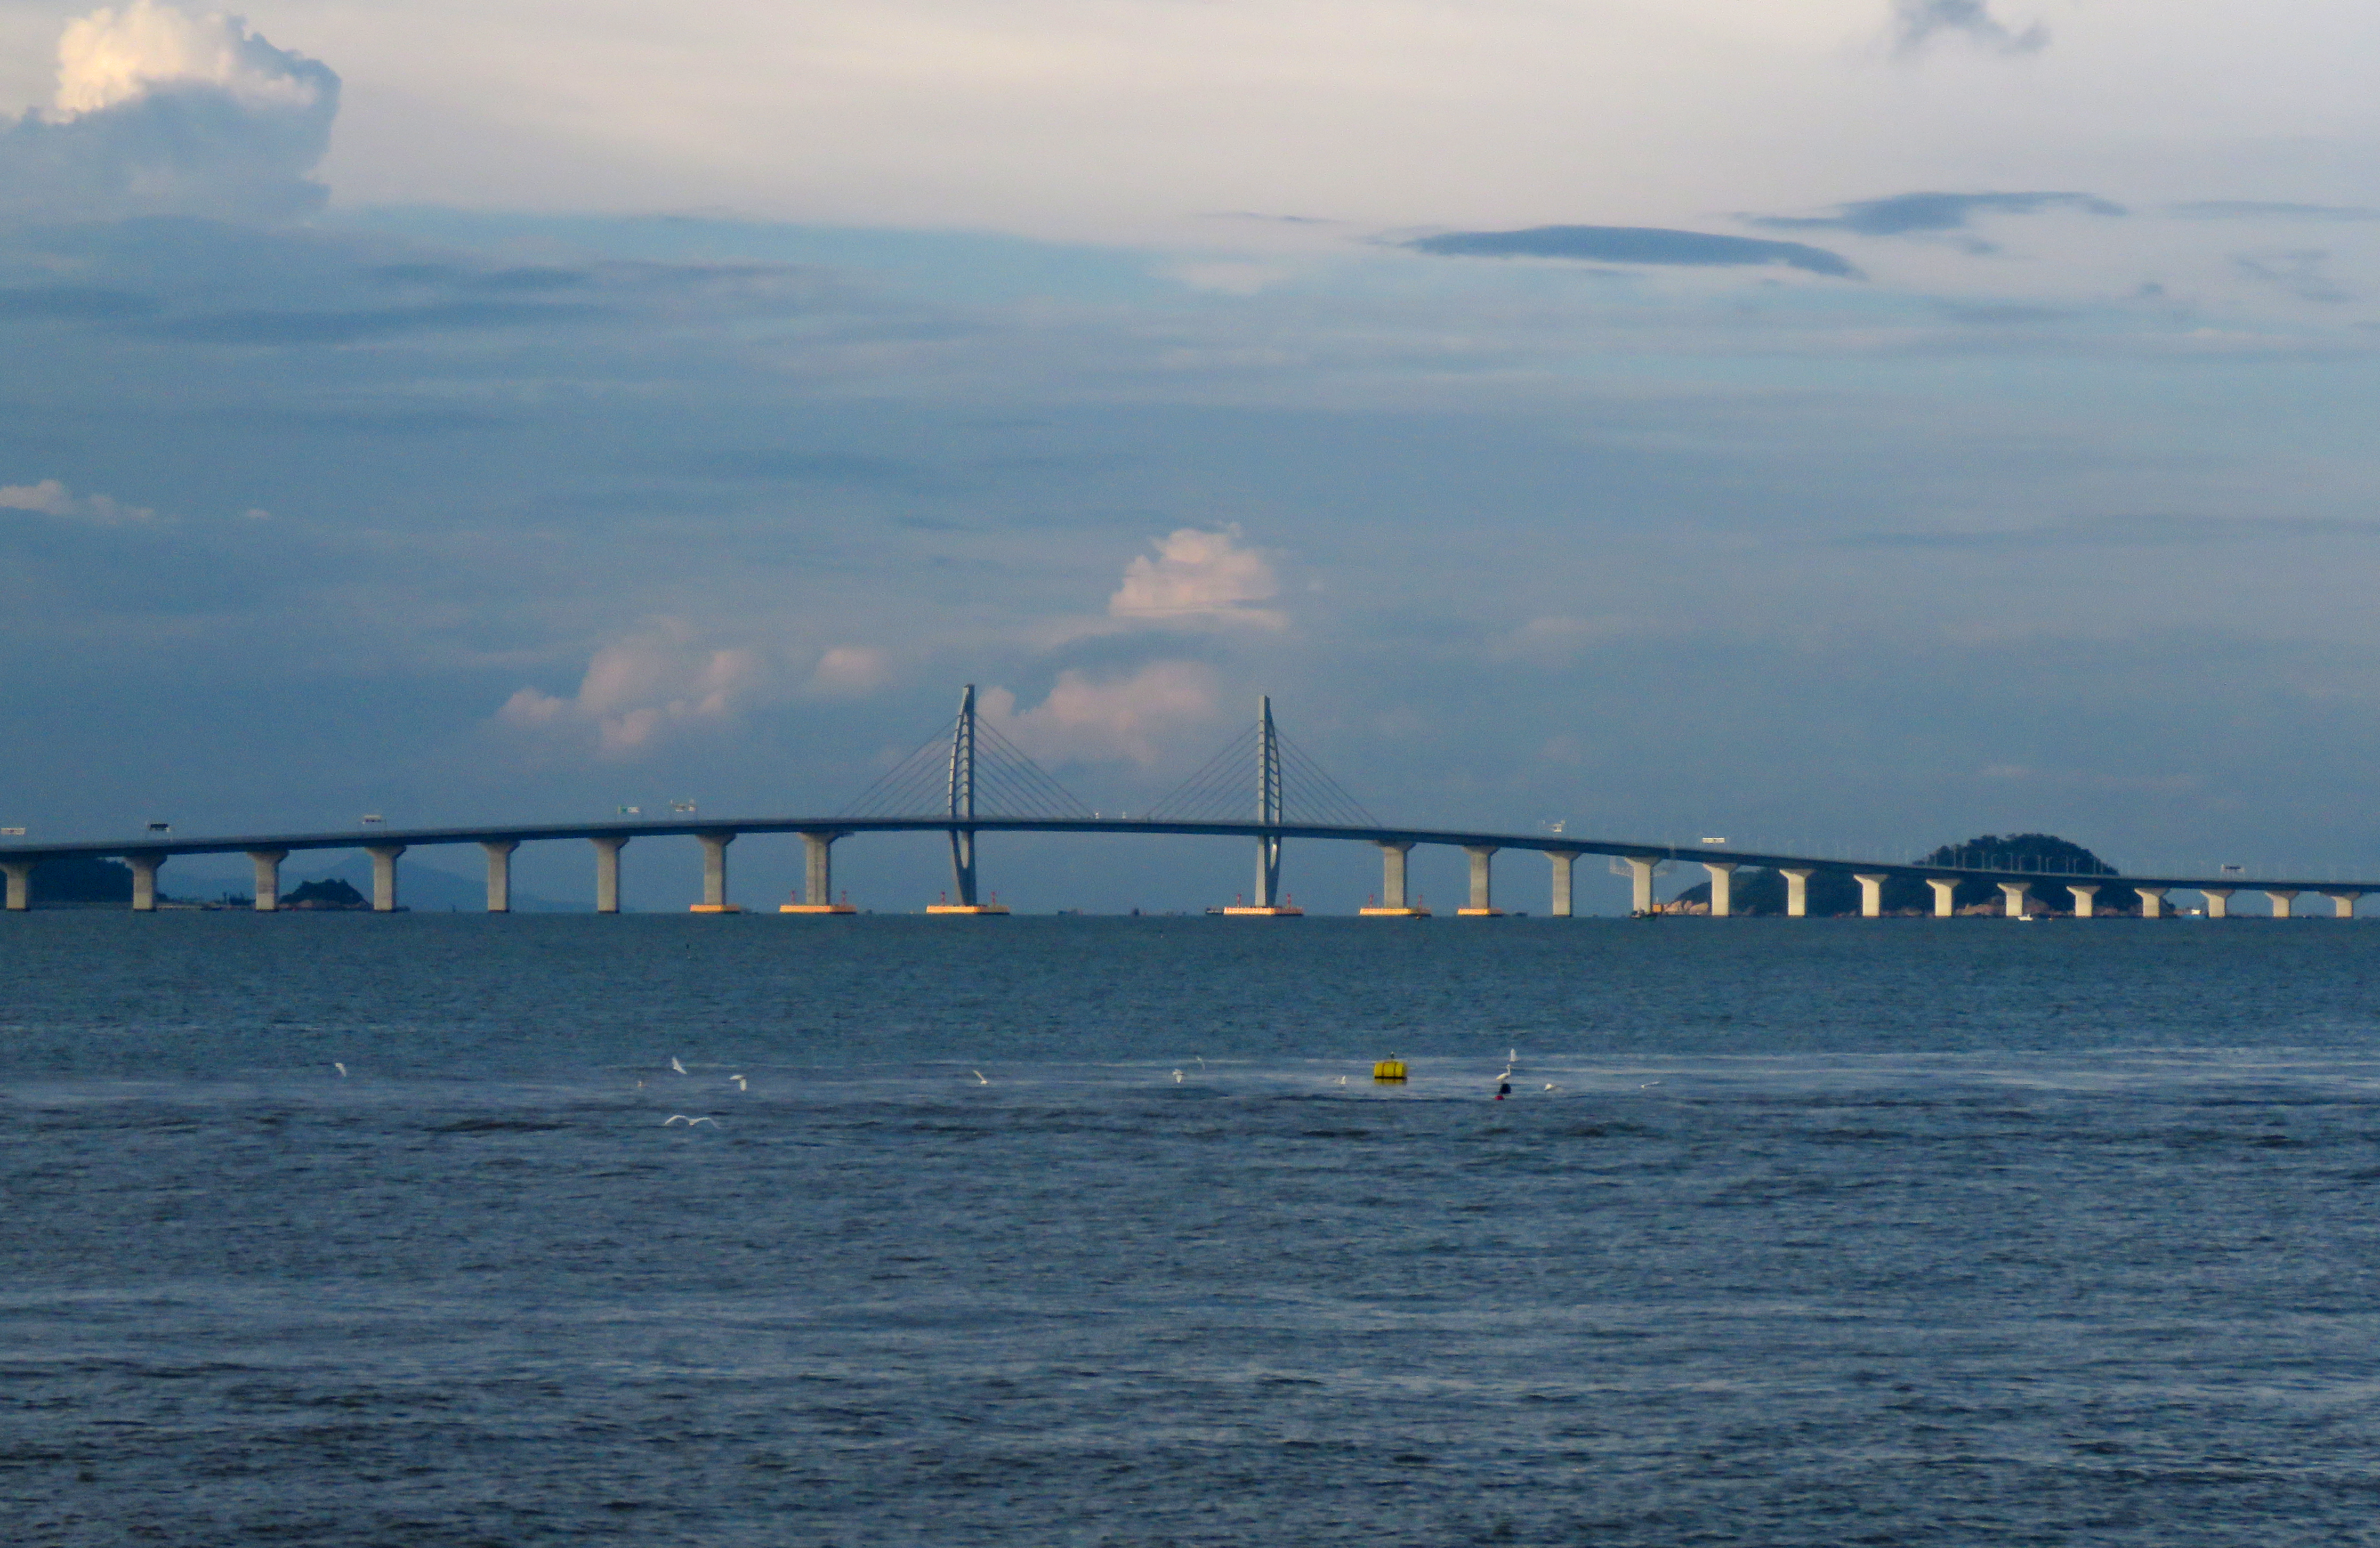
\includegraphics[width=.86\linewidth]{figures/chapter03/hzmb_west_section_N509FZ.jpg}%
}{摄影：N509FZ，2018年9月2日；Wikimedia Commons，CC BY-SA 4.0。照片未修改，仅按比例排印，来源与许可链接见文献\cite{hzmb-photo}。照片展示真实工程；以下数值均为教学自拟。}

\Needspace{8\baselineskip}
把复杂结构简化为三个沿同一方向移动的节点，两端固定，四段连接刚度都取1。记位移为 $\boldsymbol u$、外力为 $\boldsymbol f$，中间节点的平衡是 $(u_2-u_1)+(u_2-u_3)=f_2$；两侧节点同理：
\[
 K\boldsymbol u=\boldsymbol f,\qquad
 K=\OpMat{rrr}{2&-1&0\\-1&2&-1\\0&-1&2}=A.
\]
$K$ 是这个无量纲教学模型的\term{stiffness-matrix}，每种指定荷载是一个\term{load-case}。它与前面的 $A$ 完全相同，所以原来的 $L,U$ 可以直接使用；只需把 $\boldsymbol x,\boldsymbol b$ 分别读作位移 $\boldsymbol u$ 与荷载 $\boldsymbol f$。
\ThreeFigure{从真实桥梁的多工况问题，抽取一个可手算的三节点连接模型。}{fig:three-bridge-three-nodes}{%
\begin{tikzpicture}[x=1cm,y=1cm,font=\small]

\draw[very thick,ThreeGray] (.4,.4)--(.4,1.7) (11.6,.4)--(11.6,1.7);
\node[above] at (.4,1.8) {固定：$u_0=0$};
\node[above] at (11.6,1.8) {固定：$u_4=0$};
\draw[ThreeGray,thick] (0.40,1.00)--(0.85,1.00)--(0.95,1.15)--(1.15,0.85)--(1.35,1.15)--(1.55,0.85)--(1.75,1.15)--(1.95,0.85)--(2.15,1.15)--(2.35,0.85)--(2.55,1.15)--(2.75,1.00)--(3.20,1.00);
\node[] at (1.7999999999999998,0.25) {$k=1$};
\draw[ThreeGray,thick] (3.20,1.00)--(3.65,1.00)--(3.75,1.15)--(3.95,0.85)--(4.15,1.15)--(4.35,0.85)--(4.55,1.15)--(4.75,0.85)--(4.95,1.15)--(5.15,0.85)--(5.35,1.15)--(5.55,1.00)--(6.00,1.00);
\node[] at (4.6,0.25) {$k=1$};
\draw[ThreeGray,thick] (6.00,1.00)--(6.45,1.00)--(6.55,1.15)--(6.75,0.85)--(6.95,1.15)--(7.15,0.85)--(7.35,1.15)--(7.55,0.85)--(7.75,1.15)--(7.95,0.85)--(8.15,1.15)--(8.35,1.00)--(8.80,1.00);
\node[] at (7.4,0.25) {$k=1$};
\draw[ThreeGray,thick] (8.80,1.00)--(9.25,1.00)--(9.35,1.15)--(9.55,0.85)--(9.75,1.15)--(9.95,0.85)--(10.15,1.15)--(10.35,0.85)--(10.55,1.15)--(10.75,0.85)--(10.95,1.15)--(11.15,1.00)--(11.60,1.00);
\node[] at (10.2,0.25) {$k=1$};
\fill[ThreeBlue] (3.1999999999999997,1) circle (.13);
\node[] at (3.1999999999999997,1.75) {节点1：$u_1$};
\draw[oprose] (3.1999999999999997,-.3)--(4.199999999999999,-.3) node[right] {$f_1$};
\fill[ThreeBlue] (6.0,1) circle (.13);
\node[] at (6.0,1.75) {节点2：$u_2$};
\draw[oprose] (6.0,-.3)--(7.0,-.3) node[right] {$f_2$};
\fill[ThreeBlue] (8.799999999999999,1) circle (.13);
\node[] at (8.799999999999999,1.75) {节点3：$u_3$};
\draw[oprose] (8.799999999999999,-.3)--(9.799999999999999,-.3) node[right] {$f_3$};
\node[] at (6,-1.1) {所有位移与力均以向右为正；模型不按实桥比例绘制};
\end{tikzpicture}}{连接力取决于相对位移。例如中间节点的平衡为 $(u_2-u_1)+(u_2-u_3)=f_2$，所以系数自然成为 $-1,2,-1$。}

刚才算的就是节点1承受单位荷载。若把单位荷载移到节点2，\textbf{不用再计算任何消元乘数}，只将 $\boldsymbol f^{(2)}=(0,1,0)^{\mathrm T}$ 代入两次三角求解：
\[
 L\boldsymbol y=\boldsymbol f^{(2)}
 \ \Longrightarrow\ \boldsymbol y=(0,1,\tfrac23)^{\mathrm T},
 \qquad
 U\boldsymbol u^{(2)}=\boldsymbol y
 \ \Longrightarrow\ \boldsymbol u^{(2)}=(\tfrac12,1,\tfrac12)^{\mathrm T}.
\]
同理，荷载移到节点3时，$\boldsymbol y=(0,0,1)^{\mathrm T}$，解为 $\boldsymbol u^{(3)}=(\tfrac14,\tfrac12,\tfrac34)^{\mathrm T}$。三次计算的系数矩阵相同，分解也相同，改变的只有前代的输入及随后算出的数值。
\ThreeFigure{同一个连接模型，三种荷载位置，三组位移响应。}{fig:three-bridge-load-cases}{%
\begin{tikzpicture}[x=1cm,y=1cm,font=\small]
\node[] at (1.6,2.6) {工况1：荷载在节点1};
\node[] at (0.15,1.65) {$u_1$};
\fill[ThreeGray] (0.65,1.65) circle (.04);
\draw[opblue] (0.65,1.65)--(1.8125,1.65);
\node[] at (2.85,1.65) {$\frac34$};
\node[] at (0.15,0.9999999999999999) {$u_2$};
\fill[ThreeGray] (0.65,0.9999999999999999) circle (.04);
\draw[opblue] (0.65,0.9999999999999999)--(1.425,0.9999999999999999);
\node[] at (2.85,0.9999999999999999) {$\frac12$};
\node[] at (0.15,0.34999999999999987) {$u_3$};
\fill[ThreeGray] (0.65,0.34999999999999987) circle (.04);
\draw[opblue] (0.65,0.34999999999999987)--(1.0375,0.34999999999999987);
\node[] at (2.85,0.34999999999999987) {$\frac14$};
\node[] at (1.6,-0.4) {$(3/4,1/2,1/4)^{\mathrm T}$};
\node[] at (5.9,2.6) {工况2：荷载在节点2};
\node[] at (4.45,1.65) {$u_1$};
\fill[ThreeGray] (4.95,1.65) circle (.04);
\draw[opblue] (4.95,1.65)--(5.7250000000000005,1.65);
\node[] at (7.15,1.65) {$\frac12$};
\node[] at (4.45,0.9999999999999999) {$u_2$};
\fill[ThreeGray] (4.95,0.9999999999999999) circle (.04);
\draw[opblue] (4.95,0.9999999999999999)--(6.5,0.9999999999999999);
\node[] at (7.15,0.9999999999999999) {$1$};
\node[] at (4.45,0.34999999999999987) {$u_3$};
\fill[ThreeGray] (4.95,0.34999999999999987) circle (.04);
\draw[opblue] (4.95,0.34999999999999987)--(5.7250000000000005,0.34999999999999987);
\node[] at (7.15,0.34999999999999987) {$\frac12$};
\node[] at (5.9,-0.4) {$(1/2,1,1/2)^{\mathrm T}$};
\node[] at (10.2,2.6) {工况3：荷载在节点3};
\node[] at (8.75,1.65) {$u_1$};
\fill[ThreeGray] (9.25,1.65) circle (.04);
\draw[opblue] (9.25,1.65)--(9.6375,1.65);
\node[] at (11.45,1.65) {$\frac14$};
\node[] at (8.75,0.9999999999999999) {$u_2$};
\fill[ThreeGray] (9.25,0.9999999999999999) circle (.04);
\draw[opblue] (9.25,0.9999999999999999)--(10.025,0.9999999999999999);
\node[] at (11.45,0.9999999999999999) {$\frac12$};
\node[] at (8.75,0.34999999999999987) {$u_3$};
\fill[ThreeGray] (9.25,0.34999999999999987) circle (.04);
\draw[opblue] (9.25,0.34999999999999987)--(10.4125,0.34999999999999987);
\node[] at (11.45,0.34999999999999987) {$\frac34$};
\node[] at (10.2,-0.4) {$(1/4,1/2,3/4)^{\mathrm T}$};
\end{tikzpicture}}{每个工况中，三行依次对应三个节点。蓝色箭头长度与位移大小成比例，向右为正，与三节点模型的方向约定一致。}

\Needspace{5\baselineskip}
如果一次处理许多荷载，可以把它们并排成矩阵 $B$，把各组解并排成 $X$，就得到
\[
 AX=B\quad\Longrightarrow\quad LY=B\quad\Longrightarrow\quad UX=Y.
\]
每一列仍按同样的顺序求解。对一般稠密 $n$ 阶矩阵，分解的工作量大致随 $n^3$ 增长，每组前代与回代的工作量大致随 $n^2$ 增长；保存分解的收益，在右端项很多时尤其明显。通用数值库也将分解与随后求解组织为可分别调用的步骤\cite{lapack-linear}。对本例这种带状矩阵还可利用更多零元素减少计算，不能把稠密估计当成所有工程模型的精确成本。

同样的思路也适用于电路和导热：三个节点由四个单位电阻依次连接、两端接地时，节点电压满足 $K\boldsymbol v=\boldsymbol j$；均匀细杆取三个内部温度未知量、连接导热系数归一化为1时，相对于端点的温升满足 $K\boldsymbol t=\boldsymbol q$。这些都是教学简化模型；电路软件实际也会组织并求解矩阵系统\cite{ngspice-matrix}。固定元件或导热系数，改变输入，就能复用已经完成的分解。

\textbf{一次分解、多次求解的前提，是系数矩阵确实没有改变。}若材料刚度、连接方式或边界条件改变，就应重新检查并通常重新分解矩阵；不能只换右端项继续使用。对于本节固定的 $A$，无论 $\boldsymbol b$ 怎样改变，都按“先 $L\boldsymbol y=\boldsymbol b$，后 $U\boldsymbol x=\boldsymbol y$”重复求解。

我们现在可以把LU的意义连成一句话：\textbf{消元把方程组整理成三角形，$L$ 留下整理时的乘数，$U$ 留下整理后的系数；新问题沿着前代、回代两条路线就能得到解。}若消元中遇到零主元，或过小的主元使数值计算不稳，就需要改变行次序。下一节选读将用同一个桥梁模型说明PLU如何处理这件事。

\section{【选读】PLU分解：选主元与数值稳定性}
\label{sec:three-plu}

\textbf{本小节为拓展内容，不做考核要求。}主线中只要掌握LU怎样记录消元、怎样复用求解即可。本节进一步说明，计算机保存有限位数字时，为什么还要认真选择主元。


回到港珠澳大桥背景下的三节点教学模型。桥梁结构本身没有改变，但程序装配方程时，节点记录的读取次序可能不同。只要把方程和右端项一起重排，物理问题仍然相同；消元所见到的“第一个元素”却可能改变。因此，\textbf{固定结构值得复用分解，实际求解还要选择合适的主元顺序。}本节用重排后的同一个 $K$ 展示这一点，随后用小主元例子说明有限精度的影响。


考虑矩阵 $\OpMat{rr}{0&1\\1&1}$。它的映射可逆，但第1个位置为0，无法直接用它消去下方的1。交换两行后便可继续。这个例子说明：\textbf{可逆矩阵也未必能按原行次序进行无换行的LU消元。}

即使主元非零，过小的主元也可能产生过大的消元倍数，放大只保留有限位数字造成的\term{rounding-error}。这属于\term{numerical-stability}问题：算法应尽量避免把有限精度计算中的小误差放大成结果中的大偏差。

\begin{example}[一个过小的主元]
考虑
\[
 \begin{cases}10^{-4}x+y=1,\\x+y=2.\end{cases}
\]
精确解为 $x=1/(1-10^{-4})$、$y=(1-2\cdot10^{-4})/(1-10^{-4})$，两者都接近1。

若每步只保留3位有效数字，用第1行直接消元，需要减去它的 $10^4$ 倍。第2行变为 $-9999y=-9998$，舍入后却成为 $-10000y=-10000$，给出 $y=1$；代回第1行得到 $x=0$，偏差很大。

若先交换两行，消元倍数只有 $10^{-4}$，由 $(1-10^{-4})y=1-2\cdot10^{-4}$ 得到舍入结果 $y=1$，再由 $x+y=2$ 得到 $x=1$，更接近精确解。
\end{example}

常用的\term{partial-pivoting}是在第 $k$ 步，从\textbf{尚未处理的第 $k$ 行及其下方}寻找当前列绝对值最大的元素，把它所在行交换到主元行，再消元。这使该步用于消去下方元素的倍数绝对值不超过1。它通常能改善数值表现，但不是对所有矩阵都绝对无误差的保证。

一次行交换对应一个交换矩阵，多次交换合起来仍是\term{permutation-matrix}：它的每行、每列恰有一个1，其余元素为0，用来重新排列向量分量。把所有行交换汇总为 $P$，得到\term{plu-factorization}的常用写法
\[
 \boxed{PA=LU.}
\]
本书始终采用这个约定。写成 $A=P^{-1}LU$ 与它等价；不同资料对置换矩阵的命名可能相差一个逆。对置换矩阵，$P^{-1}=P^{\mathrm T}$。


\begin{example}[同一桥梁模型，先读入节点2的方程]
把 $K\boldsymbol u=\boldsymbol f$ 的前两条方程交换后，程序看到的矩阵和右端项变为
\[
 A=\begin{bmatrix}-1&2&-1\\2&-1&0\\0&-1&2\end{bmatrix},\qquad
 \boldsymbol b=(f_2,f_1,f_3)^{\mathrm T}.
\]
第1列的候选主元绝对值为 $1,2,0$。选择第2行的2，交换前两行，取
\[
 P=\begin{bmatrix}0&1&0\\1&0&0\\0&0&1\end{bmatrix},\qquad
 PA=K,\qquad P\boldsymbol b=\boldsymbol f.
\]
于是第3.7节保存的 $L,U$ 立即给出 $PA=LU$。第2轮中，剩余候选值为 $3/2,-1$，不再需要换行。
\end{example}

例如荷载在节点1时，读入的右端项为 $\boldsymbol b=(0,1,0)^{\mathrm T}$。同步换行后恢复 $P\boldsymbol b=(1,0,0)^{\mathrm T}$，解得的物理位移仍为 $(3/4,1/2,1/4)^{\mathrm T}$。\textbf{换的是方程的排列，不是节点的物理位置，也不是未知量的列次序。}

\ThreeFigure{从LU到PLU：给同一个工程模型选择更合适的消元顺序。}{fig:three-plu}{%
\begin{tikzpicture}[x=1cm,y=1cm,font=\small]
\fill[ThreeRose!20] (0.3,2.5) rectangle ++(0.55,-0.5);
\node[inner sep=1pt] at (0.575,2.25) {$-1$};
\fill[ThreeRose!20] (0.8500000000000001,2.5) rectangle ++(0.55,-0.5);
\node[inner sep=1pt] at (1.125,2.25) {$2$};
\fill[ThreeRose!20] (1.4000000000000001,2.5) rectangle ++(0.55,-0.5);
\node[inner sep=1pt] at (1.675,2.25) {$-1$};
\fill[ThreeBlue!20] (0.3,2.0) rectangle ++(0.55,-0.5);
\node[inner sep=1pt] at (0.575,1.75) {$2$};
\fill[ThreeBlue!20] (0.8500000000000001,2.0) rectangle ++(0.55,-0.5);
\node[inner sep=1pt] at (1.125,1.75) {$-1$};
\fill[ThreeBlue!20] (1.4000000000000001,2.0) rectangle ++(0.55,-0.5);
\node[inner sep=1pt] at (1.675,1.75) {$0$};
\fill[ThreeGray!5] (0.3,1.5) rectangle ++(0.55,-0.5);
\node[inner sep=1pt] at (0.575,1.25) {$0$};
\fill[ThreeGray!5] (0.8500000000000001,1.5) rectangle ++(0.55,-0.5);
\node[inner sep=1pt] at (1.125,1.25) {$-1$};
\fill[ThreeGray!5] (1.4000000000000001,1.5) rectangle ++(0.55,-0.5);
\node[inner sep=1pt] at (1.675,1.25) {$2$};
\draw[ThreeGray,line width=.65pt] (0.27,2.5) -- ++(-.10,0) -- ++(0,-1.5) -- ++(.10,0);
\draw[ThreeGray,line width=.65pt] (1.9800000000000002,2.5) -- ++(.10,0) -- ++(0,-1.5) -- ++(-.10,0);
\node[font=\small] at (1.125,2.9) {$A$};
\node[] at (1.5,3.6) {装配次序：2、1、3};
\fill[ThreeRose!20] (2.2,2.5) rectangle ++(0.55,-0.5);
\node[inner sep=1pt] at (2.475,2.25) {$0$};
\fill[ThreeBlue!20] (2.2,2.0) rectangle ++(0.55,-0.5);
\node[inner sep=1pt] at (2.475,1.75) {$1$};
\fill[ThreeGray!5] (2.2,1.5) rectangle ++(0.55,-0.5);
\node[inner sep=1pt] at (2.475,1.25) {$0$};
\draw[ThreeGray,line width=.65pt] (2.1700000000000004,2.5) -- ++(-.10,0) -- ++(0,-1.5) -- ++(.10,0);
\draw[ThreeGray,line width=.65pt] (2.78,2.5) -- ++(.10,0) -- ++(0,-1.5) -- ++(-.10,0);
\node[font=\small] at (2.475,2.9) {$\boldsymbol b$};
\draw[threearrow] (3.2,1.8)--node[above] {同乘 $P$}(5.25,1.8);
\fill[ThreeBlue!20] (5.8,2.5) rectangle ++(0.55,-0.5);
\node[inner sep=1pt] at (6.075,2.25) {$2$};
\fill[ThreeBlue!20] (6.35,2.5) rectangle ++(0.55,-0.5);
\node[inner sep=1pt] at (6.625,2.25) {$-1$};
\fill[ThreeBlue!20] (6.9,2.5) rectangle ++(0.55,-0.5);
\node[inner sep=1pt] at (7.175,2.25) {$0$};
\fill[ThreeRose!20] (5.8,2.0) rectangle ++(0.55,-0.5);
\node[inner sep=1pt] at (6.075,1.75) {$-1$};
\fill[ThreeRose!20] (6.35,2.0) rectangle ++(0.55,-0.5);
\node[inner sep=1pt] at (6.625,1.75) {$2$};
\fill[ThreeRose!20] (6.9,2.0) rectangle ++(0.55,-0.5);
\node[inner sep=1pt] at (7.175,1.75) {$-1$};
\fill[ThreeGray!5] (5.8,1.5) rectangle ++(0.55,-0.5);
\node[inner sep=1pt] at (6.075,1.25) {$0$};
\fill[ThreeGray!5] (6.35,1.5) rectangle ++(0.55,-0.5);
\node[inner sep=1pt] at (6.625,1.25) {$-1$};
\fill[ThreeGray!5] (6.9,1.5) rectangle ++(0.55,-0.5);
\node[inner sep=1pt] at (7.175,1.25) {$2$};
\draw[ThreeGray,line width=.65pt] (5.77,2.5) -- ++(-.10,0) -- ++(0,-1.5) -- ++(.10,0);
\draw[ThreeGray,line width=.65pt] (7.48,2.5) -- ++(.10,0) -- ++(0,-1.5) -- ++(-.10,0);
\node[font=\small] at (6.625,2.9) {$PA=K$};
\fill[ThreeBlue!20] (7.7,2.5) rectangle ++(0.55,-0.5);
\node[inner sep=1pt] at (7.9750000000000005,2.25) {$1$};
\fill[ThreeRose!20] (7.7,2.0) rectangle ++(0.55,-0.5);
\node[inner sep=1pt] at (7.9750000000000005,1.75) {$0$};
\fill[ThreeGray!5] (7.7,1.5) rectangle ++(0.55,-0.5);
\node[inner sep=1pt] at (7.9750000000000005,1.25) {$0$};
\draw[ThreeGray,line width=.65pt] (7.67,2.5) -- ++(-.10,0) -- ++(0,-1.5) -- ++(.10,0);
\draw[ThreeGray,line width=.65pt] (8.28,2.5) -- ++(.10,0) -- ++(0,-1.5) -- ++(-.10,0);
\node[font=\small] at (7.9750000000000005,2.9) {$P\boldsymbol b$};
\draw[threearrow] (8.7,1.8)--(9.7,1.8);
\node[align=center] at (11,1.8) {复用同一组\\$L,U$};
\node[] at (6,-0.1) {一条方程的系数与右端项必须作为一个整体移动};
\end{tikzpicture}}{蓝色行与其右端项始终成对移动，玫红色行亦然。本例选主元后回到上一节的 $K$，可以逐项核对分解和位移。}

\OpNote{本例只在开头换行。如果在后续消元步骤中交换行，$L$ 前面各列已经保存的对应行元素，也必须随之交换，才能始终保持 $PA=LU$。}


解 $A\boldsymbol x=\boldsymbol b$ 时，先把右端项按同样的顺序排列，解 $L\boldsymbol y=P\boldsymbol b$，再解 $U\boldsymbol x=\boldsymbol y$。若选主元时发现当前列剩余部分全为零，则不能继续除以这个主元，应按第2章的解判定处理，而不能把换行当作总能使矩阵可逆的办法。

处理一般矩阵的数值软件中，带部分选主元的LU是常见方案，例如LAPACK的 \textsf{DGETRF} 就采用换行选主元\cite{lapack-getrf}。无换行LU并非只适用于某一种矩阵。\term{strict-diagonal-dominance}条件
\[
 |A_{i,i}|>\sum_{j\ne i}|A_{i,j}|\qquad(i=1,\ldots,n)
\]
是保证无换行消元可以进行的一类充分条件，却不是必要条件。例如 $\OpMat{rr}{1&2\\1&3}$ 不满足这一条件，但减去第1行后主元为1，仍能顺利得到LU。实际算法还会结合矩阵的具体结构选择方案。

LU与PLU保存的是“怎样消元”的信息。下一节选读换一个问题：如果若干列本来就可以由少数核心列表示，能否把矩阵拆成“核心列”与“组合系数”两部分？这将把本章的矩阵分解与第1章的基、线性表示重新连接起来。

\section{【选读】列秩分解（CR分解）}
\label{sec:three-cr}

\textbf{本小节为拓展内容，不做考核要求。}这里仍只使用第1章向量组的秩、第2章的行化简和本章的矩阵乘法，不讨论下一章的映射结构定理。

设 $A$ 的秩为 $r>0$。从它的原列中选一组极大无关组，按次序排成矩阵 $C$。第2章已证明：可先看阶梯形的主元列号，再\textbf{返回原矩阵}取出这些列。其余每一列都能由 $C$ 的列唯一线性表示，把各列的表示系数也按列记录成矩阵 $R$，就得到
\[
 A=CR.
\]
从映射看，输入 $\boldsymbol x$ 先经过 $R$，被整理成 $r$ 个核心方向的组合系数；再经过 $C$，将这些系数组合为实际输出。分解来自这个复合过程。

\begin{definition}[列秩分解]
若 $A$ 是秩为 $r>0$ 的 $m\times n$ 矩阵，分解
\[
 \boxed{A=CR,\qquad C:m\times r,\qquad R:r\times n}
\]
中 $C$ 的 $r$ 列线性无关，$R$ 的 $r$ 行线性无关，则称为\term{cr-factorization}，简称CR分解。列向量全部无关称为\term{full-column-rank}；行向量全部无关称为\term{full-row-rank}。
\end{definition}

零矩阵无需寻找核心列。若允许空矩阵，也可令 $C$ 为 $m\times0$、$R$ 为 $0\times n$，按空和为零的约定写成 $A=CR$；后面的算例均取 $r>0$。

\subsection*{从行最简形读出组合系数}

把 $A$ 化为行最简形 $U$，设主元列号为 $k_1,\ldots,k_r$。取原矩阵的这些列组成 $C$，再取 $U$ 的前 $r$ 个非零行组成 $R$。为什么这些行恰好给出所需的系数？

在 $U$ 中，主元列的前 $r$ 个分量依次是标准基。于是第 $j$ 列前 $r$ 个元素本身，就是它关于主元列的组合系数。行变换保持\textbf{对应列之间的线性关系及其系数}，因此同样的系数也把原矩阵的第 $j$ 列表示为 $C$ 的各列之和。逐列写出，正好是 $A=CR$。

另外，$R$ 的第 $k_1,\ldots,k_r$ 列组成 $E_r$，所以它的 $r$ 行无关：若若干行的线性组合为零，只看这些列，就立即得到各个系数全为零。这说明上面的构造同时满足两个无关条件。

\OpNote{$C$ 必须由原矩阵的主元对应列构成，不能从行最简形中直接拿列来代替。行化简保留的是列之间的表示关系，不是各列的坐标。只有 $R$ 取自行最简形的非零行。}

\begin{example}[两条核心列，组织四条列向量]
取
\[
 A=\OpMat{rrrr}{1&2&0&1\\0&0&1&1\\1&2&1&2}.
\]
先后作 $r_3\leftarrow r_3-r_1$、$r_3\leftarrow r_3-r_2$，得到
\[
 A\ \sim\ \OpMat{rrrr}{1&2&0&1\\0&0&1&1\\0&0&1&1}
 \ \sim\ U=\OpMat{rrrr}{1&2&0&1\\0&0&1&1\\0&0&0&0}.
\]
这已是行最简形，主元在第1、3列，故 $r(A)=2$。返回原矩阵取列，并保留 $U$ 的非零行，得
\[
 C=\OpMat{rr}{1&0\\0&1\\1&1},\qquad
 R=\OpMat{rrrr}{1&2&0&1\\0&0&1&1}.
\]
于是
\[
 A=CR=\OpMat{rr}{1&0\\0&1\\1&1}
        \OpMat{rrrr}{1&2&0&1\\0&0&1&1}.
\]
逐列看，四组系数为 $(1,0)^{\mathrm T}$、$(2,0)^{\mathrm T}$、$(0,1)^{\mathrm T}$、$(1,1)^{\mathrm T}$，分别说明原列为 $\boldsymbol a_1$、$2\boldsymbol a_1$、$\boldsymbol a_3$、$\boldsymbol a_1+\boldsymbol a_3$，与原数表一致。
\end{example}


\subsection*{先看取列，再看重建}

把算例中的数表染成两种颜色，便能看清 $C$ 与 $R$ 各自保留了什么。$C$ 中的两条竖向色带来自\textbf{原矩阵}；$R$ 中的两条横向色带来自\textbf{行最简形}。不要把这两个来源混在一起。



\ThreeFigure{CR的两条取材路线：原矩阵给出方向，行最简形给出系数。}{fig:three-cr-extract}{%
\begin{tikzpicture}[x=1cm,y=1cm,font=\small]
\fill[ThreeBlue!25] (0.3,3.4) rectangle ++(0.55,-0.5);
\node[inner sep=1pt] at (0.575,3.15) {$1$};
\fill[ThreeGray!5] (0.8500000000000001,3.4) rectangle ++(0.55,-0.5);
\node[inner sep=1pt] at (1.125,3.15) {$2$};
\fill[ThreeRose!25] (1.4000000000000001,3.4) rectangle ++(0.55,-0.5);
\node[inner sep=1pt] at (1.675,3.15) {$0$};
\fill[ThreeGray!5] (1.9500000000000002,3.4) rectangle ++(0.55,-0.5);
\node[inner sep=1pt] at (2.225,3.15) {$1$};
\fill[ThreeBlue!25] (0.3,2.9) rectangle ++(0.55,-0.5);
\node[inner sep=1pt] at (0.575,2.65) {$0$};
\fill[ThreeGray!5] (0.8500000000000001,2.9) rectangle ++(0.55,-0.5);
\node[inner sep=1pt] at (1.125,2.65) {$0$};
\fill[ThreeRose!25] (1.4000000000000001,2.9) rectangle ++(0.55,-0.5);
\node[inner sep=1pt] at (1.675,2.65) {$1$};
\fill[ThreeGray!5] (1.9500000000000002,2.9) rectangle ++(0.55,-0.5);
\node[inner sep=1pt] at (2.225,2.65) {$1$};
\fill[ThreeBlue!25] (0.3,2.4) rectangle ++(0.55,-0.5);
\node[inner sep=1pt] at (0.575,2.15) {$1$};
\fill[ThreeGray!5] (0.8500000000000001,2.4) rectangle ++(0.55,-0.5);
\node[inner sep=1pt] at (1.125,2.15) {$2$};
\fill[ThreeRose!25] (1.4000000000000001,2.4) rectangle ++(0.55,-0.5);
\node[inner sep=1pt] at (1.675,2.15) {$1$};
\fill[ThreeGray!5] (1.9500000000000002,2.4) rectangle ++(0.55,-0.5);
\node[inner sep=1pt] at (2.225,2.15) {$2$};
\draw[ThreeGray,line width=.65pt] (0.27,3.4) -- ++(-.10,0) -- ++(0,-1.5) -- ++(.10,0);
\draw[ThreeGray,line width=.65pt] (2.53,3.4) -- ++(.10,0) -- ++(0,-1.5) -- ++(-.10,0);
\node[font=\small] at (1.4000000000000001,3.8) {原矩阵 $A$};
\draw[threearrow] (2.95,2.65)--node[above,font=\footnotesize] {取第1、3列}(5.2,2.65);
\fill[ThreeBlue!25] (5.8,3.4) rectangle ++(0.55,-0.5);
\node[inner sep=1pt] at (6.075,3.15) {$1$};
\fill[ThreeRose!25] (6.35,3.4) rectangle ++(0.55,-0.5);
\node[inner sep=1pt] at (6.625,3.15) {$0$};
\fill[ThreeBlue!25] (5.8,2.9) rectangle ++(0.55,-0.5);
\node[inner sep=1pt] at (6.075,2.65) {$0$};
\fill[ThreeRose!25] (6.35,2.9) rectangle ++(0.55,-0.5);
\node[inner sep=1pt] at (6.625,2.65) {$1$};
\fill[ThreeBlue!25] (5.8,2.4) rectangle ++(0.55,-0.5);
\node[inner sep=1pt] at (6.075,2.15) {$1$};
\fill[ThreeRose!25] (6.35,2.4) rectangle ++(0.55,-0.5);
\node[inner sep=1pt] at (6.625,2.15) {$1$};
\draw[ThreeGray,line width=.65pt] (5.77,3.4) -- ++(-.10,0) -- ++(0,-1.5) -- ++(.10,0);
\draw[ThreeGray,line width=.65pt] (6.930000000000001,3.4) -- ++(.10,0) -- ++(0,-1.5) -- ++(-.10,0);
\node[font=\small] at (6.35,3.8) {$C$：方向不变};
\draw[threearrow] (1.4,1.5)--node[right,font=\footnotesize] {行化简}(1.4,.3);
\fill[ThreeBlue!18] (0.3,-0.2) rectangle ++(0.55,-0.5);
\node[inner sep=1pt] at (0.575,-0.45) {$1$};
\fill[ThreeBlue!18] (0.8500000000000001,-0.2) rectangle ++(0.55,-0.5);
\node[inner sep=1pt] at (1.125,-0.45) {$2$};
\fill[ThreeBlue!18] (1.4000000000000001,-0.2) rectangle ++(0.55,-0.5);
\node[inner sep=1pt] at (1.675,-0.45) {$0$};
\fill[ThreeBlue!18] (1.9500000000000002,-0.2) rectangle ++(0.55,-0.5);
\node[inner sep=1pt] at (2.225,-0.45) {$1$};
\fill[ThreeRose!18] (0.3,-0.7) rectangle ++(0.55,-0.5);
\node[inner sep=1pt] at (0.575,-0.95) {$0$};
\fill[ThreeRose!18] (0.8500000000000001,-0.7) rectangle ++(0.55,-0.5);
\node[inner sep=1pt] at (1.125,-0.95) {$0$};
\fill[ThreeRose!18] (1.4000000000000001,-0.7) rectangle ++(0.55,-0.5);
\node[inner sep=1pt] at (1.675,-0.95) {$1$};
\fill[ThreeRose!18] (1.9500000000000002,-0.7) rectangle ++(0.55,-0.5);
\node[inner sep=1pt] at (2.225,-0.95) {$1$};
\fill[ThreeGray!5] (0.3,-1.2) rectangle ++(0.55,-0.5);
\node[inner sep=1pt] at (0.575,-1.45) {$0$};
\fill[ThreeGray!5] (0.8500000000000001,-1.2) rectangle ++(0.55,-0.5);
\node[inner sep=1pt] at (1.125,-1.45) {$0$};
\fill[ThreeGray!5] (1.4000000000000001,-1.2) rectangle ++(0.55,-0.5);
\node[inner sep=1pt] at (1.675,-1.45) {$0$};
\fill[ThreeGray!5] (1.9500000000000002,-1.2) rectangle ++(0.55,-0.5);
\node[inner sep=1pt] at (2.225,-1.45) {$0$};
\draw[ThreeGray,line width=.65pt] (0.27,-0.2) -- ++(-.10,0) -- ++(0,-1.5) -- ++(.10,0);
\draw[ThreeGray,line width=.65pt] (2.53,-0.2) -- ++(.10,0) -- ++(0,-1.5) -- ++(-.10,0);
\node[font=\small] at (1.4000000000000001,0.2) {行最简形};
\draw[threearrow] (2.95,-.95)--node[above,font=\footnotesize] {去掉零行}(5.2,-.95);
\fill[ThreeBlue!18] (5.8,-0.2) rectangle ++(0.55,-0.5);
\node[inner sep=1pt] at (6.075,-0.45) {$1$};
\fill[ThreeBlue!18] (6.35,-0.2) rectangle ++(0.55,-0.5);
\node[inner sep=1pt] at (6.625,-0.45) {$2$};
\fill[ThreeBlue!18] (6.9,-0.2) rectangle ++(0.55,-0.5);
\node[inner sep=1pt] at (7.175,-0.45) {$0$};
\fill[ThreeBlue!18] (7.45,-0.2) rectangle ++(0.55,-0.5);
\node[inner sep=1pt] at (7.725,-0.45) {$1$};
\fill[ThreeRose!18] (5.8,-0.7) rectangle ++(0.55,-0.5);
\node[inner sep=1pt] at (6.075,-0.95) {$0$};
\fill[ThreeRose!18] (6.35,-0.7) rectangle ++(0.55,-0.5);
\node[inner sep=1pt] at (6.625,-0.95) {$0$};
\fill[ThreeRose!18] (6.9,-0.7) rectangle ++(0.55,-0.5);
\node[inner sep=1pt] at (7.175,-0.95) {$1$};
\fill[ThreeRose!18] (7.45,-0.7) rectangle ++(0.55,-0.5);
\node[inner sep=1pt] at (7.725,-0.95) {$1$};
\draw[ThreeGray,line width=.65pt] (5.77,-0.2) -- ++(-.10,0) -- ++(0,-1.0) -- ++(.10,0);
\draw[ThreeGray,line width=.65pt] (8.03,-0.2) -- ++(.10,0) -- ++(0,-1.0) -- ++(-.10,0);
\node[font=\small] at (6.9,0.2) {$R$：组合系数};
\node[font=\Large] at (10,1.4) {$A=CR$};
\node[align=center] at (10,0.1) {取列认原表\\取系数看化简};
\end{tikzpicture}}{行化简后的第1、3列只负责提示主元位置；真正放进 $C$ 的仍是原矩阵的第1、3列。}

\ThreeFigure{逐列重建：$R$ 的每一列都是一张“两种方向如何配比”的记录。}{fig:three-cr-columns}{%
\begin{tikzpicture}[x=1cm,y=1cm,font=\small]
\fill[ThreeGreen!15] (0.3,2.8) rectangle ++(0.55,-0.5);
\node[inner sep=1pt] at (0.575,2.55) {$1$};
\fill[ThreeGreen!15] (0.3,2.3) rectangle ++(0.55,-0.5);
\node[inner sep=1pt] at (0.575,2.05) {$0$};
\fill[ThreeGreen!15] (0.3,1.7999999999999998) rectangle ++(0.55,-0.5);
\node[inner sep=1pt] at (0.575,1.5499999999999998) {$1$};
\draw[ThreeGray,line width=.65pt] (0.27,2.8) -- ++(-.10,0) -- ++(0,-1.5) -- ++(.10,0);
\draw[ThreeGray,line width=.65pt] (0.8800000000000001,2.8) -- ++(.10,0) -- ++(0,-1.5) -- ++(-.10,0);
\node[font=\small] at (0.575,3.1999999999999997) {第1列};
\node[] at (1.35,2.05) {$\leftarrow$};
\node[] at (1.1,0.65) {$\boldsymbol c_1$};
\fill[ThreeBlue!22] (1.8,2.55) rectangle ++(0.55,-0.5);
\node[inner sep=1pt] at (2.075,2.3) {$1$};
\fill[ThreeRose!22] (1.8,2.05) rectangle ++(0.55,-0.5);
\node[inner sep=1pt] at (2.075,1.7999999999999998) {$0$};
\draw[ThreeGray,line width=.65pt] (1.77,2.55) -- ++(-.10,0) -- ++(0,-1.0) -- ++(.10,0);
\draw[ThreeGray,line width=.65pt] (2.38,2.55) -- ++(.10,0) -- ++(0,-1.0) -- ++(-.10,0);
\fill[ThreeGreen!15] (3.3,2.8) rectangle ++(0.55,-0.5);
\node[inner sep=1pt] at (3.5749999999999997,2.55) {$2$};
\fill[ThreeGreen!15] (3.3,2.3) rectangle ++(0.55,-0.5);
\node[inner sep=1pt] at (3.5749999999999997,2.05) {$0$};
\fill[ThreeGreen!15] (3.3,1.7999999999999998) rectangle ++(0.55,-0.5);
\node[inner sep=1pt] at (3.5749999999999997,1.5499999999999998) {$2$};
\draw[ThreeGray,line width=.65pt] (3.27,2.8) -- ++(-.10,0) -- ++(0,-1.5) -- ++(.10,0);
\draw[ThreeGray,line width=.65pt] (3.8799999999999994,2.8) -- ++(.10,0) -- ++(0,-1.5) -- ++(-.10,0);
\node[font=\small] at (3.5749999999999997,3.1999999999999997) {第2列};
\node[] at (4.35,2.05) {$\leftarrow$};
\node[] at (4.1,0.65) {$2\boldsymbol c_1$};
\fill[ThreeBlue!22] (4.8,2.55) rectangle ++(0.55,-0.5);
\node[inner sep=1pt] at (5.075,2.3) {$2$};
\fill[ThreeRose!22] (4.8,2.05) rectangle ++(0.55,-0.5);
\node[inner sep=1pt] at (5.075,1.7999999999999998) {$0$};
\draw[ThreeGray,line width=.65pt] (4.77,2.55) -- ++(-.10,0) -- ++(0,-1.0) -- ++(.10,0);
\draw[ThreeGray,line width=.65pt] (5.38,2.55) -- ++(.10,0) -- ++(0,-1.0) -- ++(-.10,0);
\fill[ThreeGreen!15] (6.3,2.8) rectangle ++(0.55,-0.5);
\node[inner sep=1pt] at (6.575,2.55) {$0$};
\fill[ThreeGreen!15] (6.3,2.3) rectangle ++(0.55,-0.5);
\node[inner sep=1pt] at (6.575,2.05) {$1$};
\fill[ThreeGreen!15] (6.3,1.7999999999999998) rectangle ++(0.55,-0.5);
\node[inner sep=1pt] at (6.575,1.5499999999999998) {$1$};
\draw[ThreeGray,line width=.65pt] (6.27,2.8) -- ++(-.10,0) -- ++(0,-1.5) -- ++(.10,0);
\draw[ThreeGray,line width=.65pt] (6.88,2.8) -- ++(.10,0) -- ++(0,-1.5) -- ++(-.10,0);
\node[font=\small] at (6.575,3.1999999999999997) {第3列};
\node[] at (7.35,2.05) {$\leftarrow$};
\node[] at (7.1,0.65) {$\boldsymbol c_2$};
\fill[ThreeBlue!22] (7.8,2.55) rectangle ++(0.55,-0.5);
\node[inner sep=1pt] at (8.075,2.3) {$0$};
\fill[ThreeRose!22] (7.8,2.05) rectangle ++(0.55,-0.5);
\node[inner sep=1pt] at (8.075,1.7999999999999998) {$1$};
\draw[ThreeGray,line width=.65pt] (7.77,2.55) -- ++(-.10,0) -- ++(0,-1.0) -- ++(.10,0);
\draw[ThreeGray,line width=.65pt] (8.379999999999999,2.55) -- ++(.10,0) -- ++(0,-1.0) -- ++(-.10,0);
\fill[ThreeGreen!15] (9.3,2.8) rectangle ++(0.55,-0.5);
\node[inner sep=1pt] at (9.575000000000001,2.55) {$1$};
\fill[ThreeGreen!15] (9.3,2.3) rectangle ++(0.55,-0.5);
\node[inner sep=1pt] at (9.575000000000001,2.05) {$1$};
\fill[ThreeGreen!15] (9.3,1.7999999999999998) rectangle ++(0.55,-0.5);
\node[inner sep=1pt] at (9.575000000000001,1.5499999999999998) {$2$};
\draw[ThreeGray,line width=.65pt] (9.270000000000001,2.8) -- ++(-.10,0) -- ++(0,-1.5) -- ++(.10,0);
\draw[ThreeGray,line width=.65pt] (9.88,2.8) -- ++(.10,0) -- ++(0,-1.5) -- ++(-.10,0);
\node[font=\small] at (9.575000000000001,3.1999999999999997) {第4列};
\node[] at (10.350000000000001,2.05) {$\leftarrow$};
\node[] at (10.100000000000001,0.65) {$\boldsymbol c_1+\boldsymbol c_2$};
\fill[ThreeBlue!22] (10.8,2.55) rectangle ++(0.55,-0.5);
\node[inner sep=1pt] at (11.075000000000001,2.3) {$1$};
\fill[ThreeRose!22] (10.8,2.05) rectangle ++(0.55,-0.5);
\node[inner sep=1pt] at (11.075000000000001,1.7999999999999998) {$1$};
\draw[ThreeGray,line width=.65pt] (10.770000000000001,2.55) -- ++(-.10,0) -- ++(0,-1.0) -- ++(.10,0);
\draw[ThreeGray,line width=.65pt] (11.38,2.55) -- ++(.10,0) -- ++(0,-1.0) -- ++(-.10,0);
\node[] at (5.8,-0.2) {右侧两格是 $R$ 的对应列：上格乘 $\boldsymbol c_1$，下格乘 $\boldsymbol c_2$};
\end{tikzpicture}}{例如最后一列的系数为 $(1,1)^{\mathrm T}$，因此原矩阵最后一列是两个核心列之和。}

也可以采用第3.3节的外积视角，把两条核心列各自的贡献铺成整张数表：
\[
 A=\boldsymbol c_1[\,1\quad2\quad0\quad1\,]
   +\boldsymbol c_2[\,0\quad0\quad1\quad1\,].
\]

\ThreeFigure{两张外积数表叠加，恢复整个矩阵。}{fig:three-cr-outer}{%
\begin{tikzpicture}[x=1cm,y=1cm,font=\small]
\fill[ThreeBlue!18] (0.25,2.1) rectangle ++(0.49,-0.5);
\node[inner sep=1pt] at (0.495,1.85) {$1$};
\fill[ThreeBlue!18] (0.74,2.1) rectangle ++(0.49,-0.5);
\node[inner sep=1pt] at (0.985,1.85) {$2$};
\fill[ThreeBlue!18] (1.23,2.1) rectangle ++(0.49,-0.5);
\node[inner sep=1pt] at (1.475,1.85) {$0$};
\fill[ThreeBlue!18] (1.72,2.1) rectangle ++(0.49,-0.5);
\node[inner sep=1pt] at (1.9649999999999999,1.85) {$1$};
\fill[ThreeBlue!18] (0.25,1.6) rectangle ++(0.49,-0.5);
\node[inner sep=1pt] at (0.495,1.35) {$0$};
\fill[ThreeBlue!18] (0.74,1.6) rectangle ++(0.49,-0.5);
\node[inner sep=1pt] at (0.985,1.35) {$0$};
\fill[ThreeBlue!18] (1.23,1.6) rectangle ++(0.49,-0.5);
\node[inner sep=1pt] at (1.475,1.35) {$0$};
\fill[ThreeBlue!18] (1.72,1.6) rectangle ++(0.49,-0.5);
\node[inner sep=1pt] at (1.9649999999999999,1.35) {$0$};
\fill[ThreeBlue!18] (0.25,1.1) rectangle ++(0.49,-0.5);
\node[inner sep=1pt] at (0.495,0.8500000000000001) {$1$};
\fill[ThreeBlue!18] (0.74,1.1) rectangle ++(0.49,-0.5);
\node[inner sep=1pt] at (0.985,0.8500000000000001) {$2$};
\fill[ThreeBlue!18] (1.23,1.1) rectangle ++(0.49,-0.5);
\node[inner sep=1pt] at (1.475,0.8500000000000001) {$0$};
\fill[ThreeBlue!18] (1.72,1.1) rectangle ++(0.49,-0.5);
\node[inner sep=1pt] at (1.9649999999999999,0.8500000000000001) {$1$};
\draw[ThreeGray,line width=.65pt] (0.22,2.1) -- ++(-.10,0) -- ++(0,-1.5) -- ++(.10,0);
\draw[ThreeGray,line width=.65pt] (2.2399999999999998,2.1) -- ++(.10,0) -- ++(0,-1.5) -- ++(-.10,0);
\node[font=\small] at (1.23,2.5) {方向1的贡献};
\node[] at (2.85,1.35) {$+$};
\fill[ThreeRose!18] (3.45,2.1) rectangle ++(0.49,-0.5);
\node[inner sep=1pt] at (3.6950000000000003,1.85) {$0$};
\fill[ThreeRose!18] (3.9400000000000004,2.1) rectangle ++(0.49,-0.5);
\node[inner sep=1pt] at (4.1850000000000005,1.85) {$0$};
\fill[ThreeRose!18] (4.43,2.1) rectangle ++(0.49,-0.5);
\node[inner sep=1pt] at (4.675000000000001,1.85) {$0$};
\fill[ThreeRose!18] (4.92,2.1) rectangle ++(0.49,-0.5);
\node[inner sep=1pt] at (5.165,1.85) {$0$};
\fill[ThreeRose!18] (3.45,1.6) rectangle ++(0.49,-0.5);
\node[inner sep=1pt] at (3.6950000000000003,1.35) {$0$};
\fill[ThreeRose!18] (3.9400000000000004,1.6) rectangle ++(0.49,-0.5);
\node[inner sep=1pt] at (4.1850000000000005,1.35) {$0$};
\fill[ThreeRose!18] (4.43,1.6) rectangle ++(0.49,-0.5);
\node[inner sep=1pt] at (4.675000000000001,1.35) {$1$};
\fill[ThreeRose!18] (4.92,1.6) rectangle ++(0.49,-0.5);
\node[inner sep=1pt] at (5.165,1.35) {$1$};
\fill[ThreeRose!18] (3.45,1.1) rectangle ++(0.49,-0.5);
\node[inner sep=1pt] at (3.6950000000000003,0.8500000000000001) {$0$};
\fill[ThreeRose!18] (3.9400000000000004,1.1) rectangle ++(0.49,-0.5);
\node[inner sep=1pt] at (4.1850000000000005,0.8500000000000001) {$0$};
\fill[ThreeRose!18] (4.43,1.1) rectangle ++(0.49,-0.5);
\node[inner sep=1pt] at (4.675000000000001,0.8500000000000001) {$1$};
\fill[ThreeRose!18] (4.92,1.1) rectangle ++(0.49,-0.5);
\node[inner sep=1pt] at (5.165,0.8500000000000001) {$1$};
\draw[ThreeGray,line width=.65pt] (3.4200000000000004,2.1) -- ++(-.10,0) -- ++(0,-1.5) -- ++(.10,0);
\draw[ThreeGray,line width=.65pt] (5.44,2.1) -- ++(.10,0) -- ++(0,-1.5) -- ++(-.10,0);
\node[font=\small] at (4.43,2.5) {方向2的贡献};
\node[] at (6.05,1.35) {$=$};
\fill[ThreeGreen!16] (6.65,2.1) rectangle ++(0.49,-0.5);
\node[inner sep=1pt] at (6.8950000000000005,1.85) {$1$};
\fill[ThreeGreen!16] (7.140000000000001,2.1) rectangle ++(0.49,-0.5);
\node[inner sep=1pt] at (7.385000000000001,1.85) {$2$};
\fill[ThreeGreen!16] (7.630000000000001,2.1) rectangle ++(0.49,-0.5);
\node[inner sep=1pt] at (7.875,1.85) {$0$};
\fill[ThreeGreen!16] (8.120000000000001,2.1) rectangle ++(0.49,-0.5);
\node[inner sep=1pt] at (8.365,1.85) {$1$};
\fill[ThreeGreen!16] (6.65,1.6) rectangle ++(0.49,-0.5);
\node[inner sep=1pt] at (6.8950000000000005,1.35) {$0$};
\fill[ThreeGreen!16] (7.140000000000001,1.6) rectangle ++(0.49,-0.5);
\node[inner sep=1pt] at (7.385000000000001,1.35) {$0$};
\fill[ThreeGreen!16] (7.630000000000001,1.6) rectangle ++(0.49,-0.5);
\node[inner sep=1pt] at (7.875,1.35) {$1$};
\fill[ThreeGreen!16] (8.120000000000001,1.6) rectangle ++(0.49,-0.5);
\node[inner sep=1pt] at (8.365,1.35) {$1$};
\fill[ThreeGreen!16] (6.65,1.1) rectangle ++(0.49,-0.5);
\node[inner sep=1pt] at (6.8950000000000005,0.8500000000000001) {$1$};
\fill[ThreeGreen!16] (7.140000000000001,1.1) rectangle ++(0.49,-0.5);
\node[inner sep=1pt] at (7.385000000000001,0.8500000000000001) {$2$};
\fill[ThreeGreen!16] (7.630000000000001,1.1) rectangle ++(0.49,-0.5);
\node[inner sep=1pt] at (7.875,0.8500000000000001) {$1$};
\fill[ThreeGreen!16] (8.120000000000001,1.1) rectangle ++(0.49,-0.5);
\node[inner sep=1pt] at (8.365,0.8500000000000001) {$2$};
\draw[ThreeGray,line width=.65pt] (6.62,2.1) -- ++(-.10,0) -- ++(0,-1.5) -- ++(.10,0);
\draw[ThreeGray,line width=.65pt] (8.639999999999999,2.1) -- ++(.10,0) -- ++(0,-1.5) -- ++(-.10,0);
\node[font=\small] at (7.630000000000001,2.5) {$A$};
\end{tikzpicture}}{LU的每一块记录一次消元贡献；CR的每一块记录一个核心列方向的贡献。二者都通过“列乘行、再求和”恢复原矩阵。}


\ThreeFigure{CR分解先提取核心方向的组合系数，再把系数还原为输出。例题中两个核心列张成三维空间内的平面 $z=x+y$。}{fig:three-cr-geometry}{%
\begin{tikzpicture}[font=\footnotesize,x=1cm,y=1cm]
 \node[align=center] (x) at (.6,2.25) {输入\\$\boldsymbol x\in\mathbb R^4$};
 \node[threecard,fill=ThreeBlue!7,minimum width=1.5cm,minimum height=.8cm] (r) at (3.0,2.25) {$R$};
 \node[align=center] (t) at (5.65,2.25) {核心系数\\$(s,t)^{\mathrm T}\in\mathbb R^2$};
 \node[threecard,fill=ThreeRose!7,minimum width=1.5cm,minimum height=.8cm] (c) at (8.25,2.25) {$C$};
 \draw[threearrow] (x)--(r);\draw[threearrow] (r)--(t);\draw[threearrow] (t)--(c);
 \draw[threearrow] (c.east)--(9.6,2.25);
 \begin{scope}[shift={(11,1.05)},x={(-.65cm,-.35cm)},y={(.85cm,-.15cm)},z={(0cm,1cm)}]
  \fill[ThreeGreen!12] (0,0,0)--(1.7,0,1.7)--(1.7,1.7,3.4)--(0,1.7,1.7)--cycle;
  \draw[opaxis] (0,0,0)--(2,0,0) node[below] {$x$};
  \draw[opaxis] (0,0,0)--(0,2.1,0) node[right] {$y$};
  \draw[opaxis] (0,0,0)--(0,0,2.6) node[above] {$z$};
  \draw[opblue] (0,0,0)--(1,0,1) node[left] {$\boldsymbol a_1$};
  \draw[oprose] (0,0,0)--(0,1,1) node[right] {$\boldsymbol a_3$};
 \end{scope}
 \node[align=center] at (6.2,-.1)
  {$R\boldsymbol x=(x_1+2x_2+x_4,\ x_3+x_4)^{\mathrm T}=(s,t)^{\mathrm T}$\\[5pt]
   $C(s,t)^{\mathrm T}=s\boldsymbol a_1+t\boldsymbol a_3=(s,t,s+t)^{\mathrm T}$};
\end{tikzpicture}}{四个输入分量先变成两个组合系数，再变成三个输出分量。$C$ 保留核心方向，$R$ 保存各原列如何由核心列组成，二者各自记录不同的信息。}

第3.5节已经从转置引入列空间与行空间：它们分别由矩阵的列与行张成，分别位于 $\mathbb R^m$ 与 $\mathbb R^n$，不应混在一起。在本节的构造中，$C$ 与 $A$ 的列空间相同：$C$ 的列取自 $A$，而 $A$ 的每列又由 $C$ 的列表示。$R$ 与 $A$ 的行空间也相同：可逆的行变换不改变各行能够张成的范围，去掉零行也不改变它。

因此，CR分解没有把一个矩阵任意切成两块，而是把“可用的输出方向”与“生成这些输出的系数关系”分开记录。核心列可以有不同的选择，所以分解一般不唯一；按行最简形的主元列来选取，是一种明确且便于计算的办法。


\subsection*{回到桥梁：四种荷载，只解两种核心工况}

沿用第3.7节的连接矩阵 $K$，现在考虑一个含四种荷载的教学资料库：外侧两节点同时受力、该荷载加倍、右侧两节点同时受力，以及两种基本荷载叠加。把四个荷载向量并排放入 $F$，恰好得到刚才的数表：
\[
 F=\begin{bmatrix}1&2&0&1\\0&0&1&1\\1&2&1&2\end{bmatrix}=CR.
\]
这里 $C$ 记录两种独立荷载图样，$R$ 记录每种工况如何组合。\textbf{这只是本例选定的荷载库具有秩2，并不表示真实桥梁只需要检查两种荷载。}

用已保存的LU或PLU分解，只求两组核心响应 $K\boldsymbol u_{c_1}=\boldsymbol c_1$、$K\boldsymbol u_{c_2}=\boldsymbol c_2$，得到
\[
 U_C=[\,\boldsymbol u_{c_1}\quad\boldsymbol u_{c_2}\,]
 =\begin{bmatrix}1&3/4\\1&3/2\\1&5/4\end{bmatrix}.
\]
全部四组位移可以直接组合为 $X=U_CR$。因为
\[
 KX=K(U_CR)=(KU_C)R=CR=F,
\]
所以第二组响应是第一组的2倍，第四组响应是两组核心响应之和。这是线性叠加与矩阵结合律的直接应用。

\ThreeFigure{从CR的列关系，读出工程工况之间的组合关系。}{fig:three-cr-bridge-loads}{%
\begin{tikzpicture}[x=1cm,y=1cm,font=\small]
\node[] at (1.3,2.4) {工况1};
\draw[ThreeGray,thick] (0.0,.6)--(2.6,.6);
\fill[ThreeGray] (0.5,.6) circle (.05);
\draw[opguide] (0.5,.6)--(0.5,1.1);
\draw[oprose] (0.5,1.1)--(0.77,1.1);
\node[] at (0.635,1.55) {$1$};
\fill[ThreeGray] (1.3,.6) circle (.05);
\fill[ThreeGray] (2.1,.6) circle (.05);
\draw[opguide] (2.1,.6)--(2.1,1.1);
\draw[oprose] (2.1,1.1)--(2.37,1.1);
\node[] at (2.2350000000000003,1.55) {$1$};
\node[] at (1.3,0.15) {$\boldsymbol c_1$};
\node[] at (4.6,2.4) {工况2};
\draw[ThreeGray,thick] (3.3,.6)--(5.9,.6);
\fill[ThreeGray] (3.8,.6) circle (.05);
\draw[opguide] (3.8,.6)--(3.8,1.1);
\draw[oprose] (3.8,1.1)--(4.34,1.1);
\node[] at (4.07,1.55) {$2$};
\fill[ThreeGray] (4.6,.6) circle (.05);
\fill[ThreeGray] (5.4,.6) circle (.05);
\draw[opguide] (5.4,.6)--(5.4,1.1);
\draw[oprose] (5.4,1.1)--(5.94,1.1);
\node[] at (5.67,1.55) {$2$};
\node[] at (4.6,0.15) {$2\boldsymbol c_1$};
\node[] at (7.8999999999999995,2.4) {工况3};
\draw[ThreeGray,thick] (6.6,.6)--(9.2,.6);
\fill[ThreeGray] (7.1,.6) circle (.05);
\fill[ThreeGray] (7.8999999999999995,.6) circle (.05);
\draw[opguide] (7.8999999999999995,.6)--(7.8999999999999995,1.1);
\draw[oprose] (7.8999999999999995,1.1)--(8.17,1.1);
\node[] at (8.035,1.55) {$1$};
\fill[ThreeGray] (8.7,.6) circle (.05);
\draw[opguide] (8.7,.6)--(8.7,1.1);
\draw[oprose] (8.7,1.1)--(8.969999999999999,1.1);
\node[] at (8.834999999999999,1.55) {$1$};
\node[] at (7.8999999999999995,0.15) {$\boldsymbol c_2$};
\node[] at (11.2,2.4) {工况4};
\draw[ThreeGray,thick] (9.899999999999999,.6)--(12.499999999999998,.6);
\fill[ThreeGray] (10.399999999999999,.6) circle (.05);
\draw[opguide] (10.399999999999999,.6)--(10.399999999999999,1.1);
\draw[oprose] (10.399999999999999,1.1)--(10.669999999999998,1.1);
\node[] at (10.534999999999998,1.55) {$1$};
\fill[ThreeGray] (11.2,.6) circle (.05);
\draw[opguide] (11.2,.6)--(11.2,1.1);
\draw[oprose] (11.2,1.1)--(11.469999999999999,1.1);
\node[] at (11.334999999999999,1.55) {$1$};
\fill[ThreeGray] (11.999999999999998,.6) circle (.05);
\draw[opguide] (11.999999999999998,.6)--(11.999999999999998,1.1);
\draw[oprose] (11.999999999999998,1.1)--(12.54,1.1);
\node[] at (12.269999999999998,1.55) {$2$};
\node[] at (11.2,0.15) {$\boldsymbol c_1+\boldsymbol c_2$};
\node[] at (6,-0.6) {荷载怎样组合，线性模型的位移响应就怎样组合};
\end{tikzpicture}}{虚线把荷载箭头连到相应节点。箭头向右，与第3.7节的模型一致；长度和旁边数值表示归一化荷载大小。}

至此，三种分解服务于同一项计算：LU保存固定结构的消元，PLU为消元安排主元次序，CR识别输入工况中可以复用的组合关系。真实工程背景带来重复求解的需要，而我们已经能用小矩阵完整展示这种需要怎样被数学回应。


从LU保存消元过程，到CR保存线性表示关系，矩阵分解都在做同一件事：把一项复杂作用组织成若干更易理解、也更易使用的作用。这种组织计算的方法，也会出现在每天与我们相遇的推荐系统中。下面用一个贯穿案例，把本章的运算重新连起来。

% SECTION 3.10 BEGIN
\Needspace{6\baselineskip}
\section{【应用案例】抖音推荐系统：从数据到预测}
\label{sec:three-douyin-case}

第0章把一条视频写成向量，第1章辨认视频向量之间的关系，第2章由偏好数据反求组合权重。现在，我们把许多用户和许多视频同时放到桌面上：过去发生过哪些互动？怎样据此估计下一次选择？当数据越来越多时，又怎样把计算分开、把已经做过的工作保存下来？这些问题，恰好把本章的矩阵运算连成一条线。

这个背景来自公开资料。抖音于2025年3月30日上线安全与信任中心，集中介绍推荐算法的原理与运行机制。官方《从零开始了解推荐系统》介绍了双塔召回与 Wide\&Deep 模型；互动页面《什么是推荐系统》进一步把它们分别放在召回和排序环节中说明。这里讨论的是这些资料公开的基本原理，而不是一份完整的线上系统\mbox{设计图。\cite{douyin-launch,douyin-models,douyin-recommendation}}

\textbf{本节算例中的全部数值、权重、隐因子和矩阵均为教学简化模型，基于抖音公开的推荐算法原理进行简化，不代表抖音真实系统的内部实现。}双塔的表征匹配、经典矩阵分解的训练方法与后面的CR选读，各自回答不同的问题；我们会在它们相接的地方说明条件。

\ThreeFigure{推荐系统的公开流程，与本章五组矩阵运算的联系。}{fig:three-rec-pipeline}{%
\begin{tikzpicture}[x=1cm,y=1cm,font=\small]
 \foreach \xx/\name/\desc in {1.5/行为数据/完播、互动与反馈,5.35/召回/从内容池筛选候选,9.2/排序/综合预估与价值权重,13.05/推荐与反馈/继续产生新的数据} {
  \node[threecard,fill=ThreeBlue!5,text width=2.7cm,minimum height=1.1cm,align=center] at (\xx,2.5) {\textbf{\name}\\[-1pt]{\footnotesize\desc}};
 }
 \foreach \xx in {3.02,6.87,10.72} \draw[threearrow] (\xx,2.5)--++(.8,0);
 \draw[threearrow,ThreeGreen] (13.05,3.12)--(13.05,3.65)--node[above,font=\footnotesize]{反馈参与模型更新}(1.5,3.65)--(1.5,3.12);
 \foreach \xx/\title/\formula/\sectionname in {1.45/多信号融合/{\sum w_tR^{(t)}}/加法与数乘：3.2,4.5/表征匹配/{PQ^{\mathrm T}}/矩阵乘法：3.3,7.55/分组计算/{P_aQ_b^{\mathrm T}}/转置与分块：3.5,10.6/参数求解/{HZ=B}/初等变换、逆与LU,13.65/冗余关系/{R=C\Gamma}/CR：3.9选读} {
  \node[threecard,fill=ThreeGray!4,text width=2.55cm,minimum height=1.55cm,align=center,font=\footnotesize] at (\xx,.35) {\textbf{\title}\\[3pt]$\formula$\\[3pt]\sectionname};
 }
 \draw[threearrow] (1.5,1.9)--(1.45,1.2);
 \draw[threearrow] (5.35,1.9)--(4.5,1.2);
 \draw[threearrow] (9.2,1.9)--(7.55,1.2);
 \draw[threearrow,ThreeGreen] (13.05,1.9)--(10.6,1.2);
 \draw[threearrow,dashed] (2.7,-.48)--(2.7,-.85)--node[below,font=\footnotesize]{对数据表作结构分析：教学支线}(13.65,-.85)--(13.65,-.48);
\end{tikzpicture}}{上排概括官方公开的使用流程；下排依次列出五组数学联系。参数求解用本节的ALS小模型说明，虚线连接的CR是选读分析，二者都不是对抖音线上训练或去重流程的披露。}

当你看完一条视频，却没有点赞；或者先收藏一段做菜教程，周末再回来照着做，这些行为传达的并不是同一条信息。官方《抖音算法的多目标平衡》说明，早期重点关注的完播等目标，已经扩展到收藏以及“收藏+复访”“关注+追更”“打开+搜索”等组合目标，以更好地刻画长期需求。《用户行为背后的算法推荐逻辑》也说明，行为价值要综合用户、作者与平台生态等因素，并随反馈调整。\textbf{因而不能只看一个信号，也不能把某个行为的权重当作永久不变的常数。}\cite{douyin-objectives,douyin-behavior}

先约定，矩阵的行对应用户，列对应视频。把完播、点赞、评论、分享、收藏分别记入同型矩阵 $W,L,C_0,H_0,F$，就得到了五张\term{user-item-matrix}。下标 $ui$ 总指向同一对“用户 $u$—视频 $i$”，因此可以逐个位置叠加：
\[
 R=w_WW+w_LL+w_CC_0+w_HH_0+w_FF.
\]
这就是第\ref{sec:three-linear-operations}节的矩阵加法与数乘。权重决定每张数表在综合兴趣记录 $R$ 中的贡献；相加之前，用户与视频的排列必须相同，各信号的量纲和记录方式也必须先作约定。

取3位用户、3条视频，用1表示在观察期内记录到相应行为，用0表示没有记录到，构造如下小表：
\[
 W=\begin{pmatrix}1&1&1\\1&1&1\\1&1&0\end{pmatrix},\quad
 L=\begin{pmatrix}0&1&0\\1&0&0\\0&0&0\end{pmatrix},\quad
 C_0=\begin{pmatrix}0&0&0\\0&0&0\\0&0&1\end{pmatrix},
\]
\[
 H_0=\begin{pmatrix}0&0&0\\0&0&1\\0&0&0\end{pmatrix},\qquad
 F=\begin{pmatrix}0&0&1\\0&0&0\\0&0&0\end{pmatrix}.
\]
为方便手算，给五种信号的权重依次取 $1,1,2,2,2$，于是
\[
 R=W+L+2C_0+2H_0+2F
  =\begin{pmatrix}1&2&3\\2&1&3\\1&1&2\end{pmatrix}.
\]
例如，$r_{13}=1+0+2\times0+2\times0+2\times1=3$，记录了用户1对视频3的完播和收藏。这里的0不表示“不喜欢”，3也不是概率。\textbf{历史行为的加权记录，与未来行为概率的加权预测，是两个不同的对象。}

官方将推荐优先级概括为“综合预测用户行为概率 $\times$ 行为价值权重”。对多个行为，把这种思想写成一个便于理解的教学表达式，就是
\[
 \text{优先级}(u,i)=\sum_t w_t\,\widehat p_t(u,i),
\]
其中 $\widehat p_t(u,i)$ 是预估的第 $t$ 种行为发生概率；实际的权重与组合方式还有更多条件。这个式子解释了为什么要融合多种反馈，并不意味着只要把上面的 $R$ 排序，就得到了抖音的推荐结果。\nobreak\cite{douyin-behavior}

要在海量视频中先找出值得进一步评估的一批候选，官方介绍了\term{two-tower-retrieval}：用户特征与内容特征分别经过两个模型，得到处于同一向量空间的表征，再按距离或相似程度匹配。把对象表示成供模型计算的向量，称为\term{embedding}；其中用于刻画潜在联系的分量，在本节模型中称为\term{latent-factor}。它们不必各自对应“美食”“篮球”等人为标签。\nobreak\cite{douyin-models}

双塔模型通常包含非线性层，不能把整座用户塔或内容塔直接认作线性映射。\textbf{本章抽取的是表征已经确定以后，怎样用矩阵完成匹配。}若暂时把两座塔简化成线性映射，它们也是从两端分别进入同一个空间的两条并行路线，并不是把用户塔接到内容塔后面。

把 $m$ 位用户的表征逐行放入 $P\in\mathbb R^{m\times k}$，把 $n$ 条视频的表征逐行放入 $Q\in\mathbb R^{n\times k}$。为了沿用第\ref{sec:three-product}节“先看复合，再看乘法”的思路，考虑下面两个确实线性的作用：
\[
 \mathbb R^n\xrightarrow{\;Q^{\mathrm T}\;}\mathbb R^k
 \xrightarrow{\;P\;}\mathbb R^m.
\]
前一个作用把视频的组合系数变为隐空间向量，后一个作用把这个隐向量变为对所有用户的匹配分数。先作 $Q^{\mathrm T}$，再作 $P$，复合的矩阵就是
\[
 \boxed{\widehat R=PQ^{\mathrm T}},\qquad
 (m\times k)(k\times n)=m\times n.
\]
这是简化模型的原始匹配分数表，尚不是完整排序系统输出的概率表。用两塔输出的对应分量乘积之和打分，也是 TensorFlow Recommenders 官方双塔示例采用的基本\mbox{做法。\cite{tfrs-two-tower}}

对于视频 $i$ 的标准基向量 $\boldsymbol e_i\in\mathbb R^n$，设 $\boldsymbol q_i=(q_{i1},\ldots,q_{ik})^{\mathrm T}$，则
\[
 Q^{\mathrm T}\boldsymbol e_i=\boldsymbol q_i,\qquad
 \widehat R\boldsymbol e_i=P\boldsymbol q_i
 =q_{i1}P_{:,1}+\cdots+q_{ik}P_{:,k}.
\]
这正是矩阵乘法的列视角：\textbf{视频 $i$ 对所有用户的预测分数组成一列，这一列由 $P$ 的各列线性组合而成。}这里复合的是“选择视频的表征”和“计算各用户分数”两个作用。

现在取两个隐因子，仍使用3位用户、3条视频：
\[
 P=\begin{pmatrix}1&2\\2&1\\1&1\end{pmatrix},\qquad
 Q=\begin{pmatrix}1&0\\0&1\\1&1\end{pmatrix},\qquad
 Q^{\mathrm T}=\begin{pmatrix}1&0&1\\0&1&1\end{pmatrix}.
\]
逐行乘逐列，把每一个位置的计算都展开，就得到
\[
 \widehat R=
 \begin{pmatrix}
 1\times1+2\times0&1\times0+2\times1&1\times1+2\times1\\
 2\times1+1\times0&2\times0+1\times1&2\times1+1\times1\\
 1\times1+1\times0&1\times0+1\times1&1\times1+1\times1
 \end{pmatrix}
 =\begin{pmatrix}1&2&3\\2&1&3\\1&1&2\end{pmatrix}.
\]
这一组数特意构造成 $\widehat R=R$，便于前后核对。真实数据通常只能被近似拟合，不能由这张小表推断真实推荐可以做到无误差预测。

\ThreeFigure{两端分别产生表征，一次矩阵乘法汇集全部配对分数。}{fig:three-rec-two-tower}{%
\begin{tikzpicture}[x=1cm,y=1cm,font=\linespread{1}\fontsize{10.5pt}{14pt}\selectfont]
 \node[threecard,fill=ThreeBlue!6,align=center] (ut) at (1.9,4.0) {用户特征 $\longrightarrow$ 用户塔};
 \node[threecard,fill=ThreeGreen!6,align=center] (vt) at (12.3,4.0) {内容塔 $\longleftarrow$ 视频特征};
 \node[inner sep=5pt] (pm) at (1.9,2.15) {$P=\begin{pmatrix}1&2\\2&1\\1&1\end{pmatrix}$};
 \node[inner sep=5pt] (qm) at (12.3,2.15) {$Q=\begin{pmatrix}1&0\\0&1\\1&1\end{pmatrix}$};
 \node[text=ThreeRose,inner sep=8pt] (score) at (7.1,2.15) {$PQ^{\mathrm T}=\begin{pmatrix}1&2&3\\2&1&3\\1&1&2\end{pmatrix}$};
 \draw[threearrow] (ut.south)--(pm.north);
 \draw[threearrow] (vt.south)--(qm.north);
 \draw[threearrow,ThreeBlue] (pm.east)--(score.west);
 \draw[threearrow,ThreeGreen] (qm.west)--node[above,font=\footnotesize]{转置}(score.east);
 \node at (1.9,.8) {用户表征：$3\times2$};
 \node at (7.1,.8) {预测分数：$3\times3$};
 \node at (12.3,.8) {视频表征：$3\times2$};
 \node[text=ThreeRose] at (7.1,.1) {用户1 $\;(1,2)$\quad 与\quad 视频3 $\;(1,1)$};
 \node[text=ThreeRose] at (7.1,-.5) {$\widehat r_{13}=1\times1+2\times1=3$};
\end{tikzpicture}}{两座塔的内部用简洁方框表示；它们通常含非线性运算。图中精确展开的是固定输出表征后的矩阵乘法。全部数值为教学简化。}

一般地，记用户和内容的列向量为 $\boldsymbol u,\boldsymbol v$，一种点积评分模型写作
\[
 s(\boldsymbol u,\boldsymbol v)=f(\boldsymbol u^{\mathrm T}\boldsymbol v),
 \qquad \boldsymbol u^{\mathrm T}\boldsymbol v=\sum_{\ell=1}^k u_\ell v_\ell.
\]
右边的和就是“对应分量乘积之和”，属于第7章将正式讨论的\term{inner-product}。本例取 $f(t)=t$；若希望把分数压到0与1之间，可以选\term{sigmoid-function} $f(t)=1/(1+e^{-t})$，但得到一个0到1之间的数，并不自动保证它就是准确的行为概率。

另一种常见匹配量是\term{cosine-similarity}。对非零向量，它等于
\[
 \frac{\boldsymbol u^{\mathrm T}\boldsymbol v}
 {\sqrt{\sum_\ell u_\ell^2}\sqrt{\sum_\ell v_\ell^2}}.
\]
它先考虑两个向量各自的长度，不能简单说成“对内积应用一个固定的单变量函数 $f$”。若先把两向量分别除以各自长度，余弦相似度才成为归一化后向量的内积。官方资料介绍了距离匹配和余弦相似度，但没有把某一个固定的 $f$ 公布为所有抖音双塔模型的统一公式。\nobreak\cite{douyin-models}对当前的二维教学向量 $\boldsymbol p_u=(a,b)^{\mathrm T}$、$\boldsymbol q_i=(c,d)^{\mathrm T}$，我们只需会算 $ac+bd$。

乘法的次序在这里也有了具体含义。本例中 $PQ^{\mathrm T}$ 是 $3\times3$ 的用户—视频分数表，而
\[
 Q^{\mathrm T}P=\begin{pmatrix}2&3\\3&2\end{pmatrix}
\]
是隐空间上的一个 $2\times2$ 复合，已经不是同一张表；它把同序号的用户与视频行按这份人为排列配在一起求和，这种编号配对没有自动获得推荐意义。如果用户数与视频数不同，$Q^{\mathrm T}P$ 甚至可能无法相乘。\textbf{交换次序之前，先检查空间、维度与数据所指的对象。}

召回只负责初筛。接下来的排序还要利用更多特征预估行为并综合其价值。抖音公开的 Wide\&Deep 模型把两种能力结合起来：Wide 部分利用历史中已经出现的特征关联，Deep 部分学习更复杂的联系，以便推广到较少出现的组合。其“记忆与泛化”的分工，也与原始 Wide\&Deep 论文的说明一致。\nobreak\cite{douyin-models,wide-deep-2016}因此，上面算出的一个内积分数，可以帮助理解召回中的匹配，却不能代替整个排序模型。

换一个观察方向，同一张历史记录还有另一种用途。$R$ 的一行回答“这位用户怎样与各条视频互动”，而
\[
 R^{\mathrm T}=\begin{pmatrix}1&2&1\\2&1&1\\3&3&2\end{pmatrix}
\]
的一行回答“这条视频怎样被各位用户回应”。例如，$R$ 的第3列 $(3,3,2)^{\mathrm T}$，在 $R^{\mathrm T}$ 中成为第3行。转置没有产生新行为，只交换了整理数据的视角，这正是第\ref{sec:three-transpose-block}节的含义。

规模更大时，分块便不只是纸上的画线。抖音的官方体验页面说明，每天有上亿条内容产生，而进入一次推荐的只是其中很小的一部分；官方技术介绍也以亿级用户说明计算规模。\nobreak\cite{douyin-recommendation,douyin-models}不应把全体用户与全部内容的所有配对永久铺成一张稠密大表。实际系统会利用稀疏记录、候选筛选与分布式计算；下面的分块乘法只说明\textbf{需要计算的那部分分数怎样拆开}。

设按用户行把 $P$ 分为 $P_1,P_2$，按视频行把 $Q$ 分为 $Q_1,Q_2$，则
\[
 P=\begin{pmatrix}P_1\\P_2\end{pmatrix},\qquad
 Q=\begin{pmatrix}Q_1\\Q_2\end{pmatrix},\qquad
 PQ^{\mathrm T}=\begin{pmatrix}
 P_1Q_1^{\mathrm T}&P_1Q_2^{\mathrm T}\\
 P_2Q_1^{\mathrm T}&P_2Q_2^{\mathrm T}
 \end{pmatrix}.
\]
若 $P_a$ 有 $m_a$ 行、$Q_b$ 有 $n_b$ 行，每个块都按 $(m_a\times k)(k\times n_b)=m_a\times n_b$ 计算。内侧的 $k$ 个分量不仅数量要相同，排列与含义也必须对齐；否则数值能够相乘，得到的却不是所需分数。

\ThreeFigure{按用户和视频分块，各块可以分别计算，再按原位置拼接。}{fig:three-rec-blocks}{%
\begin{tikzpicture}[x=1cm,y=1cm,font=\small]
 \node[above] at (3.6,3.6) {$\widehat R=PQ^{\mathrm T}$};
 \fill[ThreeBlue!13] (1.2,1.55) rectangle (3.6,3.05);
 \fill[ThreeGreen!13] (3.6,1.55) rectangle (6,3.05);
 \fill[ThreeBlue!6] (1.2,.05) rectangle (3.6,1.55);
 \fill[ThreeGreen!6] (3.6,.05) rectangle (6,1.55);
 \draw[ThreeGray] (1.2,.05) rectangle (6,3.05);
 \draw[ThreeGray,dashed] (3.6,.05)--(3.6,3.05) (1.2,1.55)--(6,1.55);
 \node at (2.4,2.3) {$P_1Q_1^{\mathrm T}$};\node at (4.8,2.3) {$P_1Q_2^{\mathrm T}$};
 \node at (2.4,.8) {$P_2Q_1^{\mathrm T}$};\node at (4.8,.8) {$P_2Q_2^{\mathrm T}$};
 \node[above,font=\footnotesize] at (2.4,3.05) {视频块1};\node[above,font=\footnotesize] at (4.8,3.05) {视频块2};
 \node[left,font=\footnotesize] at (1.2,2.3) {用户块1};\node[left,font=\footnotesize] at (1.2,.8) {用户块2};
 \filldraw[draw=ThreeGray!55,fill=ThreeBlue!5,rounded corners=3pt] (8.75,1.5) rectangle (13.25,3.35);
 \filldraw[draw=ThreeGray!55,fill=ThreeGreen!5,rounded corners=3pt] (8.75,-.7) rectangle (13.25,1.15);
 \node[font=\footnotesize] at (11,3.0) {任务A：$P_1Q_1^{\mathrm T}$\quad $2\times2$};
 \foreach \xx/\yy/\entry in {10.7/2.38/1,11.3/2.38/2,10.7/1.83/2,11.3/1.83/1}
  \node[font=\footnotesize,inner sep=0pt] at (\xx,\yy) {$\entry$};
 \draw (10.35,2.65)--(10.2,2.65)--(10.2,1.56)--(10.35,1.56);
 \draw (11.65,2.65)--(11.8,2.65)--(11.8,1.56)--(11.65,1.56);
 \node[font=\footnotesize] at (11,.8) {任务B：$P_1Q_2^{\mathrm T}$\quad $2\times1$};
 \node[font=\footnotesize,inner sep=0pt] at (11,.18) {$3$};
 \node[font=\footnotesize,inner sep=0pt] at (11,-.37) {$3$};
 \draw (10.65,.45)--(10.5,.45)--(10.5,-.64)--(10.65,-.64);
 \draw (11.35,.45)--(11.5,.45)--(11.5,-.64)--(11.35,-.64);
 \draw[threearrow] (6.25,2.3)--(7,2.3)|-(8.7,2.4);
 \draw[threearrow] (7,2.3)|-(8.7,.2);
 \node[text=ThreeGray,font=\footnotesize] at (7.1,-1.25) {教学划分：前两位用户、前两条视频各成一块；其余各成一块};
\end{tikzpicture}}{图中块的面积不表示实际数据量。任务A、B展示同一用户块与两个视频块的计算，其余两个块同理；实际候选筛选可以使许多配对根本不必计算。}

表征确定后，分数可以手算出来；更深一层的问题是，这些表征怎样从数据中得到？真实双塔可以通过深度学习训练。为了看清第\ref{sec:three-inverse}节的逆矩阵和第\ref{sec:three-lu}节的分解怎样参与求解，我们另取一种经典的矩阵分解方法：\term{alternating-least-squares}，简称ALS。它反复固定 $Q$ 求 $P$，再固定 $P$ 求 $Q$。Hu、Koren与Volinsky的隐式反馈推荐论文给出了带置信权重的ALS方法；\textbf{这里用它解释矩阵求解，并不声称抖音公开的双塔或Monolith采用了本例的ALS训练。}\cite{hu-als-2008}

所谓\term{least-squares}，就是让预测与目标的误差平方和尽量小。固定 $Q$ 后，取一个所有位置都已给定目标值、且置信权重相同的教学数表，考虑
\[
 \sum_{u=1}^{m}\sum_{i=1}^{n}
 \left(r_{ui}-\sum_{\ell=1}^{k}p_{u\ell}q_{i\ell}\right)^2
 +\lambda\sum_{u=1}^{m}\sum_{\ell=1}^{k}p_{u\ell}^2,
 \qquad \lambda\geq0.
\]
后面的项称为\term{regularization}：它抑制参数单纯为了贴合已有数据而变得过大。这个优化问题的推导留待后续学习；这里接受它得到的线性方程组，集中观察已经学过的矩阵结构：
\[
 \boxed{(Q^{\mathrm T}Q+\lambda I_k)P^{\mathrm T}=Q^{\mathrm T}R^{\mathrm T}}.
\]
左边的系数矩阵是 $k\times k$，右边是 $k\times m$，每一列对应一位用户的求解任务。隐因子数 $k$ 与用户、视频总量不是同一个量；例如上述论文讨论的典型因子数在20到200之间。这是论文所述模型的范围，不是抖音公开的参数。\nobreak\cite{hu-als-2008}

如果 $\lambda=0$ 且 $Q$ 的列线性无关，就可写出
\[
 P^{\mathrm T}=(Q^{\mathrm T}Q)^{-1}Q^{\mathrm T}R^{\mathrm T}.
\]
逆矩阵作用在隐因子组成的小空间里，而不是去求一张亿级用户—视频表的逆。列不独立时，不能直接使用这个逆；若 $\lambda>0$，则对任意非零 $\boldsymbol x$，
\[
 \boldsymbol x^{\mathrm T}(Q^{\mathrm T}Q+\lambda I_k)\boldsymbol x
 =\sum_i(Q\boldsymbol x)_i^2+\lambda\sum_\ell x_\ell^2>0,
\]
从而系数矩阵的齐次方程只有零解，矩阵一定可逆。这个结论把“能写出一个逆”所需要的条件补全了。

在计算机中，\textbf{写成逆矩阵公式，并不意味着必须先把逆矩阵的所有元素算出来。}沿用本例的 $Q,R$，取教学参数 $\lambda=1$，记
\[
 H=Q^{\mathrm T}Q+I_2=\begin{pmatrix}3&1\\1&3\end{pmatrix},\qquad
 B=Q^{\mathrm T}R^{\mathrm T}=\begin{pmatrix}4&5&3\\5&4&3\end{pmatrix}.
\]
求新一轮的用户参数，就是解 $HZ=B$，其中 $Z=(P^{\mathrm{new}})^{\mathrm T}$。对增广矩阵作一次初等行变换，三组右端项同时得到处理：
\[
 \left(\begin{array}{cc|ccc}3&1&4&5&3\\1&3&5&4&3\end{array}\right)
 \xrightarrow{\;r_2\leftarrow r_2-\frac13r_1\;}
 \left(\begin{array}{cc|ccc}3&1&4&5&3\\0&8/3&11/3&7/3&2\end{array}\right).
\]
第\ref{sec:three-elementary}节的倍加变换，在这里就是对所有用户复用同一个消元动作。把倍数保存下来，便得到
\[
 H=\underbrace{\begin{pmatrix}1&0\\1/3&1\end{pmatrix}}_{L_H}
   \underbrace{\begin{pmatrix}3&1\\0&8/3\end{pmatrix}}_{U_H}.
\]
这里给两个因子加下标 $H$，以免与前面表示点赞的矩阵 $L$ 混淆。先前代、再回代：
\[
 L_HY=B,\qquad U_HZ=Y,\qquad
 Y=\begin{pmatrix}4&5&3\\11/3&7/3&2\end{pmatrix},\qquad
 Z=\begin{pmatrix}7/8&11/8&3/4\\11/8&7/8&3/4\end{pmatrix}.
\]
例如第一列先由 $(8/3)z_{21}=11/3$ 得 $z_{21}=11/8$，再由 $3z_{11}+z_{21}=4$ 得 $z_{11}=7/8$。同一份LU分解处理了三位用户；只要 $Q,\lambda$ 以及观测权重结构不变，就可以继续复用。正则化使新参数与前面特意设定的 $P$ 不同，这是模型目标改变后的正常结果。

真实行为数据常有缺失，各位置的可信程度也不同。Hu等人的方法给不同用户配置相应的置信权重，此时各用户的系数矩阵一般不同，不能无条件共用一份LU分解；“没有观看”也不能直接当作零分评价。\nobreak\cite{hu-als-2008}本例采用完整小表和相同权重，正是为了单独呈现“一次分解、多个右端项”的结构。

若通用消元中出现很小的主元，可以按第\ref{sec:three-plu}节的选读方法换行，写成 $\Pi H=L_HU_H$，同时把右端项换成 $\Pi B$；这里用 $\Pi$ 表示置换矩阵，以免与用户表征矩阵 $P$ 混淆。选主元有助于控制消元中的数值误差，但\textbf{换行不能消除矩阵本身接近奇异的问题}。仍需检查数据与正则化参数，不能把PLU看作所有不稳定问题的自动补救。\nobreak\cite{lapack-getrf}

除了怎样更新数值，实时推荐还要解决怎样迅速找到这些数值。字节跳动研究者于2022年发表的 Monolith 论文，重点介绍了无冲突的\term{embedding-table}及在线训练架构：用能区分不同特征ID的哈希表保存嵌入，通过频率过滤和过期机制控制内存，并将新反馈训练得到的参数增量同步到服务端。论文报告了在 BytePlus Recommend 的落地，也讨论了 DeepFM 与多塔实验模型；它并没有把整个系统规定成一个用户—视频内积公式。\nobreak\cite{monolith-2022}

从数学上看，一张有限的嵌入表可以记成 $E\in\mathbb R^{N\times d}$，每个已登记的ID对应一个行向量。实际的ID可以表示用户、视频以及其他特征，系统也可以有多张表。\textbf{下面只取两位用户、两条视频，所以教学表中才有 $N=4$。}取 $d=2$，抽取前面表征中的前两位用户与前两条视频，按“用户1、用户2、视频1、视频2”的行次序得到
\[
 E=\begin{pmatrix}1&2\\2&1\\1&0\\0&1\end{pmatrix}.
\]
行号只是这张教学表的排列。实际的用户ID与视频ID还要区分类别，例如“用户:1”和“视频:1”不能因为都带一个1就共享同一项。所谓无冲突，所要避免的正是不同特征ID被迫共用同一个嵌入所造成的信息混淆。

\ThreeFigure{按ID查到行向量，再把取得的向量交给评分模型。}{fig:three-rec-embedding}{%
\begin{tikzpicture}[x=1cm,y=1cm,font=\small]
 \node[threecard,fill=ThreeBlue!7] (user) at (1.6,2.8) {用户ID：用户:1};
 \node[threecard,fill=ThreeGreen!7] (video) at (1.6,.65) {视频ID：视频:2};
 \node at (6.45,3.65) {教学嵌入表 $E\in\mathbb R^{4\times2}$};
 \foreach \yy/\name/\a/\b/\col in {2.8/用户:1/1/2/ThreeBlue,2.1/用户:2/2/1/ThreeGray,1.4/视频:1/1/0/ThreeGray,.7/视频:2/0/1/ThreeGreen} {
  \fill[\col!10] (4.5,\yy-.32) rectangle (8.4,\yy+.32);
  \node[anchor=west,font=\footnotesize] at (4.63,\yy) {\name};
  \node at (7.1,\yy) {$\a$};\node at (7.95,\yy) {$\b$};
 }
 \draw[ThreeGray] (6.55,.36)--(6.55,3.14);
 \draw[threearrow,ThreeBlue] (user.east)--(4.45,2.8);
 \draw[threearrow,ThreeGreen] (video.east)--(4.45,.7);
 \node[text=ThreeBlue] (eu) at (11.55,2.8) {$\boldsymbol e_{\rm u1}=(1,2)^{\mathrm T}$};
 \node[text=ThreeGreen] (ei) at (11.55,.7) {$\boldsymbol e_{\rm v2}=(0,1)^{\mathrm T}$};
 \draw[threearrow,ThreeBlue] (8.45,2.8)--(eu.west);
 \draw[threearrow,ThreeGreen] (8.45,.7)--(ei.west);
 \node[align=center] at (11.55,1.75) {$\boldsymbol e_{\rm u1}^{\mathrm T}\boldsymbol e_{\rm v2}=2$\\[-1pt]{\footnotesize 本例采用内积评分}};
 \node[font=\footnotesize,text=ThreeGray] at (7.2,-.3) {ID查找解决“取哪一行”；评分模型解决“怎样组合这些向量”};
\end{tikzpicture}}{这是一张受Monolith嵌入表思想启发的4行教学表，不是其真实哈希表布局。数值与内积评分头均为教学设定，查表和评分是两个不同的操作。}

把取出的行转成列向量，记作 $\boldsymbol e_u=(E_{u,:})^{\mathrm T}$、$\boldsymbol e_i=(E_{i,:})^{\mathrm T}$。沿用本例的内积评分，便有 $\widehat r_{ui}=\boldsymbol e_u^{\mathrm T}\boldsymbol e_i$。四个配对可以全部算完：
\[
 \begin{array}{ll}
 \widehat r_{11}=1\times1+2\times0=1,&
 \widehat r_{12}=1\times0+2\times1=2,\\[3pt]
 \widehat r_{21}=2\times1+1\times0=2,&
 \widehat r_{22}=2\times0+1\times1=1.
 \end{array}
\]
这里 $u,i$ 在表中分别按用户类、视频类ID索引；右下标 $11,12,21,22$ 则沿用用户—视频分数表的编号。一次更新可以改变表中的少数行，后续查表就能用到新向量。小表所展示的，是“按ID取参数，再参与计算”的组织方式；Monolith的贡献还包括如何让这种组织方式在大规模在线训练中可靠地运行。

最后，把目光从下一次预测收回到已经形成的数表：哪些列带来了新的方向，哪些列能够由已有的列表示？\textbf{本小节对应的CR分解为选读内容，不做考核要求，仅作为理解矩阵秩与列空间的直观工具。}我们仍用同一张 $R$，不展开第\ref{sec:three-cr}节已经讲过的完整消元流程，只观察其结构：
\[
 R=\begin{pmatrix}1&2&3\\2&1&3\\1&1&2\end{pmatrix}
 \ \longrightarrow\ 
 \begin{pmatrix}1&0&1\\0&1&1\\0&0&0\end{pmatrix}.
\]
行最简形的主元在第1、2列。必须回到\textbf{原矩阵}取出这两列，组成 $C$；把行最简形的非零行组成右因子。为了不与交互矩阵 $R$ 重名，将CR分解的右因子记为 $\Gamma$，于是
\[
 R=C\Gamma,\qquad
 C=\begin{pmatrix}1&2\\2&1\\1&1\end{pmatrix},\qquad
 \Gamma=\begin{pmatrix}1&0&1\\0&1&1\end{pmatrix}.
\]
第3列等于前两列之和，所以 $C$ 的列空间就是 $R$ 的列空间。两条主元列对应的“代表性视频”，代表的是\textbf{这份用户交互数表中的独立列方向}，不是内容质量的评奖，也不表示两条基础视频可以替代其他视频本身。

\ThreeFigure{CR把独立列方向与各列的组合系数分开保存。}{fig:three-rec-cr}{%
\begin{tikzpicture}[x=1cm,y=1cm,font=\small]
 \node[threecard,fill=ThreeBlue!6,align=center,inner sep=7pt] (core) at (2,1.5) {$C=\begin{pmatrix}1&2\\2&1\\1&1\end{pmatrix}$\\[5pt]原表中的两列};
 \node[threecard,fill=ThreeGreen!6,align=center,inner sep=7pt] (coef) at (7.05,1.5) {$\Gamma=\begin{pmatrix}1&0&1\\0&1&1\end{pmatrix}$\\[5pt]三列各自的配比};
 \node at (4.57,1.5) {$\times$};
 \node at (9.55,1.5) {$=$};
 \node[align=center] at (12.3,1.5) {$R=\begin{pmatrix}1&2&3\\2&1&3\\1&1&2\end{pmatrix}$\\[5pt]原交互数表};
 \node[text=ThreeRose] at (7.1,-.35) {$\boldsymbol r_3=1\boldsymbol r_1+1\boldsymbol r_2$：复用的是列关系};
\end{tikzpicture}}{本例恰好有 $C=P$、$\Gamma=Q^{\mathrm T}$，因为教学数据被特意构造成秩2；一般的学习所得隐因子并不必由原矩阵的主元列构成。此图为选读，不作考核要求。}

这给“去掉重复信息”一个准确的数学切口：在该教学数表内，保存基础列和组合系数，就能重建其余列。但两段不同视频可能恰好得到相似互动，近似相关也不等于精确的线性相关，因此不能据此宣称平台不必保存每条视频的特征，或已经用CR完成内容去重。\textbf{CR保存的是数表的线性关系；召回与排序则是先筛候选、再综合打分的两个任务。}前者有助于理解表示与复用，不能与后者逐一等同。

从几张行为表相加，到两组表征相乘；从转置改变观察方向，到分块安排并行计算；从初等变换求解参数，到用LU保存消元、用CR辨认可复用的列关系，本章的运算都有了具体的工作对象。真实推荐还需要非线性模型、统计学习和工程系统，但我们已经能够把其中的线性部分讲清、算清。带着这条“数据怎样组织、映射怎样复合、计算怎样分解”的线索，再回看本章小结，矩阵便不再是一串孤立的规则。
% SECTION 3.10 END


\clearpage
\section*{本章小结}
\addcontentsline{toc}{section}{本章小结}

在第2章，矩阵首先是一张整理方程组的数表：把系数排好，便能有次序地消元。本章则从这张数表背后追问：它究竟记录了什么，又为什么能够参与加法、乘法与分解？从章首的语言模型，到章末的视频推荐；从平面上的旋转，到桥梁模型的重复求解，我们始终围绕同一条主线展开：\textbf{矩阵是线性映射在标准基下的代数表示，矩阵运算应当回到映射的作用中理解。}

这条主线的起点，是“基的像决定整个映射”。任意输入都能唯一地展开为标准基的线性组合，而线性映射保持组合系数。因此，只要知道每个基向量被送到哪里，就知道全部输入会得到什么输出。把这些像按列排好，便得到矩阵。它的第 $k$ 列记录 $T(\boldsymbol e_k)$，列数对应输入空间的维数，行数对应目标空间的维数。一张有限大小的数表能够描述无穷多个输入的作用，依靠的正是这份线性结构；计算 $A\boldsymbol x$，就是用输入分量组合已经记录好的各列。

沿着这个解释，矩阵的运算便各有来由。同一个输入交给两个映射，把输出相加，得到矩阵加法；把输出统一放大，得到矩阵数乘；把前一次的输出交给后一次处理，得到矩阵乘法。$AB$ 表示先用 $B$、再用 $A$，中间尺寸相等，是因为两个作用必须接得起来。行乘列的规则由此产生，交换次序却可能改变结果。结合律允许我们改变计算的分组，不允许任意调换因子的顺序；这些区别都能在“先旋转还是先伸缩”的图形中看见。

乘法还教会了我们从不同尺度读同一张数表。看一个元素，是一行与一列对应相乘再相加；看一整列，是左矩阵各列的线性组合；看一整行，是右矩阵各行的线性组合。再换成外积的眼光，一列乘一行便生成一整张矩阵，各张外积数表相加又恢复原来的乘积。灯带案例中的亮度表，正是一个方向与一组时间系数共同生成的结果。\textbf{这些不是四套彼此分离的算法，而是同一线性作用的四种组织方式}，也为后面理解LU与CR怎样重建矩阵准备了共同语言。

复合之后，自然要问能否撤销。逆矩阵记录恢复输入的规则；对方阵而言，它存在，意味着每个目标都恰好对应一个输入。复合的撤销必须反序，所以 $(AB)^{-1}=B^{-1}A^{-1}$。转置则把同一组系数按行列互换重新组织，并不等于恢复输入。分块进一步把输入、输出分组，让大矩阵中的局部联系显露出来。无论按元素还是按块计算，都要先检查维数，再辨认顺序；矩阵的形状、每一行列所指的对象，与其中的数字同样重要。

初等矩阵把这些认识重新接回消元。交换、倍乘、倍加，都可以看成接在原映射之后的可逆调整，因而初等行变换对应左乘。对系数矩阵与右端项同步施加调整，才保留原方程组的解。把同样的操作作用于 $[\,A\mid E\,]$，可以记录逆矩阵；把一连串消元的倍数与最终结果分别保存，就走到了LU分解。至此，第2章写在方程旁边的操作，已经成为能够相乘、能够撤销、也能够存储的数学对象。

\Needspace{3\baselineskip}
港珠澳大桥的工程背景，让“为什么要保存消元”有了具体落点。在本章自拟的三节点模型中，连接关系固定，荷载改变，只会改变 $K\boldsymbol u=\boldsymbol f$ 的右端项。于是一次分解 $K=LU$，可以服务于多个工况：先解下三角方程，再解上三角方程，而不必每次从头消元。电阻网络与稳态导热的简化模型，又把不同的物理量带到了同一种数表面前。\textbf{LU的价值，在于分清哪些工作随输入改变，哪些工作值得保存和复用。}写出逆矩阵可以说明解的理论形式，实际求解却往往直接使用分解，更贴近计算任务本身。

两节选读从不同方向延伸了这一思想。PLU通过换行选择主元，把消元顺序也纳入计算设计；方程怎样排列，右端项就怎样同步排列。它提醒我们，纸面上的精确运算进入计算机之后，还要面对有限精度。CR则回到第1章的线性表示：从原矩阵取出独立的核心列，用另一张矩阵记录各列的组合系数。LU保存消元，CR保存列关系，二者回答的问题不同，却都让复杂数表的内部组织变得可见。这部分拓展不增加主线的考核要求，但能帮助我们理解，矩阵分解为何不只是一种形式上的拆写。

章末的推荐案例把运算重新放回数据之中。同型行为表的加权叠加对应加法与数乘，固定用户和视频表征后的配对评分对应矩阵乘法，转置与分块改变数据的观察和计算方式，参数求解中的多个右端项又呼应了分解复用。真实系统还包含非线性模型与统计学习，不能被一张小矩阵替代；但借助这些教学模型，我们已经能够辨认其中明确的线性部分，说明每个乘积在计算什么、每组系数从哪里来。这也回应了章首的疑问：宏大的应用之所以能够进入数学课堂，是因为其中一部分复杂联系可以被抽取为清楚的线性关系。

从手算消元到保存分解，从逐个求值到成批组织数据，计算能力的进步既来自工具，也来自对结构的理解。学完本章，应当留下的不只是几条运算公式，更是一种追问的习惯：这个矩阵表示什么作用，这次运算对应什么过程，哪些信息可以重用，哪些条件不能省略？下一章，我们将沿着这些问题深入线性映射本身，考察哪些输入得到相同输出、哪些方向被送到零、哪些目标能够达到，再讨论更换基以后同一个作用如何改变表示。\textbf{从会计算一个映射，到看清一个映射的结构}，是我们接下来要走的一步。
\par\clearpage
\endgroup
% SECTIONS 3.2--3.10 END


\par\clearpage
\endgroup

% --- 第 4 章 ---
% CHAPTER 4 FULL BEGIN
\begingroup
\catcode`。=12 \catcode`，=12 \catcode`：=12 \catcode`；=12
\catcode`？=12 \catcode`！=12 \catcode`（=12 \catcode`）=12
\chapter{线性变换与基变换：矩阵背后的变换}
\label{chap:change-of-basis}
\linespread{1}\fontsize{12pt}{20pt}\selectfont
\ctexset{
 section={format=\raggedright\Large\bfseries\color{MainText},
          beforeskip=18pt,afterskip=12pt},
 subsection={format=\raggedright\large\bfseries,
             beforeskip=14pt,afterskip=8pt}}
\setlength{\parindent}{2em}\setlength{\parskip}{4pt}
\setlength{\abovedisplayskip}{8pt}\setlength{\belowdisplayskip}{8pt}
\clubpenalty=10000 \widowpenalty=10000
\tcbset{commonbox/.append style={breakable=false,
 fontupper=\linespread{1}\fontsize{11.5pt}{18pt}\selectfont,
 before skip=12pt,after skip=10pt}}
\captionsetup[figure]{font=small,labelfont=bf,skip=6pt}
\renewcommand{\thefigure}{\thechapter.\arabic{figure}}
\renewcommand{\theHfigure}{\thechapter.\arabic{figure}}
\definecolor{FourBlue}{HTML}{397AA1}
\definecolor{FourRose}{HTML}{AC4963}
\definecolor{FourGreen}{HTML}{448678}
\definecolor{FourGray}{HTML}{68747D}
\newcommand{\FMat}[2]{\left(\begin{array}{#1}#2\end{array}\right)}
\newcommand{\FNull}{\operatorname{null}}
\newcommand{\FRange}{\operatorname{range}}
\newcommand{\FRank}{\operatorname{rank}}
\newcommand{\FSpan}{\operatorname{Span}}
\newcommand{\FHead}[1]{\par\addvspace{6pt}\Needspace{4\baselineskip}\noindent\textbf{#1}\par\nobreak}
\newcommand{\FourFigure}[4]{%
 \par\addvspace{8pt}\noindent\begin{minipage}{\linewidth}
 \centering #3\par\captionof{figure}{#1}\label{#2}
 \par\vspace{4pt}\begingroup\raggedright
 \linespread{1}\fontsize{9.5pt}{14pt}\selectfont\color{FourGray}
 \noindent\textbf{读图说明：}#4\par\endgroup
 \end{minipage}\par\addvspace{8pt}}
% 字母后缀插图：沿用当前整数图号，不推进后续编号；超链接锚点同时加后缀。
\newcommand{\FourSuffixFigure}[5]{%
 \begingroup\addtocounter{figure}{-1}%
 \renewcommand{\thefigure}{\thechapter.\arabic{figure}#1}%
 \renewcommand{\theHfigure}{\thechapter.\arabic{figure}#1}%
 \FourFigure{#2}{#3}{#4}{#5}%
 \endgroup}
\tikzset{
 fouraxis/.style={-{Stealth[length=1.6mm]},FourGray!80,line width=.6pt},
 fourblue/.style={-{Stealth[length=2.2mm]},FourBlue,line width=1.2pt},
 fourrose/.style={-{Stealth[length=2.2mm]},FourRose,line width=1.2pt},
 fourgreen/.style={-{Stealth[length=2.2mm]},FourGreen,line width=1.2pt},
 fourguide/.style={FourGray!60,densely dashed,line width=.6pt}}

% 指定补图号，保持原有整数图号与后续引用不变。
\newcommand{\FourNamedSupplement}[5]{%
 \begingroup\addtocounter{figure}{-1}%
 \renewcommand{\thefigure}{#1}\renewcommand{\theHfigure}{#1}%
 \FourFigure{#2}{#3}{#4}{#5}\endgroup}

% APOLLO RESTORATION BEGIN
% 从 backups/chapter04-before-rewrite-20260926/chapter04-apollo.tex 恢复。
% FOUR ORIGINAL 01--19 为用户原文，不得在章节重构时删除或改写。
% 章首三图单列 4.0a--4.0c，保留现有正文图号。
\begingroup
\setcounter{figure}{0}
\renewcommand{\thefigure}{\thechapter.0\alph{figure}}
\renewcommand{\theHfigure}{\thechapter.apollo.\arabic{figure}}
\definecolor{FourInk}{HTML}{35312D}
\definecolor{FourWarm}{HTML}{805D40}
\definecolor{FourLight}{HTML}{B9B2A7}
\tikzset{
 fouraxis/.style={-{Stealth[length=2mm]},FourInk!65,line width=.65pt},
 fourvector/.style={-{Stealth[length=2.7mm]},FourInk,line width=1.3pt},
 fourguide/.style={FourWarm!75,densely dashed,line width=.65pt}}
\newcommand{\FourNote}[2]{\par\addvspace{5pt}\begingroup
 \linespread{1}\fontsize{10pt}{15pt}\selectfont\color{FourInk!85}
 \interlinepenalty=10000
 \noindent\textbf{#1}\quad #2\par\endgroup\addvspace{5pt}}

\subsection*{介绍性实例\quad 阿波罗制导计算机：\\[4pt]人类最伟大的航行，靠两类矩阵运算完成}

% FOUR ORIGINAL 01 BEGIN
1969年7月20日，阿波罗11号的制导计算机（AGC）正在以每秒约2000次的频率，反复执行着两类最基础的运算。
% FOUR ORIGINAL 01 END

% FOUR ORIGINAL 02 BEGIN
这台计算机的运算能力，还不如今天一部最便宜的手机。它的内存只有约4KB，主频约0.043MHz，所有的程序都靠手工编织的磁芯存储器运行。但就是这样一台机器，要把三名宇航员从地球轨道送到月球，再精准地送回地球。
% FOUR ORIGINAL 02 END

% FOUR ORIGINAL 03 BEGIN
在它每秒执行的成千上万条指令中，有两类运算从未停止过。
% FOUR ORIGINAL 03 END

% FOUR ORIGINAL 04 BEGIN
第一类，是姿态控制运算。
% FOUR ORIGINAL 04 END

% FOUR ORIGINAL 05 BEGIN
当飞船需要调整方向时，姿态发动机点火，飞船绕某个轴精确转过一个角度。飞船的姿态向量——描述它当前朝向的那组数——真实地发生了改变。从原姿态到新姿态，这个变化本身，就是一个线性变换。
% FOUR ORIGINAL 05 END

% FOUR ORIGINAL 06 BEGIN
旋转、缩放、投影，所有真实发生的向量演化，都可以用线性变换来精准描述。而矩阵，就是它的代数载体。给定一个矩阵 $A$，它就代表了一种确定的变换规则：输入一个向量 $x$，输出一个新的向量 $Ax$。AGC 里存储的每一个姿态控制矩阵，都对应着一次真实的物理动作。
% FOUR ORIGINAL 06 END

% FOUR ORIGINAL 07 BEGIN
第二类，是参考系切换运算。
% FOUR ORIGINAL 07 END

% FOUR ORIGINAL 08 BEGIN
飞船在飞行过程中，需要不断在不同参考系之间切换：从地心惯性系切换到近地轨道系，从飞船本体系切换到月心着陆系。每一次切换，飞船本身的运动状态没有任何改变——它没有加速，没有旋转，没有受到任何新的力。改变的只是我们用来描述它的那组基。
% FOUR ORIGINAL 08 END

% FOUR ORIGINAL 09 BEGIN
同一个物理量，换一组基，坐标就变了。这就是基变换。
% FOUR ORIGINAL 09 END

% FOUR ORIGINAL 10 BEGIN
基变换不是向量真的变了，而是我们的观察视角变了。它回答的问题是：同一个向量，在不同的坐标系下，分别长什么样？这两组坐标之间，又该怎样互相换算？
% FOUR ORIGINAL 10 END

\FourNote{读图准备：把坐标轴想成几把尺子}{%
转动桌上的箭头，而把尺子留在原处，箭头本身就变了；把箭头留在原处，只转动用来测量的尺子，同一支箭头就会有另一组读数。前者帮助我们理解\term{linear-transform}，后者帮助我们理解\term{change-basis}。两幅数学图分别只讲一件事：先在三维空间看箭头绕轴旋转，再在平面上看一支不动的箭头怎样有两组坐标。}

\FourNote{史实说明：存储容量、时钟与运算速度}{%
上文的性能数字须区别口径阅读。阿波罗 Block II 制导计算机有2048个字的可擦写存储器（按每字16位计约4KB），另有36864个字的固定磁芯绳存储器；手工编织主要对应后者。其内部时钟约为1MHz，0.043MHz不能作为其主频；不同指令耗时不同，“每秒约2000次”也不能作为统一的指令执行速度。参见文献\cite{agc1970}第2.3.1.1节。}

% FOUR ORIGINAL 11 BEGIN
AGC 的导航程序里，大量运算都在做这件事。它把同一个位置向量，在多个参考系之间反复转换，确保无论从哪个角度看，飞船都在正确的位置上。
% FOUR ORIGINAL 11 END

% 图文连续排版，图与图注保持在同页。
\noindent\begin{minipage}{\linewidth}
\centering
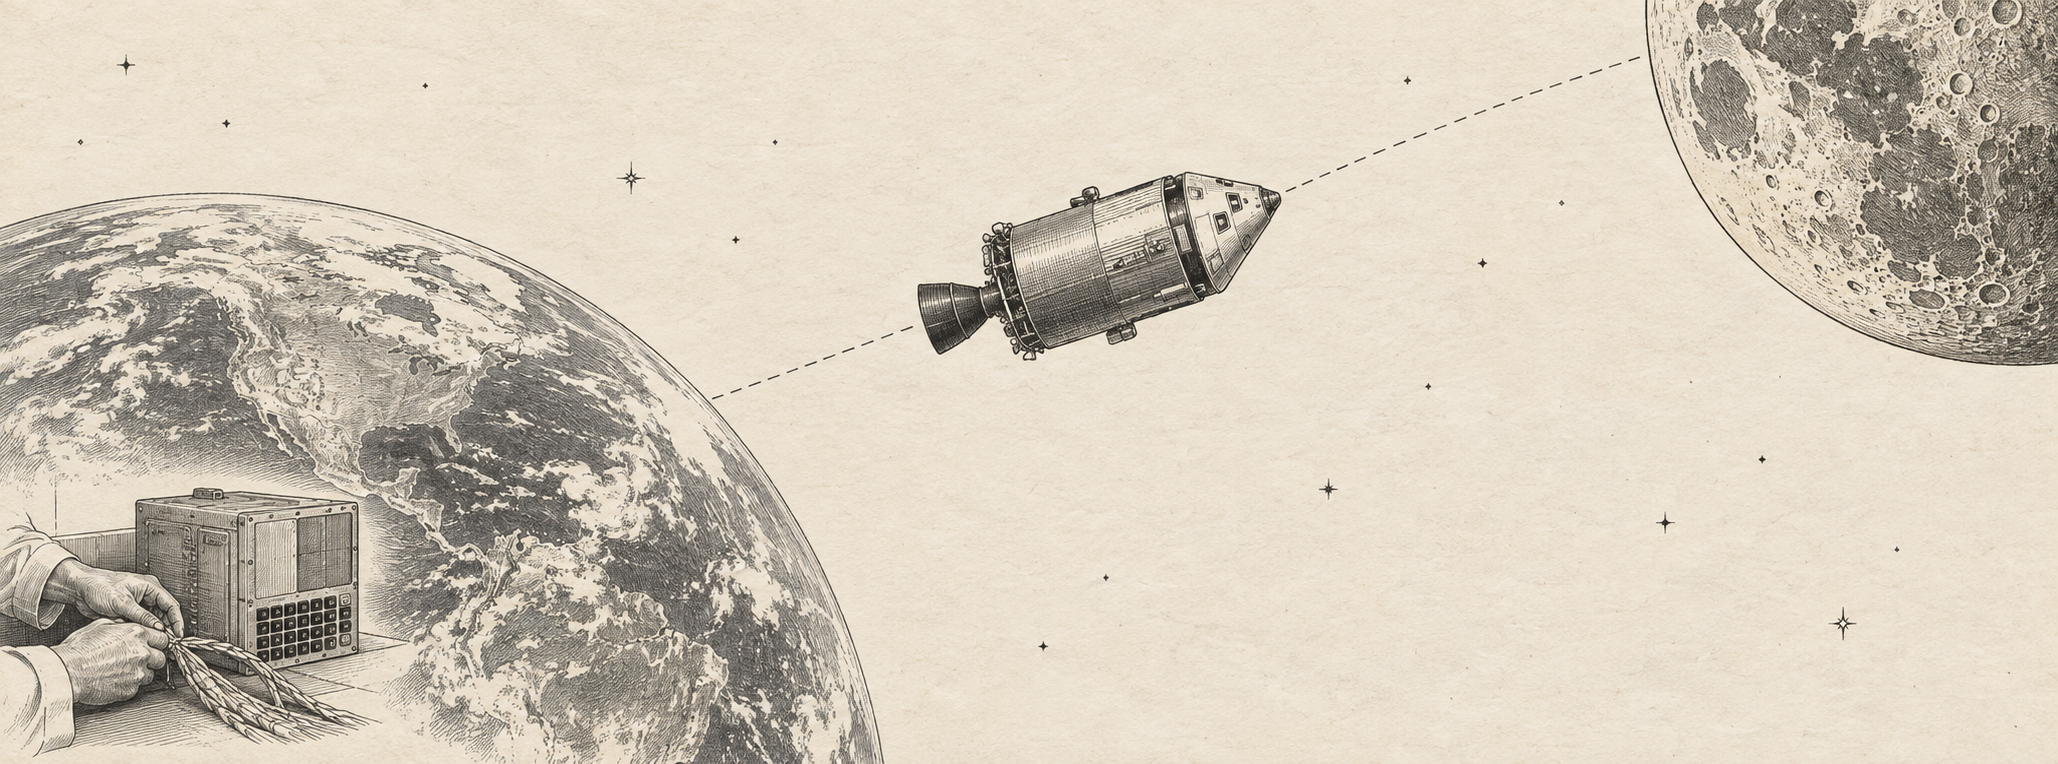
\includegraphics[width=.95\linewidth]{figures/chapter04/apollo_vintage.png}
\captionof{figure}{从地球到月球：航行背后的数学与手艺。复古线描插画为教学创作，飞行轨迹、天体大小与距离均为示意。}
\label{fig:four-apollo-voyage}
\end{minipage}

\par\addvspace{8pt}
\noindent\begin{minipage}{\linewidth}
\noindent{\large\bfseries 一、旋转：坐标轴不动，箭头真的转过去了。}\par
\vspace{5pt}
\centering
\begin{tikzpicture}[font=\small,x=1cm,y=1cm]
 \foreach \offset/\name in {0/旋转前,7.3/旋转后} {
  \begin{scope}[shift={(\offset,0)},x={(-.83cm,-.4cm)},y={(.88cm,-.36cm)},z={(0cm,.90cm)}]
   \fill[FourLight!12] (0,0,0)--(2.6,0,0)--(2.6,2.6,0)--(0,2.6,0)--cycle;
   \draw[fouraxis] (0,0,0)--(3.1,0,0) node[below left] {$x$};
   \draw[fouraxis] (0,0,0)--(0,3.1,0) node[below right] {$y$};
   \draw[fouraxis] (0,0,0)--(0,0,3.4) node[above] {$z$};
   \node[below] at (0,0,0) {$O$};
   \node[font=\small\bfseries] at (0,0,4.15) {\name};
  \end{scope}
 }
 \begin{scope}[x={(-.83cm,-.4cm)},y={(.88cm,-.36cm)},z={(0cm,.90cm)}]
  \draw[fourguide] (2,0,0)--(2,0,2)--(0,0,2);
  \draw[fourvector] (0,0,0)--(2,0,2) node[above left] {$\boldsymbol v$};
  \fill[FourInk] (2,0,2) circle (1.7pt);
 \end{scope}
 \draw[-{Stealth[length=2.3mm]},FourWarm,line width=1pt] (3.05,1.25)--(4.65,1.25);
 \node[align=center,text=FourWarm,font=\footnotesize] at (3.85,2.0) {绕 $z$ 轴\\旋转 $90^\circ$};
 \node[FourWarm] at (3.85,.8) {$A$};
 \begin{scope}[shift={(7.3,0)},x={(-.83cm,-.4cm)},y={(.88cm,-.36cm)},z={(0cm,.90cm)}]
  \draw[FourLight,densely dashed,line width=1pt,-{Stealth[length=2mm]}] (0,0,0)--(2,0,2);
  \node[font=\footnotesize,text=FourLight,below left] at (2,0,2) {原方向};
  \draw[fourguide] (0,2,0)--(0,2,2)--(0,0,2);
  \draw[fourvector] (0,0,0)--(0,2,2) node[above right] {$\boldsymbol v'=A\boldsymbol v$};
  \fill[FourInk] (0,2,2) circle (1.7pt);
  \draw[FourWarm,-{Stealth[length=2mm]},line width=.85pt]
   plot[domain=0:90,samples=25] ({1.15*cos(\x)},{1.15*sin(\x)},.07);
  \node[font=\footnotesize,text=FourWarm,below] at (.86,.86,0) {$90^\circ$};
 \end{scope}
 \node at (0,-2.0) {$\boldsymbol v=(2,0,2)^{\mathrm T}$};
 \node at (7.3,-2.0) {$\boldsymbol v'=(0,2,2)^{\mathrm T}$};
\end{tikzpicture}
\captionof{figure}{固定同一组 $\mathbb R^3$ 坐标轴，向量绕 $z$ 轴旋转。浅色虚线只保留原方向作比较；实线箭头的终点发生了改变。}
\label{fig:four-active-rotation}
\par\vspace{5pt}
\noindent\begin{minipage}[c]{.36\linewidth}
\centering\linespread{1}\fontsize{10.5pt}{14pt}\selectfont
\(\displaystyle
 A=\begin{pmatrix}0&-1&0\\1&0&0\\0&0&1\end{pmatrix},\qquad
 \boldsymbol v'=A\boldsymbol v.
\)
\end{minipage}\hfill
\begin{minipage}[c]{.61\linewidth}
\linespread{1}\fontsize{10pt}{15pt}\selectfont\color{FourInk!85}
\textbf{读图说明}\quad 这里用方向向量代表飞船朝向的一部分。旋转中心取作原点，观察用的坐标轴固定；随船转动的本体系不能同时说成“固定不动”。向量的长度保持不变，$z$ 分量也保持不变。
\end{minipage}
\end{minipage}

\par\addvspace{12pt}\Needspace{11\baselineskip}
\noindent{\large\bfseries 二、换基：箭头没动，只换一组“尺子”。}\par
\vspace{7pt}
下面两幅图画的是同一支向量 $\boldsymbol r$。请先看起点 $O$ 和终点 $R$：它们在两个小图中的位置完全相同。右图只把坐标轴转过 $45^\circ$，因此沿新轴量出的两个分量变了。

\vspace{8pt}
\noindent\begin{minipage}{\linewidth}
\centering
\begin{tikzpicture}[x=1.05cm,y=1.05cm,font=\small]
 \begin{scope}
  \draw[FourLight!40,step=1] (-.45,-.8) grid (3.55,3.0);
  \draw[fouraxis] (-.5,0)--(3.8,0) node[right] {$\boldsymbol e_1$};
  \draw[fouraxis] (0,-1.0)--(0,3.1) node[above] {$\boldsymbol e_2$};
  \draw[fourguide] (0,0)--(3,0)--(3,1);
  \draw[fourvector] (0,0)--(3,1);
  \fill[FourInk] (3,1) circle(1.8pt);
  \node[above right] at (3,1) {$R$};
  \node[below left] at (0,0) {$O$};
  \node[above,fill=white,inner sep=1pt] at (1.45,.52) {$\boldsymbol r$};
  \node[below,text=FourWarm] at (1.5,0) {$3$};
  \node[right,text=FourWarm] at (3,.48) {$1$};
  \node[font=\small\bfseries] at (1.55,3.85) {用原来的基 $E$ 测量};
  \node at (1.55,-1.65) {$[\boldsymbol r]_E=\begin{pmatrix}3\\1\end{pmatrix}$};
 \end{scope}
 \begin{scope}[shift={(7.3,0)}]
  \begin{scope}[overlay]
   \clip (-1.85,-1.0) rectangle (3.6,3.2);
   \begin{scope}[rotate=45]
    \draw[FourLight!40,step=1] (-3,-4) grid (5,4);
   \end{scope}
  \end{scope}
  \draw[fouraxis] (-.6,-.6)--(2.55,2.55) node[above right] {$\boldsymbol m_1$};
  \draw[fouraxis] (.55,-.55)--(-1.65,1.65) node[above left] {$\boldsymbol m_2$};
  \draw[fourguide] (0,0)--(2,2)--(3,1);
  \draw[FourWarm,-{Stealth[length=1.8mm]},line width=.7pt] (2.05,1.95)--(2.8,1.2);
  \draw[fourvector] (0,0)--(3,1);
  \fill[FourInk] (3,1) circle(1.8pt);
  \node[above right] at (3,1) {$R$};
  \node[below left] at (0,0) {$O$};
  \node[above,fill=white,inner sep=1pt] at (1.5,.55) {$\boldsymbol r$};
  \node[above left,text=FourWarm,fill=white,inner sep=1pt] at (1.05,1.05) {$2\sqrt2$};
  \node[above right,text=FourWarm,fill=white,inner sep=1pt] at (2.5,1.55) {$-\sqrt2$};
  \node[font=\small\bfseries] at (1.55,3.85) {用转过的基 $M$ 测量};
  \node at (1.55,-1.65) {$[\boldsymbol r]_M=\begin{pmatrix}2\sqrt2\\-\sqrt2\end{pmatrix}$};
 \end{scope}
\end{tikzpicture}
\par\vspace{-18pt}
\captionof{figure}{同一向量，两组坐标。两幅图中的实线箭头完全相同；虚线表示沿各自坐标轴的分量分解。右图沿 $\boldsymbol m_2$ 的反方向走，所以第二个坐标为负。}
\label{fig:four-passive-basis}
\end{minipage}

在左图，沿 $\boldsymbol e_1$ 走3个单位，再沿 $\boldsymbol e_2$ 走1个单位，就到达 $R$。在右图，先沿 $\boldsymbol m_1$ 走 $2\sqrt2$ 个单位，再沿 $\boldsymbol m_2$ 的反方向走 $\sqrt2$ 个单位，仍到达同一个 $R$。\textbf{换的是分解方式，箭头并没有跟着坐标轴转动。}

把新基向量在旧基下的坐标按列排在一起，就得到矩阵 $P$：
\[
 P=\frac1{\sqrt2}\begin{pmatrix}1&-1\\1&1\end{pmatrix},\qquad
 [\boldsymbol r]_E=P[\boldsymbol r]_M,\qquad
 \boxed{[\boldsymbol r]_M=P^{-1}[\boldsymbol r]_E}.
\]
同样的方法也适用于三维空间：把两组平面坐标轴换成两组三维坐标轴，$P$ 就相应成为一个三阶矩阵。

\FourNote{从换基到真实参考系}{图中的两组基共用原点。地心与月心则是两个不同的原点；若把飞船的地心位置改写为月心位置，还须先减去月心的地心位置 $\boldsymbol c_E$，再换基，即 $\boldsymbol r_M=P^{-1}(\boldsymbol r_E-\boldsymbol c_E)$。因此，“同一自由向量的分量换算”与“同一点相对于不同原点的位置坐标换算”要分清。}

\par\vspace{5pt}\noindent\begin{minipage}{\linewidth}
\centering\bfseries\color{FourWarm}
线性变换：基不动，向量动。\qquad 基变换：向量不动，基动。\par
\vspace{5pt}两类运算，同一套语言——矩阵。
\end{minipage}

\par\Needspace{5\baselineskip}
% FOUR ORIGINAL 12 BEGIN
载人登月这种人类工程巅峰里最底层的操作，本质就是线性代数最核心的两类操作：
% FOUR ORIGINAL 12 END

% FOUR ORIGINAL 13 BEGIN
线性变换描述「向量本身的变化」。 基变换描述「观察视角的变化」。
% FOUR ORIGINAL 13 END

% FOUR ORIGINAL 14 BEGIN
这两件事，看起来相似，实则完全不同。混淆它们，是学习线性代数时最容易犯的错误之一。而区分它们，恰恰是理解矩阵、理解线性代数的关键一步。
% FOUR ORIGINAL 14 END

% FOUR ORIGINAL 15 BEGIN
更值得深思的是：阿波罗11号的导航计算机，从来没有“看见”过月球。它只看见矩阵。它只知道，当前的状态向量，经过某个矩阵作用后，变成了新的状态向量。它只知道，同一个向量，在不同的基下，对应着不同的坐标。但它就是靠这些矩阵运算，把人类送上了月球。
% FOUR ORIGINAL 15 END

% FOUR ORIGINAL 16 BEGIN
这引出了一个更根本的问题：我们究竟是在变换向量，还是在变换我们描述向量的方式？
% FOUR ORIGINAL 16 END

% FOUR ORIGINAL 17 BEGIN
在阿波罗11号之前，这个问题是哲学家的。在阿波罗11号之后，它成了工程师每天都要面对的问题。
% FOUR ORIGINAL 17 END

% FOUR ORIGINAL 18 BEGIN
本章我们就从几何直观出发，先讲线性变换的定义、矩阵表示与运算对应，再讲基变换的原理与相似矩阵。我们会看到，同一个线性变换，在不同基下对应着不同的矩阵；而这些矩阵之间，又由相似变换联系起来。它们描述的是同一个变换，只是穿了不同的“坐标系外衣”。
% FOUR ORIGINAL 18 END

% FOUR ORIGINAL 19 BEGIN
完成这一章，你对矩阵的理解将从“解方程的工具”，升级为“描述世界的框架”。
% FOUR ORIGINAL 19 END

\FourNote{矩阵背后的人}{%
当我们说“矩阵把人类送上月球”，也应看见矩阵背后的人：设计轨道、编写程序、编织存储器、校核数据，以及在关键时刻作出判断的人。一个正负号、一个单位、一组基的约定，都需要被清楚地表达并反复核对。数学的严谨，在这里成为人与人之间能够协作、能够信任的一种语言。}
\par\clearpage
\endgroup

\setcounter{figure}{0}
% APOLLO RESTORATION END

\FHead{本章路线}

屏幕上的图形转过一个角度，或被拉长、压扁，我们看到的是形状，计算机处理的却是顶点的坐标。第三章已经说明：知道标准基向量的像，就能写出线性映射的矩阵；矩阵的乘法，则把连续发生的作用接起来。本章从这些可见的变化出发，追问两个更深的问题：\textbf{哪些输入的差别会在变换中消失？哪些输出是这项变换能够产生的？}

这两个问题将分别引出零空间与值域。它们把第二章的消元计算接到第五章的解的结构：求解 $A\boldsymbol x=\boldsymbol b$，既要问目标 $\boldsymbol b$ 能否到达，也要问到达它的输入是否唯一。第4.1至4.3节是本章主线；第4.4至4.6节为选读，分别讨论换基与相似矩阵、坐标变换的工程语言（以钱学森弹道为例）、秩与零度的严格证明；第4.7节以图像压缩作为选读应用案例。

本章始终在实数空间中讨论。矩阵作用于列向量，$A_{j,k}$ 的第一个下标表示行，第二个下标表示列；$E_n$ 表示 $n$ 阶单位矩阵，尺寸明确时简记为 $E$。

\section{线性变换的几何直观与零空间}
\label{sec:four-geometry-null}
\subsection{计算机图形学中的线性变换}
\label{sec:four-graphics}

\FHead{把图形看成一组顶点}
在计算机图形学中，绕原点旋转、按坐标方向缩放，以及剪切等基本形变，都可以逐个顶点实施矩阵乘法。例如，一张平面图形有四个顶点，就把四个位置向量并排放进矩阵 $X$，用同一个矩阵 $A$ 左乘：$AX$ 的四列便是变换后的顶点。这种统一处理之所以可行，依靠的是线性映射保持线性组合的性质。平移需要稍后的齐次坐标；任意非线性形变与整个渲染过程，则不能一概归结为同一个线性映射。

先取单位正方形，按绕边界的顺序记录顶点：
\[
 X=\FMat{rrrr}{0&1&1&0\\0&0&1&1}.
\]
顶点之间的边也会随之移动。因为线段上的点可写成 $(1-t)\boldsymbol u+t\boldsymbol v$，其中 $0\leq t\leq1$，由线性性质可得
\[
 T\bigl((1-t)\boldsymbol u+t\boldsymbol v\bigr)
 =(1-t)T(\boldsymbol u)+tT(\boldsymbol v).
\]
因此，一条边仍被送成连接两端点像的线段；如果两端点的像重合，整条边就缩成一个点。\textbf{保持线性组合，并不保证不同的点仍然分开。}下面五类变换，正好让我们看见这两种可能。


\FHead{缩放：沿两个方向分别改变尺度}
屏幕上的同一个图标，可能需要单独拉宽或拉高。我们先把横、纵两个方向分开处理，再看它们怎样共同作用于整个图形；这正是对角矩阵最直接的几何含义。

\term{scaling}把横坐标乘 $s_x$，纵坐标乘 $s_y$。标准基向量的像为
\[
 T(\boldsymbol e_1)=(s_x,0)^{\mathrm T},\qquad
 T(\boldsymbol e_2)=(0,s_y)^{\mathrm T}.
\]
利用 $\boldsymbol x=x\boldsymbol e_1+y\boldsymbol e_2$ 与线性组合的保持性，所需规则及矩阵便是
\[
 T(x,y)=(s_xx,s_yy)^{\mathrm T},\qquad
 A=\operatorname{diag}(s_x,s_y)=\FMat{cc}{s_x&0\\0&s_y}.
\]

% FIGURE scale2 BEGIN
\FourFigure{缩放：两个方向分别伸长。}{fig:four-scale2}{%
\begin{tikzpicture}[x=1.2cm,y=1.2cm,every node/.style={font=\small,inner sep=2pt}]
\begin{scope}[shift={(0,0)}]
\node[font=\small\bfseries] at (0.55000,4.15000) {变换前};
\draw[fouraxis] (-1.15000,0.00000)--(2.70000,0.00000);
\node[right] at (2.80000,0.00000) {$x$};
\draw[fouraxis] (0.00000,-0.55000)--(0.00000,3.50000);
\node[above] at (0.00000,3.55000) {$y$};
\node[below left] at (0.00000,0.00000) {$O$};
\draw[FourGray!70,densely dashed,line width=.8pt] (0.00000,0.00000)--(1.00000,0.00000)--(1.00000,1.00000)--(0.00000,1.00000)--cycle;
\draw[fourblue] (0.00000,0.00000)--(1.00000,0.00000);
\node[below,text=FourBlue] at (0.60000,-0.14000) {$\boldsymbol e_1$};
\draw[fourrose] (0.00000,0.00000)--(0.00000,1.00000);
\node[left,text=FourRose] at (-0.12000,0.65000) {$\boldsymbol e_2$};
\node[above right] at (1.00000,1.00000) {$(1,1)$};
\end{scope}
\begin{scope}[shift={(6.1,0)}]
\node[font=\small\bfseries] at (0.55000,4.15000) {变换后};
\draw[fouraxis] (-1.15000,0.00000)--(2.70000,0.00000);
\node[right] at (2.80000,0.00000) {$x$};
\draw[fouraxis] (0.00000,-0.55000)--(0.00000,3.50000);
\node[above] at (0.00000,3.55000) {$y$};
\fill[FourBlue!10] (0.00000,0.00000)--(2.00000,0.00000)--(2.00000,3.00000)--(0.00000,3.00000)--cycle;
\draw[FourGray!70,densely dashed,line width=.8pt] (0.00000,0.00000)--(1.00000,0.00000)--(1.00000,1.00000)--(0.00000,1.00000)--cycle;
\draw[FourBlue,line width=1pt] (0.00000,0.00000)--(2.00000,0.00000)--(2.00000,3.00000)--(0.00000,3.00000)--cycle;
\draw[fourblue] (0.00000,0.00000)--(2.00000,0.00000);
\draw[fourrose] (0.00000,0.00000)--(0.00000,3.00000);
\fill[FourBlue] (0.00000,0.00000) circle(2pt);
\node[below left] at (0.00000,0.00000) {$(0,0)$};
\fill[FourBlue] (2.00000,0.00000) circle(2pt);
\node[below right] at (2.00000,0.00000) {$(2,0)$};
\fill[FourBlue] (2.00000,3.00000) circle(2pt);
\node[above right] at (2.00000,3.00000) {$(2,3)$};
\fill[FourBlue] (0.00000,3.00000) circle(2pt);
\node[above left] at (0.00000,3.00000) {$(0,3)$};
\node[above,text=FourBlue,font=\footnotesize] at (1.00000,0.20000) {$T(\boldsymbol e_1)=2\boldsymbol e_1$};
\node[left,text=FourRose] at (-0.15000,1.70000) {$3\boldsymbol e_2$};
\end{scope}
\draw[fouraxis] (3.15000,0.60000)--(4.25000,0.60000);
\node[above] at (3.70000,0.75000) {$A$};
\end{tikzpicture}
\par\vspace{5pt}{\small $\displaystyle A=\FMat{rr}{2&0\\0&3},\qquad A\FMat{r}{1\\1}=\FMat{r}{2\\3}.$}\par
}{灰色虚线为原图形，实线为变换后的像；两幅子图采用相同坐标比例。}
% FIGURE scale2 END

这里以及下文的 $T(x,y)$，是 $T((x,y)^{\mathrm T})$ 的简写。对 $\boldsymbol u=(u_1,u_2)^{\mathrm T}$、$\boldsymbol v=(v_1,v_2)^{\mathrm T}$，直接代入可得
\[
 \begin{aligned}
 T(\boldsymbol u+\boldsymbol v)
 &=\FMat{c}{s_x(u_1+v_1)\\s_y(u_2+v_2)}\\
 &=\FMat{c}{s_xu_1\\s_yu_2}+\FMat{c}{s_xv_1\\s_yv_2}
 =T(\boldsymbol u)+T(\boldsymbol v).
 \end{aligned}
\]
数乘性质同理由分配律得到，因此这个坐标规则确实定义了线性映射，而不只是看起来像一个几何变形。

取 $s_x=2,s_y=3$，则
\[
 AX=\FMat{rrrr}{0&2&2&0\\0&0&3&3}.
\]
原来横、纵边长都为1的正方形，变成横边长2、纵边长3的矩形。比如 $(1,1)^{\mathrm T}$ 被送到 $(2,3)^{\mathrm T}$，而 $(1,0)^{\mathrm T}+(0,1)^{\mathrm T}$ 的像，恰好也是两条变换后边向量之和。

正的缩放因子表示同向伸缩，负的因子还会翻转相应坐标方向。因子为0时则发生完全压缩。例如 $s_x=2,s_y=0$ 把整个平面压到 $x$ 轴上。\textbf{只有 $s_x\ne0$ 且 $s_y\ne0$ 时，缩放才能用分别除以两个因子的办法恢复原输入。}这个条件稍后会成为判断零空间的关键。

\FHead{旋转：改变方向，保留长度和夹角}
把平面绕原点逆时针转过 $\theta$。从单位圆看，$\boldsymbol e_1$ 的像为 $(\cos\theta,\sin\theta)^{\mathrm T}$，$\boldsymbol e_2$ 的像为 $(-\sin\theta,\cos\theta)^{\mathrm T}$。按第三章“基的像作列”的规则，得到
\[
 A_\theta=\FMat{rr}{\cos\theta&-\sin\theta\\\sin\theta&\cos\theta},\qquad
 T(x,y)=(x\cos\theta-y\sin\theta,\ x\sin\theta+y\cos\theta)^{\mathrm T}.
\]

% FIGURE rotate2 BEGIN
\FourFigure{旋转：绕原点逆时针转过 $60^\circ$。}{fig:four-rotate2}{%
\begin{tikzpicture}[x=1.2cm,y=1.2cm,every node/.style={font=\small,inner sep=2pt}]
\begin{scope}[shift={(0,0)}]
\node[font=\small\bfseries] at (0.55000,2.70000) {变换前};
\draw[fouraxis] (-1.15000,0.00000)--(2.70000,0.00000);
\node[right] at (2.80000,0.00000) {$x$};
\draw[fouraxis] (0.00000,-0.55000)--(0.00000,2.05000);
\node[above] at (0.00000,2.10000) {$y$};
\node[below left] at (0.00000,0.00000) {$O$};
\draw[FourGray!70,densely dashed,line width=.8pt] (0.00000,0.00000)--(1.00000,0.00000)--(1.00000,1.00000)--(0.00000,1.00000)--cycle;
\draw[fourblue] (0.00000,0.00000)--(1.00000,0.00000);
\node[below,text=FourBlue] at (0.60000,-0.14000) {$\boldsymbol e_1$};
\draw[fourrose] (0.00000,0.00000)--(0.00000,1.00000);
\node[left,text=FourRose] at (-0.12000,0.65000) {$\boldsymbol e_2$};
\node[above right] at (1.00000,1.00000) {$(1,1)$};
\end{scope}
\begin{scope}[shift={(6.1,0)}]
\node[font=\small\bfseries] at (0.55000,2.70000) {变换后};
\draw[fouraxis] (-1.15000,0.00000)--(2.70000,0.00000);
\node[right] at (2.80000,0.00000) {$x$};
\draw[fouraxis] (0.00000,-0.55000)--(0.00000,2.05000);
\node[above] at (0.00000,2.10000) {$y$};
\node[below left] at (0.00000,0.00000) {$O$};
\fill[FourBlue!10] (0.00000,0.00000)--(0.50000,0.86603)--(-0.36603,1.36603)--(-0.86603,0.50000)--cycle;
\draw[FourGray!70,densely dashed,line width=.8pt] (0.00000,0.00000)--(1.00000,0.00000)--(1.00000,1.00000)--(0.00000,1.00000)--cycle;
\draw[FourBlue,line width=1pt] (0.00000,0.00000)--(0.50000,0.86603)--(-0.36603,1.36603)--(-0.86603,0.50000)--cycle;
\draw[fourblue] (0.00000,0.00000)--(0.50000,0.86603);
\draw[fourrose] (0.00000,0.00000)--(-0.86603,0.50000);
\draw[FourRose,densely dashed,-{Stealth[length=1.6mm]}] (.65,0) arc[start angle=0,end angle=60,radius=.65];
\node[text=FourRose] at (0.90000,0.40000) {$60^\circ$};
\node[above right,text=FourBlue] at (0.50000,0.86603) {$T(\boldsymbol e_1)$};
\node[above left,text=FourRose] at (-0.86603,0.50000) {$T(\boldsymbol e_2)$};
\end{scope}
\draw[fouraxis] (3.15000,0.60000)--(4.25000,0.60000);
\node[above] at (3.70000,0.75000) {$A$};
\end{tikzpicture}
\par\vspace{5pt}{\small $\displaystyle A=\frac12\FMat{cc}{1&-\sqrt3\\[3pt]\sqrt3&1},\qquad A\FMat{r}{1\\0}=\frac12\FMat{c}{1\\[3pt]\sqrt3}\approx\FMat{c}{0.5\\0.866}.$}\par
}{灰色虚线为原图形，实线为变换后的像；两幅子图采用相同坐标比例。 虚线弧从正 $x$ 轴转向第一列的像。}
% FIGURE rotate2 END

这不是另背一套坐标口诀：第一列记录横向单位箭头转到哪里，第二列记录纵向单位箭头转到哪里，再用 $x,y$ 组合两列。

把 $c\boldsymbol u$ 代入，两项中的 $c$ 都能提出，因此
\[
 T(c\boldsymbol u)=
 c\FMat{c}{u_1\cos\theta-u_2\sin\theta\\u_1\sin\theta+u_2\cos\theta}
 =cT(\boldsymbol u).
\]
可加性同样来自各坐标表达式的分配律。又由 $\cos^2\theta+\sin^2\theta=1$，展开两个输出分量的平方和，有
\[
 (x\cos\theta-y\sin\theta)^2+(x\sin\theta+y\cos\theta)^2=x^2+y^2.
\]
所以长度不变。将同样计算用于两个向量的差，可知两点间距离也不变；于是由三角形的边长关系，夹角也保持不变。

图\ref{fig:four-rotate2}中取 $\theta=60^\circ$。第一列的像为 $(\tfrac12,\tfrac{\sqrt3}{2})^{\mathrm T}$，小数 $(0.5,0.866)^{\mathrm T}$ 只是近似；图形的边长仍为1。再取 $\theta=90^\circ$，$A_\theta=\FMat{rr}{0&-1\\1&0}$，故
\[
 T(1,0)=(0,1)^{\mathrm T},\qquad T(1,1)=(-1,1)^{\mathrm T}.
\]
正方形整体转动，既没有拉长，也没有压扁。将角度改为 $-\theta$ 就能转回去；任意向量若旋转后为零，原先也只能为零。

\FHead{剪切：高度不变，横向偏移随高度改变}
\term{shear}可以想成推动一叠纸的上部：底边固定，越高处横向移动得越多。令偏移量为原高度的 $k$ 倍，则
\[
 T(x,y)=(x+ky,y)^{\mathrm T},\qquad
 T(\boldsymbol e_1)=\boldsymbol e_1,\quad T(\boldsymbol e_2)=(k,1)^{\mathrm T},
 \qquad A=\FMat{rr}{1&k\\0&1}.
\]

% FIGURE shear2 BEGIN
\FourFigure{剪切：底边不动，上边向右移动。}{fig:four-shear2}{%
\begin{tikzpicture}[x=1.2cm,y=1.2cm,every node/.style={font=\small,inner sep=2pt}]
\begin{scope}[shift={(0,0)}]
\node[font=\small\bfseries] at (0.55000,2.70000) {变换前};
\draw[fouraxis] (-1.15000,0.00000)--(2.70000,0.00000);
\node[right] at (2.80000,0.00000) {$x$};
\draw[fouraxis] (0.00000,-0.55000)--(0.00000,2.05000);
\node[above] at (0.00000,2.10000) {$y$};
\node[below left] at (0.00000,0.00000) {$O$};
\draw[FourGray!70,densely dashed,line width=.8pt] (0.00000,0.00000)--(1.00000,0.00000)--(1.00000,1.00000)--(0.00000,1.00000)--cycle;
\draw[fourblue] (0.00000,0.00000)--(1.00000,0.00000);
\node[below,text=FourBlue] at (0.60000,-0.14000) {$\boldsymbol e_1$};
\draw[fourrose] (0.00000,0.00000)--(0.00000,1.00000);
\node[left,text=FourRose] at (-0.12000,0.65000) {$\boldsymbol e_2$};
\node[above right] at (1.00000,1.00000) {$(1,1)$};
\end{scope}
\begin{scope}[shift={(6.1,0)}]
\node[font=\small\bfseries] at (0.55000,2.70000) {变换后};
\draw[fouraxis] (-1.15000,0.00000)--(2.70000,0.00000);
\node[right] at (2.80000,0.00000) {$x$};
\draw[fouraxis] (0.00000,-0.55000)--(0.00000,2.05000);
\node[above] at (0.00000,2.10000) {$y$};
\node[below left] at (0.00000,0.00000) {$O$};
\fill[FourBlue!10] (0.00000,0.00000)--(1.00000,0.00000)--(2.00000,1.00000)--(1.00000,1.00000)--cycle;
\draw[FourGray!70,densely dashed,line width=.8pt] (0.00000,0.00000)--(1.00000,0.00000)--(1.00000,1.00000)--(0.00000,1.00000)--cycle;
\draw[FourBlue,line width=1pt] (0.00000,0.00000)--(1.00000,0.00000)--(2.00000,1.00000)--(1.00000,1.00000)--cycle;
\draw[fourblue] (0.00000,0.00000)--(1.00000,0.00000);
\draw[fourrose] (0.00000,0.00000)--(1.00000,1.00000);
\draw[fourrose] (0.45000,1.35000)--(1.45000,1.35000);
\node[above] at (1.00000,1.55000) {上边右移1};
\node[below] at (0.50000,-0.40000) {底边不动};
\node[above right] at (2.00000,1.00000) {$(2,1)$};
\node[above left] at (1.00000,1.00000) {$(1,1)$};
\end{scope}
\draw[fouraxis] (3.15000,0.60000)--(4.25000,0.60000);
\node[above] at (3.70000,0.75000) {$A$};
\end{tikzpicture}
\par\vspace{5pt}{\small $\displaystyle A=\FMat{rr}{1&1\\0&1},\qquad A\FMat{r}{0\\1}=\FMat{r}{1\\1}.$}\par
}{灰色虚线为原图形，实线为变换后的像；两幅子图采用相同坐标比例。}
% FIGURE shear2 END

第二个分量没有改变；第一个分量同时接收原来的横坐标和由高度带来的偏移。对任意 $\boldsymbol u,\boldsymbol v$，
\[
 T(\boldsymbol u+\boldsymbol v)
 =\FMat{c}{u_1+v_1+k(u_2+v_2)\\u_2+v_2}
 =T(\boldsymbol u)+T(\boldsymbol v),
\]
且 $T(c\boldsymbol u)=cT(\boldsymbol u)$，所以剪切仍然线性。

取 $k=1$，单位正方形的四个顶点依次变成 $(0,0)$、$(1,0)$、$(2,1)$、$(1,1)$，围成平行四边形。例如 $T(0,1)=(1,1)^{\mathrm T}$，但底边上的每一点 $(x,0)$ 保持不动。图形虽然变斜，信息却没有丢失：从输出 $(p,q)$ 先读出 $y=q$，再算 $x=p-kq$，就能唯一找回输入。相应的逆矩阵为 $\FMat{rr}{1&-k\\0&1}$，对任意实数 $k$ 都存在。

\FHead{反射：把一侧翻到另一侧}
\term{reflection}保持镜面上的点不动，将垂直于镜面的方向反向。关于 $x$ 轴、关于 $y$ 轴、关于直线 $y=x$ 的反射，分别为
\[
 \begin{array}{c|c|c}
 \text{反射轴}&T(x,y)&A\\ \hline\noalign{\vskip4pt}
 x\text{轴}&(x,-y)^{\mathrm T}&\FMat{rr}{1&0\\0&-1}\\\noalign{\vskip6pt}
 y\text{轴}&(-x,y)^{\mathrm T}&\FMat{rr}{-1&0\\0&1}\\\noalign{\vskip6pt}
 y=x&(y,x)^{\mathrm T}&\FMat{rr}{0&1\\1&0}
 \end{array}
\]

% FIGURE reflect2 BEGIN
\FourFigure{反射：正方形关于 $x$ 轴翻到下方。}{fig:four-reflect2}{%
\begin{tikzpicture}[x=1.2cm,y=1.2cm,every node/.style={font=\small,inner sep=2pt}]
\begin{scope}[shift={(0,0)}]
\node[font=\small\bfseries] at (0.55000,2.45000) {变换前};
\draw[fouraxis] (-1.15000,0.00000)--(2.70000,0.00000);
\node[right] at (2.80000,0.00000) {$x$};
\draw[fouraxis] (0.00000,-1.50000)--(0.00000,1.80000);
\node[above] at (0.00000,1.85000) {$y$};
\node[below left] at (0.00000,0.00000) {$O$};
\draw[FourGray!70,densely dashed,line width=.8pt] (0.00000,0.00000)--(1.00000,0.00000)--(1.00000,1.00000)--(0.00000,1.00000)--cycle;
\draw[fourblue] (0.00000,0.00000)--(1.00000,0.00000);
\node[below,text=FourBlue] at (0.60000,-0.14000) {$\boldsymbol e_1$};
\draw[fourrose] (0.00000,0.00000)--(0.00000,1.00000);
\node[left,text=FourRose] at (-0.12000,0.65000) {$\boldsymbol e_2$};
\node[above right] at (1.00000,1.00000) {$(1,1)$};
\end{scope}
\begin{scope}[shift={(6.1,0)}]
\node[font=\small\bfseries] at (0.55000,2.45000) {变换后};
\draw[fouraxis] (-1.15000,0.00000)--(2.70000,0.00000);
\node[right] at (2.80000,0.00000) {$x$};
\draw[fouraxis] (0.00000,-1.50000)--(0.00000,1.80000);
\node[above] at (0.00000,1.85000) {$y$};
\node[below left] at (0.00000,0.00000) {$O$};
\fill[FourBlue!10] (0.00000,0.00000)--(1.00000,0.00000)--(1.00000,-1.00000)--(0.00000,-1.00000)--cycle;
\draw[FourGray!70,densely dashed,line width=.8pt] (0.00000,0.00000)--(1.00000,0.00000)--(1.00000,1.00000)--(0.00000,1.00000)--cycle;
\draw[FourBlue,line width=1pt] (0.00000,0.00000)--(1.00000,0.00000)--(1.00000,-1.00000)--(0.00000,-1.00000)--cycle;
\draw[fourblue] (0.00000,0.00000)--(1.00000,0.00000);
\draw[fourrose] (0.00000,0.00000)--(0.00000,-1.00000);
\draw[FourGreen,densely dashed,line width=1pt] (-1.15000,0.00000)--(2.40000,0.00000);
\node[above,text=FourGreen] at (1.75000,0.17000) {镜像轴：$x$轴};
\draw[fourguide] (1.00000,1.00000)--(1.00000,-1.00000);
\node[right,text=FourRose] at (0.12000,-0.65000) {$-\boldsymbol e_2$};
\node[below right] at (1.00000,-1.00000) {$(1,-1)$};
\end{scope}
\draw[fouraxis] (3.15000,0.60000)--(4.25000,0.60000);
\node[above] at (3.70000,0.75000) {$A$};
\end{tikzpicture}
\par\vspace{5pt}{\small $\displaystyle A=\FMat{rr}{1&0\\0&-1},\qquad A\FMat{r}{2\\3}=\FMat{r}{2\\-3}.$}\par
}{灰色虚线为原图形，实线为变换后的像；两幅子图采用相同坐标比例。 绿色虚线标出保持不动的镜像轴。}
% FIGURE reflect2 END

这些矩阵仍由两个标准基向量的像按列排出。以关于 $x$ 轴反射为例，
\[
 T(\boldsymbol u+\boldsymbol v)
 =(u_1+v_1,-u_2-v_2)^{\mathrm T}
 =T(\boldsymbol u)+T(\boldsymbol v),
\]
数乘性质也成立。其余两种反射分别只改变一个分量的符号或交换两个分量，验证方法相同。

数值上，$(2,3)^{\mathrm T}$ 关于 $x$ 轴的像是 $(2,-3)^{\mathrm T}$；再反射一次便回到 $(2,3)^{\mathrm T}$。一般地，这三种反射均满足
\[
 T(T(\boldsymbol u))=\boldsymbol u,\qquad A^2=E_2,
\]
所以逆变换就是自身。要分清两件事：可加性、齐次性说明它是线性映射；反射两次恢复原状说明它可逆，后一个性质不能单独替代线性检验。

\FHead{正交投影：留下一个方向，舍去另一个方向}
向 $x$ 轴作\term{orthogonal-projection}，相当于从每一点沿竖直方向落到 $x$ 轴。它保留横坐标、舍去纵坐标：
\[
 T(x,y)=(x,0)^{\mathrm T},\qquad
 T(\boldsymbol e_1)=\boldsymbol e_1,\quad T(\boldsymbol e_2)=\boldsymbol0,
 \qquad A=\FMat{rr}{1&0\\0&0}.
\]

% FIGURE project2 BEGIN
\FourFigure{投影：正方形被压成 $x$ 轴上的线段。}{fig:four-project2}{%
\begin{tikzpicture}[x=1.2cm,y=1.2cm,every node/.style={font=\small,inner sep=2pt}]
\begin{scope}[shift={(0,0)}]
\node[font=\small\bfseries] at (0.55000,2.70000) {变换前};
\draw[fouraxis] (-1.15000,0.00000)--(2.70000,0.00000);
\node[right] at (2.80000,0.00000) {$x$};
\draw[fouraxis] (0.00000,-0.55000)--(0.00000,2.05000);
\node[above] at (0.00000,2.10000) {$y$};
\node[below left] at (0.00000,0.00000) {$O$};
\draw[FourGray!70,densely dashed,line width=.8pt] (0.00000,0.00000)--(1.00000,0.00000)--(1.00000,1.00000)--(0.00000,1.00000)--cycle;
\draw[fourblue] (0.00000,0.00000)--(1.00000,0.00000);
\node[below,text=FourBlue] at (0.60000,-0.14000) {$\boldsymbol e_1$};
\draw[fourrose] (0.00000,0.00000)--(0.00000,1.00000);
\node[left,text=FourRose] at (-0.12000,0.65000) {$\boldsymbol e_2$};
\node[above right] at (1.00000,1.00000) {$(1,1)$};
\end{scope}
\begin{scope}[shift={(6.1,0)}]
\node[font=\small\bfseries] at (0.55000,2.70000) {变换后};
\draw[fouraxis] (-1.15000,0.00000)--(2.70000,0.00000);
\node[right] at (2.80000,0.00000) {$x$};
\draw[fouraxis] (0.00000,-0.55000)--(0.00000,2.05000);
\node[above] at (0.00000,2.10000) {$y$};
\node[below left] at (0.00000,0.00000) {$O$};
\draw[FourGray!70,densely dashed,line width=.8pt] (0.00000,0.00000)--(1.00000,0.00000)--(1.00000,1.00000)--(0.00000,1.00000)--cycle;
\draw[FourBlue,line width=2.6pt] (0.00000,0.00000)--(1.00000,0.00000);
\draw[fourguide,-{Stealth[length=1.6mm]}] (0.00000,1.00000)--(0.00000,0.07000);
\draw[fourguide,-{Stealth[length=1.6mm]}] (0.50000,1.00000)--(0.50000,0.07000);
\draw[fourguide,-{Stealth[length=1.6mm]}] (1.00000,1.00000)--(1.00000,0.07000);
\fill[FourRose] (0.00000,0.00000) circle(2pt);
\node[text=FourRose] at (1.10000,1.45000) {$T(\boldsymbol e_2)=\boldsymbol0$};
\node[text=FourBlue] at (1.40000,-0.40000) {$T(\boldsymbol e_1)=\boldsymbol e_1$};
\end{scope}
\draw[fouraxis] (3.15000,0.60000)--(4.25000,0.60000);
\node[above] at (3.70000,0.75000) {$A$};
\end{tikzpicture}
\par\vspace{5pt}{\small $\displaystyle A=\FMat{rr}{1&0\\0&0},\qquad A\FMat{r}{3\\4}=\FMat{r}{3\\0}.$}\par
}{灰色虚线为原图形，实线为变换后的像；两幅子图采用相同坐标比例。 竖直虚线箭头表示高度被舍去，$y$ 轴上的输入都被送到原点。}
% FIGURE project2 END

相应地，向 $y$ 轴的投影矩阵是 $\FMat{rr}{0&0\\0&1}$。直接检查，例如
\[
 T(\boldsymbol u+\boldsymbol v)=(u_1+v_1,0)^{\mathrm T}
 =T(\boldsymbol u)+T(\boldsymbol v),\qquad
 T(c\boldsymbol u)=cT(\boldsymbol u),
\]
可知投影也完全符合线性性质。线性不等于可逆，投影正是最重要的提醒。

如果目标是与 $x$ 轴夹角为 $\alpha$ 的过原点直线，取沿直线的单位方向 $\boldsymbol d=(\cos\alpha,\sin\alpha)^{\mathrm T}$。投影点形如 $t\boldsymbol d$；由垂足条件，原向量减去投影后的剩余部分与直线垂直，即
\[
 (x-t\cos\alpha)\cos\alpha+(y-t\sin\alpha)\sin\alpha=0.
\]
利用单位方向的长度为1，解得 $t=x\cos\alpha+y\sin\alpha$，所以
\[
 T(x,y)=(x\cos\alpha+y\sin\alpha)\FMat{c}{\cos\alpha\\\sin\alpha},\qquad
 A=\FMat{cc}{\cos^2\alpha&\cos\alpha\sin\alpha\\
 \cos\alpha\sin\alpha&\sin^2\alpha}.
\]
这里仅用到了高中平面向量的垂直条件，第7章会系统讨论这种正交关系。两分量都是 $x,y$ 的固定线性组合，故仍保持加法与数乘。

现在回到 $x$ 轴投影。$(3,4)^{\mathrm T}$ 被送到 $(3,0)^{\mathrm T}$，$(3,-2)^{\mathrm T}$ 也被送到同一个点。只看到输出 $(3,0)^{\mathrm T}$，就无法知道原来的高度。这是\textbf{信息丢失}：整条竖直直线上的输入，在输出中只留下一个点。

把它写成方程组，更能看清缺少了什么：
\[
 \FMat{rr}{1&0\\0&0}\FMat{c}{x_1\\x_2}
 =\FMat{c}{b_1\\b_2}
 \quad\Longleftrightarrow\quad x_1=b_1,\quad 0=b_2.
\]
若 $b_2\ne0$，方程组无解；若 $b_2=0$，$x_2$ 任取，便有无穷多解。几何里的“压缩”，在方程组中留下了自由变量；几何里的“只能落在轴上”，在方程组中留下了对右端项的限制。

\subsubsection*{三维图形学中的线性变换}
\label{sec:four-graphics3}
平面图形只记录横、纵坐标；三维模型还需要记录高度。给一个物体的所有顶点同时左乘同一个 $3\times3$ 矩阵，就能统一改变它的姿态和尺度。为了看清空间感，下面保留三根坐标轴，以浅色面区分立方体的朝向；所有图都先在 $\mathbb R^3$ 中计算顶点，再投影到纸面。

\FHead{绕坐标轴旋转：一个方向不动，另两个方向配合转动}
三维旋转先要回答“绕哪根轴”。绕 $x$ 轴时，$x$ 坐标不变，$y,z$ 两个分量按二维旋转规则变化；绕其余两轴时同理。固定右手坐标系，正转角按右手法则规定，三个矩阵分别为

% FIGURE rotations3 BEGIN
\FourFigure{三维旋转：轴上的点不动，其余点绕轴转动。}{fig:four-rotations3}{%
\begin{tikzpicture}[every node/.style={font=\small,inner sep=2pt}]
\fill[FourBlue!8] (0.73482,-0.03967)--(1.35000,-0.57000)--(1.96518,1.02099)--(1.35000,1.55132)--cycle;
\fill[FourBlue!12] (1.35000,-0.57000)--(0.73482,-0.03967)--(-0.61518,0.53033)--(0.00000,0.00000)--cycle;
\fill[FourBlue!16] (-0.61518,0.53033)--(0.73482,-0.03967)--(1.35000,1.55132)--(0.00000,2.12132)--cycle;
\draw[FourBlue,line width=1pt] (0.00000,0.00000)--(-0.61518,0.53033);
\draw[FourBlue,line width=1pt,densely dashed,opacity=.6] (0.00000,0.00000)--(0.61518,1.59099);
\draw[FourBlue,line width=1pt] (0.00000,0.00000)--(1.35000,-0.57000);
\draw[FourBlue,line width=1pt] (-0.61518,0.53033)--(0.00000,2.12132);
\draw[FourBlue,line width=1pt] (-0.61518,0.53033)--(0.73482,-0.03967);
\draw[FourBlue,line width=1pt,densely dashed,opacity=.6] (0.61518,1.59099)--(0.00000,2.12132);
\draw[FourBlue,line width=1pt,densely dashed,opacity=.6] (0.61518,1.59099)--(1.96518,1.02099);
\draw[FourBlue,line width=1pt] (0.00000,2.12132)--(1.35000,1.55132);
\draw[FourBlue,line width=1pt] (1.35000,-0.57000)--(0.73482,-0.03967);
\draw[FourBlue,line width=1pt] (1.35000,-0.57000)--(1.96518,1.02099);
\draw[FourBlue,line width=1pt] (0.73482,-0.03967)--(1.35000,1.55132);
\draw[FourBlue,line width=1pt] (1.96518,1.02099)--(1.35000,1.55132);
\draw[FourGray!65,densely dashed,line width=.7pt] (0.00000,0.00000)--(0.00000,1.50000);
\draw[FourGray!65,densely dashed,line width=.7pt] (0.00000,0.00000)--(0.87000,0.75000);
\draw[FourGray!65,densely dashed,line width=.7pt] (0.00000,0.00000)--(1.35000,-0.57000);
\draw[FourGray!65,densely dashed,line width=.7pt] (0.00000,1.50000)--(0.87000,2.25000);
\draw[FourGray!65,densely dashed,line width=.7pt] (0.00000,1.50000)--(1.35000,0.93000);
\draw[FourGray!65,densely dashed,line width=.7pt] (0.87000,0.75000)--(0.87000,2.25000);
\draw[FourGray!65,densely dashed,line width=.7pt] (0.87000,0.75000)--(2.22000,0.18000);
\draw[FourGray!65,densely dashed,line width=.7pt] (0.87000,2.25000)--(2.22000,1.68000);
\draw[FourGray!65,densely dashed,line width=.7pt] (1.35000,-0.57000)--(1.35000,0.93000);
\draw[FourGray!65,densely dashed,line width=.7pt] (1.35000,-0.57000)--(2.22000,0.18000);
\draw[FourGray!65,densely dashed,line width=.7pt] (1.35000,0.93000)--(2.22000,1.68000);
\draw[FourGray!65,densely dashed,line width=.7pt] (2.22000,0.18000)--(2.22000,1.68000);
\draw[fouraxis] (-0.47250,0.19950)--(2.36250,-0.99750);
\node[right] at (2.36250,-0.99750) {$x$};
\draw[fouraxis] (-0.30450,-0.26250)--(1.43550,1.23750);
\node[right] at (1.43550,1.23750) {$y$};
\draw[fouraxis] (0.00000,-0.52500)--(0.00000,2.62500);
\node[above] at (0.00000,2.62500) {$z$};
\node[below left] at (0.00000,0.00000) {$O$};
\draw[fourrose] (0.00000,0.00000)--(2.22750,-0.94050);
\draw[FourRose,densely dashed,-{Stealth[length=1.6mm]}] (0.57420,0.49500)--(0.57315,0.55387)--(0.57001,0.61072)--(0.56479,0.66534)--(0.55751,0.71754)--(0.54820,0.76711)--(0.53689,0.81389)--(0.52361,0.85770)--(0.50843,0.89838)--(0.49139,0.93578)--(0.47256,0.96976)--(0.45200,1.00021)--(0.42979,1.02700)--(0.40602,1.05005);
\node[font=\small\bfseries] at (1.00000,3.40000) {绕 $x$ 轴旋转 $45^\circ$};
\node[font=\footnotesize] at (1.00000,-2.20000) {\setlength{\arraycolsep}{2.5pt}$\displaystyle R_x=\FMat{rrr}{1&0&0\\0&\cos\theta&-\sin\theta\\0&\sin\theta&\cos\theta}$};
\fill[FourBlue!8] (5.20000,0.00000)--(6.15459,0.65761)--(7.02459,1.40761)--(6.07000,0.75000)--cycle;
\fill[FourBlue!12] (6.15459,-1.46371)--(7.10919,-0.80610)--(6.15459,0.65761)--(5.20000,0.00000)--cycle;
\fill[FourBlue!16] (7.10919,-0.80610)--(7.97919,-0.05610)--(7.02459,1.40761)--(6.15459,0.65761)--cycle;
\draw[FourBlue,line width=1pt] (5.20000,0.00000)--(6.15459,0.65761);
\draw[FourBlue,line width=1pt] (5.20000,0.00000)--(6.07000,0.75000);
\draw[FourBlue,line width=1pt] (5.20000,0.00000)--(6.15459,-1.46371);
\draw[FourBlue,line width=1pt] (6.15459,0.65761)--(7.02459,1.40761);
\draw[FourBlue,line width=1pt] (6.15459,0.65761)--(7.10919,-0.80610);
\draw[FourBlue,line width=1pt] (6.07000,0.75000)--(7.02459,1.40761);
\draw[FourBlue,line width=1pt,densely dashed,opacity=.6] (6.07000,0.75000)--(7.02459,-0.71371);
\draw[FourBlue,line width=1pt] (7.02459,1.40761)--(7.97919,-0.05610);
\draw[FourBlue,line width=1pt] (6.15459,-1.46371)--(7.10919,-0.80610);
\draw[FourBlue,line width=1pt,densely dashed,opacity=.6] (6.15459,-1.46371)--(7.02459,-0.71371);
\draw[FourBlue,line width=1pt] (7.10919,-0.80610)--(7.97919,-0.05610);
\draw[FourBlue,line width=1pt,densely dashed,opacity=.6] (7.02459,-0.71371)--(7.97919,-0.05610);
\draw[FourGray!65,densely dashed,line width=.7pt] (5.20000,0.00000)--(5.20000,1.50000);
\draw[FourGray!65,densely dashed,line width=.7pt] (5.20000,0.00000)--(6.07000,0.75000);
\draw[FourGray!65,densely dashed,line width=.7pt] (5.20000,0.00000)--(6.55000,-0.57000);
\draw[FourGray!65,densely dashed,line width=.7pt] (5.20000,1.50000)--(6.07000,2.25000);
\draw[FourGray!65,densely dashed,line width=.7pt] (5.20000,1.50000)--(6.55000,0.93000);
\draw[FourGray!65,densely dashed,line width=.7pt] (6.07000,0.75000)--(6.07000,2.25000);
\draw[FourGray!65,densely dashed,line width=.7pt] (6.07000,0.75000)--(7.42000,0.18000);
\draw[FourGray!65,densely dashed,line width=.7pt] (6.07000,2.25000)--(7.42000,1.68000);
\draw[FourGray!65,densely dashed,line width=.7pt] (6.55000,-0.57000)--(6.55000,0.93000);
\draw[FourGray!65,densely dashed,line width=.7pt] (6.55000,-0.57000)--(7.42000,0.18000);
\draw[FourGray!65,densely dashed,line width=.7pt] (6.55000,0.93000)--(7.42000,1.68000);
\draw[FourGray!65,densely dashed,line width=.7pt] (7.42000,0.18000)--(7.42000,1.68000);
\draw[fouraxis] (4.72750,0.19950)--(7.56250,-0.99750);
\node[right] at (7.56250,-0.99750) {$x$};
\draw[fouraxis] (4.89550,-0.26250)--(6.63550,1.23750);
\node[right] at (6.63550,1.23750) {$y$};
\draw[fouraxis] (5.20000,-0.52500)--(5.20000,2.62500);
\node[above] at (5.20000,2.62500) {$z$};
\node[below left] at (5.20000,0.00000) {$O$};
\draw[fourrose] (5.20000,0.00000)--(6.63550,1.23750);
\draw[FourRose,densely dashed,-{Stealth[length=1.6mm]}] (5.20000,0.99000)--(5.25380,0.96548)--(5.30740,0.93744)--(5.36061,0.90597)--(5.41323,0.87120)--(5.46508,0.83325)--(5.51595,0.79226)--(5.56568,0.74838)--(5.61407,0.70177)--(5.66095,0.65260)--(5.70615,0.60105)--(5.74950,0.54730)--(5.79084,0.49156)--(5.83003,0.43402);
\node[font=\small\bfseries] at (6.20000,3.40000) {绕 $y$ 轴旋转 $45^\circ$};
\node[font=\footnotesize] at (6.20000,-2.20000) {\setlength{\arraycolsep}{2.5pt}$\displaystyle R_y=\FMat{rrr}{\cos\theta&0&\sin\theta\\0&1&0\\-\sin\theta&0&\cos\theta}$};
\fill[FourBlue!8] (10.06059,0.93338)--(10.40000,0.00000)--(10.40000,1.50000)--(10.06059,2.43338)--cycle;
\fill[FourBlue!12] (10.40000,0.00000)--(11.96978,0.12728)--(11.96978,1.62728)--(10.40000,1.50000)--cycle;
\fill[FourBlue!16] (10.40000,1.50000)--(11.96978,1.62728)--(11.63037,2.56066)--(10.06059,2.43338)--cycle;
\draw[FourBlue,line width=1pt] (10.40000,0.00000)--(10.40000,1.50000);
\draw[FourBlue,line width=1pt] (10.40000,0.00000)--(10.06059,0.93338);
\draw[FourBlue,line width=1pt] (10.40000,0.00000)--(11.96978,0.12728);
\draw[FourBlue,line width=1pt] (10.40000,1.50000)--(10.06059,2.43338);
\draw[FourBlue,line width=1pt] (10.40000,1.50000)--(11.96978,1.62728);
\draw[FourBlue,line width=1pt] (10.06059,0.93338)--(10.06059,2.43338);
\draw[FourBlue,line width=1pt,densely dashed,opacity=.6] (10.06059,0.93338)--(11.63037,1.06066);
\draw[FourBlue,line width=1pt] (10.06059,2.43338)--(11.63037,2.56066);
\draw[FourBlue,line width=1pt] (11.96978,0.12728)--(11.96978,1.62728);
\draw[FourBlue,line width=1pt,densely dashed,opacity=.6] (11.96978,0.12728)--(11.63037,1.06066);
\draw[FourBlue,line width=1pt] (11.96978,1.62728)--(11.63037,2.56066);
\draw[FourBlue,line width=1pt,densely dashed,opacity=.6] (11.63037,1.06066)--(11.63037,2.56066);
\draw[FourGray!65,densely dashed,line width=.7pt] (10.40000,0.00000)--(10.40000,1.50000);
\draw[FourGray!65,densely dashed,line width=.7pt] (10.40000,0.00000)--(11.27000,0.75000);
\draw[FourGray!65,densely dashed,line width=.7pt] (10.40000,0.00000)--(11.75000,-0.57000);
\draw[FourGray!65,densely dashed,line width=.7pt] (10.40000,1.50000)--(11.27000,2.25000);
\draw[FourGray!65,densely dashed,line width=.7pt] (10.40000,1.50000)--(11.75000,0.93000);
\draw[FourGray!65,densely dashed,line width=.7pt] (11.27000,0.75000)--(11.27000,2.25000);
\draw[FourGray!65,densely dashed,line width=.7pt] (11.27000,0.75000)--(12.62000,0.18000);
\draw[FourGray!65,densely dashed,line width=.7pt] (11.27000,2.25000)--(12.62000,1.68000);
\draw[FourGray!65,densely dashed,line width=.7pt] (11.75000,-0.57000)--(11.75000,0.93000);
\draw[FourGray!65,densely dashed,line width=.7pt] (11.75000,-0.57000)--(12.62000,0.18000);
\draw[FourGray!65,densely dashed,line width=.7pt] (11.75000,0.93000)--(12.62000,1.68000);
\draw[FourGray!65,densely dashed,line width=.7pt] (12.62000,0.18000)--(12.62000,1.68000);
\draw[fouraxis] (9.92750,0.19950)--(12.76250,-0.99750);
\node[right] at (12.76250,-0.99750) {$x$};
\draw[fouraxis] (10.09550,-0.26250)--(11.83550,1.23750);
\node[right] at (11.83550,1.23750) {$y$};
\draw[fouraxis] (10.40000,-0.52500)--(10.40000,2.62500);
\node[above] at (10.40000,2.62500) {$z$};
\node[below left] at (10.40000,0.00000) {$O$};
\draw[fourrose] (10.40000,0.00000)--(10.40000,2.47500);
\draw[FourRose,densely dashed,-{Stealth[length=1.6mm]}] (11.29100,-0.37620)--(11.32404,-0.34563)--(11.35372,-0.31379)--(11.37991,-0.28081)--(11.40252,-0.24681)--(11.42148,-0.21190)--(11.43671,-0.17622)--(11.44816,-0.13990)--(11.45579,-0.10307)--(11.45956,-0.06586)--(11.45946,-0.02841)--(11.45550,0.00914)--(11.44769,0.04666)--(11.43605,0.08400);
\node[font=\small\bfseries] at (11.40000,3.40000) {绕 $z$ 轴旋转 $45^\circ$};
\node[font=\footnotesize] at (11.40000,-2.20000) {\setlength{\arraycolsep}{2.5pt}$\displaystyle R_z=\FMat{rrr}{\cos\theta&-\sin\theta&0\\\sin\theta&\cos\theta&0\\0&0&1}$};
\end{tikzpicture}

}{灰色虚线为原单位立方体，蓝色为旋转后的立方体；蓝色虚线表示被遮挡的棱。红色标出旋转轴及正向转角，正向按右手法则规定。图中取 $45^\circ$，所列矩阵保留一般角度 $\theta$。}
% FIGURE rotations3 END

\FHead{从高中三角公式推导平面旋转}
下面说明图中三个矩阵怎样得到。我们仍采用列向量、右手直角坐标系；正角按\term{right-hand-rule}规定：右手拇指指向转轴正向，四指弯曲的方向为正。从转轴正半轴看向原点，正向旋转在面向我们的平面上表现为逆时针。先固定坐标系，真正转动向量；这称为\term{active-rotation}。另一种“向量不动、坐标轴转动”的解释稍后再讨论。\cite{zanetti-rotations-2019}

设平面非零向量 $\boldsymbol u$ 的长度为 $\rho$，它与 $x$ 轴正向的有向角为 $\varphi$。旋转 $\theta$ 后得到 $\boldsymbol u'$，于是
\begin{align}
 x&=\rho\cos\varphi,\qquad y=\rho\sin\varphi,\\
 x'&=\rho\cos(\varphi+\theta)=x\cos\theta-y\sin\theta,\\
 y'&=\rho\sin(\varphi+\theta)=x\sin\theta+y\cos\theta.
 \label{eq:four-planar-rotation-derive}
\end{align}
这里只用了高中学过的两角和公式。零向量旋转后仍是零，上式也成立。把系数整理成矩阵，就是
\begin{equation}
 \begin{pmatrix}x'\\y'\end{pmatrix}
 =\underbrace{\begin{pmatrix}\cos\theta&-\sin\theta\\\sin\theta&\cos\theta\end{pmatrix}}_{R(\theta)}
 \begin{pmatrix}x\\y\end{pmatrix}.
 \label{eq:four-planar-rotation}
\end{equation}

\FourNamedSupplement{4.6a}{平面旋转的推导：长度 $\rho$ 不变，有向角从 $\varphi$ 变成 $\varphi+\theta$，再用两角和公式展开坐标。}{fig:four-planar-derive}{%
\begin{tikzpicture}[every node/.style={font=\small}]
 \draw[fouraxis] (-.4,0)--(3.1,0) node[right] {$x$};
 \draw[fouraxis] (0,-.35)--(0,2.7) node[above] {$y$};
 \coordinate (p) at (20:2.5);\coordinate (q) at (55:2.5);
 \draw[fourguide] (p)--(2.349,0);\draw[fourguide] (q)--(1.434,0);
 \draw[fourblue] (0,0)--(p) node[right] {$\boldsymbol u$};
 \draw[fourrose] (0,0)--(q) node[above right] {$\boldsymbol u'$};
 \draw[FourGray] (.5,0) arc(0:20:.5);\node at (.78,.12) {$\varphi$};
 \draw[FourRose,-{Stealth[length=1.5mm]}] (20:1) arc(20:55:1);
 \node[text=FourRose] at (39:1.32) {$\theta$};
 \node[below left] at (0,0) {$O$};
 \node[draw=FourGray!40,rounded corners,align=left,inner sep=10pt] at (7.25,1.2)
  {$\boldsymbol u=\rho(\cos\varphi,\sin\varphi)^{\mathrm T}$\\[10pt]
   $\boldsymbol u'=\rho(\cos(\varphi+\theta),$\\[3pt]
   $\hphantom{\boldsymbol u'=\rho(}\sin(\varphi+\theta))^{\mathrm T}$};
\end{tikzpicture}
}{蓝色是原向量，红色是旋转后的向量，灰色虚线为坐标辅助线。图中取锐角便于观察，推导对任意实数角成立。}

还可以按第 3.1 节的办法读出同一个矩阵：$\mathbf e_1$ 变为 $(\cos\theta,\sin\theta)^{\mathrm T}$，$\mathbf e_2$ 变为 $(-\sin\theta,\cos\theta)^{\mathrm T}$。把这两个像按列放好，恰是 $R(\theta)$。\textbf{三角公式给出分量，基的像解释列的含义；两条思路在这里相遇。}

\FHead{三维只多一根不动的轴：推导与助记}
绕坐标轴旋转时，该轴方向的分量不变，垂直于它的坐标平面内发生二维旋转。因而三个基本矩阵不需要分别死记；只要认清“不动哪一轴、转动哪一个有序平面”。NASA 的 Henderson 报告也以单轴旋转建立三维坐标转换公式。\cite{henderson-euler-1977}

\FHead{绕 $z$ 轴：把平面公式直接放进三维}
此时 $z'=z$，$(x,y)$ 按式\eqref{eq:four-planar-rotation}变化。基向量的像依次为
\begin{equation}
 \mathbf e_1\mapsto(\cos\theta,\sin\theta,0)^{\mathrm T},\quad
 \mathbf e_2\mapsto(-\sin\theta,\cos\theta,0)^{\mathrm T},\quad
 \mathbf e_3\mapsto\mathbf e_3.
\end{equation}
按列排列，得到
\begin{equation}
 R_z(\theta)=\begin{pmatrix}\cos\theta&-\sin\theta&0\\\sin\theta&\cos\theta&0\\0&0&1\end{pmatrix}.
 \label{eq:four-rz-derived}
\end{equation}

\FHead{绕 $x$ 轴：在有序平面 $(y,z)$ 中旋转}
右手正向把 $+y$ 转向 $+z$。保持 $x'=x$，将平面公式中的 $x,y$ 换为 $y,z$，得到
\begin{align}
 y'&=y\cos\theta-z\sin\theta,&z'&=y\sin\theta+z\cos\theta,\\
 R_x(\theta)&=\begin{pmatrix}1&0&0\\0&\cos\theta&-\sin\theta\\0&\sin\theta&\cos\theta\end{pmatrix}.
 \label{eq:four-rx-derived}
\end{align}
三列分别表示 $\mathbf e_1$ 不动、$\mathbf e_2$ 转为 $(0,\cos\theta,\sin\theta)^{\mathrm T}$、$\mathbf e_3$ 转为 $(0,-\sin\theta,\cos\theta)^{\mathrm T}$。

\FHead{绕 $y$ 轴：为什么负号换了位置}
绕 $+y$ 轴的右手正向是从 $+z$ 转向 $+x$，所以与前面相同的二维模板应放在\textbf{有序平面 $(z,x)$}中，而不是直接放在 $(x,z)$ 中。先写
\begin{equation}
 \begin{pmatrix}z'\\x'\end{pmatrix}
 =\begin{pmatrix}\cos\theta&-\sin\theta\\\sin\theta&\cos\theta\end{pmatrix}
 \begin{pmatrix}z\\x\end{pmatrix},\qquad y'=y.
\end{equation}
再按全书统一的 $(x,y,z)$ 顺序排回去：
\begin{align}
 x'&=x\cos\theta+z\sin\theta,&z'&=-x\sin\theta+z\cos\theta,\\
 R_y(\theta)&=\begin{pmatrix}\cos\theta&0&\sin\theta\\0&1&0\\-\sin\theta&0&\cos\theta\end{pmatrix}.
 \label{eq:four-ry-derived}
\end{align}
因此 $\mathbf e_1\mapsto(\cos\theta,0,-\sin\theta)^{\mathrm T}$，$\mathbf e_2$ 不动，$\mathbf e_3\mapsto(\sin\theta,0,\cos\theta)^{\mathrm T}$。\textbf{$y$ 轴没有另一套旋转法则；看起来不同的符号，来自把 $(z,x)$ 的顺序重新写成 $(x,z)$。}

\FourNamedSupplement{4.6b}{三维旋转的三个二维截面。绕 $x,y,z$ 轴时，分别在 $(y,z)$、$(z,x)$、$(x,y)$ 有序平面中使用同一个二维旋转模板。}{fig:four-axis-planes}{%
\begin{tikzpicture}[every node/.style={font=\footnotesize}]
 \foreach \a/\h/\v/\dx in {x/y/z/0,y/z/x/4.4,z/x/y/8.8}{
  \begin{scope}[shift={(\dx,0)}]
   \fill[FourBlue!4] (-.3,-.3) rectangle (2.45,2.15);
   \draw[fouraxis] (-.3,0)--(2.3,0) node[right] {$\h$};
   \draw[fouraxis] (0,-.3)--(0,2.15) node[above] {$\v$};
   \draw[fourguide] (0,0)--(1.8,0);
   \draw[fourrose] (0,0)--(35:1.8);
   \draw[FourRose,-{Stealth[length=1.4mm]}] (.85,0) arc(0:35:.85);
   \node[text=FourRose] at (22:1.1) {$\theta$};
   \node[below left] at (0,0) {$\odot$};
   \node[align=center] at (1,3.25) {绕 $\a$ 轴\\正轴朝向读者};
   \node at (1,-.85) {不动的分量：$\a'=\a$};
  \end{scope}}
\end{tikzpicture}
}{每幅图的横、纵轴顺序已经写明，三幅不是同一个 $xy$ 平面。红色箭头均由横轴正向逆时针转过同一示意角；$\odot$ 表示垂直纸面朝向读者的转轴。}

\FHead{助记不是背九个数，而是按几何重建}
从 $E_3$ 出发，绕哪根轴，就保留相应的行与列；其余四个位置填入正弦、余弦。要决定正弦的正负，记住右手循环
\begin{equation}
 x\longrightarrow y\longrightarrow z\longrightarrow x:
 \quad\text{绕 }z:\ x\to y;\quad
 \text{绕 }x:\ y\to z;\quad
 \text{绕 }y:\ z\to x.
\end{equation}
最后用 $90^\circ$ 自检：$R_z\mathbf e_1=\mathbf e_2$，$R_x\mathbf e_2=\mathbf e_3$，$R_y\mathbf e_3=\mathbf e_1$；反过来的那个平面方向应带负号，例如 $R_y(90^\circ)\mathbf e_1=-\mathbf e_3$。这比只记“$y$ 轴符号特殊”更可靠。

\textbf{读公式时还要检查书写习惯。}本书用列向量左乘；若某资料用行向量，则 $\boldsymbol u'=R\boldsymbol u$ 转置后成为 $(\boldsymbol u')^{\mathrm T}=\boldsymbol u^{\mathrm T}R^{\mathrm T}$。矩阵出现在右边，而且要转置。比较不同资料时，先统一列向量约定，再比较正负号。

\FHead{向量转了，还是坐标轴转了}
同样画一条弧形箭头，可能在说两件不同的事。固定坐标轴、把向量转过 $\theta$，得到的是一个新向量，按 $R(\theta)$ 计算；如果向量不动，只把坐标轴转过 $\theta$，改变的就是原向量的坐标记录。这称为\term{passive-rotation}。新轴正转后，原来固定的箭头相对新轴退回了同样的角度，所以坐标用 $R(-\theta)$ 换算。由两角和公式或矩阵乘法，可以检验
\begin{equation}
 R(-\theta)R(\theta)=E_2,\qquad R(-\theta)=R(\theta)^{-1}.
 \label{eq:four-active-passive}
\end{equation}
\textbf{向量正转，与坐标轴正转，不能使用同一个方向的坐标公式。}第 4.4 节会把后一种情形写成一般的换基关系；这里先借图辨认两种不同的动作。Zanetti 的论文也特别区分这两种解释。\cite{zanetti-rotations-2019}

\FourNamedSupplement{4.6c}{主动旋转与被动旋转。左图改变物理向量，右图保持向量不动、改变描述它的基。}{fig:four-active-passive}{%
\begin{tikzpicture}[every node/.style={font=\footnotesize}]
 \draw[fouraxis] (-.4,0)--(2.6,0) node[right] {$\mathbf e_1$};
 \draw[fouraxis] (0,-.3)--(0,2.7) node[above] {$\mathbf e_2$};
 \draw[fourblue] (0,0)--(2,0) node[below] {$\boldsymbol u$};
 \draw[fourrose] (0,0)--(1,1.732) node[above right] {$T(\boldsymbol u)$};
 \draw[FourRose,-{Stealth[length=1.4mm]}] (.7,0) arc(0:60:.7);
 \node at (1.0,3.35) {主动：基不动，向量动};
 \node[align=center] at (1.0,-1.05) {$(2,0)^{\mathrm T}\mapsto(1,\sqrt3)^{\mathrm T}$\\矩阵 $R(60^\circ)$};
 \begin{scope}[shift={(7,0)}]
  \draw[fourguide] (-.4,0)--(2.6,0);\draw[fourguide] (0,-.3)--(0,2.7);
  \draw[fourblue] (0,0)--(60:2.3) node[above] {$\boldsymbol c_1$};
  \draw[fourblue] (0,0)--(150:1.8) node[above left] {$\boldsymbol c_2$};
  \draw[fourrose] (0,0)--(2,0) node[right] {$\boldsymbol u$};
  \draw[FourBlue,-{Stealth[length=1.4mm]}] (.7,0) arc(0:60:.7);
  \node at (.8,3.35) {被动：向量不动，基转动};
  \node[align=center] at (.8,-1.05) {$[\boldsymbol u]_{\mathcal C}=(1,-\sqrt3)^{\mathrm T}$\\矩阵 $R(-60^\circ)$};
 \end{scope}
\end{tikzpicture}
}{两边均从 $\boldsymbol u=(2,0)^{\mathrm T}$ 出发。右图红色箭头仍在原处；负的第二个新坐标表示沿 $\boldsymbol c_2$ 的反方向分解，不表示向量已经向下旋转。}

三个基本旋转矩阵还有一个方便的检查：把角度换为 $-\theta$，恰好得到原矩阵的转置。因此，对 $i=x,y,z$ 有
\begin{equation}
 R_i(\theta)^{-1}=R_i(-\theta)=R_i(\theta)^{\mathrm T},\qquad
 R_i(\theta)^{\mathrm T}R_i(\theta)=E_3.
\end{equation}
验证只需高中恒等式 $\cos^2\theta+\sin^2\theta=1$。满足 $Q^{\mathrm T}Q=E$ 的实方阵称为\term{orthogonal-matrix}；在这里，它表示矩阵各列仍是长度为 $1$、两两垂直的方向。注意，具有这一性质的矩阵未必都是旋转，例如只把 $x$ 坐标变号的镜像也满足它。此处不展开一般理论，只把它作为检查旋转公式和求反向作用的工具。

从二维两角和公式出发，认清不动的轴，再用右手循环判断符号，就能够重新写出三维旋转矩阵。需要图解辅助时，可参阅《3维旋转矩阵推导与助记》；比较外部资料时，应先统一列向量、右手系以及主动或被动的约定。\cite{zhihu-rotation-mnemonic}


图\ref{fig:four-rotations3}中的三个旋转均取 $45^\circ$，方便比较三个轴各自怎样穿过物体。作为计算检验，另取绕 $z$ 轴转 $90^\circ$：
\[
 \FMat{rrr}{0&-1&0\\1&0&0\\0&0&1}\FMat{r}{1\\0\\0}
 =\FMat{r}{0\\1\\0}.
\]
原来沿 $x$ 轴的单位箭头转到了 $y$ 轴，而沿 $z$ 轴的箭头没有改变。对一般输入 $(x,y,z)^{\mathrm T}$，第三个坐标仍为 $z$；旋转不把非零向量压成零，也没有遗失任何空间方向。

\FHead{三维缩放：看清“变扁”与“压成平面”的区别}
取三个缩放因子为 $2,1,\tfrac12$，则输入的三个分量分别变为 $2x,y,z/2$。它们仍分别保持加法与数乘，所以是线性映射。立方体在纸面上看起来更扁，但高度并未消失。

% FIGURE scale3 BEGIN
\FourFigure{三维缩放：单位立方体变成长方体。}{fig:four-scale3}{%
\begin{tikzpicture}[every node/.style={font=\small,inner sep=2pt}]
\fill[FourBlue!8] (3.24000,-1.36800)--(4.28400,-0.46800)--(4.28400,0.43200)--(3.24000,-0.46800)--cycle;
\fill[FourBlue!12] (3.24000,-1.36800)--(3.24000,-0.46800)--(0.00000,0.90000)--(0.00000,0.00000)--cycle;
\fill[FourBlue!16] (3.24000,-0.46800)--(4.28400,0.43200)--(1.04400,1.80000)--(0.00000,0.90000)--cycle;
\draw[FourBlue,line width=1pt] (0.00000,0.00000)--(0.00000,0.90000);
\draw[FourBlue,line width=1pt,densely dashed,opacity=.6] (0.00000,0.00000)--(1.04400,0.90000);
\draw[FourBlue,line width=1pt] (0.00000,0.00000)--(3.24000,-1.36800);
\draw[FourBlue,line width=1pt] (0.00000,0.90000)--(1.04400,1.80000);
\draw[FourBlue,line width=1pt] (0.00000,0.90000)--(3.24000,-0.46800);
\draw[FourBlue,line width=1pt,densely dashed,opacity=.6] (1.04400,0.90000)--(1.04400,1.80000);
\draw[FourBlue,line width=1pt,densely dashed,opacity=.6] (1.04400,0.90000)--(4.28400,-0.46800);
\draw[FourBlue,line width=1pt] (1.04400,1.80000)--(4.28400,0.43200);
\draw[FourBlue,line width=1pt] (3.24000,-1.36800)--(3.24000,-0.46800);
\draw[FourBlue,line width=1pt] (3.24000,-1.36800)--(4.28400,-0.46800);
\draw[FourBlue,line width=1pt] (3.24000,-0.46800)--(4.28400,0.43200);
\draw[FourBlue,line width=1pt] (4.28400,-0.46800)--(4.28400,0.43200);
\draw[FourGray!65,densely dashed,line width=.7pt] (0.00000,0.00000)--(0.00000,1.80000);
\draw[FourGray!65,densely dashed,line width=.7pt] (0.00000,0.00000)--(1.04400,0.90000);
\draw[FourGray!65,densely dashed,line width=.7pt] (0.00000,0.00000)--(1.62000,-0.68400);
\draw[FourGray!65,densely dashed,line width=.7pt] (0.00000,1.80000)--(1.04400,2.70000);
\draw[FourGray!65,densely dashed,line width=.7pt] (0.00000,1.80000)--(1.62000,1.11600);
\draw[FourGray!65,densely dashed,line width=.7pt] (1.04400,0.90000)--(1.04400,2.70000);
\draw[FourGray!65,densely dashed,line width=.7pt] (1.04400,0.90000)--(2.66400,0.21600);
\draw[FourGray!65,densely dashed,line width=.7pt] (1.04400,2.70000)--(2.66400,2.01600);
\draw[FourGray!65,densely dashed,line width=.7pt] (1.62000,-0.68400)--(1.62000,1.11600);
\draw[FourGray!65,densely dashed,line width=.7pt] (1.62000,-0.68400)--(2.66400,0.21600);
\draw[FourGray!65,densely dashed,line width=.7pt] (1.62000,1.11600)--(2.66400,2.01600);
\draw[FourGray!65,densely dashed,line width=.7pt] (2.66400,0.21600)--(2.66400,2.01600);
\draw[fouraxis] (-0.56700,0.23940)--(4.05000,-1.71000);
\node[right] at (4.05000,-1.71000) {$x$};
\draw[fouraxis] (-0.36540,-0.31500)--(1.87920,1.62000);
\node[right] at (1.87920,1.62000) {$y$};
\draw[fouraxis] (0.00000,-0.63000)--(0.00000,2.88000);
\node[above] at (0.00000,2.88000) {$z$};
\node[below left] at (0.00000,0.00000) {$O$};
\node[anchor=west] at (6.60000,1.80000) {横向伸长为2倍};
\node[anchor=west] at (6.60000,1.10000) {另一水平方向不变};
\node[anchor=west] at (6.60000,0.40000) {高度压缩为原来的一半};
\end{tikzpicture}
\par\vspace{5pt}{\small $\displaystyle A=\FMat{rrr}{2&0&0\\0&1&0\\0&0&\frac12},\qquad A\FMat{r}{1\\1\\1}=\FMat{c}{2\\1\\\frac12}.$}\par
}{灰色虚线为原立方体，实线为变换后的可见棱；三个缩放因子均非零，所以这种“变扁”仍可恢复。}
% FIGURE scale3 END

从输出 $(p,q,r)^{\mathrm T}$ 可以唯一恢复输入 $(p/2,q,2r)^{\mathrm T}$。这与投影有本质区别：缩放因子很小但非零时，原高度仍能算回来；只有因子恰好为0时，这个方向的信息才被完全舍去。

\FHead{向 $xy$ 平面投影：三维物体怎样只留下二维轮廓}
若只关心每个顶点在水平面上的位置，就采用 $T(x,y,z)=(x,y,0)^{\mathrm T}$。两个水平分量被保留，竖直分量不再影响输出。图\ref{fig:four-projection3}把“舍去高度”画成顶点沿竖直方向落到平面上。

% FIGURE projection3 BEGIN
\FourFigure{向 $xy$ 平面投影：只保留两个坐标方向。}{fig:four-projection3}{%
\begin{tikzpicture}[every node/.style={font=\small,inner sep=2pt}]
\filldraw[FourGray,fill=FourGray!10,line width=.6pt] (-1.11000,-0.09000)--(1.32000,-1.11600)--(2.88600,0.23400)--(0.45600,1.26000)--cycle;
\draw[FourGray!35,line width=.35pt] (-0.43500,-0.37500)--(1.13100,0.97500);
\draw[FourGray!35,line width=.35pt] (-0.67500,0.28500)--(1.75500,-0.74100);
\draw[FourGray!35,line width=.35pt] (0.24000,-0.66000)--(1.80600,0.69000);
\draw[FourGray!35,line width=.35pt] (-0.24000,0.66000)--(2.19000,-0.36600);
\draw[FourGray!35,line width=.35pt] (0.91500,-0.94500)--(2.48100,0.40500);
\draw[FourGray!35,line width=.35pt] (0.19500,1.03500)--(2.62500,0.00900);
\draw[fouraxis] (-0.47250,0.19950)--(2.43000,-1.02600);
\node[right] at (2.43000,-1.02600) {$x$};
\draw[fouraxis] (-0.30450,-0.26250)--(1.56600,1.35000);
\node[right] at (1.56600,1.35000) {$y$};
\draw[fouraxis] (0.00000,-0.52500)--(0.00000,3.00000);
\node[above] at (0.00000,3.00000) {$z$};
\node[below left] at (0.00000,0.00000) {$O$};
\filldraw[FourGray,fill=FourGray!10,line width=.6pt] (6.89000,-0.09000)--(9.32000,-1.11600)--(10.88600,0.23400)--(8.45600,1.26000)--cycle;
\draw[FourGray!35,line width=.35pt] (7.56500,-0.37500)--(9.13100,0.97500);
\draw[FourGray!35,line width=.35pt] (7.32500,0.28500)--(9.75500,-0.74100);
\draw[FourGray!35,line width=.35pt] (8.24000,-0.66000)--(9.80600,0.69000);
\draw[FourGray!35,line width=.35pt] (7.76000,0.66000)--(10.19000,-0.36600);
\draw[FourGray!35,line width=.35pt] (8.91500,-0.94500)--(10.48100,0.40500);
\draw[FourGray!35,line width=.35pt] (8.19500,1.03500)--(10.62500,0.00900);
\draw[fouraxis] (7.52750,0.19950)--(10.43000,-1.02600);
\node[right] at (10.43000,-1.02600) {$x$};
\draw[fouraxis] (7.69550,-0.26250)--(9.56600,1.35000);
\node[right] at (9.56600,1.35000) {$y$};
\draw[fouraxis] (8.00000,-0.52500)--(8.00000,3.00000);
\node[above] at (8.00000,3.00000) {$z$};
\node[below left] at (8.00000,0.00000) {$O$};
\fill[FourBlue!8] (1.35000,-0.57000)--(2.22000,0.18000)--(2.22000,1.68000)--(1.35000,0.93000)--cycle;
\fill[FourBlue!12] (0.00000,0.00000)--(1.35000,-0.57000)--(1.35000,0.93000)--(0.00000,1.50000)--cycle;
\fill[FourBlue!16] (0.00000,1.50000)--(1.35000,0.93000)--(2.22000,1.68000)--(0.87000,2.25000)--cycle;
\draw[FourBlue,line width=1pt] (0.00000,0.00000)--(0.00000,1.50000);
\draw[FourBlue,line width=1pt,densely dashed,opacity=.6] (0.00000,0.00000)--(0.87000,0.75000);
\draw[FourBlue,line width=1pt] (0.00000,0.00000)--(1.35000,-0.57000);
\draw[FourBlue,line width=1pt] (0.00000,1.50000)--(0.87000,2.25000);
\draw[FourBlue,line width=1pt] (0.00000,1.50000)--(1.35000,0.93000);
\draw[FourBlue,line width=1pt,densely dashed,opacity=.6] (0.87000,0.75000)--(0.87000,2.25000);
\draw[FourBlue,line width=1pt,densely dashed,opacity=.6] (0.87000,0.75000)--(2.22000,0.18000);
\draw[FourBlue,line width=1pt] (0.87000,2.25000)--(2.22000,1.68000);
\draw[FourBlue,line width=1pt] (1.35000,-0.57000)--(1.35000,0.93000);
\draw[FourBlue,line width=1pt] (1.35000,-0.57000)--(2.22000,0.18000);
\draw[FourBlue,line width=1pt] (1.35000,0.93000)--(2.22000,1.68000);
\draw[FourBlue,line width=1pt] (2.22000,0.18000)--(2.22000,1.68000);
\draw[fourrose] (0.88800,0.07200)--(0.88800,2.62200);
\node[font=\small\bfseries] at (1.00000,3.80000) {三维输入：单位立方体};
\node[font=\small\bfseries] at (9.00000,3.80000) {投影后：$xy$ 平面上的正方形};
\filldraw[FourGreen,fill=FourGreen!18,line width=1.2pt] (8.00000,0.00000)--(9.35000,-0.57000)--(10.22000,0.18000)--(8.87000,0.75000)--cycle;
\draw[FourGray!65,densely dashed,line width=.7pt] (8.00000,0.00000)--(8.00000,1.50000);
\draw[FourGray!65,densely dashed,line width=.7pt] (8.00000,0.00000)--(8.87000,0.75000);
\draw[FourGray!65,densely dashed,line width=.7pt] (8.00000,0.00000)--(9.35000,-0.57000);
\draw[FourGray!65,densely dashed,line width=.7pt] (8.00000,1.50000)--(8.87000,2.25000);
\draw[FourGray!65,densely dashed,line width=.7pt] (8.00000,1.50000)--(9.35000,0.93000);
\draw[FourGray!65,densely dashed,line width=.7pt] (8.87000,0.75000)--(8.87000,2.25000);
\draw[FourGray!65,densely dashed,line width=.7pt] (8.87000,0.75000)--(10.22000,0.18000);
\draw[FourGray!65,densely dashed,line width=.7pt] (8.87000,2.25000)--(10.22000,1.68000);
\draw[FourGray!65,densely dashed,line width=.7pt] (9.35000,-0.57000)--(9.35000,0.93000);
\draw[FourGray!65,densely dashed,line width=.7pt] (9.35000,-0.57000)--(10.22000,0.18000);
\draw[FourGray!65,densely dashed,line width=.7pt] (9.35000,0.93000)--(10.22000,1.68000);
\draw[FourGray!65,densely dashed,line width=.7pt] (10.22000,0.18000)--(10.22000,1.68000);
\draw[fourguide,-{Stealth[length=1.5mm]}] (8.00000,1.50000)--(8.00000,0.07500);
\draw[fourguide,-{Stealth[length=1.5mm]}] (9.35000,0.93000)--(9.35000,-0.49500);
\draw[fourguide,-{Stealth[length=1.5mm]}] (10.22000,1.68000)--(10.22000,0.25500);
\draw[fourguide,-{Stealth[length=1.5mm]}] (8.87000,2.25000)--(8.87000,0.82500);
\node[text=FourRose] at (9.70000,2.60000) {$z$ 方向被压缩为零};
\draw[fouraxis] (4.50000,1.00000)--(6.20000,1.00000);
\node[above] at (5.35000,1.15000) {投影};
\end{tikzpicture}
\par\vspace{5pt}{\small $\displaystyle A=\FMat{rrr}{1&0&0\\0&1&0\\0&0&0},\qquad A\FMat{r}{2\\1\\3}=\FMat{r}{2\\1\\0}.$}\par
}{左图立方体的高度在右图消失，上下对应顶点合为一点；$z$ 轴方向就是稍后要研究的零空间方向。}
% FIGURE projection3 END

例如，$(2,1,3)^{\mathrm T}$、$(2,1,-2)^{\mathrm T}$ 与 $(2,1,0)^{\mathrm T}$ 都有同一个像 $(2,1,0)^{\mathrm T}$。它们并不是同一个输入，只是输出已经无法分辨其高度。与此同时，目标 $(2,1,1)^{\mathrm T}$ 永远得不到，因为任何输出的第三个分量都必须为0。

把几何现象写成方程组，就是 $x=b_1,y=b_2,0=b_3$。当 $b_3=0$ 时，$z$ 可以任取；当 $b_3\ne0$ 时，方程组无解。一个被舍去的输入方向，同时提醒我们去研究两件事：哪些输入会合并，哪些目标能够到达。下面的零空间与值域，就是为回答这两个问题而引入的。

\FHead{平移为什么越过了线性的边界}
屏幕上拖动一个图形，并没有改变它的形状，这很容易让人把平移也归在线性变换里。设固定平移量为 $\boldsymbol a\ne\boldsymbol0$，规则为
\[
 T(\boldsymbol x)=\boldsymbol x+\boldsymbol a.
\]
先看原点。任何线性映射都满足 $T(\boldsymbol0)=T(0\boldsymbol x)=0T(\boldsymbol x)=\boldsymbol0$，而这项平移满足
\[
 T(\boldsymbol0)=\boldsymbol a\ne\boldsymbol0.
\]
仅此一项就能断定：\textbf{非零平移不是原空间中的线性变换。}

再检查可加性。先把两个输入相加，再平移，只加一次 $\boldsymbol a$；分别平移后再相加，却加了两次：
\[
 \begin{aligned}
 T(\boldsymbol u+\boldsymbol v)&=\boldsymbol u+\boldsymbol v+\boldsymbol a,\\
 T(\boldsymbol u)+T(\boldsymbol v)&=\boldsymbol u+\boldsymbol v+2\boldsymbol a.
 \end{aligned}
\]
当 $\boldsymbol a\ne\boldsymbol0$ 时，两式不相等。例如 $\boldsymbol a=(2,1)^{\mathrm T}$，取 $\boldsymbol u=(1,0)^{\mathrm T}$、$\boldsymbol v=(0,1)^{\mathrm T}$，前式得 $(3,2)^{\mathrm T}$，后式得 $(5,3)^{\mathrm T}$。这不是精度误差，而是运算结构不同。

平移仍将直线变为直线，也保留两点间的距离，但这些都不足以保证线性。线性所要求的是保留从原点出发的向量加法与数乘。若 $\boldsymbol a=\boldsymbol0$，平移才退化为恒等映射；此时当然线性。

\FHead{齐次坐标：增加一个分量，让平移进入矩阵乘法}
图形软件需要连续组合平移、旋转与缩放。为了统一运算格式，可以给二维点增加一个固定为1的分量，用\term{homogeneous-coordinates}表示为 $(x,y,1)^{\mathrm T}$。令
\[
 T_h=\FMat{rrr}{1&0&a_1\\0&1&a_2\\0&0&1},\qquad
 T_h\FMat{c}{x\\y\\1}=\FMat{c}{x+a_1\\y+a_2\\1}.
\]
这里沿用图形学中用 $T_h$ 记齐次变换矩阵的写法；映射本身可写成 $\widetilde T(\boldsymbol z)=T_h\boldsymbol z$。例如 $\boldsymbol a=(2,1)^{\mathrm T}$ 时，$(1,3,1)^{\mathrm T}$ 被送到 $(3,4,1)^{\mathrm T}$，读前两个分量便得到平移后的点。

一般的\term{affine-map}写成 $\boldsymbol x\mapsto A\boldsymbol x+\boldsymbol a$。它在二维原空间中只有 $\boldsymbol a=\boldsymbol0$ 时才是线性的；增加一个分量以后，可以统一写成
\[
 \FMat{cc}{A&\boldsymbol a\\\boldsymbol0^{\mathrm T}&1}
 \FMat{c}{\boldsymbol x\\1}
 =\FMat{c}{A\boldsymbol x+\boldsymbol a\\1}.
\]
Khronos 的二维图形规范正是用这一形式把平移纳入矩阵表示。\cite{openvg-transforms}计算连续变换时，仍可沿用第三章的矩阵复合规则。

升维并没有推翻刚才的反例。\textbf{在整个 $\mathbb R^3$ 上，$\widetilde T$ 是线性映射；代表二维点的集合 $z_3=1$ 却不是子空间。}两点的齐次坐标相加后，最后一个分量变成2，已经离开这个截面；而三维零向量 $(0,0,0)^{\mathrm T}$ 仍然被映到自身。原来二维原点的齐次表示是 $(0,0,1)^{\mathrm T}$，它并非三维零向量，当然可以移动。

\begingroup\addtocounter{figure}{-1}
\renewcommand{\thefigure}{\thechapter.\arabic{figure}a（自行添加）}
\renewcommand{\theHfigure}{\thechapter.\arabic{figure}a}

% FIGURE homogeneous-extra BEGIN
\FourFigure{升维后，二维原点与三维零向量是不同的点。}{fig:four-homogeneous-extra}{%
\begin{tikzpicture}[every node/.style={font=\small,inner sep=2pt}]
\filldraw[FourBlue,fill=FourBlue!10,line width=.6pt] (-0.99900,1.26900)--(2.52450,-0.21870)--(4.79520,1.73880)--(1.27170,3.22650)--cycle;
\draw[FourBlue!35,line width=.35pt] (-0.39150,1.01250)--(1.87920,2.97000);
\draw[FourBlue!35,line width=.35pt] (-0.60750,1.60650)--(2.91600,0.11880);
\draw[FourBlue!35,line width=.35pt] (0.21600,0.75600)--(2.48670,2.71350);
\draw[FourBlue!35,line width=.35pt] (-0.21600,1.94400)--(3.30750,0.45630);
\draw[FourBlue!35,line width=.35pt] (0.82350,0.49950)--(3.09420,2.45700);
\draw[FourBlue!35,line width=.35pt] (0.17550,2.28150)--(3.69900,0.79380);
\draw[FourBlue!35,line width=.35pt] (1.43100,0.24300)--(3.70170,2.20050);
\draw[FourBlue!35,line width=.35pt] (0.56700,2.61900)--(4.09050,1.13130);
\draw[fouraxis] (-0.42525,0.17955)--(3.76650,-1.59030);
\node[right] at (3.76650,-1.59030) {$x$};
\draw[fouraxis] (-0.27405,-0.23625)--(2.19240,1.89000);
\node[right] at (2.19240,1.89000) {$y$};
\draw[fouraxis] (0.00000,-0.47250)--(0.00000,3.10500);
\node[above] at (0.00000,3.10500) {$h$};
\node[below left] at (0.00000,0.00000) {$O$};
\fill[FourGray] (0.00000,0.00000) circle(2pt);
\fill[FourBlue] (0.00000,1.35000) circle(2pt);
\fill[FourRose] (3.21300,0.99900) circle(2pt);
\draw[fourrose] (0.00000,1.35000)--(3.21300,0.99900);
\node[above left] at (0.00000,1.35000) {$(0,0,1)$};
\node[above right] at (3.21300,0.99900) {$(2,1,1)$};
\node[above] at (3.90000,3.20000) {二维点所在截面：$h=1$};
\node[anchor=west,text=FourRose] at (7.00000,2.10000) {二维原点可以移动};
\node[anchor=west] at (7.00000,1.30000) {三维零向量仍然不动};
\node[anchor=west] at (7.00000,0.40000) {$(0,0,0)\mapsto(0,0,0)$};
\end{tikzpicture}

}{示意平移量为 $(2,1)^{\mathrm T}$。上方截面不经过三维原点，因而不是子空间；固定末分量为1是表示二维点的约定。}
% FIGURE homogeneous-extra END
\endgroup

还有一个直观检查：两点坐标之差形如 $(u_1,u_2,0)^{\mathrm T}$，平移矩阵作用于它时，平移项不再起作用。这正对应“平移改变位置，但不改变两点之间的位移”。这里只借升维说明表示方式的扩展，不继续讨论透视投影；接下来要研究的零空间和值域，仍针对明确给定的线性映射。


\begin{example}[同一张图形，操作次序改变后会怎样]
先沿两轴分别放大2倍、3倍，再绕原点转 $90^\circ$；另一路线则先转 $90^\circ$，再沿固定的坐标轴缩放。比较顶点 $(1,1)^{\mathrm T}$ 的结果。
\end{example}
\textbf{解}\quad 设缩放矩阵为 $D=\FMat{rr}{2&0\\0&3}$，旋转矩阵为 $A=\FMat{rr}{0&-1\\1&0}$。第一条路线把 $(1,1)^{\mathrm T}$ 先送到 $(2,3)^{\mathrm T}$，再送到 $(-3,2)^{\mathrm T}$；第二条路线先送到 $(-1,1)^{\mathrm T}$，再送到 $(-2,3)^{\mathrm T}$。对应矩阵分别为
\[
 AD=\FMat{rr}{0&-3\\2&0},\qquad
 DA=\FMat{rr}{0&-2\\3&0}.
\]
前者使正方形最终占据横向长3、纵向长2的矩形；后者最终占据横向长2、纵向长3的矩形。区别来自缩放沿哪组固定方向发生。这是第三章复合次序的几何应用，并非计算中的偶然现象。

还有一种常见操作：让图形绕自己的中心转动。若中心 $\boldsymbol p$ 不是原点，坐标规则为
\[
 \boldsymbol x\longmapsto A(\boldsymbol x-\boldsymbol p)+\boldsymbol p
 =A\boldsymbol x+(\boldsymbol p-A\boldsymbol p).
\]
先把中心移到原点，再旋转，最后移回原处，正是这个式子的三项含义。除非 $A\boldsymbol p=\boldsymbol p$，它在原坐标中是仿射映射，不能仅因画面在“旋转”就忽略平移项。比如绕 $(2,1)^{\mathrm T}$ 转 $90^\circ$，规则为 $(x,y)\mapsto(3-y,x-1)^{\mathrm T}$，会把原点送到 $(3,-1)^{\mathrm T}$。齐次坐标可以统一组织这种复合，同时让我们清楚保留它与原空间线性变换的区别。

\subsection{零空间与单射性}
\label{sec:four-null-injective}

\FourSuffixFigure{b}{不同的输入被送到不同的输出；没有两个输入共享同一个像。}{fig:four-injective-positive}{%
\begin{tikzpicture}[every node/.style={font=\small,inner sep=2pt}]
 \draw[FourGray,fill=FourBlue!4] (0,0) ellipse (1.25 and 1.65);
 \draw[FourGray,fill=FourGray!3] (5.5,0) ellipse (1.25 and 1.65);
 \node[above,font=\small\bfseries] at (0,1.8) {定义域};
 \node[above,font=\small\bfseries] at (5.5,1.8) {陪域};
 \node[FourRose] at (2.75,1.45) {$T$};
 \foreach \i/\y in {1/1.1,2/.37,3/-.37,4/-1.1}{
  \node[circle,fill=FourBlue,inner sep=2.3pt] (x\i) at (0,\y) {};
  \node[circle,fill=FourRose,inner sep=2.3pt] (y\i) at (5.5,\y) {};
  \node[left=4pt] at (x\i) {$\boldsymbol{x}_{\i}$};
  \node[right=4pt] at (y\i) {$\boldsymbol{y}_{\i}$};
  \draw[fourrose] (x\i)--(y\i);
 }
 \node[font=\small\bfseries] at (2.75,-2.1) {单射（一对一）：每个输出至多有一个原像。};
\end{tikzpicture}
}{四条箭头分别到达四个不同的像，输出端没有合并。这里只强调单射的要求，不据这些示意点判断是否满射；椭圆表示集合，点不代表一组基。}

如图\ref{fig:four-injective-positive}所示，单射要求输出端保留输入之间的全部区别。


\FHead{先寻找哪些向量被送到了零}
在 $x$ 轴投影中，$(0,1)^{\mathrm T}$、$(0,-2)^{\mathrm T}$，乃至整条 $y$ 轴上的向量，都会被送到原点。它们共同构成一个方向：沿这个方向改变输入，不会改变输出。我们把这种“完全消失的输入”收集起来。

\begin{definition}[零空间]
设 $T:\mathbb R^n\to\mathbb R^m$ 是线性映射。它的\term{null-space}定义为
\[
 \FNull T=\{\boldsymbol x\in\mathbb R^n\mid T(\boldsymbol x)=\boldsymbol0\}.
\]
它由输入向量组成，位于定义域中；等式右边的零向量则位于目标空间中。
\end{definition}

二维投影丢掉高度，三维投影同样会丢掉一整根方向。对 $T(x,y,z)=(x,y,0)^{\mathrm T}$，零输出要求 $x=y=0$，却不限制 $z$，所以 $\FNull T=\{(0,0,t)^{\mathrm T}:t\in\mathbb R\}$。图\ref{fig:four-null3-axis}把任意三个这样的输入放在一起比较。

零空间不是一个表示“什么都没有”的名字。它可能只有零向量，也可能是一条直线、一个平面，甚至整个定义域。它描述的是哪些输入的作用恰好为零。


% FIGURE null3-axis BEGIN
\FourFigure{零空间是 $z$ 轴，整条轴上的输入都被压缩为同一个零输出。}{fig:four-null3-axis}{%
\begin{tikzpicture}[every node/.style={font=\small,inner sep=2pt}]
\node[font=\small\bfseries] at (1.00000,4.10000) {输入：整条 $z$ 轴};
\node[font=\small\bfseries] at (9.00000,4.10000) {输出：同一个零向量};
\draw[fouraxis] (4.60000,1.10000)--(6.10000,1.10000);
\node[above] at (5.35000,1.30000) {$T$};
\filldraw[FourGray,fill=FourGray!10,line width=.6pt] (-0.99900,-0.08100)--(1.67400,-1.20960)--(3.39660,0.27540)--(0.72360,1.40400)--cycle;
\draw[FourGray!35,line width=.35pt] (-0.39150,-0.33750)--(1.33110,1.14750);
\draw[FourGray!35,line width=.35pt] (-0.60750,0.25650)--(2.06550,-0.87210);
\draw[FourGray!35,line width=.35pt] (0.21600,-0.59400)--(1.93860,0.89100);
\draw[FourGray!35,line width=.35pt] (-0.21600,0.59400)--(2.45700,-0.53460);
\draw[FourGray!35,line width=.35pt] (0.82350,-0.85050)--(2.54610,0.63450);
\draw[FourGray!35,line width=.35pt] (0.17550,0.93150)--(2.84850,-0.19710);
\draw[FourGray!35,line width=.35pt] (1.43100,-1.10700)--(3.15360,0.37800);
\draw[FourGray!35,line width=.35pt] (0.56700,1.26900)--(3.24000,0.14040);
\draw[fouraxis] (-0.42525,0.17955)--(2.67300,-1.12860);
\node[right] at (2.67300,-1.12860) {$x$};
\draw[fouraxis] (-0.27405,-0.23625)--(1.72260,1.48500);
\node[right] at (1.72260,1.48500) {$y$};
\draw[fouraxis] (0.00000,-0.47250)--(0.00000,3.37500);
\node[above] at (0.00000,3.37500) {$z$};
\node[below left] at (0.00000,0.00000) {$O$};
\draw[FourRose,line width=1.8pt] (0.00000,-0.67500)--(0.00000,2.97000);
\fill[FourRose] (0.00000,0.74250) circle(2pt);
\draw[fourrose,thin] (0.10000,0.74250) to[bend left=28] (.10,.07);
\fill[FourRose] (0.00000,1.62000) circle(2pt);
\draw[fourrose,thin] (0.10000,1.62000) to[bend left=28] (.10,.07);
\fill[FourRose] (0.00000,2.56500) circle(2pt);
\draw[fourrose,thin] (0.10000,2.56500) to[bend left=28] (.10,.07);
\node[left,text=FourRose] at (-1.00000,1.50000) {$\FNull T$};
\filldraw[FourGreen,fill=FourGreen!10,line width=.6pt] (7.00100,-0.08100)--(9.67400,-1.20960)--(11.39660,0.27540)--(8.72360,1.40400)--cycle;
\draw[FourGreen!35,line width=.35pt] (7.60850,-0.33750)--(9.33110,1.14750);
\draw[FourGreen!35,line width=.35pt] (7.39250,0.25650)--(10.06550,-0.87210);
\draw[FourGreen!35,line width=.35pt] (8.21600,-0.59400)--(9.93860,0.89100);
\draw[FourGreen!35,line width=.35pt] (7.78400,0.59400)--(10.45700,-0.53460);
\draw[FourGreen!35,line width=.35pt] (8.82350,-0.85050)--(10.54610,0.63450);
\draw[FourGreen!35,line width=.35pt] (8.17550,0.93150)--(10.84850,-0.19710);
\draw[FourGreen!35,line width=.35pt] (9.43100,-1.10700)--(11.15360,0.37800);
\draw[FourGreen!35,line width=.35pt] (8.56700,1.26900)--(11.24000,0.14040);
\draw[fouraxis] (7.57475,0.17955)--(10.67300,-1.12860);
\node[right] at (10.67300,-1.12860) {$x$};
\draw[fouraxis] (7.72595,-0.23625)--(9.72260,1.48500);
\node[right] at (9.72260,1.48500) {$y$};
\draw[fouraxis] (8.00000,-0.47250)--(8.00000,3.37500);
\node[above] at (8.00000,3.37500) {$z$};
\node[below left] at (8.00000,0.00000) {$O$};
\fill[FourRose] (8.00000,0.00000) circle(2pt);
\node[text=FourRose] at (9.00000,2.20000) {$T(0,0,t)=\boldsymbol0$};
\node[font=\small] at (9.00000,-1.65000) {三个输入，对应同一点};
\end{tikzpicture}

}{红线属于输入空间，右边的红点属于输出空间。左图三个点的高度不同，但前两个分量均为0。}
% FIGURE null3-axis END

\begin{theorem}[零空间是子空间]
线性映射 $T:\mathbb R^n\to\mathbb R^m$ 的零空间是定义域 $\mathbb R^n$ 的子空间。
\end{theorem}
\begin{proof}
依据第1章的子空间判定，逐项验证。

零向量属于其中：由线性映射的齐次性，$T(\boldsymbol0)=\boldsymbol0$，所以 $\boldsymbol0\in\FNull T$。

对加法封闭：若 $\boldsymbol u,\boldsymbol v\in\FNull T$，则两者的像均为零。由可加性，
\[
 T(\boldsymbol u+\boldsymbol v)=T(\boldsymbol u)+T(\boldsymbol v)=\boldsymbol0.
\]
故 $\boldsymbol u+\boldsymbol v\in\FNull T$。

对数乘封闭：若 $\boldsymbol u\in\FNull T$、$c\in\mathbb R$，由齐次性，
\[
 T(c\boldsymbol u)=cT(\boldsymbol u)=c\boldsymbol0=\boldsymbol0.
\]
故 $c\boldsymbol u\in\FNull T$。三个条件均满足，结论成立。
\end{proof}

这份子空间证明在三维图里也能逐项看见：零点在红轴上，轴上两向量相加仍在轴上，沿轴向量作任意实数倍也不会离开轴。例如 $(0,0,1)^{\mathrm T}+(0,0,2)^{\mathrm T}=(0,0,3)^{\mathrm T}$，而 $-2(0,0,1)^{\mathrm T}=(0,0,-2)^{\mathrm T}$，它们的像都为零。

\FHead{零空间为什么能检测不同输入是否合并}
只找零输出，似乎还没有检查所有输入。关键在于，线性映射把“两个输入有相同输出”转换成了“它们的差有零输出”：
\[
 T(\boldsymbol x)=T(\boldsymbol y)
 \quad\Longleftrightarrow\quad
 T(\boldsymbol x-\boldsymbol y)=\boldsymbol0
 \quad\Longleftrightarrow\quad
 \boldsymbol x-\boldsymbol y\in\FNull T.
\]
因此，零空间不仅告诉我们谁被送到了零，还告诉我们哪些方向上的差别在所有输出中都无法区分。

\begin{theorem}[单射与零空间]
\textbf{线性映射是单射，当且仅当它的零空间只含零向量：}
\[
 \boxed{T\text{ 是单射}\ \Longleftrightarrow\ \FNull T=\{\boldsymbol0\}.}
\]
\end{theorem}
\begin{proof}
先设 $T$ 是单射。若 $\boldsymbol x\in\FNull T$，则 $T(\boldsymbol x)=\boldsymbol0=T(\boldsymbol0)$。由单射的定义，两个输入必相同，即 $\boldsymbol x=\boldsymbol0$。又因零向量确在零空间中，所以 $\FNull T=\{\boldsymbol0\}$。

反过来，设 $\FNull T=\{\boldsymbol0\}$。若 $T(\boldsymbol x)=T(\boldsymbol y)$，由可加性和齐次性，$T(\boldsymbol x-\boldsymbol y)=\boldsymbol0$。于是 $\boldsymbol x-\boldsymbol y\in\FNull T$，只能有 $\boldsymbol x-\boldsymbol y=\boldsymbol0$，故 $\boldsymbol x=\boldsymbol y$。这就是单射。
\end{proof}

从几何上说，单射要求保留输入之间的所有区别。比如 $D=\operatorname{diag}(2,1,\tfrac12)$ 满足 $D\boldsymbol x=\boldsymbol0$ 只能有 $\boldsymbol x=\boldsymbol0$，所以是单射；$xy$ 平面投影却把 $(1,2,0)^{\mathrm T}$ 与 $(1,2,3)^{\mathrm T}$ 合并，它们的差 $(0,0,3)^{\mathrm T}$ 正在零空间里。这给了双向证明一个可见的落点。

\FHead{把“找零空间”落实为解齐次方程组}
若 $T(\boldsymbol x)=A\boldsymbol x$，其中 $A$ 为 $m\times n$ 矩阵，就记
\[
 \FNull A=\{\boldsymbol x\in\mathbb R^n:A\boldsymbol x=\boldsymbol0\}
 =\FNull T.
\]
这正是齐次方程组的\term{solution-space}。求零空间无需发明新的算法：照第二章的方法消元，再把全部解写成参数形式即可。

\begin{example}[从自由变量读出零空间]
设 $T:\mathbb R^3\to\mathbb R^2$ 的矩阵为
\[
 A=\FMat{rrr}{1&2&-1\\2&4&-2}.
\]
求 $\FNull T$ 的一组基，并判断 $T$ 是否为单射。
\end{example}
\textbf{解}\quad 齐次方程组的第二个方程是第一个的2倍。消元后只剩
\[
 x_1+2x_2-x_3=0.
\]
令自由变量 $x_2=s,x_3=t$，得到
\[
 \boldsymbol x=\FMat{c}{-2s+t\\s\\t}
 =s\FMat{r}{-2\\1\\0}+t\FMat{r}{1\\0\\1},\qquad s,t\in\mathbb R.
\]
两支向量都被 $A$ 映为零；它们张成全部解，而且线性无关，因为组合为零时，第二个分量直接给出 $s=0$，第三个分量给出 $t=0$。所以它们构成零空间的一组基，$\dim\FNull T=2$。零空间包含非零向量，故 $T$ 不是单射。

这个例子也说明\textbf{零空间的维数为什么等于自由变量的个数}。在一般的齐次方程组中，把每个自由变量依次取1、其余自由变量取0，会得到一组解向量。所有解都是这组向量的线性组合；在自由变量所在的分量上检查，又能立即证明它们线性无关。因此，它们就是一组基。若没有自由变量，齐次方程只有零解，零空间的维数为0。

\FHead{回到五类变换，再问一次有没有丢失输入}
旋转的长度保持不变，所以非零向量不能被转成零。剪切可用 $x=p-kq,y=q$ 恢复输入；反射再做一次就恢复原状。它们的零空间都只有零向量，因此都是单射。

缩放需要保留条件。对 $T(x,y)=(s_xx,s_yy)^{\mathrm T}$，零空间恰好由 $s_xx=0,s_yy=0$ 决定：两因子都非零时只有零向量；只有 $s_x$ 为零时是 $x$ 轴；只有 $s_y$ 为零时是 $y$ 轴；两因子都为零时是整个平面。沿哪个方向完全压缩，哪个方向就进入零空间。

向 $x$ 轴投影的零空间是 $y$ 轴；向 $y$ 轴投影的零空间是 $x$ 轴；向过原点直线投影的零空间，是与这条直线垂直的另一条过原点直线。投影保留了部分输入，又合并了部分输入，因此不是从整个平面到整个平面的单射。


\begin{example}[零空间不一定沿坐标轴]
把平面正交投影到直线 $y=x$。求其零空间，并说明为什么 $(3,1)^{\mathrm T}$ 与 $(2,2)^{\mathrm T}$ 有相同的像。
\end{example}
\textbf{解}\quad 在一般直线投影公式中取 $\alpha=45^\circ$，得到
\[
 A=\frac12\FMat{rr}{1&1\\1&1},\qquad
 T(x,y)=\left(\frac{x+y}{2},\frac{x+y}{2}\right)^{\mathrm T}.
\]
零输出要求 $x+y=0$，所以
\[
 \FNull T=\{(t,-t)^{\mathrm T}:t\in\mathbb R\}
 =\FSpan\{(1,-1)^{\mathrm T}\}.
\]
这是直线 $y=-x$，恰好与目标直线垂直。两支给定向量的坐标和都是4，故像都是 $(2,2)^{\mathrm T}$；它们的差为 $(1,-1)^{\mathrm T}$，正落在零空间中。

这里没有把 $x$ 分量或 $y$ 分量单独抹掉，而是只留下两者的平均值。可见“丢失一个方向”不能总理解成“删除一个原坐标”。更准确的说法是：所有沿零空间方向的变化，都在输出中无法辨认。反过来，若输入向量限制在目标直线 $y=x$ 上，投影就是恒等作用，任何信息都不再丢失。单射性始终要针对完整给定的定义域判断。

\FHead{三维零空间也可以斜穿原点}
零空间的方向由映射决定，并不一定恰好沿坐标轴。考虑
\[
 A=\FMat{rrr}{1&0&-1\\0&1&-1\\0&0&0},\qquad
 T(x,y,z)=(x-z,y-z,0)^{\mathrm T}.
\]
为了得到零输出，要同时有 $x-z=0$、$y-z=0$，所以 $x=y=z=t$。零空间因此是由 $(1,1,1)^{\mathrm T}$ 张成的直线。对任意目标 $(p,q,0)^{\mathrm T}$，输入 $(p,q,0)^{\mathrm T}$ 本身就能产生它，而轴外的第三分量永远无法产生。全部输出，也就是下一节要正式定义的值域，是 $xy$ 平面。这个变换保持目标平面上的点不动，却沿不垂直于平面的方向投下，称为\term{oblique-projection}。

% FIGURE null3-slant BEGIN
\FourFigure{零空间可以是一条不沿坐标轴的直线。}{fig:four-null3-slant}{%
\begin{tikzpicture}[every node/.style={font=\small,inner sep=2pt}]
\node[font=\small\bfseries] at (1.00000,4.10000) {输入：一条倾斜的零空间直线};
\node[font=\small\bfseries] at (9.00000,4.10000) {输出：整个 $xy$ 平面};
\draw[fouraxis] (4.60000,1.10000)--(6.10000,1.10000);
\node[above] at (5.35000,1.30000) {$T$};
\filldraw[FourGray,fill=FourGray!10,line width=.6pt] (-0.26000,0.32500)--(2.31400,-0.53300)--(0.88400,-1.10500)--(-1.69000,-0.24700)--cycle;
\draw[FourGray!35,line width=.35pt] (0.32500,0.13000)--(-1.10500,-0.44200);
\draw[FourGray!35,line width=.35pt] (-0.58500,0.19500)--(1.98900,-0.66300);
\draw[FourGray!35,line width=.35pt] (0.91000,-0.06500)--(-0.52000,-0.63700);
\draw[FourGray!35,line width=.35pt] (-0.91000,0.06500)--(1.66400,-0.79300);
\draw[FourGray!35,line width=.35pt] (1.49500,-0.26000)--(0.06500,-0.83200);
\draw[FourGray!35,line width=.35pt] (-1.23500,-0.06500)--(1.33900,-0.92300);
\draw[FourGray!35,line width=.35pt] (2.08000,-0.45500)--(0.65000,-1.02700);
\draw[FourGray!35,line width=.35pt] (-1.56000,-0.19500)--(1.01400,-1.05300);
\draw[fouraxis] (-0.40950,0.13650)--(2.57400,-0.85800);
\node[right] at (2.57400,-0.85800) {$x$};
\draw[fouraxis] (0.22750,0.09100)--(-1.43000,-0.57200);
\node[right] at (-1.43000,-0.57200) {$y$};
\draw[fouraxis] (0.00000,-0.45500)--(0.00000,3.25000);
\node[above] at (0.00000,3.25000) {$z$};
\node[below left] at (0.00000,0.00000) {$O$};
\draw[FourRose,line width=1.8pt] (-0.26000,-0.32500)--(0.93600,1.17000);
\fill[FourRose] (0.52000,0.65000) circle(2pt);
\node[above left,text=FourRose] at (0.52000,0.65000) {$(1,1,1)$};
\node[text=FourRose] at (1.10000,-1.60000) {$\FNull A=\FSpan\{(1,1,1)^{\mathrm T}\}$};
\filldraw[FourGreen,fill=FourGreen!10,line width=.6pt] (7.74000,0.32500)--(10.31400,-0.53300)--(8.88400,-1.10500)--(6.31000,-0.24700)--cycle;
\draw[FourGreen!35,line width=.35pt] (8.32500,0.13000)--(6.89500,-0.44200);
\draw[FourGreen!35,line width=.35pt] (7.41500,0.19500)--(9.98900,-0.66300);
\draw[FourGreen!35,line width=.35pt] (8.91000,-0.06500)--(7.48000,-0.63700);
\draw[FourGreen!35,line width=.35pt] (7.09000,0.06500)--(9.66400,-0.79300);
\draw[FourGreen!35,line width=.35pt] (9.49500,-0.26000)--(8.06500,-0.83200);
\draw[FourGreen!35,line width=.35pt] (6.76500,-0.06500)--(9.33900,-0.92300);
\draw[FourGreen!35,line width=.35pt] (10.08000,-0.45500)--(8.65000,-1.02700);
\draw[FourGreen!35,line width=.35pt] (6.44000,-0.19500)--(9.01400,-1.05300);
\draw[fouraxis] (7.59050,0.13650)--(10.57400,-0.85800);
\node[right] at (10.57400,-0.85800) {$x$};
\draw[fouraxis] (8.22750,0.09100)--(6.57000,-0.57200);
\node[right] at (6.57000,-0.57200) {$y$};
\draw[fouraxis] (8.00000,-0.45500)--(8.00000,3.25000);
\node[above] at (8.00000,3.25000) {$z$};
\node[below left] at (8.00000,0.00000) {$O$};
\node[text=FourGreen] at (9.00000,-1.60000) {$\FRange A=\{(p,q,0)^{\mathrm T}\}$};
\end{tikzpicture}
\par\vspace{5pt}{\small $\displaystyle A=\FMat{rrr}{1&0&-1\\0&1&-1\\0&0&0},\qquad \dim\FNull A=1,\quad\dim\FRange A=2,\quad3=1+2.$}\par
}{变换 $(x,y,z)\mapsto(x-z,y-z,0)$ 沿红色斜线方向压缩，输出仍是绿色平面；这是斜向投影，不是正交投影。}
% FIGURE null3-slant END

取 $(3,2,1)^{\mathrm T}$ 与 $(4,3,2)^{\mathrm T}$，二者都被送到 $(2,1,0)^{\mathrm T}$；差向量 $(1,1,1)^{\mathrm T}$ 在红色直线上。图中被压缩的方向有1维，输出平面有2维，数目恰好满足 $3=1+2$。这里先观察现象，第4.3节再用一个定理说明为什么这种维数平衡普遍成立。

记住这里与第五章的联系：\textbf{单射控制的是解的唯一性。}如果零空间只有零向量，$A\boldsymbol x=\boldsymbol b$ 一旦有解就只能有一个；如果零空间含有非零向量，已有解便能沿零空间方向继续改变。至于右端项到底能不能得到，还要看另一块结构——值域。

\section{值域与满射性}
\label{sec:four-range}

\FourSuffixFigure{b}{陪域中的每一点都能被某个输入到达；值域等于整个陪域。}{fig:four-surjective-positive}{%
\begin{tikzpicture}[every node/.style={font=\small,inner sep=2pt}]
 \draw[FourGray,fill=FourBlue!4] (0,0) ellipse (1.25 and 1.7);
 \draw[FourRose,fill=FourRose!17] (5.5,0) ellipse (1.25 and 1.7);
 \node[above,font=\small\bfseries] at (0,1.85) {定义域};
 \node[above,font=\small\bfseries] at (5.5,1.85) {陪域：全部覆盖};
 \node[FourRose] at (2.75,1.5) {$T$};
 \foreach \i/\y in {1/1.25,2/.63,3/0,4/-.63,5/-1.25}{
  \node[circle,fill=FourBlue,inner sep=2.3pt] (x\i) at (0,\y) {};
  \node[left=4pt] at (x\i) {$\boldsymbol{x}_{\i}$};
 }
 \foreach \i/\y in {1/1.05,2/0,3/-1.05}{
  \node[circle,fill=FourRose,inner sep=2.3pt] (y\i) at (5.5,\y) {};
  \node[right=4pt] at (y\i) {$\boldsymbol{y}_{\i}$};
 }
 \foreach \i/\j in {1/1,2/1,3/2,4/3,5/3}{\draw[fourrose] (x\i)--(y\j);}
 \node[font=\small\bfseries] at (2.75,-2.15) {满射（映上）：每个输出至少有一个原像。};
\end{tikzpicture}
}{淡红色填满整个陪域，表示每一点都能到达；有限条箭头只展示其中的对应关系，并不是用几个点代替整个空间。满射允许多个输入得到同一个输出。}

如图\ref{fig:four-surjective-positive}所示，满射要求陪域中不留任何空白。


零空间问“哪些输入被送到了零”，值域则问“哪些输出能够得到”。给定一个想要的结果，先研究所有可能的输出范围，可以避免为根本不可能到达的目标反复消元。我们要把“允许写在右端的向量”和“实际能够产生的向量”区分开来。投影到 $x$ 轴时，所有输入虽然填满平面，输出却只能出现在 $x$ 轴上。目标空间可以是整个平面，真正到达的部分却小得多。

\begin{definition}[值域]
设 $T:\mathbb R^n\to\mathbb R^m$ 是线性映射。它的\term{range}为
\[
 \FRange T=\{T(\boldsymbol x)\mid\boldsymbol x\in\mathbb R^n\}.
\]
值域由输出向量组成，位于目标空间 $\mathbb R^m$ 中；它不一定等于目标空间。
\end{definition}


三维投影更能体现“目标空间”与“值域”的区别。对 $T:\mathbb R^3\to\mathbb R^3$、$T(x,y,z)=(x,y,0)^{\mathrm T}$，目标空间仍然是三维的；图中不能擦掉输出端的 $z$ 轴，否则容易误以为目标空间本来就只有二维。

% FIGURE range3-plane BEGIN
\FourFigure{值域是 $xy$ 平面，不是整个 $\mathbb R^3$，所以映射不是满射。}{fig:four-range3-plane}{%
\begin{tikzpicture}[every node/.style={font=\small,inner sep=2pt}]
\node[font=\small\bfseries] at (1.00000,4.10000) {定义域：可以输入任意三维向量};
\node[font=\small\bfseries] at (9.00000,4.10000) {目标空间：只覆盖绿色平面};
\draw[fouraxis] (4.60000,1.10000)--(6.10000,1.10000);
\node[above] at (5.35000,1.30000) {$T$};
\fill[FourBlue!8] (1.26000,-0.53200)--(2.07200,0.16800)--(2.07200,1.56800)--(1.26000,0.86800)--cycle;
\fill[FourBlue!12] (0.00000,0.00000)--(1.26000,-0.53200)--(1.26000,0.86800)--(0.00000,1.40000)--cycle;
\fill[FourBlue!16] (0.00000,1.40000)--(1.26000,0.86800)--(2.07200,1.56800)--(0.81200,2.10000)--cycle;
\draw[FourBlue,line width=1pt] (0.00000,0.00000)--(0.00000,1.40000);
\draw[FourBlue,line width=1pt,densely dashed,opacity=.6] (0.00000,0.00000)--(0.81200,0.70000);
\draw[FourBlue,line width=1pt] (0.00000,0.00000)--(1.26000,-0.53200);
\draw[FourBlue,line width=1pt] (0.00000,1.40000)--(0.81200,2.10000);
\draw[FourBlue,line width=1pt] (0.00000,1.40000)--(1.26000,0.86800);
\draw[FourBlue,line width=1pt,densely dashed,opacity=.6] (0.81200,0.70000)--(0.81200,2.10000);
\draw[FourBlue,line width=1pt,densely dashed,opacity=.6] (0.81200,0.70000)--(2.07200,0.16800);
\draw[FourBlue,line width=1pt] (0.81200,2.10000)--(2.07200,1.56800);
\draw[FourBlue,line width=1pt] (1.26000,-0.53200)--(1.26000,0.86800);
\draw[FourBlue,line width=1pt] (1.26000,-0.53200)--(2.07200,0.16800);
\draw[FourBlue,line width=1pt] (1.26000,0.86800)--(2.07200,1.56800);
\draw[FourBlue,line width=1pt] (2.07200,0.16800)--(2.07200,1.56800);
\draw[fouraxis] (-0.44100,0.18620)--(2.77200,-1.17040);
\node[right] at (2.77200,-1.17040) {$x$};
\draw[fouraxis] (-0.28420,-0.24500)--(1.78640,1.54000);
\node[right] at (1.78640,1.54000) {$y$};
\draw[fouraxis] (0.00000,-0.49000)--(0.00000,3.50000);
\node[above] at (0.00000,3.50000) {$z$};
\node[below left] at (0.00000,0.00000) {$O$};
\fill[FourBlue] (2.07200,2.40800) circle(2pt);
\node[above right] at (2.07200,2.40800) {$(1,1,1.6)$};
\filldraw[FourGreen,fill=FourGreen!10,line width=.6pt] (6.96400,-0.08400)--(9.73600,-1.25440)--(11.52240,0.28560)--(8.75040,1.45600)--cycle;
\draw[FourGreen!35,line width=.35pt] (7.59400,-0.35000)--(9.38040,1.19000);
\draw[FourGreen!35,line width=.35pt] (7.37000,0.26600)--(10.14200,-0.90440);
\draw[FourGreen!35,line width=.35pt] (8.22400,-0.61600)--(10.01040,0.92400);
\draw[FourGreen!35,line width=.35pt] (7.77600,0.61600)--(10.54800,-0.55440);
\draw[FourGreen!35,line width=.35pt] (8.85400,-0.88200)--(10.64040,0.65800);
\draw[FourGreen!35,line width=.35pt] (8.18200,0.96600)--(10.95400,-0.20440);
\draw[FourGreen!35,line width=.35pt] (9.48400,-1.14800)--(11.27040,0.39200);
\draw[FourGreen!35,line width=.35pt] (8.58800,1.31600)--(11.36000,0.14560);
\draw[fouraxis] (7.55900,0.18620)--(10.77200,-1.17040);
\node[right] at (10.77200,-1.17040) {$x$};
\draw[fouraxis] (7.71580,-0.24500)--(9.78640,1.54000);
\node[right] at (9.78640,1.54000) {$y$};
\draw[fouraxis] (8.00000,-0.49000)--(8.00000,3.50000);
\node[above] at (8.00000,3.50000) {$z$};
\node[below left] at (8.00000,0.00000) {$O$};
\fill[FourGreen] (10.07200,0.16800) circle(2pt);
\fill[FourRose] (8.00000,1.40000) circle(2pt);
\node[above right,text=FourRose,font=\footnotesize] at (8.00000,1.40000) {$(0,0,1)$ 无法到达};
\node[text=FourGreen] at (9.00000,-1.70000) {$\FRange T=xy\text{平面}\subsetneqq\mathbb R^3$};
\end{tikzpicture}

}{目标空间仍保留三根坐标轴。只有第三个分量为0的目标能够成为输出；特别地，$z$ 轴上的非零点无法到达。}
% FIGURE range3-plane END

\begin{theorem}[值域是子空间]
线性映射 $T:\mathbb R^n\to\mathbb R^m$ 的值域是目标空间 $\mathbb R^m$ 的子空间。
\end{theorem}
\begin{proof}
零向量属于值域：因为 $T(\boldsymbol0)=\boldsymbol0$，零输出有零输入作为原像。

对加法封闭：若 $\boldsymbol a,\boldsymbol b\in\FRange T$，由值域的定义，可以找到输入 $\boldsymbol u,\boldsymbol v$，使 $\boldsymbol a=T(\boldsymbol u)$、$\boldsymbol b=T(\boldsymbol v)$。由可加性，
\[
 \boldsymbol a+\boldsymbol b=T(\boldsymbol u+\boldsymbol v)\in\FRange T.
\]

对数乘封闭：若 $\boldsymbol a=T(\boldsymbol u)\in\FRange T$、$c\in\mathbb R$，由齐次性，
\[
 c\boldsymbol a=cT(\boldsymbol u)=T(c\boldsymbol u)\in\FRange T.
\]
三个子空间条件均已验证。
\end{proof}

在图\ref{fig:four-range3-plane}中，$(1,0,0)^{\mathrm T}$ 与 $(0,2,0)^{\mathrm T}$ 都是输出，它们的和 $(1,2,0)^{\mathrm T}$ 仍在绿面上；把后一个向量乘 $-1$，也仍在绿面上。数值计算与几何封闭性说的是同一件事。

这里的证明每次都先找输入，再用线性性质把输出的运算移到输入端。值域不是任意画出的一块区域，它有可以追溯的生成方式。

\begin{theorem}[满射与值域]
\textbf{线性映射是满射，当且仅当它的值域等于整个目标空间：}
\[
 \boxed{T:\mathbb R^n\to\mathbb R^m\text{ 是满射}
 \ \Longleftrightarrow\ \FRange T=\mathbb R^m.}
\]
也就是说，每个目标向量都至少有一个原像。
\end{theorem}
\begin{proof}
若 $T$ 是满射，则任意 $\boldsymbol b\in\mathbb R^m$ 都能写成 $T(\boldsymbol x)$，因而属于值域；值域本来又包含于 $\mathbb R^m$，故二者相等。反过来，若二者相等，每个目标向量都在值域中，按值域定义就都有原像，所以 $T$ 为满射。
\end{proof}

满射不要求“只出现一次”，只要求“至少能够出现”。例如三维恒等映射把任意 $(b_1,b_2,b_3)^{\mathrm T}$ 原样输出，所以满射；$xy$ 平面投影连 $(0,0,1)^{\mathrm T}$ 都无法得到，所以不满射。若把目标空间直接规定为 $xy$ 平面，这个投影又是满射。因此，判断必须连同目标空间一起说清楚。

\FHead{列空间就是矩阵能够给出的全部输出}
设 $A$ 的列向量为 $\boldsymbol a_1,\ldots,\boldsymbol a_n$。第三章已经把矩阵乘法解释为列的线性组合，因此
\[
 A\boldsymbol x=x_1\boldsymbol a_1+\cdots+x_n\boldsymbol a_n.
\]
当 $\boldsymbol x$ 遍历 $\mathbb R^n$，组合系数就遍历所有实数选择，得到
\[
 \FRange A=\FRange T
 =\FSpan\{\boldsymbol a_1,\ldots,\boldsymbol a_n\}.
\]
右边正是矩阵的列空间。因此第二章的有解判定可以重新读作
\[
 \boxed{A\boldsymbol x=\boldsymbol b\text{ 有解}
 \ \Longleftrightarrow\ \boldsymbol b\in\FRange A
 \ \Longleftrightarrow\ \boldsymbol b\text{ 可由 }A\text{ 的列向量线性表示}.}
\]
若把 $\boldsymbol b$ 加到系数列后面没有增加张成空间的维数，就有解，即 $\FRank(A)=\FRank([A\mid\boldsymbol b])$；若增广后维数增加，目标向量就不在原列空间中，方程组无解。

\begin{example}[同一矩阵，哪些右端项能够得到]
仍取 $A=\FMat{rrr}{1&2&-1\\2&4&-2}$。求它的值域，并分别判断右端项 $\boldsymbol b=(3,6)^{\mathrm T}$ 与 $\boldsymbol c=(3,5)^{\mathrm T}$ 对应的方程组是否有解。
\end{example}
\textbf{解}\quad 三列依次是 $(1,2)^{\mathrm T}$ 的1倍、2倍与 $-1$ 倍，所以
\[
 \FRange A=\FSpan\{(1,2)^{\mathrm T}\}
 =\{(t,2t)^{\mathrm T}:t\in\mathbb R\}.
\]
它是目标平面中的直线 $b_2=2b_1$。$\boldsymbol b$ 在直线上，比如 $A(3,0,0)^{\mathrm T}=\boldsymbol b$，所以有解；$\boldsymbol c$ 不在直线上，所以无解。前一例中已经求出二维零空间，故 $\boldsymbol b$ 的解并不唯一：在 $(3,0,0)^{\mathrm T}$ 上加任意零空间向量，输出仍然是 $\boldsymbol b$。

\FHead{三维输出空间里，也可能只保留一条直线}
现在把输出限制得更窄一些。考虑矩阵
\[
 A=\FMat{rrr}{1&2&3\\2&4&6\\3&6&9}.
\]
它的第二列、第三列分别是第一列的2倍、3倍。因而三个输入分量只通过一个数 $t=x+2y+3z$ 影响输出；这个数变了，输出就在同一条直线上前后移动。

% FIGURE range3-line BEGIN
\FourFigure{所有列成比例，全部输出只能沿一个方向变化。}{fig:four-range3-line}{%
\begin{tikzpicture}[every node/.style={font=\small,inner sep=2pt}]
\node[font=\small\bfseries] at (1.00000,4.10000) {输入：三个数先合成一个参数};
\node[font=\small\bfseries] at (9.00000,4.10000) {输出：只到达绿色直线};
\draw[fouraxis] (4.60000,1.10000)--(6.10000,1.10000);
\node[above] at (5.35000,1.30000) {$T$};
\draw[fouraxis] (-0.39375,0.16625)--(2.47500,-1.04500);
\node[right] at (2.47500,-1.04500) {$x$};
\draw[fouraxis] (-0.25375,-0.21875)--(1.59500,1.37500);
\node[right] at (1.59500,1.37500) {$y$};
\draw[fouraxis] (0.00000,-0.43750)--(0.00000,3.12500);
\node[above] at (0.00000,3.12500) {$z$};
\node[below left] at (0.00000,0.00000) {$O$};
\fill[FourBlue!8] (1.12500,-0.47500)--(1.85000,0.15000)--(1.85000,1.40000)--(1.12500,0.77500)--cycle;
\fill[FourBlue!12] (0.00000,0.00000)--(1.12500,-0.47500)--(1.12500,0.77500)--(0.00000,1.25000)--cycle;
\fill[FourBlue!16] (0.00000,1.25000)--(1.12500,0.77500)--(1.85000,1.40000)--(0.72500,1.87500)--cycle;
\draw[FourBlue,line width=1pt] (0.00000,0.00000)--(0.00000,1.25000);
\draw[FourBlue,line width=1pt,densely dashed,opacity=.6] (0.00000,0.00000)--(0.72500,0.62500);
\draw[FourBlue,line width=1pt] (0.00000,0.00000)--(1.12500,-0.47500);
\draw[FourBlue,line width=1pt] (0.00000,1.25000)--(0.72500,1.87500);
\draw[FourBlue,line width=1pt] (0.00000,1.25000)--(1.12500,0.77500);
\draw[FourBlue,line width=1pt,densely dashed,opacity=.6] (0.72500,0.62500)--(0.72500,1.87500);
\draw[FourBlue,line width=1pt,densely dashed,opacity=.6] (0.72500,0.62500)--(1.85000,0.15000);
\draw[FourBlue,line width=1pt] (0.72500,1.87500)--(1.85000,1.40000);
\draw[FourBlue,line width=1pt] (1.12500,-0.47500)--(1.12500,0.77500);
\draw[FourBlue,line width=1pt] (1.12500,-0.47500)--(1.85000,0.15000);
\draw[FourBlue,line width=1pt] (1.12500,0.77500)--(1.85000,1.40000);
\draw[FourBlue,line width=1pt] (1.85000,0.15000)--(1.85000,1.40000);
\node[text=FourBlue] at (1.20000,-1.60000) {$t=x+2y+3z$};
\draw[fouraxis] (7.74800,0.10640)--(9.58400,-0.66880);
\node[right] at (9.58400,-0.66880) {$x$};
\draw[fouraxis] (7.83760,-0.14000)--(9.29920,1.12000);
\node[right] at (9.29920,1.12000) {$y$};
\draw[fouraxis] (8.00000,-0.28000)--(8.00000,2.80000);
\node[above] at (8.00000,2.80000) {$z$};
\node[below left] at (8.00000,0.00000) {$O$};
\draw[FourGreen,line width=1.8pt] (7.17600,-1.44800)--(9.97760,3.47520);
\fill[FourGreen] (9.64800,2.89600) circle(2pt);
\node[above left,text=FourGreen] at (9.64800,2.89600) {$(1,2,3)$};
\fill[FourRose] (9.08000,0.50400) circle(2pt);
\node[right,text=FourRose,font=\footnotesize] at (9.08000,0.50400) {线外目标无法到达};
\node[text=FourGreen] at (9.00000,-1.60000) {$\FRange A=\FSpan\{(1,2,3)^{\mathrm T}\}$};
\end{tikzpicture}
\par\vspace{5pt}{\small $\displaystyle A=\FMat{rrr}{1&2&3\\2&4&6\\3&6&9},\qquad A\boldsymbol x=(x+2y+3z)\FMat{r}{1\\2\\3},\qquad\FRank(A)=1.$}\par
}{每个输出都是 $(1,2,3)^{\mathrm T}$ 的倍数。绿色直线之外的点没有原像；同一直线上的输出又对应多组输入。}
% FIGURE range3-line END

例如 $A(1,0,0)^{\mathrm T}=(1,2,3)^{\mathrm T}$，$A(0,\tfrac12,0)^{\mathrm T}$ 也等于它，所以映射不是单射。目标 $(1,0,0)^{\mathrm T}$ 不可能是 $(1,2,3)^{\mathrm T}$ 的倍数，因此没有原像，映射也不是满射。

列空间由一个非零向量张成，故秩为1。零输出则要求 $x+2y+3z=0$，令 $y=s,z=t$ 得
\[
 \boldsymbol x=s(-2,1,0)^{\mathrm T}+t(-3,0,1)^{\mathrm T}.
\]
两支向量线性无关，所以零空间是二维平面。输出只留下一个自由方向，输入却有两个可以改变而不影响结果的方向；这与刚才“零空间是直线、值域是平面”的例子恰好形成对照。

\FHead{不要把“某个右端项有解”误读成满射}
上例能够得到 $(3,6)^{\mathrm T}$，却不能得到 $(3,5)^{\mathrm T}$，所以不是到 $\mathbb R^2$ 的满射。满射要求的是\emph{每一个}目标向量都能得到；只找到一个有解的方程组，还远远不够。

目标空间的约定同样重要。映射 $T:\mathbb R^2\to\mathbb R^2$、$T(x,y)=(x,0)^{\mathrm T}$ 不是满射，因为到不了轴外的点；若改用一个实数记录投影位置，令 $S:\mathbb R^2\to\mathbb R$、$S(x,y)=x$，则 $S$ 是满射。两者表达了相近的投影过程，却给出了不同的目标空间，判断自然不同。

\FHead{五类变换的输出范围}
下面都把目标空间固定为 $\mathbb R^2$。旋转、剪切与反射均可逆，任意输出都能通过逆变换找到输入，所以值域为整个平面，都是满射。两缩放因子均非零时也如此；只有一个因子为零时，值域为另一坐标方向的整条轴；两个因子均为零时，值域仅为 $\{\boldsymbol0\}$。

向过原点直线的正交投影，其值域就是该直线。直线上任意向量本来就投影到自己，轴外向量却永远不可能成为输出，因此不是到整个平面的满射。把主要情形放在一起，可以看得更清楚：
\[
 \begin{array}{c|c|c}
 \text{平面到平面的变换}&\FNull T&\FRange T\\ \hline
 \text{两因子非零的缩放}&\{\boldsymbol0\}&\mathbb R^2\\
 \text{旋转、剪切、反射}&\{\boldsymbol0\}&\mathbb R^2\\
 \text{向 }x\text{轴投影}&y\text{轴}&x\text{轴}\\
 \text{向 }y\text{轴投影}&x\text{轴}&y\text{轴}\\
 \text{零映射}&\mathbb R^2&\{\boldsymbol0\}
 \end{array}
\]
这里的零映射把每个输入都送到零。零空间和值域，一个记录输入端失去的区分，一个记录输出端拥有的范围。下一节将看到，两者的维数并不是各自独立的。

\section{线性映射基本定理：秩与零度}
\label{sec:four-rank-nullity}

为什么三维投影可以丢掉一个方向而保留两个方向，却不能在完全独立的意义下“丢掉两个、又保留两个”？要回答这个问题，就不能只盯着某一个点，而要数清输入空间、零空间和值域各有多少个独立方向。向 $x$ 轴投影给出 $2=1+1$；向 $xy$ 平面投影给出 $3=1+2$；上一节的秩一矩阵则给出 $3=2+1$。这些不是巧合，而是同一个维数定理的不同表现。

\begin{theorem}[线性映射基本定理]
设 $V$ 是 $\mathbb R^n$ 的有限维子空间，$T:V\to\mathbb R^m$ 为线性映射，则
\[
 \boxed{\dim V=\dim\FNull T+\dim\FRange T.}
\]
特别地，对 $T:\mathbb R^n\to\mathbb R^m$，有
\[
 \boxed{n=\dim\FNull T+\dim\FRange T.}
\]
零空间的维数称为\term{nullity}，因而本定理也称为\term{rank-nullity}。严格证明见选读第\ref{sec:four-proof}节。
\end{theorem}

这里可以把等式读成“定义域的维数等于被压缩掉的维数加上输出保留的维数”。但这只是维数计数：一般情形下，零空间在输入端、值域在输出端，它们甚至位于不同的实数空间，不能直接写成 $\mathbb R^n=\FNull T+\FRange T$，更不能把它们的向量任意相加。


% FIGURE balance3 BEGIN
\FourFigure{三维投影的维数平衡：$3=1+2$。}{fig:four-balance3}{%
\begin{tikzpicture}[every node/.style={font=\small,inner sep=2pt}]
\fill[FourBlue!8] (1.03500,-0.43700)--(1.70200,0.13800)--(1.70200,1.28800)--(1.03500,0.71300)--cycle;
\fill[FourBlue!12] (0.00000,0.00000)--(1.03500,-0.43700)--(1.03500,0.71300)--(0.00000,1.15000)--cycle;
\fill[FourBlue!16] (0.00000,1.15000)--(1.03500,0.71300)--(1.70200,1.28800)--(0.66700,1.72500)--cycle;
\draw[FourBlue,line width=1pt] (0.00000,0.00000)--(0.00000,1.15000);
\draw[FourBlue,line width=1pt,densely dashed,opacity=.6] (0.00000,0.00000)--(0.66700,0.57500);
\draw[FourBlue,line width=1pt] (0.00000,0.00000)--(1.03500,-0.43700);
\draw[FourBlue,line width=1pt] (0.00000,1.15000)--(0.66700,1.72500);
\draw[FourBlue,line width=1pt] (0.00000,1.15000)--(1.03500,0.71300);
\draw[FourBlue,line width=1pt,densely dashed,opacity=.6] (0.66700,0.57500)--(0.66700,1.72500);
\draw[FourBlue,line width=1pt,densely dashed,opacity=.6] (0.66700,0.57500)--(1.70200,0.13800);
\draw[FourBlue,line width=1pt] (0.66700,1.72500)--(1.70200,1.28800);
\draw[FourBlue,line width=1pt] (1.03500,-0.43700)--(1.03500,0.71300);
\draw[FourBlue,line width=1pt] (1.03500,-0.43700)--(1.70200,0.13800);
\draw[FourBlue,line width=1pt] (1.03500,0.71300)--(1.70200,1.28800);
\draw[FourBlue,line width=1pt] (1.70200,0.13800)--(1.70200,1.28800);
\draw[fouraxis] (-0.36225,0.15295)--(1.65600,-0.69920);
\node[right] at (1.65600,-0.69920) {$x$};
\draw[fouraxis] (-0.23345,-0.20125)--(1.06720,0.92000);
\node[right] at (1.06720,0.92000) {$y$};
\draw[fouraxis] (0.00000,-0.40250)--(0.00000,2.07000);
\node[above] at (0.00000,2.07000) {$z$};
\node[below left] at (0.00000,0.00000) {$O$};
\node[font=\small\bfseries] at (1.00000,2.80000) {三维输入空间};
\node[] at (1.00000,-1.35000) {$n=3$};
\node[font=\Large] at (4.00000,1.00000) {$=$};
\draw[fouraxis] (5.51650,0.11970)--(6.77200,-0.41040);
\node[right] at (6.77200,-0.41040) {$x$};
\draw[fouraxis] (5.61730,-0.15750)--(6.42640,0.54000);
\node[right] at (6.42640,0.54000) {$y$};
\draw[fouraxis] (5.80000,-0.31500)--(5.80000,1.98000);
\node[above] at (5.80000,1.98000) {$z$};
\node[below left] at (5.80000,0.00000) {$O$};
\draw[FourRose,line width=2pt] (5.80000,-0.40000)--(5.80000,2.00000);
\node[font=\small\bfseries] at (6.10000,2.80000) {被压缩的方向};
\node[text=FourRose] at (6.10000,-1.35000) {$\dim\FNull T=1$};
\node[font=\Large] at (8.80000,1.00000) {$+$};
\filldraw[FourGreen,fill=FourGreen!10,line width=.6pt] (9.76000,-0.06000)--(11.74000,-0.89600)--(13.01600,0.20400)--(11.03600,1.04000)--cycle;
\draw[FourGreen!35,line width=.35pt] (10.21000,-0.25000)--(11.48600,0.85000);
\draw[FourGreen!35,line width=.35pt] (10.05000,0.19000)--(12.03000,-0.64600);
\draw[FourGreen!35,line width=.35pt] (10.66000,-0.44000)--(11.93600,0.66000);
\draw[FourGreen!35,line width=.35pt] (10.34000,0.44000)--(12.32000,-0.39600);
\draw[FourGreen!35,line width=.35pt] (11.11000,-0.63000)--(12.38600,0.47000);
\draw[FourGreen!35,line width=.35pt] (10.63000,0.69000)--(12.61000,-0.14600);
\draw[FourGreen!35,line width=.35pt] (11.56000,-0.82000)--(12.83600,0.28000);
\draw[FourGreen!35,line width=.35pt] (10.92000,0.94000)--(12.90000,0.10400);
\draw[fouraxis] (10.18500,0.13300)--(12.21000,-0.72200);
\node[right] at (12.21000,-0.72200) {$x$};
\draw[fouraxis] (10.29700,-0.17500)--(11.60200,0.95000);
\node[right] at (11.60200,0.95000) {$y$};
\draw[fouraxis] (10.50000,-0.35000)--(10.50000,2.00000);
\node[above] at (10.50000,2.00000) {$z$};
\node[below left] at (10.50000,0.00000) {$O$};
\node[font=\small\bfseries] at (11.60000,2.80000) {输出中的方向};
\node[text=FourGreen] at (11.60000,-1.35000) {$\dim\FRange T=2$};
\end{tikzpicture}
\par\vspace{5pt}{\small $\displaystyle \underbrace{3}_{\text{输入维数}}=\underbrace{1}_{\text{零空间维数}}+\underbrace{2}_{\text{值域维数}}.$}\par
}{等号与加号连接的是维数，不是把不同空间中的向量直接相加。中间红线在输入空间，右边绿面在输出空间。}
% FIGURE balance3 END

以 $A=\operatorname{diag}(1,1,0)$ 作数值检查：零空间的一组基是 $\{\boldsymbol e_3\}$，值域的一组基是 $\{\boldsymbol e_1,\boldsymbol e_2\}$，所以 $3=1+2$。对右端项 $(2,1,0)^{\mathrm T}$，全部解为 $(2,1,t)^{\mathrm T}$，恰好留下一个自由参数；右端项改为 $(2,1,3)^{\mathrm T}$ 时仍然无解。维数关系数出了自由度，却不能把轴外的目标变成可到达的目标。

\FHead{矩阵版本：多少个方向能够输出，多少个参数仍可自由变化}
若 $A$ 为 $m\times n$ 矩阵，$T(\boldsymbol x)=A\boldsymbol x$，其值域就是列空间。这个空间的维数正是矩阵的秩，故
\[
 \FRank(A)=\dim\FRange A,\qquad
 \boxed{\dim\FNull A=n-\FRank(A).}
\]
注意这里的 $n$ 是\emph{列数}，因为零空间位于 $n$ 维输入空间。对前面讨论的 $2\times3$ 矩阵，列空间是一维，零空间是二维，故 $3=2+1$，与已经求出的基一致。

\FHead{单射、满射与尺寸限制}
若零空间维数为0，映射就是单射，定理给出值域维数为 $n$。由于值域包含在 $\mathbb R^m$ 中，必须有 $n\leq m$。所以从更高维空间线性地映入更低维空间，必然会合并某些不同输入。

若值域维数小于 $n$，零空间就非平凡，即含有非零向量。另一端，若映射是满射，值域维数为 $m$，于是 $n\geq m$。把这些关系写成矩阵语言：
\[
 \begin{aligned}
 T\text{ 是单射}&\Longleftrightarrow\FRank(A)=n,\\
 T\text{ 是满射}&\Longleftrightarrow\FRank(A)=m.
 \end{aligned}
\]
当 $m=n$ 时，两条件相同，因而方阵对应的映射只要单射，就同时满射；只要满射，也同时单射。这与第三章的可逆矩阵结论一致。若 $m\ne n$，则必须分别判断，不能凭“看起来没有压缩”就断言所有目标都能到达。

\begin{example}[单射与满射可以各自成立]
考虑
\[
 A=\FMat{rrr}{1&0&1\\0&1&1},\qquad
 B=\FMat{rr}{1&0\\0&1\\1&1}.
\]
分别判断 $A:\mathbb R^3\to\mathbb R^2$ 与 $B:\mathbb R^2\to\mathbb R^3$ 的单射、满射性质。
\end{example}
\textbf{解}\quad $A$ 的前两列已经张成 $\mathbb R^2$，故秩为2，是满射；由 $3-2=1$，其零空间是一维。直接解得 $\FNull A=\FSpan\{(-1,-1,1)^{\mathrm T}\}$，所以不是单射。任意右端项 $(b_1,b_2)^{\mathrm T}$ 都有解，但不唯一。

$B$ 的两列线性无关，秩为2，故由 $2-2=0$ 可知它是单射。输出形如 $(x,y,x+y)^{\mathrm T}$，只能位于平面 $b_3=b_1+b_2$，不是整个 $\mathbb R^3$，所以不是满射。右端项在这个平面上时解唯一；不在平面上时无解。

\FHead{提前看见第五章的问题}
对一个给定的右端项 $\boldsymbol b$，先用值域判断能否到达；若能到达，任选一个解 $\boldsymbol x_0$。由线性性质，
\[
 A\boldsymbol x=\boldsymbol b
 \quad\Longleftrightarrow\quad
 A(\boldsymbol x-\boldsymbol x_0)=\boldsymbol0.
\]
因此全部解正是 $\boldsymbol x_0+\boldsymbol z$，其中 $\boldsymbol z\in\FNull A$。这里只先认清角色：值域决定存在性，零空间决定已有解能够沿哪些方向改变，$n-\FRank(A)$ 数出自由参数的个数。第五章将围绕这一结构系统展开。

两个端点也值得记住：零映射没有任何非零输出，全部输入都在零空间中，维数关系为 $n=n+0$；恒等映射没有压缩任何方向，关系为 $n=0+n$。一般映射恰好处在这两端之间。这正是秩与零度定理把三种空间结构联系起来的力量。


\FourSuffixFigure{a}{单射、满射、双射的形态对照：单射要求输出端不合并，满射要求陪域不剩余，双射两者兼备。}{fig:four-map-comparison}{%
\begin{tikzpicture}[every node/.style={font=\small,inner sep=2pt}]
 \draw[fourguide] (5.25,2.15)--(5.25,-7.8);
 \draw[fourguide] (-1.2,-2.75)--(11.7,-2.75);
 \begin{scope}[shift={(0,0)}]
 \node[font=\small\bfseries] at (1.75,1.95) {（a）单射非满射};
 \draw[FourGray,fill=FourBlue!4] (0,0) ellipse (.75 and 1.15);
 \node[above] at (0,1.2) {定义域};
 \node[above] at (3.5,1.2) {陪域};
 \draw[FourGray,fill=FourGray!3] (3.5,0) ellipse (.75 and 1.15);
 \node[circle,fill=FourBlue,inner sep=2.2pt] (x1) at (0,0.780) {};
 \node[circle,fill=FourBlue,inner sep=2.2pt] (x2) at (0,0.000) {};
 \node[circle,fill=FourBlue,inner sep=2.2pt] (x3) at (0,-0.780) {};
 \node[circle,fill=FourRose,inner sep=2.2pt] (y1) at (3.5,0.780) {};
 \node[circle,fill=FourRose,inner sep=2.2pt] (y2) at (3.5,0.260) {};
 \node[circle,fill=FourRose,inner sep=2.2pt] (y3) at (3.5,-0.260) {};
 \node[circle,draw=FourGray,fill=white,inner sep=2.2pt] (y4) at (3.5,-0.780) {};
 \node[right=3pt,font=\scriptsize,text=FourGray] at (y4) {未到达};
 \draw[fourrose] (x1)--(y1);
 \draw[fourrose] (x2)--(y2);
 \draw[fourrose] (x3)--(y3);
 \node at (1.75,-1.55) {$n<m,\quad\FRank(A)=n$};
 \node[font=\footnotesize] at (1.75,-2.12) {$T:\mathbb R\to\mathbb R^2,\quad T(x)=(x,0)^{\mathrm T}$};
 \end{scope}
 \begin{scope}[shift={(7,0)}]
 \node[font=\small\bfseries] at (1.75,1.95) {（b）满射非单射};
 \draw[FourGray,fill=FourBlue!4] (0,0) ellipse (.75 and 1.15);
 \node[above] at (0,1.2) {定义域};
 \node[above] at (3.5,1.2) {陪域};
 \draw[FourGray,fill=FourRose!17] (3.5,0) ellipse (.75 and 1.15);
 \node[circle,fill=FourBlue,inner sep=2.2pt] (x1) at (0,0.780) {};
 \node[circle,fill=FourBlue,inner sep=2.2pt] (x2) at (0,0.260) {};
 \node[circle,fill=FourBlue,inner sep=2.2pt] (x3) at (0,-0.260) {};
 \node[circle,fill=FourBlue,inner sep=2.2pt] (x4) at (0,-0.780) {};
 \node[circle,fill=FourRose,inner sep=2.2pt] (y1) at (3.5,0.780) {};
 \node[circle,fill=FourRose,inner sep=2.2pt] (y2) at (3.5,0.000) {};
 \node[circle,fill=FourRose,inner sep=2.2pt] (y3) at (3.5,-0.780) {};
 \draw[fourrose] (x1)--(y1);
 \draw[fourrose] (x2)--(y2);
 \draw[fourrose] (x3)--(y2);
 \draw[fourrose] (x4)--(y3);
 \node at (1.75,-1.55) {$n>m,\quad\FRank(A)=m$};
 \node[font=\footnotesize] at (1.75,-2.12) {$T:\mathbb R^2\to\mathbb R,\quad T(x,y)=x$};
 \end{scope}
 \begin{scope}[shift={(0,-5.3)}]
 \node[font=\small\bfseries] at (1.75,1.95) {（c）双射};
 \draw[FourGray,fill=FourBlue!4] (0,0) ellipse (.75 and 1.15);
 \node[above] at (0,1.2) {定义域};
 \node[above] at (3.5,1.2) {陪域};
 \draw[FourGray,fill=FourRose!17] (3.5,0) ellipse (.75 and 1.15);
 \node[circle,fill=FourBlue,inner sep=2.2pt] (x1) at (0,0.780) {};
 \node[circle,fill=FourBlue,inner sep=2.2pt] (x2) at (0,0.000) {};
 \node[circle,fill=FourBlue,inner sep=2.2pt] (x3) at (0,-0.780) {};
 \node[circle,fill=FourRose,inner sep=2.2pt] (y1) at (3.5,0.780) {};
 \node[circle,fill=FourRose,inner sep=2.2pt] (y2) at (3.5,0.000) {};
 \node[circle,fill=FourRose,inner sep=2.2pt] (y3) at (3.5,-0.780) {};
 \draw[fourrose] (x1)--(y1);
 \draw[fourrose] (x2)--(y2);
 \draw[fourrose] (x3)--(y3);
 \node at (1.75,-1.55) {$n=m,\quad\FNull T=\{\boldsymbol0\}$};
 \node[font=\footnotesize] at (1.75,-2.12) {$T:\mathbb R^2\to\mathbb R^2,\quad T(x,y)=(x,y)^{\mathrm T}$};
 \end{scope}
 \begin{scope}[shift={(7,-5.3)}]
 \node[font=\small\bfseries] at (1.75,1.95) {（d）既不单射也不满射};
 \draw[FourGray,fill=FourBlue!4] (0,0) ellipse (.75 and 1.15);
 \node[above] at (0,1.2) {定义域};
 \node[above] at (3.5,1.2) {陪域};
 \draw[FourGray,fill=FourGray!3] (3.5,0) ellipse (.75 and 1.15);
 \node[circle,fill=FourBlue,inner sep=2.2pt] (x1) at (0,0.780) {};
 \node[circle,fill=FourBlue,inner sep=2.2pt] (x2) at (0,0.000) {};
 \node[circle,fill=FourBlue,inner sep=2.2pt] (x3) at (0,-0.780) {};
 \node[circle,fill=FourRose,inner sep=2.2pt] (y1) at (3.5,0.780) {};
 \node[circle,fill=FourRose,inner sep=2.2pt] (y2) at (3.5,0.000) {};
 \node[circle,draw=FourGray,fill=white,inner sep=2.2pt] (y3) at (3.5,-0.780) {};
 \node[right=3pt,font=\scriptsize,text=FourGray] at (y3) {未到达};
 \draw[fourrose] (x1)--(y1);
 \draw[fourrose] (x2)--(y1);
 \draw[fourrose] (x3)--(y2);
 \node at (1.75,-1.55) {$\FRank(A)<\min\{m,n\}$};
 \node[font=\footnotesize] at (1.75,-2.12) {$T:\mathbb R^2\to\mathbb R^2,\quad T(x,y)=(x,0)^{\mathrm T}$};
 \end{scope}
\end{tikzpicture}
}{每格上方画对应关系，下方给出一个真实的线性映射例子。空心点表示未到达的目标，陪域整体着色表示全部覆盖。示意点的个数不是维数；$n,m$ 分别是例子中定义域、陪域的维数，箭头交叉也不等于输出合并，应看它们是否落在同一个点。}

把图\ref{fig:four-map-comparison}与秩的判定放在一起看：单射对应 $\FRank(A)=n$，满射对应 $\FRank(A)=m$，当 $m=n$ 时两者等价。

\section{【选读】基变换与相似矩阵}
\label{sec:four-basis-similarity}
\textbf{本小节为拓展内容，不做考核要求。}

前面一直采用标准基，所以坐标列与向量本身看起来十分接近。现在换一个问题：同一个向量没有移动，只换一组基来分解它，坐标会怎样变化？同一个线性变换没有改变，只改用另一组基记录输入与输出，矩阵又会怎样变化？这就是\term{change-basis}，也是第三章“矩阵表示映射”向任意基的自然延伸。

\FHead{先规定过渡矩阵的方向}
设 $\mathcal B=(\boldsymbol b_1,\ldots,\boldsymbol b_n)$ 与 $\mathcal C=(\boldsymbol c_1,\ldots,\boldsymbol c_n)$ 是 $\mathbb R^n$ 的两组有序基。花体字母表示基，大写斜体字母表示矩阵；$\boldsymbol x$ 是向量本身，$[\boldsymbol x]_{\mathcal B}$ 与 $[\boldsymbol x]_{\mathcal C}$ 是它在两组基下的坐标列，不能混为一谈。

本节始终把从新基 $\mathcal C$ 坐标到旧基 $\mathcal B$ 坐标的\term{transition-matrix}记作
\begin{equation}
 P=P_{\mathcal B\leftarrow\mathcal C}
 =\bigl([\boldsymbol c_1]_{\mathcal B}\ \cdots\ [\boldsymbol c_n]_{\mathcal B}\bigr).
 \label{eq:four-transition-columns}
\end{equation}
\textbf{第 $j$ 列就是第 $j$ 个新基向量 $\boldsymbol c_j$ 在旧基 $\mathcal B$ 下的坐标。}若第 $i$ 行、第 $j$ 列为 $p_{ij}$，则这列坐标的含义是
\begin{equation}
 \boldsymbol c_j=\sum_{i=1}^n p_{ij}\boldsymbol b_i,\qquad j=1,\ldots,n.
\end{equation}

\FHead{把新基展开代入向量，坐标公式就出现了}
任取 $\boldsymbol x\in\mathbb R^n$，设 $\boldsymbol y=[\boldsymbol x]_{\mathcal C}=(y_1,\ldots,y_n)^{\mathrm T}$。坐标的定义告诉我们，$\boldsymbol x=\sum_j y_j\boldsymbol c_j$。逐个代入上式，再按旧基向量收集系数：
\begin{align}
 \boldsymbol x
 &=\sum_{j=1}^n y_j\boldsymbol c_j
 =\sum_{j=1}^n y_j\left(\sum_{i=1}^n p_{ij}\boldsymbol b_i\right)\\
 &=\sum_{i=1}^n\left(\sum_{j=1}^n p_{ij}y_j\right)\boldsymbol b_i.
\end{align}
由于基下的坐标表示唯一，第 $i$ 个旧坐标就是 $\sum_j p_{ij}y_j$；把这 $n$ 个系数排成一列，得到
\begin{equation}
 \boxed{[\boldsymbol x]_{\mathcal B}=P\boldsymbol y
 =P[\boldsymbol x]_{\mathcal C}.}
 \label{eq:four-coordinate-change}
\end{equation}
这不是另行规定的换算规则，而是把一组基代入另一组基后，重新收集同一个向量的系数。

若将新基向量按\emph{标准坐标}排成矩阵 $C=(\boldsymbol c_1\ \cdots\ \boldsymbol c_n)$，同一展开式也可以写成 $\boldsymbol x=C\boldsymbol y$。这里 $C$ 是数表，$\mathcal C$ 是有序基；仅当 $\mathcal B$ 为标准基时，才有 $P=C$、$[\boldsymbol x]_{\mathcal B}=\boldsymbol x$。对一般的旧基，应始终保留坐标下标。

反过来，把旧基向量用新基表示，得到 $Q=P_{\mathcal C\leftarrow\mathcal B}$。同样的推导给出 $[\boldsymbol x]_{\mathcal C}=Q[\boldsymbol x]_{\mathcal B}$。连续换去再换回，对任意坐标列都有
\begin{equation}
 QP\boldsymbol y=\boldsymbol y,\qquad PQ\boldsymbol u=\boldsymbol u,
 \quad \boldsymbol y,\boldsymbol u\in\mathbb R^n.
\end{equation}
坐标列可任意取值，故 $QP=PQ=E_n$，于是 $Q=P^{-1}$，并且
\begin{equation}
 \boxed{[\boldsymbol x]_{\mathcal C}=P^{-1}[\boldsymbol x]_{\mathcal B}.}
\end{equation}
\textbf{过渡矩阵可逆不是额外假设，而是两组基能够互相表示、且坐标表示唯一的直接结果。}

\FHead{同一个变换，怎样得到两张矩阵}
设 $T:\mathbb R^n\to\mathbb R^n$ 在基 $\mathcal B$ 下的矩阵为 $A$，在基 $\mathcal C$ 下的矩阵为 $B$，即
\begin{equation}
 [T(\boldsymbol x)]_{\mathcal B}=A[\boldsymbol x]_{\mathcal B},\qquad
 [T(\boldsymbol x)]_{\mathcal C}=B[\boldsymbol x]_{\mathcal C}.
\end{equation}
先用一张\term{commutative-diagram}把坐标与作用的位置放清楚：同一对起终点之间，沿不同路径计算，结果一致。

\FourNamedSupplement{4.16a}{换基与应用变换可以交换顺序：右上路径先换基再应用 $T$，左下路径先应用 $T$ 再换基，两条路径到达同一终点。这给出 $AP=PB$，即 $B=P^{-1}AP$。}{fig:four-basis-square}{%
\begin{tikzpicture}[every node/.style={font=\small},
 cb/.style={draw=FourBlue,fill=FourBlue!5,rounded corners,minimum width=3.3cm,minimum height=1.05cm,align=center,text=FourBlue},
 bb/.style={draw=FourRose,fill=FourRose!5,rounded corners,minimum width=3.3cm,minimum height=1.05cm,align=center,text=FourRose}]
 \node[cb] (ci) at (0,3.5) {$[\boldsymbol x]_{\mathcal C}=\boldsymbol y$};
 \node[bb] (bi) at (6.5,3.5) {$[\boldsymbol x]_{\mathcal B}=\boldsymbol u$};
 \node[cb] (co) at (0,0) {$[T(\boldsymbol x)]_{\mathcal C}$};
 \node[bb] (bo) at (6.5,0) {$[T(\boldsymbol x)]_{\mathcal B}$};
 \draw[fouraxis,densely dashed] (ci)--node[above] {$P$：换基} (bi);
 \draw[fouraxis,densely dashed] (co)--node[below] {$P$：换基} (bo);
 \draw[fourblue] (ci)--node[left,align=right] {$B$\\应用 $T$} (co);
 \draw[fourrose] (bi)--node[right,align=left] {$A$\\应用 $T$} (bo);
 \node at (3.25,1.75) {$AP=PB$};
\end{tikzpicture}
}{横向只改坐标，纵向才应用变换。这里的“交换”指两条相配路径的结果一致，并不表示 $A$ 与 $P$ 满足乘法交换律。一般情况下，右上角的坐标列 $\boldsymbol u$ 不能直接记作向量 $\boldsymbol x$。}

如图\ref{fig:four-basis-square}所示，$A$ 与 $B$ 是同一个变换在两套坐标下的两个矩阵；换基只是观察方式变了，变换本身没有变。

\FHead{换基、应用变换、换回来}
给定新基坐标 $[\boldsymbol x]_{\mathcal C}$，目标是得到同样用新基描述的输出 $[T(\boldsymbol x)]_{\mathcal C}$。先明确起点，再沿三次作用前进：
\begin{align}
 \text{起点：}\quad&[\boldsymbol x]_{\mathcal C};\notag\\
 \text{换到旧基：}\quad&[\boldsymbol x]_{\mathcal B}=P[\boldsymbol x]_{\mathcal C};\\
 \text{应用变换：}\quad&[T(\boldsymbol x)]_{\mathcal B}=A[\boldsymbol x]_{\mathcal B};\\
 \text{换回新基：}\quad&[T(\boldsymbol x)]_{\mathcal C}=P^{-1}[T(\boldsymbol x)]_{\mathcal B}.
\end{align}
把三次左乘接起来，得到
\begin{equation}
 [T(\boldsymbol x)]_{\mathcal C}
 =P^{-1}A P[\boldsymbol x]_{\mathcal C}
 =B[\boldsymbol x]_{\mathcal C}.
\end{equation}
这对任意输入坐标列成立；特别地，依次取每个标准单位列，就知道两矩阵的各列相同。因此
\begin{equation}
 \boxed{B=P^{-1}AP.}
 \label{eq:four-similarity-route}
\end{equation}
\textbf{按作用顺序读，是先 $P$、再 $A$、最后 $P^{-1}$；按矩阵乘积书写，则从右向左作用。}路线绕回的是同一套坐标体系，不是同一个输入向量；$T(\boldsymbol x)$ 通常不等于 $\boldsymbol x$。

\FourNamedSupplement{4.16b}{相似变换是换基、应用变换、换回来的三步合成。合成矩阵 $B=P^{-1}AP$ 描述同一个变换在新坐标下的作用。}{fig:four-similarity-loop}{%
\begin{tikzpicture}[every node/.style={font=\small},
 cb/.style={draw=FourBlue,fill=FourBlue!5,rounded corners,text width=3.1cm,minimum height=1.2cm,align=center,text=FourBlue},
 bb/.style={draw=FourRose,fill=FourRose!5,rounded corners,text width=3.1cm,minimum height=1.2cm,align=center,text=FourRose}]
 \node[cb] (ci) at (0,4) {$[\boldsymbol x]_{\mathcal C}$\\新基下的输入};
 \node[bb] (bi) at (6,3) {$[\boldsymbol x]_{\mathcal B}$\\旧基下的输入};
 \node[bb] (bo) at (6,0) {$[T(\boldsymbol x)]_{\mathcal B}$\\旧基下的输出};
 \node[cb] (co) at (0,-1) {$[T(\boldsymbol x)]_{\mathcal C}$\\新基下的输出};
 \draw[fourrose] (ci.east) to[bend left=12] node[above] {$P$：换基} (bi.north);
 \draw[fourrose] (bi)--node[right] {$A$：应用 $T$} (bo);
 \draw[fourblue] (bo.south) to[bend left=12] node[below] {$P^{-1}$：换回来} (co.east);
 \draw[fouraxis,densely dashed] (ci.south)--node[left,align=right] {直接用 $B$\\同一输出} (co.north);
 \node[align=center] at (3,1.4) {沿外侧三步合成\\[5pt]$B=P^{-1}AP$};
\end{tikzpicture}
}{四个坐标节点围成环形布局：实线沿外侧计算，灰色虚线直接使用 $B$；两条路线都从新基输入走向新基输出。没有从输出指回输入的箭头，因为这里没有假设 $T$ 可逆。}

\textbf{注意过渡方向。}在当前 $P=P_{\mathcal B\leftarrow\mathcal C}$ 的约定下，不能把新矩阵写成 $PAP^{-1}$：从旧坐标出发时，正确路线是先 $P^{-1}$ 换到新坐标、再用 $B$、最后用 $P$ 换回，得到的是 $A=PBP^{-1}$。若改记 $Q=P_{\mathcal C\leftarrow\mathcal B}=P^{-1}$，才应把新矩阵写为 $B=QAQ^{-1}$。两种排列都可出现，但必须同时看清过渡矩阵的方向和中间作用的矩阵。

\begin{definition}[相似矩阵]
若两个同阶方阵 $A,B$ 之间存在可逆矩阵 $P$，使
\[
 B=P^{-1}AP,
\]
就称它们为\term{similar-matrices}。这一关系称为\term{similarity}，表示同一个线性变换在两组基下的不同矩阵表示。
\end{definition}

\begin{example}[把同一投影写在另一组基下]
设 $T(x,y)=(x,0)^{\mathrm T}$，$\mathcal B=(\mathbf e_1,\mathbf e_2)$，$\mathcal C=((1,1)^{\mathrm T},(1,-1)^{\mathrm T})$。求 $T$ 在 $\mathcal C$ 下的矩阵。
\end{example}
\textbf{解}\quad 新基向量在旧基下的坐标按列排成
\[
 A=\FMat{rr}{1&0\\0&0},\qquad
 P=\FMat{rr}{1&1\\1&-1},\qquad
 P^{-1}=\frac12\FMat{rr}{1&1\\1&-1}.
\]
于是
\[
 B=P^{-1}AP=\frac12\FMat{rr}{1&1\\1&1}.
\]
从基的像也能核对：两个新基向量都投影为 $(1,0)^{\mathrm T}$，而 $(1,0)^{\mathrm T}=\tfrac12(1,1)^{\mathrm T}+\tfrac12(1,-1)^{\mathrm T}$，因此 $B$ 的两列都是 $(1/2,1/2)^{\mathrm T}$。

\FHead{跟着数字走一遍：同一投影的两条路线}
继续使用例题中的两组基，取 $\boldsymbol x=(3,1)^{\mathrm T}$。由于旧基是标准基，$[\boldsymbol x]_{\mathcal B}=(3,1)^{\mathrm T}$。先换到新基：
\begin{equation}
 [\boldsymbol x]_{\mathcal C}
 =\frac12\FMat{rr}{1&1\\1&-1}\FMat{r}{3\\1}
 =\FMat{r}{2\\1},\qquad
 \boldsymbol x=2\boldsymbol c_1+\boldsymbol c_2.
\end{equation}
这里的新基向量长度都是 $\sqrt2$，并非单位向量。“沿 $\boldsymbol c_1$ 走2个单位”是取 $2\boldsymbol c_1$，其实际长度为 $2\sqrt2$；坐标系数不等于沿斜轴的通常长度。

% 两种坐标架都画在同一物理平面上；各图的 x、y 绘图比例相同。
\newcommand{\FStdAxes}{%
 \draw[fouraxis,FourRose] (-.45,0)--(3.7,0) node[right] {$\mathbf e_1$};
 \draw[fouraxis,FourRose] (0,-.45)--(0,2.55) node[above] {$\mathbf e_2$};
 \node[below left,font=\footnotesize] at (0,0) {$O$};}
\newcommand{\FNewAxes}{%
 \draw[fouraxis,FourBlue] (-.4,-.4)--(2.35,2.35) node[above] {$\boldsymbol c_1$};
 \draw[fouraxis,FourBlue] (-.6,.6)--(1.4,-1.4) node[right] {$\boldsymbol c_2$};
 \fill[FourBlue] (1,1) circle(1.2pt);\fill[FourBlue] (1,-1) circle(1.2pt);
 \node[below left,font=\footnotesize] at (0,0) {$O$};}

\FourNamedSupplement{4.16c}{同一个向量 $\boldsymbol x$，在标准基下坐标是 $(3,1)^{\mathrm T}$，在新基下坐标是 $(2,1)^{\mathrm T}$。红色箭头本身没有移动，改变的是描述它的基。}{fig:four-basis-numeric-vector}{%
\begin{tikzpicture}[x=1cm,y=1cm,every node/.style={font=\small}]
 \FStdAxes
 \draw[fourguide] (0,0)--(3,0)--(3,1);
 \node[below] at (1.5,0) {$3\mathbf e_1$};
 \node[right,font=\footnotesize] at (3,.45) {$\mathbf e_2$};
 \draw[fourrose] (0,0)--(3,1) node[above right] {$\boldsymbol x$};
 \node at (1.5,3.2) {标准基 $\mathcal B$};
 \node at (1.5,-2) {$[\boldsymbol x]_{\mathcal B}=(3,1)^{\mathrm T}$};
 \begin{scope}[shift={(7,0)}]
  \FNewAxes
  \draw[fourguide] (0,0)--(2,2)--(3,1);
  \node[above left,font=\footnotesize] at (1.25,1.25) {$2\boldsymbol c_1$};
  \node[above right,font=\footnotesize] at (2.5,1.5) {$\boldsymbol c_2$};
  \draw[fourrose] (0,0)--(3,1) node[above right] {$\boldsymbol x$};
  \node at (1.5,3.2) {新基 $\mathcal C$};
  \node at (1.5,-2) {$[\boldsymbol x]_{\mathcal C}=(2,1)^{\mathrm T}$};
 \end{scope}
\end{tikzpicture}
}{两幅图保持相同尺度与相同的物理方向，终点相对原点的位置一致。虚线表示按基向量首尾相接的分解；蓝色斜轴上的两个小点分别标出 $\boldsymbol c_1$ 与 $\boldsymbol c_2$ 的一个单位。}

把相似公式中的每个矩阵写出来，可以看见新矩阵从哪里来：
\begin{align}
 B&=P^{-1}AP
 =\frac12\FMat{rr}{1&1\\1&-1}
 \FMat{rr}{1&0\\0&0}\FMat{rr}{1&1\\1&-1}\\
 &=\frac12\FMat{rr}{1&1\\1&1},\qquad
 B[\boldsymbol x]_{\mathcal C}
 =\frac12\FMat{rr}{1&1\\1&1}\FMat{r}{2\\1}
 =\FMat{r}{3/2\\3/2}.
\end{align}
也可以暂时不用 $B$，沿旧坐标绕行：
\begin{equation}
 \underbrace{\FMat{r}{2\\1}}_{[\boldsymbol x]_{\mathcal C}}
 \xrightarrow{P}\underbrace{\FMat{r}{3\\1}}_{[\boldsymbol x]_{\mathcal B}}
 \xrightarrow{A}\underbrace{\FMat{r}{3\\0}}_{[T(\boldsymbol x)]_{\mathcal B}}
 \xrightarrow{P^{-1}}\underbrace{\FMat{r}{3/2\\3/2}}_{[T(\boldsymbol x)]_{\mathcal C}}.
\end{equation}

\FourNamedSupplement{4.16d}{换基、投影、换回来：从 $\mathcal C$ 坐标出发，经过 $P$、$A$、$P^{-1}$ 三步，在 $\mathcal C$ 坐标下得到同一投影的输出。合成矩阵就是 $B=P^{-1}AP$。}{fig:four-basis-numeric-steps}{%
\resizebox{.98\linewidth}{!}{\begin{tikzpicture}[x=1cm,y=1cm,every node/.style={font=\small}]
 \FNewAxes
 \draw[fourblue] (0,0)--(3,1);
 \node at (1.5,3) {$\mathcal C$：输入};
 \node at (1.5,-2) {$[\boldsymbol x]_{\mathcal C}=(2,1)^{\mathrm T}$};
 \begin{scope}[shift={(8,0)}]
  \FStdAxes\draw[fourrose] (0,0)--(3,1);
  \node at (1.5,3) {$\mathcal B$：同一输入};
  \node at (1.5,-2) {$[\boldsymbol x]_{\mathcal B}=(3,1)^{\mathrm T}$};
 \end{scope}
 \begin{scope}[shift={(8,-6)}]
  \FStdAxes\draw[fourrose] (0,0)--(3,0);
  \node at (1.5,-2) {$[T(\boldsymbol x)]_{\mathcal B}=(3,0)^{\mathrm T}$};
 \end{scope}
 \begin{scope}[shift={(0,-6)}]
  \FNewAxes\draw[fourblue] (0,0)--(3,0);
  \draw[fourguide] (0,0)--(1.5,1.5)--(3,0);
  \node at (1.5,-2) {$[T(\boldsymbol x)]_{\mathcal C}=(3/2,3/2)^{\mathrm T}$};
 \end{scope}
 \draw[fourrose] (4.3,1)--node[above,align=center] {$P$\\换基} (7,1);
 \draw[fourrose] (12.8,0)--node[right,align=left] {$A$\\投影} (12.8,-5.5);
 \draw[fourblue] (7,-5.1)--node[above,align=center] {$P^{-1}$\\换回来} (4.3,-5.1);
 \draw[fouraxis,densely dashed] (-1.25,-.3)--node[left] {直接用 $B$} (-1.25,-5.7);
\end{tikzpicture}}
}{按左上、右上、右下、左下的顺序读图。换基时物理箭头不变，只有中间的投影改变了它；灰色虚线表示直接在新基下使用 $B$ 的另一条路线，终点相同。}

若从标准基坐标开始，完整过程则是“换到新基、应用 $B$、换回标准基”：
\begin{equation}
 \FMat{r}{3\\1}\xrightarrow{P^{-1}}\FMat{r}{2\\1}
 \xrightarrow{B}\FMat{r}{3/2\\3/2}
 \xrightarrow{P}\FMat{r}{3\\0}.
\end{equation}
直接使用 $A$ 也得到 $(3,0)^{\mathrm T}$。两条路线得到同一个终点，这正是相似矩阵的几何含义。

\FourNamedSupplement{4.16e}{两套坐标描述同一个投影。两幅图中的红色终点是同一个几何点；$A$ 与 $B$ 的差别来自坐标表示，实际的投影方向并未改变。}{fig:four-basis-numeric-projection}{%
\begin{tikzpicture}[x=1cm,y=1cm,every node/.style={font=\small}]
 \FStdAxes
 \draw[fourblue] (0,0)--(3,1) node[above right] {$\boldsymbol x$};
 \draw[fourrose] (0,0)--(3,0) node[below right] {$T(\boldsymbol x)$};
 \draw[fouraxis,densely dashed] (3,1)--(3,.06);
 \node[align=center] at (1.5,3.4) {$\mathcal B$ 坐标下\\先换基，再用 $A$ 投影};
 \node at (1.5,-2) {$[T(\boldsymbol x)]_{\mathcal B}=(3,0)^{\mathrm T}$};
 \begin{scope}[shift={(7,0)}]
  \FNewAxes
  \draw[fourblue] (0,0)--(3,1) node[above right] {$\boldsymbol x$};
  \draw[fourrose] (0,0)--(3,0) node[below right] {$T(\boldsymbol x)$};
  \draw[fouraxis,densely dashed] (3,1)--(3,.06);
  \draw[fourguide] (0,0)--(1.5,1.5)--(3,0);
  \node[align=center] at (1.5,3.4) {$\mathcal C$ 坐标下\\先用 $B$ 投影，再换基核对};
  \node at (1.5,-2) {$[T(\boldsymbol x)]_{\mathcal C}=(3/2,3/2)^{\mathrm T}$};
 \end{scope}
\end{tikzpicture}
}{两幅图都画在同一物理平面上，长度比例一致，蓝色为输入、红色为输出。投影的实际轨迹均平行于标准基的 $y$ 轴，不平行于 $\boldsymbol c_2=(1,-1)^{\mathrm T}$；换一组基不会改变几何作用。}

\textbf{区分几何方向与坐标列的变化。}在标准坐标数表中，轨迹从 $(3,1)^{\mathrm T}$ 到 $(3,0)^{\mathrm T}$，坐标差为 $(0,-1)^{\mathrm T}$；在新坐标数表中，从 $(2,1)^{\mathrm T}$ 到 $(3/2,3/2)^{\mathrm T}$，坐标差是 $(-1/2,1/2)^{\mathrm T}$，两个分量都改变了。它描述的仍是同一个竖直位移，因为
\begin{equation}
 -\tfrac12\boldsymbol c_1+\tfrac12\boldsymbol c_2=(0,-1)^{\mathrm T}.
\end{equation}
若另在坐标数对的平面中把两个分量画成横纵轴，新坐标的轨迹会沿 $(-1,1)^{\mathrm T}$ 方向斜行；那是坐标图上的形状变化，不是物理投影方向改变。图\ref{fig:four-basis-numeric-projection}保留真实的两组基方向，因而两幅图的投影线仍然平行。

相似矩阵的秩相同。因为换基没有改变 $T$ 的零空间和值域，只改变它们的坐标表示，这两个空间的维数当然不变。以后还会看到，相似矩阵具有相同的行列式、特征值与迹；这里仅作预告，不用这些尚未展开的概念推导当前结论。

\section{【选读】坐标变换的工程语言：以钱学森弹道为例}
\label{sec:four-qian-trajectory}
\textbf{本小节为拓展内容，不做考核要求。}第 4.1.1 节已经说明三维旋转怎样用矩阵表示。这里把目光转向工程现场：一架飞行器的运动，怎样同时成为地面人员、试验设备和计算机能够读懂的记录？

钱学森曾研究将火箭助推与滑翔飞行结合的构想，后来相关文献把再入后持续滑翔的这类方案称为“钱学森弹道”。关世义的论文以这一构想为背景，讨论了助推与滑翔两种飞行方式的结合。\cite{guan-qian-trajectory}图\ref{fig:four-qian-trajectories}把几种常见的轨迹形态并置：常规弹道以较高的弧线示意，巡航形态贴近地面，桑格尔方案突出反复起伏，钱学森方案则突出再入后的较平滑滑翔。工程师看到的却不只是一条曲线：助推时，飞行器逐渐离开发射点；再入和滑翔时，周围空气的作用成为必须面对的问题；而不论飞到哪里，机体的朝向都未必与运动方向一致。于是，“它在哪里”“它朝向哪里”“它往哪里运动”成为三个彼此关联、却不能混为一谈的问题。这正是多组坐标同时出现的原因。图中的同一起终点只便于比较形态，约 $100\,\mathrm{km}$ 的虚线是边界参照，不是大气突然终止的墙，更不是实际滑翔高度；本节全部轨迹、姿态与向量均为教学示意。

% 4.5 节保留四幅工程图；固定后缀，不推进后续整数图号。
\setcounter{figure}{17}
\definecolor{FourOrange}{HTML}{C8822A}
\FourNamedSupplement{4.17a}{五种轨迹形态的教学对照。五条曲线共享示意起终点；钱学森弹道突出再入后的持续平滑滑翔，桑格尔弹道突出反复起伏。}{fig:four-qian-trajectories}{%
\begin{tikzpicture}[x=1cm,y=.82cm,every node/.style={font=\footnotesize}]
 \fill[FourBlue!4] (0,0) rectangle (11.5,2.45);
 \draw[fouraxis] (0,0)--(11.9,0);
 \node[below] at (5.8,-.12) {水平距离（示意）};
 \draw[fouraxis] (0,0)--(0,5.4) node[above right] {高度（示意）};
 \draw[fourguide] (0,2.45)--(11.5,2.45);
 \node[text=FourGray] at (6,5.6) {水平虚线：约 $100\,\mathrm{km}$ 边界参照，并非大气终止面};
 \draw[FourGray,dashed,line width=1pt] (0,0) .. controls (3.3,6.9) and (7.5,6.2) .. (11.5,0);
 \draw[FourGreen,densely dotted,line width=1.2pt] (0,0) .. controls (.8,.36) and (10.5,.36) .. (11.5,0);
 \draw[FourRose,line width=1.1pt] (0,0) .. controls (.8,1.6) and (1.3,3.35) .. (2,3.35)
  .. controls (2.55,3.35) and (2.55,1.75) .. (3.1,1.75)
  .. controls (3.65,1.75) and (3.65,3.65) .. (4.2,3.65)
  .. controls (4.78,3.65) and (4.78,1.6) .. (5.35,1.6)
  .. controls (5.9,1.6) and (5.9,3.1) .. (6.45,3.1)
  .. controls (7,3.1) and (7,1.35) .. (7.55,1.35)
  .. controls (8.08,1.35) and (8.08,2.4) .. (8.6,2.4)
  .. controls (9.13,2.4) and (9.13,1.0) .. (9.65,1.0)
  .. controls (10,1.0) and (10,1.4) .. (10.35,1.4)
  .. controls (10.7,1.4) and (11,.5) .. (11.5,0);
 \draw[FourOrange,dash dot,line width=1pt] (0,0) .. controls (1.1,2) and (2,2.6) .. (3.1,2.6)
  .. controls (4.25,2.6) and (4.55,1.3) .. (5.4,1.3)
  .. controls (6.1,1.3) and (6.1,1.95) .. (6.8,1.95)
  .. controls (7.5,1.95) and (9.8,.5) .. (11.5,0);
 \draw[FourBlue,line width=1.9pt] (0,0) .. controls (1.1,4.5) and (2.0,4.2) .. (2.7,2.8)
  .. controls (3.1,2.0) and (3.5,2.0) .. (4.2,1.9)
  .. controls (6.2,1.6) and (8.5,1.5) .. (9.6,1.0)
  .. controls (10.5,.65) and (11.0,.25) .. (11.5,0);
 \fill[FourGray] (0,0) circle(1.8pt) node[below left] {起点};
 \fill[FourGray] (11.5,0) circle(1.8pt) node[below right] {终点};
 \draw[FourGray,dashed] (.1,-1.3)--(.8,-1.3);\node[right] at (.9,-1.3) {常规弹道};
 \draw[FourGreen,densely dotted,line width=1.2pt] (4.1,-1.3)--(4.8,-1.3);\node[right] at (4.9,-1.3) {低空巡航};
 \draw[FourRose,line width=1.1pt] (7.9,-1.3)--(8.6,-1.3);\node[right] at (8.7,-1.3) {桑格尔：跳跃滑翔};
 \draw[FourOrange,dash dot] (.1,-1.9)--(.8,-1.9);\node[right] at (.9,-1.9) {半弹道跳跃式};
 \draw[FourBlue,line width=1.9pt] (4.1,-1.9)--(4.8,-1.9);\node[right] at (4.9,-1.9) {钱学森：平滑滑翔};
\end{tikzpicture}
}{图为原创形态示意，不提供高度、速度、射程或气动计算模型；浅色区域只帮助辨认边界参照下方，曲线不可作为实际飞行数据读取。}

设想同一次飞行在几处工作台上被同时观察。地面显示屏需要把飞行器放回地面的地图，便于辨认它与发射点的位置关系；固定在机体上的测量设备则有自己的安装方向，记录首先依附于机体；研究空气作用的人员还会关心运动方向，希望把“沿运动方向”和“偏离运动方向”的作用分开说明。图\ref{fig:four-qian-stages-frames}中的发射系、机体系和速度系，分别回应了这些工作需求。\cite{nasa-flight-axis-survey}它们不是按飞行阶段轮流上岗的三套坐标，同一时刻就可能一起使用。一个方向在地面看来朝上，在机体记录中却未必沿某一根轴；这并不意味着测量互相矛盾，而是设备和人员站在不同的参照下说话。所谓把数据“接起来”，首先就是让这些记录能够互相解释。

\FourNamedSupplement{4.17b}{一条轨迹，多组坐标。上方示意助推、再入与滑翔，下方分别画出地面参考架、机体参考架与速度参考架。}{fig:four-qian-stages-frames}{%
\begin{tikzpicture}[every node/.style={font=\footnotesize}]
 \draw[FourGray!60] (0,2.6)--(11.8,2.6);
 \draw[FourGray,line width=1pt] (.2,2.6) .. controls (1.7,5.65) and (3.1,5.8) .. (4.8,4.0)
  .. controls (6.7,3.6) and (9.3,3.45) .. (11.5,2.8);
 \node at (1.4,5.0) {助推};\node at (4.9,4.65) {再入};\node at (9.3,3.95) {滑翔};
 \begin{scope}[shift={(1.65,0)}]
  \draw[fourblue] (0,0)--(1.5,0) node[right] {$x_L$};
  \draw[fourblue] (0,0)--(0,1.35) node[above] {$y_L$};
  \draw[fourblue] (0,0)--(-.65,-.45) node[left] {$z_L$};
  \node[align=center,text=FourBlue] at (.1,-1.05) {发射系\\固定在发射点附近};
 \end{scope}
 \begin{scope}[shift={(5.7,0)}]
  \draw[fourrose] (0,0)--(1.3,.5) node[right] {$x_C$};
  \draw[fourrose] (0,0)--(-.45,1.2) node[above] {$y_C$};
  \draw[fourrose] (0,0)--(-.6,-.5) node[left] {$z_C$};
  \node[align=center,text=FourRose] at (.1,-1.05) {机体系\\随物体朝向改变};
 \end{scope}
 \begin{scope}[shift={(9.85,0)}]
  \draw[fourgreen] (0,0)--(1.45,-.18) node[right] {$x_V$};
  \draw[fourgreen] (0,0)--(.16,1.25) node[above] {$y_V$};
  \draw[fourgreen] (0,0)--(-.6,-.5) node[left] {$z_V$};
  \node[align=center,text=FourGreen] at (.1,-1.05) {速度系\\首轴沿运动方向};
 \end{scope}
\end{tikzpicture}
}{下方坐标架已移到空白处单独展示，图上位置不代表它们的实际原点。三维坐标架在纸上以斜视图表示；阅读坐标数据时，要分别说明原点在哪里、轴向怎样规定。}

这种分工在风洞中尤其容易看见。把飞行器模型固定在试验装置上，让空气流过模型，测力设备便可记录空气对它的作用。NASA Glenn 的风洞教学资料指出：装在模型内部的测力天平通常按机体轴记录力，外部天平则按风洞的风轴记录力。\cite{nasa-wind-tunnel-axes}两种设备面对的是同一个模型，却未必直接交出同一种坐标记录。模型在装置上换一个朝向，机体轴跟着模型改变，风洞轴仍由试验装置确定；若把两份数据中同一位置上的数直接相减，就可能把坐标约定的差异误认为试验结果的差异。对负责数据处理的同学而言，工作的起点不是套一个更复杂的算法，而是读清楚“这几个数沿哪几根轴记录”。设同一个力向量为 $\boldsymbol f$，机体基为 $\mathcal C$，风洞基为 $\mathcal B$，统一记录只需用第 4.4 节已经认识的关系
\begin{equation}
 [\boldsymbol f]_{\mathcal B}
 =P_{\mathcal B\leftarrow\mathcal C}[\boldsymbol f]_{\mathcal C}.
 \label{eq:four-engineering-vector}
\end{equation}
过渡矩阵的每一列告诉我们一根机体轴怎样用风洞轴描述。两组基都由单位且两两垂直的轴组成时，这种矩阵在工程文献中称为\term{direction-cosine-matrix}；它把设备的记录翻译成可以一起比较的数据，力本身没有因此改变。对于位置，还须多看一项：两套坐标是否使用同一个原点。机体质心在自身坐标中的位置是零，并不意味着它位于发射点；若原点不同，还要计入原点之间的位移。这是第 4.1 节中“线性作用加平移”的工程含义。

\FourNamedSupplement{4.17c}{风洞中的两份记录。模型和受力相同，机体轴与风洞轴却可能不同；比较数据之前，要先统一坐标。}{fig:four-qian-wind-tunnel}{%
\begin{tikzpicture}[every node/.style={font=\footnotesize}]
 \foreach \dx in {0,6.6}{
  \begin{scope}[shift={(\dx,0)}]
   \fill[FourBlue!3] (0,.1) rectangle (5.25,3.5);
   \draw[FourGray!50] (0,.1)--(5.25,.1) (0,3.5)--(5.25,3.5);
   \foreach \yy in {.65,1.3,2.8}{
    \draw[FourBlue!45,-{Stealth[length=1.5mm]}] (1,\yy)--(.1,\yy);}
   \draw[FourGray!70,line width=2pt] (2.9,.1)--(2.9,1.15);
   \begin{scope}[shift={(2.9,1.55)},rotate=18]
    \filldraw[fill=FourGray!15,draw=FourGray] (-1.35,-.17)--(.95,-.17)--(1.45,0)--(.95,.17)--(-1.35,.17)--cycle;
    \draw[FourGray,line width=1.5pt] (-.1,-.65)--(.3,.65);
    \fill[FourGray] (-.2,0) circle(2pt);
   \end{scope}
   \draw[fourgreen] (2.9,1.55)--(1.7,3.1) node[above] {$\boldsymbol f$};
   \node[below] at (2.9,.05) {支撑与测量装置};
  \end{scope}}
 \begin{scope}[shift={(2.9,1.55)},rotate=18]
  \draw[fourrose] (0,0)--(1.85,0) node[right] {$x_C$};
  \draw[fourrose] (0,0)--(0,1.15) node[above left] {$y_C$};
 \end{scope}
 \begin{scope}[shift={(9.5,1.55)}]
  \draw[fourblue] (0,0)--(1.9,0) node[right] {$x_B$};
  \draw[fourblue] (0,0)--(0,1.2) node[above left] {$y_B$};
 \end{scope}
 \node[text=FourRose] at (2.65,4.0) {内部天平：机体轴记录};
 \node[text=FourBlue] at (9.25,4.0) {外部天平：风洞轴记录};
 \node[draw=FourRose!45,rounded corners,inner sep=6pt] (body) at (2.65,-1.2) {机体分量 $[\boldsymbol f]_{\mathcal C}$};
 \node[draw=FourBlue!45,rounded corners,inner sep=6pt] (wind) at (9.25,-1.2) {风洞分量 $[\boldsymbol f]_{\mathcal B}$};
 \draw[fouraxis] (body)--(wind) node[midway,above] {统一坐标后再比较};
\end{tikzpicture}
}{图按 NASA Glenn 对内、外部天平记录轴的说明原创绘制，并非设备结构图。绿色箭头始终表示同一个示意力；仅画侧视平面内的两根轴，第三根轴省略，箭头大小不代表试验测量值。}

把视野从风洞移回长距离飞行，参考系的选择还关系到整套软件怎样组织数据。Chen 等人的论文在讨论助推—滑翔飞行器的导航计算背景时，比较了发射惯性系、当地水平系等参考系的使用需求：适合描述发射初期运动的参照，未必也最便于表述后续运动与地面的关系。\cite{chen-navigation-frames-2020}这里值得初学者留意的，是选择背后的工作任务，而不是某一套专门算法。地面试验人员希望把试验结果放回装置的轴向，机上设备首先保留自身的测量约定，地面显示又要让人看清运动与地面的关系；同一组数据流经这些环节时，需要明确的转换接口。NASA/JPL 的 SPICE 参考系文档把“从哪个参考系、到哪个参考系、在哪一时刻”作为转换的重要信息。\cite{naif-reference-frames}参考架如果随时间改变，昨天或上一时刻的朝向便不能不加区分地沿用。矩阵提供了换算的形式，工程记录还必须告诉使用者这张矩阵属于哪一个场景。

工程软件传递的也不只是某一时刻的向量，还包括“怎样让模型转动”这样的作用。可以设想一个地面演示：同一架模型在转台上完成一次转动，试验界面与三维回放界面各用一套\emph{固定的}坐标基记录全过程。两块屏幕上的输入坐标不同，描述转动的矩阵也可能不同，但它们必须重现同一姿态变化。若这一次转动在线性映射意义下记为 $T$，在两套基下的矩阵分别为 $M_{\mathcal B}$ 与 $M_{\mathcal C}$，仍取 $P=P_{\mathcal B\leftarrow\mathcal C}$，则
\begin{equation}
 M_{\mathcal C}=P^{-1}M_{\mathcal B}P.
 \label{eq:four-engineering-similarity}
\end{equation}
不必再展开矩阵中的每一个数：右边先把输入送到试验界面使用的坐标，再应用那次转动，最后把输出送回回放界面使用的坐标。图\ref{fig:four-qian-replay}把这件事画成同一动作的两份记录。这正是工程协作中有用的相似关系——换一套显示或计算坐标，不应换掉模型实际完成的动作。这里描述的是\emph{同一转动的输入、输出同时换基}。若一张“姿态矩阵”仅记录机体轴在参考系中的分量，只更换参考系就只是转换链的一次连接，不能因为名称里有“姿态”就一律套用相似公式。\cite{zanetti-rotations-2019}

\FourNamedSupplement{4.17d}{一次转动，两套记录。两行中的模型做完全相同的动作；变的是观察坐标，以及记录同一作用的矩阵。}{fig:four-qian-replay}{%
\begin{tikzpicture}[every node/.style={font=\footnotesize}]
 % 四幅图使用相同物理比例；每行的坐标架在前后保持不动。
 \foreach \xx/\yy/\frame/\bodyangle/\col in {1.65/4.5/0/0/FourBlue,8.9/4.5/0/30/FourBlue,1.65/0/1/0/FourRose,8.9/0/1/30/FourRose}{
  \begin{scope}[shift={(\xx,\yy)}]
   \fill[FourGray!3] (-1.55,-.95) rectangle (2.1,2.3);
   \draw[FourGray!45,densely dashed] (0,0) ellipse (1.25 and .42);
   % 同一斜视投影 (X,Y,Z) -> (X-Z/2,Y-Z/2)。
   % C 是 B 绕第二根轴转45度得到的空间坐标架，非纸面内旋转。
   \ifnum\frame=0
    \draw[-{Stealth[length=1.5mm]},\col] (0,0)--(1.7,0) node[right] {$\boldsymbol b_1$};
    \draw[-{Stealth[length=1.5mm]},\col] (0,0)--(0,1.7) node[above] {$\boldsymbol b_2$};
    \draw[-{Stealth[length=1.5mm]},\col] (0,0)--(-.85,-.85) node[left] {$\boldsymbol b_3$};
   \else
    \draw[-{Stealth[length=1.5mm]},\col] (0,0)--(1.803,.601) node[right] {$\boldsymbol c_1$};
    \draw[-{Stealth[length=1.5mm]},\col] (0,0)--(0,1.7) node[above] {$\boldsymbol c_2$};
    \draw[-{Stealth[length=1.5mm]},\col] (0,0)--(.601,-.601) node[right] {$\boldsymbol c_3$};
   \fi
   \begin{scope}[rotate=\bodyangle]
    \filldraw[draw=FourGray,fill=FourGray!20,line width=.7pt]
     (-1.0,-.1)--(.95,-.1)--(1.35,0)--(.95,.1)--(-1.0,.1)--cycle;
    \filldraw[draw=FourGray,fill=FourGray!20]
     (-.55,-.08)--(-.3,-.85)--(.15,-.85)--(0,-.08)--cycle;
    \filldraw[draw=FourGray,fill=FourGray!20]
     (-.55,.08)--(-.3,.85)--(.15,.85)--(0,.08)--cycle;
    \draw[fourgreen] (0,0)--(.5,0);
   \end{scope}
   \fill[FourGray] (0,0) circle(1.5pt);
  \end{scope}}
 \node[text=FourBlue] at (1.9,7.3) {试验界面：固定基 $\mathcal B$};
 \node[text=FourBlue] at (9.05,7.3) {同一基下记录转动后};
 \node[text=FourRose] at (1.9,2.8) {回放界面：固定基 $\mathcal C$};
 \node[text=FourRose] at (9.05,2.8) {同一基下记录转动后};
 \node at (1.9,3.35) {$[\boldsymbol u]_{\mathcal B}$};
 \node at (9.05,3.35) {$[T(\boldsymbol u)]_{\mathcal B}$};
 \node at (1.9,-1.15) {$[\boldsymbol u]_{\mathcal C}$};
 \node at (9.05,-1.15) {$[T(\boldsymbol u)]_{\mathcal C}$};
 \draw[fourblue] (4.15,5.1)--(6.65,5.1) node[midway,above] {$M_{\mathcal B}$} node[midway,below] {同一次转动};
 \draw[fourrose] (4.15,.6)--(6.65,.6) node[midway,above] {$M_{\mathcal C}$} node[midway,below] {同一次转动};
 \draw[FourGray!70,densely dashed,-{Stealth[length=1.5mm]}] (-.45,1.0)--(-.45,4.0) node[midway,left] {$P$};
 \draw[FourGray!70,densely dashed,-{Stealth[length=1.5mm]}] (11.65,4.0)--(11.65,1.0) node[midway,right] {$P^{-1}$};
\end{tikzpicture}
}{绿色短箭头随模型一起转动。蓝、红两套三维观察基分别固定，使用同一斜视方式画在纸上；红色坐标架相对蓝色坐标架向空间中倾转。沿灰色辅助路线换基不使模型再转一次。这是地面演示场景，不是飞行器的控制流程。}

对计算机专业的读者，这个案例还可以读成一次多系统协作。试验文件中的三列数据、三维软件中的三个坐标、地面显示中的一个箭头，看起来都只是数字和图形，但没有轴向、原点、时刻与转换方向的约定，它们便不能放心地放在一起使用。陈阳泉关于坐标转换矩阵程序化推导的论文，展示了把坐标关系交给程序处理的思路。\cite{chen-coordinate-matrix-1989}程序能够重复完成换算，接口设计却必须先说明数据的含义。一个可追踪的工程记录，不仅保存算出的结果，还让后来接手的人知道：这个量来自哪套坐标，现在要交给哪套坐标；描述的是同一个向量，还是同一个动作。理解这些问题，才知道为什么看似简单的换基会反复出现在试验、仿真与数据处理之间。

从助推、再入到持续滑翔，直至最后下降，地面位置、机体朝向和运动方向始终需要彼此对照。我们不在这里展开飞行力学，而是看清贯穿这些工作的共同需求：\textbf{让来自不同设备、不同观察位置的记录，仍能描述同一个物理过程。}过渡矩阵使向量的记录相通，相似矩阵使同一作用的表示相通；前者帮助比较数据，后者帮助不同软件重现同一动作。三维旋转的公式在第 4.1.1 节已经推导，到了工程现场，它们承担的是连接测量、试验与计算的具体工作。至于怎样选择一组更便于研究问题的基，第 8 章和第 9 章还会继续回答。

\section{【选读】秩与零度定理的证明及行秩性质}
\label{sec:four-proof}
\textbf{本小节为拓展内容，不做考核要求。}

主线已经使用了秩与零度的维数等式。现在用第1章的基扩充定理给出证明，再说明为什么矩阵的行与列能够拥有相同的秩。本节讨论的仍是实数空间，不需要特征值、行列式或第7章的正交补理论。

\FHead{把零空间的基扩充为整个定义域的基}
设 $T:\mathbb R^n\to\mathbb R^m$ 是线性映射，取 $\FNull T$ 的一组基
\[
 \boldsymbol u_1,\ldots,\boldsymbol u_k,\qquad k=\dim\FNull T.
\]
由第1章的基扩充定理，这组线性无关向量可以扩充为 $\mathbb R^n$ 的一组基：
\[
 \boldsymbol u_1,\ldots,\boldsymbol u_k,
 \boldsymbol w_1,\ldots,\boldsymbol w_{n-k}.
\]
前 $k$ 支向量被送到零。我们要证明，后面 $n-k$ 支向量的像恰好构成值域的一组基。只需分别证明张成性与线性无关性。

\FHead{这些像张成整个值域}
任取 $\boldsymbol y\in\FRange T$。根据值域定义，存在 $\boldsymbol x\in\mathbb R^n$ 使 $T(\boldsymbol x)=\boldsymbol y$。由于扩充后的向量组是一组基，$\boldsymbol x$ 可以写成
\[
 \boldsymbol x=\sum_{i=1}^k a_i\boldsymbol u_i+
 \sum_{j=1}^{n-k}b_j\boldsymbol w_j.
\]
由线性性质，且每个 $T(\boldsymbol u_i)=\boldsymbol0$，有
\[
 \boldsymbol y=T(\boldsymbol x)
 =\sum_{i=1}^k a_iT(\boldsymbol u_i)+\sum_{j=1}^{n-k}b_jT(\boldsymbol w_j)
 =\sum_{j=1}^{n-k}b_jT(\boldsymbol w_j).
\]
因此任意输出都在这些像的张成空间中；这些像本来又都属于值域，所以
\[
 \FRange T=\FSpan\{T(\boldsymbol w_1),\ldots,T(\boldsymbol w_{n-k})\}.
\]

\FHead{这些像线性无关}
设一组实数 $c_1,\ldots,c_{n-k}$ 满足
\[
 \sum_{j=1}^{n-k}c_jT(\boldsymbol w_j)=\boldsymbol0.
\]
利用线性性质，将 $T$ 提到组合之外，得到
\[
 T\left(\sum_{j=1}^{n-k}c_j\boldsymbol w_j\right)=\boldsymbol0.
\]
所以括号内的输入属于 $\FNull T$。因为 $\boldsymbol u_1,\ldots,\boldsymbol u_k$ 是零空间的一组基，存在实数 $d_1,\ldots,d_k$，使
\[
 \sum_{j=1}^{n-k}c_j\boldsymbol w_j=
 \sum_{i=1}^k d_i\boldsymbol u_i.
\]
移到同一边，就得到扩充基的一组线性组合为零：
\[
 \sum_{j=1}^{n-k}c_j\boldsymbol w_j-
 \sum_{i=1}^k d_i\boldsymbol u_i=\boldsymbol0.
\]
这是一组基向量的线性组合，所以每个系数都必须为0。特别地，$c_1=\cdots=c_{n-k}=0$，这就证明了上述 $n-k$ 个像向量线性无关。

它们既张成值域又线性无关，故构成值域的一组基，因而
\[
 \dim\FRange T=n-k,\qquad
 n=\dim\FNull T+\dim\FRange T.
\]
若 $k=0$ 或 $k=n$，证明中的一组向量为空组，按空组张成零子空间、空和为零理解，结论依然成立。对实数空间的子空间 $V$，只须把扩充基的总长度 $n$ 改为 $\dim V$，同样得到一般版本。\hfill$\square$

证明还说明了“保留方向”的准确含义：补进来的 $\boldsymbol w_j$ 可以有不同选法，但它们的像总能组成值域的一组基，数目固定为 $n-k$。维数定理没有要求存在某一组唯一的、天然指定的保留方向。

\FHead{为什么行秩等于列秩}
矩阵的\term{row-rank}是行向量组张成空间的维数，\term{column-rank}是列空间的维数。对 $m\times n$ 矩阵，行空间位于 $\mathbb R^n$，列空间位于 $\mathbb R^m$；二者通常不是同一个空间，却有相同的维数。

\begin{theorem}[行秩等于列秩]
任意实矩阵 $A$ 的行秩等于列秩。因而
\[
 \FRank(A^{\mathrm T})=\FRank(A).
\]
\end{theorem}
\begin{proof}
设 $A$ 为 $m\times n$ 矩阵。用第二章的初等行变换把 $A$ 化为行阶梯形矩阵 $U$，设 $U$ 有 $r$ 个非零行。

先看行空间。每次初等行变换得到的新行都是旧行的线性组合，因此新行空间包含于旧行空间；逆变换仍为初等行变换，反过来又得到旧行空间包含于新行空间。所以行空间实际上不变。阶梯形 $U$ 的 $r$ 个非零行线性无关：若它们的线性组合为零，按从左到右的主元列依次检查，便迫使组合系数逐个为零。因此 $A$ 的行秩等于 $r$。

再看齐次解。初等行变换保持方程组的解，故 $\FNull A=\FNull U$。$U\boldsymbol x=\boldsymbol0$ 有 $r$ 个主元变量、$n-r$ 个自由变量；由第\ref{sec:four-null-injective}小节已经证明的参数基构造，
\[
 \dim\FNull A=n-r.
\]
最后使用秩与零度定理。列秩就是值域维数，所以
\[
 \text{列秩}(A)=\FRank(A)=n-\dim\FNull A=n-(n-r)=r.
\]
行秩与列秩相等。$A^{\mathrm T}$ 的列向量恰好是 $A$ 的行向量改为列写，因此 $\FRank(A^{\mathrm T})$ 等于 $A$ 的行秩，所需等式随即成立。
\end{proof}

这份证明没有先假定“消元保持列秩”，而是先用可逆的行组合说明行空间不变，再由齐次解与秩—零度定理读出列秩。因此逻辑没有绕回待证的结论。

例如，矩阵 $\FMat{rrr}{1&2&-1\\2&4&-2}$ 的行空间是 $\mathbb R^3$ 中由 $(1,2,-1)$ 张成的直线，列空间是 $\mathbb R^2$ 中由 $(1,2)^{\mathrm T}$ 张成的直线。两条直线所在的空间不同，坐标长度也不同，但维数都是1。这才是“行秩等于列秩”的几何意思。

\FHead{回到第三章的CR与第五章的消元}
第3.9节选读的CR分解，把矩阵写成 $A=CR$：$C$ 从原矩阵提取 $r$ 个独立列方向，右因子 $R$ 保存各列的组合系数。若按该节的行最简形构造，$R$ 有 $r$ 个独立行。行秩等于列秩说明，这两种记录所需的独立方向数恰好相同；这也是CR结构背后的维数依据。

初等行变换虽可能改变列空间\emph{在目标空间中的具体位置}，却不改变矩阵的秩。可以用本节结论解释：行空间不变，所以行秩不变，列秩也就不变；也可以用齐次解不变和 $\FRank(A)=n-\dim\FNull A$ 解释。第五章将再次用到这些理由，让“消元以后为什么仍能判断原方程组”的每一步都有清楚依据。


% CHAPTER 4 DCT CASE BEGIN
\clearpage
\section{【应用案例】图像压缩：从像素到频率的基变换}
\label{sec:four-image-compression}
把一张灰度图片放大，会看到许多小方格，每一格称为一个\term{pixel}。本例以0表示黑、255表示白，中间数值表示不同的亮度。于是，一小块图片可以记录成矩阵；彩色图像也可以分成若干颜色分量分别记录。压缩要解决的问题是：能否用更少的存储，保留图像中我们关心的结构？

JPEG提供了一个真实背景。JPEG官方列出的 ISO/IEC 10918-1 与 ITU-T T.81 是对应标准；其常用的有损DCT流程以 $8\times8$ 图像块为单位，经过变换、量化和编码。标准附录A.3给出变换与量化定义，Wallace的经典论文解释了这些环节的作用。\cite{jpeg-official-specs,jpeg-t81,wallace-jpeg1991}这里抽出其中的换基思想，用更小的算例看清它。

{\small\color{FourGray}\noindent\textbf{教学模型约定：}以下所有数值、算例、图像、配图与量化规则均为教学简化模型，不代表JPEG标准的具体实现细节。全节使用同一个自拟 $4\times4$ 灰度块，省略颜色处理、像素平移和文件编码；基模式由公式计算绘制。\par}

按行依次读出16个像素，就得到一个向量。行列下标统一从0开始：
\[
 \boldsymbol x=(X_{00},X_{01},\ldots,X_{03},X_{10},\ldots,X_{33})^{\mathrm T}
 \in\mathbb R^{16}.
\]
只在某个位置放1、其余位置放0，就得到一幅单点模式 $E_{ij}$；依次展开后，它们正是标准基向量。这组\term{pixel-basis}逐点记录亮度，像素值就是坐标。16个坐标共同决定一块图像。

% DCT FIGURE pipeline BEGIN
\FourFigure{换基可逆，量化丢失细节，再用逆变换重建。}{fig:four-dct-pipeline}{%
\begin{tikzpicture}[every node/.style={font=\small,inner sep=2pt}]
\node[draw=FourBlue!65,fill=FourBlue!5,rounded corners=2pt,text width=2.35cm,minimum height=1.15cm,align=center] at (0.0000,0.0000) {像素坐标\\[4pt]$X$};
\node[draw=FourBlue!65,fill=FourBlue!5,rounded corners=2pt,text width=2.35cm,minimum height=1.15cm,align=center] at (4.2000,0.0000) {频率坐标\\[4pt]$C$};
\node[draw=FourRose!65,fill=FourRose!5,rounded corners=2pt,text width=2.35cm,minimum height=1.15cm,align=center] at (8.4000,0.0000) {近似频率坐标\\[4pt]$\widehat C$};
\node[draw=FourGreen!65,fill=FourGreen!5,rounded corners=2pt,text width=2.35cm,minimum height=1.15cm,align=center] at (12.6000,0.0000) {重建图像\\[4pt]$\widehat X$};
\draw[FourBlue,-{Stealth[length=1.8mm]}] (1.3500,0.0000)--(2.8500,0.0000);
\node[text=FourBlue,font=\footnotesize] at (2.1000,0.9000) {正向变换};
\node[font=\footnotesize] at (2.1000,-1.0000) {$DXD^{\mathrm T}$};
\draw[FourRose,-{Stealth[length=1.8mm]}] (5.5500,0.0000)--(7.0500,0.0000);
\node[text=FourRose,font=\footnotesize] at (6.3000,0.9000) {量化};
\node[font=\footnotesize] at (6.3000,-1.0000) {$\Delta\,\operatorname{round}(C/\Delta)$};
\draw[FourGreen,-{Stealth[length=1.8mm]}] (9.7500,0.0000)--(11.2500,0.0000);
\node[text=FourGreen,font=\footnotesize] at (10.5000,0.9000) {逆变换};
\node[font=\footnotesize] at (10.5000,-1.0000) {$D^{\mathrm T}\widehat C D$};
\end{tikzpicture}
}{教学简化流程。中间已包含量化后的尺度恢复；存储时记录的是整数系数。文件编码环节未画出。}
% DCT FIGURE pipeline END

不过，在天空、墙面或平滑渐变中，相邻像素往往十分相近。逐点记录容易反复描述同一片亮度和同一种缓慢变化。这里的“相关”不表示任意像素都能由邻居精确推算，而是提示我们：换一种组织坐标的方式，可能更方便保留主要变化。

第4.4节已经说明，\textbf{同一个向量可以有不同的坐标；换基不等于改变对象。}本例要做的正是这件事：先把“每个位置多亮”，改写成“每一种变化模式占多少”；再决定哪些坐标值得保留。DCT负责前一件事，量化负责后一件事。

\clearpage
\FHead{让每个坐标对应一种变化模式}
\term{discrete-cosine-transform}把图像写成一组余弦模式的线性组合。所谓频率，在这里就是亮暗变化的快慢：最低频模式处处相同，记录整体亮度；频率越高，亮暗交替越快。它描述的是空间中的变化，不是图像播放的速度。

本例采用规范化的二型DCT。公开定义可见标准附录A.3.3及SciPy的DCT-II说明。\cite{jpeg-t81,scipy-dct-definition}缩小到4个采样点，所需 $4\times4$ 矩阵 $D$ 的元素为
\[
 D_{uj}=\alpha_u\cos\frac{(2j+1)u\pi}{8},\qquad
 \alpha_0=\frac12,\quad\alpha_1=\alpha_2=\alpha_3=\frac1{\sqrt2},
 \quad 0\leqslant u,j\leqslant3.
\]
你无需背诵这个公式；它只是把基模式的来源说明白。例如第0行是 $(\tfrac12,\tfrac12,\tfrac12,\tfrac12)$，第1行约为 $(0.6533,0.2706,-0.2706,-0.6533)$：前者不变，后者缓慢地从正变负。

把两个方向的模式组合，得到基图案 $B_{uv}$，其第 $i,j$ 个位置为 $D_{ui}D_{vj}$。这16幅图案彼此独立，共同张成整个16维空间；任意4×4实数块都能由它们唯一表示。

% DCT FIGURE bases BEGIN
\FourFigure{同一个16维空间，可以选择两组不同的基。}{fig:four-dct-bases}{%
\begin{tikzpicture}[every node/.style={font=\small,inner sep=2pt}]
\node[font=\small\bfseries] at (3.1000,0.7500) {像素基：一个位置一幅模式};
\node[font=\small\bfseries] at (11.1000,0.7500) {DCT基：一种频率一幅模式};
\filldraw[fill=white,draw=FourGray!40,line width=.35pt] (0.0000,0.0000) rectangle ++(0.3600,-0.3600);
\filldraw[fill=black!55,draw=FourGray!40,line width=.35pt] (0.3600,0.0000) rectangle ++(0.3600,-0.3600);
\filldraw[fill=black!55,draw=FourGray!40,line width=.35pt] (0.7200,0.0000) rectangle ++(0.3600,-0.3600);
\filldraw[fill=black!55,draw=FourGray!40,line width=.35pt] (1.0800,0.0000) rectangle ++(0.3600,-0.3600);
\filldraw[fill=black!55,draw=FourGray!40,line width=.35pt] (0.0000,-0.3600) rectangle ++(0.3600,-0.3600);
\filldraw[fill=black!55,draw=FourGray!40,line width=.35pt] (0.3600,-0.3600) rectangle ++(0.3600,-0.3600);
\filldraw[fill=black!55,draw=FourGray!40,line width=.35pt] (0.7200,-0.3600) rectangle ++(0.3600,-0.3600);
\filldraw[fill=black!55,draw=FourGray!40,line width=.35pt] (1.0800,-0.3600) rectangle ++(0.3600,-0.3600);
\filldraw[fill=black!55,draw=FourGray!40,line width=.35pt] (0.0000,-0.7200) rectangle ++(0.3600,-0.3600);
\filldraw[fill=black!55,draw=FourGray!40,line width=.35pt] (0.3600,-0.7200) rectangle ++(0.3600,-0.3600);
\filldraw[fill=black!55,draw=FourGray!40,line width=.35pt] (0.7200,-0.7200) rectangle ++(0.3600,-0.3600);
\filldraw[fill=black!55,draw=FourGray!40,line width=.35pt] (1.0800,-0.7200) rectangle ++(0.3600,-0.3600);
\filldraw[fill=black!55,draw=FourGray!40,line width=.35pt] (0.0000,-1.0800) rectangle ++(0.3600,-0.3600);
\filldraw[fill=black!55,draw=FourGray!40,line width=.35pt] (0.3600,-1.0800) rectangle ++(0.3600,-0.3600);
\filldraw[fill=black!55,draw=FourGray!40,line width=.35pt] (0.7200,-1.0800) rectangle ++(0.3600,-0.3600);
\filldraw[fill=black!55,draw=FourGray!40,line width=.35pt] (1.0800,-1.0800) rectangle ++(0.3600,-0.3600);
\node[] at (0.7200,-1.8000) {$E_{00}$};
\filldraw[fill=black!55,draw=FourGray!40,line width=.35pt] (1.9000,0.0000) rectangle ++(0.3600,-0.3600);
\filldraw[fill=white,draw=FourGray!40,line width=.35pt] (2.2600,0.0000) rectangle ++(0.3600,-0.3600);
\filldraw[fill=black!55,draw=FourGray!40,line width=.35pt] (2.6200,0.0000) rectangle ++(0.3600,-0.3600);
\filldraw[fill=black!55,draw=FourGray!40,line width=.35pt] (2.9800,0.0000) rectangle ++(0.3600,-0.3600);
\filldraw[fill=black!55,draw=FourGray!40,line width=.35pt] (1.9000,-0.3600) rectangle ++(0.3600,-0.3600);
\filldraw[fill=black!55,draw=FourGray!40,line width=.35pt] (2.2600,-0.3600) rectangle ++(0.3600,-0.3600);
\filldraw[fill=black!55,draw=FourGray!40,line width=.35pt] (2.6200,-0.3600) rectangle ++(0.3600,-0.3600);
\filldraw[fill=black!55,draw=FourGray!40,line width=.35pt] (2.9800,-0.3600) rectangle ++(0.3600,-0.3600);
\filldraw[fill=black!55,draw=FourGray!40,line width=.35pt] (1.9000,-0.7200) rectangle ++(0.3600,-0.3600);
\filldraw[fill=black!55,draw=FourGray!40,line width=.35pt] (2.2600,-0.7200) rectangle ++(0.3600,-0.3600);
\filldraw[fill=black!55,draw=FourGray!40,line width=.35pt] (2.6200,-0.7200) rectangle ++(0.3600,-0.3600);
\filldraw[fill=black!55,draw=FourGray!40,line width=.35pt] (2.9800,-0.7200) rectangle ++(0.3600,-0.3600);
\filldraw[fill=black!55,draw=FourGray!40,line width=.35pt] (1.9000,-1.0800) rectangle ++(0.3600,-0.3600);
\filldraw[fill=black!55,draw=FourGray!40,line width=.35pt] (2.2600,-1.0800) rectangle ++(0.3600,-0.3600);
\filldraw[fill=black!55,draw=FourGray!40,line width=.35pt] (2.6200,-1.0800) rectangle ++(0.3600,-0.3600);
\filldraw[fill=black!55,draw=FourGray!40,line width=.35pt] (2.9800,-1.0800) rectangle ++(0.3600,-0.3600);
\node[] at (2.6200,-1.8000) {$E_{01}$};
\filldraw[fill=black!55,draw=FourGray!40,line width=.35pt] (3.8000,0.0000) rectangle ++(0.3600,-0.3600);
\filldraw[fill=black!55,draw=FourGray!40,line width=.35pt] (4.1600,0.0000) rectangle ++(0.3600,-0.3600);
\filldraw[fill=black!55,draw=FourGray!40,line width=.35pt] (4.5200,0.0000) rectangle ++(0.3600,-0.3600);
\filldraw[fill=black!55,draw=FourGray!40,line width=.35pt] (4.8800,0.0000) rectangle ++(0.3600,-0.3600);
\filldraw[fill=black!55,draw=FourGray!40,line width=.35pt] (3.8000,-0.3600) rectangle ++(0.3600,-0.3600);
\filldraw[fill=black!55,draw=FourGray!40,line width=.35pt] (4.1600,-0.3600) rectangle ++(0.3600,-0.3600);
\filldraw[fill=white,draw=FourGray!40,line width=.35pt] (4.5200,-0.3600) rectangle ++(0.3600,-0.3600);
\filldraw[fill=black!55,draw=FourGray!40,line width=.35pt] (4.8800,-0.3600) rectangle ++(0.3600,-0.3600);
\filldraw[fill=black!55,draw=FourGray!40,line width=.35pt] (3.8000,-0.7200) rectangle ++(0.3600,-0.3600);
\filldraw[fill=black!55,draw=FourGray!40,line width=.35pt] (4.1600,-0.7200) rectangle ++(0.3600,-0.3600);
\filldraw[fill=black!55,draw=FourGray!40,line width=.35pt] (4.5200,-0.7200) rectangle ++(0.3600,-0.3600);
\filldraw[fill=black!55,draw=FourGray!40,line width=.35pt] (4.8800,-0.7200) rectangle ++(0.3600,-0.3600);
\filldraw[fill=black!55,draw=FourGray!40,line width=.35pt] (3.8000,-1.0800) rectangle ++(0.3600,-0.3600);
\filldraw[fill=black!55,draw=FourGray!40,line width=.35pt] (4.1600,-1.0800) rectangle ++(0.3600,-0.3600);
\filldraw[fill=black!55,draw=FourGray!40,line width=.35pt] (4.5200,-1.0800) rectangle ++(0.3600,-0.3600);
\filldraw[fill=black!55,draw=FourGray!40,line width=.35pt] (4.8800,-1.0800) rectangle ++(0.3600,-0.3600);
\node[] at (4.5200,-1.8000) {$E_{12}$};
\filldraw[fill=black!55,draw=FourGray!40,line width=.35pt] (5.7000,0.0000) rectangle ++(0.3600,-0.3600);
\filldraw[fill=black!55,draw=FourGray!40,line width=.35pt] (6.0600,0.0000) rectangle ++(0.3600,-0.3600);
\filldraw[fill=black!55,draw=FourGray!40,line width=.35pt] (6.4200,0.0000) rectangle ++(0.3600,-0.3600);
\filldraw[fill=black!55,draw=FourGray!40,line width=.35pt] (6.7800,0.0000) rectangle ++(0.3600,-0.3600);
\filldraw[fill=black!55,draw=FourGray!40,line width=.35pt] (5.7000,-0.3600) rectangle ++(0.3600,-0.3600);
\filldraw[fill=black!55,draw=FourGray!40,line width=.35pt] (6.0600,-0.3600) rectangle ++(0.3600,-0.3600);
\filldraw[fill=black!55,draw=FourGray!40,line width=.35pt] (6.4200,-0.3600) rectangle ++(0.3600,-0.3600);
\filldraw[fill=black!55,draw=FourGray!40,line width=.35pt] (6.7800,-0.3600) rectangle ++(0.3600,-0.3600);
\filldraw[fill=black!55,draw=FourGray!40,line width=.35pt] (5.7000,-0.7200) rectangle ++(0.3600,-0.3600);
\filldraw[fill=black!55,draw=FourGray!40,line width=.35pt] (6.0600,-0.7200) rectangle ++(0.3600,-0.3600);
\filldraw[fill=black!55,draw=FourGray!40,line width=.35pt] (6.4200,-0.7200) rectangle ++(0.3600,-0.3600);
\filldraw[fill=black!55,draw=FourGray!40,line width=.35pt] (6.7800,-0.7200) rectangle ++(0.3600,-0.3600);
\filldraw[fill=black!55,draw=FourGray!40,line width=.35pt] (5.7000,-1.0800) rectangle ++(0.3600,-0.3600);
\filldraw[fill=black!55,draw=FourGray!40,line width=.35pt] (6.0600,-1.0800) rectangle ++(0.3600,-0.3600);
\filldraw[fill=black!55,draw=FourGray!40,line width=.35pt] (6.4200,-1.0800) rectangle ++(0.3600,-0.3600);
\filldraw[fill=white,draw=FourGray!40,line width=.35pt] (6.7800,-1.0800) rectangle ++(0.3600,-0.3600);
\node[] at (6.4200,-1.8000) {$E_{33}$};
\filldraw[fill=black!25.0000,draw=FourGray!40,line width=.35pt] (8.0000,0.0000) rectangle ++(0.3600,-0.3600);
\filldraw[fill=black!25.0000,draw=FourGray!40,line width=.35pt] (8.3600,0.0000) rectangle ++(0.3600,-0.3600);
\filldraw[fill=black!25.0000,draw=FourGray!40,line width=.35pt] (8.7200,0.0000) rectangle ++(0.3600,-0.3600);
\filldraw[fill=black!25.0000,draw=FourGray!40,line width=.35pt] (9.0800,0.0000) rectangle ++(0.3600,-0.3600);
\filldraw[fill=black!25.0000,draw=FourGray!40,line width=.35pt] (8.0000,-0.3600) rectangle ++(0.3600,-0.3600);
\filldraw[fill=black!25.0000,draw=FourGray!40,line width=.35pt] (8.3600,-0.3600) rectangle ++(0.3600,-0.3600);
\filldraw[fill=black!25.0000,draw=FourGray!40,line width=.35pt] (8.7200,-0.3600) rectangle ++(0.3600,-0.3600);
\filldraw[fill=black!25.0000,draw=FourGray!40,line width=.35pt] (9.0800,-0.3600) rectangle ++(0.3600,-0.3600);
\filldraw[fill=black!25.0000,draw=FourGray!40,line width=.35pt] (8.0000,-0.7200) rectangle ++(0.3600,-0.3600);
\filldraw[fill=black!25.0000,draw=FourGray!40,line width=.35pt] (8.3600,-0.7200) rectangle ++(0.3600,-0.3600);
\filldraw[fill=black!25.0000,draw=FourGray!40,line width=.35pt] (8.7200,-0.7200) rectangle ++(0.3600,-0.3600);
\filldraw[fill=black!25.0000,draw=FourGray!40,line width=.35pt] (9.0800,-0.7200) rectangle ++(0.3600,-0.3600);
\filldraw[fill=black!25.0000,draw=FourGray!40,line width=.35pt] (8.0000,-1.0800) rectangle ++(0.3600,-0.3600);
\filldraw[fill=black!25.0000,draw=FourGray!40,line width=.35pt] (8.3600,-1.0800) rectangle ++(0.3600,-0.3600);
\filldraw[fill=black!25.0000,draw=FourGray!40,line width=.35pt] (8.7200,-1.0800) rectangle ++(0.3600,-0.3600);
\filldraw[fill=black!25.0000,draw=FourGray!40,line width=.35pt] (9.0800,-1.0800) rectangle ++(0.3600,-0.3600);
\node[] at (8.7200,-1.8000) {$B_{00}$};
\node[font=\footnotesize] at (8.7200,-2.3500) {整体亮度};
\filldraw[fill=black!17.3359,draw=FourGray!40,line width=.35pt] (9.9000,0.0000) rectangle ++(0.3600,-0.3600);
\filldraw[fill=black!36.4701,draw=FourGray!40,line width=.35pt] (10.2600,0.0000) rectangle ++(0.3600,-0.3600);
\filldraw[fill=black!63.5299,draw=FourGray!40,line width=.35pt] (10.6200,0.0000) rectangle ++(0.3600,-0.3600);
\filldraw[fill=black!82.6641,draw=FourGray!40,line width=.35pt] (10.9800,0.0000) rectangle ++(0.3600,-0.3600);
\filldraw[fill=black!17.3359,draw=FourGray!40,line width=.35pt] (9.9000,-0.3600) rectangle ++(0.3600,-0.3600);
\filldraw[fill=black!36.4701,draw=FourGray!40,line width=.35pt] (10.2600,-0.3600) rectangle ++(0.3600,-0.3600);
\filldraw[fill=black!63.5299,draw=FourGray!40,line width=.35pt] (10.6200,-0.3600) rectangle ++(0.3600,-0.3600);
\filldraw[fill=black!82.6641,draw=FourGray!40,line width=.35pt] (10.9800,-0.3600) rectangle ++(0.3600,-0.3600);
\filldraw[fill=black!17.3359,draw=FourGray!40,line width=.35pt] (9.9000,-0.7200) rectangle ++(0.3600,-0.3600);
\filldraw[fill=black!36.4701,draw=FourGray!40,line width=.35pt] (10.2600,-0.7200) rectangle ++(0.3600,-0.3600);
\filldraw[fill=black!63.5299,draw=FourGray!40,line width=.35pt] (10.6200,-0.7200) rectangle ++(0.3600,-0.3600);
\filldraw[fill=black!82.6641,draw=FourGray!40,line width=.35pt] (10.9800,-0.7200) rectangle ++(0.3600,-0.3600);
\filldraw[fill=black!17.3359,draw=FourGray!40,line width=.35pt] (9.9000,-1.0800) rectangle ++(0.3600,-0.3600);
\filldraw[fill=black!36.4701,draw=FourGray!40,line width=.35pt] (10.2600,-1.0800) rectangle ++(0.3600,-0.3600);
\filldraw[fill=black!63.5299,draw=FourGray!40,line width=.35pt] (10.6200,-1.0800) rectangle ++(0.3600,-0.3600);
\filldraw[fill=black!82.6641,draw=FourGray!40,line width=.35pt] (10.9800,-1.0800) rectangle ++(0.3600,-0.3600);
\node[] at (10.6200,-1.8000) {$B_{01}$};
\node[font=\footnotesize] at (10.6200,-2.3500) {缓慢变化};
\filldraw[fill=black!17.3359,draw=FourGray!40,line width=.35pt] (11.8000,0.0000) rectangle ++(0.3600,-0.3600);
\filldraw[fill=black!82.6641,draw=FourGray!40,line width=.35pt] (12.1600,0.0000) rectangle ++(0.3600,-0.3600);
\filldraw[fill=black!82.6641,draw=FourGray!40,line width=.35pt] (12.5200,0.0000) rectangle ++(0.3600,-0.3600);
\filldraw[fill=black!17.3359,draw=FourGray!40,line width=.35pt] (12.8800,0.0000) rectangle ++(0.3600,-0.3600);
\filldraw[fill=black!36.4701,draw=FourGray!40,line width=.35pt] (11.8000,-0.3600) rectangle ++(0.3600,-0.3600);
\filldraw[fill=black!63.5299,draw=FourGray!40,line width=.35pt] (12.1600,-0.3600) rectangle ++(0.3600,-0.3600);
\filldraw[fill=black!63.5299,draw=FourGray!40,line width=.35pt] (12.5200,-0.3600) rectangle ++(0.3600,-0.3600);
\filldraw[fill=black!36.4701,draw=FourGray!40,line width=.35pt] (12.8800,-0.3600) rectangle ++(0.3600,-0.3600);
\filldraw[fill=black!63.5299,draw=FourGray!40,line width=.35pt] (11.8000,-0.7200) rectangle ++(0.3600,-0.3600);
\filldraw[fill=black!36.4701,draw=FourGray!40,line width=.35pt] (12.1600,-0.7200) rectangle ++(0.3600,-0.3600);
\filldraw[fill=black!36.4701,draw=FourGray!40,line width=.35pt] (12.5200,-0.7200) rectangle ++(0.3600,-0.3600);
\filldraw[fill=black!63.5299,draw=FourGray!40,line width=.35pt] (12.8800,-0.7200) rectangle ++(0.3600,-0.3600);
\filldraw[fill=black!82.6641,draw=FourGray!40,line width=.35pt] (11.8000,-1.0800) rectangle ++(0.3600,-0.3600);
\filldraw[fill=black!17.3359,draw=FourGray!40,line width=.35pt] (12.1600,-1.0800) rectangle ++(0.3600,-0.3600);
\filldraw[fill=black!17.3359,draw=FourGray!40,line width=.35pt] (12.5200,-1.0800) rectangle ++(0.3600,-0.3600);
\filldraw[fill=black!82.6641,draw=FourGray!40,line width=.35pt] (12.8800,-1.0800) rectangle ++(0.3600,-0.3600);
\node[] at (12.5200,-1.8000) {$B_{12}$};
\node[font=\footnotesize] at (12.5200,-2.3500) {中间频率};
\filldraw[fill=black!42.6777,draw=FourGray!40,line width=.35pt] (13.7000,0.0000) rectangle ++(0.3600,-0.3600);
\filldraw[fill=black!67.6777,draw=FourGray!40,line width=.35pt] (14.0600,0.0000) rectangle ++(0.3600,-0.3600);
\filldraw[fill=black!32.3223,draw=FourGray!40,line width=.35pt] (14.4200,0.0000) rectangle ++(0.3600,-0.3600);
\filldraw[fill=black!57.3223,draw=FourGray!40,line width=.35pt] (14.7800,0.0000) rectangle ++(0.3600,-0.3600);
\filldraw[fill=black!67.6777,draw=FourGray!40,line width=.35pt] (13.7000,-0.3600) rectangle ++(0.3600,-0.3600);
\filldraw[fill=black!7.3223,draw=FourGray!40,line width=.35pt] (14.0600,-0.3600) rectangle ++(0.3600,-0.3600);
\filldraw[fill=black!92.6777,draw=FourGray!40,line width=.35pt] (14.4200,-0.3600) rectangle ++(0.3600,-0.3600);
\filldraw[fill=black!32.3223,draw=FourGray!40,line width=.35pt] (14.7800,-0.3600) rectangle ++(0.3600,-0.3600);
\filldraw[fill=black!32.3223,draw=FourGray!40,line width=.35pt] (13.7000,-0.7200) rectangle ++(0.3600,-0.3600);
\filldraw[fill=black!92.6777,draw=FourGray!40,line width=.35pt] (14.0600,-0.7200) rectangle ++(0.3600,-0.3600);
\filldraw[fill=black!7.3223,draw=FourGray!40,line width=.35pt] (14.4200,-0.7200) rectangle ++(0.3600,-0.3600);
\filldraw[fill=black!67.6777,draw=FourGray!40,line width=.35pt] (14.7800,-0.7200) rectangle ++(0.3600,-0.3600);
\filldraw[fill=black!57.3223,draw=FourGray!40,line width=.35pt] (13.7000,-1.0800) rectangle ++(0.3600,-0.3600);
\filldraw[fill=black!32.3223,draw=FourGray!40,line width=.35pt] (14.0600,-1.0800) rectangle ++(0.3600,-0.3600);
\filldraw[fill=black!67.6777,draw=FourGray!40,line width=.35pt] (14.4200,-1.0800) rectangle ++(0.3600,-0.3600);
\filldraw[fill=black!42.6777,draw=FourGray!40,line width=.35pt] (14.7800,-1.0800) rectangle ++(0.3600,-0.3600);
\node[] at (14.4200,-1.8000) {$B_{33}$};
\node[font=\footnotesize] at (14.4200,-2.3500) {快速交替};
\draw[FourGray!40] (7.3500,0.1000)--(7.3500,-2.4000);
\end{tikzpicture}
}{自绘4×4教学模式，各侧只展示16幅基图案中的4幅。左侧白格为1、灰格为0；右侧统一以中灰表示0，浅色为正、深色为负，并按同一尺度显示；这些有正负号的模式不是待压缩照片。}
% DCT FIGURE bases END

矩阵乘法把整个换基过程写得很短：
\[
 \boxed{C=DXD^{\mathrm T}},\qquad
 \boxed{X=D^{\mathrm T}CD}.
\]
前式先后处理两个坐标方向；后式利用所选尺度下 $D^{-1}=D^{\mathrm T}$ 恢复原块。这里直接使用这一可核验的性质，不展开正交理论。

$C_{uv}$ 是模式 $B_{uv}$ 的系数；把所有 $C_{uv}B_{uv}$ 相加，就重新得到 $X$。若把展开后的基图案按列排成过渡矩阵，这仍是第3章的矩阵乘法、第4.4节的坐标转换。\textbf{16个像素换成16个频率系数，空间的维数仍为16，信息并没有减少。}

\clearpage
\FHead{用同一个图像块，看见量化发生在哪里}
图\ref{fig:four-dct-reconstruction}的原图从左上向右下逐渐变亮。像素基下16个坐标都不为零；DCT基下，却只有整体亮度和两个缓慢变化的系数较大。其余只有两项小系数，另外11项恰为零。这是本例的结构，并非对所有图像的保证。

最容易手算的是整体亮度系数。因为 $D$ 的第0行全为 $1/2$，$C_{00}$ 等于16个像素之和除以4。本例平均亮度为112，所以 $C_{00}=4\times112=448$。系数不是像素值，超过255或取负数都很正常。

现在进行\term{quantization}：选定间隔 $\Delta>0$，把系数除以它，再取最近的整数；重建前再乘回间隔。对每个位置分别做
\[
 K_{uv}=\operatorname{round}(C_{uv}/\Delta),\qquad
 \widehat C_{uv}=\Delta K_{uv},\qquad
 \widehat X=D^{\mathrm T}\widehat C D.
\]
这里取教学步长 $\Delta=32$。于是 $448\mapsto14\mapsto448$，$-107.061\ldots\mapsto-3\mapsto-96$，$-7.608\ldots\mapsto0\mapsto0$。取整恰逢半整数时，本模型约定向远离0的方向取整；本例没有这种边界值。

% DCT FIGURE reconstruction BEGIN
\FourFigure{同一4×4图像块：换基集中坐标，量化后只能近似恢复。}{fig:four-dct-reconstruction}{%
\begin{tikzpicture}[every node/.style={font=\small,inner sep=2pt}]
\node[font=\small\bfseries] at (1.6800,0.6000) {原图 $X$};
\node[font=\small\bfseries] at (7.0400,0.6000) {DCT系数 $C\approx$};
\node[font=\small\bfseries] at (12.6800,0.6000) {重建图 $\widehat X\approx$};
\filldraw[fill=black!84.3137,draw=FourGray!40,line width=.35pt] (0.0000,0.0000) rectangle ++(0.8400,-0.8400);
\node[font=\fontsize{8.5pt}{10pt}\selectfont,text=white] at (0.4200,-0.4200) {$40$};
\filldraw[fill=black!74.9020,draw=FourGray!40,line width=.35pt] (0.8400,0.0000) rectangle ++(0.8400,-0.8400);
\node[font=\fontsize{8.5pt}{10pt}\selectfont,text=white] at (1.2600,-0.4200) {$64$};
\filldraw[fill=black!65.4902,draw=FourGray!40,line width=.35pt] (1.6800,0.0000) rectangle ++(0.8400,-0.8400);
\node[font=\fontsize{8.5pt}{10pt}\selectfont,text=white] at (2.1000,-0.4200) {$88$};
\filldraw[fill=black!56.0784,draw=FourGray!40,line width=.35pt] (2.5200,0.0000) rectangle ++(0.8400,-0.8400);
\node[font=\fontsize{8.5pt}{10pt}\selectfont,text=white] at (2.9400,-0.4200) {$112$};
\filldraw[fill=black!74.9020,draw=FourGray!40,line width=.35pt] (0.0000,-0.8400) rectangle ++(0.8400,-0.8400);
\node[font=\fontsize{8.5pt}{10pt}\selectfont,text=white] at (0.4200,-1.2600) {$64$};
\filldraw[fill=black!65.4902,draw=FourGray!40,line width=.35pt] (0.8400,-0.8400) rectangle ++(0.8400,-0.8400);
\node[font=\fontsize{8.5pt}{10pt}\selectfont,text=white] at (1.2600,-1.2600) {$88$};
\filldraw[fill=black!56.0784,draw=FourGray!40,line width=.35pt] (1.6800,-0.8400) rectangle ++(0.8400,-0.8400);
\node[font=\fontsize{8.5pt}{10pt}\selectfont,text=white] at (2.1000,-1.2600) {$112$};
\filldraw[fill=black!46.6667,draw=FourGray!40,line width=.35pt] (2.5200,-0.8400) rectangle ++(0.8400,-0.8400);
\node[font=\fontsize{8.5pt}{10pt}\selectfont,text=black] at (2.9400,-1.2600) {$136$};
\filldraw[fill=black!65.4902,draw=FourGray!40,line width=.35pt] (0.0000,-1.6800) rectangle ++(0.8400,-0.8400);
\node[font=\fontsize{8.5pt}{10pt}\selectfont,text=white] at (0.4200,-2.1000) {$88$};
\filldraw[fill=black!56.0784,draw=FourGray!40,line width=.35pt] (0.8400,-1.6800) rectangle ++(0.8400,-0.8400);
\node[font=\fontsize{8.5pt}{10pt}\selectfont,text=white] at (1.2600,-2.1000) {$112$};
\filldraw[fill=black!46.6667,draw=FourGray!40,line width=.35pt] (1.6800,-1.6800) rectangle ++(0.8400,-0.8400);
\node[font=\fontsize{8.5pt}{10pt}\selectfont,text=black] at (2.1000,-2.1000) {$136$};
\filldraw[fill=black!37.2549,draw=FourGray!40,line width=.35pt] (2.5200,-1.6800) rectangle ++(0.8400,-0.8400);
\node[font=\fontsize{8.5pt}{10pt}\selectfont,text=black] at (2.9400,-2.1000) {$160$};
\filldraw[fill=black!56.0784,draw=FourGray!40,line width=.35pt] (0.0000,-2.5200) rectangle ++(0.8400,-0.8400);
\node[font=\fontsize{8.5pt}{10pt}\selectfont,text=white] at (0.4200,-2.9400) {$112$};
\filldraw[fill=black!46.6667,draw=FourGray!40,line width=.35pt] (0.8400,-2.5200) rectangle ++(0.8400,-0.8400);
\node[font=\fontsize{8.5pt}{10pt}\selectfont,text=black] at (1.2600,-2.9400) {$136$};
\filldraw[fill=black!37.2549,draw=FourGray!40,line width=.35pt] (1.6800,-2.5200) rectangle ++(0.8400,-0.8400);
\node[font=\fontsize{8.5pt}{10pt}\selectfont,text=black] at (2.1000,-2.9400) {$160$};
\filldraw[fill=black!27.8431,draw=FourGray!40,line width=.35pt] (2.5200,-2.5200) rectangle ++(0.8400,-0.8400);
\node[font=\fontsize{8.5pt}{10pt}\selectfont,text=black] at (2.9400,-2.9400) {$184$};
\filldraw[fill=FourBlue!40.0000,draw=FourGray!40,line width=.35pt] (5.0000,0.0000) rectangle ++(1.0200,-1.0200);
\node[font=\fontsize{8.5pt}{10pt}\selectfont,text=black] at (5.5100,-0.5100) {$448$};
\filldraw[fill=FourBlue!13.3642,draw=FourGray!40,line width=.35pt] (6.0200,0.0000) rectangle ++(1.0200,-1.0200);
\node[font=\fontsize{8.5pt}{10pt}\selectfont,text=black] at (6.5300,-0.5100) {$-107.1$};
\filldraw[fill=white,draw=FourGray!40,line width=.35pt] (7.0400,0.0000) rectangle ++(1.0200,-1.0200);
\node[font=\fontsize{8.5pt}{10pt}\selectfont,text=black] at (7.5500,-0.5100) {$0$};
\filldraw[fill=FourBlue!5.5944,draw=FourGray!40,line width=.35pt] (8.0600,0.0000) rectangle ++(1.0200,-1.0200);
\node[font=\fontsize{8.5pt}{10pt}\selectfont,text=black] at (8.5700,-0.5100) {$-7.6$};
\filldraw[fill=FourBlue!13.3642,draw=FourGray!40,line width=.35pt] (5.0000,-1.0200) rectangle ++(1.0200,-1.0200);
\node[font=\fontsize{8.5pt}{10pt}\selectfont,text=black] at (5.5100,-1.5300) {$-107.1$};
\filldraw[fill=white,draw=FourGray!40,line width=.35pt] (6.0200,-1.0200) rectangle ++(1.0200,-1.0200);
\node[font=\fontsize{8.5pt}{10pt}\selectfont,text=black] at (6.5300,-1.5300) {$0$};
\filldraw[fill=white,draw=FourGray!40,line width=.35pt] (7.0400,-1.0200) rectangle ++(1.0200,-1.0200);
\node[font=\fontsize{8.5pt}{10pt}\selectfont,text=black] at (7.5500,-1.5300) {$0$};
\filldraw[fill=white,draw=FourGray!40,line width=.35pt] (8.0600,-1.0200) rectangle ++(1.0200,-1.0200);
\node[font=\fontsize{8.5pt}{10pt}\selectfont,text=black] at (8.5700,-1.5300) {$0$};
\filldraw[fill=white,draw=FourGray!40,line width=.35pt] (5.0000,-2.0400) rectangle ++(1.0200,-1.0200);
\node[font=\fontsize{8.5pt}{10pt}\selectfont,text=black] at (5.5100,-2.5500) {$0$};
\filldraw[fill=white,draw=FourGray!40,line width=.35pt] (6.0200,-2.0400) rectangle ++(1.0200,-1.0200);
\node[font=\fontsize{8.5pt}{10pt}\selectfont,text=black] at (6.5300,-2.5500) {$0$};
\filldraw[fill=white,draw=FourGray!40,line width=.35pt] (7.0400,-2.0400) rectangle ++(1.0200,-1.0200);
\node[font=\fontsize{8.5pt}{10pt}\selectfont,text=black] at (7.5500,-2.5500) {$0$};
\filldraw[fill=white,draw=FourGray!40,line width=.35pt] (8.0600,-2.0400) rectangle ++(1.0200,-1.0200);
\node[font=\fontsize{8.5pt}{10pt}\selectfont,text=black] at (8.5700,-2.5500) {$0$};
\filldraw[fill=FourBlue!5.5944,draw=FourGray!40,line width=.35pt] (5.0000,-3.0600) rectangle ++(1.0200,-1.0200);
\node[font=\fontsize{8.5pt}{10pt}\selectfont,text=black] at (5.5100,-3.5700) {$-7.6$};
\filldraw[fill=white,draw=FourGray!40,line width=.35pt] (6.0200,-3.0600) rectangle ++(1.0200,-1.0200);
\node[font=\fontsize{8.5pt}{10pt}\selectfont,text=black] at (6.5300,-3.5700) {$0$};
\filldraw[fill=white,draw=FourGray!40,line width=.35pt] (7.0400,-3.0600) rectangle ++(1.0200,-1.0200);
\node[font=\fontsize{8.5pt}{10pt}\selectfont,text=black] at (7.5500,-3.5700) {$0$};
\filldraw[fill=white,draw=FourGray!40,line width=.35pt] (8.0600,-3.0600) rectangle ++(1.0200,-1.0200);
\node[font=\fontsize{8.5pt}{10pt}\selectfont,text=black] at (8.5700,-3.5700) {$0$};
\filldraw[fill=black!80.6726,draw=FourGray!40,line width=.35pt] (11.0000,0.0000) rectangle ++(0.8400,-0.8400);
\node[font=\fontsize{8.5pt}{10pt}\selectfont,text=white] at (11.4200,-0.4200) {$49.3$};
\filldraw[fill=black!73.4691,draw=FourGray!40,line width=.35pt] (11.8400,0.0000) rectangle ++(0.8400,-0.8400);
\node[font=\fontsize{8.5pt}{10pt}\selectfont,text=white] at (12.2600,-0.4200) {$67.7$};
\filldraw[fill=black!63.2819,draw=FourGray!40,line width=.35pt] (12.6800,0.0000) rectangle ++(0.8400,-0.8400);
\node[font=\fontsize{8.5pt}{10pt}\selectfont,text=white] at (13.1000,-0.4200) {$93.6$};
\filldraw[fill=black!56.0784,draw=FourGray!40,line width=.35pt] (13.5200,0.0000) rectangle ++(0.8400,-0.8400);
\node[font=\fontsize{8.5pt}{10pt}\selectfont,text=white] at (13.9400,-0.4200) {$112.0$};
\filldraw[fill=black!73.4691,draw=FourGray!40,line width=.35pt] (11.0000,-0.8400) rectangle ++(0.8400,-0.8400);
\node[font=\fontsize{8.5pt}{10pt}\selectfont,text=white] at (11.4200,-1.2600) {$67.7$};
\filldraw[fill=black!66.2657,draw=FourGray!40,line width=.35pt] (11.8400,-0.8400) rectangle ++(0.8400,-0.8400);
\node[font=\fontsize{8.5pt}{10pt}\selectfont,text=white] at (12.2600,-1.2600) {$86.0$};
\filldraw[fill=black!56.0784,draw=FourGray!40,line width=.35pt] (12.6800,-0.8400) rectangle ++(0.8400,-0.8400);
\node[font=\fontsize{8.5pt}{10pt}\selectfont,text=white] at (13.1000,-1.2600) {$112.0$};
\filldraw[fill=black!48.8750,draw=FourGray!40,line width=.35pt] (13.5200,-0.8400) rectangle ++(0.8400,-0.8400);
\node[font=\fontsize{8.5pt}{10pt}\selectfont,text=black] at (13.9400,-1.2600) {$130.4$};
\filldraw[fill=black!63.2819,draw=FourGray!40,line width=.35pt] (11.0000,-1.6800) rectangle ++(0.8400,-0.8400);
\node[font=\fontsize{8.5pt}{10pt}\selectfont,text=white] at (11.4200,-2.1000) {$93.6$};
\filldraw[fill=black!56.0784,draw=FourGray!40,line width=.35pt] (11.8400,-1.6800) rectangle ++(0.8400,-0.8400);
\node[font=\fontsize{8.5pt}{10pt}\selectfont,text=white] at (12.2600,-2.1000) {$112.0$};
\filldraw[fill=black!45.8912,draw=FourGray!40,line width=.35pt] (12.6800,-1.6800) rectangle ++(0.8400,-0.8400);
\node[font=\fontsize{8.5pt}{10pt}\selectfont,text=black] at (13.1000,-2.1000) {$138.0$};
\filldraw[fill=black!38.6878,draw=FourGray!40,line width=.35pt] (13.5200,-1.6800) rectangle ++(0.8400,-0.8400);
\node[font=\fontsize{8.5pt}{10pt}\selectfont,text=black] at (13.9400,-2.1000) {$156.3$};
\filldraw[fill=black!56.0784,draw=FourGray!40,line width=.35pt] (11.0000,-2.5200) rectangle ++(0.8400,-0.8400);
\node[font=\fontsize{8.5pt}{10pt}\selectfont,text=white] at (11.4200,-2.9400) {$112.0$};
\filldraw[fill=black!48.8750,draw=FourGray!40,line width=.35pt] (11.8400,-2.5200) rectangle ++(0.8400,-0.8400);
\node[font=\fontsize{8.5pt}{10pt}\selectfont,text=black] at (12.2600,-2.9400) {$130.4$};
\filldraw[fill=black!38.6878,draw=FourGray!40,line width=.35pt] (12.6800,-2.5200) rectangle ++(0.8400,-0.8400);
\node[font=\fontsize{8.5pt}{10pt}\selectfont,text=black] at (13.1000,-2.9400) {$156.3$};
\filldraw[fill=black!31.4843,draw=FourGray!40,line width=.35pt] (13.5200,-2.5200) rectangle ++(0.8400,-0.8400);
\node[font=\fontsize{8.5pt}{10pt}\selectfont,text=black] at (13.9400,-2.9400) {$174.7$};
\draw[fouraxis] (3.6000,-1.6000)--(4.7000,-1.6000);
\node[font=\footnotesize] at (4.1500,-1.2500) {DCT};
\draw[fouraxis] (9.3500,-1.6000)--(10.7000,-1.6000);
\node[font=\footnotesize] at (10.0200,-0.7000) {量化后};
\node[font=\footnotesize] at (10.0200,-1.1500) {逆变换};
\node[font=\footnotesize] at (1.6800,-3.8000) {16个像素都非零};
\node[font=\footnotesize,text=FourBlue] at (7.0400,-4.5500) {3项大，2项小，11项为0};
\node[font=\footnotesize] at (12.6800,-3.8000) {渐变保留，数值已改变};
\end{tikzpicture}
}{全部为教学简化数据，量化步长为32。左右图使用相同的0—255灰度标尺；系数与重建像素只为显示保留一位小数，计算使用未舍入数值。中间浅蓝色仅提示系数大小。}
% DCT FIGURE reconstruction END

量化后只剩 $K_{00}=14$、$K_{01}=K_{10}=-3$ 三个非零坐标。逆变换保留了渐变，却不能恢复原来的每个像素：左上角由40变为约49.3，右下角由184变为约174.7。保留下来的大系数也经过舍入，误差不只来自置零。

\textbf{换基本身不丢信息，量化才是这里有损压缩的关键。}标准的量化表可以为不同频率选择不同间隔；本例统一取32，只为便于手算。\cite{jpeg-t81}把整数和成串的零进一步编码，才会减少实际文件的字节数。不能把“三个非零系数”直接说成压缩比为 $16:3$，还要计入位置、参数等记录。

\clearpage
\FHead{用值域与零空间，说明哪些方向被舍去了}
系数为什么能集中？对这一平滑图像块，大部分变化已经能用整体亮度和两个低频模式描述；高频模式只作小幅修正。图\ref{fig:four-dct-frequency}按频率指标排列同一组系数，可以直接比较大小。

% DCT FIGURE frequency BEGIN
\FourFigure{本例的大系数集中在左侧的三个低频位置。}{fig:four-dct-frequency}{%
\begin{tikzpicture}[every node/.style={font=\small,inner sep=2pt}]
\draw[fouraxis] (-0.3000,0.0000)--(12.0000,0.0000);
\draw[fouraxis] (-0.3000,0.0000)--(-0.3000,2.9500);
\node[above] at (-0.4000,3.0500) {$|C_{uv}|$};
\draw[FourGray!20,line width=.35pt] (-0.4000,0.0000)--(11.6500,0.0000);
\node[left,font=\footnotesize] at (-0.5500,0.0000) {0};
\draw[FourGray!20,line width=.35pt] (-0.4000,0.5882)--(11.6500,0.5882);
\node[left,font=\footnotesize] at (-0.5500,0.5882) {100};
\draw[FourGray!20,line width=.35pt] (-0.4000,1.1765)--(11.6500,1.1765);
\node[left,font=\footnotesize] at (-0.5500,1.1765) {200};
\draw[FourGray!20,line width=.35pt] (-0.4000,1.7647)--(11.6500,1.7647);
\node[left,font=\footnotesize] at (-0.5500,1.7647) {300};
\draw[FourGray!20,line width=.35pt] (-0.4000,2.3529)--(11.6500,2.3529);
\node[left,font=\footnotesize] at (-0.5500,2.3529) {400};
\fill[FourBlue!70] (0.0600,0) rectangle (0.4400,2.6353);
\node[font=\footnotesize] at (0.2500,2.7953) {448};
\node[font=\footnotesize] at (0.2500,-0.3000) {$00$};
\fill[FourBlue!70] (0.8000,0) rectangle (1.1800,0.6298);
\node[font=\footnotesize] at (0.9900,0.7898) {107.1};
\node[font=\footnotesize] at (0.9900,-0.3000) {$01$};
\fill[FourBlue!70] (1.5400,0) rectangle (1.9200,0.6298);
\draw[FourGray!65,line width=.4pt] (1.7300,0.6798)--(1.7300,1.0298);
\node[font=\footnotesize] at (1.7300,1.2098) {107.1};
\node[font=\footnotesize] at (1.7300,-0.3000) {$10$};
\node[font=\footnotesize] at (2.4700,-0.3000) {$02$};
\node[font=\footnotesize] at (3.2100,-0.3000) {$11$};
\node[font=\footnotesize] at (3.9500,-0.3000) {$20$};
\fill[FourGray!70] (4.5000,0) rectangle (4.8800,0.0448);
\node[font=\footnotesize] at (4.6900,0.2048) {7.6};
\node[font=\footnotesize] at (4.6900,-0.3000) {$03$};
\node[font=\footnotesize] at (5.4300,-0.3000) {$12$};
\node[font=\footnotesize] at (6.1700,-0.3000) {$21$};
\fill[FourGray!70] (6.7200,0) rectangle (7.1000,0.0448);
\node[font=\footnotesize] at (6.9100,0.2048) {7.6};
\node[font=\footnotesize] at (6.9100,-0.3000) {$30$};
\node[font=\footnotesize] at (7.6500,-0.3000) {$13$};
\node[font=\footnotesize] at (8.3900,-0.3000) {$22$};
\node[font=\footnotesize] at (9.1300,-0.3000) {$31$};
\node[font=\footnotesize] at (9.8700,-0.3000) {$23$};
\node[font=\footnotesize] at (10.6100,-0.3000) {$32$};
\node[font=\footnotesize] at (11.3500,-0.3000) {$33$};
\node[font=\footnotesize] at (5.8000,-0.7000) {下标 $uv$ 按 $u+v$ 从小到大排列};
\node[font=\small,text=FourBlue] at (7.3000,2.1500) {蓝色三项描述整体亮度与缓慢渐变};
\node[font=\footnotesize] at (7.3000,1.5500) {较高频率只有两项约为7.6，其余为0};
\end{tikzpicture}
}{教学简化数据，柱高为系数绝对值，不是“信息量”或压缩比。最右边的33代表两个方向上均为最高频；复杂纹理图像可能有较大的高频系数。}
% DCT FIGURE frequency END

现在暂不取整，只考察一个\textbf{固定的线性操作} $L$：保留 $C_{00},C_{01},C_{10}$，其余13个坐标置零，再换回像素基。把基图案按行展开为向量，$L$ 的值域是 $\FSpan\{B_{00},B_{01},B_{10}\}$；零空间由另外13幅基图案张成。这就回到了本章熟悉的 $\mathbb R^{16}$。

这16幅图案原本是一组基，因此被保留的三幅仍然独立，其余13幅也独立。由第4.3节的语言，
\[
 \underbrace{16}_{\text{输入维数}}=
 \underbrace{13}_{\text{零空间维数}}+
 \underbrace{3}_{\text{值域维数}},\qquad \FRank(L)=3.
\]
这里的3是\textbf{保留图案所张成空间的维数}，不是某幅4×4像素矩阵的秩。输出仍有16个像素，只是它们由三个系数共同决定；被丢弃方向上的差异，已经无法从输出中辨认。

本例量化后恰好只剩这三处非零系数，重建图像也落在上述三维子空间内。但\textbf{完整的量化不是线性映射}：12和12各自量化为0，它们的和24量化并恢复尺度后却为32，加法不再保持。因此，秩—零度定理适用于固定保留位置的 $L$，不能套用于整个量化过程。

如果图像包含细密纹理或清晰文字，高频坐标可能很重要；删得过多，边缘和细节就会改变。Wallace把量化解释为舍去视觉上不那么重要的精度，而不是断言“高频没有用”。\cite{wallace-jpeg1991}换基使可舍弃的坐标更容易辨认，是否舍弃仍取决于图像和质量要求。

由此，压缩与本章的主线连在一起：同一个对象先换坐标，再在较低维的子空间中近似，最后换回熟悉的像素表示。DCT是一组固定的基，对所有同尺寸图像块使用相同的模式；有没有一组基能针对具体图像自动调整？这个问题留给第7章的内积和第11章的SVD。
% CHAPTER 4 DCT CASE END

\Needspace{24\baselineskip}
\section*{本章小结}
\addcontentsline{toc}{section}{本章小结}

本章从屏幕上可见的几何变换出发，走向线性映射看不见的内部结构。旋转、非退化缩放、剪切与反射能够恢复输入，投影则合并了一整类输入。平移的反例提醒我们，保持图形的外观或直线关系并不足以保证线性；齐次坐标通过增加一个分量，把平移也统一进高维的矩阵乘法，同时也要求我们严格分清原空间与升维空间。这套从图形学中提炼出的语言，为分析抽象的线性映射提供了第一层直观。

主线需要掌握的三个对象，可以沿求解 $A\boldsymbol{x}=\boldsymbol{b}$ 的过程理解。\textbf{值域}由系数列的全部线性组合构成，决定目标 $\boldsymbol{b}$ 能否得到；\textbf{零空间}是 $A\boldsymbol{x}=\boldsymbol{0}$ 的解空间，决定两个输入之间哪些差别不会改变输出。把这两者联系起来的是\textbf{秩与零度定理}：
\[
n=\dim\FNull A+\FRank(A).
\]
它把定义域的维数拆成“被压缩掉的维数”与“输出保留的维数”。零空间只有零向量意味着单射，即有解时解唯一；值域等于整个目标空间意味着满射，即每个右端项都有解。这两个判断各有对象，也各有条件，不能互相替代。

选读部分进一步表明，换一组基会改变坐标和矩阵，却不会改变同一线性变换的秩与零度。相似矩阵 $B=P^{-1}AP$ 记录的正是这种“视角改变、结构不变”的关系。基扩充法解释了秩与零度等式从何而来，而行秩等于列秩则把矩阵的行与列两种观察方向接到一起。这些讨论说明，矩阵只是线性映射在特定基下的快照，换基并没有改变映射本身。

章末的图像压缩案例，把上述结构落到了真实的工程算法中。JPEG 把图像块从像素基换到 DCT 基，可逆的换基本身不丢信息；真正带来压缩的是随后的量化与舍弃，它把高频系数归零，相当于把图像投影到一个低维子空间里。这既呼应了值域与零空间的语言，也提醒我们：压缩之所以有效，是因为新基把重要信息集中到了少数坐标上。DCT 是一组固定的基，未来我们还会问，有没有一组基能针对具体数据自动调整？

从计算机图形的一次转动，到一组方程是否有解，我们始终在辨认同样的线性结构。下一章将带着零空间、值域与维数关系，重新审视线性方程组，把第二章已经会做的计算，组织成对解的存在性、唯一性与全部解的完整理解。
\par\clearpage
\endgroup
% CHAPTER 4 FULL END
% --- 第 5 章 ---
\chapter{线性方程组的再研究：解的结构}
\label{chap:solution-structure}
% CHAPTER 5 INTRODUCTION BEGIN
% 章首实例不编号；导入插图使用5.0a--5.0d，正文插图以后从5.1开始。
\begingroup
\catcode`。=12 \catcode`，=12 \catcode`：=12 \catcode`；=12
\catcode`？=12 \catcode`！=12 \catcode`（=12 \catcode`）=12
\linespread{1}\fontsize{12pt}{20pt}\selectfont
\setlength{\parindent}{2em}\setlength{\parskip}{4pt}
\setlength{\abovedisplayskip}{8pt}\setlength{\belowdisplayskip}{8pt}
\ctexset{subsection={format=\raggedright\large\bfseries,
 beforeskip=14pt,afterskip=10pt}}
\definecolor{FiveBlue}{HTML}{397AA1}
\definecolor{FiveRose}{HTML}{AC4963}
\definecolor{FiveGreen}{HTML}{448678}
\definecolor{FiveGray}{HTML}{68747D}
\definecolor{FiveInk}{HTML}{35312D}
\captionsetup[figure]{font=small,labelfont=bf,skip=6pt}
\setcounter{figure}{0}
\renewcommand{\thefigure}{\thechapter.0\alph{figure}}
\renewcommand{\theHfigure}{\thechapter.gridintro.\arabic{figure}}
\newcommand{\FiveIntroFigure}[4]{%
 \par\addvspace{7pt}\noindent\begin{minipage}{\linewidth}
 \centering #3\par\captionof{figure}{#1}\label{#2}
 \par\vspace{4pt}\begingroup\raggedright
 \linespread{1}\fontsize{9.5pt}{14pt}\selectfont\color{FiveGray}
 \noindent #4\par\endgroup
 \end{minipage}\par\addvspace{7pt}}
\tikzset{
 fiveflow/.style={-{Stealth[length=2.2mm]},FiveBlue,line width=1.05pt},
 fivecycle/.style={-{Stealth[length=2.2mm]},FiveRose,line width=1.3pt},
 fiveguide/.style={FiveGray!60,densely dashed,line width=.6pt},
 fivenode/.style={circle,draw=FiveBlue,fill=white,minimum size=6mm,
   inner sep=0pt,font=\small},
 fivecard/.style={draw=FiveGray!35,rounded corners=2pt,fill=FiveGray!3}}

\subsection*{介绍性实例\quad 当一张电网牵动千万人的生活\\[4pt]——从北美大停电看方程、网络与状态}

1882年9月4日，爱迪生的珍珠街电站在纽约开始供电。发电机、地下导线与街区里的电灯被接成一个系统，人们开始把持续的光亮交给一张看不见的网络。\cite{edison-pearl-street-1882}此后一百多年，发电站越建越远，输电线路跨过河流与山地，原本分散的地方电网逐渐互联。城市得到的，不仅是来自远方的电能，还有在不同地区之间相互支援的能力；与之同时增长的，则是各部分之间的依赖。

2003年8月14日下午，这份依赖以另一种方式显现出来。美国东北部、中西部部分地区及加拿大安大略省发生大面积停电，影响约五千万人，涉及约6180万千瓦的用电负荷。图\ref{fig:five-blackout-history}中的灰色区域，记录了这次事故波及的范围。\cite{blackout-final-2004}对于使用电灯的人，停电发生在家里的一个开关之后；对于调度员，问题却横跨许多电厂、变电站与输电线路。一处连接退出运行，其他连接上的电力分布就会改变，原本局部的扰动因而可能成为整个网络必须共同面对的问题。

\FiveIntroFigure{从街区供电到区域互联：电网的规模，也意味着联系的规模。}
 {fig:five-blackout-history}{%
 \begin{minipage}[c]{.43\linewidth}
  \centering
  \begin{tikzpicture}[x=1cm,y=1cm,font=\small]
   \draw[FiveGray!35,line width=1pt] (.25,.2)--(.25,4.2);
   \fill[FiveBlue] (.25,3.65) circle (2.5pt);
   \node[anchor=west,font=\Large\bfseries,text=FiveBlue] at (.65,3.65) {1882};
   \node[anchor=north west,align=left,text width=4.8cm] at (.65,3.2)
     {珍珠街电站开始供电\\从一片街区组织起电力系统};
   \fill[FiveRose] (.25,1.65) circle (2.5pt);
   \node[anchor=west,font=\Large\bfseries,text=FiveRose] at (.65,1.65) {2003};
   \node[anchor=north west,align=left,text width=4.8cm] at (.65,1.2)
     {北美大停电\\约五千万人受到影响};
  \end{tikzpicture}
 \end{minipage}\hfill
 \begin{minipage}[c]{.54\linewidth}
  \centering
  % 原PDF的图像变换含纵向翻转；此处恢复原报告的显示方向。
  \rotatebox[origin=c]{180}{\reflectbox{%
   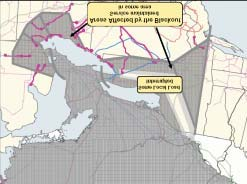
\includegraphics[width=\linewidth]{figures/chapter05/fig5_0a_blackout_area.jpg}}}
 \end{minipage}}
 {右图摘自美加联合调查报告第100页图6.29\cite{blackout-final-2004}，保留原图。灰色表示事故影响区域，其中仍有部分地区保持供电；它不是逐条线路的故障传播图。}

\clearpage
事后的联合调查涉及系统认识、运行态势感知、树木清障和可靠性协调等多方面问题。\cite{blackout-release-2004}工程师需要知道的，既包括哪台设备出了问题，也包括这些设备怎样相连、哪些运行条件必须共同满足，以及连接改变之后整个系统会怎样响应。要进入这些问题，首先需要一种能够把“局部的连接”写成“整体的关系”的语言。我们在第二章学过的线性方程组，正是其中最基础的一层。

为了看清这一层结构，先把庞大的电网缩成图\ref{fig:five-grid-balance}中的四个节点、五条线路，并用理想直流电路的节点电流平衡作教学模型。这里不复原事故电网，也暂不处理交流电网的完整运行条件。每条线路先规定一个参考方向，电流按这个方向记正，反向记负；在不积累电荷的连接点，\textbf{外部注入的电流加上线路流入，必须等于线路流出}。把各节点的这条关系分别写出来，就得到一组线性方程。

\FiveIntroFigure{从网络连接到节点方程：每一条线路同时联系两个节点。}
 {fig:five-grid-balance}{%
 \begin{tikzpicture}[x=1cm,y=1cm,font=\small]
  \node[fivenode] (n1) at (1.0,2.2) {1};
  \node[fivenode] (n2) at (3.6,3.9) {2};
  \node[fivenode] (n3) at (3.6,.5) {3};
  \node[fivenode] (n4) at (6.2,2.2) {4};
  \draw[fiveflow] (n1)--node[above left] {$f_1$} (n2);
  \draw[fiveflow] (n1)--node[below left] {$f_2$} (n3);
  \draw[fiveflow] (n2)--node[left] {$f_3$} (n3);
  \draw[fiveflow] (n2)--node[above right] {$f_4$} (n4);
  \draw[fiveflow] (n3)--node[below right] {$f_5$} (n4);
  \draw[-{Stealth[length=2mm]},FiveGreen,line width=1pt] (-.1,2.2)--(n1);
  \node[align=center,text=FiveGreen] at (.45,1.25) {外部\mbox{注入}};
  \draw[-{Stealth[length=2mm]},FiveGreen,line width=1pt] (n4)--(7.3,2.2);
  \node[align=center,text=FiveGreen] at (6.8,1.25) {外部\mbox{取出}};
  \draw[fiveguide] (7.75,.1)--(7.75,4.6);
  \node[text=FiveInk,font=\bfseries] at (11.0,4.55) {把节点2单独取出来};
  \node[fivenode,draw=FiveRose] (zoom) at (11.0,2.4) {2};
  \draw[fiveflow] (8.8,2.4)--node[above] {$f_1$} (zoom);
  \draw[fiveflow] (zoom)--node[above] {$f_4$} (13.2,2.4);
  \draw[fiveflow] (zoom)--node[right] {$f_3$} (11.0,.6);
  \draw[-{Stealth[length=2mm]},FiveGreen,line width=1pt]
   (11.0,3.9)--node[right] {$b_2$} (zoom);
  \node[align=center,text=FiveRose] at (11.0,-.1)
   {$b_2+f_1=f_3+f_4$};
 \end{tikzpicture}}
 {图中方向只是符号约定，不预先限制电流的实际方向。放大图取 $b_2$ 为外部净注入；它为负时表示该节点向外取出电流。所有连接均为自拟教学示意。}

例如节点2的关系是 $-f_1+f_3+f_4=b_2$。设 $\boldsymbol f$ 收集五条线路的电流，$\boldsymbol b$ 收集四个节点的外部净注入，把全网的节点方程合在一起，就写成
\begin{equation}
 A\boldsymbol f=\boldsymbol b.
 \label{eq:five-grid-balance}
\end{equation}
这里的 $A$ 是一个 $4\times5$ 的\term{incidence-matrix}：每列对应一条线路，在流出节点所在行记 $+1$，在流入节点所在行记 $-1$，其余位置记 $0$。它只记录谁与谁相连，以及我们怎样约定方向。设备的名称与地理位置暂时隐去，网络的连接关系却完整地留在了数表中。电网络的这种组织方式，也是用线性代数研究网络结构的经典入口。\cite{strang-networks-2011}

但是，写出方程还不是问题的终点。给定一组外部供需，每条线路的电流都能算出来吗？如果能，是否只有一种满足节点平衡的分配？把所有节点方程相加，会不会发现有些条件早已包含在其余条件之中？第二章的消元法可以帮助我们作出判断；本章则要继续解释：\textbf{这些判断为什么成立，它们究竟反映了网络中的什么结构？}

\clearpage
先看供需。并不是任意写下一组节点净注入，都能由内部线路实现；在这个连通的教学网络中，全网注入与取出必须平衡。能够实现的 $\boldsymbol b$ 组成 $A$ 的\term{column-space}。再看线路：沿一个闭合回路同时增加一股循环电流，各节点都多流入一份、也多流出一份，外部收支因而不变。这类满足 $A\boldsymbol z=\boldsymbol0$ 的变化，属于 $A$ 的\term{null-space}。\textbf{一个空间回答“什么目标能够达到”，另一个空间回答“达到同一目标还留下什么自由度”。}

\FiveIntroFigure{同一张网络引出的四个问题：四个基本子空间各有工程含义。}
 {fig:five-grid-four-questions}{%
 \begin{tikzpicture}[x=1cm,y=1cm,font=\small]
  \foreach \xx/\yy in {0/4.65,7.65/4.65,0/0,7.65/0}{
   \draw[fivecard] (\xx,\yy) rectangle ++(7.1,4.3);
  }
  % 列空间：外部收支由内部线路实现。
  \begin{scope}[shift={(0,4.65)}]
   \node[font=\bfseries,text=FiveBlue] at (3.55,3.85) {列空间：哪些供需能够实现？};
   \foreach \name/\x/\y in {a/1.4/1.9,b/3.4/2.85,c/3.4/.95,d/5.4/1.9}
    \coordinate (\name) at (\x,\y);
   \foreach \s/\t in {a/b,a/c,b/c,b/d,c/d}
    \draw[fiveflow] (\s)--(\t);
   \foreach \name in {a,b,c,d}\fill[FiveBlue] (\name) circle (2.5pt);
   \draw[-{Stealth[length=2mm]},FiveGreen,line width=1.1pt] (.3,1.9)--(a);
   \draw[-{Stealth[length=2mm]},FiveGreen,line width=1.1pt] (d)--(6.5,1.9);
   \node[text=FiveGreen] at (.7,1.25) {注入};
   \node[text=FiveGreen] at (6.1,1.25) {取出};
   \node at (3.55,.38) {寻找满足节点平衡的线路电流};
  \end{scope}
  % 零空间：有符号回路向量，逆着f2增加电流。
  \begin{scope}[shift={(7.65,4.65)}]
   \node[font=\bfseries,text=FiveRose] at (3.55,3.85) {零空间：哪些循环不改变收支？};
   \coordinate (a) at (1.4,1.9);\coordinate (b) at (3.4,2.85);
   \coordinate (c) at (3.4,.95);\coordinate (d) at (5.4,1.9);
   \draw[fiveguide] (b)--(d)--(c);
   \draw[fivecycle] (a)--node[above left] {$t$} (b);
   \draw[fivecycle] (b)--node[right] {$t$} (c);
   \draw[fivecycle] (c)--node[below left] {$t$} (a);
   \foreach \name in {a,b,c,d}\fill[FiveInk] (\name) circle (2.5pt);
   \node[align=center,text=FiveRose,font=\footnotesize] at (5.6,2.95) {每个节点\\一进一出};
   \node at (3.55,.38) {线路记录变了，节点净收支未变};
  \end{scope}
  % 行空间：电势差为A^T v；使用同一网络。
  \begin{scope}[shift={(0,0)}]
   \node[font=\bfseries,text=FiveBlue] at (3.55,3.85) {行空间：电势差从哪里来？};
   \node[fivenode] (a) at (1.4,1.9) {$v_1$};
   \node[fivenode] (b) at (3.4,2.85) {$v_2$};
   \node[fivenode] (c) at (3.4,.95) {$v_3$};
   \node[fivenode] (d) at (5.4,1.9) {$v_4$};
   \foreach \s/\t in {a/c,b/c,b/d,c/d}\draw[fiveguide] (\s)--(\t);
   \draw[fiveflow] (a)--node[above left,font=\footnotesize] {$v_1-v_2$} (b);
   \node at (3.55,.38) {节点电势决定线路两端的电势差};
  \end{scope}
  % 左零空间：内部流动抵消，留下整体约束。
  \begin{scope}[shift={(7.65,0)}]
   \node[font=\bfseries,text=FiveGreen] at (3.55,3.85) {左零空间：全网受什么约束？};
   \draw[fiveguide,rounded corners=10pt] (1.05,.72) rectangle (6.0,3.15);
   \coordinate (a) at (1.7,1.95);\coordinate (b) at (3.5,2.75);
   \coordinate (c) at (3.5,1.15);\coordinate (d) at (5.3,1.95);
   \foreach \s/\t in {a/b,a/c,b/c,b/d,c/d}\draw[fiveflow,FiveGray!60] (\s)--(\t);
   \foreach \name in {a,b,c,d}\fill[FiveGray] (\name) circle (2.5pt);
   \draw[-{Stealth[length=2mm]},FiveGreen,line width=1.1pt] (.2,1.95)--(a);
   \draw[-{Stealth[length=2mm]},FiveGreen,line width=1.1pt] (d)--(6.8,1.95);
   \node[fill=white,inner sep=2pt,font=\footnotesize] at (3.5,1.95) {内部一进一出相抵消};
   \node at (3.55,.38) {把各节点合起来，外部收支必须平衡};
  \end{scope}
 \end{tikzpicture}}
 {四幅图使用同一连接结构。上右图画的是相对于某个已有平衡方案的电流增量，$t>0$ 时沿红色箭头循环；它不表示无电源的电阻回路会自行维持电流。此处只预览结构，严格定义与相互关系将在本章正文中展开。}

还有另一种观察方式：把各节点的电势排成向量 $\boldsymbol v$，每条线路两端的电势差便组成 $A^{\mathrm T}\boldsymbol v$。这些能够由节点电势产生的线路记录，组成 $A$ 的\term{row-space}。而把全部节点方程相加，内部线路一进一出全部抵消，只留下 $b_1+b_2+b_3+b_4=0$；这条整体约束来自 $A$ 的\term{left-null-space}。甚至把所有节点电势同时加上一个相同的数，线路电势差也完全不变，这同样体现了转置矩阵的零空间。\cite{strang-networks-2011}

第三章从转置中引出的\term{fundamental-subspaces}，现在各有了具体的工程问题。列空间与左零空间联系节点端的“能够实现”与“必须满足”，行空间与零空间联系线路端的“电势差”与“循环自由度”。四个名称背后，是同一个工程系统的四种关系。节点守恒只给出了其中一层条件；线路实际怎样分配电流，还要结合元件关系。\textbf{本章的目标，正是把“方程有没有解、解是否唯一、所有解如何组成”组织成对这些关系的整体认识。}

\clearpage
真实电网也不会停在同一时刻。用电需求随时间变化，设备会接入或退出；在今天的电力系统中，储能装置还会把某个时段充入的能量留到另一个时段使用，以帮助调节供需。\cite{doe-storage-grid}一张满足节点平衡的记录，只说明此刻的关系。工程师还需要连续地记录状态，追问下一时刻会怎样，以及一次变化会怎样影响之后的运行。

\FiveIntroFigure{从一张快照到连续记录：平衡关系描述此刻，更新规则联系前后。}
 {fig:five-grid-state-sequence}{%
 \begin{tikzpicture}[x=1cm,y=1cm,font=\small]
  \foreach \xx/\kk in {0/k,5.15/{k+1},10.3/{k+2}}{
   \begin{scope}[shift={(\xx,0)}]
    \draw[fivecard] (0,0) rectangle (4.1,3.15);
    \node[font=\bfseries,text=FiveBlue] at (2.05,2.73) {时刻 $\kk$};
    \coordinate (a) at (.75,1.62);\coordinate (b) at (2.0,2.13);
    \coordinate (c) at (2.0,1.11);\coordinate (d) at (3.25,1.62);
    \foreach \s/\t in {a/b,a/c,b/c,b/d,c/d}\draw[FiveGray!55,line width=.6pt] (\s)--(\t);
    \foreach \name in {a,b,c,d}\fill[FiveBlue] (\name) circle (2.2pt);
    \node[text=FiveRose] at (2.05,.55) {状态记录 $\boldsymbol x_{\kk}$};
   \end{scope}}
  \draw[fivecycle] (4.15,1.6)--node[above,font=\footnotesize] {更新} (5.1,1.6);
  \draw[fivecycle] (9.3,1.6)--node[above,font=\footnotesize] {更新} (10.25,1.6);
  \draw[fiveguide] (.25,-.42)--(14.15,-.42);
  \node[fill=white,text=FiveGray] at (7.2,-.42)
   {连续记录同一个系统，才能讨论它随时间怎样变化};
 \end{tikzpicture}}
 {这里仅示意状态记录的先后次序，没有指定真实电网的参数或演化曲线。连接固定时，状态仍可能变化；连接改变时，模型也需要随之更新。}

例如，储能装置下一时段的电量，等于当前电量加上本时段的净充入量。把需要记住的量有序排成一列，就得到\term{state-vector}。若某个教学模型在所考察范围内可用固定的线性更新规则描述，并暂不考虑外部输入，状态之间便可以写成
\begin{equation}
 \boldsymbol x_{k+1}=F\boldsymbol x_k.
 \label{eq:five-state-preview}
\end{equation}
这里 $F$ 是\term{state-transition-matrix}，它记录从当前状态到下一状态的作用；前面的 $A$ 则记录节点与线路的连接。两种矩阵承担不同任务。真实系统的完整动态模型通常更复杂，式\eqref{eq:five-state-preview}只为后面的离散递推选读打开入口：\textbf{同一个矩阵反复作用，怎样把一个初始状态带向之后的一串状态？}

于是，从电网中提出的问题便有了次序：先辨认哪些平衡可以实现，再说明达到同一平衡可以保留哪些自由度，进而把行与列、矩阵与转置联系起来；在此基础上，再观察状态怎样随时间更新。我们不会在本章用一个小矩阵重演北美大停电，但可以开始读懂大型系统背后的基本关系。百余年来，从街区里的电灯到跨地区的互联网络，人类建造的不只是更多设备，也是一套越来越复杂的相互联系。\textbf{本章就从方程的全部解出发，学习看清这份联系的结构。}

\par\clearpage
\endgroup
\setcounter{figure}{0}
% CHAPTER 5 INTRODUCTION END
% 后续5.1及各节正文待编写；保留章首介绍性实例。

% --- 第 6 章 ---
\chapter{行列式：从体积到可逆性}
\label{chap:determinants}
% 在这里编写本章正文。

% --- 第 7 章 ---
\chapter{内积空间与正交性：线性空间中的几何}
\label{chap:inner-products}
% 在这里编写本章正文。

% --- 第 8 章 ---
\chapter[特征空间与相似变换：寻找最自然的坐标系]{特征空间与相似变换：\\寻找最自然的坐标系}
\label{chap:eigenspaces}
% 在这里编写本章正文。

% --- 第 9 章 ---
\chapter{矩阵对角化：寻找最简单的表示}
\label{chap:diagonalization}
% 在这里编写本章正文。

% --- 第 10 章 ---
\chapter{二次型：从矩阵到几何形状}
\label{chap:quadratic-forms}
% 在这里编写本章正文。

% --- 第 11 章（选读） ---
\chapter{奇异值分解：数据中的主方向（选读）}
\label{chap:svd}
% 在这里编写本章正文。

% ============================================================
% 后记：承接第十一章，作为全书正文的叙事收束；附录与工具性材料随后。
% 按用户原文保留全部原句，补充三处过渡；正文共1072字（不计空白，含标点）。
\begingroup
\catcode`。=12 \catcode`，=12 \catcode`：=12 \catcode`；=12
\catcode`？=12 \catcode`！=12 \catcode`（=12 \catcode`）=12
\ctexset{chapter={
    format=\centering,
    titleformat=\fontsize{30pt}{38pt}\selectfont\heavykaishu\color{LogicColor},
    beforeskip=0pt,afterskip=10pt
}}
\chapter*{后记}
\markboth{后记}{后记}
\addcontentsline{toc}{chapter}{后记}
\linespread{1}\fontsize{11.5pt}{17.5pt}\selectfont
\setlength{\parindent}{2em}
\setlength{\parskip}{1pt}
\clubpenalty=10000 \widowpenalty=10000

\noindent\textbf{我们从一个笼子里的鸡和兔开始。}

头 35 个，脚 94 只。这是小学奥数里最朴素的问题，两个未知数，两个方程，用最原始的消元思想就能算出答案。那时，草稿纸上的每一次涂改，都只是为了让头数与脚数相合。我们尚不知道，一个朴素的办法，也会成为跨越时代的共同语言。

一千五百年后，洛斯阿拉莫斯的科学家们抱着同样的思路，在机械台式计算器上求解上百阶的方程组，为核反应堆的临界计算提供了关键数据。第一台通用电子计算机 ENIAC 建成后，最早的核心任务之一，也是求解大型线性方程组。从鸡兔同笼到核反应堆，中间横着的，是一条人类理性踩出来的漫长道路。

纸上的筹算、桌边的摇柄、机房里的灯光，属于不同的年代；被一次次传下来的，却是把问题说清、把关系列出、把未知逐步求出的耐心。

线性代数从来不是一套凭空造出来的符号游戏。它诞生于工程的需求，成长于抽象的思维，最终成为了现代科学的通用语言。从原子弹到登月火箭，从跨海大桥到人工智能，几乎所有伟大的工程背后，都立着它的骨架。

你或许曾觉得，这门课里的定义、定理、公式，只是为了考试而存在。但你回头看看自己走过的路：你学会了用向量描述世界，用消元法拆解方程组，用矩阵组织运算，用线性变换理解结构，用秩与解空间把握存在与唯一，用行列式度量体积与可逆，用特征值寻找系统的固有方向。这些概念从来不是孤立的知识点，它们是同一棵树上的枝干，根植于同一个思想：线性结构，是这个世界最普遍、最简洁、最有力的描述方式之一。

这就是人类理性的力量。我们从具体的问题出发，靠着逻辑与抽象，一步步走向普遍的规律，再反过来支撑起更宏大的创造。数学是这个过程最纯粹的形式，而线性代数，是这个形式最基础的语法。

如今，这份耐心也来到你的书桌前。一次重算，一处改正，一段终于读懂的推导，都让前人的积累成为你能够亲自使用的知识。

你不需要记住每一个定理的证明，也不需要熟练手算每一个矩阵的化简。真正重要的是，你开始拥有了一种眼光 —— 一种在纷繁复杂中看见线性骨架的眼光。这种眼光会让你在未来的任何领域里，都比别人多一层理解。

所以，当你合上这本书的时候，不要觉得线性代数已经结束了。你只是刚刚开始。后面的路还很长，有更广阔的空间等待你去探索，有更复杂的系统等待你去理解，有更深刻的问题等待你去回答。但无论你走到哪里，你都会发现，这里的每一个概念 —— 向量、矩阵、秩、维数、特征值 —— 都还在那里，安静地、精确地、充满力量地支撑着你眼前的一切。

而你刚刚走完的，就是这段最伟大的理性之路的第一步。

愿你在未来的某个时刻，忽然想起这本书里的某一个概念，发现它正在你眼前的某个系统里安静地运转。

\par\clearpage
\endgroup

% ============================================================
% 附录 A：复数。原创文字与 TikZ 配图；沿用参考模板的定义、定理与例题模块。
% ============================================================
\appendix
\begingroup
\catcode`。=12 \catcode`，=12 \catcode`：=12 \catcode`；=12
\catcode`？=12 \catcode`！=12 \catcode`（=12 \catcode`）=12
\ctexset{
    chapter={name={附录\space,},number=\Alph{chapter},afterskip=25pt},
    section={format=\raggedright\Large\bfseries\color{MainText},beforeskip=20pt,afterskip=12pt},
    subsection={format=\raggedright\normalsize\bfseries,beforeskip=14pt,afterskip=8pt}
}
\chapter{复数：从数轴走向平面}
\label{app:complex}
\linespread{1}\fontsize{12pt}{20pt}\selectfont
\setlength{\parindent}{2em}\setlength{\parskip}{4pt}
\setlength{\abovedisplayskip}{9pt}\setlength{\belowdisplayskip}{9pt}
\clubpenalty=10000 \widowpenalty=10000
\tcbset{commonbox/.append style={breakable=false,
    fontupper=\linespread{1}\fontsize{11.5pt}{18pt}\selectfont,
    before skip=14pt,after skip=12pt}}
\definecolor{ComplexBlue}{HTML}{397AA1}
\definecolor{ComplexRose}{HTML}{AC4963}
\definecolor{ComplexGreen}{HTML}{448678}
\definecolor{ComplexGray}{HTML}{6A747B}
\tikzset{
    cxaxis/.style={-{Stealth[length=2mm]},thin,ComplexGray},
    cxblue/.style={-{Stealth[length=2.5mm]},line width=1.2pt,ComplexBlue},
    cxrose/.style={-{Stealth[length=2.5mm]},line width=1.2pt,ComplexRose},
    cxgreen/.style={-{Stealth[length=2.5mm]},line width=1.2pt,ComplexGreen},
    cxguide/.style={densely dashed,ComplexGray!65,thin}
}
\captionsetup[figure]{font=small,labelfont=bf,skip=7pt}
\renewcommand{\thefigure}{\thechapter.\arabic{figure}}
\newcommand{\complexfigure}[3]{%
    \par\addvspace{7pt}\noindent\begin{minipage}{\linewidth}
        \centering #3\par\captionof{figure}{#1}\label{#2}
    \end{minipage}\par\addvspace{7pt}}

在实数范围内，方程 $x^2+1=0$ 没有解。但“没有实数解”并不意味着只能止步于此：我们可以扩充所用的数，让这个方程也有可讨论的解。正如从二维走向高维时保留向量的运算规则，从实数走向复数时，我们也希望保留熟悉的加法、乘法与分配律。

这次扩充还有一份几何上的收获：实数在数轴上表示位置，复数在平面上同时记录两个坐标；加法仍是位移的合成，乘法却能把伸缩与旋转合在一起。\textbf{先在平面上看清位置，再在运算中辨认结构。}本附录沿着复数及其运算、共轭与模、极式与旋转的线索展开，重点说明欧拉公式如何把一条代数等式变成一幅单位圆图景。

\section{扩充数系：从一个新单位开始}

实数的平方总是非负，因此我们引入一个新单位 $i$，规定 $i^2=-1$。这样，$i$ 与 $-i$ 都满足 $x^2+1=0$。新符号的意义不在于它能不能画在实数轴上，而在于怎样给它建立一致的运算规则。

\begin{definition}[复数及其实部、虚部]
满足 $i^2=-1$ 的 $i$ 称为\textbf{\term{imaginary-unit}}。形如
\[
    z=a+bi,\qquad a,b\in\mathbb R
\]
的数称为\textbf{\term{complex-number}}。其中 $a$ 称为\textbf{\term{real-part}}，$b$ 称为\textbf{\term{imaginary-part}}，分别记为 $\operatorname{Re}z=a$、$\operatorname{Im}z=b$。复数全体记为 $\mathbb C$。

两个复数相等，当且仅当它们的实部与虚部分别相等。
\end{definition}

例如，$z=2-3i$ 的实部为2，虚部为 $-3$；虚部是实数 $-3$，不是 $-3i$。当 $b=0$ 时，$a+0i$ 就是实数 $a$，所以 $\mathbb R\subset\mathbb C$。当 $a=0$ 且 $b\ne0$ 时，$bi$ 称为\term{pure-imaginary}。

第1章已经提到复数域：它不是把实数运算推翻，而是在更大的数系中继续使用这些运算。这里的 $i$ 是数，不是向量下标，也不是实数范围内存在的某个平方根。连续相乘可得
\[
    i^0=1,\qquad i^1=i,\qquad i^2=-1,\qquad i^3=-i,\qquad i^4=1.
\]
再乘 $i$，又从这一循环开始。稍后我们会看到，这四个值恰好对应单位圆上每次转过四分之一周的位置。

\section{分部相加，依律相乘}

两个复数相加，就是实部与实部相加、虚部与虚部相加。例如，$(2+i)+(1+2i)=3+3i$。这个规则与平面向量逐个分量相加完全一致。相减也如此，先把实部与虚部分开，再分别计算。

\begin{property}[复数的加法、减法与乘法]
设 $z=a+bi$、$w=c+di$，则
\[
\begin{aligned}
    z+w&=(a+c)+(b+d)i,\\
    z-w&=(a-c)+(b-d)i,\\
    zw&=(ac-bd)+(ad+bc)i.
\end{aligned}
\]
乘法按分配律展开，再把 $i^2$ 换成 $-1$。这些运算满足熟悉的交换律、结合律与分配律。
\end{property}

\begin{example}[展开以后，只留下两部分]
计算 $(2+i)(1+2i)$。按分配律，
\[
    (2+i)(1+2i)=2+4i+i+2i^2=5i.
\]
实部相消，虚部合并。复数乘法不等于把两个坐标分别相乘：若错误地把 $(2,1)$ 与 $(1,2)$ 的对应分量相乘，就得不到这里的结果。
\end{example}

加法对应怎样的图形？把复数 $a+bi$ 放在平面中的点 $(a,b)$ 上，再从原点画出箭头，原来的平行四边形定则便直接适用。

\complexfigure{复数加法与向量加法使用同一幅图：从 $z$ 的终点接上代表 $w$ 的箭头，得到 $z+w$。}{fig:complex-addition}{%
\begin{tikzpicture}[scale=1.05,font=\small]
    \draw[cxaxis] (-.5,0)--(4.3,0) node[right] {$\operatorname{Re}$};
    \draw[cxaxis] (0,-.35)--(0,3.8) node[above] {$\operatorname{Im}$};
    \draw[cxblue] (0,0)--(2,1) node[midway,below] {$z=2+i$};
    \draw[cxgreen] (0,0)--(1,2) node[midway,left] {$w=1+2i$};
    \draw[cxgreen,dashed] (2,1)--(3,3);
    \draw[cxguide] (1,2)--(3,3);
    \draw[cxrose] (0,0)--(3,3) node[above right] {$z+w=3+3i$};
    \node[below left] at (0,0) {$O$};
\end{tikzpicture}}

\section{共轭看镜像，模长看距离}

\term{complex-plane}正是上述表示复数的平面：横坐标记录实部，横轴称为\term{real-axis}；纵坐标记录虚部，纵轴称为\term{imaginary-axis}。复数是数，平面上的点与箭头是它的几何表示。有了这层对应，我们便能用对称与距离理解两个新的概念。

\begin{definition}[共轭与模]
对 $z=a+bi$，复数
\[
    \overline z=a-bi
\]
称为 $z$ 的\textbf{\term{conjugate}}；非负实数
\[
    |z|=\sqrt{a^2+b^2}
\]
称为 $z$ 的\textbf{\term{modulus}}。
\end{definition}

共轭只把虚部变号，因此将点 $(a,b)$ 映到 $(a,-b)$，是关于实轴的镜像；模只问离原点多远，是勾股定理给出的长度。图\ref{fig:complex-conjugate}以 $a,b>0$ 示意，其他象限的解释相同。

\complexfigure{共轭的镜像关系。$z=a+bi$ 与 $\overline z=a-bi$ 关于实轴对称，到原点的距离相同，因此 $|\overline z|=|z|$。}{fig:complex-conjugate}{%
\begin{tikzpicture}[scale=1.05,font=\small]
    \draw[cxaxis] (-.65,0)--(4.8,0) node[right] {$\operatorname{Re}$};
    \draw[cxaxis] (0,-2.5)--(0,2.55) node[above] {$\operatorname{Im}$};
    \draw[cxguide] (0,1.6)--(2.6,1.6)--(2.6,-1.6)--(0,-1.6);
    \draw[cxblue] (0,0)--(2.6,1.6) node[midway,above left] {$|z|$};
    \draw[cxrose] (0,0)--(2.6,-1.6) node[midway,below left] {$|\overline z|$};
    \fill[ComplexBlue] (2.6,1.6) circle (2pt) node[above right] {$z=a+bi$};
    \fill[ComplexRose] (2.6,-1.6) circle (2pt) node[below right] {$\overline z=a-bi$};
    \draw[<->,ComplexGray] (3.5,1.35)--(3.5,-1.35);
    \node[text=ComplexGray,anchor=west] at (3.7,.45) {镜像};
    \node[below left] at (0,0) {$O$};
    \node[above left] at (2.6,0) {$a$};
    \node[left] at (0,1.6) {$b$};
    \node[left] at (0,-1.6) {$-b$};
\end{tikzpicture}}

共轭也使除法变得方便。因为
\[
    z\overline z=(a+bi)(a-bi)=a^2+b^2=|z|^2,
\]
分母乘上其共轭，就变成了实数。若 $w=c+di\ne0$，则 $c^2+d^2>0$，从而
\[
    \frac zw
    =\frac{z\overline w}{w\overline w}
    =\frac{ac+bd}{c^2+d^2}+\frac{bc-ad}{c^2+d^2}i.
\]
这里的条件 $w\ne0$ 不能省略。每个非零复数都有倒数，因而除法的结果仍在 $\mathbb C$ 中。

\begin{example}[用共轭消去分母的虚部]
\[
    \frac{2+i}{1-i}
    =\frac{(2+i)(1+i)}{(1-i)(1+i)}
    =\frac{1+3i}{2}=\frac12+\frac32i.
\]
分子与分母必须同时乘 $1+i$，这才保持原来的商不变。
\end{example}

\begin{property}[共轭与模的常用关系]
对任意复数 $z,w$，有
\[
\begin{aligned}
    \overline{\overline z}&=z,&\overline{z+w}&=\overline z+\overline w,&
    \overline{zw}&=\overline z\,\overline w,\\
    |z|&\ge0,&|z|=0&\Longleftrightarrow z=0,&|zw|&=|z|\,|w|.
\end{aligned}
\]
若 $w\ne0$，还有 $\overline{z/w}=\overline z/\overline w$、$|z/w|=|z|/|w|$。
\end{property}

前几式可以直接展开验证。模的乘法性质也有简洁依据：$|zw|^2=(zw)\overline{zw}=|z|^2|w|^2$，两边均非负，开平方即得。几何上，$|z-w|$ 表示两点之间的距离；这与实数轴上的距离公式具有相同形式。

\section{换一种坐标：模定长短，角定方向}

描述平面上的一个非原点位置，除了给出横、纵坐标，还可以先说离原点多远，再说朝哪个方向。设 $z=a+bi\ne0$，令 $r=|z|>0$，从正实轴转向向量 $Oz$ 的\term{directed-angle}为 $\theta$，则
\[
    a=r\cos\theta,\qquad b=r\sin\theta.
\]
这里的 $\theta$ 称为 $z$ 的\term{argument}。逆时针为正，顺时针为负；本附录的角度均采用弧度制。

\begin{definition}[复数的极式]
非零复数的\textbf{\term{polar-form}}为
\[
    z=r(\cos\theta+i\sin\theta),\qquad r=|z|>0.
\]
同一复数的辐角可相差 $2k\pi$，其中 $k\in\mathbb Z$。若约定 $-\pi<\theta\le\pi$，所得唯一角称为\textbf{\term{principal-argument}}，记为 $\operatorname{Arg}z$。
\end{definition}

零复数的模为0，但方向无法确定，\textbf{不定义它的辐角}。对于非零复数，判断辐角要同时看实部与虚部的正负，不能只依赖 $\tan\theta=b/a$，更不能在 $a=0$ 时作这个除法。例如，$1+i$ 与 $-1-i$ 的比值 $b/a$ 相同，方向却相差 $\pi$。

若 $z_1=r_1(\cos\alpha+i\sin\alpha)$、$z_2=r_2(\cos\beta+i\sin\beta)$，展开乘法并应用两角和公式，就得到
\[
\begin{aligned}
    z_1z_2
    &=r_1r_2\bigl[(\cos\alpha\cos\beta-\sin\alpha\sin\beta)\\
    &\hspace{30mm}+i(\sin\alpha\cos\beta+\cos\alpha\sin\beta)\bigr]\\
    &=r_1r_2\bigl[\cos(\alpha+\beta)+i\sin(\alpha+\beta)\bigr].
\end{aligned}
\]
\textbf{模相乘，辐角相加。}固定 $z_2$ 后，乘以 $z_2$ 就把原向量长度放大为 $r_2$ 倍，并绕原点旋转 $\beta$。这里的辐角相加按相差整周视为同方向理解，辐角主值的和必要时要加减 $2\pi$ 才能回到约定区间。

\complexfigure{复数乘法的极坐标解释。左图给出两个因子，右图给出乘积：长度变为 $r_1r_2$，方向角变为 $\alpha+\beta$。示意取 $r_1=1.4$、$r_2=1.5$、$\alpha=\pi/9$、$\beta=5\pi/18$。}{fig:complex-product}{%
\begin{tikzpicture}[scale=1.35,font=\small]
    \begin{scope}
        \draw[cxaxis] (-.2,0)--(2.45,0) node[right] {$\operatorname{Re}$};
        \draw[cxaxis] (0,-.2)--(0,2.4) node[above] {$\operatorname{Im}$};
        \draw[cxblue] (0,0)--(20:1.4) node[right] {$z_1$};
        \draw[cxgreen] (0,0)--(50:1.5) node[above right] {$z_2$};
        \draw[ComplexBlue,-{Stealth[length=1.3mm]}] (.55,0) arc (0:20:.55);
        \node[ComplexBlue] at (10:.8) {$\alpha$};
        \draw[ComplexGreen,-{Stealth[length=1.3mm]}] (.95,0) arc (0:50:.95);
        \node[ComplexGreen] at (37:1.15) {$\beta$};
        \node[below left] at (0,0) {$O$};
        \node[align=center] at (1.1,-.6) {两个因子\\$|z_1|=r_1,\quad |z_2|=r_2$};
    \end{scope}
    \draw[-{Stealth[length=2.5mm]},ComplexGray] (3,1.1)--(3.75,1.1)
        node[midway,above] {相乘};
    \begin{scope}[xshift=5cm]
        \draw[cxaxis] (-.2,0)--(2.3,0) node[right] {$\operatorname{Re}$};
        \draw[cxaxis] (0,-.2)--(0,2.4) node[above] {$\operatorname{Im}$};
        \draw[cxguide] (0,0)--(20:1.4);
        \draw[cxrose] (0,0)--(70:2.1) node[above right] {$z_1z_2$};
        \draw[ComplexRose,-{Stealth[length=1.5mm]}] (.65,0) arc (0:70:.65);
        \node[ComplexRose,fill=white,inner sep=1pt] at (34:1.02) {$\alpha+\beta$};
        \node[below left] at (0,0) {$O$};
        \node[align=center] at (1,-.6) {乘积\\$|z_1z_2|=r_1r_2$};
    \end{scope}
\end{tikzpicture}}

若除以一个非零复数，过程正好相反：\textbf{模相除，辐角相减}。这使乘法与除法都能读成平面上的长度变化与方向变化。

\begin{example}[乘以 $i$，为什么转过直角]
$i=\cos(\pi/2)+i\sin(\pi/2)$，模为1，辐角为 $\pi/2$。因此乘以 $i$ 不改变长度，只将向量逆时针转过直角。代数上也能看到同一件事：
\[
    i(a+bi)=-b+ai,\qquad (a,b)\longmapsto(-b,a).
\]
例如点 $(2,1)$ 对应 $2+i$，乘以 $i$ 后变成 $-1+2i$，对应点 $(-1,2)$。
\end{example}

\section{欧拉公式：把旋转写成指数}

在所有非零复数中，模为1的情形最能单独显出方向。满足 $|z|=1$ 的点构成\term{unit-circle}。单位圆上的一个点转过角 $\theta$ 后，其横坐标是 $\cos\theta$，纵坐标是 $\sin\theta$，所以这个点对应的复数为 $\cos\theta+i\sin\theta$。

\begin{theorem}[欧拉公式]
对任意实数 $\theta$，有\textbf{\term{euler}}：
\begin{equation}\label{eq:complex-euler}
    \boxed{e^{i\theta}=\cos\theta+i\sin\theta.}
\end{equation}
因此 $|e^{i\theta}|=1$，而 $\theta$ 是它的一个辐角。
\end{theorem}

读这条公式时，可以暂时把右侧看作“点的坐标”，把左侧看作“转过的角度”。它们描述的是同一个单位圆上的位置。指数中的 $i$ 使角度进入复数运算，而模始终保持为1。

\complexfigure{欧拉公式的单位圆图景。从 $1$ 沿单位圆逆时针转过 $\theta$，到达 $e^{i\theta}$；点的两个坐标分别是 $\cos\theta$ 与 $\sin\theta$。虚线显示投影，圆弧显示旋转方向。图中示意 $0<\theta<\pi/2$，公式对所有实数角成立。}{fig:complex-euler}{%
\begin{tikzpicture}[scale=2.55,font=\small]
    \fill[ComplexBlue!4] (0,0) circle (1);
    \draw[ComplexGray!70,thin] (0,0) circle (1);
    \draw[cxaxis] (-1.35,0)--(1.5,0) node[right] {$\operatorname{Re}$};
    \draw[cxaxis] (0,-1.28)--(0,1.4) node[above] {$\operatorname{Im}$};
    \coordinate (P) at (52:1);
    \draw[cxguide] (P)--({cos(52)},0);
    \draw[cxguide] (P)--(0,{sin(52)});
    \draw[ComplexBlue,line width=1.8pt] (0,0)--({cos(52)},0);
    \draw[ComplexGreen,line width=1.8pt] ({cos(52)},0)--(P);
    \draw[cxrose] (0,0)--(P);
    \draw[ComplexRose,line width=1.2pt,-{Stealth[length=2.2mm]}] (1,0) arc (0:52:1);
    \draw[ComplexGray,-{Stealth[length=1.3mm]}] (.25,0) arc (0:52:.25);
    \node at (26:.38) {$\theta$};
    \fill[ComplexRose] (P) circle (.022);
    \node[above right,align=left] at (P) {$e^{i\theta}$\\$=\cos\theta+i\sin\theta$};
    \node[below,text=ComplexBlue] at (.32,-.03) {$\cos\theta$};
    \node[right,text=ComplexGreen,fill=white,inner sep=1pt] at (.66,.37) {$\sin\theta$};
    \node[above left] at (0,1) {$i$};
    \node[below right] at (1,0) {$1$};
    \node[above left] at (-1,0) {$-1$};
    \node[below left] at (0,-1) {$-i$};
    \node[below left] at (0,0) {$O$};
    \node[text=ComplexGray] at (-.48,-.53) {$|z|=1$};
\end{tikzpicture}}

为什么左边可以使用指数记号？第1章选读曾用有限项多项式近似 $e^t$。若把这种展开延伸为无限项，就可以定义\term{complex-exp}：
\[
    e^w=\sum_{k=0}^{\infty}\frac{w^k}{k!}.
\]
这个展开对每个复数 $w$ 都\term{absolute-convergence}，即各项的模相加仍有有限的和，因而可以按奇数次幂、偶数次幂重新分组。代入 $w=i\theta$，利用 $i^2=-1$，得到
\[
\begin{aligned}
    e^{i\theta}
    &=\left(1-\frac{\theta^2}{2!}+\frac{\theta^4}{4!}-\cdots\right)\\
    &\quad+i\left(\theta-\frac{\theta^3}{3!}+\frac{\theta^5}{5!}-\cdots\right)\\
    &=\cos\theta+i\sin\theta.
\end{aligned}
\]
最后一行使用了正弦、余弦各自的展开。这是欧拉公式的一个来源；尚未学习无穷展开的读者可以把这一段作为选读，先掌握单位圆上的坐标含义。

\textbf{长度留给模，方向交给角。}借助欧拉公式，极式变成更紧凑的\term{exponential-form}
\[
    z=re^{i\theta},\qquad
    (r_1e^{i\alpha})(r_2e^{i\beta})=r_1r_2e^{i(\alpha+\beta)}.
\]
当 $r_2=1$ 时，这就是纯粹的\term{rotation}：角度增加 $\beta$，长度保持不变。任取实数 $a,\theta$，还可写成 $e^{a+i\theta}=e^a(\cos\theta+i\sin\theta)$，其中实部 $a$ 控制模，虚部 $\theta$ 控制方向。

把几个熟悉的角代入，可以把公式与图上的四个方向一一对应：
\[
    e^{i0}=1,\qquad e^{i\pi/2}=i,\qquad
    e^{i\pi}=-1,\qquad e^{i3\pi/2}=-i.
\]
尤其是 $e^{i\pi}+1=0$，它在单位圆上说的只是：从1转过半周，就到达 $-1$。漂亮的等式背后，是一个明确的几何动作。

\begin{example}[让屏幕上的方向标记转过四分之一周]
把屏幕平面中的一个方向标记用复数 $z=2+i$ 表示。若希望绕原点逆时针旋转 $\pi/2$，可直接乘 $e^{i\pi/2}=i$，得到
\[
    z'=iz=-1+2i.
\]
原来与现在的模都为 $\sqrt5$。这里仅把复数作为平面坐标的计算工具；实际屏幕若采用向下为正的纵轴，需要先统一坐标约定。
\end{example}

\section{反复旋转：乘方与开方}

一次乘法使辐角相加，多次相乘便使角度逐次累积。这把原本可能很长的代数展开，变成了“模的乘方”与“角的倍乘”。

\begin{theorem}[棣莫弗定理]
对实数 $\theta$ 与整数 $n$，\textbf{\term{demoivre}}给出
\[
    (\cos\theta+i\sin\theta)^n
    =\cos(n\theta)+i\sin(n\theta).
\]
因而对非零复数 $z=r(\cos\theta+i\sin\theta)$，有
\[
    z^n=r^n\bigl(\cos(n\theta)+i\sin(n\theta)\bigr).
\]
\end{theorem}

对正整数 $n$，反复使用“模相乘、辐角相加”即可得到；$n=0$ 时两边都是1，负整数情形再取倒数。非零条件保证负整数次幂有意义。例如，$1+i=\sqrt2e^{i\pi/4}$，所以
\[
    (1+i)^4=(\sqrt2)^4e^{i\pi}=-4.
\]
我们没有逐项展开四次方，而是看见：长度先取四次方，方向角再转到原来的四倍。

反过来，若已知 $z$，要求 $w^n=z$，就是求\term{nth-root}。设 $z=re^{i\theta}\ne0$，$n$ 为正整数，则全部根为
\[
    w_k=r^{1/n}e^{i(\theta+2k\pi)/n},\qquad k=0,1,\ldots,n-1.
\]
它们有相同的模，辐角依次相差 $2\pi/n$，因此均匀分布在同一个圆上。加上 $2k\pi$ 的步骤不能省略：原来代表同一方向的不同角，在除以 $n$ 后会产生不同的根。若 $z=0$，则只有根 $w=0$。

特别地，方程 $w^n=1$ 的解称为\term{roots-unity}。下面以四次单位根为例，看见乘以 $i$ 与四次开方之间的联系。

\complexfigure{四次单位根 $1,i,-1,-i$ 均匀分布在单位圆上。每次乘以 $i$ 都逆时针转过 $\pi/2$，四次以后回到原处。}{fig:complex-roots}{%
\begin{tikzpicture}[scale=2,font=\small]
    \draw[ComplexGray!65] (0,0) circle (1);
    \draw[cxaxis] (-1.4,0)--(1.45,0) node[right] {$\operatorname{Re}$};
    \draw[cxaxis] (0,-1.4)--(0,1.45) node[above] {$\operatorname{Im}$};
    \foreach \angle in {0,90,180,270} {
        \draw[ComplexBlue!60] (0,0)--(\angle:1);
        \fill[ComplexRose] (\angle:1) circle (.027);
        \draw[ComplexGreen,-{Stealth[length=2mm]}]
            (\angle:1.13) arc (\angle:{\angle+70}:1.13);
    }
    \node[above right] at (1,0) {$1$};
    \node[above left] at (0,1) {$i$};
    \node[below left] at (-1,0) {$-1$};
    \node[below right] at (0,-1) {$-i$};
    \node at (0,0) {$O$};
    \node[ComplexGreen,fill=white,inner sep=1pt] at (45:1.34) {$\times i$};
\end{tikzpicture}}

\clearpage
\section{回到线性代数：对象可变，结构相通}

复数与平面向量有相同的两分量加法，但复数还带有自己的乘法。这个区别使我们既能把它看作平面上的位置，也能把一个固定复数看作作用于整个平面的伸缩与旋转规则。例如，固定 $c=p+qi$，定义 $T(z)=cz$，由分配律立刻有
\[
    T(z+w)=T(z)+T(w),\qquad T(tz)=tT(z)\quad(t\in\mathbb R).
\]
因此它保留了前文已经认识的线性组合关系。复数运算为“一个数怎样作用于一个平面”提供了直接例子，后续讨论线性变换时，这幅图景还会再次出现。

第1章也提醒过：谈基与维数，要先说明允许使用什么标量。\textbf{把 $\mathbb C$ 看成实向量空间时，$1,i$ 是一组基，维数为2；把它看成复向量空间时，单个向量1就是一组基，维数为1。}前者用两个实系数表示 $a+bi$，后者允许直接使用复系数 $z$，写成 $z\cdot1$。对象相同，系数范围不同，维数便随之改变。

\begin{exercise}[把运算与图形对应起来]
设 $z=1+\sqrt3i$。求 $\overline z$ 与 $|z|$，写出一个极式，并计算 $iz$、$z^3$。再在复平面上说明：哪一步是镜像，哪一步是旋转，哪一步同时改变了长度与方向？
\end{exercise}

可用以下结果核对：$\overline z=1-\sqrt3i$、$|z|=2$、$z=2e^{i\pi/3}$、$iz=-\sqrt3+i$、$z^3=-8$。共轭关于实轴镜像；乘 $i$ 保持长度、转过 $\pi/2$；三次方使模变为 $2^3$、辐角变为 $\pi$。

从 $a+bi$ 到 $re^{i\theta}$，并不是换了一个复数，而是换了描述它的方式。\textbf{代数形式便于分部运算，极坐标形式便于辨认旋转。}共轭把对称写成变号，模把距离写成平方和，欧拉公式把单位圆写成指数；不同表示相互配合，计算才有了可以看见的意义。

\par\clearpage
\endgroup

% 书末术语表：数据源 terms.tex；每次完整编译自动生成排序后的术语表.tex。
\backmatter
\begingroup
\catcode`。=12 \catcode`，=12 \catcode`：=12 \catcode`；=12
\catcode`？=12 \catcode`！=12 \catcode`（=12 \catcode`）=12
\ctexset{chapter={titleformat=\fontsize{26pt}{36pt}\selectfont\heavykaishu\color{LogicColor},afterskip=22pt}}
\chapter*{术语表}
\markboth{术语表}{术语表}
\addcontentsline{toc}{chapter}{术语表}
\linespread{1}\fontsize{11pt}{17pt}\selectfont
\setlength{\parindent}{0pt}\setlength{\parskip}{0pt}
本表按英文术语的首字母分组，组内按英文字母顺序排列，统一采用“中文术语 (English Term) [释义]”格式。条目涵盖已撰写正文与附录A的关键概念；正文只作预告的后续术语，在释义中注明相应章节。英语中的同义说法及本书采用的简称，尽量合并在同一词条中。\par\medskip
\PrintLectureGlossary
\par\clearpage
\endgroup

% 参考文献：置于全书末尾，编号供后续正文引用使用。
\begingroup
\catcode`。=12 \catcode`，=12 \catcode`：=12 \catcode`；=12
\catcode`？=12 \catcode`！=12 \catcode`（=12 \catcode`）=12
\ctexset{chapter={titleformat=\fontsize{26pt}{36pt}\selectfont\heavykaishu\color{LogicColor},afterskip=22pt}}
\renewcommand{\bibname}{参考文献}
\linespread{1}\fontsize{11pt}{17pt}\selectfont
\urlstyle{same}
\begin{thebibliography}{99}
\addcontentsline{toc}{chapter}{参考文献}
\markboth{参考文献}{参考文献}
\setlength{\itemsep}{10pt}
\setlength{\parsep}{0pt}
\renewcommand{\newblock}{\par\nobreak}
\raggedright

\bibitem{axler2024}
Axler S. \textit{Linear Algebra Done Right} (《线性代数应该这样学》)[M]. 4th ed. Cham: Springer, 2024.
\newblock \url{https://doi.org/10.1007/978-3-031-41026-0}.

\bibitem{lay2021}
Lay D C, Lay S R, McDonald J J. \textit{Linear Algebra and Its Applications}（《线性代数及其应用》）[M]. 6th ed., Global Edition. Pearson, 2021.

\bibitem{vaswani2017}
Vaswani A, Shazeer N, Parmar N, et al. Attention Is All You Need[C]//\textit{Advances in Neural Information Processing Systems}. Vol. 30. 2017: 5998--6008.
\newblock \url{https://arxiv.org/abs/1706.03762}.

\bibitem{archer2021}
Archer B J. The Los Alamos Computing Facility during the Manhattan Project[R/OL]. LA-UR-21-20164, 2021.
\newblock \url{https://arxiv.org/abs/2103.05705}.

\bibitem{openai-tokens}
OpenAI. Understanding and counting tokens[EB/OL]. OpenAI Help Center \mbox{[2026-09-25]}.
\newblock \url{https://help.openai.com/en/articles/4936856-understanding-and-counting-tokens}.

\bibitem{huggingface-tokenization}
Hugging Face. Tokenization algorithms[EB/OL]. Transformers documentation \mbox{[2026-09-25]}.
\newblock \url{https://huggingface.co/docs/transformers/tokenizer_summary}.

\bibitem{douyin-recommendation}
抖音安全与信任中心. 什么是推荐系统[EB/OL]. \mbox{[2026-09-25]}.
\newblock \url{https://trust.douyin.com/algorithm/}.

% DOUYIN CASE REFERENCES BEGIN
\bibitem{douyin-launch}
抖音安全与信任中心. 抖音安全与信任中心网站上线一周年，让信任可见、让安全可感[EB/OL]. 2026-03-30 [2026-09-26].
\newblock \url{https://95152.douyin.com/article/9171774861438144}.

\bibitem{douyin-models}
抖音安全与信任中心. 从零开始了解推荐系统[EB/OL]. 2025-03-30 [2026-09-26].
\newblock \url{https://95152.douyin.com/article/15358}.

\bibitem{douyin-behavior}
抖音安全与信任中心. 用户行为背后的算法推荐逻辑[EB/OL]. 网页标示日期2025-01-20 [2026-09-26].
\newblock \url{https://95152.douyin.com/article/15381}.

\bibitem{douyin-objectives}
抖音安全与信任中心. 抖音算法的多目标平衡[EB/OL]. 网页标示日期2025-01-20 [2026-09-26].
\newblock \url{https://95152.douyin.com/article/15383}.

\bibitem{wide-deep-2016}
Cheng H T, Koc L, Harmsen J, et al. Wide \& Deep Learning for Recommender Systems[EB/OL]. 2016 [2026-09-26].
\newblock \url{https://arxiv.org/abs/1606.07792}.

\bibitem{tfrs-two-tower}
Kula M, Chen J. Introducing TensorFlow Recommenders[EB/OL]. Google, 2020-09-23 [2026-09-26].
\newblock \url{https://blog.tensorflow.org/2020/09/introducing-tensorflow-recommenders.html}.

\bibitem{hu-als-2008}
Hu Y, Koren Y, Volinsky C. Collaborative Filtering for Implicit Feedback Datasets[C]//2008 Eighth IEEE International Conference on Data Mining. 2008: 263--272.
\newblock \url{https://yifanhu.net/PUB/cf.pdf}.

\bibitem{monolith-2022}
Liu Z, Zou L, Zou X, et al. Monolith: Real Time Recommendation System With Collisionless Embedding Table[EB/OL]. arXiv:2209.07663, 2022 [2026-09-26].
\newblock \url{https://arxiv.org/abs/2209.07663}.
% DOUYIN CASE REFERENCES END


\bibitem{eniac-photo}
作者不详. Glen Beck and Betty Snyder program the ENIAC in building 328 at the Ballistic Research Laboratory[图像/OL]. U.S. Army Photo, Wikimedia Commons \mbox{[2026-09-25]}.
\newblock \url{https://commons.wikimedia.org/wiki/File:Eniac.jpg}.

\bibitem{agc1970}
Raytheon Company. \textit{Apollo Guidance Computer Program, Block I (100) and Block II: Final Report}[R/OL]. NASA-CR-108361, SR-70-4053, 1969, sec. 2.3.1.1.
\newblock \url{https://ntrs.nasa.gov/citations/19700015154}.


\bibitem{art-linear-algebra}
Hiranabe K. \textit{The Art of Linear Algebra: Graphic Notes on ``Linear Algebra for Everyone''}[EB/OL]. With help from Gilbert Strang; 刘可方译，2023年更新。
\newblock \url{https://github.com/kenjihiranabe/The-Art-of-Linear-Algebra}.

\bibitem{hzmb-engineering}
Chan M, Leung Y W, Premaud V, et al. \textit{Challenges in Hong Kong--Zhuhai--Macao Bridge (HZMB) Hong Kong Link Road Project}[R/OL]. 项目团队技术论文，见桩帽有限元模型及荷载讨论。
\newblock \url{https://ywlgroup.com/ywl-wp/article/a04.pdf}.

\bibitem{hzmb-photo}
N509FZ. \textit{West section of Hong Kong--Zhuhai--Macau Bridge (20180902174105)}[图像/OL]. 2018-09-02. Wikimedia Commons, CC BY-SA 4.0；
\newblock \url{https://commons.wikimedia.org/wiki/File:West_section_of_Hong_Kong-Zhuhai-Macau_Bridge_(20180902174105).jpg}.
\newblock 许可：\url{https://creativecommons.org/licenses/by-sa/4.0/}.

\bibitem{ngspice-matrix}
Ngspice Development Team. Documentation: manual and control flow[EB/OL]. 仿真流程中的电路装配与矩阵建立。
\newblock \url{https://ngspice.sourceforge.io/docs.html}.


\bibitem{lapack-linear}
Anderson E, Bai Z, Bischof C, et al. \textit{LAPACK Users' Guide: Linear Equations}[EB/OL]. Netlib [2026-09-26].
\newblock \url{https://www.netlib.org/lapack/lug/node38.html}.

\bibitem{lapack-getrf}
LAPACK Authors. DGETRF: LU factorization with partial pivoting[EB/OL]. Netlib [2026-09-26].
\newblock \url{https://www.netlib.org/lapack/explore-html/db/d04/group__getrf_gaea332d65e208d833716b405ea2a1ab69.html}.


% CHAPTER 4 REFERENCES BEGIN
\bibitem{openvg-transforms}
Khronos Group. \textit{OpenVG Lite Specification}, sec. 6.5: Transformations[EB/OL]. 齐次坐标与二维仿射变换 [2026-09-26].
\newblock \url{https://registry.khronos.org/OpenVG/specs/openvg_lite_spec.pdf}.

\bibitem{qian-trajectory-outreach}
成都航空职业技术学院成航科普基地. 钱学森弹道（第十届全国科普讲解大赛）[EB/OL]. [2026-09-26].
\newblock \url{https://www.cap.edu.cn/chkpjd/info/1371/2401.htm}.

\bibitem{naif-reference-frames}
NASA/JPL NAIF. \textit{SPICE Required Reading: Reference Frames}[EB/OL]. 向量分量与状态的参考系转换 [2026-09-26].
\newblock \url{https://naif.jpl.nasa.gov/pub/naif/toolkit_docs/C/req/frames.html}.

\bibitem{nasa-flight-frames}
NASA Engineering and Safety Center. \textit{Datums and Coordinate Systems}[EB/OL]. 地面参考坐标与机体轴约定 [2026-09-26].
\newblock \url{https://nescacademy.nasa.gov/flightsim/2015/datum_coordinate_system}.

\bibitem{nasa-flight-axis-survey}
Talay T. A. \textit{Introduction to the Aerodynamics of Flight}, NASA SP-367, Appendix C: Coordinate Systems[R/OL]. NASA, 1975 [2026-09-26].
\newblock \url{https://ntrs.nasa.gov/api/citations/19760003955/downloads/19760003955.pdf}.

% 4.5 节选读：钱学森弹道工程背景参考文献。
\bibitem{guan-qian-trajectory}
关世义. 基于钱学森弹道的新概念飞航导弹[J]. 飞航导弹, 2003(01): 1--4.
\newblock \url{https://doi.org/10.16338/j.issn.1009-1319.2003.01.001}.

\bibitem{chen-coordinate-matrix-1989}
陈阳泉. 坐标系转换矩阵与几何关系方程式的推导程序[J]. 西安工业学院学报, 1989, 9(3).
\newblock \url{https://mechatronics.ucmerced.edu/sites/mechatronics.ucmerced.edu/files/documents/papers-in-chinese/222.zuo_biao_xi_zhuan_huan_ju_zhen_yu_ji_he_guan_xi_fang_cheng_shi_de_tui_dao_cheng_xu_chen_yang_quan_.pdf}.

\bibitem{henderson-euler-1977}
Henderson D M. \textit{Euler Angles, Quaternions, and Transformation Matrices: Working Relationships}[R/OL]. NASA-TM-74839, JSC-12960, 1977. 第4.1.1节使用单轴矩阵与反向转换的内容。
\newblock \url{https://ntrs.nasa.gov/citations/19770024290}.

\bibitem{zanetti-rotations-2019}
Zanetti R. Rotations, Transformations, Left Quaternions, Right Quaternions?[J]. \textit{The Journal of the Astronautical Sciences}, 2019, 66(3): 361--381. 用于区分主动旋转与坐标转换。
\newblock \url{https://doi.org/10.1007/s40295-018-00151-2}.
\newblock 作者公开稿：\url{https://sites.utexas.edu/near/files/2022/07/Rotations.pdf}.

\bibitem{zhihu-rotation-mnemonic}
码农爱学习. 3维旋转矩阵推导与助记[EB/OL]. 知乎, 2023-04-03更新 [2026-09-30]. 图解辅助阅读；讲义公式按自身约定独立推导。
\newblock \url{https://zhuanlan.zhihu.com/p/183973440}.

\bibitem{nasa-wind-tunnel-axes}
NASA Glenn Research Center. \textit{Force Balance Coordinates}[EB/OL]. 2021-05-13 [2026-09-30].
\newblock \url{https://www.grc.nasa.gov/www/k-12/airplane/tunbalaxes.html}.

\bibitem{chen-navigation-frames-2020}
Chen K, Zhou J, Shen F Q, et al. Hypersonic boost--glide vehicle strapdown inertial navigation system/global positioning system algorithm in a launch-centered earth-fixed frame[J]. \textit{Aerospace Science and Technology}, 2020, 98: 105679. 本节仅引用引言中的参考系选择背景。
\newblock \url{https://doi.org/10.1016/j.ast.2020.105679}.

% CHAPTER 4 REFERENCES END


% DCT CASE REFERENCES BEGIN
\bibitem{jpeg-official-specs}
JPEG Committee. \textit{JPEG 1: Workplan \& Specs}[EB/OL]. ISO/IEC 10918与ITU-T T.81的官方对应说明 [2026-09-26].
\newblock \url{https://jpeg.org/jpeg/workplan.html}.

\bibitem{jpeg-t81}
ITU-T. \textit{Recommendation T.81: Information Technology---Digital Compression and Coding of Continuous-Tone Still Images---Requirements and Guidelines}[S/OL]. 1992. 对应 ISO/IEC 10918-1:1994；附录A.3.1--A.3.4（像素平移、DCT及量化），第26--28页。公开文本由W3C托管 [2026-09-26].
\newblock \url{https://www.w3.org/Graphics/JPEG/itu-t81.pdf}.

\bibitem{scipy-dct-definition}
SciPy Developers. \textit{scipy.fft.dct: Notes, Type II}[EB/OL]. DCT-II及规范化形式的公开定义 [2026-09-26].
\newblock \url{https://docs.scipy.org/doc/scipy/reference/generated/scipy.fft.dct.html}.

\bibitem{gonzalez-woods2018}
Gonzalez R C, Woods R E. \textit{Digital Image Processing}[M]. 4th ed. Pearson, 2018. 第6章“Matrix-based Transforms”“Basis Images”“Fourier-Related Transforms”；第8章“Block Transform Coding”，第632--649页。作者官网公开样章及目录 [2026-09-26].
\newblock \url{https://imageprocessingplace.com/DIP-4E/dip4e_main_page.htm}.

\bibitem{wallace-jpeg1991}
Wallace G K. The JPEG Still Picture Compression Standard[J]. \textit{Communications of the ACM}, 1991, 34(4): 30--44.
\newblock \url{https://doi.org/10.1145/103085.103089}.
\newblock 本节核对采用作者1992年发表于 \textit{IEEE Transactions on Consumer Electronics} 的同题修订版；首页注明其源于1991年原文，公开全文由Stanford课程网站托管。
\newblock \url{https://web.stanford.edu/class/ee398a/handouts/papers/Wallace%20-%20JPEG%20-%201992.pdf}.
% DCT CASE REFERENCES END

% CHAPTER 5 INTRODUCTION REFERENCES BEGIN
\bibitem{edison-pearl-street-1882}
Thomas A. Edison Papers, Rutgers University. \textit{Chronology Details: 1882}[EB/OL]. 记载1882年9月4日珍珠街电站开始运营 [2026-09-30].
\newblock \url{https://edison.rutgers.edu/edit-chronology/chronology-details/1881---1890/1882}.

\bibitem{blackout-final-2004}
U.S.--Canada Power System Outage Task Force. \textit{Final Report on the August 14, 2003 Blackout in the United States and Canada: Causes and Recommendations}[R/OL]. 2004-04. 第1页（影响规模）、第2章（互联电网背景）、第100页图6.29（影响区域）[2026-09-30].
\newblock \url{https://www.energy.gov/sites/default/files/oeprod/DocumentsandMedia/BlackoutFinal-Web.pdf}.

\bibitem{blackout-release-2004}
Natural Resources Canada. \textit{Canada--U.S. Task Force Presents Final Report on Blackout of August 2003}[EB/OL]. 2004-04-05 [2026-09-30].
\newblock \url{https://www.canada.ca/en/news/archive/2004/04/canada-task-force-presents-final-report-blackout-august-2003.html}.

\bibitem{strang-networks-2011}
Strang G. \textit{Graphs, Networks, Incidence Matrices}[EB/OL]. MIT OpenCourseWare, 18.06SC Linear Algebra, Fall 2011 [2026-09-30]. 本讲义自拟网络取“节点为行、线路为列”，与该讲中矩阵的排列方向互为转置。
\newblock \url{https://ocw.mit.edu/courses/18-06sc-linear-algebra-fall-2011/pages/ax-b-and-the-four-subspaces/graphs-networks-incidence-matrices/}.

\bibitem{doe-storage-grid}
U.S. Department of Energy, Electricity Advisory Committee. \textit{National Distributed Energy Storage in the Electric Grid}[R/OL]. 2016. 第2部分“Current State of Distributed Energy Storage” [2026-09-30].
\newblock \url{https://www.energy.gov/oe/articles/eac-recommendations-national-distributed-energy-storage-electric-grid}.
% CHAPTER 5 INTRODUCTION REFERENCES END

\end{thebibliography}
\par\clearpage
\endgroup

\end{document}
